\documentclass[]{book}
\usepackage{lmodern}
\usepackage{amssymb,amsmath}
\usepackage{ifxetex,ifluatex}
\usepackage{fixltx2e} % provides \textsubscript
\ifnum 0\ifxetex 1\fi\ifluatex 1\fi=0 % if pdftex
  \usepackage[T1]{fontenc}
  \usepackage[utf8]{inputenc}
\else % if luatex or xelatex
  \ifxetex
    \usepackage{mathspec}
  \else
    \usepackage{fontspec}
  \fi
  \defaultfontfeatures{Ligatures=TeX,Scale=MatchLowercase}
\fi
% use upquote if available, for straight quotes in verbatim environments
\IfFileExists{upquote.sty}{\usepackage{upquote}}{}
% use microtype if available
\IfFileExists{microtype.sty}{%
\usepackage{microtype}
\UseMicrotypeSet[protrusion]{basicmath} % disable protrusion for tt fonts
}{}
\usepackage{hyperref}
\hypersetup{unicode=true,
            pdftitle={Análise Estatística do Projeto de Pesquisa de Cultura da Inmetrics},
            pdfauthor={R6 e Aretí},
            pdfborder={0 0 0},
            breaklinks=true}
\urlstyle{same}  % don't use monospace font for urls
\usepackage{natbib}
\bibliographystyle{apalike}
\usepackage{longtable,booktabs}
\usepackage{graphicx,grffile}
\makeatletter
\def\maxwidth{\ifdim\Gin@nat@width>\linewidth\linewidth\else\Gin@nat@width\fi}
\def\maxheight{\ifdim\Gin@nat@height>\textheight\textheight\else\Gin@nat@height\fi}
\makeatother
% Scale images if necessary, so that they will not overflow the page
% margins by default, and it is still possible to overwrite the defaults
% using explicit options in \includegraphics[width, height, ...]{}
\setkeys{Gin}{width=\maxwidth,height=\maxheight,keepaspectratio}
\IfFileExists{parskip.sty}{%
\usepackage{parskip}
}{% else
\setlength{\parindent}{0pt}
\setlength{\parskip}{6pt plus 2pt minus 1pt}
}
\setlength{\emergencystretch}{3em}  % prevent overfull lines
\providecommand{\tightlist}{%
  \setlength{\itemsep}{0pt}\setlength{\parskip}{0pt}}
\setcounter{secnumdepth}{5}
% Redefines (sub)paragraphs to behave more like sections
\ifx\paragraph\undefined\else
\let\oldparagraph\paragraph
\renewcommand{\paragraph}[1]{\oldparagraph{#1}\mbox{}}
\fi
\ifx\subparagraph\undefined\else
\let\oldsubparagraph\subparagraph
\renewcommand{\subparagraph}[1]{\oldsubparagraph{#1}\mbox{}}
\fi

%%% Use protect on footnotes to avoid problems with footnotes in titles
\let\rmarkdownfootnote\footnote%
\def\footnote{\protect\rmarkdownfootnote}

%%% Change title format to be more compact
\usepackage{titling}

% Create subtitle command for use in maketitle
\providecommand{\subtitle}[1]{
  \posttitle{
    \begin{center}\large#1\end{center}
    }
}

\setlength{\droptitle}{-2em}

  \title{Análise Estatística do Projeto de Pesquisa de Cultura da Inmetrics}
    \pretitle{\vspace{\droptitle}\centering\huge}
  \posttitle{\par}
    \author{R6 e Aretí}
    \preauthor{\centering\large\emph}
  \postauthor{\par}
      \predate{\centering\large\emph}
  \postdate{\par}
    \date{2019-07-27}

\usepackage{booktabs}
\usepackage{array}
\usepackage{amsthm}
\usepackage{dcolumn}
\usepackage{float}
\usepackage[paperwidth=7in, paperheight=9in]{geometry}
\makeatletter
\def\thm@space@setup{%
  \thm@preskip=8pt plus 2pt minus 4pt
  \thm@postskip=\thm@preskip
}
\makeatother

\begin{document}
\maketitle

{
\setcounter{tocdepth}{1}
\tableofcontents
}
\hypertarget{projeto}{%
\chapter{Projeto}\label{projeto}}

Projeto de Pesquisa de Cultura da Inmetrics realizada pela Aretí Desenvolvimento em parceria com a R6.

\hypertarget{part-colaboradores}{%
\part{Colaboradores}\label{part-colaboradores}}

\hypertarget{descritivas-dos-atributos-de-perfil}{%
\chapter{Descritivas dos Atributos de Perfil}\label{descritivas-dos-atributos-de-perfil}}

\begin{table}[t]

\caption{\label{tab:unnamed-chunk-3}Variáveis de Perfil}
\centering
\fontsize{12}{14}\selectfont
\begin{tabular}{l|l|r|l|>{}p{8cm}}
\hline
Variável & Categoria & n & \%\\
\hline
\multicolumn{4}{l}{\textbf{Posição}}\\
\hline
\hspace{1em} & Colaborador & 445 & 85,2\%\\
\hline
\hspace{1em} & Líder de equipe & 52 & 10,0\%\\
\hline
\hspace{1em} & Líder de líder & 25 & 4,8\%\\
\hline
\multicolumn{4}{l}{\textbf{Área}}\\
\hline
\hspace{1em} & B.U.'s & 22 & 4,2\%\\
\hline
\hspace{1em} & Kernel/Segurança e Cloud & 16 & 3,1\%\\
\hline
\hspace{1em} & Operações & 419 & 80,3\%\\
\hline
\hspace{1em} & Suportes & 65 & 12,5\%\\
\hline
\multicolumn{4}{l}{\textbf{Gênero}}\\
\hline
\hspace{1em} & Feminino & 144 & 27,6\%\\
\hline
\hspace{1em} & Masculino & 360 & 69,0\%\\
\hline
\hspace{1em} & Prefiro não identificar & 18 & 3,4\%\\
\hline
\multicolumn{4}{l}{\textbf{Tempo de Empresa}}\\
\hline
\hspace{1em} & 1 a 2 anos & 71 & 13,6\%\\
\hline
\hspace{1em} & 2 a 4 anos & 137 & 26,2\%\\
\hline
\hspace{1em} & 4 a 7 anos & 46 & 8,8\%\\
\hline
\hspace{1em} & 6 meses a 1 ano & 145 & 27,8\%\\
\hline
\hspace{1em} & Mais de 7 anos & 24 & 4,6\%\\
\hline
\hspace{1em} & Menos de 6 meses & 99 & 19,0\%\\
\hline
\multicolumn{4}{l}{\textbf{Faixa Etária}}\\
\hline
\hspace{1em} & 18 a 20 anos & 23 & 4,4\%\\
\hline
\hspace{1em} & 21 a 25 anos & 101 & 19,3\%\\
\hline
\hspace{1em} & 26 a 30 anos & 117 & 22,4\%\\
\hline
\hspace{1em} & 31 a 35 anos & 107 & 20,5\%\\
\hline
\hspace{1em} & 36 a 45 anos & 123 & 23,6\%\\
\hline
\hspace{1em} & Mais de 45 anos & 51 & 9,8\%\\
\hline
\multicolumn{4}{l}{\textbf{Alocação}}\\
\hline
\hspace{1em} & Alocado no cliente & 288 & 55,2\%\\
\hline
\hspace{1em} & No Canopus & 201 & 38,5\%\\
\hline
\hspace{1em} & No Thera & 33 & 6,3\%\\
\hline
\end{tabular}
\end{table}

\hypertarget{descritivas-das-questoes}{%
\chapter{Descritivas das Questões}\label{descritivas-das-questoes}}

\hypertarget{geral}{%
\section{Geral}\label{geral}}

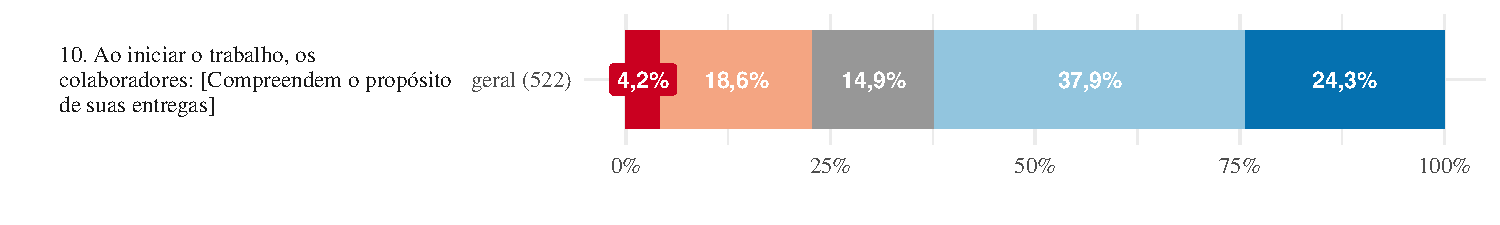
\includegraphics{relatorio_inmetrics_files/figure-latex/aa-1.pdf} 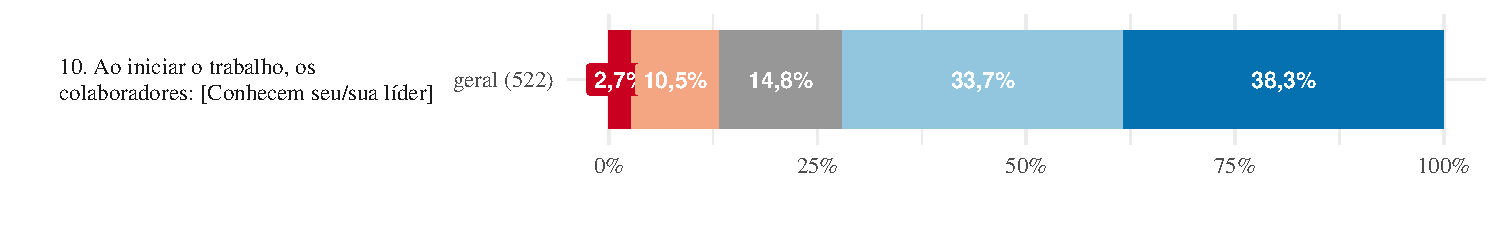
\includegraphics{relatorio_inmetrics_files/figure-latex/aa-2.pdf} 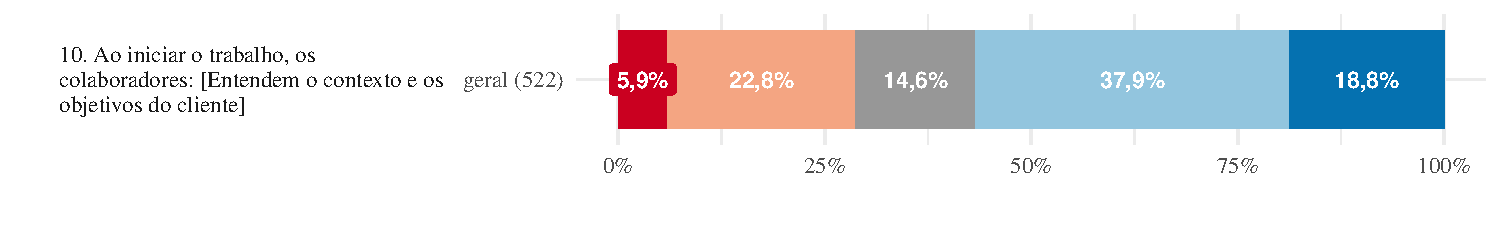
\includegraphics{relatorio_inmetrics_files/figure-latex/aa-3.pdf} 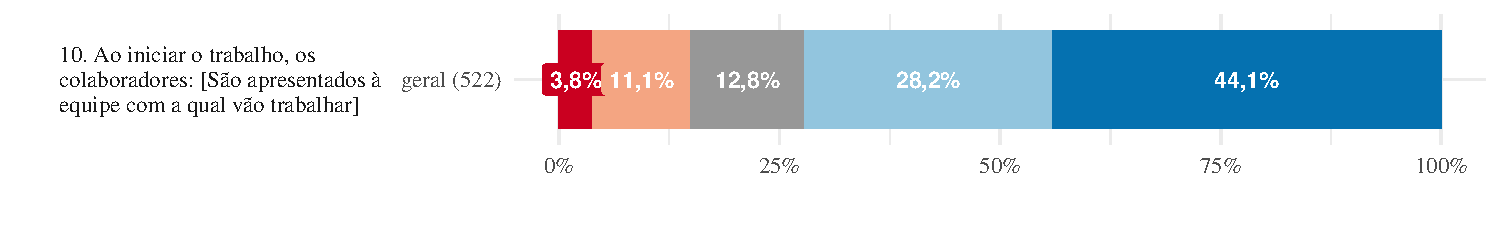
\includegraphics{relatorio_inmetrics_files/figure-latex/aa-4.pdf} 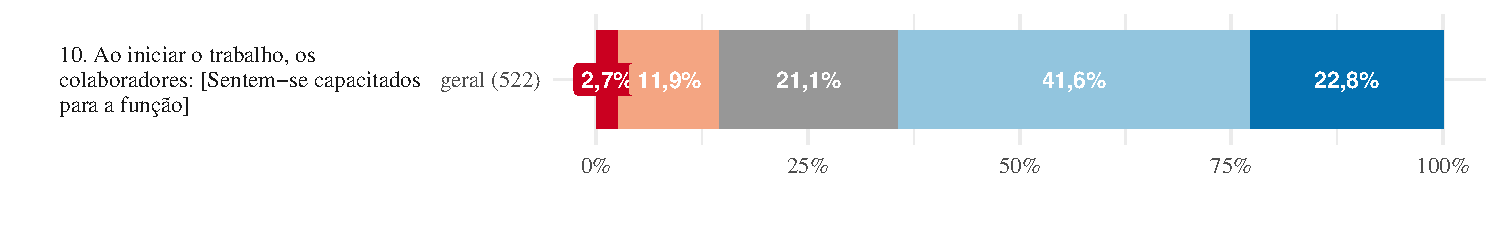
\includegraphics{relatorio_inmetrics_files/figure-latex/aa-5.pdf} 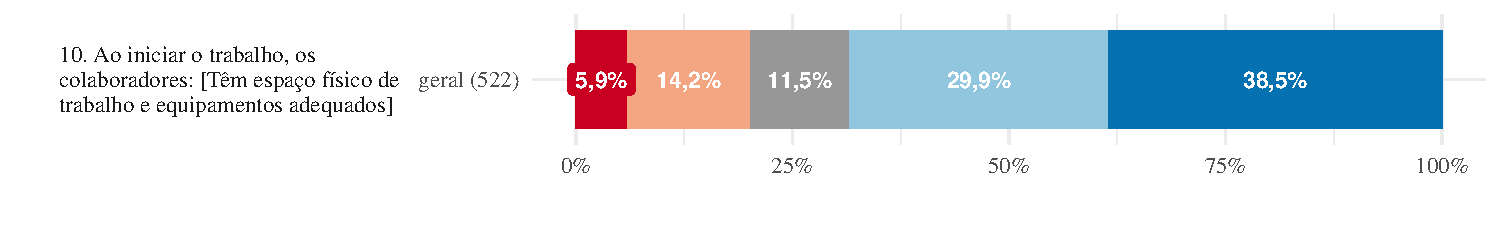
\includegraphics{relatorio_inmetrics_files/figure-latex/aa-6.pdf} 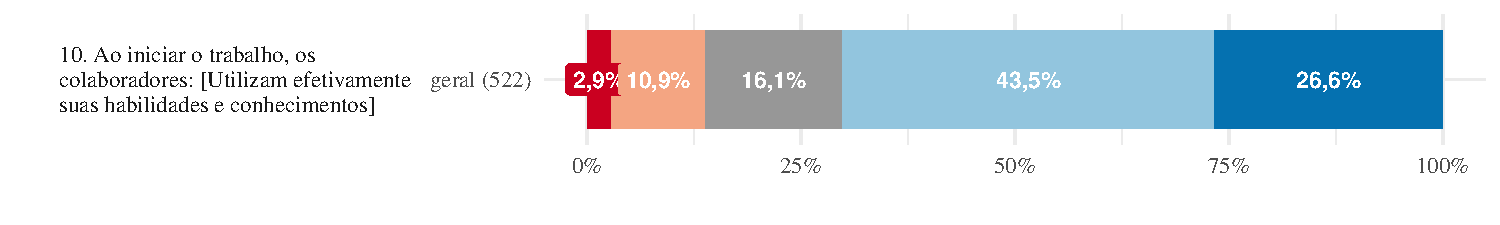
\includegraphics{relatorio_inmetrics_files/figure-latex/aa-7.pdf} 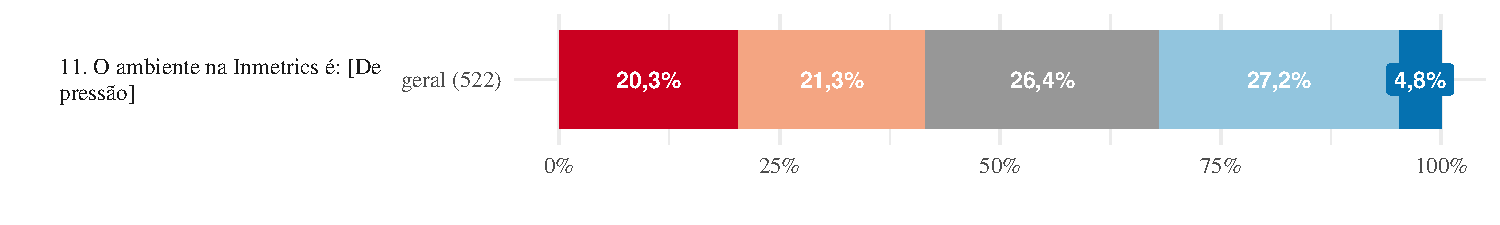
\includegraphics{relatorio_inmetrics_files/figure-latex/aa-8.pdf} 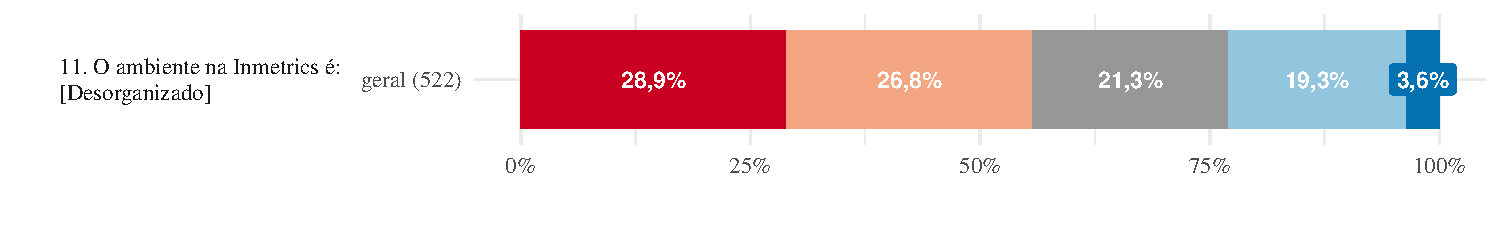
\includegraphics{relatorio_inmetrics_files/figure-latex/aa-9.pdf} 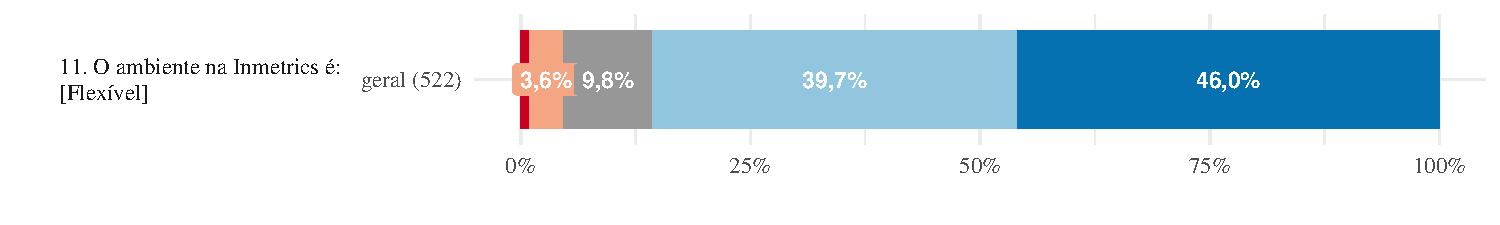
\includegraphics{relatorio_inmetrics_files/figure-latex/aa-10.pdf} 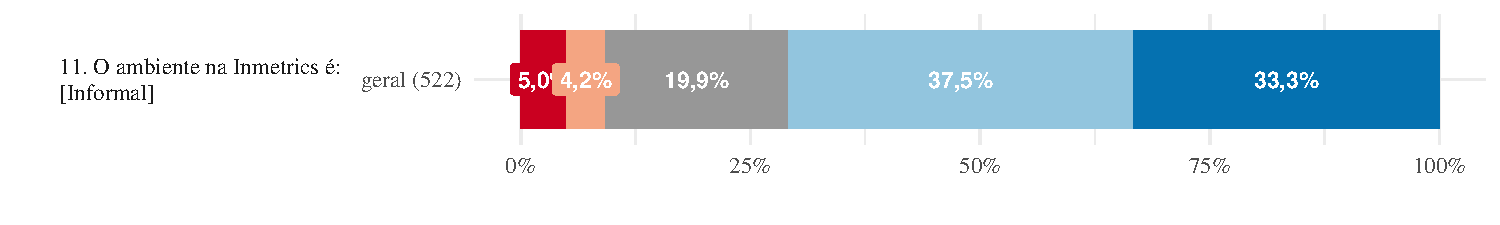
\includegraphics{relatorio_inmetrics_files/figure-latex/aa-11.pdf} 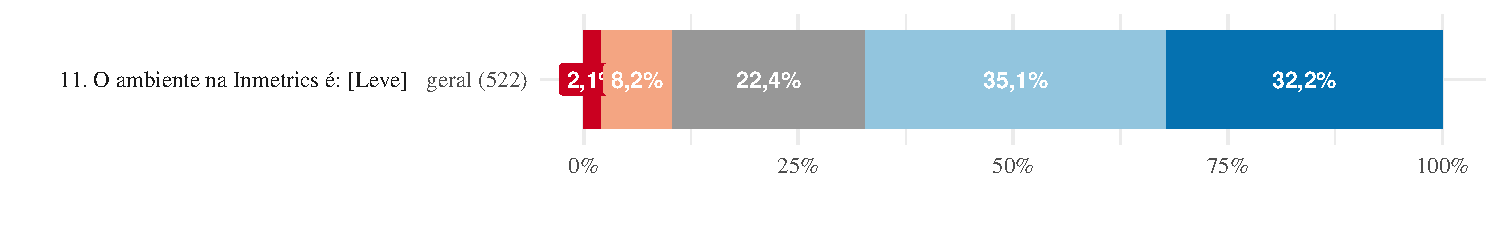
\includegraphics{relatorio_inmetrics_files/figure-latex/aa-12.pdf} 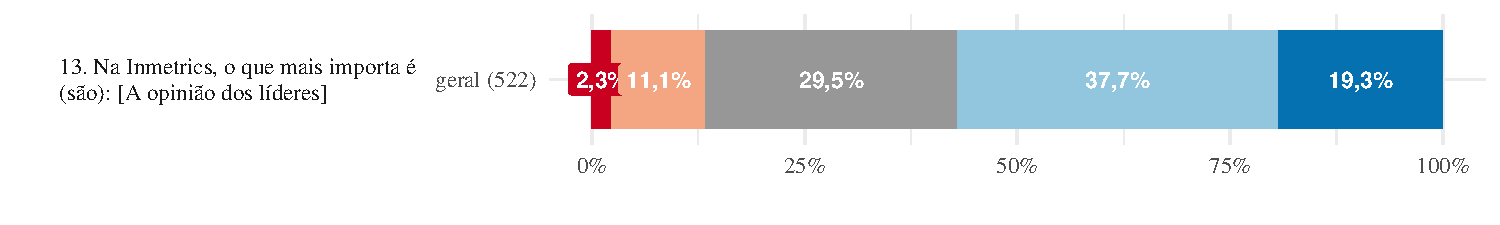
\includegraphics{relatorio_inmetrics_files/figure-latex/aa-13.pdf} 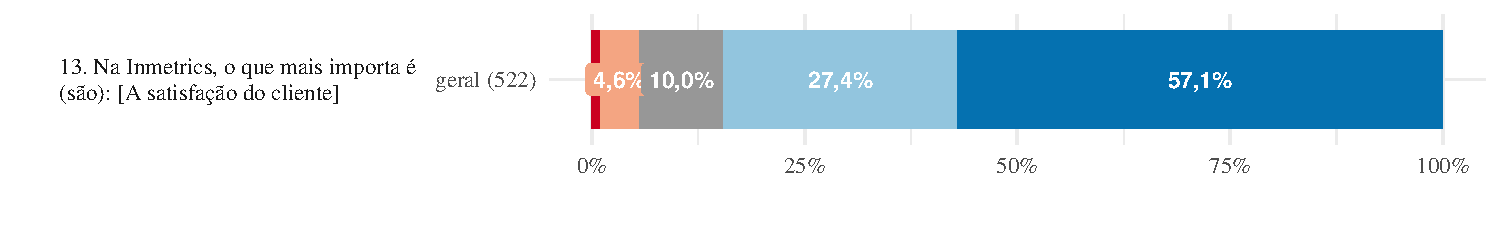
\includegraphics{relatorio_inmetrics_files/figure-latex/aa-14.pdf} 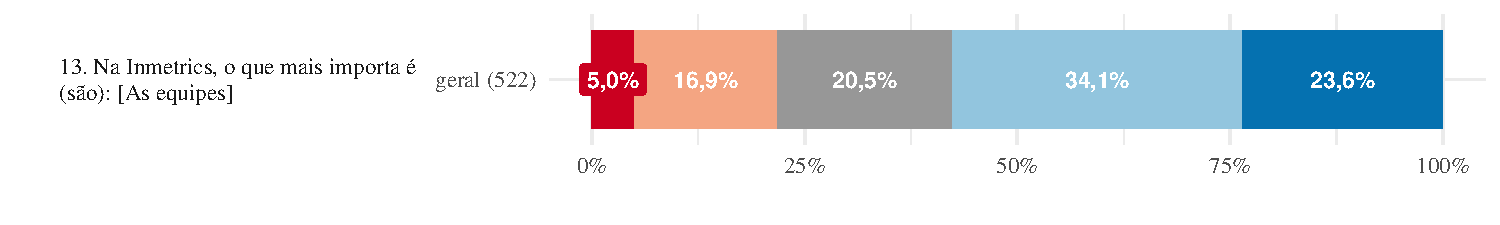
\includegraphics{relatorio_inmetrics_files/figure-latex/aa-15.pdf} 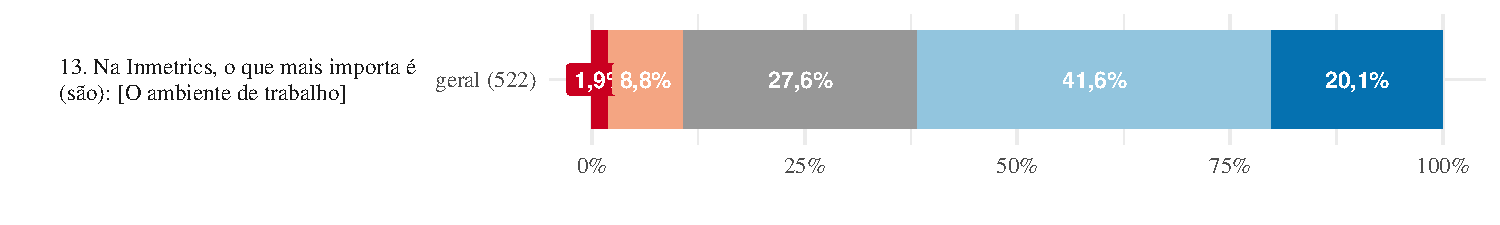
\includegraphics{relatorio_inmetrics_files/figure-latex/aa-16.pdf} 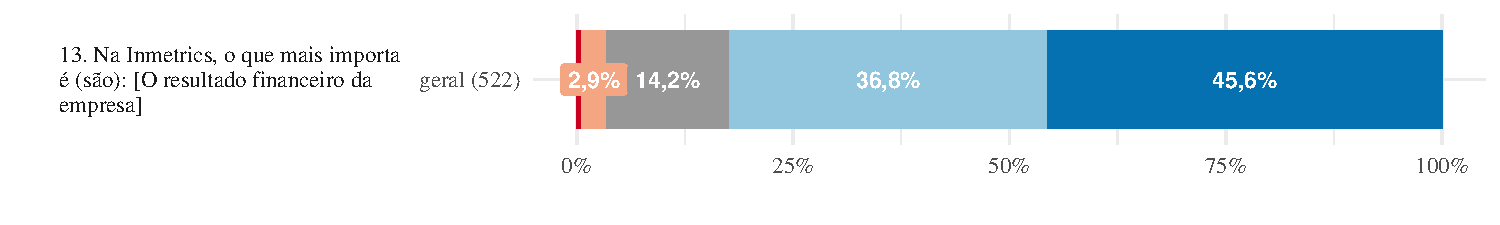
\includegraphics{relatorio_inmetrics_files/figure-latex/aa-17.pdf} 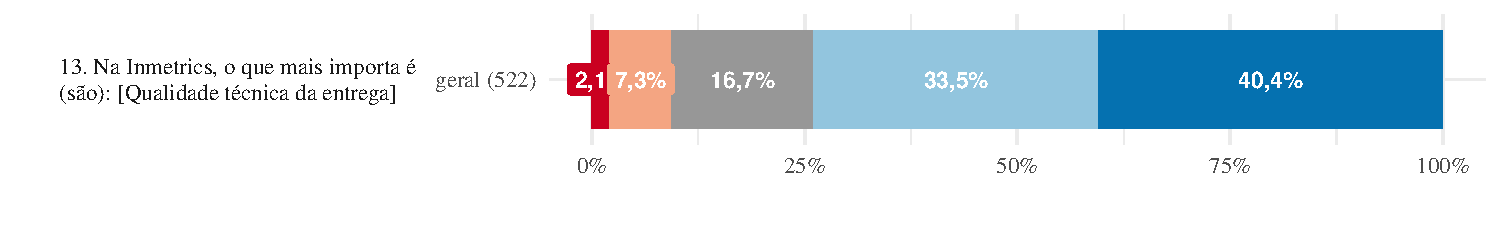
\includegraphics{relatorio_inmetrics_files/figure-latex/aa-18.pdf} 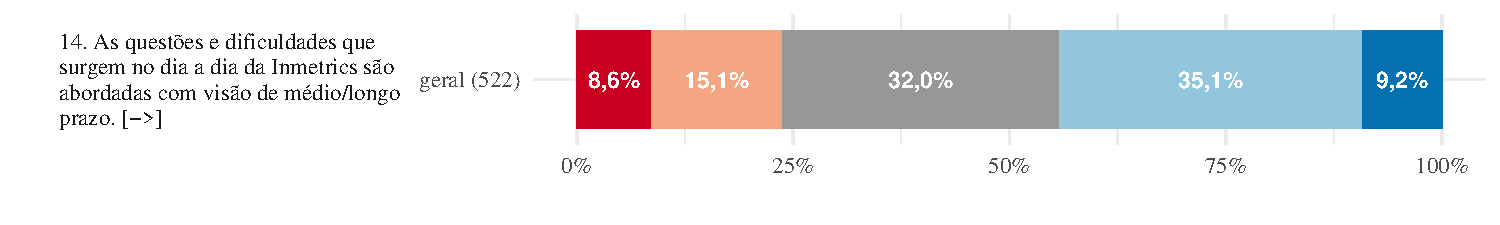
\includegraphics{relatorio_inmetrics_files/figure-latex/aa-19.pdf} 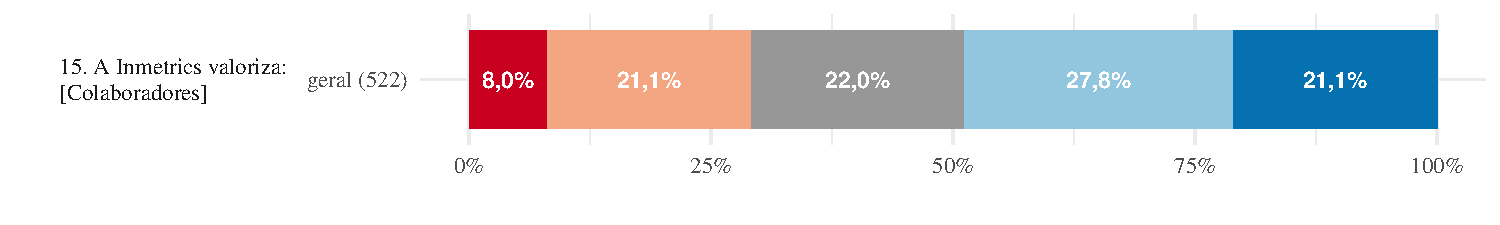
\includegraphics{relatorio_inmetrics_files/figure-latex/aa-20.pdf} 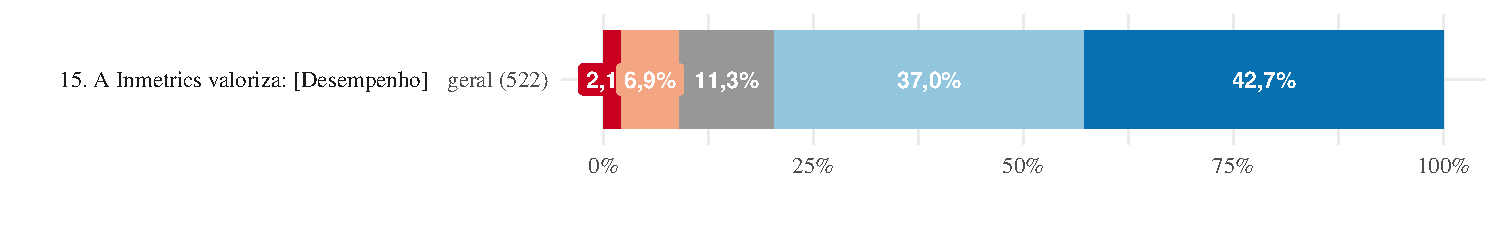
\includegraphics{relatorio_inmetrics_files/figure-latex/aa-21.pdf} 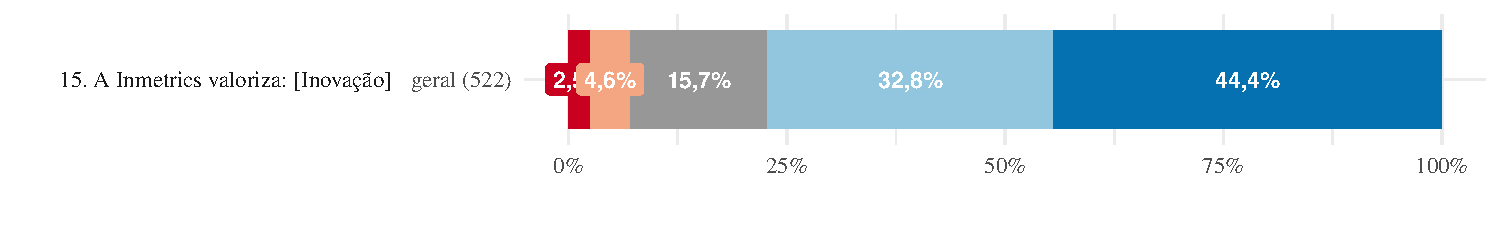
\includegraphics{relatorio_inmetrics_files/figure-latex/aa-22.pdf} 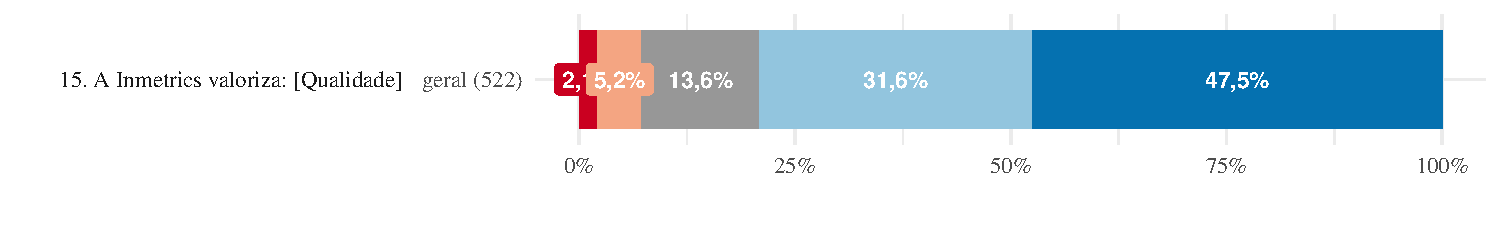
\includegraphics{relatorio_inmetrics_files/figure-latex/aa-23.pdf} 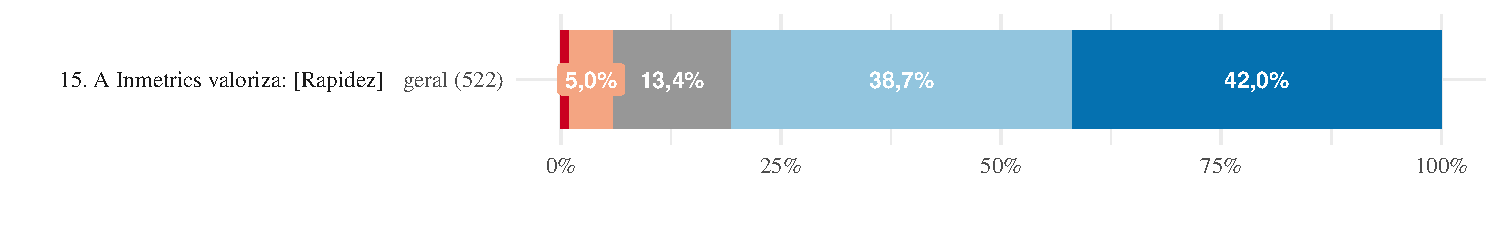
\includegraphics{relatorio_inmetrics_files/figure-latex/aa-24.pdf} 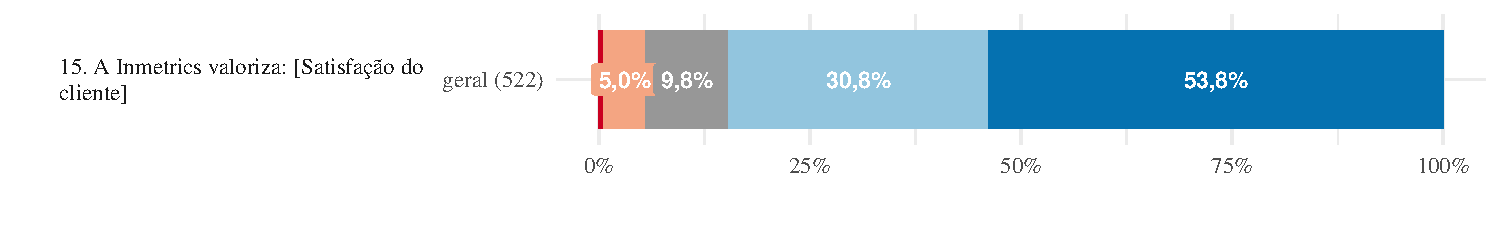
\includegraphics{relatorio_inmetrics_files/figure-latex/aa-25.pdf} 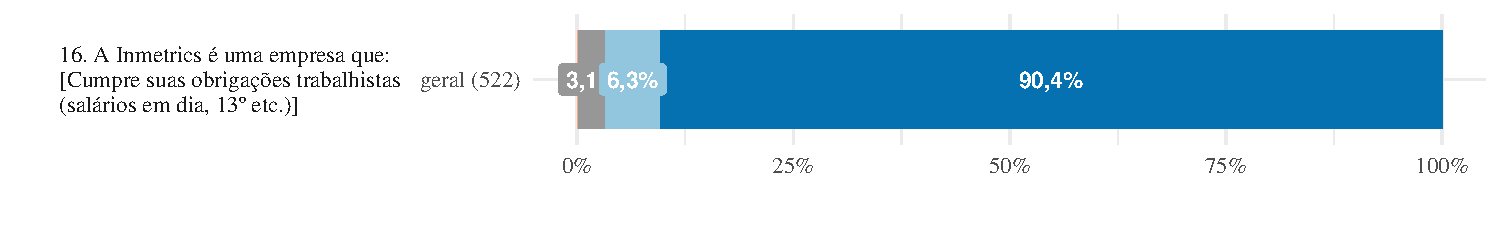
\includegraphics{relatorio_inmetrics_files/figure-latex/aa-26.pdf} 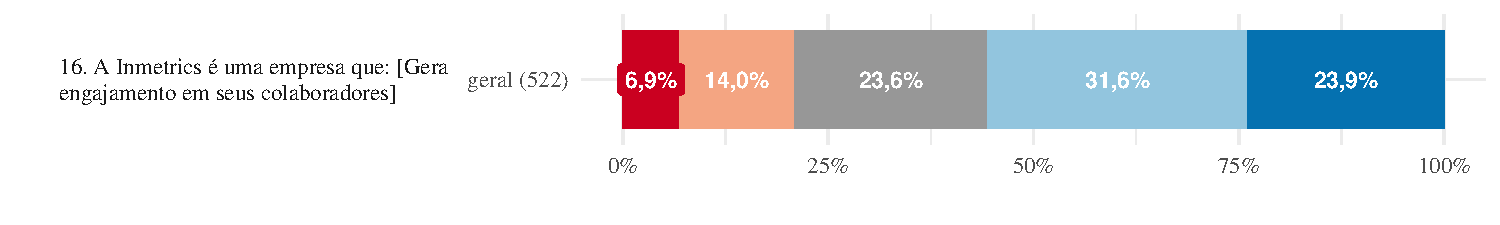
\includegraphics{relatorio_inmetrics_files/figure-latex/aa-27.pdf} 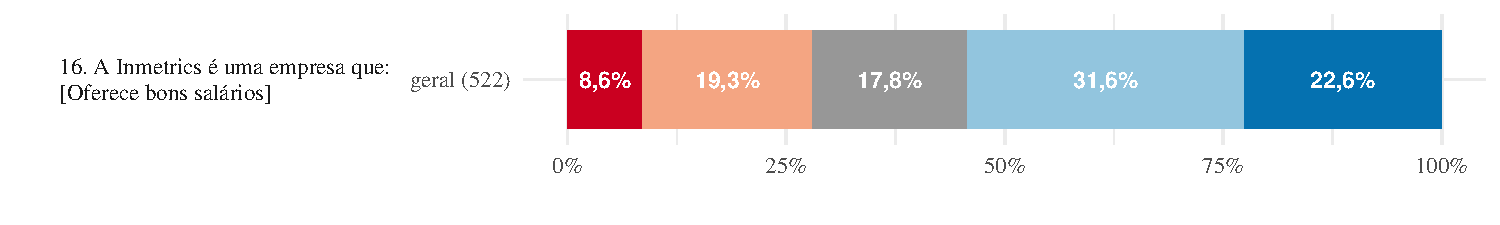
\includegraphics{relatorio_inmetrics_files/figure-latex/aa-28.pdf} 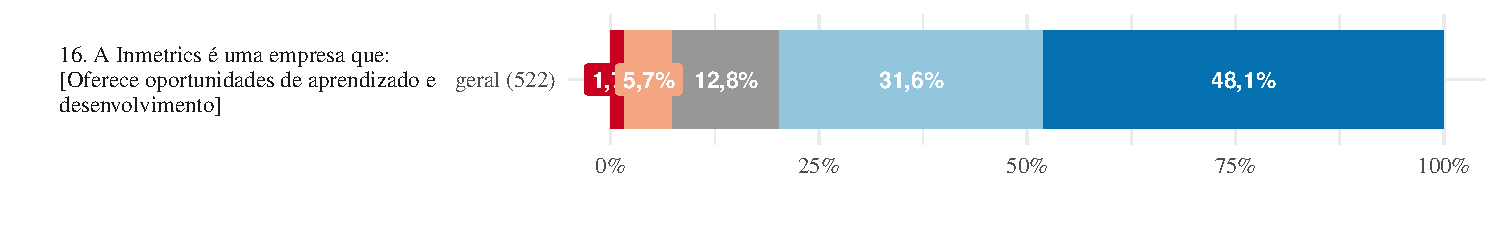
\includegraphics{relatorio_inmetrics_files/figure-latex/aa-29.pdf} 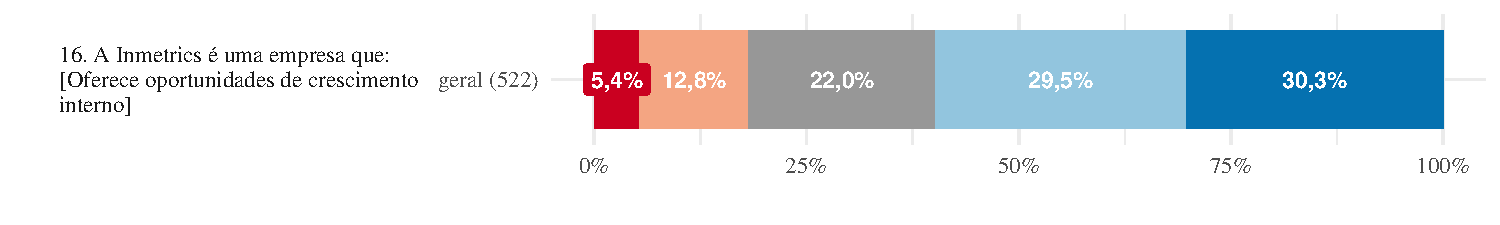
\includegraphics{relatorio_inmetrics_files/figure-latex/aa-30.pdf} 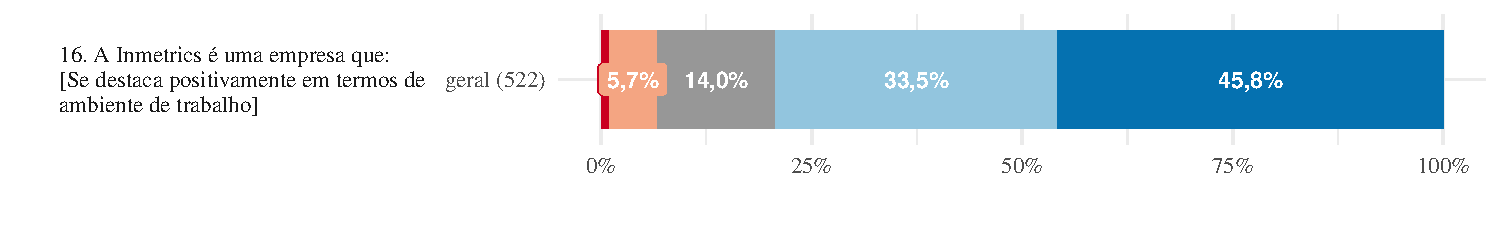
\includegraphics{relatorio_inmetrics_files/figure-latex/aa-31.pdf} 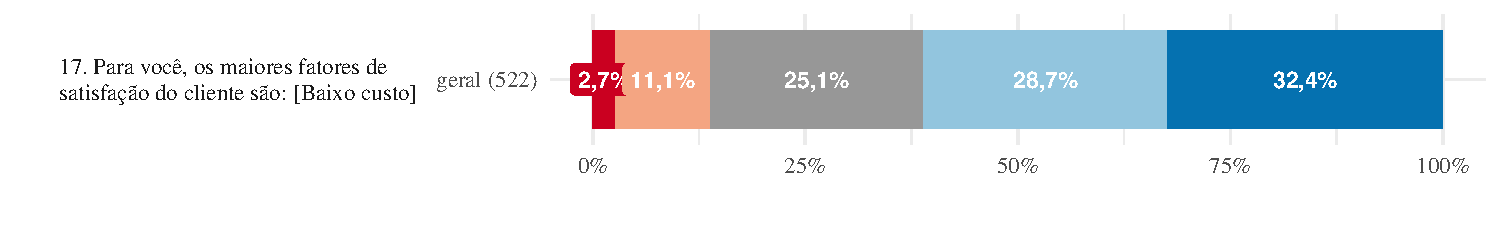
\includegraphics{relatorio_inmetrics_files/figure-latex/aa-32.pdf} 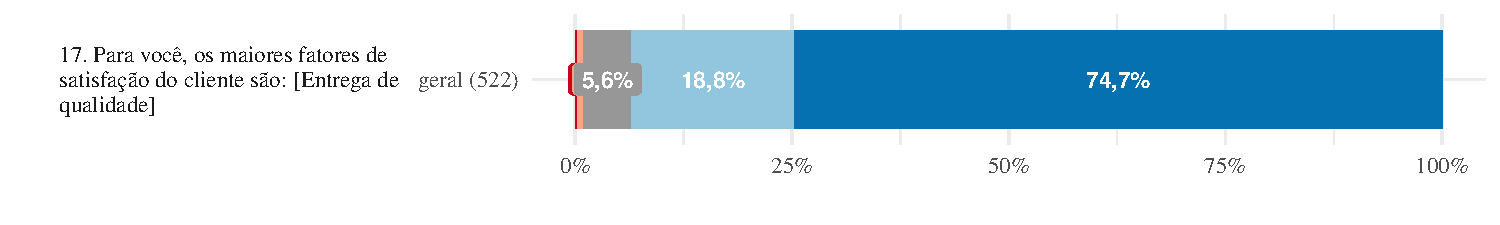
\includegraphics{relatorio_inmetrics_files/figure-latex/aa-33.pdf} 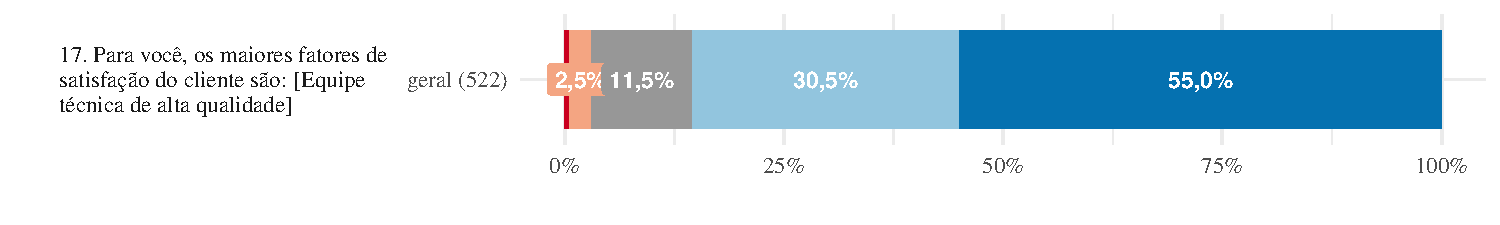
\includegraphics{relatorio_inmetrics_files/figure-latex/aa-34.pdf} 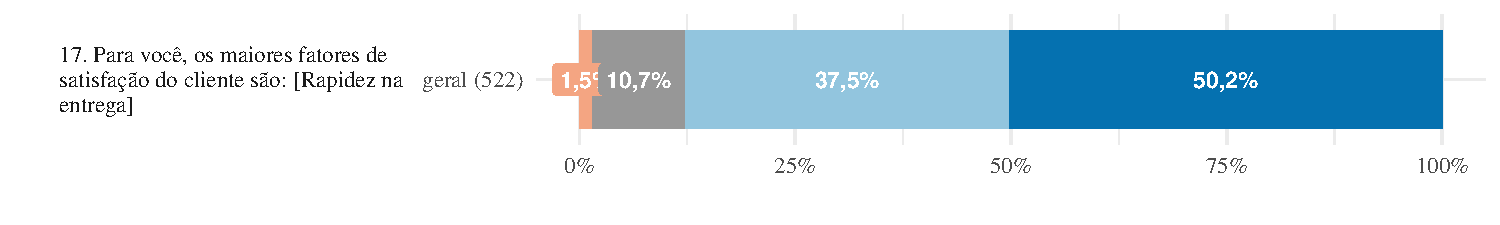
\includegraphics{relatorio_inmetrics_files/figure-latex/aa-35.pdf} 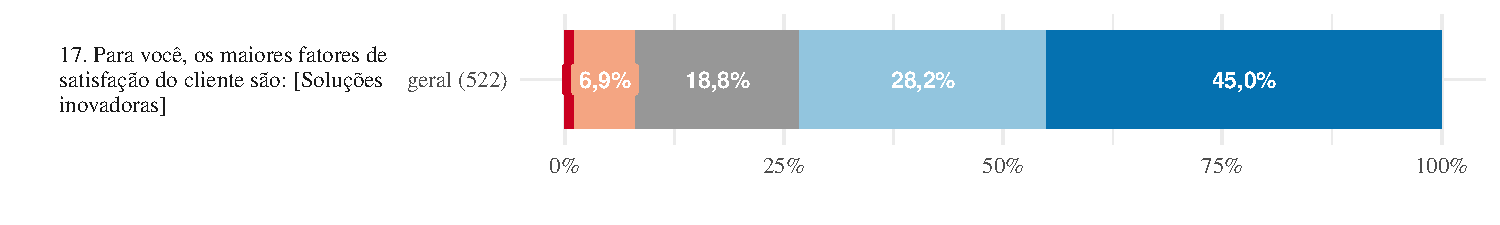
\includegraphics{relatorio_inmetrics_files/figure-latex/aa-36.pdf} 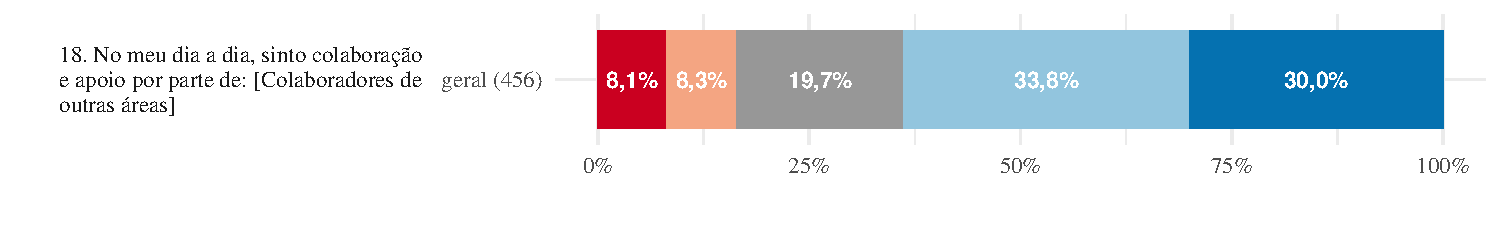
\includegraphics{relatorio_inmetrics_files/figure-latex/aa-37.pdf} 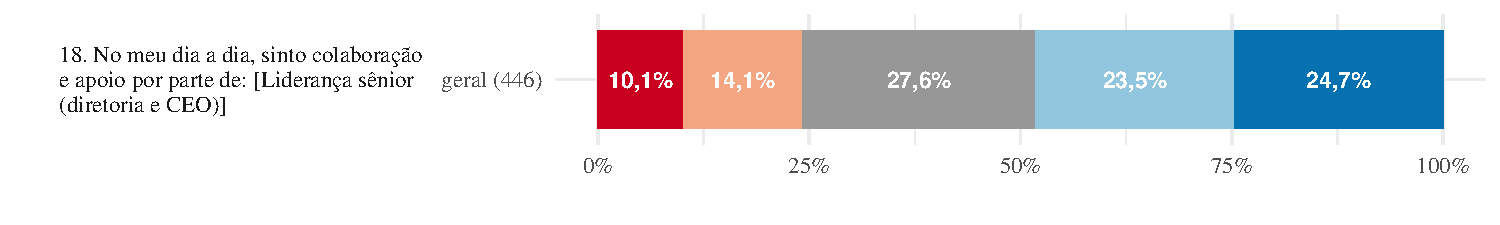
\includegraphics{relatorio_inmetrics_files/figure-latex/aa-38.pdf} 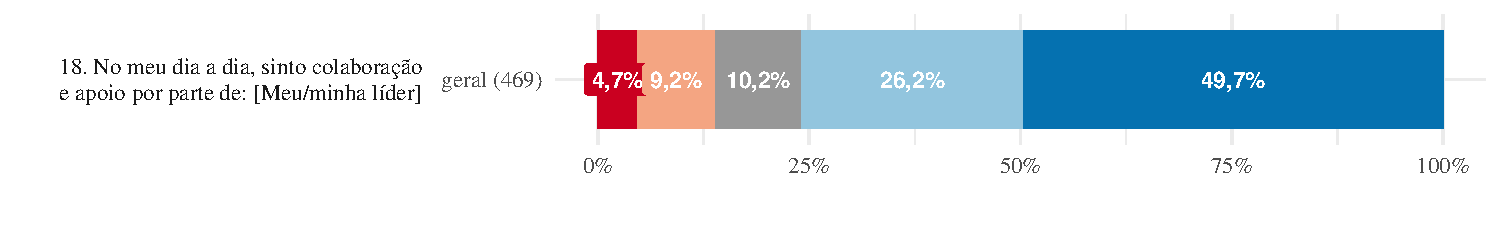
\includegraphics{relatorio_inmetrics_files/figure-latex/aa-39.pdf} 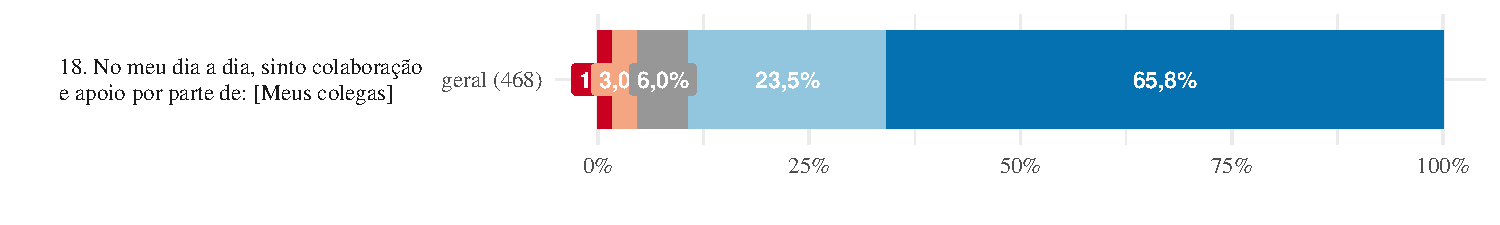
\includegraphics{relatorio_inmetrics_files/figure-latex/aa-40.pdf} 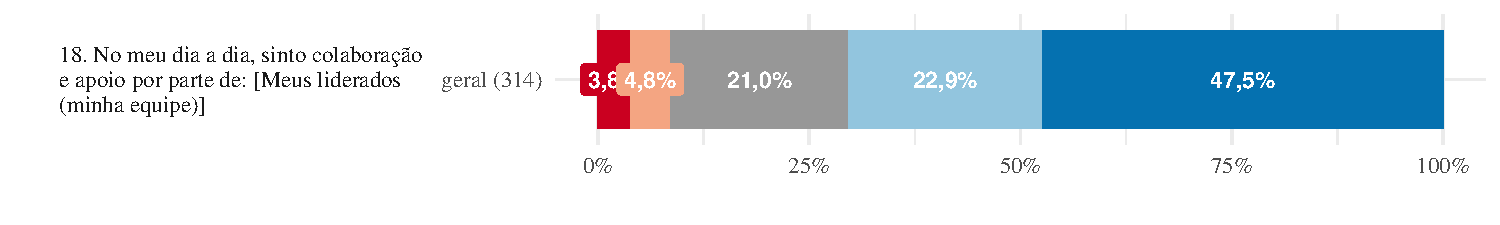
\includegraphics{relatorio_inmetrics_files/figure-latex/aa-41.pdf} 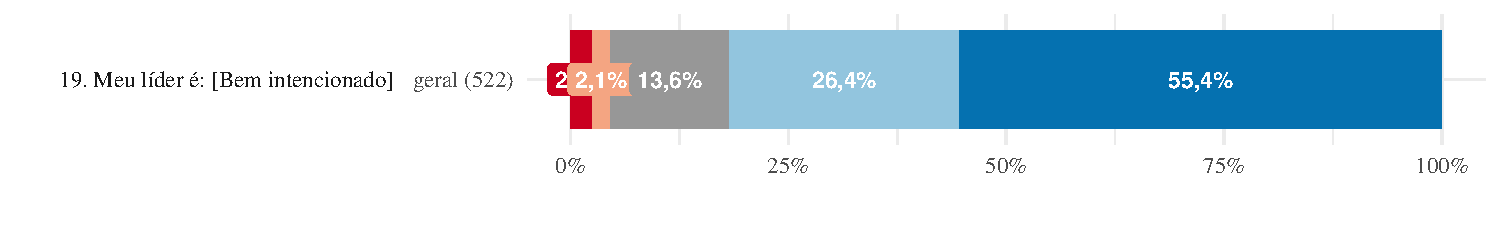
\includegraphics{relatorio_inmetrics_files/figure-latex/aa-42.pdf} 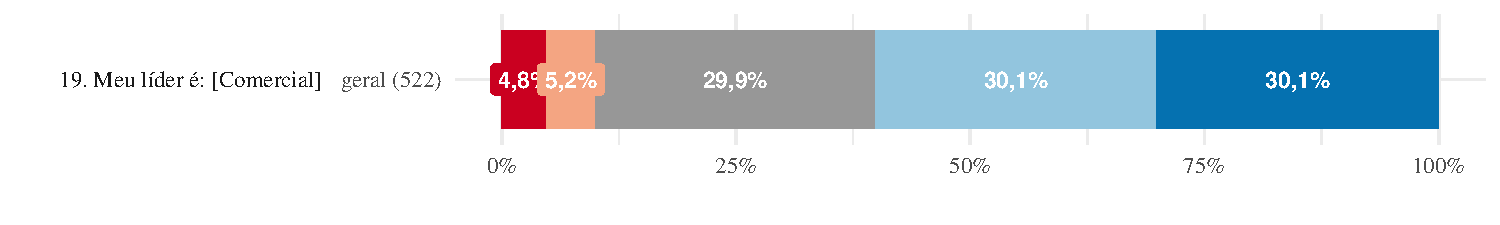
\includegraphics{relatorio_inmetrics_files/figure-latex/aa-43.pdf} 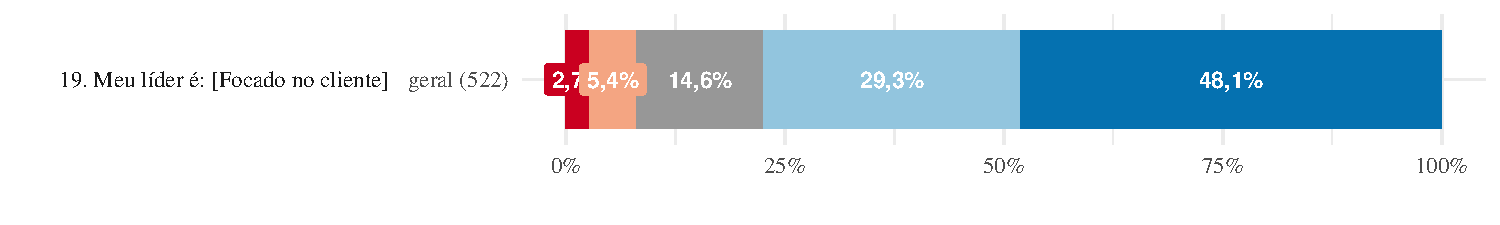
\includegraphics{relatorio_inmetrics_files/figure-latex/aa-44.pdf} 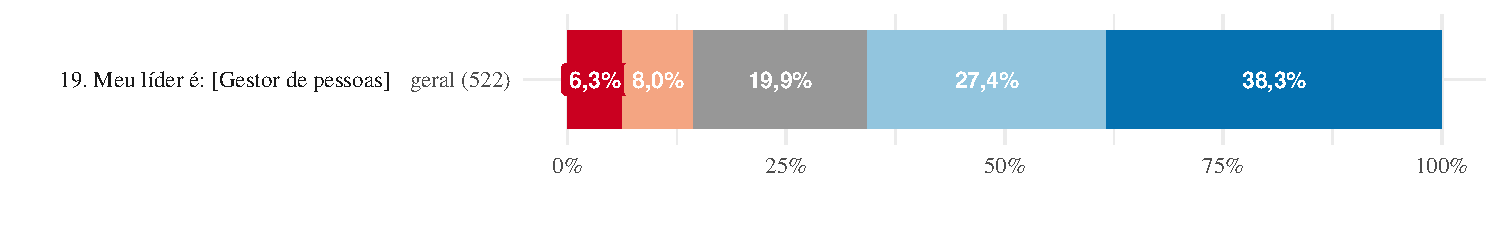
\includegraphics{relatorio_inmetrics_files/figure-latex/aa-45.pdf} 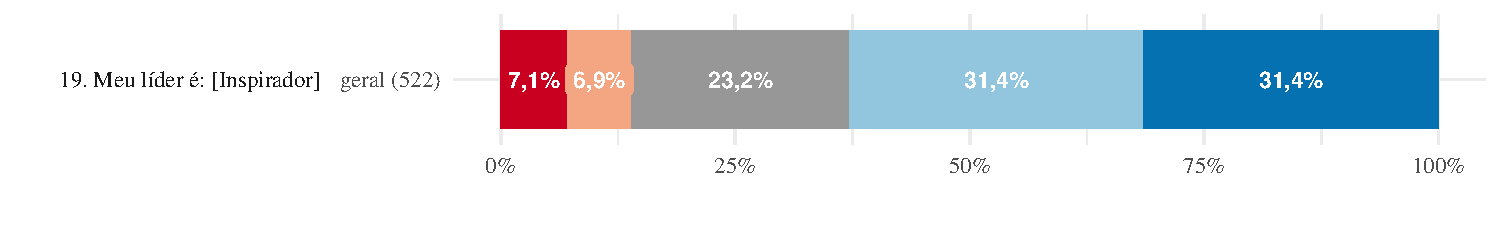
\includegraphics{relatorio_inmetrics_files/figure-latex/aa-46.pdf} 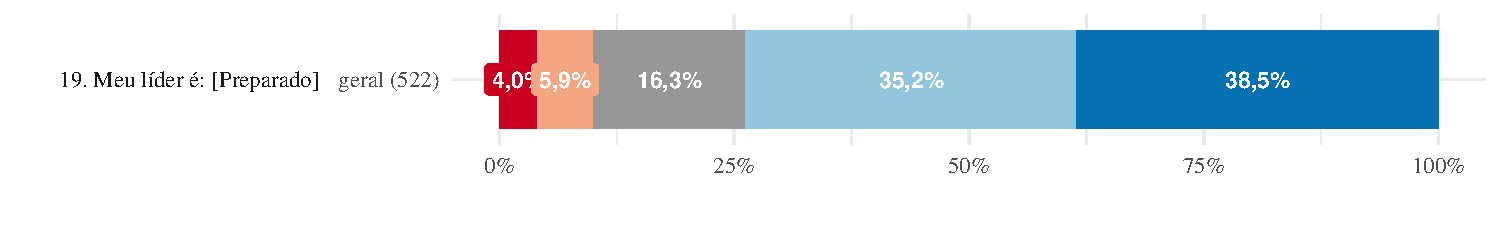
\includegraphics{relatorio_inmetrics_files/figure-latex/aa-47.pdf} 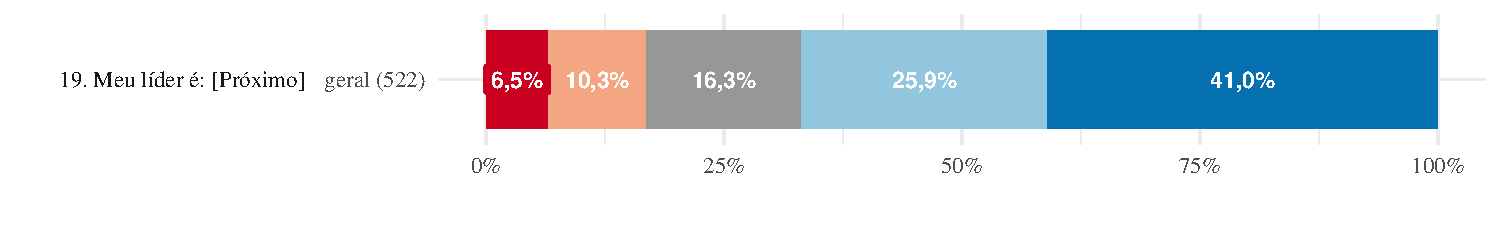
\includegraphics{relatorio_inmetrics_files/figure-latex/aa-48.pdf} 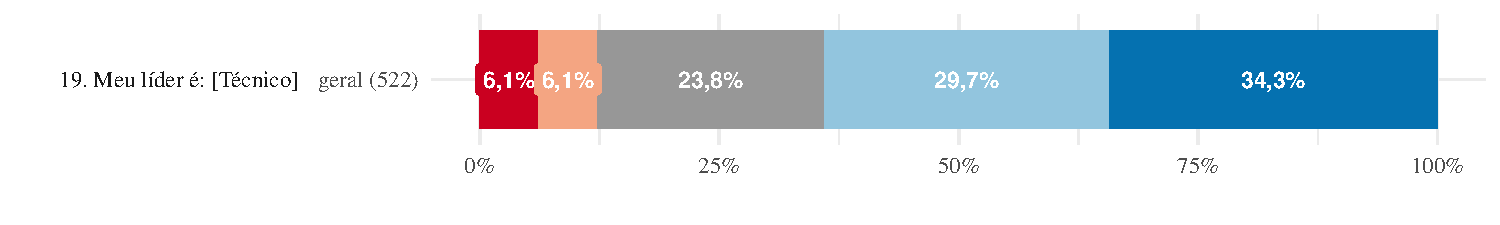
\includegraphics{relatorio_inmetrics_files/figure-latex/aa-49.pdf} 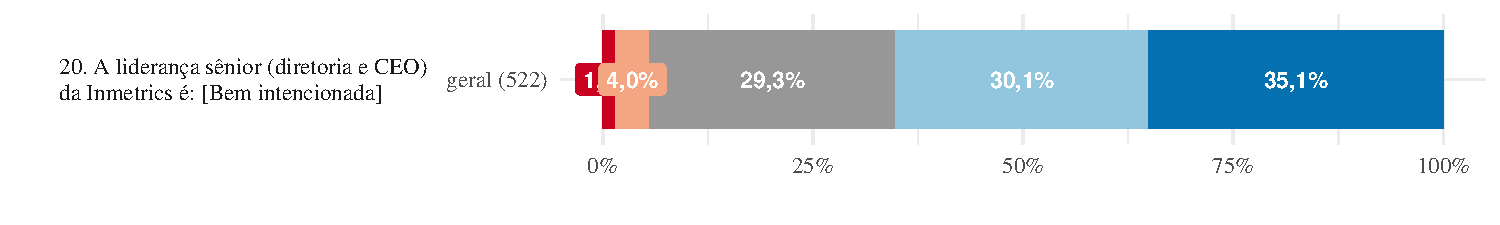
\includegraphics{relatorio_inmetrics_files/figure-latex/aa-50.pdf} \includegraphics{relatorio_inmetrics_files/figure-latex/aa-51.pdf} \includegraphics{relatorio_inmetrics_files/figure-latex/aa-52.pdf} \includegraphics{relatorio_inmetrics_files/figure-latex/aa-53.pdf} \includegraphics{relatorio_inmetrics_files/figure-latex/aa-54.pdf} \includegraphics{relatorio_inmetrics_files/figure-latex/aa-55.pdf} \includegraphics{relatorio_inmetrics_files/figure-latex/aa-56.pdf} \includegraphics{relatorio_inmetrics_files/figure-latex/aa-57.pdf} \includegraphics{relatorio_inmetrics_files/figure-latex/aa-58.pdf} \includegraphics{relatorio_inmetrics_files/figure-latex/aa-59.pdf} \includegraphics{relatorio_inmetrics_files/figure-latex/aa-60.pdf} \includegraphics{relatorio_inmetrics_files/figure-latex/aa-61.pdf} \includegraphics{relatorio_inmetrics_files/figure-latex/aa-62.pdf} \includegraphics{relatorio_inmetrics_files/figure-latex/aa-63.pdf} \includegraphics{relatorio_inmetrics_files/figure-latex/aa-64.pdf} \includegraphics{relatorio_inmetrics_files/figure-latex/aa-65.pdf} \includegraphics{relatorio_inmetrics_files/figure-latex/aa-66.pdf} \includegraphics{relatorio_inmetrics_files/figure-latex/aa-67.pdf} \includegraphics{relatorio_inmetrics_files/figure-latex/aa-68.pdf}

\hypertarget{questoes-por-posicao-eu-sou}{%
\section{Questões por Posição (Eu sou\ldots{})}\label{questoes-por-posicao-eu-sou}}

\includegraphics{relatorio_inmetrics_files/figure-latex/cc-1.pdf} \includegraphics{relatorio_inmetrics_files/figure-latex/cc-2.pdf} \includegraphics{relatorio_inmetrics_files/figure-latex/cc-3.pdf} \includegraphics{relatorio_inmetrics_files/figure-latex/cc-4.pdf} \includegraphics{relatorio_inmetrics_files/figure-latex/cc-5.pdf} \includegraphics{relatorio_inmetrics_files/figure-latex/cc-6.pdf} \includegraphics{relatorio_inmetrics_files/figure-latex/cc-7.pdf} \includegraphics{relatorio_inmetrics_files/figure-latex/cc-8.pdf} \includegraphics{relatorio_inmetrics_files/figure-latex/cc-9.pdf} \includegraphics{relatorio_inmetrics_files/figure-latex/cc-10.pdf} \includegraphics{relatorio_inmetrics_files/figure-latex/cc-11.pdf} \includegraphics{relatorio_inmetrics_files/figure-latex/cc-12.pdf} \includegraphics{relatorio_inmetrics_files/figure-latex/cc-13.pdf} \includegraphics{relatorio_inmetrics_files/figure-latex/cc-14.pdf} \includegraphics{relatorio_inmetrics_files/figure-latex/cc-15.pdf} \includegraphics{relatorio_inmetrics_files/figure-latex/cc-16.pdf} \includegraphics{relatorio_inmetrics_files/figure-latex/cc-17.pdf} \includegraphics{relatorio_inmetrics_files/figure-latex/cc-18.pdf} \includegraphics{relatorio_inmetrics_files/figure-latex/cc-19.pdf} \includegraphics{relatorio_inmetrics_files/figure-latex/cc-20.pdf} \includegraphics{relatorio_inmetrics_files/figure-latex/cc-21.pdf} \includegraphics{relatorio_inmetrics_files/figure-latex/cc-22.pdf} \includegraphics{relatorio_inmetrics_files/figure-latex/cc-23.pdf} \includegraphics{relatorio_inmetrics_files/figure-latex/cc-24.pdf} \includegraphics{relatorio_inmetrics_files/figure-latex/cc-25.pdf} \includegraphics{relatorio_inmetrics_files/figure-latex/cc-26.pdf} \includegraphics{relatorio_inmetrics_files/figure-latex/cc-27.pdf} \includegraphics{relatorio_inmetrics_files/figure-latex/cc-28.pdf} \includegraphics{relatorio_inmetrics_files/figure-latex/cc-29.pdf} \includegraphics{relatorio_inmetrics_files/figure-latex/cc-30.pdf} \includegraphics{relatorio_inmetrics_files/figure-latex/cc-31.pdf} \includegraphics{relatorio_inmetrics_files/figure-latex/cc-32.pdf} \includegraphics{relatorio_inmetrics_files/figure-latex/cc-33.pdf} \includegraphics{relatorio_inmetrics_files/figure-latex/cc-34.pdf} \includegraphics{relatorio_inmetrics_files/figure-latex/cc-35.pdf} \includegraphics{relatorio_inmetrics_files/figure-latex/cc-36.pdf} \includegraphics{relatorio_inmetrics_files/figure-latex/cc-37.pdf} \includegraphics{relatorio_inmetrics_files/figure-latex/cc-38.pdf} \includegraphics{relatorio_inmetrics_files/figure-latex/cc-39.pdf} \includegraphics{relatorio_inmetrics_files/figure-latex/cc-40.pdf} \includegraphics{relatorio_inmetrics_files/figure-latex/cc-41.pdf} \includegraphics{relatorio_inmetrics_files/figure-latex/cc-42.pdf} \includegraphics{relatorio_inmetrics_files/figure-latex/cc-43.pdf} \includegraphics{relatorio_inmetrics_files/figure-latex/cc-44.pdf} \includegraphics{relatorio_inmetrics_files/figure-latex/cc-45.pdf} \includegraphics{relatorio_inmetrics_files/figure-latex/cc-46.pdf} \includegraphics{relatorio_inmetrics_files/figure-latex/cc-47.pdf} \includegraphics{relatorio_inmetrics_files/figure-latex/cc-48.pdf} \includegraphics{relatorio_inmetrics_files/figure-latex/cc-49.pdf} \includegraphics{relatorio_inmetrics_files/figure-latex/cc-50.pdf} \includegraphics{relatorio_inmetrics_files/figure-latex/cc-51.pdf} \includegraphics{relatorio_inmetrics_files/figure-latex/cc-52.pdf} \includegraphics{relatorio_inmetrics_files/figure-latex/cc-53.pdf} \includegraphics{relatorio_inmetrics_files/figure-latex/cc-54.pdf} \includegraphics{relatorio_inmetrics_files/figure-latex/cc-55.pdf} \includegraphics{relatorio_inmetrics_files/figure-latex/cc-56.pdf} \includegraphics{relatorio_inmetrics_files/figure-latex/cc-57.pdf} \includegraphics{relatorio_inmetrics_files/figure-latex/cc-58.pdf} \includegraphics{relatorio_inmetrics_files/figure-latex/cc-59.pdf} \includegraphics{relatorio_inmetrics_files/figure-latex/cc-60.pdf} \includegraphics{relatorio_inmetrics_files/figure-latex/cc-61.pdf} \includegraphics{relatorio_inmetrics_files/figure-latex/cc-62.pdf} \includegraphics{relatorio_inmetrics_files/figure-latex/cc-63.pdf} \includegraphics{relatorio_inmetrics_files/figure-latex/cc-64.pdf} \includegraphics{relatorio_inmetrics_files/figure-latex/cc-65.pdf} \includegraphics{relatorio_inmetrics_files/figure-latex/cc-66.pdf} \includegraphics{relatorio_inmetrics_files/figure-latex/cc-67.pdf} \includegraphics{relatorio_inmetrics_files/figure-latex/cc-68.pdf}

\hypertarget{questoes-por-area}{%
\section{Questões por Área}\label{questoes-por-area}}

\includegraphics{relatorio_inmetrics_files/figure-latex/ee-1.pdf} \includegraphics{relatorio_inmetrics_files/figure-latex/ee-2.pdf} \includegraphics{relatorio_inmetrics_files/figure-latex/ee-3.pdf} \includegraphics{relatorio_inmetrics_files/figure-latex/ee-4.pdf} \includegraphics{relatorio_inmetrics_files/figure-latex/ee-5.pdf} \includegraphics{relatorio_inmetrics_files/figure-latex/ee-6.pdf} \includegraphics{relatorio_inmetrics_files/figure-latex/ee-7.pdf} \includegraphics{relatorio_inmetrics_files/figure-latex/ee-8.pdf} \includegraphics{relatorio_inmetrics_files/figure-latex/ee-9.pdf} \includegraphics{relatorio_inmetrics_files/figure-latex/ee-10.pdf} \includegraphics{relatorio_inmetrics_files/figure-latex/ee-11.pdf} \includegraphics{relatorio_inmetrics_files/figure-latex/ee-12.pdf} \includegraphics{relatorio_inmetrics_files/figure-latex/ee-13.pdf} \includegraphics{relatorio_inmetrics_files/figure-latex/ee-14.pdf} \includegraphics{relatorio_inmetrics_files/figure-latex/ee-15.pdf} \includegraphics{relatorio_inmetrics_files/figure-latex/ee-16.pdf} \includegraphics{relatorio_inmetrics_files/figure-latex/ee-17.pdf} \includegraphics{relatorio_inmetrics_files/figure-latex/ee-18.pdf} \includegraphics{relatorio_inmetrics_files/figure-latex/ee-19.pdf} \includegraphics{relatorio_inmetrics_files/figure-latex/ee-20.pdf} \includegraphics{relatorio_inmetrics_files/figure-latex/ee-21.pdf} \includegraphics{relatorio_inmetrics_files/figure-latex/ee-22.pdf} \includegraphics{relatorio_inmetrics_files/figure-latex/ee-23.pdf} \includegraphics{relatorio_inmetrics_files/figure-latex/ee-24.pdf} \includegraphics{relatorio_inmetrics_files/figure-latex/ee-25.pdf} \includegraphics{relatorio_inmetrics_files/figure-latex/ee-26.pdf} \includegraphics{relatorio_inmetrics_files/figure-latex/ee-27.pdf} \includegraphics{relatorio_inmetrics_files/figure-latex/ee-28.pdf} \includegraphics{relatorio_inmetrics_files/figure-latex/ee-29.pdf} \includegraphics{relatorio_inmetrics_files/figure-latex/ee-30.pdf} \includegraphics{relatorio_inmetrics_files/figure-latex/ee-31.pdf} \includegraphics{relatorio_inmetrics_files/figure-latex/ee-32.pdf} \includegraphics{relatorio_inmetrics_files/figure-latex/ee-33.pdf} \includegraphics{relatorio_inmetrics_files/figure-latex/ee-34.pdf} \includegraphics{relatorio_inmetrics_files/figure-latex/ee-35.pdf} \includegraphics{relatorio_inmetrics_files/figure-latex/ee-36.pdf} \includegraphics{relatorio_inmetrics_files/figure-latex/ee-37.pdf} \includegraphics{relatorio_inmetrics_files/figure-latex/ee-38.pdf} \includegraphics{relatorio_inmetrics_files/figure-latex/ee-39.pdf} \includegraphics{relatorio_inmetrics_files/figure-latex/ee-40.pdf} \includegraphics{relatorio_inmetrics_files/figure-latex/ee-41.pdf} \includegraphics{relatorio_inmetrics_files/figure-latex/ee-42.pdf} \includegraphics{relatorio_inmetrics_files/figure-latex/ee-43.pdf} \includegraphics{relatorio_inmetrics_files/figure-latex/ee-44.pdf} \includegraphics{relatorio_inmetrics_files/figure-latex/ee-45.pdf} \includegraphics{relatorio_inmetrics_files/figure-latex/ee-46.pdf} \includegraphics{relatorio_inmetrics_files/figure-latex/ee-47.pdf} \includegraphics{relatorio_inmetrics_files/figure-latex/ee-48.pdf} \includegraphics{relatorio_inmetrics_files/figure-latex/ee-49.pdf} \includegraphics{relatorio_inmetrics_files/figure-latex/ee-50.pdf} \includegraphics{relatorio_inmetrics_files/figure-latex/ee-51.pdf} \includegraphics{relatorio_inmetrics_files/figure-latex/ee-52.pdf} \includegraphics{relatorio_inmetrics_files/figure-latex/ee-53.pdf} \includegraphics{relatorio_inmetrics_files/figure-latex/ee-54.pdf} \includegraphics{relatorio_inmetrics_files/figure-latex/ee-55.pdf} \includegraphics{relatorio_inmetrics_files/figure-latex/ee-56.pdf} \includegraphics{relatorio_inmetrics_files/figure-latex/ee-57.pdf} \includegraphics{relatorio_inmetrics_files/figure-latex/ee-58.pdf} \includegraphics{relatorio_inmetrics_files/figure-latex/ee-59.pdf} \includegraphics{relatorio_inmetrics_files/figure-latex/ee-60.pdf} \includegraphics{relatorio_inmetrics_files/figure-latex/ee-61.pdf} \includegraphics{relatorio_inmetrics_files/figure-latex/ee-62.pdf} \includegraphics{relatorio_inmetrics_files/figure-latex/ee-63.pdf} \includegraphics{relatorio_inmetrics_files/figure-latex/ee-64.pdf} \includegraphics{relatorio_inmetrics_files/figure-latex/ee-65.pdf} \includegraphics{relatorio_inmetrics_files/figure-latex/ee-66.pdf} \includegraphics{relatorio_inmetrics_files/figure-latex/ee-67.pdf} \includegraphics{relatorio_inmetrics_files/figure-latex/ee-68.pdf}

\hypertarget{questoes-por-genero}{%
\section{Questões por Gênero}\label{questoes-por-genero}}

\includegraphics{relatorio_inmetrics_files/figure-latex/gg-1.pdf} \includegraphics{relatorio_inmetrics_files/figure-latex/gg-2.pdf} \includegraphics{relatorio_inmetrics_files/figure-latex/gg-3.pdf} \includegraphics{relatorio_inmetrics_files/figure-latex/gg-4.pdf} \includegraphics{relatorio_inmetrics_files/figure-latex/gg-5.pdf} \includegraphics{relatorio_inmetrics_files/figure-latex/gg-6.pdf} \includegraphics{relatorio_inmetrics_files/figure-latex/gg-7.pdf} \includegraphics{relatorio_inmetrics_files/figure-latex/gg-8.pdf} \includegraphics{relatorio_inmetrics_files/figure-latex/gg-9.pdf} \includegraphics{relatorio_inmetrics_files/figure-latex/gg-10.pdf} \includegraphics{relatorio_inmetrics_files/figure-latex/gg-11.pdf} \includegraphics{relatorio_inmetrics_files/figure-latex/gg-12.pdf} \includegraphics{relatorio_inmetrics_files/figure-latex/gg-13.pdf} \includegraphics{relatorio_inmetrics_files/figure-latex/gg-14.pdf} \includegraphics{relatorio_inmetrics_files/figure-latex/gg-15.pdf} \includegraphics{relatorio_inmetrics_files/figure-latex/gg-16.pdf} \includegraphics{relatorio_inmetrics_files/figure-latex/gg-17.pdf} \includegraphics{relatorio_inmetrics_files/figure-latex/gg-18.pdf} \includegraphics{relatorio_inmetrics_files/figure-latex/gg-19.pdf} \includegraphics{relatorio_inmetrics_files/figure-latex/gg-20.pdf} \includegraphics{relatorio_inmetrics_files/figure-latex/gg-21.pdf} \includegraphics{relatorio_inmetrics_files/figure-latex/gg-22.pdf} \includegraphics{relatorio_inmetrics_files/figure-latex/gg-23.pdf} \includegraphics{relatorio_inmetrics_files/figure-latex/gg-24.pdf} \includegraphics{relatorio_inmetrics_files/figure-latex/gg-25.pdf} \includegraphics{relatorio_inmetrics_files/figure-latex/gg-26.pdf} \includegraphics{relatorio_inmetrics_files/figure-latex/gg-27.pdf} \includegraphics{relatorio_inmetrics_files/figure-latex/gg-28.pdf} \includegraphics{relatorio_inmetrics_files/figure-latex/gg-29.pdf} \includegraphics{relatorio_inmetrics_files/figure-latex/gg-30.pdf} \includegraphics{relatorio_inmetrics_files/figure-latex/gg-31.pdf} \includegraphics{relatorio_inmetrics_files/figure-latex/gg-32.pdf} \includegraphics{relatorio_inmetrics_files/figure-latex/gg-33.pdf} \includegraphics{relatorio_inmetrics_files/figure-latex/gg-34.pdf} \includegraphics{relatorio_inmetrics_files/figure-latex/gg-35.pdf} \includegraphics{relatorio_inmetrics_files/figure-latex/gg-36.pdf} \includegraphics{relatorio_inmetrics_files/figure-latex/gg-37.pdf} \includegraphics{relatorio_inmetrics_files/figure-latex/gg-38.pdf} \includegraphics{relatorio_inmetrics_files/figure-latex/gg-39.pdf} \includegraphics{relatorio_inmetrics_files/figure-latex/gg-40.pdf} \includegraphics{relatorio_inmetrics_files/figure-latex/gg-41.pdf} \includegraphics{relatorio_inmetrics_files/figure-latex/gg-42.pdf} \includegraphics{relatorio_inmetrics_files/figure-latex/gg-43.pdf} \includegraphics{relatorio_inmetrics_files/figure-latex/gg-44.pdf} \includegraphics{relatorio_inmetrics_files/figure-latex/gg-45.pdf} \includegraphics{relatorio_inmetrics_files/figure-latex/gg-46.pdf} \includegraphics{relatorio_inmetrics_files/figure-latex/gg-47.pdf} \includegraphics{relatorio_inmetrics_files/figure-latex/gg-48.pdf} \includegraphics{relatorio_inmetrics_files/figure-latex/gg-49.pdf} \includegraphics{relatorio_inmetrics_files/figure-latex/gg-50.pdf} \includegraphics{relatorio_inmetrics_files/figure-latex/gg-51.pdf} \includegraphics{relatorio_inmetrics_files/figure-latex/gg-52.pdf} \includegraphics{relatorio_inmetrics_files/figure-latex/gg-53.pdf} \includegraphics{relatorio_inmetrics_files/figure-latex/gg-54.pdf} \includegraphics{relatorio_inmetrics_files/figure-latex/gg-55.pdf} \includegraphics{relatorio_inmetrics_files/figure-latex/gg-56.pdf} \includegraphics{relatorio_inmetrics_files/figure-latex/gg-57.pdf} \includegraphics{relatorio_inmetrics_files/figure-latex/gg-58.pdf} \includegraphics{relatorio_inmetrics_files/figure-latex/gg-59.pdf} \includegraphics{relatorio_inmetrics_files/figure-latex/gg-60.pdf} \includegraphics{relatorio_inmetrics_files/figure-latex/gg-61.pdf} \includegraphics{relatorio_inmetrics_files/figure-latex/gg-62.pdf} \includegraphics{relatorio_inmetrics_files/figure-latex/gg-63.pdf} \includegraphics{relatorio_inmetrics_files/figure-latex/gg-64.pdf} \includegraphics{relatorio_inmetrics_files/figure-latex/gg-65.pdf} \includegraphics{relatorio_inmetrics_files/figure-latex/gg-66.pdf} \includegraphics{relatorio_inmetrics_files/figure-latex/gg-67.pdf} \includegraphics{relatorio_inmetrics_files/figure-latex/gg-68.pdf}

\hypertarget{questoes-por-tempo-de-empresa}{%
\section{Questões por Tempo de Empresa}\label{questoes-por-tempo-de-empresa}}

\includegraphics{relatorio_inmetrics_files/figure-latex/ii-1.pdf} \includegraphics{relatorio_inmetrics_files/figure-latex/ii-2.pdf} \includegraphics{relatorio_inmetrics_files/figure-latex/ii-3.pdf} \includegraphics{relatorio_inmetrics_files/figure-latex/ii-4.pdf} \includegraphics{relatorio_inmetrics_files/figure-latex/ii-5.pdf} \includegraphics{relatorio_inmetrics_files/figure-latex/ii-6.pdf} \includegraphics{relatorio_inmetrics_files/figure-latex/ii-7.pdf} \includegraphics{relatorio_inmetrics_files/figure-latex/ii-8.pdf} \includegraphics{relatorio_inmetrics_files/figure-latex/ii-9.pdf} \includegraphics{relatorio_inmetrics_files/figure-latex/ii-10.pdf} \includegraphics{relatorio_inmetrics_files/figure-latex/ii-11.pdf} \includegraphics{relatorio_inmetrics_files/figure-latex/ii-12.pdf} \includegraphics{relatorio_inmetrics_files/figure-latex/ii-13.pdf} \includegraphics{relatorio_inmetrics_files/figure-latex/ii-14.pdf} \includegraphics{relatorio_inmetrics_files/figure-latex/ii-15.pdf} \includegraphics{relatorio_inmetrics_files/figure-latex/ii-16.pdf} \includegraphics{relatorio_inmetrics_files/figure-latex/ii-17.pdf} \includegraphics{relatorio_inmetrics_files/figure-latex/ii-18.pdf} \includegraphics{relatorio_inmetrics_files/figure-latex/ii-19.pdf} \includegraphics{relatorio_inmetrics_files/figure-latex/ii-20.pdf} \includegraphics{relatorio_inmetrics_files/figure-latex/ii-21.pdf} \includegraphics{relatorio_inmetrics_files/figure-latex/ii-22.pdf} \includegraphics{relatorio_inmetrics_files/figure-latex/ii-23.pdf} \includegraphics{relatorio_inmetrics_files/figure-latex/ii-24.pdf} \includegraphics{relatorio_inmetrics_files/figure-latex/ii-25.pdf} \includegraphics{relatorio_inmetrics_files/figure-latex/ii-26.pdf} \includegraphics{relatorio_inmetrics_files/figure-latex/ii-27.pdf} \includegraphics{relatorio_inmetrics_files/figure-latex/ii-28.pdf} \includegraphics{relatorio_inmetrics_files/figure-latex/ii-29.pdf} \includegraphics{relatorio_inmetrics_files/figure-latex/ii-30.pdf} \includegraphics{relatorio_inmetrics_files/figure-latex/ii-31.pdf} \includegraphics{relatorio_inmetrics_files/figure-latex/ii-32.pdf} \includegraphics{relatorio_inmetrics_files/figure-latex/ii-33.pdf} \includegraphics{relatorio_inmetrics_files/figure-latex/ii-34.pdf} \includegraphics{relatorio_inmetrics_files/figure-latex/ii-35.pdf} \includegraphics{relatorio_inmetrics_files/figure-latex/ii-36.pdf} \includegraphics{relatorio_inmetrics_files/figure-latex/ii-37.pdf} \includegraphics{relatorio_inmetrics_files/figure-latex/ii-38.pdf} \includegraphics{relatorio_inmetrics_files/figure-latex/ii-39.pdf} \includegraphics{relatorio_inmetrics_files/figure-latex/ii-40.pdf} \includegraphics{relatorio_inmetrics_files/figure-latex/ii-41.pdf} \includegraphics{relatorio_inmetrics_files/figure-latex/ii-42.pdf} \includegraphics{relatorio_inmetrics_files/figure-latex/ii-43.pdf} \includegraphics{relatorio_inmetrics_files/figure-latex/ii-44.pdf} \includegraphics{relatorio_inmetrics_files/figure-latex/ii-45.pdf} \includegraphics{relatorio_inmetrics_files/figure-latex/ii-46.pdf} \includegraphics{relatorio_inmetrics_files/figure-latex/ii-47.pdf} \includegraphics{relatorio_inmetrics_files/figure-latex/ii-48.pdf} \includegraphics{relatorio_inmetrics_files/figure-latex/ii-49.pdf} \includegraphics{relatorio_inmetrics_files/figure-latex/ii-50.pdf} \includegraphics{relatorio_inmetrics_files/figure-latex/ii-51.pdf} \includegraphics{relatorio_inmetrics_files/figure-latex/ii-52.pdf} \includegraphics{relatorio_inmetrics_files/figure-latex/ii-53.pdf} \includegraphics{relatorio_inmetrics_files/figure-latex/ii-54.pdf} \includegraphics{relatorio_inmetrics_files/figure-latex/ii-55.pdf} \includegraphics{relatorio_inmetrics_files/figure-latex/ii-56.pdf} \includegraphics{relatorio_inmetrics_files/figure-latex/ii-57.pdf} \includegraphics{relatorio_inmetrics_files/figure-latex/ii-58.pdf} \includegraphics{relatorio_inmetrics_files/figure-latex/ii-59.pdf} \includegraphics{relatorio_inmetrics_files/figure-latex/ii-60.pdf} \includegraphics{relatorio_inmetrics_files/figure-latex/ii-61.pdf} \includegraphics{relatorio_inmetrics_files/figure-latex/ii-62.pdf} \includegraphics{relatorio_inmetrics_files/figure-latex/ii-63.pdf} \includegraphics{relatorio_inmetrics_files/figure-latex/ii-64.pdf} \includegraphics{relatorio_inmetrics_files/figure-latex/ii-65.pdf} \includegraphics{relatorio_inmetrics_files/figure-latex/ii-66.pdf} \includegraphics{relatorio_inmetrics_files/figure-latex/ii-67.pdf} \includegraphics{relatorio_inmetrics_files/figure-latex/ii-68.pdf}

\hypertarget{questoes-por-faixa-etaria}{%
\section{Questões por Faixa Etária}\label{questoes-por-faixa-etaria}}

\includegraphics{relatorio_inmetrics_files/figure-latex/asdasdas-1.pdf} \includegraphics{relatorio_inmetrics_files/figure-latex/asdasdas-2.pdf} \includegraphics{relatorio_inmetrics_files/figure-latex/asdasdas-3.pdf} \includegraphics{relatorio_inmetrics_files/figure-latex/asdasdas-4.pdf} \includegraphics{relatorio_inmetrics_files/figure-latex/asdasdas-5.pdf} \includegraphics{relatorio_inmetrics_files/figure-latex/asdasdas-6.pdf} \includegraphics{relatorio_inmetrics_files/figure-latex/asdasdas-7.pdf} \includegraphics{relatorio_inmetrics_files/figure-latex/asdasdas-8.pdf} \includegraphics{relatorio_inmetrics_files/figure-latex/asdasdas-9.pdf} \includegraphics{relatorio_inmetrics_files/figure-latex/asdasdas-10.pdf} \includegraphics{relatorio_inmetrics_files/figure-latex/asdasdas-11.pdf} \includegraphics{relatorio_inmetrics_files/figure-latex/asdasdas-12.pdf} \includegraphics{relatorio_inmetrics_files/figure-latex/asdasdas-13.pdf} \includegraphics{relatorio_inmetrics_files/figure-latex/asdasdas-14.pdf} \includegraphics{relatorio_inmetrics_files/figure-latex/asdasdas-15.pdf} \includegraphics{relatorio_inmetrics_files/figure-latex/asdasdas-16.pdf} \includegraphics{relatorio_inmetrics_files/figure-latex/asdasdas-17.pdf} \includegraphics{relatorio_inmetrics_files/figure-latex/asdasdas-18.pdf} \includegraphics{relatorio_inmetrics_files/figure-latex/asdasdas-19.pdf} \includegraphics{relatorio_inmetrics_files/figure-latex/asdasdas-20.pdf} \includegraphics{relatorio_inmetrics_files/figure-latex/asdasdas-21.pdf} \includegraphics{relatorio_inmetrics_files/figure-latex/asdasdas-22.pdf} \includegraphics{relatorio_inmetrics_files/figure-latex/asdasdas-23.pdf} \includegraphics{relatorio_inmetrics_files/figure-latex/asdasdas-24.pdf} \includegraphics{relatorio_inmetrics_files/figure-latex/asdasdas-25.pdf} \includegraphics{relatorio_inmetrics_files/figure-latex/asdasdas-26.pdf} \includegraphics{relatorio_inmetrics_files/figure-latex/asdasdas-27.pdf} \includegraphics{relatorio_inmetrics_files/figure-latex/asdasdas-28.pdf} \includegraphics{relatorio_inmetrics_files/figure-latex/asdasdas-29.pdf} \includegraphics{relatorio_inmetrics_files/figure-latex/asdasdas-30.pdf} \includegraphics{relatorio_inmetrics_files/figure-latex/asdasdas-31.pdf} \includegraphics{relatorio_inmetrics_files/figure-latex/asdasdas-32.pdf} \includegraphics{relatorio_inmetrics_files/figure-latex/asdasdas-33.pdf} \includegraphics{relatorio_inmetrics_files/figure-latex/asdasdas-34.pdf} \includegraphics{relatorio_inmetrics_files/figure-latex/asdasdas-35.pdf} \includegraphics{relatorio_inmetrics_files/figure-latex/asdasdas-36.pdf} \includegraphics{relatorio_inmetrics_files/figure-latex/asdasdas-37.pdf} \includegraphics{relatorio_inmetrics_files/figure-latex/asdasdas-38.pdf} \includegraphics{relatorio_inmetrics_files/figure-latex/asdasdas-39.pdf} \includegraphics{relatorio_inmetrics_files/figure-latex/asdasdas-40.pdf} \includegraphics{relatorio_inmetrics_files/figure-latex/asdasdas-41.pdf} \includegraphics{relatorio_inmetrics_files/figure-latex/asdasdas-42.pdf} \includegraphics{relatorio_inmetrics_files/figure-latex/asdasdas-43.pdf} \includegraphics{relatorio_inmetrics_files/figure-latex/asdasdas-44.pdf} \includegraphics{relatorio_inmetrics_files/figure-latex/asdasdas-45.pdf} \includegraphics{relatorio_inmetrics_files/figure-latex/asdasdas-46.pdf} \includegraphics{relatorio_inmetrics_files/figure-latex/asdasdas-47.pdf} \includegraphics{relatorio_inmetrics_files/figure-latex/asdasdas-48.pdf} \includegraphics{relatorio_inmetrics_files/figure-latex/asdasdas-49.pdf} \includegraphics{relatorio_inmetrics_files/figure-latex/asdasdas-50.pdf} \includegraphics{relatorio_inmetrics_files/figure-latex/asdasdas-51.pdf} \includegraphics{relatorio_inmetrics_files/figure-latex/asdasdas-52.pdf} \includegraphics{relatorio_inmetrics_files/figure-latex/asdasdas-53.pdf} \includegraphics{relatorio_inmetrics_files/figure-latex/asdasdas-54.pdf} \includegraphics{relatorio_inmetrics_files/figure-latex/asdasdas-55.pdf} \includegraphics{relatorio_inmetrics_files/figure-latex/asdasdas-56.pdf} \includegraphics{relatorio_inmetrics_files/figure-latex/asdasdas-57.pdf} \includegraphics{relatorio_inmetrics_files/figure-latex/asdasdas-58.pdf} \includegraphics{relatorio_inmetrics_files/figure-latex/asdasdas-59.pdf} \includegraphics{relatorio_inmetrics_files/figure-latex/asdasdas-60.pdf} \includegraphics{relatorio_inmetrics_files/figure-latex/asdasdas-61.pdf} \includegraphics{relatorio_inmetrics_files/figure-latex/asdasdas-62.pdf} \includegraphics{relatorio_inmetrics_files/figure-latex/asdasdas-63.pdf} \includegraphics{relatorio_inmetrics_files/figure-latex/asdasdas-64.pdf} \includegraphics{relatorio_inmetrics_files/figure-latex/asdasdas-65.pdf} \includegraphics{relatorio_inmetrics_files/figure-latex/asdasdas-66.pdf} \includegraphics{relatorio_inmetrics_files/figure-latex/asdasdas-67.pdf} \includegraphics{relatorio_inmetrics_files/figure-latex/asdasdas-68.pdf}

\hypertarget{questoes-por-alocacao}{%
\section{Questões por Alocação}\label{questoes-por-alocacao}}

\includegraphics{relatorio_inmetrics_files/figure-latex/ll-1.pdf} \includegraphics{relatorio_inmetrics_files/figure-latex/ll-2.pdf} \includegraphics{relatorio_inmetrics_files/figure-latex/ll-3.pdf} \includegraphics{relatorio_inmetrics_files/figure-latex/ll-4.pdf} \includegraphics{relatorio_inmetrics_files/figure-latex/ll-5.pdf} \includegraphics{relatorio_inmetrics_files/figure-latex/ll-6.pdf} \includegraphics{relatorio_inmetrics_files/figure-latex/ll-7.pdf} \includegraphics{relatorio_inmetrics_files/figure-latex/ll-8.pdf} \includegraphics{relatorio_inmetrics_files/figure-latex/ll-9.pdf} \includegraphics{relatorio_inmetrics_files/figure-latex/ll-10.pdf} \includegraphics{relatorio_inmetrics_files/figure-latex/ll-11.pdf} \includegraphics{relatorio_inmetrics_files/figure-latex/ll-12.pdf} \includegraphics{relatorio_inmetrics_files/figure-latex/ll-13.pdf} \includegraphics{relatorio_inmetrics_files/figure-latex/ll-14.pdf} \includegraphics{relatorio_inmetrics_files/figure-latex/ll-15.pdf} \includegraphics{relatorio_inmetrics_files/figure-latex/ll-16.pdf} \includegraphics{relatorio_inmetrics_files/figure-latex/ll-17.pdf} \includegraphics{relatorio_inmetrics_files/figure-latex/ll-18.pdf} \includegraphics{relatorio_inmetrics_files/figure-latex/ll-19.pdf} \includegraphics{relatorio_inmetrics_files/figure-latex/ll-20.pdf} \includegraphics{relatorio_inmetrics_files/figure-latex/ll-21.pdf} \includegraphics{relatorio_inmetrics_files/figure-latex/ll-22.pdf} \includegraphics{relatorio_inmetrics_files/figure-latex/ll-23.pdf} \includegraphics{relatorio_inmetrics_files/figure-latex/ll-24.pdf} \includegraphics{relatorio_inmetrics_files/figure-latex/ll-25.pdf} \includegraphics{relatorio_inmetrics_files/figure-latex/ll-26.pdf} \includegraphics{relatorio_inmetrics_files/figure-latex/ll-27.pdf} \includegraphics{relatorio_inmetrics_files/figure-latex/ll-28.pdf} \includegraphics{relatorio_inmetrics_files/figure-latex/ll-29.pdf} \includegraphics{relatorio_inmetrics_files/figure-latex/ll-30.pdf} \includegraphics{relatorio_inmetrics_files/figure-latex/ll-31.pdf} \includegraphics{relatorio_inmetrics_files/figure-latex/ll-32.pdf} \includegraphics{relatorio_inmetrics_files/figure-latex/ll-33.pdf} \includegraphics{relatorio_inmetrics_files/figure-latex/ll-34.pdf} \includegraphics{relatorio_inmetrics_files/figure-latex/ll-35.pdf} \includegraphics{relatorio_inmetrics_files/figure-latex/ll-36.pdf} \includegraphics{relatorio_inmetrics_files/figure-latex/ll-37.pdf} \includegraphics{relatorio_inmetrics_files/figure-latex/ll-38.pdf} \includegraphics{relatorio_inmetrics_files/figure-latex/ll-39.pdf} \includegraphics{relatorio_inmetrics_files/figure-latex/ll-40.pdf} \includegraphics{relatorio_inmetrics_files/figure-latex/ll-41.pdf} \includegraphics{relatorio_inmetrics_files/figure-latex/ll-42.pdf} \includegraphics{relatorio_inmetrics_files/figure-latex/ll-43.pdf} \includegraphics{relatorio_inmetrics_files/figure-latex/ll-44.pdf} \includegraphics{relatorio_inmetrics_files/figure-latex/ll-45.pdf} \includegraphics{relatorio_inmetrics_files/figure-latex/ll-46.pdf} \includegraphics{relatorio_inmetrics_files/figure-latex/ll-47.pdf} \includegraphics{relatorio_inmetrics_files/figure-latex/ll-48.pdf} \includegraphics{relatorio_inmetrics_files/figure-latex/ll-49.pdf} \includegraphics{relatorio_inmetrics_files/figure-latex/ll-50.pdf} \includegraphics{relatorio_inmetrics_files/figure-latex/ll-51.pdf} \includegraphics{relatorio_inmetrics_files/figure-latex/ll-52.pdf} \includegraphics{relatorio_inmetrics_files/figure-latex/ll-53.pdf} \includegraphics{relatorio_inmetrics_files/figure-latex/ll-54.pdf} \includegraphics{relatorio_inmetrics_files/figure-latex/ll-55.pdf} \includegraphics{relatorio_inmetrics_files/figure-latex/ll-56.pdf} \includegraphics{relatorio_inmetrics_files/figure-latex/ll-57.pdf} \includegraphics{relatorio_inmetrics_files/figure-latex/ll-58.pdf} \includegraphics{relatorio_inmetrics_files/figure-latex/ll-59.pdf} \includegraphics{relatorio_inmetrics_files/figure-latex/ll-60.pdf} \includegraphics{relatorio_inmetrics_files/figure-latex/ll-61.pdf} \includegraphics{relatorio_inmetrics_files/figure-latex/ll-62.pdf} \includegraphics{relatorio_inmetrics_files/figure-latex/ll-63.pdf} \includegraphics{relatorio_inmetrics_files/figure-latex/ll-64.pdf} \includegraphics{relatorio_inmetrics_files/figure-latex/ll-65.pdf} \includegraphics{relatorio_inmetrics_files/figure-latex/ll-66.pdf} \includegraphics{relatorio_inmetrics_files/figure-latex/ll-67.pdf} \includegraphics{relatorio_inmetrics_files/figure-latex/ll-68.pdf}

\hypertarget{questoes-versus-cortes}{%
\chapter{Questões versus Cortes}\label{questoes-versus-cortes}}

\begingroup\fontsize{7}{9}\selectfont

\begin{longtable}{l>{\raggedright\arraybackslash}p{22em}>{\raggedright\arraybackslash}p{10em}rl}
\toprule
Código & Questão & Corte & Valor-p & Conclusão\\
\midrule
\endfirsthead
\multicolumn{5}{@{}l}{\textit{(continued)}}\\
\toprule
Código & Questão & Corte & Valor-p & Conclusão\\
\midrule
\endhead
\
\endfoot
\bottomrule
\endlastfoot
8a & 8. Na Inmetrics: [O
reconhecimento (na
forma de promoções,
elogios, aumentos) é
justo e eficiente] & 1. Eu sou: & 0.13 & Iguais\\
8a & 8. Na Inmetrics: [O
reconhecimento (na
forma de promoções,
elogios, aumentos) é
justo e eficiente] & 2. Área: & 0.05 & Iguais\\
8a & 8. Na Inmetrics: [O
reconhecimento (na
forma de promoções,
elogios, aumentos) é
justo e eficiente] & 3. Gênero: & 0.03 & Diferentes\\
8a & 8. Na Inmetrics: [O
reconhecimento (na
forma de promoções,
elogios, aumentos) é
justo e eficiente] & 4. Tempo de Empresa & 0.00 & Diferentes\\
8a & 8. Na Inmetrics: [O
reconhecimento (na
forma de promoções,
elogios, aumentos) é
justo e eficiente] & 5. Faixa etária: & 0.42 & Iguais\\
\addlinespace
8a & 8. Na Inmetrics: [O
reconhecimento (na
forma de promoções,
elogios, aumentos) é
justo e eficiente] & 6. Alocação: & 0.93 & Iguais\\
8b & 8. Na Inmetrics: [O
sistema de avaliação
de desempenho da
empresa é justo e
eficiente] & 1. Eu sou: & 0.57 & Iguais\\
8b & 8. Na Inmetrics: [O
sistema de avaliação
de desempenho da
empresa é justo e
eficiente] & 2. Área: & 0.36 & Iguais\\
8b & 8. Na Inmetrics: [O
sistema de avaliação
de desempenho da
empresa é justo e
eficiente] & 3. Gênero: & 0.02 & Diferentes\\
8b & 8. Na Inmetrics: [O
sistema de avaliação
de desempenho da
empresa é justo e
eficiente] & 4. Tempo de Empresa & 0.00 & Diferentes\\
\addlinespace
8b & 8. Na Inmetrics: [O
sistema de avaliação
de desempenho da
empresa é justo e
eficiente] & 5. Faixa etária: & 0.22 & Iguais\\
8b & 8. Na Inmetrics: [O
sistema de avaliação
de desempenho da
empresa é justo e
eficiente] & 6. Alocação: & 0.01 & Diferentes\\
8c & 8. Na Inmetrics:
[Os sistemas de
acompanhamento de
indicadores dos
projetos e metas são
justos e eficientes] & 1. Eu sou: & 0.05 & Diferentes\\
8c & 8. Na Inmetrics:
[Os sistemas de
acompanhamento de
indicadores dos
projetos e metas são
justos e eficientes] & 2. Área: & 0.64 & Iguais\\
8c & 8. Na Inmetrics:
[Os sistemas de
acompanhamento de
indicadores dos
projetos e metas são
justos e eficientes] & 3. Gênero: & 0.00 & Diferentes\\
\addlinespace
8c & 8. Na Inmetrics:
[Os sistemas de
acompanhamento de
indicadores dos
projetos e metas são
justos e eficientes] & 4. Tempo de Empresa & 0.00 & Diferentes\\
8c & 8. Na Inmetrics:
[Os sistemas de
acompanhamento de
indicadores dos
projetos e metas são
justos e eficientes] & 5. Faixa etária: & 0.14 & Iguais\\
8c & 8. Na Inmetrics:
[Os sistemas de
acompanhamento de
indicadores dos
projetos e metas são
justos e eficientes] & 6. Alocação: & 0.05 & Diferentes\\
9 & 9. Os colaboradores
são preparados de
maneira adequada
para atuar com
excelência em seus
projetos e/ou áreas.
[->] & 1. Eu sou: & 0.03 & Diferentes\\
9 & 9. Os colaboradores
são preparados de
maneira adequada
para atuar com
excelência em seus
projetos e/ou áreas.
[->] & 2. Área: & 0.89 & Iguais\\
\addlinespace
9 & 9. Os colaboradores
são preparados de
maneira adequada
para atuar com
excelência em seus
projetos e/ou áreas.
[->] & 3. Gênero: & 0.24 & Iguais\\
9 & 9. Os colaboradores
são preparados de
maneira adequada
para atuar com
excelência em seus
projetos e/ou áreas.
[->] & 4. Tempo de Empresa & 0.00 & Diferentes\\
9 & 9. Os colaboradores
são preparados de
maneira adequada
para atuar com
excelência em seus
projetos e/ou áreas.
[->] & 5. Faixa etária: & 0.03 & Diferentes\\
9 & 9. Os colaboradores
são preparados de
maneira adequada
para atuar com
excelência em seus
projetos e/ou áreas.
[->] & 6. Alocação: & 0.45 & Iguais\\
10a & 10. Ao iniciar
o trabalho, os
colaboradores:
[Entendem o contexto
e os objetivos do
cliente] & 1. Eu sou: & 0.00 & Diferentes\\
\addlinespace
10a & 10. Ao iniciar
o trabalho, os
colaboradores:
[Entendem o contexto
e os objetivos do
cliente] & 2. Área: & 0.18 & Iguais\\
10a & 10. Ao iniciar
o trabalho, os
colaboradores:
[Entendem o contexto
e os objetivos do
cliente] & 3. Gênero: & 0.16 & Iguais\\
10a & 10. Ao iniciar
o trabalho, os
colaboradores:
[Entendem o contexto
e os objetivos do
cliente] & 4. Tempo de Empresa & 0.00 & Diferentes\\
10a & 10. Ao iniciar
o trabalho, os
colaboradores:
[Entendem o contexto
e os objetivos do
cliente] & 5. Faixa etária: & 0.26 & Iguais\\
10a & 10. Ao iniciar
o trabalho, os
colaboradores:
[Entendem o contexto
e os objetivos do
cliente] & 6. Alocação: & 0.01 & Diferentes\\
\addlinespace
10d & 10. Ao iniciar
o trabalho, os
colaboradores:
[Utilizam
efetivamente suas
habilidades e
conhecimentos] & 1. Eu sou: & 0.03 & Diferentes\\
10d & 10. Ao iniciar
o trabalho, os
colaboradores:
[Utilizam
efetivamente suas
habilidades e
conhecimentos] & 2. Área: & 0.14 & Iguais\\
10d & 10. Ao iniciar
o trabalho, os
colaboradores:
[Utilizam
efetivamente suas
habilidades e
conhecimentos] & 3. Gênero: & 0.07 & Iguais\\
10d & 10. Ao iniciar
o trabalho, os
colaboradores:
[Utilizam
efetivamente suas
habilidades e
conhecimentos] & 4. Tempo de Empresa & 0.00 & Diferentes\\
10d & 10. Ao iniciar
o trabalho, os
colaboradores:
[Utilizam
efetivamente suas
habilidades e
conhecimentos] & 5. Faixa etária: & 0.12 & Iguais\\
\addlinespace
10d & 10. Ao iniciar
o trabalho, os
colaboradores:
[Utilizam
efetivamente suas
habilidades e
conhecimentos] & 6. Alocação: & 0.20 & Iguais\\
10e & 10. Ao iniciar
o trabalho, os
colaboradores:
[Sentem-se
capacitados para a
função] & 1. Eu sou: & 0.01 & Diferentes\\
10e & 10. Ao iniciar
o trabalho, os
colaboradores:
[Sentem-se
capacitados para a
função] & 2. Área: & 0.07 & Iguais\\
10e & 10. Ao iniciar
o trabalho, os
colaboradores:
[Sentem-se
capacitados para a
função] & 3. Gênero: & 0.33 & Iguais\\
10e & 10. Ao iniciar
o trabalho, os
colaboradores:
[Sentem-se
capacitados para a
função] & 4. Tempo de Empresa & 0.00 & Diferentes\\
\addlinespace
10e & 10. Ao iniciar
o trabalho, os
colaboradores:
[Sentem-se
capacitados para a
função] & 5. Faixa etária: & 0.02 & Diferentes\\
10e & 10. Ao iniciar
o trabalho, os
colaboradores:
[Sentem-se
capacitados para a
função] & 6. Alocação: & 0.63 & Iguais\\
10f & 10. Ao iniciar
o trabalho, os
colaboradores:
[São apresentados
à equipe com a qual
vão trabalhar] & 1. Eu sou: & 0.00 & Diferentes\\
10f & 10. Ao iniciar
o trabalho, os
colaboradores:
[São apresentados
à equipe com a qual
vão trabalhar] & 2. Área: & 0.00 & Diferentes\\
10f & 10. Ao iniciar
o trabalho, os
colaboradores:
[São apresentados
à equipe com a qual
vão trabalhar] & 3. Gênero: & 0.06 & Iguais\\
\addlinespace
10f & 10. Ao iniciar
o trabalho, os
colaboradores:
[São apresentados
à equipe com a qual
vão trabalhar] & 4. Tempo de Empresa & 0.02 & Diferentes\\
10f & 10. Ao iniciar
o trabalho, os
colaboradores:
[São apresentados
à equipe com a qual
vão trabalhar] & 5. Faixa etária: & 0.11 & Iguais\\
10f & 10. Ao iniciar
o trabalho, os
colaboradores:
[São apresentados
à equipe com a qual
vão trabalhar] & 6. Alocação: & 0.15 & Iguais\\
10g & 10. Ao iniciar
o trabalho, os
colaboradores:
[Têm espaço físico
de trabalho e
equipamentos
adequados] & 1. Eu sou: & 0.34 & Iguais\\
10g & 10. Ao iniciar
o trabalho, os
colaboradores:
[Têm espaço físico
de trabalho e
equipamentos
adequados] & 2. Área: & 0.36 & Iguais\\
\addlinespace
10g & 10. Ao iniciar
o trabalho, os
colaboradores:
[Têm espaço físico
de trabalho e
equipamentos
adequados] & 3. Gênero: & 0.00 & Diferentes\\
10g & 10. Ao iniciar
o trabalho, os
colaboradores:
[Têm espaço físico
de trabalho e
equipamentos
adequados] & 4. Tempo de Empresa & 0.02 & Diferentes\\
10g & 10. Ao iniciar
o trabalho, os
colaboradores:
[Têm espaço físico
de trabalho e
equipamentos
adequados] & 5. Faixa etária: & 0.65 & Iguais\\
10g & 10. Ao iniciar
o trabalho, os
colaboradores:
[Têm espaço físico
de trabalho e
equipamentos
adequados] & 6. Alocação: & 0.18 & Iguais\\
10b & 10. Ao iniciar
o trabalho, os
colaboradores:
[Compreendem o
propósito de suas
entregas] & 1. Eu sou: & 0.00 & Diferentes\\
\addlinespace
10b & 10. Ao iniciar
o trabalho, os
colaboradores:
[Compreendem o
propósito de suas
entregas] & 2. Área: & 0.13 & Iguais\\
10b & 10. Ao iniciar
o trabalho, os
colaboradores:
[Compreendem o
propósito de suas
entregas] & 3. Gênero: & 0.11 & Iguais\\
10b & 10. Ao iniciar
o trabalho, os
colaboradores:
[Compreendem o
propósito de suas
entregas] & 4. Tempo de Empresa & 0.00 & Diferentes\\
10b & 10. Ao iniciar
o trabalho, os
colaboradores:
[Compreendem o
propósito de suas
entregas] & 5. Faixa etária: & 0.04 & Diferentes\\
10b & 10. Ao iniciar
o trabalho, os
colaboradores:
[Compreendem o
propósito de suas
entregas] & 6. Alocação: & 0.07 & Iguais\\
\addlinespace
10c & 10. Ao iniciar
o trabalho, os
colaboradores:
[Conhecem seu/sua
líder] & 1. Eu sou: & 0.04 & Diferentes\\
10c & 10. Ao iniciar
o trabalho, os
colaboradores:
[Conhecem seu/sua
líder] & 2. Área: & 0.01 & Diferentes\\
10c & 10. Ao iniciar
o trabalho, os
colaboradores:
[Conhecem seu/sua
líder] & 3. Gênero: & 0.17 & Iguais\\
10c & 10. Ao iniciar
o trabalho, os
colaboradores:
[Conhecem seu/sua
líder] & 4. Tempo de Empresa & 0.00 & Diferentes\\
10c & 10. Ao iniciar
o trabalho, os
colaboradores:
[Conhecem seu/sua
líder] & 5. Faixa etária: & 0.94 & Iguais\\
\addlinespace
10c & 10. Ao iniciar
o trabalho, os
colaboradores:
[Conhecem seu/sua
líder] & 6. Alocação: & 0.16 & Iguais\\
14 & 14. As questões e
dificuldades que
surgem no dia a
dia da Inmetrics
são abordadas com
visão de médio/longo
prazo. [->] & 1. Eu sou: & 0.00 & Diferentes\\
14 & 14. As questões e
dificuldades que
surgem no dia a
dia da Inmetrics
são abordadas com
visão de médio/longo
prazo. [->] & 2. Área: & 0.20 & Iguais\\
14 & 14. As questões e
dificuldades que
surgem no dia a
dia da Inmetrics
são abordadas com
visão de médio/longo
prazo. [->] & 3. Gênero: & 0.09 & Iguais\\
14 & 14. As questões e
dificuldades que
surgem no dia a
dia da Inmetrics
são abordadas com
visão de médio/longo
prazo. [->] & 4. Tempo de Empresa & 0.00 & Diferentes\\
\addlinespace
14 & 14. As questões e
dificuldades que
surgem no dia a
dia da Inmetrics
são abordadas com
visão de médio/longo
prazo. [->] & 5. Faixa etária: & 0.19 & Iguais\\
14 & 14. As questões e
dificuldades que
surgem no dia a
dia da Inmetrics
são abordadas com
visão de médio/longo
prazo. [->] & 6. Alocação: & 0.50 & Iguais\\
11a & 11. O ambiente
na Inmetrics é:
[Informal] & 1. Eu sou: & 0.00 & Diferentes\\
11a & 11. O ambiente
na Inmetrics é:
[Informal] & 2. Área: & 0.77 & Iguais\\
11a & 11. O ambiente
na Inmetrics é:
[Informal] & 3. Gênero: & 0.97 & Iguais\\
\addlinespace
11a & 11. O ambiente
na Inmetrics é:
[Informal] & 4. Tempo de Empresa & 0.51 & Iguais\\
11a & 11. O ambiente
na Inmetrics é:
[Informal] & 5. Faixa etária: & 0.00 & Diferentes\\
11a & 11. O ambiente
na Inmetrics é:
[Informal] & 6. Alocação: & 0.32 & Iguais\\
11b & 11. O ambiente na
Inmetrics é: [De
pressão] & 1. Eu sou: & 0.00 & Diferentes\\
11b & 11. O ambiente na
Inmetrics é: [De
pressão] & 2. Área: & 0.05 & Diferentes\\
\addlinespace
11b & 11. O ambiente na
Inmetrics é: [De
pressão] & 3. Gênero: & 0.34 & Iguais\\
11b & 11. O ambiente na
Inmetrics é: [De
pressão] & 4. Tempo de Empresa & 0.18 & Iguais\\
11b & 11. O ambiente na
Inmetrics é: [De
pressão] & 5. Faixa etária: & 0.00 & Diferentes\\
11b & 11. O ambiente na
Inmetrics é: [De
pressão] & 6. Alocação: & 0.18 & Iguais\\
11c & 11. O ambiente
na Inmetrics é:
[Flexível] & 1. Eu sou: & 0.55 & Iguais\\
\addlinespace
11c & 11. O ambiente
na Inmetrics é:
[Flexível] & 2. Área: & 0.68 & Iguais\\
11c & 11. O ambiente
na Inmetrics é:
[Flexível] & 3. Gênero: & 0.11 & Iguais\\
11c & 11. O ambiente
na Inmetrics é:
[Flexível] & 4. Tempo de Empresa & 0.22 & Iguais\\
11c & 11. O ambiente
na Inmetrics é:
[Flexível] & 5. Faixa etária: & 0.29 & Iguais\\
11c & 11. O ambiente
na Inmetrics é:
[Flexível] & 6. Alocação: & 0.06 & Iguais\\
\addlinespace
11d & 11. O ambiente
na Inmetrics é:
[Desorganizado] & 1. Eu sou: & 0.00 & Diferentes\\
11d & 11. O ambiente
na Inmetrics é:
[Desorganizado] & 2. Área: & 0.04 & Diferentes\\
11d & 11. O ambiente
na Inmetrics é:
[Desorganizado] & 3. Gênero: & 0.41 & Iguais\\
11d & 11. O ambiente
na Inmetrics é:
[Desorganizado] & 4. Tempo de Empresa & 0.00 & Diferentes\\
11d & 11. O ambiente
na Inmetrics é:
[Desorganizado] & 5. Faixa etária: & 0.10 & Iguais\\
\addlinespace
11d & 11. O ambiente
na Inmetrics é:
[Desorganizado] & 6. Alocação: & 0.27 & Iguais\\
11e & 11. O ambiente na
Inmetrics é: [Leve] & 1. Eu sou: & 0.03 & Diferentes\\
11e & 11. O ambiente na
Inmetrics é: [Leve] & 2. Área: & 0.32 & Iguais\\
11e & 11. O ambiente na
Inmetrics é: [Leve] & 3. Gênero: & 0.94 & Iguais\\
11e & 11. O ambiente na
Inmetrics é: [Leve] & 4. Tempo de Empresa & 0.00 & Diferentes\\
\addlinespace
11e & 11. O ambiente na
Inmetrics é: [Leve] & 5. Faixa etária: & 0.10 & Iguais\\
11e & 11. O ambiente na
Inmetrics é: [Leve] & 6. Alocação: & 0.01 & Diferentes\\
13a & 13. Na Inmetrics, o
que mais importa é
(são): [O ambiente
de trabalho] & 1. Eu sou: & 0.03 & Diferentes\\
13a & 13. Na Inmetrics, o
que mais importa é
(são): [O ambiente
de trabalho] & 2. Área: & 0.72 & Iguais\\
13a & 13. Na Inmetrics, o
que mais importa é
(são): [O ambiente
de trabalho] & 3. Gênero: & 0.35 & Iguais\\
\addlinespace
13a & 13. Na Inmetrics, o
que mais importa é
(são): [O ambiente
de trabalho] & 4. Tempo de Empresa & 0.00 & Diferentes\\
13a & 13. Na Inmetrics, o
que mais importa é
(são): [O ambiente
de trabalho] & 5. Faixa etária: & 0.36 & Iguais\\
13a & 13. Na Inmetrics, o
que mais importa é
(são): [O ambiente
de trabalho] & 6. Alocação: & 0.16 & Iguais\\
13b & 13. Na Inmetrics, o
que mais importa é
(são): [O resultado
financeiro da
empresa] & 1. Eu sou: & 0.26 & Iguais\\
13b & 13. Na Inmetrics, o
que mais importa é
(são): [O resultado
financeiro da
empresa] & 2. Área: & 0.68 & Iguais\\
\addlinespace
13b & 13. Na Inmetrics, o
que mais importa é
(são): [O resultado
financeiro da
empresa] & 3. Gênero: & 0.56 & Iguais\\
13b & 13. Na Inmetrics, o
que mais importa é
(são): [O resultado
financeiro da
empresa] & 4. Tempo de Empresa & 0.07 & Iguais\\
13b & 13. Na Inmetrics, o
que mais importa é
(são): [O resultado
financeiro da
empresa] & 5. Faixa etária: & 0.60 & Iguais\\
13b & 13. Na Inmetrics, o
que mais importa é
(são): [O resultado
financeiro da
empresa] & 6. Alocação: & 0.03 & Diferentes\\
13c & 13. Na Inmetrics, o
que mais importa é
(são): [A satisfação
do cliente] & 1. Eu sou: & 0.00 & Diferentes\\
\addlinespace
13c & 13. Na Inmetrics, o
que mais importa é
(são): [A satisfação
do cliente] & 2. Área: & 0.07 & Iguais\\
13c & 13. Na Inmetrics, o
que mais importa é
(são): [A satisfação
do cliente] & 3. Gênero: & 0.29 & Iguais\\
13c & 13. Na Inmetrics, o
que mais importa é
(são): [A satisfação
do cliente] & 4. Tempo de Empresa & 0.03 & Diferentes\\
13c & 13. Na Inmetrics, o
que mais importa é
(são): [A satisfação
do cliente] & 5. Faixa etária: & 0.78 & Iguais\\
13c & 13. Na Inmetrics, o
que mais importa é
(são): [A satisfação
do cliente] & 6. Alocação: & 0.27 & Iguais\\
\addlinespace
13d & 13. Na Inmetrics,
o que mais importa
é (são): [A opinião
dos líderes] & 1. Eu sou: & 0.00 & Diferentes\\
13d & 13. Na Inmetrics,
o que mais importa
é (são): [A opinião
dos líderes] & 2. Área: & 0.02 & Diferentes\\
13d & 13. Na Inmetrics,
o que mais importa
é (são): [A opinião
dos líderes] & 3. Gênero: & 0.05 & Diferentes\\
13d & 13. Na Inmetrics,
o que mais importa
é (são): [A opinião
dos líderes] & 4. Tempo de Empresa & 0.01 & Diferentes\\
13d & 13. Na Inmetrics,
o que mais importa
é (são): [A opinião
dos líderes] & 5. Faixa etária: & 0.60 & Iguais\\
\addlinespace
13d & 13. Na Inmetrics,
o que mais importa
é (são): [A opinião
dos líderes] & 6. Alocação: & 0.43 & Iguais\\
13e & 13. Na Inmetrics,
o que mais importa
é (são): [Qualidade
técnica da entrega] & 1. Eu sou: & 0.00 & Diferentes\\
13e & 13. Na Inmetrics,
o que mais importa
é (são): [Qualidade
técnica da entrega] & 2. Área: & 0.01 & Diferentes\\
13e & 13. Na Inmetrics,
o que mais importa
é (são): [Qualidade
técnica da entrega] & 3. Gênero: & 0.19 & Iguais\\
13e & 13. Na Inmetrics,
o que mais importa
é (são): [Qualidade
técnica da entrega] & 4. Tempo de Empresa & 0.00 & Diferentes\\
\addlinespace
13e & 13. Na Inmetrics,
o que mais importa
é (são): [Qualidade
técnica da entrega] & 5. Faixa etária: & 0.14 & Iguais\\
13e & 13. Na Inmetrics,
o que mais importa
é (são): [Qualidade
técnica da entrega] & 6. Alocação: & 0.02 & Diferentes\\
13f & 13. Na Inmetrics, o
que mais importa é
(são): [As equipes] & 1. Eu sou: & 0.00 & Diferentes\\
13f & 13. Na Inmetrics, o
que mais importa é
(são): [As equipes] & 2. Área: & 0.58 & Iguais\\
13f & 13. Na Inmetrics, o
que mais importa é
(são): [As equipes] & 3. Gênero: & 0.00 & Diferentes\\
\addlinespace
13f & 13. Na Inmetrics, o
que mais importa é
(são): [As equipes] & 4. Tempo de Empresa & 0.00 & Diferentes\\
13f & 13. Na Inmetrics, o
que mais importa é
(são): [As equipes] & 5. Faixa etária: & 0.07 & Iguais\\
13f & 13. Na Inmetrics, o
que mais importa é
(são): [As equipes] & 6. Alocação: & 0.05 & Diferentes\\
15a & 15. A Inmetrics
valoriza: [Inovação] & 1. Eu sou: & 0.05 & Diferentes\\
15a & 15. A Inmetrics
valoriza: [Inovação] & 2. Área: & 0.18 & Iguais\\
\addlinespace
15a & 15. A Inmetrics
valoriza: [Inovação] & 3. Gênero: & 0.56 & Iguais\\
15a & 15. A Inmetrics
valoriza: [Inovação] & 4. Tempo de Empresa & 0.01 & Diferentes\\
15a & 15. A Inmetrics
valoriza: [Inovação] & 5. Faixa etária: & 0.60 & Iguais\\
15a & 15. A Inmetrics
valoriza: [Inovação] & 6. Alocação: & 0.03 & Diferentes\\
15b & 15. A Inmetrics
valoriza:
[Desempenho] & 1. Eu sou: & 0.00 & Diferentes\\
\addlinespace
15b & 15. A Inmetrics
valoriza:
[Desempenho] & 2. Área: & 0.48 & Iguais\\
15b & 15. A Inmetrics
valoriza:
[Desempenho] & 3. Gênero: & 0.20 & Iguais\\
15b & 15. A Inmetrics
valoriza:
[Desempenho] & 4. Tempo de Empresa & 0.00 & Diferentes\\
15b & 15. A Inmetrics
valoriza:
[Desempenho] & 5. Faixa etária: & 0.34 & Iguais\\
15b & 15. A Inmetrics
valoriza:
[Desempenho] & 6. Alocação: & 0.12 & Iguais\\
\addlinespace
15c & 15. A Inmetrics
valoriza:
[Qualidade] & 1. Eu sou: & 0.00 & Diferentes\\
15c & 15. A Inmetrics
valoriza:
[Qualidade] & 2. Área: & 0.04 & Diferentes\\
15c & 15. A Inmetrics
valoriza:
[Qualidade] & 3. Gênero: & 0.40 & Iguais\\
15c & 15. A Inmetrics
valoriza:
[Qualidade] & 4. Tempo de Empresa & 0.00 & Diferentes\\
15c & 15. A Inmetrics
valoriza:
[Qualidade] & 5. Faixa etária: & 0.32 & Iguais\\
\addlinespace
15c & 15. A Inmetrics
valoriza:
[Qualidade] & 6. Alocação: & 0.06 & Iguais\\
15d & 15. A Inmetrics
valoriza: [Rapidez] & 1. Eu sou: & 0.00 & Diferentes\\
15d & 15. A Inmetrics
valoriza: [Rapidez] & 2. Área: & 0.06 & Iguais\\
15d & 15. A Inmetrics
valoriza: [Rapidez] & 3. Gênero: & 0.82 & Iguais\\
15d & 15. A Inmetrics
valoriza: [Rapidez] & 4. Tempo de Empresa & 0.01 & Diferentes\\
\addlinespace
15d & 15. A Inmetrics
valoriza: [Rapidez] & 5. Faixa etária: & 0.01 & Diferentes\\
15d & 15. A Inmetrics
valoriza: [Rapidez] & 6. Alocação: & 0.00 & Diferentes\\
15e & 15. A Inmetrics
valoriza:
[Satisfação do
cliente] & 1. Eu sou: & 0.00 & Diferentes\\
15e & 15. A Inmetrics
valoriza:
[Satisfação do
cliente] & 2. Área: & 0.00 & Diferentes\\
15e & 15. A Inmetrics
valoriza:
[Satisfação do
cliente] & 3. Gênero: & 0.06 & Iguais\\
\addlinespace
15e & 15. A Inmetrics
valoriza:
[Satisfação do
cliente] & 4. Tempo de Empresa & 0.00 & Diferentes\\
15e & 15. A Inmetrics
valoriza:
[Satisfação do
cliente] & 5. Faixa etária: & 0.34 & Iguais\\
15e & 15. A Inmetrics
valoriza:
[Satisfação do
cliente] & 6. Alocação: & 0.11 & Iguais\\
15f & 15. A Inmetrics
valoriza:
[Colaboradores] & 1. Eu sou: & 0.07 & Iguais\\
15f & 15. A Inmetrics
valoriza:
[Colaboradores] & 2. Área: & 0.01 & Diferentes\\
\addlinespace
15f & 15. A Inmetrics
valoriza:
[Colaboradores] & 3. Gênero: & 0.00 & Diferentes\\
15f & 15. A Inmetrics
valoriza:
[Colaboradores] & 4. Tempo de Empresa & 0.00 & Diferentes\\
15f & 15. A Inmetrics
valoriza:
[Colaboradores] & 5. Faixa etária: & 0.43 & Iguais\\
15f & 15. A Inmetrics
valoriza:
[Colaboradores] & 6. Alocação: & 0.77 & Iguais\\
16a & 16. A Inmetrics
é uma empresa
que: [Cumpre
suas obrigações
trabalhistas
(salários em dia,
13º etc.)] & 1. Eu sou: & NaN & NA\\
\addlinespace
16a & 16. A Inmetrics
é uma empresa
que: [Cumpre
suas obrigações
trabalhistas
(salários em dia,
13º etc.)] & 2. Área: & NaN & NA\\
16a & 16. A Inmetrics
é uma empresa
que: [Cumpre
suas obrigações
trabalhistas
(salários em dia,
13º etc.)] & 3. Gênero: & NaN & NA\\
16a & 16. A Inmetrics
é uma empresa
que: [Cumpre
suas obrigações
trabalhistas
(salários em dia,
13º etc.)] & 4. Tempo de Empresa & NaN & NA\\
16a & 16. A Inmetrics
é uma empresa
que: [Cumpre
suas obrigações
trabalhistas
(salários em dia,
13º etc.)] & 5. Faixa etária: & NaN & NA\\
16a & 16. A Inmetrics
é uma empresa
que: [Cumpre
suas obrigações
trabalhistas
(salários em dia,
13º etc.)] & 6. Alocação: & NaN & NA\\
\addlinespace
16b & 16. A Inmetrics
é uma empresa
que: [Se destaca
positivamente em
termos de ambiente
de trabalho] & 1. Eu sou: & 0.09 & Iguais\\
16b & 16. A Inmetrics
é uma empresa
que: [Se destaca
positivamente em
termos de ambiente
de trabalho] & 2. Área: & 0.25 & Iguais\\
16b & 16. A Inmetrics
é uma empresa
que: [Se destaca
positivamente em
termos de ambiente
de trabalho] & 3. Gênero: & 0.01 & Diferentes\\
16b & 16. A Inmetrics
é uma empresa
que: [Se destaca
positivamente em
termos de ambiente
de trabalho] & 4. Tempo de Empresa & 0.00 & Diferentes\\
16b & 16. A Inmetrics
é uma empresa
que: [Se destaca
positivamente em
termos de ambiente
de trabalho] & 5. Faixa etária: & 0.05 & Iguais\\
\addlinespace
16b & 16. A Inmetrics
é uma empresa
que: [Se destaca
positivamente em
termos de ambiente
de trabalho] & 6. Alocação: & 0.43 & Iguais\\
16c & 16. A Inmetrics é
uma empresa que:
[Oferece bons
salários] & 1. Eu sou: & 0.01 & Diferentes\\
16c & 16. A Inmetrics é
uma empresa que:
[Oferece bons
salários] & 2. Área: & 0.03 & Diferentes\\
16c & 16. A Inmetrics é
uma empresa que:
[Oferece bons
salários] & 3. Gênero: & 0.01 & Diferentes\\
16c & 16. A Inmetrics é
uma empresa que:
[Oferece bons
salários] & 4. Tempo de Empresa & 0.00 & Diferentes\\
\addlinespace
16c & 16. A Inmetrics é
uma empresa que:
[Oferece bons
salários] & 5. Faixa etária: & 0.09 & Iguais\\
16c & 16. A Inmetrics é
uma empresa que:
[Oferece bons
salários] & 6. Alocação: & 0.24 & Iguais\\
16d & 16. A Inmetrics
é uma empresa
que: [Oferece
oportunidades
de aprendizado e
desenvolvimento] & 1. Eu sou: & 0.08 & Iguais\\
16d & 16. A Inmetrics
é uma empresa
que: [Oferece
oportunidades
de aprendizado e
desenvolvimento] & 2. Área: & 0.28 & Iguais\\
16d & 16. A Inmetrics
é uma empresa
que: [Oferece
oportunidades
de aprendizado e
desenvolvimento] & 3. Gênero: & 0.00 & Diferentes\\
\addlinespace
16d & 16. A Inmetrics
é uma empresa
que: [Oferece
oportunidades
de aprendizado e
desenvolvimento] & 4. Tempo de Empresa & 0.00 & Diferentes\\
16d & 16. A Inmetrics
é uma empresa
que: [Oferece
oportunidades
de aprendizado e
desenvolvimento] & 5. Faixa etária: & 0.54 & Iguais\\
16d & 16. A Inmetrics
é uma empresa
que: [Oferece
oportunidades
de aprendizado e
desenvolvimento] & 6. Alocação: & 0.13 & Iguais\\
16e & 16. A Inmetrics
é uma empresa
que: [Oferece
oportunidades de
crescimento interno] & 1. Eu sou: & 0.05 & Iguais\\
16e & 16. A Inmetrics
é uma empresa
que: [Oferece
oportunidades de
crescimento interno] & 2. Área: & 0.70 & Iguais\\
\addlinespace
16e & 16. A Inmetrics
é uma empresa
que: [Oferece
oportunidades de
crescimento interno] & 3. Gênero: & 0.22 & Iguais\\
16e & 16. A Inmetrics
é uma empresa
que: [Oferece
oportunidades de
crescimento interno] & 4. Tempo de Empresa & 0.00 & Diferentes\\
16e & 16. A Inmetrics
é uma empresa
que: [Oferece
oportunidades de
crescimento interno] & 5. Faixa etária: & 0.13 & Iguais\\
16e & 16. A Inmetrics
é uma empresa
que: [Oferece
oportunidades de
crescimento interno] & 6. Alocação: & 0.18 & Iguais\\
16f & 16. A Inmetrics é
uma empresa que:
[Gera engajamento em
seus colaboradores] & 1. Eu sou: & 0.00 & Diferentes\\
\addlinespace
16f & 16. A Inmetrics é
uma empresa que:
[Gera engajamento em
seus colaboradores] & 2. Área: & 0.64 & Iguais\\
16f & 16. A Inmetrics é
uma empresa que:
[Gera engajamento em
seus colaboradores] & 3. Gênero: & 0.35 & Iguais\\
16f & 16. A Inmetrics é
uma empresa que:
[Gera engajamento em
seus colaboradores] & 4. Tempo de Empresa & 0.00 & Diferentes\\
16f & 16. A Inmetrics é
uma empresa que:
[Gera engajamento em
seus colaboradores] & 5. Faixa etária: & 0.41 & Iguais\\
16f & 16. A Inmetrics é
uma empresa que:
[Gera engajamento em
seus colaboradores] & 6. Alocação: & 0.26 & Iguais\\
\addlinespace
17a & 17. Para você, os
maiores fatores
de satisfação
do cliente são:
[Entrega de
qualidade] & 1. Eu sou: & 0.44 & Iguais\\
17a & 17. Para você, os
maiores fatores
de satisfação
do cliente são:
[Entrega de
qualidade] & 2. Área: & 0.20 & Iguais\\
17a & 17. Para você, os
maiores fatores
de satisfação
do cliente são:
[Entrega de
qualidade] & 3. Gênero: & 0.26 & Iguais\\
17a & 17. Para você, os
maiores fatores
de satisfação
do cliente são:
[Entrega de
qualidade] & 4. Tempo de Empresa & 0.09 & Iguais\\
17a & 17. Para você, os
maiores fatores
de satisfação
do cliente são:
[Entrega de
qualidade] & 5. Faixa etária: & 0.34 & Iguais\\
\addlinespace
17a & 17. Para você, os
maiores fatores
de satisfação
do cliente são:
[Entrega de
qualidade] & 6. Alocação: & 0.15 & Iguais\\
17b & 17. Para você, os
maiores fatores
de satisfação
do cliente são:
[Rapidez na entrega] & 1. Eu sou: & NaN & NA\\
17b & 17. Para você, os
maiores fatores
de satisfação
do cliente são:
[Rapidez na entrega] & 2. Área: & NaN & NA\\
17b & 17. Para você, os
maiores fatores
de satisfação
do cliente são:
[Rapidez na entrega] & 3. Gênero: & NaN & NA\\
17b & 17. Para você, os
maiores fatores
de satisfação
do cliente são:
[Rapidez na entrega] & 4. Tempo de Empresa & NaN & NA\\
\addlinespace
17b & 17. Para você, os
maiores fatores
de satisfação
do cliente são:
[Rapidez na entrega] & 5. Faixa etária: & NaN & NA\\
17b & 17. Para você, os
maiores fatores
de satisfação
do cliente são:
[Rapidez na entrega] & 6. Alocação: & NaN & NA\\
17c & 17. Para você, os
maiores fatores
de satisfação do
cliente são: [Equipe
técnica de alta
qualidade] & 1. Eu sou: & 0.02 & Diferentes\\
17c & 17. Para você, os
maiores fatores
de satisfação do
cliente são: [Equipe
técnica de alta
qualidade] & 2. Área: & 0.14 & Iguais\\
17c & 17. Para você, os
maiores fatores
de satisfação do
cliente são: [Equipe
técnica de alta
qualidade] & 3. Gênero: & 0.00 & Diferentes\\
\addlinespace
17c & 17. Para você, os
maiores fatores
de satisfação do
cliente são: [Equipe
técnica de alta
qualidade] & 4. Tempo de Empresa & 0.00 & Diferentes\\
17c & 17. Para você, os
maiores fatores
de satisfação do
cliente são: [Equipe
técnica de alta
qualidade] & 5. Faixa etária: & 0.08 & Iguais\\
17c & 17. Para você, os
maiores fatores
de satisfação do
cliente são: [Equipe
técnica de alta
qualidade] & 6. Alocação: & 0.17 & Iguais\\
17d & 17. Para você, os
maiores fatores
de satisfação do
cliente são: [Baixo
custo] & 1. Eu sou: & 0.00 & Diferentes\\
17d & 17. Para você, os
maiores fatores
de satisfação do
cliente são: [Baixo
custo] & 2. Área: & 0.04 & Diferentes\\
\addlinespace
17d & 17. Para você, os
maiores fatores
de satisfação do
cliente são: [Baixo
custo] & 3. Gênero: & 0.04 & Diferentes\\
17d & 17. Para você, os
maiores fatores
de satisfação do
cliente são: [Baixo
custo] & 4. Tempo de Empresa & 0.01 & Diferentes\\
17d & 17. Para você, os
maiores fatores
de satisfação do
cliente são: [Baixo
custo] & 5. Faixa etária: & 0.04 & Diferentes\\
17d & 17. Para você, os
maiores fatores
de satisfação do
cliente são: [Baixo
custo] & 6. Alocação: & 0.11 & Iguais\\
17e & 17. Para você, os
maiores fatores
de satisfação
do cliente
são: [Soluções
inovadoras] & 1. Eu sou: & 0.35 & Iguais\\
\addlinespace
17e & 17. Para você, os
maiores fatores
de satisfação
do cliente
são: [Soluções
inovadoras] & 2. Área: & 0.26 & Iguais\\
17e & 17. Para você, os
maiores fatores
de satisfação
do cliente
são: [Soluções
inovadoras] & 3. Gênero: & 0.01 & Diferentes\\
17e & 17. Para você, os
maiores fatores
de satisfação
do cliente
são: [Soluções
inovadoras] & 4. Tempo de Empresa & 0.05 & Iguais\\
17e & 17. Para você, os
maiores fatores
de satisfação
do cliente
são: [Soluções
inovadoras] & 5. Faixa etária: & 0.24 & Iguais\\
17e & 17. Para você, os
maiores fatores
de satisfação
do cliente
são: [Soluções
inovadoras] & 6. Alocação: & 0.63 & Iguais\\
\addlinespace
18a & 18. No meu dia
a dia, sinto
colaboração e apoio
por parte de: [Meus
colegas] & 1. Eu sou: & 0.40 & Iguais\\
18a & 18. No meu dia
a dia, sinto
colaboração e apoio
por parte de: [Meus
colegas] & 2. Área: & 0.01 & Diferentes\\
18a & 18. No meu dia
a dia, sinto
colaboração e apoio
por parte de: [Meus
colegas] & 3. Gênero: & 0.23 & Iguais\\
18a & 18. No meu dia
a dia, sinto
colaboração e apoio
por parte de: [Meus
colegas] & 4. Tempo de Empresa & 0.12 & Iguais\\
18a & 18. No meu dia
a dia, sinto
colaboração e apoio
por parte de: [Meus
colegas] & 5. Faixa etária: & 0.24 & Iguais\\
\addlinespace
18a & 18. No meu dia
a dia, sinto
colaboração e apoio
por parte de: [Meus
colegas] & 6. Alocação: & 0.16 & Iguais\\
18b & 18. No meu dia
a dia, sinto
colaboração e apoio
por parte de: [Meu/
minha líder] & 1. Eu sou: & 0.62 & Iguais\\
18b & 18. No meu dia
a dia, sinto
colaboração e apoio
por parte de: [Meu/
minha líder] & 2. Área: & 0.45 & Iguais\\
18b & 18. No meu dia
a dia, sinto
colaboração e apoio
por parte de: [Meu/
minha líder] & 3. Gênero: & 0.25 & Iguais\\
18b & 18. No meu dia
a dia, sinto
colaboração e apoio
por parte de: [Meu/
minha líder] & 4. Tempo de Empresa & 0.35 & Iguais\\
\addlinespace
18b & 18. No meu dia
a dia, sinto
colaboração e apoio
por parte de: [Meu/
minha líder] & 5. Faixa etária: & 0.64 & Iguais\\
18b & 18. No meu dia
a dia, sinto
colaboração e apoio
por parte de: [Meu/
minha líder] & 6. Alocação: & 0.01 & Diferentes\\
18c & 18. No meu dia
a dia, sinto
colaboração e
apoio por parte de:
[Liderança sênior
(diretoria e CEO)] & 1. Eu sou: & 0.11 & Iguais\\
18c & 18. No meu dia
a dia, sinto
colaboração e
apoio por parte de:
[Liderança sênior
(diretoria e CEO)] & 2. Área: & 0.01 & Diferentes\\
18c & 18. No meu dia
a dia, sinto
colaboração e
apoio por parte de:
[Liderança sênior
(diretoria e CEO)] & 3. Gênero: & 0.13 & Iguais\\
\addlinespace
18c & 18. No meu dia
a dia, sinto
colaboração e
apoio por parte de:
[Liderança sênior
(diretoria e CEO)] & 4. Tempo de Empresa & 0.00 & Diferentes\\
18c & 18. No meu dia
a dia, sinto
colaboração e
apoio por parte de:
[Liderança sênior
(diretoria e CEO)] & 5. Faixa etária: & 0.11 & Iguais\\
18c & 18. No meu dia
a dia, sinto
colaboração e
apoio por parte de:
[Liderança sênior
(diretoria e CEO)] & 6. Alocação: & 0.04 & Diferentes\\
18d & 18. No meu dia
a dia, sinto
colaboração e
apoio por parte de:
[Colaboradores de
outras áreas] & 1. Eu sou: & 0.11 & Iguais\\
18d & 18. No meu dia
a dia, sinto
colaboração e
apoio por parte de:
[Colaboradores de
outras áreas] & 2. Área: & 0.23 & Iguais\\
\addlinespace
18d & 18. No meu dia
a dia, sinto
colaboração e
apoio por parte de:
[Colaboradores de
outras áreas] & 3. Gênero: & 0.08 & Iguais\\
18d & 18. No meu dia
a dia, sinto
colaboração e
apoio por parte de:
[Colaboradores de
outras áreas] & 4. Tempo de Empresa & 0.00 & Diferentes\\
18d & 18. No meu dia
a dia, sinto
colaboração e
apoio por parte de:
[Colaboradores de
outras áreas] & 5. Faixa etária: & 0.59 & Iguais\\
18d & 18. No meu dia
a dia, sinto
colaboração e
apoio por parte de:
[Colaboradores de
outras áreas] & 6. Alocação: & 0.65 & Iguais\\
18e & 18. No meu dia
a dia, sinto
colaboração e apoio
por parte de: [Meus
liderados (minha
equipe)] & 1. Eu sou: & 0.00 & Diferentes\\
\addlinespace
18e & 18. No meu dia
a dia, sinto
colaboração e apoio
por parte de: [Meus
liderados (minha
equipe)] & 2. Área: & 0.28 & Iguais\\
18e & 18. No meu dia
a dia, sinto
colaboração e apoio
por parte de: [Meus
liderados (minha
equipe)] & 3. Gênero: & 0.18 & Iguais\\
18e & 18. No meu dia
a dia, sinto
colaboração e apoio
por parte de: [Meus
liderados (minha
equipe)] & 4. Tempo de Empresa & 0.28 & Iguais\\
18e & 18. No meu dia
a dia, sinto
colaboração e apoio
por parte de: [Meus
liderados (minha
equipe)] & 5. Faixa etária: & 1.00 & Iguais\\
18e & 18. No meu dia
a dia, sinto
colaboração e apoio
por parte de: [Meus
liderados (minha
equipe)] & 6. Alocação: & 0.15 & Iguais\\
\addlinespace
19a & 19. Meu líder é:
[Inspirador] & 1. Eu sou: & 0.86 & Iguais\\
19a & 19. Meu líder é:
[Inspirador] & 2. Área: & 0.50 & Iguais\\
19a & 19. Meu líder é:
[Inspirador] & 3. Gênero: & 0.19 & Iguais\\
19a & 19. Meu líder é:
[Inspirador] & 4. Tempo de Empresa & 0.25 & Iguais\\
19a & 19. Meu líder é:
[Inspirador] & 5. Faixa etária: & 0.77 & Iguais\\
\addlinespace
19a & 19. Meu líder é:
[Inspirador] & 6. Alocação: & 0.17 & Iguais\\
19b & 19. Meu líder é:
[Preparado] & 1. Eu sou: & 0.29 & Iguais\\
19b & 19. Meu líder é:
[Preparado] & 2. Área: & 0.78 & Iguais\\
19b & 19. Meu líder é:
[Preparado] & 3. Gênero: & 0.04 & Diferentes\\
19b & 19. Meu líder é:
[Preparado] & 4. Tempo de Empresa & 0.00 & Diferentes\\
\addlinespace
19b & 19. Meu líder é:
[Preparado] & 5. Faixa etária: & 0.67 & Iguais\\
19b & 19. Meu líder é:
[Preparado] & 6. Alocação: & 0.22 & Iguais\\
19c & 19. Meu líder é:
[Comercial] & 1. Eu sou: & 0.57 & Iguais\\
19c & 19. Meu líder é:
[Comercial] & 2. Área: & 0.01 & Diferentes\\
19c & 19. Meu líder é:
[Comercial] & 3. Gênero: & 0.01 & Diferentes\\
\addlinespace
19c & 19. Meu líder é:
[Comercial] & 4. Tempo de Empresa & 0.01 & Diferentes\\
19c & 19. Meu líder é:
[Comercial] & 5. Faixa etária: & 0.94 & Iguais\\
19c & 19. Meu líder é:
[Comercial] & 6. Alocação: & 0.07 & Iguais\\
19d & 19. Meu líder é:
[Bem intencionado] & 1. Eu sou: & 0.64 & Iguais\\
19d & 19. Meu líder é:
[Bem intencionado] & 2. Área: & 0.44 & Iguais\\
\addlinespace
19d & 19. Meu líder é:
[Bem intencionado] & 3. Gênero: & 0.29 & Iguais\\
19d & 19. Meu líder é:
[Bem intencionado] & 4. Tempo de Empresa & 0.02 & Diferentes\\
19d & 19. Meu líder é:
[Bem intencionado] & 5. Faixa etária: & 0.54 & Iguais\\
19d & 19. Meu líder é:
[Bem intencionado] & 6. Alocação: & 0.39 & Iguais\\
19e & 19. Meu líder é:
[Técnico] & 1. Eu sou: & 0.94 & Iguais\\
\addlinespace
19e & 19. Meu líder é:
[Técnico] & 2. Área: & 0.19 & Iguais\\
19e & 19. Meu líder é:
[Técnico] & 3. Gênero: & 0.36 & Iguais\\
19e & 19. Meu líder é:
[Técnico] & 4. Tempo de Empresa & 0.00 & Diferentes\\
19e & 19. Meu líder é:
[Técnico] & 5. Faixa etária: & 0.85 & Iguais\\
19e & 19. Meu líder é:
[Técnico] & 6. Alocação: & 0.08 & Iguais\\
\addlinespace
19f & 19. Meu líder é:
[Gestor de pessoas] & 1. Eu sou: & 0.04 & Diferentes\\
19f & 19. Meu líder é:
[Gestor de pessoas] & 2. Área: & 0.49 & Iguais\\
19f & 19. Meu líder é:
[Gestor de pessoas] & 3. Gênero: & 0.05 & Iguais\\
19f & 19. Meu líder é:
[Gestor de pessoas] & 4. Tempo de Empresa & 0.39 & Iguais\\
19f & 19. Meu líder é:
[Gestor de pessoas] & 5. Faixa etária: & 0.71 & Iguais\\
\addlinespace
19f & 19. Meu líder é:
[Gestor de pessoas] & 6. Alocação: & 0.93 & Iguais\\
19g & 19. Meu líder é:
[Focado no cliente] & 1. Eu sou: & 0.07 & Iguais\\
19g & 19. Meu líder é:
[Focado no cliente] & 2. Área: & 0.78 & Iguais\\
19g & 19. Meu líder é:
[Focado no cliente] & 3. Gênero: & 0.20 & Iguais\\
19g & 19. Meu líder é:
[Focado no cliente] & 4. Tempo de Empresa & 0.00 & Diferentes\\
\addlinespace
19g & 19. Meu líder é:
[Focado no cliente] & 5. Faixa etária: & 0.35 & Iguais\\
19g & 19. Meu líder é:
[Focado no cliente] & 6. Alocação: & 0.68 & Iguais\\
19h & 19. Meu líder é:
[Próximo] & 1. Eu sou: & 0.34 & Iguais\\
19h & 19. Meu líder é:
[Próximo] & 2. Área: & 0.30 & Iguais\\
19h & 19. Meu líder é:
[Próximo] & 3. Gênero: & 0.10 & Iguais\\
\addlinespace
19h & 19. Meu líder é:
[Próximo] & 4. Tempo de Empresa & 0.03 & Diferentes\\
19h & 19. Meu líder é:
[Próximo] & 5. Faixa etária: & 0.99 & Iguais\\
19h & 19. Meu líder é:
[Próximo] & 6. Alocação: & 0.17 & Iguais\\
20a & 20. A liderança
sênior (diretoria e
CEO) da Inmetrics é:
[Inspiradora] & 1. Eu sou: & 0.00 & Diferentes\\
20a & 20. A liderança
sênior (diretoria e
CEO) da Inmetrics é:
[Inspiradora] & 2. Área: & 0.36 & Iguais\\
\addlinespace
20a & 20. A liderança
sênior (diretoria e
CEO) da Inmetrics é:
[Inspiradora] & 3. Gênero: & 0.07 & Iguais\\
20a & 20. A liderança
sênior (diretoria e
CEO) da Inmetrics é:
[Inspiradora] & 4. Tempo de Empresa & 0.00 & Diferentes\\
20a & 20. A liderança
sênior (diretoria e
CEO) da Inmetrics é:
[Inspiradora] & 5. Faixa etária: & 0.08 & Iguais\\
20a & 20. A liderança
sênior (diretoria e
CEO) da Inmetrics é:
[Inspiradora] & 6. Alocação: & 0.02 & Diferentes\\
20b & 20. A liderança
sênior (diretoria e
CEO) da Inmetrics é:
[Preparada] & 1. Eu sou: & 0.01 & Diferentes\\
\addlinespace
20b & 20. A liderança
sênior (diretoria e
CEO) da Inmetrics é:
[Preparada] & 2. Área: & 0.10 & Iguais\\
20b & 20. A liderança
sênior (diretoria e
CEO) da Inmetrics é:
[Preparada] & 3. Gênero: & 0.77 & Iguais\\
20b & 20. A liderança
sênior (diretoria e
CEO) da Inmetrics é:
[Preparada] & 4. Tempo de Empresa & 0.00 & Diferentes\\
20b & 20. A liderança
sênior (diretoria e
CEO) da Inmetrics é:
[Preparada] & 5. Faixa etária: & 0.02 & Diferentes\\
20b & 20. A liderança
sênior (diretoria e
CEO) da Inmetrics é:
[Preparada] & 6. Alocação: & 0.00 & Diferentes\\
\addlinespace
20c & 20. A liderança
sênior (diretoria e
CEO) da Inmetrics é:
[Comercial] & 1. Eu sou: & 0.04 & Diferentes\\
20c & 20. A liderança
sênior (diretoria e
CEO) da Inmetrics é:
[Comercial] & 2. Área: & 0.03 & Diferentes\\
20c & 20. A liderança
sênior (diretoria e
CEO) da Inmetrics é:
[Comercial] & 3. Gênero: & 0.16 & Iguais\\
20c & 20. A liderança
sênior (diretoria e
CEO) da Inmetrics é:
[Comercial] & 4. Tempo de Empresa & 0.00 & Diferentes\\
20c & 20. A liderança
sênior (diretoria e
CEO) da Inmetrics é:
[Comercial] & 5. Faixa etária: & 0.17 & Iguais\\
\addlinespace
20c & 20. A liderança
sênior (diretoria e
CEO) da Inmetrics é:
[Comercial] & 6. Alocação: & 0.09 & Iguais\\
20d & 20. A liderança
sênior (diretoria e
CEO) da Inmetrics é:
[Bem intencionada] & 1. Eu sou: & 0.01 & Diferentes\\
20d & 20. A liderança
sênior (diretoria e
CEO) da Inmetrics é:
[Bem intencionada] & 2. Área: & 0.18 & Iguais\\
20d & 20. A liderança
sênior (diretoria e
CEO) da Inmetrics é:
[Bem intencionada] & 3. Gênero: & 0.27 & Iguais\\
20d & 20. A liderança
sênior (diretoria e
CEO) da Inmetrics é:
[Bem intencionada] & 4. Tempo de Empresa & 0.00 & Diferentes\\
\addlinespace
20d & 20. A liderança
sênior (diretoria e
CEO) da Inmetrics é:
[Bem intencionada] & 5. Faixa etária: & 0.41 & Iguais\\
20d & 20. A liderança
sênior (diretoria e
CEO) da Inmetrics é:
[Bem intencionada] & 6. Alocação: & 0.00 & Diferentes\\
20e & 20. A liderança
sênior (diretoria e
CEO) da Inmetrics é:
[Técnica] & 1. Eu sou: & 0.00 & Diferentes\\
20e & 20. A liderança
sênior (diretoria e
CEO) da Inmetrics é:
[Técnica] & 2. Área: & 0.00 & Diferentes\\
20e & 20. A liderança
sênior (diretoria e
CEO) da Inmetrics é:
[Técnica] & 3. Gênero: & 0.59 & Iguais\\
\addlinespace
20e & 20. A liderança
sênior (diretoria e
CEO) da Inmetrics é:
[Técnica] & 4. Tempo de Empresa & 0.00 & Diferentes\\
20e & 20. A liderança
sênior (diretoria e
CEO) da Inmetrics é:
[Técnica] & 5. Faixa etária: & 0.05 & Diferentes\\
20e & 20. A liderança
sênior (diretoria e
CEO) da Inmetrics é:
[Técnica] & 6. Alocação: & 0.00 & Diferentes\\
20f & 20. A liderança
sênior (diretoria e
CEO) da Inmetrics é:
[Gestora de pessoas] & 1. Eu sou: & 0.00 & Diferentes\\
20f & 20. A liderança
sênior (diretoria e
CEO) da Inmetrics é:
[Gestora de pessoas] & 2. Área: & 0.57 & Iguais\\
\addlinespace
20f & 20. A liderança
sênior (diretoria e
CEO) da Inmetrics é:
[Gestora de pessoas] & 3. Gênero: & 0.37 & Iguais\\
20f & 20. A liderança
sênior (diretoria e
CEO) da Inmetrics é:
[Gestora de pessoas] & 4. Tempo de Empresa & 0.00 & Diferentes\\
20f & 20. A liderança
sênior (diretoria e
CEO) da Inmetrics é:
[Gestora de pessoas] & 5. Faixa etária: & 0.10 & Iguais\\
20f & 20. A liderança
sênior (diretoria e
CEO) da Inmetrics é:
[Gestora de pessoas] & 6. Alocação: & 0.03 & Diferentes\\
20g & 20. A liderança
sênior (diretoria e
CEO) da Inmetrics é:
[Focada no cliente] & 1. Eu sou: & 0.06 & Iguais\\
\addlinespace
20g & 20. A liderança
sênior (diretoria e
CEO) da Inmetrics é:
[Focada no cliente] & 2. Área: & 0.16 & Iguais\\
20g & 20. A liderança
sênior (diretoria e
CEO) da Inmetrics é:
[Focada no cliente] & 3. Gênero: & 0.51 & Iguais\\
20g & 20. A liderança
sênior (diretoria e
CEO) da Inmetrics é:
[Focada no cliente] & 4. Tempo de Empresa & 0.00 & Diferentes\\
20g & 20. A liderança
sênior (diretoria e
CEO) da Inmetrics é:
[Focada no cliente] & 5. Faixa etária: & 0.51 & Iguais\\
20g & 20. A liderança
sênior (diretoria e
CEO) da Inmetrics é:
[Focada no cliente] & 6. Alocação: & 0.17 & Iguais\\
\addlinespace
20h & 20. A liderança
sênior (diretoria
e CEO) da Inmetrics
é: [Próxima das
equipes] & 1. Eu sou: & 0.06 & Iguais\\
20h & 20. A liderança
sênior (diretoria
e CEO) da Inmetrics
é: [Próxima das
equipes] & 2. Área: & 0.04 & Diferentes\\
20h & 20. A liderança
sênior (diretoria
e CEO) da Inmetrics
é: [Próxima das
equipes] & 3. Gênero: & 0.15 & Iguais\\
20h & 20. A liderança
sênior (diretoria
e CEO) da Inmetrics
é: [Próxima das
equipes] & 4. Tempo de Empresa & 0.00 & Diferentes\\
20h & 20. A liderança
sênior (diretoria
e CEO) da Inmetrics
é: [Próxima das
equipes] & 5. Faixa etária: & 0.68 & Iguais\\
\addlinespace
20h & 20. A liderança
sênior (diretoria
e CEO) da Inmetrics
é: [Próxima das
equipes] & 6. Alocação: & 0.15 & Iguais\\
21a & 21. Inovação
na Inmetrics é:
[Incentivada] & 1. Eu sou: & 0.06 & Iguais\\
21a & 21. Inovação
na Inmetrics é:
[Incentivada] & 2. Área: & 0.01 & Diferentes\\
21a & 21. Inovação
na Inmetrics é:
[Incentivada] & 3. Gênero: & 0.81 & Iguais\\
21a & 21. Inovação
na Inmetrics é:
[Incentivada] & 4. Tempo de Empresa & 0.00 & Diferentes\\
\addlinespace
21a & 21. Inovação
na Inmetrics é:
[Incentivada] & 5. Faixa etária: & 0.29 & Iguais\\
21a & 21. Inovação
na Inmetrics é:
[Incentivada] & 6. Alocação: & 0.00 & Diferentes\\
21b & 21. Inovação
na Inmetrics é:
[Teórica] & 1. Eu sou: & 0.01 & Diferentes\\
21b & 21. Inovação
na Inmetrics é:
[Teórica] & 2. Área: & 0.30 & Iguais\\
21b & 21. Inovação
na Inmetrics é:
[Teórica] & 3. Gênero: & 0.36 & Iguais\\
\addlinespace
21b & 21. Inovação
na Inmetrics é:
[Teórica] & 4. Tempo de Empresa & 0.13 & Iguais\\
21b & 21. Inovação
na Inmetrics é:
[Teórica] & 5. Faixa etária: & 0.89 & Iguais\\
21b & 21. Inovação
na Inmetrics é:
[Teórica] & 6. Alocação: & 0.05 & Iguais\\
21c & 21. Inovação
na Inmetrics
é: [Voltada às
necessidades dos
clientes] & 1. Eu sou: & 0.10 & Iguais\\
21c & 21. Inovação
na Inmetrics
é: [Voltada às
necessidades dos
clientes] & 2. Área: & 0.69 & Iguais\\
\addlinespace
21c & 21. Inovação
na Inmetrics
é: [Voltada às
necessidades dos
clientes] & 3. Gênero: & 0.84 & Iguais\\
21c & 21. Inovação
na Inmetrics
é: [Voltada às
necessidades dos
clientes] & 4. Tempo de Empresa & 0.00 & Diferentes\\
21c & 21. Inovação
na Inmetrics
é: [Voltada às
necessidades dos
clientes] & 5. Faixa etária: & 0.07 & Iguais\\
21c & 21. Inovação
na Inmetrics
é: [Voltada às
necessidades dos
clientes] & 6. Alocação: & 0.55 & Iguais\\
21d & 21. Inovação
na Inmetrics
é: [Voltada ao
desenvolvimento de
novos produtos] & 1. Eu sou: & 0.36 & Iguais\\
\addlinespace
21d & 21. Inovação
na Inmetrics
é: [Voltada ao
desenvolvimento de
novos produtos] & 2. Área: & 0.46 & Iguais\\
21d & 21. Inovação
na Inmetrics
é: [Voltada ao
desenvolvimento de
novos produtos] & 3. Gênero: & 0.54 & Iguais\\
21d & 21. Inovação
na Inmetrics
é: [Voltada ao
desenvolvimento de
novos produtos] & 4. Tempo de Empresa & 0.00 & Diferentes\\
21d & 21. Inovação
na Inmetrics
é: [Voltada ao
desenvolvimento de
novos produtos] & 5. Faixa etária: & 0.46 & Iguais\\
21d & 21. Inovação
na Inmetrics
é: [Voltada ao
desenvolvimento de
novos produtos] & 6. Alocação: & 0.00 & Diferentes\\
\addlinespace
21e & 21. Inovação na
Inmetrics é: [Parte
do DNA da empresa] & 1. Eu sou: & 0.00 & Diferentes\\
21e & 21. Inovação na
Inmetrics é: [Parte
do DNA da empresa] & 2. Área: & 0.46 & Iguais\\
21e & 21. Inovação na
Inmetrics é: [Parte
do DNA da empresa] & 3. Gênero: & 0.57 & Iguais\\
21e & 21. Inovação na
Inmetrics é: [Parte
do DNA da empresa] & 4. Tempo de Empresa & 0.00 & Diferentes\\
21e & 21. Inovação na
Inmetrics é: [Parte
do DNA da empresa] & 5. Faixa etária: & 0.06 & Iguais\\
\addlinespace
21e & 21. Inovação na
Inmetrics é: [Parte
do DNA da empresa] & 6. Alocação: & 0.00 & Diferentes\\
21f & 21. Inovação
na Inmetrics é:
[Isolada] & 1. Eu sou: & 0.09 & Iguais\\
21f & 21. Inovação
na Inmetrics é:
[Isolada] & 2. Área: & 0.12 & Iguais\\
21f & 21. Inovação
na Inmetrics é:
[Isolada] & 3. Gênero: & 0.78 & Iguais\\
21f & 21. Inovação
na Inmetrics é:
[Isolada] & 4. Tempo de Empresa & 0.01 & Diferentes\\
\addlinespace
21f & 21. Inovação
na Inmetrics é:
[Isolada] & 5. Faixa etária: & 0.53 & Iguais\\
21f & 21. Inovação
na Inmetrics é:
[Isolada] & 6. Alocação: & 0.73 & Iguais\\
21g & 21. Inovação
na Inmetrics é:
[Dificultada] & 1. Eu sou: & 0.19 & Iguais\\
21g & 21. Inovação
na Inmetrics é:
[Dificultada] & 2. Área: & 0.97 & Iguais\\
21g & 21. Inovação
na Inmetrics é:
[Dificultada] & 3. Gênero: & 0.24 & Iguais\\
\addlinespace
21g & 21. Inovação
na Inmetrics é:
[Dificultada] & 4. Tempo de Empresa & 0.07 & Iguais\\
21g & 21. Inovação
na Inmetrics é:
[Dificultada] & 5. Faixa etária: & 0.61 & Iguais\\
21g & 21. Inovação
na Inmetrics é:
[Dificultada] & 6. Alocação: & 0.56 & Iguais\\*
\end{longtable}
\endgroup{}

\hypertarget{questao-8a}{%
\section{Questão 8a}\label{questao-8a}}

\begin{quote}
\begin{enumerate}
\def\labelenumi{\arabic{enumi}.}
\setcounter{enumi}{7}
\tightlist
\item
  Na Inmetrics: {[}O reconhecimento (na forma de promoções, elogios, aumentos) é justo e eficiente{]}
\end{enumerate}
\end{quote}

\hypertarget{eu-sou}{%
\subsection{1. Eu sou:}\label{eu-sou}}

\includegraphics{relatorio_inmetrics_files/figure-latex/8a_x1_eu_sou_grafico-1.pdf}

\begin{table}[H]
\centering\begingroup\fontsize{6}{8}\selectfont

\begin{tabular}{l|>{\raggedright\arraybackslash}p{7em}|>{\raggedright\arraybackslash}p{7em}|>{\raggedright\arraybackslash}p{7em}|>{\raggedright\arraybackslash}p{7em}|>{\raggedright\arraybackslash}p{7em}}
\hline
likert & Discordo totalmente & Discordo parcialmente & Não concordo nem discordo & Concordo parcialmente & Concordo totalmente\\
\hline
Colaborador & 67 (15\%) & 110 (25\%) & 97 (22\%) & 108 (24\%) & 63 (14\%)\\
\hline
Líder de equipe & 13 (25\%) & 16 (31\%) & 8 (15\%) & 14 (27\%) & 1 (2\%)\\
\hline
Líder de líder & 5 (20\%) & 4 (16\%) & 4 (16\%) & 9 (36\%) & 3 (12\%)\\
\hline
\end{tabular}
\endgroup{}
\end{table}

\hypertarget{area}{%
\subsection{2. Área:}\label{area}}

\includegraphics{relatorio_inmetrics_files/figure-latex/8a_x2_area_grafico-1.pdf}

\begin{table}[H]
\centering\begingroup\fontsize{6}{8}\selectfont

\begin{tabular}{l|>{\raggedright\arraybackslash}p{7em}|>{\raggedright\arraybackslash}p{7em}|>{\raggedright\arraybackslash}p{7em}|>{\raggedright\arraybackslash}p{7em}|>{\raggedright\arraybackslash}p{7em}}
\hline
likert & Discordo totalmente & Discordo parcialmente & Não concordo nem discordo & Concordo parcialmente & Concordo totalmente\\
\hline
B.U.'s & 3 (14\%) & 8 (36\%) & 3 (14\%) & 8 (36\%) & 0 (0\%)\\
\hline
Kernel/
Segurança e
Cloud & 0 (0\%) & 2 (12\%) & 4 (25\%) & 4 (25\%) & 6 (38\%)\\
\hline
Operações & 68 (16\%) & 107 (26\%) & 92 (22\%) & 100 (24\%) & 52 (12\%)\\
\hline
Suportes & 14 (22\%) & 13 (20\%) & 10 (15\%) & 19 (29\%) & 9 (14\%)\\
\hline
\end{tabular}
\endgroup{}
\end{table}

\hypertarget{genero}{%
\subsection{3. Gênero:}\label{genero}}

\includegraphics{relatorio_inmetrics_files/figure-latex/8a_x3_genero_grafico-1.pdf}

\begin{table}[H]
\centering\begingroup\fontsize{6}{8}\selectfont

\begin{tabular}{l|>{\raggedright\arraybackslash}p{7em}|>{\raggedright\arraybackslash}p{7em}|>{\raggedright\arraybackslash}p{7em}|>{\raggedright\arraybackslash}p{7em}|>{\raggedright\arraybackslash}p{7em}}
\hline
likert & Discordo totalmente & Discordo parcialmente & Não concordo nem discordo & Concordo parcialmente & Concordo totalmente\\
\hline
Feminino & 32 (22\%) & 35 (24\%) & 32 (22\%) & 33 (23\%) & 12 (8\%)\\
\hline
Masculino & 49 (14\%) & 86 (24\%) & 76 (21\%) & 95 (26\%) & 54 (15\%)\\
\hline
Prefiro não
identificar & 4 (22\%) & 9 (50\%) & 1 (6\%) & 3 (17\%) & 1 (6\%)\\
\hline
\end{tabular}
\endgroup{}
\end{table}

\hypertarget{tempo-de-empresa-ha-quanto-tempo-trabalha-na-inmetrics}{%
\subsection{4. Tempo de Empresa (há quanto tempo trabalha na Inmetrics?)}\label{tempo-de-empresa-ha-quanto-tempo-trabalha-na-inmetrics}}

\includegraphics{relatorio_inmetrics_files/figure-latex/8a_x4_tempo_de_empresa_ha_quanto_tempo_trabalha_na_inmetrics_grafico-1.pdf}

\begin{table}[H]
\centering\begingroup\fontsize{6}{8}\selectfont

\begin{tabular}{l|>{\raggedright\arraybackslash}p{7em}|>{\raggedright\arraybackslash}p{7em}|>{\raggedright\arraybackslash}p{7em}|>{\raggedright\arraybackslash}p{7em}|>{\raggedright\arraybackslash}p{7em}}
\hline
likert & Discordo totalmente & Discordo parcialmente & Não concordo nem discordo & Concordo parcialmente & Concordo totalmente\\
\hline
1 a 2 anos & 11 (15\%) & 23 (32\%) & 8 (11\%) & 22 (31\%) & 7 (10\%)\\
\hline
2 a 4 anos & 33 (24\%) & 47 (34\%) & 4 (3\%) & 40 (29\%) & 13 (9\%)\\
\hline
4 a 7 anos & 15 (33\%) & 13 (28\%) & 6 (13\%) & 10 (22\%) & 2 (4\%)\\
\hline
6 meses a 1 ano & 16 (11\%) & 35 (24\%) & 43 (30\%) & 37 (26\%) & 14 (10\%)\\
\hline
Mais de 7 anos & 7 (29\%) & 8 (33\%) & 4 (17\%) & 5 (21\%) & 0 (0\%)\\
\hline
Menos de 6
meses & 3 (3\%) & 4 (4\%) & 44 (44\%) & 17 (17\%) & 31 (31\%)\\
\hline
\end{tabular}
\endgroup{}
\end{table}

\hypertarget{faixa-etaria}{%
\subsection{5. Faixa etária:}\label{faixa-etaria}}

\includegraphics{relatorio_inmetrics_files/figure-latex/8a_x5_faixa_etaria_grafico-1.pdf}

\begin{table}[H]
\centering\begingroup\fontsize{6}{8}\selectfont

\begin{tabular}{l|>{\raggedright\arraybackslash}p{7em}|>{\raggedright\arraybackslash}p{7em}|>{\raggedright\arraybackslash}p{7em}|>{\raggedright\arraybackslash}p{7em}|>{\raggedright\arraybackslash}p{7em}}
\hline
likert & Discordo totalmente & Discordo parcialmente & Não concordo nem discordo & Concordo parcialmente & Concordo totalmente\\
\hline
18 a 20 anos & 2 (9\%) & 7 (30\%) & 4 (17\%) & 7 (30\%) & 3 (13\%)\\
\hline
21 a 25 anos & 14 (14\%) & 22 (22\%) & 21 (21\%) & 28 (28\%) & 16 (16\%)\\
\hline
26 a 30 anos & 17 (15\%) & 33 (28\%) & 26 (22\%) & 24 (21\%) & 17 (15\%)\\
\hline
31 a 35 anos & 25 (23\%) & 27 (25\%) & 20 (19\%) & 22 (21\%) & 13 (12\%)\\
\hline
36 a 45 anos & 22 (18\%) & 28 (23\%) & 32 (26\%) & 31 (25\%) & 10 (8\%)\\
\hline
Mais de 45 anos & 5 (10\%) & 13 (25\%) & 6 (12\%) & 19 (37\%) & 8 (16\%)\\
\hline
\end{tabular}
\endgroup{}
\end{table}

\hypertarget{alocacao}{%
\subsection{6. Alocação:}\label{alocacao}}

\includegraphics{relatorio_inmetrics_files/figure-latex/8a_x6_alocacao_grafico-1.pdf}

\begin{table}[H]
\centering\begingroup\fontsize{6}{8}\selectfont

\begin{tabular}{l|>{\raggedright\arraybackslash}p{7em}|>{\raggedright\arraybackslash}p{7em}|>{\raggedright\arraybackslash}p{7em}|>{\raggedright\arraybackslash}p{7em}|>{\raggedright\arraybackslash}p{7em}}
\hline
likert & Discordo totalmente & Discordo parcialmente & Não concordo nem discordo & Concordo parcialmente & Concordo totalmente\\
\hline
Alocado no
cliente & 47 (16\%) & 74 (26\%) & 62 (22\%) & 70 (24\%) & 35 (12\%)\\
\hline
No Canopus & 34 (17\%) & 49 (24\%) & 38 (19\%) & 54 (27\%) & 26 (13\%)\\
\hline
No Thera & 4 (12\%) & 7 (21\%) & 9 (27\%) & 7 (21\%) & 6 (18\%)\\
\hline
\end{tabular}
\endgroup{}
\end{table}

\hypertarget{questao-8b}{%
\section{Questão 8b}\label{questao-8b}}

\begin{quote}
\begin{enumerate}
\def\labelenumi{\arabic{enumi}.}
\setcounter{enumi}{7}
\tightlist
\item
  Na Inmetrics: {[}O sistema de avaliação de desempenho da empresa é justo e eficiente{]}
\end{enumerate}
\end{quote}

\hypertarget{eu-sou-1}{%
\subsection{1. Eu sou:}\label{eu-sou-1}}

\includegraphics{relatorio_inmetrics_files/figure-latex/8b_x1_eu_sou_grafico-1.pdf}

\begin{table}[H]
\centering\begingroup\fontsize{6}{8}\selectfont

\begin{tabular}{l|>{\raggedright\arraybackslash}p{7em}|>{\raggedright\arraybackslash}p{7em}|>{\raggedright\arraybackslash}p{7em}|>{\raggedright\arraybackslash}p{7em}|>{\raggedright\arraybackslash}p{7em}}
\hline
likert & Discordo totalmente & Discordo parcialmente & Não concordo nem discordo & Concordo parcialmente & Concordo totalmente\\
\hline
Colaborador & 63 (14\%) & 83 (19\%) & 137 (31\%) & 113 (25\%) & 49 (11\%)\\
\hline
Líder de equipe & 7 (13\%) & 16 (31\%) & 14 (27\%) & 12 (23\%) & 3 (6\%)\\
\hline
Líder de líder & 3 (12\%) & 6 (24\%) & 7 (28\%) & 8 (32\%) & 1 (4\%)\\
\hline
\end{tabular}
\endgroup{}
\end{table}

\hypertarget{area-1}{%
\subsection{2. Área:}\label{area-1}}

\includegraphics{relatorio_inmetrics_files/figure-latex/8b_x2_area_grafico-1.pdf}

\begin{table}[H]
\centering\begingroup\fontsize{6}{8}\selectfont

\begin{tabular}{l|>{\raggedright\arraybackslash}p{7em}|>{\raggedright\arraybackslash}p{7em}|>{\raggedright\arraybackslash}p{7em}|>{\raggedright\arraybackslash}p{7em}|>{\raggedright\arraybackslash}p{7em}}
\hline
likert & Discordo totalmente & Discordo parcialmente & Não concordo nem discordo & Concordo parcialmente & Concordo totalmente\\
\hline
B.U.'s & 2 (9\%) & 7 (32\%) & 6 (27\%) & 7 (32\%) & 0 (0\%)\\
\hline
Kernel/
Segurança e
Cloud & 0 (0\%) & 4 (25\%) & 4 (25\%) & 4 (25\%) & 4 (25\%)\\
\hline
Operações & 59 (14\%) & 85 (20\%) & 128 (31\%) & 106 (25\%) & 41 (10\%)\\
\hline
Suportes & 12 (18\%) & 9 (14\%) & 20 (31\%) & 16 (25\%) & 8 (12\%)\\
\hline
\end{tabular}
\endgroup{}
\end{table}

\hypertarget{genero-1}{%
\subsection{3. Gênero:}\label{genero-1}}

\includegraphics{relatorio_inmetrics_files/figure-latex/8b_x3_genero_grafico-1.pdf}

\begin{table}[H]
\centering\begingroup\fontsize{6}{8}\selectfont

\begin{tabular}{l|>{\raggedright\arraybackslash}p{7em}|>{\raggedright\arraybackslash}p{7em}|>{\raggedright\arraybackslash}p{7em}|>{\raggedright\arraybackslash}p{7em}|>{\raggedright\arraybackslash}p{7em}}
\hline
likert & Discordo totalmente & Discordo parcialmente & Não concordo nem discordo & Concordo parcialmente & Concordo totalmente\\
\hline
Feminino & 27 (19\%) & 25 (17\%) & 38 (26\%) & 39 (27\%) & 15 (10\%)\\
\hline
Masculino & 39 (11\%) & 75 (21\%) & 117 (32\%) & 92 (26\%) & 37 (10\%)\\
\hline
Prefiro não
identificar & 7 (39\%) & 5 (28\%) & 3 (17\%) & 2 (11\%) & 1 (6\%)\\
\hline
\end{tabular}
\endgroup{}
\end{table}

\hypertarget{tempo-de-empresa-ha-quanto-tempo-trabalha-na-inmetrics-1}{%
\subsection{4. Tempo de Empresa (há quanto tempo trabalha na Inmetrics?)}\label{tempo-de-empresa-ha-quanto-tempo-trabalha-na-inmetrics-1}}

\includegraphics{relatorio_inmetrics_files/figure-latex/8b_x4_tempo_de_empresa_ha_quanto_tempo_trabalha_na_inmetrics_grafico-1.pdf}

\begin{table}[H]
\centering\begingroup\fontsize{6}{8}\selectfont

\begin{tabular}{l|>{\raggedright\arraybackslash}p{7em}|>{\raggedright\arraybackslash}p{7em}|>{\raggedright\arraybackslash}p{7em}|>{\raggedright\arraybackslash}p{7em}|>{\raggedright\arraybackslash}p{7em}}
\hline
likert & Discordo totalmente & Discordo parcialmente & Não concordo nem discordo & Concordo parcialmente & Concordo totalmente\\
\hline
1 a 2 anos & 6 (8\%) & 17 (24\%) & 19 (27\%) & 21 (30\%) & 8 (11\%)\\
\hline
2 a 4 anos & 33 (24\%) & 38 (28\%) & 17 (12\%) & 42 (31\%) & 7 (5\%)\\
\hline
4 a 7 anos & 14 (30\%) & 14 (30\%) & 4 (9\%) & 10 (22\%) & 4 (9\%)\\
\hline
6 meses a 1 ano & 14 (10\%) & 24 (17\%) & 59 (41\%) & 35 (24\%) & 13 (9\%)\\
\hline
Mais de 7 anos & 3 (12\%) & 11 (46\%) & 5 (21\%) & 5 (21\%) & 0 (0\%)\\
\hline
Menos de 6
meses & 3 (3\%) & 1 (1\%) & 54 (55\%) & 20 (20\%) & 21 (21\%)\\
\hline
\end{tabular}
\endgroup{}
\end{table}

\hypertarget{faixa-etaria-1}{%
\subsection{5. Faixa etária:}\label{faixa-etaria-1}}

\includegraphics{relatorio_inmetrics_files/figure-latex/8b_x5_faixa_etaria_grafico-1.pdf}

\begin{table}[H]
\centering\begingroup\fontsize{6}{8}\selectfont

\begin{tabular}{l|>{\raggedright\arraybackslash}p{7em}|>{\raggedright\arraybackslash}p{7em}|>{\raggedright\arraybackslash}p{7em}|>{\raggedright\arraybackslash}p{7em}|>{\raggedright\arraybackslash}p{7em}}
\hline
likert & Discordo totalmente & Discordo parcialmente & Não concordo nem discordo & Concordo parcialmente & Concordo totalmente\\
\hline
18 a 20 anos & 1 (4\%) & 3 (13\%) & 9 (39\%) & 8 (35\%) & 2 (9\%)\\
\hline
21 a 25 anos & 14 (14\%) & 14 (14\%) & 28 (28\%) & 29 (29\%) & 16 (16\%)\\
\hline
26 a 30 anos & 16 (14\%) & 26 (22\%) & 36 (31\%) & 28 (24\%) & 11 (9\%)\\
\hline
31 a 35 anos & 23 (21\%) & 25 (23\%) & 28 (26\%) & 23 (21\%) & 8 (7\%)\\
\hline
36 a 45 anos & 16 (13\%) & 27 (22\%) & 43 (35\%) & 29 (24\%) & 8 (7\%)\\
\hline
Mais de 45 anos & 3 (6\%) & 10 (20\%) & 14 (27\%) & 16 (31\%) & 8 (16\%)\\
\hline
\end{tabular}
\endgroup{}
\end{table}

\hypertarget{alocacao-1}{%
\subsection{6. Alocação:}\label{alocacao-1}}

\includegraphics{relatorio_inmetrics_files/figure-latex/8b_x6_alocacao_grafico-1.pdf}

\begin{table}[H]
\centering\begingroup\fontsize{6}{8}\selectfont

\begin{tabular}{l|>{\raggedright\arraybackslash}p{7em}|>{\raggedright\arraybackslash}p{7em}|>{\raggedright\arraybackslash}p{7em}|>{\raggedright\arraybackslash}p{7em}|>{\raggedright\arraybackslash}p{7em}}
\hline
likert & Discordo totalmente & Discordo parcialmente & Não concordo nem discordo & Concordo parcialmente & Concordo totalmente\\
\hline
Alocado no
cliente & 34 (12\%) & 64 (22\%) & 90 (31\%) & 70 (24\%) & 30 (10\%)\\
\hline
No Canopus & 37 (18\%) & 38 (19\%) & 49 (24\%) & 55 (27\%) & 22 (11\%)\\
\hline
No Thera & 2 (6\%) & 3 (9\%) & 19 (58\%) & 8 (24\%) & 1 (3\%)\\
\hline
\end{tabular}
\endgroup{}
\end{table}

\hypertarget{questao-8c}{%
\section{Questão 8c}\label{questao-8c}}

\begin{quote}
\begin{enumerate}
\def\labelenumi{\arabic{enumi}.}
\setcounter{enumi}{7}
\tightlist
\item
  Na Inmetrics: {[}Os sistemas de acompanhamento de indicadores dos projetos e metas são justos e eficientes{]}
\end{enumerate}
\end{quote}

\hypertarget{eu-sou-2}{%
\subsection{1. Eu sou:}\label{eu-sou-2}}

\includegraphics{relatorio_inmetrics_files/figure-latex/8c_x1_eu_sou_grafico-1.pdf}

\begin{table}[H]
\centering\begingroup\fontsize{6}{8}\selectfont

\begin{tabular}{l|>{\raggedright\arraybackslash}p{7em}|>{\raggedright\arraybackslash}p{7em}|>{\raggedright\arraybackslash}p{7em}|>{\raggedright\arraybackslash}p{7em}|>{\raggedright\arraybackslash}p{7em}}
\hline
likert & Discordo totalmente & Discordo parcialmente & Não concordo nem discordo & Concordo parcialmente & Concordo totalmente\\
\hline
Colaborador & 45 (10\%) & 87 (20\%) & 146 (33\%) & 110 (25\%) & 57 (13\%)\\
\hline
Líder de equipe & 6 (12\%) & 12 (23\%) & 13 (25\%) & 20 (38\%) & 1 (2\%)\\
\hline
Líder de líder & 1 (4\%) & 10 (40\%) & 6 (24\%) & 6 (24\%) & 2 (8\%)\\
\hline
\end{tabular}
\endgroup{}
\end{table}

\hypertarget{area-2}{%
\subsection{2. Área:}\label{area-2}}

\includegraphics{relatorio_inmetrics_files/figure-latex/8c_x2_area_grafico-1.pdf}

\begin{table}[H]
\centering\begingroup\fontsize{6}{8}\selectfont

\begin{tabular}{l|>{\raggedright\arraybackslash}p{7em}|>{\raggedright\arraybackslash}p{7em}|>{\raggedright\arraybackslash}p{7em}|>{\raggedright\arraybackslash}p{7em}|>{\raggedright\arraybackslash}p{7em}}
\hline
likert & Discordo totalmente & Discordo parcialmente & Não concordo nem discordo & Concordo parcialmente & Concordo totalmente\\
\hline
B.U.'s & 0 (0\%) & 8 (36\%) & 5 (23\%) & 7 (32\%) & 2 (9\%)\\
\hline
Kernel/
Segurança e
Cloud & 1 (6\%) & 1 (6\%) & 6 (38\%) & 5 (31\%) & 3 (19\%)\\
\hline
Operações & 43 (10\%) & 89 (21\%) & 132 (32\%) & 108 (26\%) & 47 (11\%)\\
\hline
Suportes & 8 (12\%) & 11 (17\%) & 22 (34\%) & 16 (25\%) & 8 (12\%)\\
\hline
\end{tabular}
\endgroup{}
\end{table}

\hypertarget{genero-2}{%
\subsection{3. Gênero:}\label{genero-2}}

\includegraphics{relatorio_inmetrics_files/figure-latex/8c_x3_genero_grafico-1.pdf}

\begin{table}[H]
\centering\begingroup\fontsize{6}{8}\selectfont

\begin{tabular}{l|>{\raggedright\arraybackslash}p{7em}|>{\raggedright\arraybackslash}p{7em}|>{\raggedright\arraybackslash}p{7em}|>{\raggedright\arraybackslash}p{7em}|>{\raggedright\arraybackslash}p{7em}}
\hline
likert & Discordo totalmente & Discordo parcialmente & Não concordo nem discordo & Concordo parcialmente & Concordo totalmente\\
\hline
Feminino & 15 (10\%) & 34 (24\%) & 46 (32\%) & 33 (23\%) & 16 (11\%)\\
\hline
Masculino & 30 (8\%) & 68 (19\%) & 117 (32\%) & 102 (28\%) & 43 (12\%)\\
\hline
Prefiro não
identificar & 7 (39\%) & 7 (39\%) & 2 (11\%) & 1 (6\%) & 1 (6\%)\\
\hline
\end{tabular}
\endgroup{}
\end{table}

\hypertarget{tempo-de-empresa-ha-quanto-tempo-trabalha-na-inmetrics-2}{%
\subsection{4. Tempo de Empresa (há quanto tempo trabalha na Inmetrics?)}\label{tempo-de-empresa-ha-quanto-tempo-trabalha-na-inmetrics-2}}

\includegraphics{relatorio_inmetrics_files/figure-latex/8c_x4_tempo_de_empresa_ha_quanto_tempo_trabalha_na_inmetrics_grafico-1.pdf}

\begin{table}[H]
\centering\begingroup\fontsize{6}{8}\selectfont

\begin{tabular}{l|>{\raggedright\arraybackslash}p{7em}|>{\raggedright\arraybackslash}p{7em}|>{\raggedright\arraybackslash}p{7em}|>{\raggedright\arraybackslash}p{7em}|>{\raggedright\arraybackslash}p{7em}}
\hline
likert & Discordo totalmente & Discordo parcialmente & Não concordo nem discordo & Concordo parcialmente & Concordo totalmente\\
\hline
1 a 2 anos & 3 (4\%) & 19 (27\%) & 20 (28\%) & 22 (31\%) & 7 (10\%)\\
\hline
2 a 4 anos & 24 (18\%) & 40 (29\%) & 29 (21\%) & 35 (26\%) & 9 (7\%)\\
\hline
4 a 7 anos & 9 (20\%) & 15 (33\%) & 9 (20\%) & 13 (28\%) & 0 (0\%)\\
\hline
6 meses a 1 ano & 13 (9\%) & 21 (14\%) & 55 (38\%) & 40 (28\%) & 16 (11\%)\\
\hline
Mais de 7 anos & 2 (8\%) & 9 (38\%) & 7 (29\%) & 4 (17\%) & 2 (8\%)\\
\hline
Menos de 6
meses & 1 (1\%) & 5 (5\%) & 45 (45\%) & 22 (22\%) & 26 (26\%)\\
\hline
\end{tabular}
\endgroup{}
\end{table}

\hypertarget{faixa-etaria-2}{%
\subsection{5. Faixa etária:}\label{faixa-etaria-2}}

\includegraphics{relatorio_inmetrics_files/figure-latex/8c_x5_faixa_etaria_grafico-1.pdf}

\begin{table}[H]
\centering\begingroup\fontsize{6}{8}\selectfont

\begin{tabular}{l|>{\raggedright\arraybackslash}p{7em}|>{\raggedright\arraybackslash}p{7em}|>{\raggedright\arraybackslash}p{7em}|>{\raggedright\arraybackslash}p{7em}|>{\raggedright\arraybackslash}p{7em}}
\hline
likert & Discordo totalmente & Discordo parcialmente & Não concordo nem discordo & Concordo parcialmente & Concordo totalmente\\
\hline
18 a 20 anos & 0 (0\%) & 5 (22\%) & 6 (26\%) & 9 (39\%) & 3 (13\%)\\
\hline
21 a 25 anos & 13 (13\%) & 19 (19\%) & 26 (26\%) & 29 (29\%) & 14 (14\%)\\
\hline
26 a 30 anos & 8 (7\%) & 30 (26\%) & 37 (32\%) & 24 (21\%) & 18 (15\%)\\
\hline
31 a 35 anos & 16 (15\%) & 19 (18\%) & 43 (40\%) & 23 (21\%) & 6 (6\%)\\
\hline
36 a 45 anos & 12 (10\%) & 27 (22\%) & 40 (33\%) & 32 (26\%) & 12 (10\%)\\
\hline
Mais de 45 anos & 3 (6\%) & 9 (18\%) & 13 (25\%) & 19 (37\%) & 7 (14\%)\\
\hline
\end{tabular}
\endgroup{}
\end{table}

\hypertarget{alocacao-2}{%
\subsection{6. Alocação:}\label{alocacao-2}}

\includegraphics{relatorio_inmetrics_files/figure-latex/8c_x6_alocacao_grafico-1.pdf}

\begin{table}[H]
\centering\begingroup\fontsize{6}{8}\selectfont

\begin{tabular}{l|>{\raggedright\arraybackslash}p{7em}|>{\raggedright\arraybackslash}p{7em}|>{\raggedright\arraybackslash}p{7em}|>{\raggedright\arraybackslash}p{7em}|>{\raggedright\arraybackslash}p{7em}}
\hline
likert & Discordo totalmente & Discordo parcialmente & Não concordo nem discordo & Concordo parcialmente & Concordo totalmente\\
\hline
Alocado no
cliente & 27 (9\%) & 63 (22\%) & 90 (31\%) & 74 (26\%) & 34 (12\%)\\
\hline
No Canopus & 24 (12\%) & 44 (22\%) & 65 (32\%) & 51 (25\%) & 17 (8\%)\\
\hline
No Thera & 1 (3\%) & 2 (6\%) & 10 (30\%) & 11 (33\%) & 9 (27\%)\\
\hline
\end{tabular}
\endgroup{}
\end{table}

\hypertarget{questao-9}{%
\section{Questão 9}\label{questao-9}}

\begin{quote}
\begin{enumerate}
\def\labelenumi{\arabic{enumi}.}
\setcounter{enumi}{8}
\tightlist
\item
  Os colaboradores são preparados de maneira adequada para atuar com excelência em seus projetos e/ou áreas. {[}-\textgreater{}{]}
\end{enumerate}
\end{quote}

\hypertarget{eu-sou-3}{%
\subsection{1. Eu sou:}\label{eu-sou-3}}

\includegraphics{relatorio_inmetrics_files/figure-latex/9_x1_eu_sou_grafico-1.pdf}

\begin{table}[H]
\centering\begingroup\fontsize{6}{8}\selectfont

\begin{tabular}{l|>{\raggedright\arraybackslash}p{7em}|>{\raggedright\arraybackslash}p{7em}|>{\raggedright\arraybackslash}p{7em}|>{\raggedright\arraybackslash}p{7em}|>{\raggedright\arraybackslash}p{7em}}
\hline
likert & Discordo totalmente & Discordo parcialmente & Não concordo nem discordo & Concordo parcialmente & Concordo totalmente\\
\hline
Colaborador & 33 (7\%) & 111 (25\%) & 71 (16\%) & 181 (41\%) & 49 (11\%)\\
\hline
Líder de equipe & 7 (13\%) & 17 (33\%) & 8 (15\%) & 20 (38\%) & 0 (0\%)\\
\hline
Líder de líder & 2 (8\%) & 12 (48\%) & 3 (12\%) & 8 (32\%) & 0 (0\%)\\
\hline
\end{tabular}
\endgroup{}
\end{table}

\hypertarget{area-3}{%
\subsection{2. Área:}\label{area-3}}

\includegraphics{relatorio_inmetrics_files/figure-latex/9_x2_area_grafico-1.pdf}

\begin{table}[H]
\centering\begingroup\fontsize{6}{8}\selectfont

\begin{tabular}{l|>{\raggedright\arraybackslash}p{7em}|>{\raggedright\arraybackslash}p{7em}|>{\raggedright\arraybackslash}p{7em}|>{\raggedright\arraybackslash}p{7em}|>{\raggedright\arraybackslash}p{7em}}
\hline
likert & Discordo totalmente & Discordo parcialmente & Não concordo nem discordo & Concordo parcialmente & Concordo totalmente\\
\hline
B.U.'s & 2 (9\%) & 7 (32\%) & 4 (18\%) & 9 (41\%) & 0 (0\%)\\
\hline
Kernel/
Segurança e
Cloud & 1 (6\%) & 5 (31\%) & 2 (12\%) & 6 (38\%) & 2 (12\%)\\
\hline
Operações & 35 (8\%) & 116 (28\%) & 63 (15\%) & 165 (39\%) & 40 (10\%)\\
\hline
Suportes & 4 (6\%) & 12 (18\%) & 13 (20\%) & 29 (45\%) & 7 (11\%)\\
\hline
\end{tabular}
\endgroup{}
\end{table}

\hypertarget{genero-3}{%
\subsection{3. Gênero:}\label{genero-3}}

\includegraphics{relatorio_inmetrics_files/figure-latex/9_x3_genero_grafico-1.pdf}

\begin{table}[H]
\centering\begingroup\fontsize{6}{8}\selectfont

\begin{tabular}{l|>{\raggedright\arraybackslash}p{7em}|>{\raggedright\arraybackslash}p{7em}|>{\raggedright\arraybackslash}p{7em}|>{\raggedright\arraybackslash}p{7em}|>{\raggedright\arraybackslash}p{7em}}
\hline
likert & Discordo totalmente & Discordo parcialmente & Não concordo nem discordo & Concordo parcialmente & Concordo totalmente\\
\hline
Feminino & 13 (9\%) & 34 (24\%) & 17 (12\%) & 66 (46\%) & 14 (10\%)\\
\hline
Masculino & 25 (7\%) & 101 (28\%) & 63 (18\%) & 137 (38\%) & 34 (9\%)\\
\hline
Prefiro não
identificar & 4 (22\%) & 5 (28\%) & 2 (11\%) & 6 (33\%) & 1 (6\%)\\
\hline
\end{tabular}
\endgroup{}
\end{table}

\hypertarget{tempo-de-empresa-ha-quanto-tempo-trabalha-na-inmetrics-3}{%
\subsection{4. Tempo de Empresa (há quanto tempo trabalha na Inmetrics?)}\label{tempo-de-empresa-ha-quanto-tempo-trabalha-na-inmetrics-3}}

\includegraphics{relatorio_inmetrics_files/figure-latex/9_x4_tempo_de_empresa_ha_quanto_tempo_trabalha_na_inmetrics_grafico-1.pdf}

\begin{table}[H]
\centering\begingroup\fontsize{6}{8}\selectfont

\begin{tabular}{l|>{\raggedright\arraybackslash}p{7em}|>{\raggedright\arraybackslash}p{7em}|>{\raggedright\arraybackslash}p{7em}|>{\raggedright\arraybackslash}p{7em}|>{\raggedright\arraybackslash}p{7em}}
\hline
likert & Discordo totalmente & Discordo parcialmente & Não concordo nem discordo & Concordo parcialmente & Concordo totalmente\\
\hline
1 a 2 anos & 4 (6\%) & 20 (28\%) & 9 (13\%) & 30 (42\%) & 8 (11\%)\\
\hline
2 a 4 anos & 13 (9\%) & 46 (34\%) & 16 (12\%) & 53 (39\%) & 9 (7\%)\\
\hline
4 a 7 anos & 7 (15\%) & 19 (41\%) & 4 (9\%) & 15 (33\%) & 1 (2\%)\\
\hline
6 meses a 1 ano & 13 (9\%) & 34 (23\%) & 22 (15\%) & 64 (44\%) & 12 (8\%)\\
\hline
Mais de 7 anos & 1 (4\%) & 9 (38\%) & 7 (29\%) & 7 (29\%) & 0 (0\%)\\
\hline
Menos de 6
meses & 4 (4\%) & 12 (12\%) & 24 (24\%) & 40 (40\%) & 19 (19\%)\\
\hline
\end{tabular}
\endgroup{}
\end{table}

\hypertarget{faixa-etaria-3}{%
\subsection{5. Faixa etária:}\label{faixa-etaria-3}}

\includegraphics{relatorio_inmetrics_files/figure-latex/9_x5_faixa_etaria_grafico-1.pdf}

\begin{table}[H]
\centering\begingroup\fontsize{6}{8}\selectfont

\begin{tabular}{l|>{\raggedright\arraybackslash}p{7em}|>{\raggedright\arraybackslash}p{7em}|>{\raggedright\arraybackslash}p{7em}|>{\raggedright\arraybackslash}p{7em}|>{\raggedright\arraybackslash}p{7em}}
\hline
likert & Discordo totalmente & Discordo parcialmente & Não concordo nem discordo & Concordo parcialmente & Concordo totalmente\\
\hline
18 a 20 anos & 0 (0\%) & 6 (26\%) & 1 (4\%) & 14 (61\%) & 2 (9\%)\\
\hline
21 a 25 anos & 8 (8\%) & 20 (20\%) & 16 (16\%) & 44 (44\%) & 13 (13\%)\\
\hline
26 a 30 anos & 5 (4\%) & 30 (26\%) & 25 (21\%) & 48 (41\%) & 9 (8\%)\\
\hline
31 a 35 anos & 14 (13\%) & 39 (36\%) & 16 (15\%) & 28 (26\%) & 10 (9\%)\\
\hline
36 a 45 anos & 10 (8\%) & 35 (28\%) & 18 (15\%) & 53 (43\%) & 7 (6\%)\\
\hline
Mais de 45 anos & 5 (10\%) & 10 (20\%) & 6 (12\%) & 22 (43\%) & 8 (16\%)\\
\hline
\end{tabular}
\endgroup{}
\end{table}

\hypertarget{alocacao-3}{%
\subsection{6. Alocação:}\label{alocacao-3}}

\includegraphics{relatorio_inmetrics_files/figure-latex/9_x6_alocacao_grafico-1.pdf}

\begin{table}[H]
\centering\begingroup\fontsize{6}{8}\selectfont

\begin{tabular}{l|>{\raggedright\arraybackslash}p{7em}|>{\raggedright\arraybackslash}p{7em}|>{\raggedright\arraybackslash}p{7em}|>{\raggedright\arraybackslash}p{7em}|>{\raggedright\arraybackslash}p{7em}}
\hline
likert & Discordo totalmente & Discordo parcialmente & Não concordo nem discordo & Concordo parcialmente & Concordo totalmente\\
\hline
Alocado no
cliente & 26 (9\%) & 74 (26\%) & 42 (15\%) & 123 (43\%) & 23 (8\%)\\
\hline
No Canopus & 13 (6\%) & 59 (29\%) & 31 (15\%) & 75 (37\%) & 23 (11\%)\\
\hline
No Thera & 3 (9\%) & 7 (21\%) & 9 (27\%) & 11 (33\%) & 3 (9\%)\\
\hline
\end{tabular}
\endgroup{}
\end{table}

\hypertarget{questao-10a}{%
\section{Questão 10a}\label{questao-10a}}

\begin{quote}
\begin{enumerate}
\def\labelenumi{\arabic{enumi}.}
\setcounter{enumi}{9}
\tightlist
\item
  Ao iniciar o trabalho, os colaboradores: {[}Entendem o contexto e os objetivos do cliente{]}
\end{enumerate}
\end{quote}

\hypertarget{eu-sou-4}{%
\subsection{1. Eu sou:}\label{eu-sou-4}}

\includegraphics{relatorio_inmetrics_files/figure-latex/10a_x1_eu_sou_grafico-1.pdf}

\begin{table}[H]
\centering\begingroup\fontsize{6}{8}\selectfont

\begin{tabular}{l|>{\raggedright\arraybackslash}p{7em}|>{\raggedright\arraybackslash}p{7em}|>{\raggedright\arraybackslash}p{7em}|>{\raggedright\arraybackslash}p{7em}|>{\raggedright\arraybackslash}p{7em}}
\hline
likert & Discordo totalmente & Discordo parcialmente & Não concordo nem discordo & Concordo parcialmente & Concordo totalmente\\
\hline
Colaborador & 28 (6\%) & 87 (20\%) & 64 (14\%) & 176 (40\%) & 90 (20\%)\\
\hline
Líder de equipe & 3 (6\%) & 16 (31\%) & 8 (15\%) & 18 (35\%) & 7 (13\%)\\
\hline
Líder de líder & 0 (0\%) & 16 (64\%) & 4 (16\%) & 4 (16\%) & 1 (4\%)\\
\hline
\end{tabular}
\endgroup{}
\end{table}

\hypertarget{area-4}{%
\subsection{2. Área:}\label{area-4}}

\includegraphics{relatorio_inmetrics_files/figure-latex/10a_x2_area_grafico-1.pdf}

\begin{table}[H]
\centering\begingroup\fontsize{6}{8}\selectfont

\begin{tabular}{l|>{\raggedright\arraybackslash}p{7em}|>{\raggedright\arraybackslash}p{7em}|>{\raggedright\arraybackslash}p{7em}|>{\raggedright\arraybackslash}p{7em}|>{\raggedright\arraybackslash}p{7em}}
\hline
likert & Discordo totalmente & Discordo parcialmente & Não concordo nem discordo & Concordo parcialmente & Concordo totalmente\\
\hline
B.U.'s & 1 (5\%) & 5 (23\%) & 4 (18\%) & 12 (55\%) & 0 (0\%)\\
\hline
Kernel/
Segurança e
Cloud & 1 (6\%) & 3 (19\%) & 4 (25\%) & 5 (31\%) & 3 (19\%)\\
\hline
Operações & 27 (6\%) & 101 (24\%) & 53 (13\%) & 153 (37\%) & 85 (20\%)\\
\hline
Suportes & 2 (3\%) & 10 (15\%) & 15 (23\%) & 28 (43\%) & 10 (15\%)\\
\hline
\end{tabular}
\endgroup{}
\end{table}

\hypertarget{genero-4}{%
\subsection{3. Gênero:}\label{genero-4}}

\includegraphics{relatorio_inmetrics_files/figure-latex/10a_x3_genero_grafico-1.pdf}

\begin{table}[H]
\centering\begingroup\fontsize{6}{8}\selectfont

\begin{tabular}{l|>{\raggedright\arraybackslash}p{7em}|>{\raggedright\arraybackslash}p{7em}|>{\raggedright\arraybackslash}p{7em}|>{\raggedright\arraybackslash}p{7em}|>{\raggedright\arraybackslash}p{7em}}
\hline
likert & Discordo totalmente & Discordo parcialmente & Não concordo nem discordo & Concordo parcialmente & Concordo totalmente\\
\hline
Feminino & 11 (8\%) & 27 (19\%) & 18 (12\%) & 58 (40\%) & 30 (21\%)\\
\hline
Masculino & 17 (5\%) & 85 (24\%) & 57 (16\%) & 135 (38\%) & 66 (18\%)\\
\hline
Prefiro não
identificar & 3 (17\%) & 7 (39\%) & 1 (6\%) & 5 (28\%) & 2 (11\%)\\
\hline
\end{tabular}
\endgroup{}
\end{table}

\hypertarget{tempo-de-empresa-ha-quanto-tempo-trabalha-na-inmetrics-4}{%
\subsection{4. Tempo de Empresa (há quanto tempo trabalha na Inmetrics?)}\label{tempo-de-empresa-ha-quanto-tempo-trabalha-na-inmetrics-4}}

\includegraphics{relatorio_inmetrics_files/figure-latex/10a_x4_tempo_de_empresa_ha_quanto_tempo_trabalha_na_inmetrics_grafico-1.pdf}

\begin{table}[H]
\centering\begingroup\fontsize{6}{8}\selectfont

\begin{tabular}{l|>{\raggedright\arraybackslash}p{7em}|>{\raggedright\arraybackslash}p{7em}|>{\raggedright\arraybackslash}p{7em}|>{\raggedright\arraybackslash}p{7em}|>{\raggedright\arraybackslash}p{7em}}
\hline
likert & Discordo totalmente & Discordo parcialmente & Não concordo nem discordo & Concordo parcialmente & Concordo totalmente\\
\hline
1 a 2 anos & 3 (4\%) & 14 (20\%) & 13 (18\%) & 28 (39\%) & 13 (18\%)\\
\hline
2 a 4 anos & 9 (7\%) & 39 (28\%) & 15 (11\%) & 53 (39\%) & 21 (15\%)\\
\hline
4 a 7 anos & 4 (9\%) & 11 (24\%) & 8 (17\%) & 17 (37\%) & 6 (13\%)\\
\hline
6 meses a 1 ano & 13 (9\%) & 33 (23\%) & 17 (12\%) & 55 (38\%) & 27 (19\%)\\
\hline
Mais de 7 anos & 1 (4\%) & 13 (54\%) & 4 (17\%) & 5 (21\%) & 1 (4\%)\\
\hline
Menos de 6
meses & 1 (1\%) & 9 (9\%) & 19 (19\%) & 40 (40\%) & 30 (30\%)\\
\hline
\end{tabular}
\endgroup{}
\end{table}

\hypertarget{faixa-etaria-4}{%
\subsection{5. Faixa etária:}\label{faixa-etaria-4}}

\includegraphics{relatorio_inmetrics_files/figure-latex/10a_x5_faixa_etaria_grafico-1.pdf}

\begin{table}[H]
\centering\begingroup\fontsize{6}{8}\selectfont

\begin{tabular}{l|>{\raggedright\arraybackslash}p{7em}|>{\raggedright\arraybackslash}p{7em}|>{\raggedright\arraybackslash}p{7em}|>{\raggedright\arraybackslash}p{7em}|>{\raggedright\arraybackslash}p{7em}}
\hline
likert & Discordo totalmente & Discordo parcialmente & Não concordo nem discordo & Concordo parcialmente & Concordo totalmente\\
\hline
18 a 20 anos & 1 (4\%) & 4 (17\%) & 3 (13\%) & 12 (52\%) & 3 (13\%)\\
\hline
21 a 25 anos & 5 (5\%) & 13 (13\%) & 18 (18\%) & 42 (42\%) & 23 (23\%)\\
\hline
26 a 30 anos & 7 (6\%) & 29 (25\%) & 17 (15\%) & 43 (37\%) & 21 (18\%)\\
\hline
31 a 35 anos & 9 (8\%) & 29 (27\%) & 19 (18\%) & 35 (33\%) & 15 (14\%)\\
\hline
36 a 45 anos & 8 (7\%) & 33 (27\%) & 15 (12\%) & 39 (32\%) & 28 (23\%)\\
\hline
Mais de 45 anos & 1 (2\%) & 11 (22\%) & 4 (8\%) & 27 (53\%) & 8 (16\%)\\
\hline
\end{tabular}
\endgroup{}
\end{table}

\hypertarget{alocacao-4}{%
\subsection{6. Alocação:}\label{alocacao-4}}

\includegraphics{relatorio_inmetrics_files/figure-latex/10a_x6_alocacao_grafico-1.pdf}

\begin{table}[H]
\centering\begingroup\fontsize{6}{8}\selectfont

\begin{tabular}{l|>{\raggedright\arraybackslash}p{7em}|>{\raggedright\arraybackslash}p{7em}|>{\raggedright\arraybackslash}p{7em}|>{\raggedright\arraybackslash}p{7em}|>{\raggedright\arraybackslash}p{7em}}
\hline
likert & Discordo totalmente & Discordo parcialmente & Não concordo nem discordo & Concordo parcialmente & Concordo totalmente\\
\hline
Alocado no
cliente & 23 (8\%) & 62 (22\%) & 30 (10\%) & 114 (40\%) & 59 (20\%)\\
\hline
No Canopus & 7 (3\%) & 52 (26\%) & 36 (18\%) & 74 (37\%) & 32 (16\%)\\
\hline
No Thera & 1 (3\%) & 5 (15\%) & 10 (30\%) & 10 (30\%) & 7 (21\%)\\
\hline
\end{tabular}
\endgroup{}
\end{table}

\hypertarget{questao-10d}{%
\section{Questão 10d}\label{questao-10d}}

\begin{quote}
\begin{enumerate}
\def\labelenumi{\arabic{enumi}.}
\setcounter{enumi}{9}
\tightlist
\item
  Ao iniciar o trabalho, os colaboradores: {[}Utilizam efetivamente suas habilidades e conhecimentos{]}
\end{enumerate}
\end{quote}

\hypertarget{eu-sou-5}{%
\subsection{1. Eu sou:}\label{eu-sou-5}}

\includegraphics{relatorio_inmetrics_files/figure-latex/10d_x1_eu_sou_grafico-1.pdf}

\begin{table}[H]
\centering\begingroup\fontsize{6}{8}\selectfont

\begin{tabular}{l|>{\raggedright\arraybackslash}p{7em}|>{\raggedright\arraybackslash}p{7em}|>{\raggedright\arraybackslash}p{7em}|>{\raggedright\arraybackslash}p{7em}|>{\raggedright\arraybackslash}p{7em}}
\hline
likert & Discordo totalmente & Discordo parcialmente & Não concordo nem discordo & Concordo parcialmente & Concordo totalmente\\
\hline
Colaborador & 13 (3\%) & 44 (10\%) & 69 (16\%) & 189 (42\%) & 130 (29\%)\\
\hline
Líder de equipe & 1 (2\%) & 7 (13\%) & 8 (15\%) & 28 (54\%) & 8 (15\%)\\
\hline
Líder de líder & 1 (4\%) & 6 (24\%) & 7 (28\%) & 10 (40\%) & 1 (4\%)\\
\hline
\end{tabular}
\endgroup{}
\end{table}

\hypertarget{area-5}{%
\subsection{2. Área:}\label{area-5}}

\includegraphics{relatorio_inmetrics_files/figure-latex/10d_x2_area_grafico-1.pdf}

\begin{table}[H]
\centering\begingroup\fontsize{6}{8}\selectfont

\begin{tabular}{l|>{\raggedright\arraybackslash}p{7em}|>{\raggedright\arraybackslash}p{7em}|>{\raggedright\arraybackslash}p{7em}|>{\raggedright\arraybackslash}p{7em}|>{\raggedright\arraybackslash}p{7em}}
\hline
likert & Discordo totalmente & Discordo parcialmente & Não concordo nem discordo & Concordo parcialmente & Concordo totalmente\\
\hline
B.U.'s & 0 (0\%) & 4 (18\%) & 4 (18\%) & 13 (59\%) & 1 (5\%)\\
\hline
Kernel/
Segurança e
Cloud & 0 (0\%) & 1 (6\%) & 6 (38\%) & 3 (19\%) & 6 (38\%)\\
\hline
Operações & 14 (3\%) & 46 (11\%) & 66 (16\%) & 181 (43\%) & 112 (27\%)\\
\hline
Suportes & 1 (2\%) & 6 (9\%) & 8 (12\%) & 30 (46\%) & 20 (31\%)\\
\hline
\end{tabular}
\endgroup{}
\end{table}

\hypertarget{genero-5}{%
\subsection{3. Gênero:}\label{genero-5}}

\includegraphics{relatorio_inmetrics_files/figure-latex/10d_x3_genero_grafico-1.pdf}

\begin{table}[H]
\centering\begingroup\fontsize{6}{8}\selectfont

\begin{tabular}{l|>{\raggedright\arraybackslash}p{7em}|>{\raggedright\arraybackslash}p{7em}|>{\raggedright\arraybackslash}p{7em}|>{\raggedright\arraybackslash}p{7em}|>{\raggedright\arraybackslash}p{7em}}
\hline
likert & Discordo totalmente & Discordo parcialmente & Não concordo nem discordo & Concordo parcialmente & Concordo totalmente\\
\hline
Feminino & 6 (4\%) & 14 (10\%) & 17 (12\%) & 67 (47\%) & 40 (28\%)\\
\hline
Masculino & 9 (2\%) & 42 (12\%) & 59 (16\%) & 154 (43\%) & 96 (27\%)\\
\hline
Prefiro não
identificar & 0 (0\%) & 1 (6\%) & 8 (44\%) & 6 (33\%) & 3 (17\%)\\
\hline
\end{tabular}
\endgroup{}
\end{table}

\hypertarget{tempo-de-empresa-ha-quanto-tempo-trabalha-na-inmetrics-5}{%
\subsection{4. Tempo de Empresa (há quanto tempo trabalha na Inmetrics?)}\label{tempo-de-empresa-ha-quanto-tempo-trabalha-na-inmetrics-5}}

\includegraphics{relatorio_inmetrics_files/figure-latex/10d_x4_tempo_de_empresa_ha_quanto_tempo_trabalha_na_inmetrics_grafico-1.pdf}

\begin{table}[H]
\centering\begingroup\fontsize{6}{8}\selectfont

\begin{tabular}{l|>{\raggedright\arraybackslash}p{7em}|>{\raggedright\arraybackslash}p{7em}|>{\raggedright\arraybackslash}p{7em}|>{\raggedright\arraybackslash}p{7em}|>{\raggedright\arraybackslash}p{7em}}
\hline
likert & Discordo totalmente & Discordo parcialmente & Não concordo nem discordo & Concordo parcialmente & Concordo totalmente\\
\hline
1 a 2 anos & 3 (4\%) & 8 (11\%) & 10 (14\%) & 29 (41\%) & 21 (30\%)\\
\hline
2 a 4 anos & 5 (4\%) & 24 (18\%) & 18 (13\%) & 62 (45\%) & 28 (20\%)\\
\hline
4 a 7 anos & 1 (2\%) & 6 (13\%) & 8 (17\%) & 26 (57\%) & 5 (11\%)\\
\hline
6 meses a 1 ano & 3 (2\%) & 14 (10\%) & 22 (15\%) & 61 (42\%) & 45 (31\%)\\
\hline
Mais de 7 anos & 0 (0\%) & 3 (12\%) & 8 (33\%) & 12 (50\%) & 1 (4\%)\\
\hline
Menos de 6
meses & 3 (3\%) & 2 (2\%) & 18 (18\%) & 37 (37\%) & 39 (39\%)\\
\hline
\end{tabular}
\endgroup{}
\end{table}

\hypertarget{faixa-etaria-5}{%
\subsection{5. Faixa etária:}\label{faixa-etaria-5}}

\includegraphics{relatorio_inmetrics_files/figure-latex/10d_x5_faixa_etaria_grafico-1.pdf}

\begin{table}[H]
\centering\begingroup\fontsize{6}{8}\selectfont

\begin{tabular}{l|>{\raggedright\arraybackslash}p{7em}|>{\raggedright\arraybackslash}p{7em}|>{\raggedright\arraybackslash}p{7em}|>{\raggedright\arraybackslash}p{7em}|>{\raggedright\arraybackslash}p{7em}}
\hline
likert & Discordo totalmente & Discordo parcialmente & Não concordo nem discordo & Concordo parcialmente & Concordo totalmente\\
\hline
18 a 20 anos & 0 (0\%) & 0 (0\%) & 6 (26\%) & 11 (48\%) & 6 (26\%)\\
\hline
21 a 25 anos & 1 (1\%) & 8 (8\%) & 20 (20\%) & 43 (43\%) & 29 (29\%)\\
\hline
26 a 30 anos & 4 (3\%) & 17 (15\%) & 13 (11\%) & 48 (41\%) & 35 (30\%)\\
\hline
31 a 35 anos & 7 (7\%) & 9 (8\%) & 21 (20\%) & 52 (49\%) & 18 (17\%)\\
\hline
36 a 45 anos & 3 (2\%) & 18 (15\%) & 17 (14\%) & 51 (41\%) & 34 (28\%)\\
\hline
Mais de 45 anos & 0 (0\%) & 5 (10\%) & 7 (14\%) & 22 (43\%) & 17 (33\%)\\
\hline
\end{tabular}
\endgroup{}
\end{table}

\hypertarget{alocacao-5}{%
\subsection{6. Alocação:}\label{alocacao-5}}

\includegraphics{relatorio_inmetrics_files/figure-latex/10d_x6_alocacao_grafico-1.pdf}

\begin{table}[H]
\centering\begingroup\fontsize{6}{8}\selectfont

\begin{tabular}{l|>{\raggedright\arraybackslash}p{7em}|>{\raggedright\arraybackslash}p{7em}|>{\raggedright\arraybackslash}p{7em}|>{\raggedright\arraybackslash}p{7em}|>{\raggedright\arraybackslash}p{7em}}
\hline
likert & Discordo totalmente & Discordo parcialmente & Não concordo nem discordo & Concordo parcialmente & Concordo totalmente\\
\hline
Alocado no
cliente & 9 (3\%) & 33 (11\%) & 38 (13\%) & 124 (43\%) & 84 (29\%)\\
\hline
No Canopus & 5 (2\%) & 22 (11\%) & 38 (19\%) & 84 (42\%) & 52 (26\%)\\
\hline
No Thera & 1 (3\%) & 2 (6\%) & 8 (24\%) & 19 (58\%) & 3 (9\%)\\
\hline
\end{tabular}
\endgroup{}
\end{table}

\hypertarget{questao-10e}{%
\section{Questão 10e}\label{questao-10e}}

\begin{quote}
\begin{enumerate}
\def\labelenumi{\arabic{enumi}.}
\setcounter{enumi}{9}
\tightlist
\item
  Ao iniciar o trabalho, os colaboradores: {[}Sentem-se capacitados para a função{]}
\end{enumerate}
\end{quote}

\hypertarget{eu-sou-6}{%
\subsection{1. Eu sou:}\label{eu-sou-6}}

\includegraphics{relatorio_inmetrics_files/figure-latex/10e_x1_eu_sou_grafico-1.pdf}

\begin{table}[H]
\centering\begingroup\fontsize{6}{8}\selectfont

\begin{tabular}{l|>{\raggedright\arraybackslash}p{7em}|>{\raggedright\arraybackslash}p{7em}|>{\raggedright\arraybackslash}p{7em}|>{\raggedright\arraybackslash}p{7em}|>{\raggedright\arraybackslash}p{7em}}
\hline
likert & Discordo totalmente & Discordo parcialmente & Não concordo nem discordo & Concordo parcialmente & Concordo totalmente\\
\hline
Colaborador & 13 (3\%) & 47 (11\%) & 92 (21\%) & 180 (40\%) & 113 (25\%)\\
\hline
Líder de equipe & 0 (0\%) & 9 (17\%) & 9 (17\%) & 28 (54\%) & 6 (12\%)\\
\hline
Líder de líder & 1 (4\%) & 6 (24\%) & 9 (36\%) & 9 (36\%) & 0 (0\%)\\
\hline
\end{tabular}
\endgroup{}
\end{table}

\hypertarget{area-6}{%
\subsection{2. Área:}\label{area-6}}

\includegraphics{relatorio_inmetrics_files/figure-latex/10e_x2_area_grafico-1.pdf}

\begin{table}[H]
\centering\begingroup\fontsize{6}{8}\selectfont

\begin{tabular}{l|>{\raggedright\arraybackslash}p{7em}|>{\raggedright\arraybackslash}p{7em}|>{\raggedright\arraybackslash}p{7em}|>{\raggedright\arraybackslash}p{7em}|>{\raggedright\arraybackslash}p{7em}}
\hline
likert & Discordo totalmente & Discordo parcialmente & Não concordo nem discordo & Concordo parcialmente & Concordo totalmente\\
\hline
B.U.'s & 0 (0\%) & 2 (9\%) & 7 (32\%) & 10 (45\%) & 3 (14\%)\\
\hline
Kernel/
Segurança e
Cloud & 0 (0\%) & 2 (12\%) & 6 (38\%) & 4 (25\%) & 4 (25\%)\\
\hline
Operações & 11 (3\%) & 58 (14\%) & 87 (21\%) & 170 (41\%) & 93 (22\%)\\
\hline
Suportes & 3 (5\%) & 0 (0\%) & 10 (15\%) & 33 (51\%) & 19 (29\%)\\
\hline
\end{tabular}
\endgroup{}
\end{table}

\hypertarget{genero-6}{%
\subsection{3. Gênero:}\label{genero-6}}

\includegraphics{relatorio_inmetrics_files/figure-latex/10e_x3_genero_grafico-1.pdf}

\begin{table}[H]
\centering\begingroup\fontsize{6}{8}\selectfont

\begin{tabular}{l|>{\raggedright\arraybackslash}p{7em}|>{\raggedright\arraybackslash}p{7em}|>{\raggedright\arraybackslash}p{7em}|>{\raggedright\arraybackslash}p{7em}|>{\raggedright\arraybackslash}p{7em}}
\hline
likert & Discordo totalmente & Discordo parcialmente & Não concordo nem discordo & Concordo parcialmente & Concordo totalmente\\
\hline
Feminino & 6 (4\%) & 13 (9\%) & 25 (17\%) & 66 (46\%) & 34 (24\%)\\
\hline
Masculino & 8 (2\%) & 46 (13\%) & 78 (22\%) & 146 (41\%) & 82 (23\%)\\
\hline
Prefiro não
identificar & 0 (0\%) & 3 (17\%) & 7 (39\%) & 5 (28\%) & 3 (17\%)\\
\hline
\end{tabular}
\endgroup{}
\end{table}

\hypertarget{tempo-de-empresa-ha-quanto-tempo-trabalha-na-inmetrics-6}{%
\subsection{4. Tempo de Empresa (há quanto tempo trabalha na Inmetrics?)}\label{tempo-de-empresa-ha-quanto-tempo-trabalha-na-inmetrics-6}}

\includegraphics{relatorio_inmetrics_files/figure-latex/10e_x4_tempo_de_empresa_ha_quanto_tempo_trabalha_na_inmetrics_grafico-1.pdf}

\begin{table}[H]
\centering\begingroup\fontsize{6}{8}\selectfont

\begin{tabular}{l|>{\raggedright\arraybackslash}p{7em}|>{\raggedright\arraybackslash}p{7em}|>{\raggedright\arraybackslash}p{7em}|>{\raggedright\arraybackslash}p{7em}|>{\raggedright\arraybackslash}p{7em}}
\hline
likert & Discordo totalmente & Discordo parcialmente & Não concordo nem discordo & Concordo parcialmente & Concordo totalmente\\
\hline
1 a 2 anos & 2 (3\%) & 11 (15\%) & 16 (23\%) & 26 (37\%) & 16 (23\%)\\
\hline
2 a 4 anos & 5 (4\%) & 16 (12\%) & 26 (19\%) & 60 (44\%) & 30 (22\%)\\
\hline
4 a 7 anos & 1 (2\%) & 10 (22\%) & 13 (28\%) & 16 (35\%) & 6 (13\%)\\
\hline
6 meses a 1 ano & 5 (3\%) & 22 (15\%) & 24 (17\%) & 66 (46\%) & 28 (19\%)\\
\hline
Mais de 7 anos & 0 (0\%) & 2 (8\%) & 12 (50\%) & 8 (33\%) & 2 (8\%)\\
\hline
Menos de 6
meses & 1 (1\%) & 1 (1\%) & 19 (19\%) & 41 (41\%) & 37 (37\%)\\
\hline
\end{tabular}
\endgroup{}
\end{table}

\hypertarget{faixa-etaria-6}{%
\subsection{5. Faixa etária:}\label{faixa-etaria-6}}

\includegraphics{relatorio_inmetrics_files/figure-latex/10e_x5_faixa_etaria_grafico-1.pdf}

\begin{table}[H]
\centering\begingroup\fontsize{6}{8}\selectfont

\begin{tabular}{l|>{\raggedright\arraybackslash}p{7em}|>{\raggedright\arraybackslash}p{7em}|>{\raggedright\arraybackslash}p{7em}|>{\raggedright\arraybackslash}p{7em}|>{\raggedright\arraybackslash}p{7em}}
\hline
likert & Discordo totalmente & Discordo parcialmente & Não concordo nem discordo & Concordo parcialmente & Concordo totalmente\\
\hline
18 a 20 anos & 0 (0\%) & 3 (13\%) & 3 (13\%) & 14 (61\%) & 3 (13\%)\\
\hline
21 a 25 anos & 5 (5\%) & 5 (5\%) & 23 (23\%) & 46 (46\%) & 22 (22\%)\\
\hline
26 a 30 anos & 2 (2\%) & 17 (15\%) & 21 (18\%) & 55 (47\%) & 22 (19\%)\\
\hline
31 a 35 anos & 0 (0\%) & 20 (19\%) & 32 (30\%) & 32 (30\%) & 23 (21\%)\\
\hline
36 a 45 anos & 6 (5\%) & 12 (10\%) & 22 (18\%) & 50 (41\%) & 33 (27\%)\\
\hline
Mais de 45 anos & 1 (2\%) & 5 (10\%) & 9 (18\%) & 20 (39\%) & 16 (31\%)\\
\hline
\end{tabular}
\endgroup{}
\end{table}

\hypertarget{alocacao-6}{%
\subsection{6. Alocação:}\label{alocacao-6}}

\includegraphics{relatorio_inmetrics_files/figure-latex/10e_x6_alocacao_grafico-1.pdf}

\begin{table}[H]
\centering\begingroup\fontsize{6}{8}\selectfont

\begin{tabular}{l|>{\raggedright\arraybackslash}p{7em}|>{\raggedright\arraybackslash}p{7em}|>{\raggedright\arraybackslash}p{7em}|>{\raggedright\arraybackslash}p{7em}|>{\raggedright\arraybackslash}p{7em}}
\hline
likert & Discordo totalmente & Discordo parcialmente & Não concordo nem discordo & Concordo parcialmente & Concordo totalmente\\
\hline
Alocado no
cliente & 9 (3\%) & 39 (14\%) & 56 (19\%) & 118 (41\%) & 66 (23\%)\\
\hline
No Canopus & 3 (1\%) & 20 (10\%) & 46 (23\%) & 88 (44\%) & 44 (22\%)\\
\hline
No Thera & 2 (6\%) & 3 (9\%) & 8 (24\%) & 11 (33\%) & 9 (27\%)\\
\hline
\end{tabular}
\endgroup{}
\end{table}

\hypertarget{questao-10f}{%
\section{Questão 10f}\label{questao-10f}}

\begin{quote}
\begin{enumerate}
\def\labelenumi{\arabic{enumi}.}
\setcounter{enumi}{9}
\tightlist
\item
  Ao iniciar o trabalho, os colaboradores: {[}São apresentados à equipe com a qual vão trabalhar{]}
\end{enumerate}
\end{quote}

\hypertarget{eu-sou-7}{%
\subsection{1. Eu sou:}\label{eu-sou-7}}

\includegraphics{relatorio_inmetrics_files/figure-latex/10f_x1_eu_sou_grafico-1.pdf}

\begin{table}[H]
\centering\begingroup\fontsize{6}{8}\selectfont

\begin{tabular}{l|>{\raggedright\arraybackslash}p{7em}|>{\raggedright\arraybackslash}p{7em}|>{\raggedright\arraybackslash}p{7em}|>{\raggedright\arraybackslash}p{7em}|>{\raggedright\arraybackslash}p{7em}}
\hline
likert & Discordo totalmente & Discordo parcialmente & Não concordo nem discordo & Concordo parcialmente & Concordo totalmente\\
\hline
Colaborador & 20 (4\%) & 41 (9\%) & 57 (13\%) & 115 (26\%) & 212 (48\%)\\
\hline
Líder de equipe & 0 (0\%) & 11 (21\%) & 7 (13\%) & 20 (38\%) & 14 (27\%)\\
\hline
Líder de líder & 0 (0\%) & 6 (24\%) & 3 (12\%) & 12 (48\%) & 4 (16\%)\\
\hline
\end{tabular}
\endgroup{}
\end{table}

\hypertarget{area-7}{%
\subsection{2. Área:}\label{area-7}}

\includegraphics{relatorio_inmetrics_files/figure-latex/10f_x2_area_grafico-1.pdf}

\begin{table}[H]
\centering\begingroup\fontsize{6}{8}\selectfont

\begin{tabular}{l|>{\raggedright\arraybackslash}p{7em}|>{\raggedright\arraybackslash}p{7em}|>{\raggedright\arraybackslash}p{7em}|>{\raggedright\arraybackslash}p{7em}|>{\raggedright\arraybackslash}p{7em}}
\hline
likert & Discordo totalmente & Discordo parcialmente & Não concordo nem discordo & Concordo parcialmente & Concordo totalmente\\
\hline
B.U.'s & 0 (0\%) & 4 (18\%) & 1 (5\%) & 14 (64\%) & 3 (14\%)\\
\hline
Kernel/
Segurança e
Cloud & 0 (0\%) & 2 (12\%) & 5 (31\%) & 5 (31\%) & 4 (25\%)\\
\hline
Operações & 20 (5\%) & 44 (11\%) & 51 (12\%) & 110 (26\%) & 194 (46\%)\\
\hline
Suportes & 0 (0\%) & 8 (12\%) & 10 (15\%) & 18 (28\%) & 29 (45\%)\\
\hline
\end{tabular}
\endgroup{}
\end{table}

\hypertarget{genero-7}{%
\subsection{3. Gênero:}\label{genero-7}}

\includegraphics{relatorio_inmetrics_files/figure-latex/10f_x3_genero_grafico-1.pdf}

\begin{table}[H]
\centering\begingroup\fontsize{6}{8}\selectfont

\begin{tabular}{l|>{\raggedright\arraybackslash}p{7em}|>{\raggedright\arraybackslash}p{7em}|>{\raggedright\arraybackslash}p{7em}|>{\raggedright\arraybackslash}p{7em}|>{\raggedright\arraybackslash}p{7em}}
\hline
likert & Discordo totalmente & Discordo parcialmente & Não concordo nem discordo & Concordo parcialmente & Concordo totalmente\\
\hline
Feminino & 10 (7\%) & 18 (12\%) & 10 (7\%) & 43 (30\%) & 63 (44\%)\\
\hline
Masculino & 9 (2\%) & 37 (10\%) & 56 (16\%) & 97 (27\%) & 161 (45\%)\\
\hline
Prefiro não
identificar & 1 (6\%) & 3 (17\%) & 1 (6\%) & 7 (39\%) & 6 (33\%)\\
\hline
\end{tabular}
\endgroup{}
\end{table}

\hypertarget{tempo-de-empresa-ha-quanto-tempo-trabalha-na-inmetrics-7}{%
\subsection{4. Tempo de Empresa (há quanto tempo trabalha na Inmetrics?)}\label{tempo-de-empresa-ha-quanto-tempo-trabalha-na-inmetrics-7}}

\includegraphics{relatorio_inmetrics_files/figure-latex/10f_x4_tempo_de_empresa_ha_quanto_tempo_trabalha_na_inmetrics_grafico-1.pdf}

\begin{table}[H]
\centering\begingroup\fontsize{6}{8}\selectfont

\begin{tabular}{l|>{\raggedright\arraybackslash}p{7em}|>{\raggedright\arraybackslash}p{7em}|>{\raggedright\arraybackslash}p{7em}|>{\raggedright\arraybackslash}p{7em}|>{\raggedright\arraybackslash}p{7em}}
\hline
likert & Discordo totalmente & Discordo parcialmente & Não concordo nem discordo & Concordo parcialmente & Concordo totalmente\\
\hline
1 a 2 anos & 2 (3\%) & 7 (10\%) & 6 (8\%) & 25 (35\%) & 31 (44\%)\\
\hline
2 a 4 anos & 7 (5\%) & 19 (14\%) & 20 (15\%) & 42 (31\%) & 49 (36\%)\\
\hline
4 a 7 anos & 2 (4\%) & 7 (15\%) & 6 (13\%) & 14 (30\%) & 17 (37\%)\\
\hline
6 meses a 1 ano & 7 (5\%) & 13 (9\%) & 18 (12\%) & 29 (20\%) & 78 (54\%)\\
\hline
Mais de 7 anos & 1 (4\%) & 5 (21\%) & 5 (21\%) & 11 (46\%) & 2 (8\%)\\
\hline
Menos de 6
meses & 1 (1\%) & 7 (7\%) & 12 (12\%) & 26 (26\%) & 53 (54\%)\\
\hline
\end{tabular}
\endgroup{}
\end{table}

\hypertarget{faixa-etaria-7}{%
\subsection{5. Faixa etária:}\label{faixa-etaria-7}}

\includegraphics{relatorio_inmetrics_files/figure-latex/10f_x5_faixa_etaria_grafico-1.pdf}

\begin{table}[H]
\centering\begingroup\fontsize{6}{8}\selectfont

\begin{tabular}{l|>{\raggedright\arraybackslash}p{7em}|>{\raggedright\arraybackslash}p{7em}|>{\raggedright\arraybackslash}p{7em}|>{\raggedright\arraybackslash}p{7em}|>{\raggedright\arraybackslash}p{7em}}
\hline
likert & Discordo totalmente & Discordo parcialmente & Não concordo nem discordo & Concordo parcialmente & Concordo totalmente\\
\hline
18 a 20 anos & 0 (0\%) & 0 (0\%) & 3 (13\%) & 5 (22\%) & 15 (65\%)\\
\hline
21 a 25 anos & 2 (2\%) & 7 (7\%) & 13 (13\%) & 23 (23\%) & 56 (55\%)\\
\hline
26 a 30 anos & 2 (2\%) & 12 (10\%) & 19 (16\%) & 36 (31\%) & 48 (41\%)\\
\hline
31 a 35 anos & 7 (7\%) & 17 (16\%) & 11 (10\%) & 35 (33\%) & 37 (35\%)\\
\hline
36 a 45 anos & 7 (6\%) & 17 (14\%) & 17 (14\%) & 34 (28\%) & 48 (39\%)\\
\hline
Mais de 45 anos & 2 (4\%) & 5 (10\%) & 4 (8\%) & 14 (27\%) & 26 (51\%)\\
\hline
\end{tabular}
\endgroup{}
\end{table}

\hypertarget{alocacao-7}{%
\subsection{6. Alocação:}\label{alocacao-7}}

\includegraphics{relatorio_inmetrics_files/figure-latex/10f_x6_alocacao_grafico-1.pdf}

\begin{table}[H]
\centering\begingroup\fontsize{6}{8}\selectfont

\begin{tabular}{l|>{\raggedright\arraybackslash}p{7em}|>{\raggedright\arraybackslash}p{7em}|>{\raggedright\arraybackslash}p{7em}|>{\raggedright\arraybackslash}p{7em}|>{\raggedright\arraybackslash}p{7em}}
\hline
likert & Discordo totalmente & Discordo parcialmente & Não concordo nem discordo & Concordo parcialmente & Concordo totalmente\\
\hline
Alocado no
cliente & 11 (4\%) & 27 (9\%) & 33 (11\%) & 75 (26\%) & 142 (49\%)\\
\hline
No Canopus & 9 (4\%) & 28 (14\%) & 29 (14\%) & 64 (32\%) & 71 (35\%)\\
\hline
No Thera & 0 (0\%) & 3 (9\%) & 5 (15\%) & 8 (24\%) & 17 (52\%)\\
\hline
\end{tabular}
\endgroup{}
\end{table}

\hypertarget{questao-10g}{%
\section{Questão 10g}\label{questao-10g}}

\begin{quote}
\begin{enumerate}
\def\labelenumi{\arabic{enumi}.}
\setcounter{enumi}{9}
\tightlist
\item
  Ao iniciar o trabalho, os colaboradores: {[}Têm espaço físico de trabalho e equipamentos adequados{]}
\end{enumerate}
\end{quote}

\hypertarget{eu-sou-8}{%
\subsection{1. Eu sou:}\label{eu-sou-8}}

\includegraphics{relatorio_inmetrics_files/figure-latex/10g_x1_eu_sou_grafico-1.pdf}

\begin{table}[H]
\centering\begingroup\fontsize{6}{8}\selectfont

\begin{tabular}{l|>{\raggedright\arraybackslash}p{7em}|>{\raggedright\arraybackslash}p{7em}|>{\raggedright\arraybackslash}p{7em}|>{\raggedright\arraybackslash}p{7em}|>{\raggedright\arraybackslash}p{7em}}
\hline
likert & Discordo totalmente & Discordo parcialmente & Não concordo nem discordo & Concordo parcialmente & Concordo totalmente\\
\hline
Colaborador & 29 (7\%) & 62 (14\%) & 55 (12\%) & 124 (28\%) & 175 (39\%)\\
\hline
Líder de equipe & 1 (2\%) & 8 (15\%) & 3 (6\%) & 21 (40\%) & 19 (37\%)\\
\hline
Líder de líder & 1 (4\%) & 4 (16\%) & 2 (8\%) & 11 (44\%) & 7 (28\%)\\
\hline
\end{tabular}
\endgroup{}
\end{table}

\hypertarget{area-8}{%
\subsection{2. Área:}\label{area-8}}

\includegraphics{relatorio_inmetrics_files/figure-latex/10g_x2_area_grafico-1.pdf}

\begin{table}[H]
\centering\begingroup\fontsize{6}{8}\selectfont

\begin{tabular}{l|>{\raggedright\arraybackslash}p{7em}|>{\raggedright\arraybackslash}p{7em}|>{\raggedright\arraybackslash}p{7em}|>{\raggedright\arraybackslash}p{7em}|>{\raggedright\arraybackslash}p{7em}}
\hline
likert & Discordo totalmente & Discordo parcialmente & Não concordo nem discordo & Concordo parcialmente & Concordo totalmente\\
\hline
B.U.'s & 1 (5\%) & 2 (9\%) & 0 (0\%) & 11 (50\%) & 8 (36\%)\\
\hline
Kernel/
Segurança e
Cloud & 0 (0\%) & 1 (6\%) & 3 (19\%) & 5 (31\%) & 7 (44\%)\\
\hline
Operações & 26 (6\%) & 65 (16\%) & 52 (12\%) & 116 (28\%) & 160 (38\%)\\
\hline
Suportes & 4 (6\%) & 6 (9\%) & 5 (8\%) & 24 (37\%) & 26 (40\%)\\
\hline
\end{tabular}
\endgroup{}
\end{table}

\hypertarget{genero-8}{%
\subsection{3. Gênero:}\label{genero-8}}

\includegraphics{relatorio_inmetrics_files/figure-latex/10g_x3_genero_grafico-1.pdf}

\begin{table}[H]
\centering\begingroup\fontsize{6}{8}\selectfont

\begin{tabular}{l|>{\raggedright\arraybackslash}p{7em}|>{\raggedright\arraybackslash}p{7em}|>{\raggedright\arraybackslash}p{7em}|>{\raggedright\arraybackslash}p{7em}|>{\raggedright\arraybackslash}p{7em}}
\hline
likert & Discordo totalmente & Discordo parcialmente & Não concordo nem discordo & Concordo parcialmente & Concordo totalmente\\
\hline
Feminino & 7 (5\%) & 13 (9\%) & 16 (11\%) & 50 (35\%) & 58 (40\%)\\
\hline
Masculino & 23 (6\%) & 52 (14\%) & 43 (12\%) & 102 (28\%) & 140 (39\%)\\
\hline
Prefiro não
identificar & 1 (6\%) & 9 (50\%) & 1 (6\%) & 4 (22\%) & 3 (17\%)\\
\hline
\end{tabular}
\endgroup{}
\end{table}

\hypertarget{tempo-de-empresa-ha-quanto-tempo-trabalha-na-inmetrics-8}{%
\subsection{4. Tempo de Empresa (há quanto tempo trabalha na Inmetrics?)}\label{tempo-de-empresa-ha-quanto-tempo-trabalha-na-inmetrics-8}}

\includegraphics{relatorio_inmetrics_files/figure-latex/10g_x4_tempo_de_empresa_ha_quanto_tempo_trabalha_na_inmetrics_grafico-1.pdf}

\begin{table}[H]
\centering\begingroup\fontsize{6}{8}\selectfont

\begin{tabular}{l|>{\raggedright\arraybackslash}p{7em}|>{\raggedright\arraybackslash}p{7em}|>{\raggedright\arraybackslash}p{7em}|>{\raggedright\arraybackslash}p{7em}|>{\raggedright\arraybackslash}p{7em}}
\hline
likert & Discordo totalmente & Discordo parcialmente & Não concordo nem discordo & Concordo parcialmente & Concordo totalmente\\
\hline
1 a 2 anos & 3 (4\%) & 5 (7\%) & 10 (14\%) & 25 (35\%) & 28 (39\%)\\
\hline
2 a 4 anos & 9 (7\%) & 21 (15\%) & 12 (9\%) & 43 (31\%) & 52 (38\%)\\
\hline
4 a 7 anos & 4 (9\%) & 11 (24\%) & 2 (4\%) & 15 (33\%) & 14 (30\%)\\
\hline
6 meses a 1 ano & 12 (8\%) & 29 (20\%) & 16 (11\%) & 39 (27\%) & 49 (34\%)\\
\hline
Mais de 7 anos & 1 (4\%) & 3 (12\%) & 4 (17\%) & 9 (38\%) & 7 (29\%)\\
\hline
Menos de 6
meses & 2 (2\%) & 5 (5\%) & 16 (16\%) & 25 (25\%) & 51 (52\%)\\
\hline
\end{tabular}
\endgroup{}
\end{table}

\hypertarget{faixa-etaria-8}{%
\subsection{5. Faixa etária:}\label{faixa-etaria-8}}

\includegraphics{relatorio_inmetrics_files/figure-latex/10g_x5_faixa_etaria_grafico-1.pdf}

\begin{table}[H]
\centering\begingroup\fontsize{6}{8}\selectfont

\begin{tabular}{l|>{\raggedright\arraybackslash}p{7em}|>{\raggedright\arraybackslash}p{7em}|>{\raggedright\arraybackslash}p{7em}|>{\raggedright\arraybackslash}p{7em}|>{\raggedright\arraybackslash}p{7em}}
\hline
likert & Discordo totalmente & Discordo parcialmente & Não concordo nem discordo & Concordo parcialmente & Concordo totalmente\\
\hline
18 a 20 anos & 1 (4\%) & 4 (17\%) & 3 (13\%) & 6 (26\%) & 9 (39\%)\\
\hline
21 a 25 anos & 6 (6\%) & 12 (12\%) & 14 (14\%) & 34 (34\%) & 35 (35\%)\\
\hline
26 a 30 anos & 7 (6\%) & 20 (17\%) & 13 (11\%) & 31 (26\%) & 46 (39\%)\\
\hline
31 a 35 anos & 7 (7\%) & 23 (21\%) & 11 (10\%) & 28 (26\%) & 38 (36\%)\\
\hline
36 a 45 anos & 9 (7\%) & 12 (10\%) & 14 (11\%) & 41 (33\%) & 47 (38\%)\\
\hline
Mais de 45 anos & 1 (2\%) & 3 (6\%) & 5 (10\%) & 16 (31\%) & 26 (51\%)\\
\hline
\end{tabular}
\endgroup{}
\end{table}

\hypertarget{alocacao-8}{%
\subsection{6. Alocação:}\label{alocacao-8}}

\includegraphics{relatorio_inmetrics_files/figure-latex/10g_x6_alocacao_grafico-1.pdf}

\begin{table}[H]
\centering\begingroup\fontsize{6}{8}\selectfont

\begin{tabular}{l|>{\raggedright\arraybackslash}p{7em}|>{\raggedright\arraybackslash}p{7em}|>{\raggedright\arraybackslash}p{7em}|>{\raggedright\arraybackslash}p{7em}|>{\raggedright\arraybackslash}p{7em}}
\hline
likert & Discordo totalmente & Discordo parcialmente & Não concordo nem discordo & Concordo parcialmente & Concordo totalmente\\
\hline
Alocado no
cliente & 18 (6\%) & 47 (16\%) & 41 (14\%) & 80 (28\%) & 102 (35\%)\\
\hline
No Canopus & 10 (5\%) & 24 (12\%) & 16 (8\%) & 63 (31\%) & 88 (44\%)\\
\hline
No Thera & 3 (9\%) & 3 (9\%) & 3 (9\%) & 13 (39\%) & 11 (33\%)\\
\hline
\end{tabular}
\endgroup{}
\end{table}

\hypertarget{questao-10b}{%
\section{Questão 10b}\label{questao-10b}}

\begin{quote}
\begin{enumerate}
\def\labelenumi{\arabic{enumi}.}
\setcounter{enumi}{9}
\tightlist
\item
  Ao iniciar o trabalho, os colaboradores: {[}Compreendem o propósito de suas entregas{]}
\end{enumerate}
\end{quote}

\hypertarget{eu-sou-9}{%
\subsection{1. Eu sou:}\label{eu-sou-9}}

\includegraphics{relatorio_inmetrics_files/figure-latex/10b_x1_eu_sou_grafico-1.pdf}

\begin{table}[H]
\centering\begingroup\fontsize{6}{8}\selectfont

\begin{tabular}{l|>{\raggedright\arraybackslash}p{7em}|>{\raggedright\arraybackslash}p{7em}|>{\raggedright\arraybackslash}p{7em}|>{\raggedright\arraybackslash}p{7em}|>{\raggedright\arraybackslash}p{7em}}
\hline
likert & Discordo totalmente & Discordo parcialmente & Não concordo nem discordo & Concordo parcialmente & Concordo totalmente\\
\hline
Colaborador & 19 (4\%) & 71 (16\%) & 68 (15\%) & 169 (38\%) & 118 (27\%)\\
\hline
Líder de equipe & 3 (6\%) & 14 (27\%) & 6 (12\%) & 21 (40\%) & 8 (15\%)\\
\hline
Líder de líder & 0 (0\%) & 12 (48\%) & 4 (16\%) & 8 (32\%) & 1 (4\%)\\
\hline
\end{tabular}
\endgroup{}
\end{table}

\hypertarget{area-9}{%
\subsection{2. Área:}\label{area-9}}

\includegraphics{relatorio_inmetrics_files/figure-latex/10b_x2_area_grafico-1.pdf}

\begin{table}[H]
\centering\begingroup\fontsize{6}{8}\selectfont

\begin{tabular}{l|>{\raggedright\arraybackslash}p{7em}|>{\raggedright\arraybackslash}p{7em}|>{\raggedright\arraybackslash}p{7em}|>{\raggedright\arraybackslash}p{7em}|>{\raggedright\arraybackslash}p{7em}}
\hline
likert & Discordo totalmente & Discordo parcialmente & Não concordo nem discordo & Concordo parcialmente & Concordo totalmente\\
\hline
B.U.'s & 1 (5\%) & 3 (14\%) & 5 (23\%) & 13 (59\%) & 0 (0\%)\\
\hline
Kernel/
Segurança e
Cloud & 0 (0\%) & 5 (31\%) & 4 (25\%) & 3 (19\%) & 4 (25\%)\\
\hline
Operações & 18 (4\%) & 80 (19\%) & 57 (14\%) & 154 (37\%) & 110 (26\%)\\
\hline
Suportes & 3 (5\%) & 9 (14\%) & 12 (18\%) & 28 (43\%) & 13 (20\%)\\
\hline
\end{tabular}
\endgroup{}
\end{table}

\hypertarget{genero-9}{%
\subsection{3. Gênero:}\label{genero-9}}

\includegraphics{relatorio_inmetrics_files/figure-latex/10b_x3_genero_grafico-1.pdf}

\begin{table}[H]
\centering\begingroup\fontsize{6}{8}\selectfont

\begin{tabular}{l|>{\raggedright\arraybackslash}p{7em}|>{\raggedright\arraybackslash}p{7em}|>{\raggedright\arraybackslash}p{7em}|>{\raggedright\arraybackslash}p{7em}|>{\raggedright\arraybackslash}p{7em}}
\hline
likert & Discordo totalmente & Discordo parcialmente & Não concordo nem discordo & Concordo parcialmente & Concordo totalmente\\
\hline
Feminino & 6 (4\%) & 29 (20\%) & 14 (10\%) & 59 (41\%) & 36 (25\%)\\
\hline
Masculino & 14 (4\%) & 61 (17\%) & 62 (17\%) & 134 (37\%) & 89 (25\%)\\
\hline
Prefiro não
identificar & 2 (11\%) & 7 (39\%) & 2 (11\%) & 5 (28\%) & 2 (11\%)\\
\hline
\end{tabular}
\endgroup{}
\end{table}

\hypertarget{tempo-de-empresa-ha-quanto-tempo-trabalha-na-inmetrics-9}{%
\subsection{4. Tempo de Empresa (há quanto tempo trabalha na Inmetrics?)}\label{tempo-de-empresa-ha-quanto-tempo-trabalha-na-inmetrics-9}}

\includegraphics{relatorio_inmetrics_files/figure-latex/10b_x4_tempo_de_empresa_ha_quanto_tempo_trabalha_na_inmetrics_grafico-1.pdf}

\begin{table}[H]
\centering\begingroup\fontsize{6}{8}\selectfont

\begin{tabular}{l|>{\raggedright\arraybackslash}p{7em}|>{\raggedright\arraybackslash}p{7em}|>{\raggedright\arraybackslash}p{7em}|>{\raggedright\arraybackslash}p{7em}|>{\raggedright\arraybackslash}p{7em}}
\hline
likert & Discordo totalmente & Discordo parcialmente & Não concordo nem discordo & Concordo parcialmente & Concordo totalmente\\
\hline
1 a 2 anos & 3 (4\%) & 10 (14\%) & 13 (18\%) & 29 (41\%) & 16 (23\%)\\
\hline
2 a 4 anos & 8 (6\%) & 31 (23\%) & 22 (16\%) & 52 (38\%) & 24 (18\%)\\
\hline
4 a 7 anos & 2 (4\%) & 12 (26\%) & 7 (15\%) & 19 (41\%) & 6 (13\%)\\
\hline
6 meses a 1 ano & 8 (6\%) & 26 (18\%) & 14 (10\%) & 59 (41\%) & 38 (26\%)\\
\hline
Mais de 7 anos & 0 (0\%) & 9 (38\%) & 5 (21\%) & 9 (38\%) & 1 (4\%)\\
\hline
Menos de 6
meses & 1 (1\%) & 9 (9\%) & 17 (17\%) & 30 (30\%) & 42 (42\%)\\
\hline
\end{tabular}
\endgroup{}
\end{table}

\hypertarget{faixa-etaria-9}{%
\subsection{5. Faixa etária:}\label{faixa-etaria-9}}

\includegraphics{relatorio_inmetrics_files/figure-latex/10b_x5_faixa_etaria_grafico-1.pdf}

\begin{table}[H]
\centering\begingroup\fontsize{6}{8}\selectfont

\begin{tabular}{l|>{\raggedright\arraybackslash}p{7em}|>{\raggedright\arraybackslash}p{7em}|>{\raggedright\arraybackslash}p{7em}|>{\raggedright\arraybackslash}p{7em}|>{\raggedright\arraybackslash}p{7em}}
\hline
likert & Discordo totalmente & Discordo parcialmente & Não concordo nem discordo & Concordo parcialmente & Concordo totalmente\\
\hline
18 a 20 anos & 0 (0\%) & 3 (13\%) & 1 (4\%) & 14 (61\%) & 5 (22\%)\\
\hline
21 a 25 anos & 4 (4\%) & 12 (12\%) & 14 (14\%) & 37 (37\%) & 34 (34\%)\\
\hline
26 a 30 anos & 6 (5\%) & 22 (19\%) & 19 (16\%) & 45 (38\%) & 25 (21\%)\\
\hline
31 a 35 anos & 5 (5\%) & 27 (25\%) & 23 (21\%) & 34 (32\%) & 18 (17\%)\\
\hline
36 a 45 anos & 6 (5\%) & 26 (21\%) & 19 (15\%) & 41 (33\%) & 31 (25\%)\\
\hline
Mais de 45 anos & 1 (2\%) & 7 (14\%) & 2 (4\%) & 27 (53\%) & 14 (27\%)\\
\hline
\end{tabular}
\endgroup{}
\end{table}

\hypertarget{alocacao-9}{%
\subsection{6. Alocação:}\label{alocacao-9}}

\includegraphics{relatorio_inmetrics_files/figure-latex/10b_x6_alocacao_grafico-1.pdf}

\begin{table}[H]
\centering\begingroup\fontsize{6}{8}\selectfont

\begin{tabular}{l|>{\raggedright\arraybackslash}p{7em}|>{\raggedright\arraybackslash}p{7em}|>{\raggedright\arraybackslash}p{7em}|>{\raggedright\arraybackslash}p{7em}|>{\raggedright\arraybackslash}p{7em}}
\hline
likert & Discordo totalmente & Discordo parcialmente & Não concordo nem discordo & Concordo parcialmente & Concordo totalmente\\
\hline
Alocado no
cliente & 17 (6\%) & 52 (18\%) & 34 (12\%) & 105 (36\%) & 80 (28\%)\\
\hline
No Canopus & 4 (2\%) & 40 (20\%) & 38 (19\%) & 82 (41\%) & 37 (18\%)\\
\hline
No Thera & 1 (3\%) & 5 (15\%) & 6 (18\%) & 11 (33\%) & 10 (30\%)\\
\hline
\end{tabular}
\endgroup{}
\end{table}

\hypertarget{questao-10c}{%
\section{Questão 10c}\label{questao-10c}}

\begin{quote}
\begin{enumerate}
\def\labelenumi{\arabic{enumi}.}
\setcounter{enumi}{9}
\tightlist
\item
  Ao iniciar o trabalho, os colaboradores: {[}Conhecem seu/sua líder{]}
\end{enumerate}
\end{quote}

\hypertarget{eu-sou-10}{%
\subsection{1. Eu sou:}\label{eu-sou-10}}

\includegraphics{relatorio_inmetrics_files/figure-latex/10c_x1_eu_sou_grafico-1.pdf}

\begin{table}[H]
\centering\begingroup\fontsize{6}{8}\selectfont

\begin{tabular}{l|>{\raggedright\arraybackslash}p{7em}|>{\raggedright\arraybackslash}p{7em}|>{\raggedright\arraybackslash}p{7em}|>{\raggedright\arraybackslash}p{7em}|>{\raggedright\arraybackslash}p{7em}}
\hline
likert & Discordo totalmente & Discordo parcialmente & Não concordo nem discordo & Concordo parcialmente & Concordo totalmente\\
\hline
Colaborador & 13 (3\%) & 41 (9\%) & 66 (15\%) & 142 (32\%) & 183 (41\%)\\
\hline
Líder de equipe & 0 (0\%) & 9 (17\%) & 7 (13\%) & 23 (44\%) & 13 (25\%)\\
\hline
Líder de líder & 1 (4\%) & 5 (20\%) & 4 (16\%) & 11 (44\%) & 4 (16\%)\\
\hline
\end{tabular}
\endgroup{}
\end{table}

\hypertarget{area-10}{%
\subsection{2. Área:}\label{area-10}}

\includegraphics{relatorio_inmetrics_files/figure-latex/10c_x2_area_grafico-1.pdf}

\begin{table}[H]
\centering\begingroup\fontsize{6}{8}\selectfont

\begin{tabular}{l|>{\raggedright\arraybackslash}p{7em}|>{\raggedright\arraybackslash}p{7em}|>{\raggedright\arraybackslash}p{7em}|>{\raggedright\arraybackslash}p{7em}|>{\raggedright\arraybackslash}p{7em}}
\hline
likert & Discordo totalmente & Discordo parcialmente & Não concordo nem discordo & Concordo parcialmente & Concordo totalmente\\
\hline
B.U.'s & 0 (0\%) & 1 (5\%) & 3 (14\%) & 15 (68\%) & 3 (14\%)\\
\hline
Kernel/
Segurança e
Cloud & 0 (0\%) & 0 (0\%) & 4 (25\%) & 7 (44\%) & 5 (31\%)\\
\hline
Operações & 14 (3\%) & 45 (11\%) & 62 (15\%) & 124 (30\%) & 174 (42\%)\\
\hline
Suportes & 0 (0\%) & 9 (14\%) & 8 (12\%) & 30 (46\%) & 18 (28\%)\\
\hline
\end{tabular}
\endgroup{}
\end{table}

\hypertarget{genero-10}{%
\subsection{3. Gênero:}\label{genero-10}}

\includegraphics{relatorio_inmetrics_files/figure-latex/10c_x3_genero_grafico-1.pdf}

\begin{table}[H]
\centering\begingroup\fontsize{6}{8}\selectfont

\begin{tabular}{l|>{\raggedright\arraybackslash}p{7em}|>{\raggedright\arraybackslash}p{7em}|>{\raggedright\arraybackslash}p{7em}|>{\raggedright\arraybackslash}p{7em}|>{\raggedright\arraybackslash}p{7em}}
\hline
likert & Discordo totalmente & Discordo parcialmente & Não concordo nem discordo & Concordo parcialmente & Concordo totalmente\\
\hline
Feminino & 4 (3\%) & 19 (13\%) & 14 (10\%) & 40 (28\%) & 67 (47\%)\\
\hline
Masculino & 10 (3\%) & 34 (9\%) & 60 (17\%) & 131 (36\%) & 125 (35\%)\\
\hline
Prefiro não
identificar & 0 (0\%) & 2 (11\%) & 3 (17\%) & 5 (28\%) & 8 (44\%)\\
\hline
\end{tabular}
\endgroup{}
\end{table}

\hypertarget{tempo-de-empresa-ha-quanto-tempo-trabalha-na-inmetrics-10}{%
\subsection{4. Tempo de Empresa (há quanto tempo trabalha na Inmetrics?)}\label{tempo-de-empresa-ha-quanto-tempo-trabalha-na-inmetrics-10}}

\includegraphics{relatorio_inmetrics_files/figure-latex/10c_x4_tempo_de_empresa_ha_quanto_tempo_trabalha_na_inmetrics_grafico-1.pdf}

\begin{table}[H]
\centering\begingroup\fontsize{6}{8}\selectfont

\begin{tabular}{l|>{\raggedright\arraybackslash}p{7em}|>{\raggedright\arraybackslash}p{7em}|>{\raggedright\arraybackslash}p{7em}|>{\raggedright\arraybackslash}p{7em}|>{\raggedright\arraybackslash}p{7em}}
\hline
likert & Discordo totalmente & Discordo parcialmente & Não concordo nem discordo & Concordo parcialmente & Concordo totalmente\\
\hline
1 a 2 anos & 3 (4\%) & 4 (6\%) & 13 (18\%) & 25 (35\%) & 26 (37\%)\\
\hline
2 a 4 anos & 4 (3\%) & 24 (18\%) & 16 (12\%) & 54 (39\%) & 39 (28\%)\\
\hline
4 a 7 anos & 0 (0\%) & 6 (13\%) & 5 (11\%) & 20 (43\%) & 15 (33\%)\\
\hline
6 meses a 1 ano & 5 (3\%) & 13 (9\%) & 26 (18\%) & 41 (28\%) & 60 (41\%)\\
\hline
Mais de 7 anos & 1 (4\%) & 4 (17\%) & 5 (21\%) & 11 (46\%) & 3 (12\%)\\
\hline
Menos de 6
meses & 1 (1\%) & 4 (4\%) & 12 (12\%) & 25 (25\%) & 57 (58\%)\\
\hline
\end{tabular}
\endgroup{}
\end{table}

\hypertarget{faixa-etaria-10}{%
\subsection{5. Faixa etária:}\label{faixa-etaria-10}}

\includegraphics{relatorio_inmetrics_files/figure-latex/10c_x5_faixa_etaria_grafico-1.pdf}

\begin{table}[H]
\centering\begingroup\fontsize{6}{8}\selectfont

\begin{tabular}{l|>{\raggedright\arraybackslash}p{7em}|>{\raggedright\arraybackslash}p{7em}|>{\raggedright\arraybackslash}p{7em}|>{\raggedright\arraybackslash}p{7em}|>{\raggedright\arraybackslash}p{7em}}
\hline
likert & Discordo totalmente & Discordo parcialmente & Não concordo nem discordo & Concordo parcialmente & Concordo totalmente\\
\hline
18 a 20 anos & 1 (4\%) & 1 (4\%) & 3 (13\%) & 7 (30\%) & 11 (48\%)\\
\hline
21 a 25 anos & 2 (2\%) & 9 (9\%) & 14 (14\%) & 36 (36\%) & 40 (40\%)\\
\hline
26 a 30 anos & 4 (3\%) & 11 (9\%) & 21 (18\%) & 34 (29\%) & 47 (40\%)\\
\hline
31 a 35 anos & 2 (2\%) & 12 (11\%) & 16 (15\%) & 40 (37\%) & 37 (35\%)\\
\hline
36 a 45 anos & 4 (3\%) & 18 (15\%) & 19 (15\%) & 38 (31\%) & 44 (36\%)\\
\hline
Mais de 45 anos & 1 (2\%) & 4 (8\%) & 4 (8\%) & 21 (41\%) & 21 (41\%)\\
\hline
\end{tabular}
\endgroup{}
\end{table}

\hypertarget{alocacao-10}{%
\subsection{6. Alocação:}\label{alocacao-10}}

\includegraphics{relatorio_inmetrics_files/figure-latex/10c_x6_alocacao_grafico-1.pdf}

\begin{table}[H]
\centering\begingroup\fontsize{6}{8}\selectfont

\begin{tabular}{l|>{\raggedright\arraybackslash}p{7em}|>{\raggedright\arraybackslash}p{7em}|>{\raggedright\arraybackslash}p{7em}|>{\raggedright\arraybackslash}p{7em}|>{\raggedright\arraybackslash}p{7em}}
\hline
likert & Discordo totalmente & Discordo parcialmente & Não concordo nem discordo & Concordo parcialmente & Concordo totalmente\\
\hline
Alocado no
cliente & 11 (4\%) & 26 (9\%) & 36 (12\%) & 93 (32\%) & 122 (42\%)\\
\hline
No Canopus & 3 (1\%) & 27 (13\%) & 35 (17\%) & 70 (35\%) & 66 (33\%)\\
\hline
No Thera & 0 (0\%) & 2 (6\%) & 6 (18\%) & 13 (39\%) & 12 (36\%)\\
\hline
\end{tabular}
\endgroup{}
\end{table}

\hypertarget{questao-14}{%
\section{Questão 14}\label{questao-14}}

\begin{quote}
\begin{enumerate}
\def\labelenumi{\arabic{enumi}.}
\setcounter{enumi}{13}
\tightlist
\item
  As questões e dificuldades que surgem no dia a dia da Inmetrics são abordadas com visão de médio/longo prazo. {[}-\textgreater{}{]}
\end{enumerate}
\end{quote}

\hypertarget{eu-sou-11}{%
\subsection{1. Eu sou:}\label{eu-sou-11}}

\includegraphics{relatorio_inmetrics_files/figure-latex/14_x1_eu_sou_grafico-1.pdf}

\begin{table}[H]
\centering\begingroup\fontsize{6}{8}\selectfont

\begin{tabular}{l|>{\raggedright\arraybackslash}p{7em}|>{\raggedright\arraybackslash}p{7em}|>{\raggedright\arraybackslash}p{7em}|>{\raggedright\arraybackslash}p{7em}|>{\raggedright\arraybackslash}p{7em}}
\hline
likert & Discordo totalmente & Discordo parcialmente & Não concordo nem discordo & Concordo parcialmente & Concordo totalmente\\
\hline
Colaborador & 32 (7\%) & 61 (14\%) & 155 (35\%) & 154 (35\%) & 43 (10\%)\\
\hline
Líder de equipe & 7 (13\%) & 10 (19\%) & 11 (21\%) & 20 (38\%) & 4 (8\%)\\
\hline
Líder de líder & 6 (24\%) & 8 (32\%) & 1 (4\%) & 9 (36\%) & 1 (4\%)\\
\hline
\end{tabular}
\endgroup{}
\end{table}

\hypertarget{area-11}{%
\subsection{2. Área:}\label{area-11}}

\includegraphics{relatorio_inmetrics_files/figure-latex/14_x2_area_grafico-1.pdf}

\begin{table}[H]
\centering\begingroup\fontsize{6}{8}\selectfont

\begin{tabular}{l|>{\raggedright\arraybackslash}p{7em}|>{\raggedright\arraybackslash}p{7em}|>{\raggedright\arraybackslash}p{7em}|>{\raggedright\arraybackslash}p{7em}|>{\raggedright\arraybackslash}p{7em}}
\hline
likert & Discordo totalmente & Discordo parcialmente & Não concordo nem discordo & Concordo parcialmente & Concordo totalmente\\
\hline
B.U.'s & 4 (18\%) & 6 (27\%) & 4 (18\%) & 8 (36\%) & 0 (0\%)\\
\hline
Kernel/
Segurança e
Cloud & 1 (6\%) & 5 (31\%) & 2 (12\%) & 5 (31\%) & 3 (19\%)\\
\hline
Operações & 33 (8\%) & 60 (14\%) & 140 (33\%) & 148 (35\%) & 38 (9\%)\\
\hline
Suportes & 7 (11\%) & 8 (12\%) & 21 (32\%) & 22 (34\%) & 7 (11\%)\\
\hline
\end{tabular}
\endgroup{}
\end{table}

\hypertarget{genero-11}{%
\subsection{3. Gênero:}\label{genero-11}}

\includegraphics{relatorio_inmetrics_files/figure-latex/14_x3_genero_grafico-1.pdf}

\begin{table}[H]
\centering\begingroup\fontsize{6}{8}\selectfont

\begin{tabular}{l|>{\raggedright\arraybackslash}p{7em}|>{\raggedright\arraybackslash}p{7em}|>{\raggedright\arraybackslash}p{7em}|>{\raggedright\arraybackslash}p{7em}|>{\raggedright\arraybackslash}p{7em}}
\hline
likert & Discordo totalmente & Discordo parcialmente & Não concordo nem discordo & Concordo parcialmente & Concordo totalmente\\
\hline
Feminino & 15 (10\%) & 18 (12\%) & 44 (31\%) & 47 (33\%) & 20 (14\%)\\
\hline
Masculino & 26 (7\%) & 59 (16\%) & 120 (33\%) & 128 (36\%) & 27 (8\%)\\
\hline
Prefiro não
identificar & 4 (22\%) & 2 (11\%) & 3 (17\%) & 8 (44\%) & 1 (6\%)\\
\hline
\end{tabular}
\endgroup{}
\end{table}

\hypertarget{tempo-de-empresa-ha-quanto-tempo-trabalha-na-inmetrics-11}{%
\subsection{4. Tempo de Empresa (há quanto tempo trabalha na Inmetrics?)}\label{tempo-de-empresa-ha-quanto-tempo-trabalha-na-inmetrics-11}}

\includegraphics{relatorio_inmetrics_files/figure-latex/14_x4_tempo_de_empresa_ha_quanto_tempo_trabalha_na_inmetrics_grafico-1.pdf}

\begin{table}[H]
\centering\begingroup\fontsize{6}{8}\selectfont

\begin{tabular}{l|>{\raggedright\arraybackslash}p{7em}|>{\raggedright\arraybackslash}p{7em}|>{\raggedright\arraybackslash}p{7em}|>{\raggedright\arraybackslash}p{7em}|>{\raggedright\arraybackslash}p{7em}}
\hline
likert & Discordo totalmente & Discordo parcialmente & Não concordo nem discordo & Concordo parcialmente & Concordo totalmente\\
\hline
1 a 2 anos & 3 (4\%) & 12 (17\%) & 24 (34\%) & 28 (39\%) & 4 (6\%)\\
\hline
2 a 4 anos & 13 (9\%) & 27 (20\%) & 42 (31\%) & 46 (34\%) & 9 (7\%)\\
\hline
4 a 7 anos & 7 (15\%) & 11 (24\%) & 11 (24\%) & 13 (28\%) & 4 (9\%)\\
\hline
6 meses a 1 ano & 11 (8\%) & 12 (8\%) & 51 (35\%) & 53 (37\%) & 18 (12\%)\\
\hline
Mais de 7 anos & 7 (29\%) & 10 (42\%) & 2 (8\%) & 5 (21\%) & 0 (0\%)\\
\hline
Menos de 6
meses & 4 (4\%) & 7 (7\%) & 37 (37\%) & 38 (38\%) & 13 (13\%)\\
\hline
\end{tabular}
\endgroup{}
\end{table}

\hypertarget{faixa-etaria-11}{%
\subsection{5. Faixa etária:}\label{faixa-etaria-11}}

\includegraphics{relatorio_inmetrics_files/figure-latex/14_x5_faixa_etaria_grafico-1.pdf}

\begin{table}[H]
\centering\begingroup\fontsize{6}{8}\selectfont

\begin{tabular}{l|>{\raggedright\arraybackslash}p{7em}|>{\raggedright\arraybackslash}p{7em}|>{\raggedright\arraybackslash}p{7em}|>{\raggedright\arraybackslash}p{7em}|>{\raggedright\arraybackslash}p{7em}}
\hline
likert & Discordo totalmente & Discordo parcialmente & Não concordo nem discordo & Concordo parcialmente & Concordo totalmente\\
\hline
18 a 20 anos & 0 (0\%) & 2 (9\%) & 7 (30\%) & 11 (48\%) & 3 (13\%)\\
\hline
21 a 25 anos & 5 (5\%) & 11 (11\%) & 39 (39\%) & 35 (35\%) & 11 (11\%)\\
\hline
26 a 30 anos & 11 (9\%) & 20 (17\%) & 38 (32\%) & 38 (32\%) & 10 (9\%)\\
\hline
31 a 35 anos & 17 (16\%) & 16 (15\%) & 35 (33\%) & 32 (30\%) & 7 (7\%)\\
\hline
36 a 45 anos & 9 (7\%) & 22 (18\%) & 39 (32\%) & 42 (34\%) & 11 (9\%)\\
\hline
Mais de 45 anos & 3 (6\%) & 8 (16\%) & 9 (18\%) & 25 (49\%) & 6 (12\%)\\
\hline
\end{tabular}
\endgroup{}
\end{table}

\hypertarget{alocacao-11}{%
\subsection{6. Alocação:}\label{alocacao-11}}

\includegraphics{relatorio_inmetrics_files/figure-latex/14_x6_alocacao_grafico-1.pdf}

\begin{table}[H]
\centering\begingroup\fontsize{6}{8}\selectfont

\begin{tabular}{l|>{\raggedright\arraybackslash}p{7em}|>{\raggedright\arraybackslash}p{7em}|>{\raggedright\arraybackslash}p{7em}|>{\raggedright\arraybackslash}p{7em}|>{\raggedright\arraybackslash}p{7em}}
\hline
likert & Discordo totalmente & Discordo parcialmente & Não concordo nem discordo & Concordo parcialmente & Concordo totalmente\\
\hline
Alocado no
cliente & 20 (7\%) & 41 (14\%) & 101 (35\%) & 102 (35\%) & 24 (8\%)\\
\hline
No Canopus & 21 (10\%) & 35 (17\%) & 56 (28\%) & 70 (35\%) & 19 (9\%)\\
\hline
No Thera & 4 (12\%) & 3 (9\%) & 10 (30\%) & 11 (33\%) & 5 (15\%)\\
\hline
\end{tabular}
\endgroup{}
\end{table}

\hypertarget{questao-11a}{%
\section{Questão 11a}\label{questao-11a}}

\begin{quote}
\begin{enumerate}
\def\labelenumi{\arabic{enumi}.}
\setcounter{enumi}{10}
\tightlist
\item
  O ambiente na Inmetrics é: {[}Informal{]}
\end{enumerate}
\end{quote}

\hypertarget{eu-sou-12}{%
\subsection{1. Eu sou:}\label{eu-sou-12}}

\includegraphics{relatorio_inmetrics_files/figure-latex/11a_x1_eu_sou_grafico-1.pdf}

\begin{table}[H]
\centering\begingroup\fontsize{6}{8}\selectfont

\begin{tabular}{l|>{\raggedright\arraybackslash}p{7em}|>{\raggedright\arraybackslash}p{7em}|>{\raggedright\arraybackslash}p{7em}|>{\raggedright\arraybackslash}p{7em}|>{\raggedright\arraybackslash}p{7em}}
\hline
likert & Discordo totalmente & Discordo parcialmente & Não concordo nem discordo & Concordo parcialmente & Concordo totalmente\\
\hline
Colaborador & 26 (6\%) & 22 (5\%) & 92 (21\%) & 167 (38\%) & 138 (31\%)\\
\hline
Líder de equipe & 0 (0\%) & 0 (0\%) & 10 (19\%) & 14 (27\%) & 28 (54\%)\\
\hline
Líder de líder & 0 (0\%) & 0 (0\%) & 2 (8\%) & 15 (60\%) & 8 (32\%)\\
\hline
\end{tabular}
\endgroup{}
\end{table}

\hypertarget{area-12}{%
\subsection{2. Área:}\label{area-12}}

\includegraphics{relatorio_inmetrics_files/figure-latex/11a_x2_area_grafico-1.pdf}

\begin{table}[H]
\centering\begingroup\fontsize{6}{8}\selectfont

\begin{tabular}{l|>{\raggedright\arraybackslash}p{7em}|>{\raggedright\arraybackslash}p{7em}|>{\raggedright\arraybackslash}p{7em}|>{\raggedright\arraybackslash}p{7em}|>{\raggedright\arraybackslash}p{7em}}
\hline
likert & Discordo totalmente & Discordo parcialmente & Não concordo nem discordo & Concordo parcialmente & Concordo totalmente\\
\hline
B.U.'s & 0 (0\%) & 0 (0\%) & 2 (9\%) & 11 (50\%) & 9 (41\%)\\
\hline
Kernel/
Segurança e
Cloud & 1 (6\%) & 1 (6\%) & 3 (19\%) & 7 (44\%) & 4 (25\%)\\
\hline
Operações & 20 (5\%) & 17 (4\%) & 88 (21\%) & 157 (37\%) & 137 (33\%)\\
\hline
Suportes & 5 (8\%) & 4 (6\%) & 11 (17\%) & 21 (32\%) & 24 (37\%)\\
\hline
\end{tabular}
\endgroup{}
\end{table}

\hypertarget{genero-12}{%
\subsection{3. Gênero:}\label{genero-12}}

\includegraphics{relatorio_inmetrics_files/figure-latex/11a_x3_genero_grafico-1.pdf}

\begin{table}[H]
\centering\begingroup\fontsize{6}{8}\selectfont

\begin{tabular}{l|>{\raggedright\arraybackslash}p{7em}|>{\raggedright\arraybackslash}p{7em}|>{\raggedright\arraybackslash}p{7em}|>{\raggedright\arraybackslash}p{7em}|>{\raggedright\arraybackslash}p{7em}}
\hline
likert & Discordo totalmente & Discordo parcialmente & Não concordo nem discordo & Concordo parcialmente & Concordo totalmente\\
\hline
Feminino & 6 (4\%) & 5 (3\%) & 25 (17\%) & 60 (42\%) & 48 (33\%)\\
\hline
Masculino & 19 (5\%) & 16 (4\%) & 76 (21\%) & 129 (36\%) & 120 (33\%)\\
\hline
Prefiro não
identificar & 1 (6\%) & 1 (6\%) & 3 (17\%) & 7 (39\%) & 6 (33\%)\\
\hline
\end{tabular}
\endgroup{}
\end{table}

\hypertarget{tempo-de-empresa-ha-quanto-tempo-trabalha-na-inmetrics-12}{%
\subsection{4. Tempo de Empresa (há quanto tempo trabalha na Inmetrics?)}\label{tempo-de-empresa-ha-quanto-tempo-trabalha-na-inmetrics-12}}

\includegraphics{relatorio_inmetrics_files/figure-latex/11a_x4_tempo_de_empresa_ha_quanto_tempo_trabalha_na_inmetrics_grafico-1.pdf}

\begin{table}[H]
\centering\begingroup\fontsize{6}{8}\selectfont

\begin{tabular}{l|>{\raggedright\arraybackslash}p{7em}|>{\raggedright\arraybackslash}p{7em}|>{\raggedright\arraybackslash}p{7em}|>{\raggedright\arraybackslash}p{7em}|>{\raggedright\arraybackslash}p{7em}}
\hline
likert & Discordo totalmente & Discordo parcialmente & Não concordo nem discordo & Concordo parcialmente & Concordo totalmente\\
\hline
1 a 2 anos & 6 (8\%) & 1 (1\%) & 14 (20\%) & 25 (35\%) & 25 (35\%)\\
\hline
2 a 4 anos & 5 (4\%) & 7 (5\%) & 27 (20\%) & 50 (36\%) & 48 (35\%)\\
\hline
4 a 7 anos & 1 (2\%) & 1 (2\%) & 8 (17\%) & 21 (46\%) & 15 (33\%)\\
\hline
6 meses a 1 ano & 6 (4\%) & 11 (8\%) & 32 (22\%) & 53 (37\%) & 43 (30\%)\\
\hline
Mais de 7 anos & 0 (0\%) & 0 (0\%) & 4 (17\%) & 13 (54\%) & 7 (29\%)\\
\hline
Menos de 6
meses & 8 (8\%) & 2 (2\%) & 19 (19\%) & 34 (34\%) & 36 (36\%)\\
\hline
\end{tabular}
\endgroup{}
\end{table}

\hypertarget{faixa-etaria-12}{%
\subsection{5. Faixa etária:}\label{faixa-etaria-12}}

\includegraphics{relatorio_inmetrics_files/figure-latex/11a_x5_faixa_etaria_grafico-1.pdf}

\begin{table}[H]
\centering\begingroup\fontsize{6}{8}\selectfont

\begin{tabular}{l|>{\raggedright\arraybackslash}p{7em}|>{\raggedright\arraybackslash}p{7em}|>{\raggedright\arraybackslash}p{7em}|>{\raggedright\arraybackslash}p{7em}|>{\raggedright\arraybackslash}p{7em}}
\hline
likert & Discordo totalmente & Discordo parcialmente & Não concordo nem discordo & Concordo parcialmente & Concordo totalmente\\
\hline
18 a 20 anos & 1 (4\%) & 2 (9\%) & 4 (17\%) & 10 (43\%) & 6 (26\%)\\
\hline
21 a 25 anos & 9 (9\%) & 4 (4\%) & 32 (32\%) & 44 (44\%) & 12 (12\%)\\
\hline
26 a 30 anos & 8 (7\%) & 3 (3\%) & 24 (21\%) & 41 (35\%) & 41 (35\%)\\
\hline
31 a 35 anos & 3 (3\%) & 5 (5\%) & 24 (22\%) & 36 (34\%) & 39 (36\%)\\
\hline
36 a 45 anos & 4 (3\%) & 5 (4\%) & 17 (14\%) & 46 (37\%) & 51 (41\%)\\
\hline
Mais de 45 anos & 1 (2\%) & 3 (6\%) & 3 (6\%) & 19 (37\%) & 25 (49\%)\\
\hline
\end{tabular}
\endgroup{}
\end{table}

\hypertarget{alocacao-12}{%
\subsection{6. Alocação:}\label{alocacao-12}}

\includegraphics{relatorio_inmetrics_files/figure-latex/11a_x6_alocacao_grafico-1.pdf}

\begin{table}[H]
\centering\begingroup\fontsize{6}{8}\selectfont

\begin{tabular}{l|>{\raggedright\arraybackslash}p{7em}|>{\raggedright\arraybackslash}p{7em}|>{\raggedright\arraybackslash}p{7em}|>{\raggedright\arraybackslash}p{7em}|>{\raggedright\arraybackslash}p{7em}}
\hline
likert & Discordo totalmente & Discordo parcialmente & Não concordo nem discordo & Concordo parcialmente & Concordo totalmente\\
\hline
Alocado no
cliente & 12 (4\%) & 10 (3\%) & 67 (23\%) & 110 (38\%) & 89 (31\%)\\
\hline
No Canopus & 12 (6\%) & 11 (5\%) & 32 (16\%) & 70 (35\%) & 76 (38\%)\\
\hline
No Thera & 2 (6\%) & 1 (3\%) & 5 (15\%) & 16 (48\%) & 9 (27\%)\\
\hline
\end{tabular}
\endgroup{}
\end{table}

\hypertarget{questao-11b}{%
\section{Questão 11b}\label{questao-11b}}

\begin{quote}
\begin{enumerate}
\def\labelenumi{\arabic{enumi}.}
\setcounter{enumi}{10}
\tightlist
\item
  O ambiente na Inmetrics é: {[}De pressão{]}
\end{enumerate}
\end{quote}

\hypertarget{eu-sou-13}{%
\subsection{1. Eu sou:}\label{eu-sou-13}}

\includegraphics{relatorio_inmetrics_files/figure-latex/11b_x1_eu_sou_grafico-1.pdf}

\begin{table}[H]
\centering\begingroup\fontsize{6}{8}\selectfont

\begin{tabular}{l|>{\raggedright\arraybackslash}p{7em}|>{\raggedright\arraybackslash}p{7em}|>{\raggedright\arraybackslash}p{7em}|>{\raggedright\arraybackslash}p{7em}|>{\raggedright\arraybackslash}p{7em}}
\hline
likert & Discordo totalmente & Discordo parcialmente & Não concordo nem discordo & Concordo parcialmente & Concordo totalmente\\
\hline
Colaborador & 100 (22\%) & 89 (20\%) & 127 (29\%) & 107 (24\%) & 22 (5\%)\\
\hline
Líder de equipe & 6 (12\%) & 16 (31\%) & 6 (12\%) & 23 (44\%) & 1 (2\%)\\
\hline
Líder de líder & 0 (0\%) & 6 (24\%) & 5 (20\%) & 12 (48\%) & 2 (8\%)\\
\hline
\end{tabular}
\endgroup{}
\end{table}

\hypertarget{area-13}{%
\subsection{2. Área:}\label{area-13}}

\includegraphics{relatorio_inmetrics_files/figure-latex/11b_x2_area_grafico-1.pdf}

\begin{table}[H]
\centering\begingroup\fontsize{6}{8}\selectfont

\begin{tabular}{l|>{\raggedright\arraybackslash}p{7em}|>{\raggedright\arraybackslash}p{7em}|>{\raggedright\arraybackslash}p{7em}|>{\raggedright\arraybackslash}p{7em}|>{\raggedright\arraybackslash}p{7em}}
\hline
likert & Discordo totalmente & Discordo parcialmente & Não concordo nem discordo & Concordo parcialmente & Concordo totalmente\\
\hline
B.U.'s & 0 (0\%) & 4 (18\%) & 4 (18\%) & 14 (64\%) & 0 (0\%)\\
\hline
Kernel/
Segurança e
Cloud & 2 (12\%) & 3 (19\%) & 5 (31\%) & 5 (31\%) & 1 (6\%)\\
\hline
Operações & 88 (21\%) & 89 (21\%) & 113 (27\%) & 110 (26\%) & 19 (5\%)\\
\hline
Suportes & 16 (25\%) & 15 (23\%) & 16 (25\%) & 13 (20\%) & 5 (8\%)\\
\hline
\end{tabular}
\endgroup{}
\end{table}

\hypertarget{genero-13}{%
\subsection{3. Gênero:}\label{genero-13}}

\includegraphics{relatorio_inmetrics_files/figure-latex/11b_x3_genero_grafico-1.pdf}

\begin{table}[H]
\centering\begingroup\fontsize{6}{8}\selectfont

\begin{tabular}{l|>{\raggedright\arraybackslash}p{7em}|>{\raggedright\arraybackslash}p{7em}|>{\raggedright\arraybackslash}p{7em}|>{\raggedright\arraybackslash}p{7em}|>{\raggedright\arraybackslash}p{7em}}
\hline
likert & Discordo totalmente & Discordo parcialmente & Não concordo nem discordo & Concordo parcialmente & Concordo totalmente\\
\hline
Feminino & 30 (21\%) & 38 (26\%) & 33 (23\%) & 35 (24\%) & 8 (6\%)\\
\hline
Masculino & 75 (21\%) & 71 (20\%) & 97 (27\%) & 101 (28\%) & 16 (4\%)\\
\hline
Prefiro não
identificar & 1 (6\%) & 2 (11\%) & 8 (44\%) & 6 (33\%) & 1 (6\%)\\
\hline
\end{tabular}
\endgroup{}
\end{table}

\hypertarget{tempo-de-empresa-ha-quanto-tempo-trabalha-na-inmetrics-13}{%
\subsection{4. Tempo de Empresa (há quanto tempo trabalha na Inmetrics?)}\label{tempo-de-empresa-ha-quanto-tempo-trabalha-na-inmetrics-13}}

\includegraphics{relatorio_inmetrics_files/figure-latex/11b_x4_tempo_de_empresa_ha_quanto_tempo_trabalha_na_inmetrics_grafico-1.pdf}

\begin{table}[H]
\centering\begingroup\fontsize{6}{8}\selectfont

\begin{tabular}{l|>{\raggedright\arraybackslash}p{7em}|>{\raggedright\arraybackslash}p{7em}|>{\raggedright\arraybackslash}p{7em}|>{\raggedright\arraybackslash}p{7em}|>{\raggedright\arraybackslash}p{7em}}
\hline
likert & Discordo totalmente & Discordo parcialmente & Não concordo nem discordo & Concordo parcialmente & Concordo totalmente\\
\hline
1 a 2 anos & 15 (21\%) & 14 (20\%) & 16 (23\%) & 25 (35\%) & 1 (1\%)\\
\hline
2 a 4 anos & 23 (17\%) & 26 (19\%) & 40 (29\%) & 37 (27\%) & 11 (8\%)\\
\hline
4 a 7 anos & 7 (15\%) & 9 (20\%) & 12 (26\%) & 17 (37\%) & 1 (2\%)\\
\hline
6 meses a 1 ano & 35 (24\%) & 29 (20\%) & 41 (28\%) & 32 (22\%) & 8 (6\%)\\
\hline
Mais de 7 anos & 0 (0\%) & 8 (33\%) & 7 (29\%) & 8 (33\%) & 1 (4\%)\\
\hline
Menos de 6
meses & 26 (26\%) & 25 (25\%) & 22 (22\%) & 23 (23\%) & 3 (3\%)\\
\hline
\end{tabular}
\endgroup{}
\end{table}

\hypertarget{faixa-etaria-13}{%
\subsection{5. Faixa etária:}\label{faixa-etaria-13}}

\includegraphics{relatorio_inmetrics_files/figure-latex/11b_x5_faixa_etaria_grafico-1.pdf}

\begin{table}[H]
\centering\begingroup\fontsize{6}{8}\selectfont

\begin{tabular}{l|>{\raggedright\arraybackslash}p{7em}|>{\raggedright\arraybackslash}p{7em}|>{\raggedright\arraybackslash}p{7em}|>{\raggedright\arraybackslash}p{7em}|>{\raggedright\arraybackslash}p{7em}}
\hline
likert & Discordo totalmente & Discordo parcialmente & Não concordo nem discordo & Concordo parcialmente & Concordo totalmente\\
\hline
18 a 20 anos & 9 (39\%) & 7 (30\%) & 3 (13\%) & 4 (17\%) & 0 (0\%)\\
\hline
21 a 25 anos & 28 (28\%) & 20 (20\%) & 33 (33\%) & 18 (18\%) & 2 (2\%)\\
\hline
26 a 30 anos & 27 (23\%) & 18 (15\%) & 38 (32\%) & 29 (25\%) & 5 (4\%)\\
\hline
31 a 35 anos & 12 (11\%) & 27 (25\%) & 32 (30\%) & 30 (28\%) & 6 (6\%)\\
\hline
36 a 45 anos & 21 (17\%) & 30 (24\%) & 26 (21\%) & 38 (31\%) & 8 (7\%)\\
\hline
Mais de 45 anos & 9 (18\%) & 9 (18\%) & 6 (12\%) & 23 (45\%) & 4 (8\%)\\
\hline
\end{tabular}
\endgroup{}
\end{table}

\hypertarget{alocacao-13}{%
\subsection{6. Alocação:}\label{alocacao-13}}

\includegraphics{relatorio_inmetrics_files/figure-latex/11b_x6_alocacao_grafico-1.pdf}

\begin{table}[H]
\centering\begingroup\fontsize{6}{8}\selectfont

\begin{tabular}{l|>{\raggedright\arraybackslash}p{7em}|>{\raggedright\arraybackslash}p{7em}|>{\raggedright\arraybackslash}p{7em}|>{\raggedright\arraybackslash}p{7em}|>{\raggedright\arraybackslash}p{7em}}
\hline
likert & Discordo totalmente & Discordo parcialmente & Não concordo nem discordo & Concordo parcialmente & Concordo totalmente\\
\hline
Alocado no
cliente & 57 (20\%) & 51 (18\%) & 89 (31\%) & 75 (26\%) & 16 (6\%)\\
\hline
No Canopus & 42 (21\%) & 54 (27\%) & 41 (20\%) & 56 (28\%) & 8 (4\%)\\
\hline
No Thera & 7 (21\%) & 6 (18\%) & 8 (24\%) & 11 (33\%) & 1 (3\%)\\
\hline
\end{tabular}
\endgroup{}
\end{table}

\hypertarget{questao-11c}{%
\section{Questão 11c}\label{questao-11c}}

\begin{quote}
\begin{enumerate}
\def\labelenumi{\arabic{enumi}.}
\setcounter{enumi}{10}
\tightlist
\item
  O ambiente na Inmetrics é: {[}Flexível{]}
\end{enumerate}
\end{quote}

\hypertarget{eu-sou-14}{%
\subsection{1. Eu sou:}\label{eu-sou-14}}

\includegraphics{relatorio_inmetrics_files/figure-latex/11c_x1_eu_sou_grafico-1.pdf}

\begin{table}[H]
\centering\begingroup\fontsize{6}{8}\selectfont

\begin{tabular}{l|>{\raggedright\arraybackslash}p{7em}|>{\raggedright\arraybackslash}p{7em}|>{\raggedright\arraybackslash}p{7em}|>{\raggedright\arraybackslash}p{7em}|>{\raggedright\arraybackslash}p{7em}}
\hline
likert & Discordo totalmente & Discordo parcialmente & Não concordo nem discordo & Concordo parcialmente & Concordo totalmente\\
\hline
Colaborador & 5 (1\%) & 16 (4\%) & 46 (10\%) & 169 (38\%) & 209 (47\%)\\
\hline
Líder de equipe & 0 (0\%) & 3 (6\%) & 3 (6\%) & 24 (46\%) & 22 (42\%)\\
\hline
Líder de líder & 0 (0\%) & 0 (0\%) & 2 (8\%) & 14 (56\%) & 9 (36\%)\\
\hline
\end{tabular}
\endgroup{}
\end{table}

\hypertarget{area-14}{%
\subsection{2. Área:}\label{area-14}}

\includegraphics{relatorio_inmetrics_files/figure-latex/11c_x2_area_grafico-1.pdf}

\begin{table}[H]
\centering\begingroup\fontsize{6}{8}\selectfont

\begin{tabular}{l|>{\raggedright\arraybackslash}p{7em}|>{\raggedright\arraybackslash}p{7em}|>{\raggedright\arraybackslash}p{7em}|>{\raggedright\arraybackslash}p{7em}|>{\raggedright\arraybackslash}p{7em}}
\hline
likert & Discordo totalmente & Discordo parcialmente & Não concordo nem discordo & Concordo parcialmente & Concordo totalmente\\
\hline
B.U.'s & 0 (0\%) & 0 (0\%) & 2 (9\%) & 12 (55\%) & 8 (36\%)\\
\hline
Kernel/
Segurança e
Cloud & 0 (0\%) & 0 (0\%) & 2 (12\%) & 7 (44\%) & 7 (44\%)\\
\hline
Operações & 5 (1\%) & 17 (4\%) & 45 (11\%) & 158 (38\%) & 194 (46\%)\\
\hline
Suportes & 0 (0\%) & 2 (3\%) & 2 (3\%) & 30 (46\%) & 31 (48\%)\\
\hline
\end{tabular}
\endgroup{}
\end{table}

\hypertarget{genero-14}{%
\subsection{3. Gênero:}\label{genero-14}}

\includegraphics{relatorio_inmetrics_files/figure-latex/11c_x3_genero_grafico-1.pdf}

\begin{table}[H]
\centering\begingroup\fontsize{6}{8}\selectfont

\begin{tabular}{l|>{\raggedright\arraybackslash}p{7em}|>{\raggedright\arraybackslash}p{7em}|>{\raggedright\arraybackslash}p{7em}|>{\raggedright\arraybackslash}p{7em}|>{\raggedright\arraybackslash}p{7em}}
\hline
likert & Discordo totalmente & Discordo parcialmente & Não concordo nem discordo & Concordo parcialmente & Concordo totalmente\\
\hline
Feminino & 3 (2\%) & 6 (4\%) & 12 (8\%) & 48 (33\%) & 75 (52\%)\\
\hline
Masculino & 2 (1\%) & 12 (3\%) & 37 (10\%) & 147 (41\%) & 162 (45\%)\\
\hline
Prefiro não
identificar & 0 (0\%) & 1 (6\%) & 2 (11\%) & 12 (67\%) & 3 (17\%)\\
\hline
\end{tabular}
\endgroup{}
\end{table}

\hypertarget{tempo-de-empresa-ha-quanto-tempo-trabalha-na-inmetrics-14}{%
\subsection{4. Tempo de Empresa (há quanto tempo trabalha na Inmetrics?)}\label{tempo-de-empresa-ha-quanto-tempo-trabalha-na-inmetrics-14}}

\includegraphics{relatorio_inmetrics_files/figure-latex/11c_x4_tempo_de_empresa_ha_quanto_tempo_trabalha_na_inmetrics_grafico-1.pdf}

\begin{table}[H]
\centering\begingroup\fontsize{6}{8}\selectfont

\begin{tabular}{l|>{\raggedright\arraybackslash}p{7em}|>{\raggedright\arraybackslash}p{7em}|>{\raggedright\arraybackslash}p{7em}|>{\raggedright\arraybackslash}p{7em}|>{\raggedright\arraybackslash}p{7em}}
\hline
likert & Discordo totalmente & Discordo parcialmente & Não concordo nem discordo & Concordo parcialmente & Concordo totalmente\\
\hline
1 a 2 anos & 2 (3\%) & 4 (6\%) & 9 (13\%) & 29 (41\%) & 27 (38\%)\\
\hline
2 a 4 anos & 1 (1\%) & 4 (3\%) & 12 (9\%) & 61 (45\%) & 59 (43\%)\\
\hline
4 a 7 anos & 0 (0\%) & 2 (4\%) & 2 (4\%) & 27 (59\%) & 15 (33\%)\\
\hline
6 meses a 1 ano & 1 (1\%) & 6 (4\%) & 13 (9\%) & 49 (34\%) & 76 (52\%)\\
\hline
Mais de 7 anos & 0 (0\%) & 1 (4\%) & 2 (8\%) & 12 (50\%) & 9 (38\%)\\
\hline
Menos de 6
meses & 1 (1\%) & 2 (2\%) & 13 (13\%) & 29 (29\%) & 54 (55\%)\\
\hline
\end{tabular}
\endgroup{}
\end{table}

\hypertarget{faixa-etaria-14}{%
\subsection{5. Faixa etária:}\label{faixa-etaria-14}}

\includegraphics{relatorio_inmetrics_files/figure-latex/11c_x5_faixa_etaria_grafico-1.pdf}

\begin{table}[H]
\centering\begingroup\fontsize{6}{8}\selectfont

\begin{tabular}{l|>{\raggedright\arraybackslash}p{7em}|>{\raggedright\arraybackslash}p{7em}|>{\raggedright\arraybackslash}p{7em}|>{\raggedright\arraybackslash}p{7em}|>{\raggedright\arraybackslash}p{7em}}
\hline
likert & Discordo totalmente & Discordo parcialmente & Não concordo nem discordo & Concordo parcialmente & Concordo totalmente\\
\hline
18 a 20 anos & 0 (0\%) & 0 (0\%) & 2 (9\%) & 6 (26\%) & 15 (65\%)\\
\hline
21 a 25 anos & 3 (3\%) & 5 (5\%) & 12 (12\%) & 31 (31\%) & 50 (50\%)\\
\hline
26 a 30 anos & 0 (0\%) & 3 (3\%) & 8 (7\%) & 51 (44\%) & 55 (47\%)\\
\hline
31 a 35 anos & 1 (1\%) & 7 (7\%) & 14 (13\%) & 43 (40\%) & 42 (39\%)\\
\hline
36 a 45 anos & 1 (1\%) & 4 (3\%) & 10 (8\%) & 52 (42\%) & 56 (46\%)\\
\hline
Mais de 45 anos & 0 (0\%) & 0 (0\%) & 5 (10\%) & 24 (47\%) & 22 (43\%)\\
\hline
\end{tabular}
\endgroup{}
\end{table}

\hypertarget{alocacao-14}{%
\subsection{6. Alocação:}\label{alocacao-14}}

\includegraphics{relatorio_inmetrics_files/figure-latex/11c_x6_alocacao_grafico-1.pdf}

\begin{table}[H]
\centering\begingroup\fontsize{6}{8}\selectfont

\begin{tabular}{l|>{\raggedright\arraybackslash}p{7em}|>{\raggedright\arraybackslash}p{7em}|>{\raggedright\arraybackslash}p{7em}|>{\raggedright\arraybackslash}p{7em}|>{\raggedright\arraybackslash}p{7em}}
\hline
likert & Discordo totalmente & Discordo parcialmente & Não concordo nem discordo & Concordo parcialmente & Concordo totalmente\\
\hline
Alocado no
cliente & 4 (1\%) & 12 (4\%) & 37 (13\%) & 112 (39\%) & 123 (43\%)\\
\hline
No Canopus & 0 (0\%) & 6 (3\%) & 11 (5\%) & 86 (43\%) & 98 (49\%)\\
\hline
No Thera & 1 (3\%) & 1 (3\%) & 3 (9\%) & 9 (27\%) & 19 (58\%)\\
\hline
\end{tabular}
\endgroup{}
\end{table}

\hypertarget{questao-11d}{%
\section{Questão 11d}\label{questao-11d}}

\begin{quote}
\begin{enumerate}
\def\labelenumi{\arabic{enumi}.}
\setcounter{enumi}{10}
\tightlist
\item
  O ambiente na Inmetrics é: {[}Desorganizado{]}
\end{enumerate}
\end{quote}

\hypertarget{eu-sou-15}{%
\subsection{1. Eu sou:}\label{eu-sou-15}}

\includegraphics{relatorio_inmetrics_files/figure-latex/11d_x1_eu_sou_grafico-1.pdf}

\begin{table}[H]
\centering\begingroup\fontsize{6}{8}\selectfont

\begin{tabular}{l|>{\raggedright\arraybackslash}p{7em}|>{\raggedright\arraybackslash}p{7em}|>{\raggedright\arraybackslash}p{7em}|>{\raggedright\arraybackslash}p{7em}|>{\raggedright\arraybackslash}p{7em}}
\hline
likert & Discordo totalmente & Discordo parcialmente & Não concordo nem discordo & Concordo parcialmente & Concordo totalmente\\
\hline
Colaborador & 141 (32\%) & 124 (28\%) & 94 (21\%) & 71 (16\%) & 15 (3\%)\\
\hline
Líder de equipe & 9 (17\%) & 11 (21\%) & 10 (19\%) & 20 (38\%) & 2 (4\%)\\
\hline
Líder de líder & 1 (4\%) & 5 (20\%) & 7 (28\%) & 10 (40\%) & 2 (8\%)\\
\hline
\end{tabular}
\endgroup{}
\end{table}

\hypertarget{area-15}{%
\subsection{2. Área:}\label{area-15}}

\includegraphics{relatorio_inmetrics_files/figure-latex/11d_x2_area_grafico-1.pdf}

\begin{table}[H]
\centering\begingroup\fontsize{6}{8}\selectfont

\begin{tabular}{l|>{\raggedright\arraybackslash}p{7em}|>{\raggedright\arraybackslash}p{7em}|>{\raggedright\arraybackslash}p{7em}|>{\raggedright\arraybackslash}p{7em}|>{\raggedright\arraybackslash}p{7em}}
\hline
likert & Discordo totalmente & Discordo parcialmente & Não concordo nem discordo & Concordo parcialmente & Concordo totalmente\\
\hline
B.U.'s & 1 (5\%) & 4 (18\%) & 6 (27\%) & 10 (45\%) & 1 (5\%)\\
\hline
Kernel/
Segurança e
Cloud & 2 (12\%) & 4 (25\%) & 5 (31\%) & 5 (31\%) & 0 (0\%)\\
\hline
Operações & 128 (31\%) & 119 (28\%) & 82 (20\%) & 74 (18\%) & 16 (4\%)\\
\hline
Suportes & 20 (31\%) & 13 (20\%) & 18 (28\%) & 12 (18\%) & 2 (3\%)\\
\hline
\end{tabular}
\endgroup{}
\end{table}

\hypertarget{genero-15}{%
\subsection{3. Gênero:}\label{genero-15}}

\includegraphics{relatorio_inmetrics_files/figure-latex/11d_x3_genero_grafico-1.pdf}

\begin{table}[H]
\centering\begingroup\fontsize{6}{8}\selectfont

\begin{tabular}{l|>{\raggedright\arraybackslash}p{7em}|>{\raggedright\arraybackslash}p{7em}|>{\raggedright\arraybackslash}p{7em}|>{\raggedright\arraybackslash}p{7em}|>{\raggedright\arraybackslash}p{7em}}
\hline
likert & Discordo totalmente & Discordo parcialmente & Não concordo nem discordo & Concordo parcialmente & Concordo totalmente\\
\hline
Feminino & 46 (32\%) & 28 (19\%) & 36 (25\%) & 29 (20\%) & 5 (3\%)\\
\hline
Masculino & 100 (28\%) & 109 (30\%) & 71 (20\%) & 67 (19\%) & 13 (4\%)\\
\hline
Prefiro não
identificar & 5 (28\%) & 3 (17\%) & 4 (22\%) & 5 (28\%) & 1 (6\%)\\
\hline
\end{tabular}
\endgroup{}
\end{table}

\hypertarget{tempo-de-empresa-ha-quanto-tempo-trabalha-na-inmetrics-15}{%
\subsection{4. Tempo de Empresa (há quanto tempo trabalha na Inmetrics?)}\label{tempo-de-empresa-ha-quanto-tempo-trabalha-na-inmetrics-15}}

\includegraphics{relatorio_inmetrics_files/figure-latex/11d_x4_tempo_de_empresa_ha_quanto_tempo_trabalha_na_inmetrics_grafico-1.pdf}

\begin{table}[H]
\centering\begingroup\fontsize{6}{8}\selectfont

\begin{tabular}{l|>{\raggedright\arraybackslash}p{7em}|>{\raggedright\arraybackslash}p{7em}|>{\raggedright\arraybackslash}p{7em}|>{\raggedright\arraybackslash}p{7em}|>{\raggedright\arraybackslash}p{7em}}
\hline
likert & Discordo totalmente & Discordo parcialmente & Não concordo nem discordo & Concordo parcialmente & Concordo totalmente\\
\hline
1 a 2 anos & 20 (28\%) & 17 (24\%) & 15 (21\%) & 16 (23\%) & 3 (4\%)\\
\hline
2 a 4 anos & 29 (21\%) & 38 (28\%) & 30 (22\%) & 32 (23\%) & 8 (6\%)\\
\hline
4 a 7 anos & 8 (17\%) & 11 (24\%) & 6 (13\%) & 20 (43\%) & 1 (2\%)\\
\hline
6 meses a 1 ano & 50 (34\%) & 45 (31\%) & 31 (21\%) & 15 (10\%) & 4 (3\%)\\
\hline
Mais de 7 anos & 1 (4\%) & 3 (12\%) & 8 (33\%) & 9 (38\%) & 3 (12\%)\\
\hline
Menos de 6
meses & 43 (43\%) & 26 (26\%) & 21 (21\%) & 9 (9\%) & 0 (0\%)\\
\hline
\end{tabular}
\endgroup{}
\end{table}

\hypertarget{faixa-etaria-15}{%
\subsection{5. Faixa etária:}\label{faixa-etaria-15}}

\includegraphics{relatorio_inmetrics_files/figure-latex/11d_x5_faixa_etaria_grafico-1.pdf}

\begin{table}[H]
\centering\begingroup\fontsize{6}{8}\selectfont

\begin{tabular}{l|>{\raggedright\arraybackslash}p{7em}|>{\raggedright\arraybackslash}p{7em}|>{\raggedright\arraybackslash}p{7em}|>{\raggedright\arraybackslash}p{7em}|>{\raggedright\arraybackslash}p{7em}}
\hline
likert & Discordo totalmente & Discordo parcialmente & Não concordo nem discordo & Concordo parcialmente & Concordo totalmente\\
\hline
18 a 20 anos & 13 (57\%) & 5 (22\%) & 4 (17\%) & 1 (4\%) & 0 (0\%)\\
\hline
21 a 25 anos & 34 (34\%) & 32 (32\%) & 18 (18\%) & 13 (13\%) & 4 (4\%)\\
\hline
26 a 30 anos & 33 (28\%) & 31 (26\%) & 28 (24\%) & 21 (18\%) & 4 (3\%)\\
\hline
31 a 35 anos & 23 (21\%) & 27 (25\%) & 29 (27\%) & 24 (22\%) & 4 (4\%)\\
\hline
36 a 45 anos & 33 (27\%) & 29 (24\%) & 26 (21\%) & 28 (23\%) & 7 (6\%)\\
\hline
Mais de 45 anos & 15 (29\%) & 16 (31\%) & 6 (12\%) & 14 (27\%) & 0 (0\%)\\
\hline
\end{tabular}
\endgroup{}
\end{table}

\hypertarget{alocacao-15}{%
\subsection{6. Alocação:}\label{alocacao-15}}

\includegraphics{relatorio_inmetrics_files/figure-latex/11d_x6_alocacao_grafico-1.pdf}

\begin{table}[H]
\centering\begingroup\fontsize{6}{8}\selectfont

\begin{tabular}{l|>{\raggedright\arraybackslash}p{7em}|>{\raggedright\arraybackslash}p{7em}|>{\raggedright\arraybackslash}p{7em}|>{\raggedright\arraybackslash}p{7em}|>{\raggedright\arraybackslash}p{7em}}
\hline
likert & Discordo totalmente & Discordo parcialmente & Não concordo nem discordo & Concordo parcialmente & Concordo totalmente\\
\hline
Alocado no
cliente & 90 (31\%) & 72 (25\%) & 69 (24\%) & 49 (17\%) & 8 (3\%)\\
\hline
No Canopus & 49 (24\%) & 59 (29\%) & 38 (19\%) & 46 (23\%) & 9 (4\%)\\
\hline
No Thera & 12 (36\%) & 9 (27\%) & 4 (12\%) & 6 (18\%) & 2 (6\%)\\
\hline
\end{tabular}
\endgroup{}
\end{table}

\hypertarget{questao-11e}{%
\section{Questão 11e}\label{questao-11e}}

\begin{quote}
\begin{enumerate}
\def\labelenumi{\arabic{enumi}.}
\setcounter{enumi}{10}
\tightlist
\item
  O ambiente na Inmetrics é: {[}Leve{]}
\end{enumerate}
\end{quote}

\hypertarget{eu-sou-16}{%
\subsection{1. Eu sou:}\label{eu-sou-16}}

\includegraphics{relatorio_inmetrics_files/figure-latex/11e_x1_eu_sou_grafico-1.pdf}

\begin{table}[H]
\centering\begingroup\fontsize{6}{8}\selectfont

\begin{tabular}{l|>{\raggedright\arraybackslash}p{7em}|>{\raggedright\arraybackslash}p{7em}|>{\raggedright\arraybackslash}p{7em}|>{\raggedright\arraybackslash}p{7em}|>{\raggedright\arraybackslash}p{7em}}
\hline
likert & Discordo totalmente & Discordo parcialmente & Não concordo nem discordo & Concordo parcialmente & Concordo totalmente\\
\hline
Colaborador & 10 (2\%) & 31 (7\%) & 102 (23\%) & 148 (33\%) & 154 (35\%)\\
\hline
Líder de equipe & 1 (2\%) & 9 (17\%) & 8 (15\%) & 25 (48\%) & 9 (17\%)\\
\hline
Líder de líder & 0 (0\%) & 3 (12\%) & 7 (28\%) & 10 (40\%) & 5 (20\%)\\
\hline
\end{tabular}
\endgroup{}
\end{table}

\hypertarget{area-16}{%
\subsection{2. Área:}\label{area-16}}

\includegraphics{relatorio_inmetrics_files/figure-latex/11e_x2_area_grafico-1.pdf}

\begin{table}[H]
\centering\begingroup\fontsize{6}{8}\selectfont

\begin{tabular}{l|>{\raggedright\arraybackslash}p{7em}|>{\raggedright\arraybackslash}p{7em}|>{\raggedright\arraybackslash}p{7em}|>{\raggedright\arraybackslash}p{7em}|>{\raggedright\arraybackslash}p{7em}}
\hline
likert & Discordo totalmente & Discordo parcialmente & Não concordo nem discordo & Concordo parcialmente & Concordo totalmente\\
\hline
B.U.'s & 0 (0\%) & 5 (23\%) & 3 (14\%) & 11 (50\%) & 3 (14\%)\\
\hline
Kernel/
Segurança e
Cloud & 0 (0\%) & 1 (6\%) & 3 (19\%) & 5 (31\%) & 7 (44\%)\\
\hline
Operações & 9 (2\%) & 31 (7\%) & 97 (23\%) & 142 (34\%) & 140 (33\%)\\
\hline
Suportes & 2 (3\%) & 6 (9\%) & 14 (22\%) & 25 (38\%) & 18 (28\%)\\
\hline
\end{tabular}
\endgroup{}
\end{table}

\hypertarget{genero-16}{%
\subsection{3. Gênero:}\label{genero-16}}

\includegraphics{relatorio_inmetrics_files/figure-latex/11e_x3_genero_grafico-1.pdf}

\begin{table}[H]
\centering\begingroup\fontsize{6}{8}\selectfont

\begin{tabular}{l|>{\raggedright\arraybackslash}p{7em}|>{\raggedright\arraybackslash}p{7em}|>{\raggedright\arraybackslash}p{7em}|>{\raggedright\arraybackslash}p{7em}|>{\raggedright\arraybackslash}p{7em}}
\hline
likert & Discordo totalmente & Discordo parcialmente & Não concordo nem discordo & Concordo parcialmente & Concordo totalmente\\
\hline
Feminino & 3 (2\%) & 12 (8\%) & 30 (21\%) & 48 (33\%) & 51 (35\%)\\
\hline
Masculino & 7 (2\%) & 29 (8\%) & 82 (23\%) & 129 (36\%) & 113 (31\%)\\
\hline
Prefiro não
identificar & 1 (6\%) & 2 (11\%) & 5 (28\%) & 6 (33\%) & 4 (22\%)\\
\hline
\end{tabular}
\endgroup{}
\end{table}

\hypertarget{tempo-de-empresa-ha-quanto-tempo-trabalha-na-inmetrics-16}{%
\subsection{4. Tempo de Empresa (há quanto tempo trabalha na Inmetrics?)}\label{tempo-de-empresa-ha-quanto-tempo-trabalha-na-inmetrics-16}}

\includegraphics{relatorio_inmetrics_files/figure-latex/11e_x4_tempo_de_empresa_ha_quanto_tempo_trabalha_na_inmetrics_grafico-1.pdf}

\begin{table}[H]
\centering\begingroup\fontsize{6}{8}\selectfont

\begin{tabular}{l|>{\raggedright\arraybackslash}p{7em}|>{\raggedright\arraybackslash}p{7em}|>{\raggedright\arraybackslash}p{7em}|>{\raggedright\arraybackslash}p{7em}|>{\raggedright\arraybackslash}p{7em}}
\hline
likert & Discordo totalmente & Discordo parcialmente & Não concordo nem discordo & Concordo parcialmente & Concordo totalmente\\
\hline
1 a 2 anos & 0 (0\%) & 4 (6\%) & 20 (28\%) & 23 (32\%) & 24 (34\%)\\
\hline
2 a 4 anos & 7 (5\%) & 18 (13\%) & 27 (20\%) & 55 (40\%) & 30 (22\%)\\
\hline
4 a 7 anos & 0 (0\%) & 6 (13\%) & 8 (17\%) & 21 (46\%) & 11 (24\%)\\
\hline
6 meses a 1 ano & 4 (3\%) & 7 (5\%) & 30 (21\%) & 52 (36\%) & 52 (36\%)\\
\hline
Mais de 7 anos & 0 (0\%) & 3 (12\%) & 9 (38\%) & 7 (29\%) & 5 (21\%)\\
\hline
Menos de 6
meses & 0 (0\%) & 5 (5\%) & 23 (23\%) & 25 (25\%) & 46 (46\%)\\
\hline
\end{tabular}
\endgroup{}
\end{table}

\hypertarget{faixa-etaria-16}{%
\subsection{5. Faixa etária:}\label{faixa-etaria-16}}

\includegraphics{relatorio_inmetrics_files/figure-latex/11e_x5_faixa_etaria_grafico-1.pdf}

\begin{table}[H]
\centering\begingroup\fontsize{6}{8}\selectfont

\begin{tabular}{l|>{\raggedright\arraybackslash}p{7em}|>{\raggedright\arraybackslash}p{7em}|>{\raggedright\arraybackslash}p{7em}|>{\raggedright\arraybackslash}p{7em}|>{\raggedright\arraybackslash}p{7em}}
\hline
likert & Discordo totalmente & Discordo parcialmente & Não concordo nem discordo & Concordo parcialmente & Concordo totalmente\\
\hline
18 a 20 anos & 1 (4\%) & 0 (0\%) & 2 (9\%) & 10 (43\%) & 10 (43\%)\\
\hline
21 a 25 anos & 2 (2\%) & 4 (4\%) & 29 (29\%) & 28 (28\%) & 38 (38\%)\\
\hline
26 a 30 anos & 1 (1\%) & 10 (9\%) & 29 (25\%) & 35 (30\%) & 42 (36\%)\\
\hline
31 a 35 anos & 2 (2\%) & 10 (9\%) & 24 (22\%) & 38 (36\%) & 33 (31\%)\\
\hline
36 a 45 anos & 5 (4\%) & 15 (12\%) & 21 (17\%) & 54 (44\%) & 28 (23\%)\\
\hline
Mais de 45 anos & 0 (0\%) & 4 (8\%) & 12 (24\%) & 18 (35\%) & 17 (33\%)\\
\hline
\end{tabular}
\endgroup{}
\end{table}

\hypertarget{alocacao-16}{%
\subsection{6. Alocação:}\label{alocacao-16}}

\includegraphics{relatorio_inmetrics_files/figure-latex/11e_x6_alocacao_grafico-1.pdf}

\begin{table}[H]
\centering\begingroup\fontsize{6}{8}\selectfont

\begin{tabular}{l|>{\raggedright\arraybackslash}p{7em}|>{\raggedright\arraybackslash}p{7em}|>{\raggedright\arraybackslash}p{7em}|>{\raggedright\arraybackslash}p{7em}|>{\raggedright\arraybackslash}p{7em}}
\hline
likert & Discordo totalmente & Discordo parcialmente & Não concordo nem discordo & Concordo parcialmente & Concordo totalmente\\
\hline
Alocado no
cliente & 7 (2\%) & 24 (8\%) & 73 (25\%) & 95 (33\%) & 89 (31\%)\\
\hline
No Canopus & 4 (2\%) & 15 (7\%) & 38 (19\%) & 84 (42\%) & 60 (30\%)\\
\hline
No Thera & 0 (0\%) & 4 (12\%) & 6 (18\%) & 4 (12\%) & 19 (58\%)\\
\hline
\end{tabular}
\endgroup{}
\end{table}

\hypertarget{questao-13a}{%
\section{Questão 13a}\label{questao-13a}}

\begin{quote}
\begin{enumerate}
\def\labelenumi{\arabic{enumi}.}
\setcounter{enumi}{12}
\tightlist
\item
  Na Inmetrics, o que mais importa é (são): {[}O ambiente de trabalho{]}
\end{enumerate}
\end{quote}

\hypertarget{eu-sou-17}{%
\subsection{1. Eu sou:}\label{eu-sou-17}}

\includegraphics{relatorio_inmetrics_files/figure-latex/13a_x1_eu_sou_grafico-1.pdf}

\begin{table}[H]
\centering\begingroup\fontsize{6}{8}\selectfont

\begin{tabular}{l|>{\raggedright\arraybackslash}p{7em}|>{\raggedright\arraybackslash}p{7em}|>{\raggedright\arraybackslash}p{7em}|>{\raggedright\arraybackslash}p{7em}|>{\raggedright\arraybackslash}p{7em}}
\hline
likert & Discordo totalmente & Discordo parcialmente & Não concordo nem discordo & Concordo parcialmente & Concordo totalmente\\
\hline
Colaborador & 7 (2\%) & 39 (9\%) & 118 (27\%) & 181 (41\%) & 100 (22\%)\\
\hline
Líder de equipe & 3 (6\%) & 6 (12\%) & 16 (31\%) & 24 (46\%) & 3 (6\%)\\
\hline
Líder de líder & 0 (0\%) & 1 (4\%) & 10 (40\%) & 12 (48\%) & 2 (8\%)\\
\hline
\end{tabular}
\endgroup{}
\end{table}

\hypertarget{area-17}{%
\subsection{2. Área:}\label{area-17}}

\includegraphics{relatorio_inmetrics_files/figure-latex/13a_x2_area_grafico-1.pdf}

\begin{table}[H]
\centering\begingroup\fontsize{6}{8}\selectfont

\begin{tabular}{l|>{\raggedright\arraybackslash}p{7em}|>{\raggedright\arraybackslash}p{7em}|>{\raggedright\arraybackslash}p{7em}|>{\raggedright\arraybackslash}p{7em}|>{\raggedright\arraybackslash}p{7em}}
\hline
likert & Discordo totalmente & Discordo parcialmente & Não concordo nem discordo & Concordo parcialmente & Concordo totalmente\\
\hline
B.U.'s & 0 (0\%) & 3 (14\%) & 6 (27\%) & 12 (55\%) & 1 (5\%)\\
\hline
Kernel/
Segurança e
Cloud & 0 (0\%) & 0 (0\%) & 5 (31\%) & 9 (56\%) & 2 (12\%)\\
\hline
Operações & 9 (2\%) & 36 (9\%) & 115 (27\%) & 172 (41\%) & 87 (21\%)\\
\hline
Suportes & 1 (2\%) & 7 (11\%) & 18 (28\%) & 24 (37\%) & 15 (23\%)\\
\hline
\end{tabular}
\endgroup{}
\end{table}

\hypertarget{genero-17}{%
\subsection{3. Gênero:}\label{genero-17}}

\includegraphics{relatorio_inmetrics_files/figure-latex/13a_x3_genero_grafico-1.pdf}

\begin{table}[H]
\centering\begingroup\fontsize{6}{8}\selectfont

\begin{tabular}{l|>{\raggedright\arraybackslash}p{7em}|>{\raggedright\arraybackslash}p{7em}|>{\raggedright\arraybackslash}p{7em}|>{\raggedright\arraybackslash}p{7em}|>{\raggedright\arraybackslash}p{7em}}
\hline
likert & Discordo totalmente & Discordo parcialmente & Não concordo nem discordo & Concordo parcialmente & Concordo totalmente\\
\hline
Feminino & 3 (2\%) & 14 (10\%) & 35 (24\%) & 60 (42\%) & 32 (22\%)\\
\hline
Masculino & 6 (2\%) & 28 (8\%) & 105 (29\%) & 149 (41\%) & 72 (20\%)\\
\hline
Prefiro não
identificar & 1 (6\%) & 4 (22\%) & 4 (22\%) & 8 (44\%) & 1 (6\%)\\
\hline
\end{tabular}
\endgroup{}
\end{table}

\hypertarget{tempo-de-empresa-ha-quanto-tempo-trabalha-na-inmetrics-17}{%
\subsection{4. Tempo de Empresa (há quanto tempo trabalha na Inmetrics?)}\label{tempo-de-empresa-ha-quanto-tempo-trabalha-na-inmetrics-17}}

\includegraphics{relatorio_inmetrics_files/figure-latex/13a_x4_tempo_de_empresa_ha_quanto_tempo_trabalha_na_inmetrics_grafico-1.pdf}

\begin{table}[H]
\centering\begingroup\fontsize{6}{8}\selectfont

\begin{tabular}{l|>{\raggedright\arraybackslash}p{7em}|>{\raggedright\arraybackslash}p{7em}|>{\raggedright\arraybackslash}p{7em}|>{\raggedright\arraybackslash}p{7em}|>{\raggedright\arraybackslash}p{7em}}
\hline
likert & Discordo totalmente & Discordo parcialmente & Não concordo nem discordo & Concordo parcialmente & Concordo totalmente\\
\hline
1 a 2 anos & 2 (3\%) & 4 (6\%) & 24 (34\%) & 28 (39\%) & 13 (18\%)\\
\hline
2 a 4 anos & 3 (2\%) & 18 (13\%) & 36 (26\%) & 58 (42\%) & 22 (16\%)\\
\hline
4 a 7 anos & 3 (7\%) & 4 (9\%) & 18 (39\%) & 18 (39\%) & 3 (7\%)\\
\hline
6 meses a 1 ano & 2 (1\%) & 10 (7\%) & 35 (24\%) & 66 (46\%) & 32 (22\%)\\
\hline
Mais de 7 anos & 0 (0\%) & 4 (17\%) & 11 (46\%) & 9 (38\%) & 0 (0\%)\\
\hline
Menos de 6
meses & 0 (0\%) & 6 (6\%) & 20 (20\%) & 38 (38\%) & 35 (35\%)\\
\hline
\end{tabular}
\endgroup{}
\end{table}

\hypertarget{faixa-etaria-17}{%
\subsection{5. Faixa etária:}\label{faixa-etaria-17}}

\includegraphics{relatorio_inmetrics_files/figure-latex/13a_x5_faixa_etaria_grafico-1.pdf}

\begin{table}[H]
\centering\begingroup\fontsize{6}{8}\selectfont

\begin{tabular}{l|>{\raggedright\arraybackslash}p{7em}|>{\raggedright\arraybackslash}p{7em}|>{\raggedright\arraybackslash}p{7em}|>{\raggedright\arraybackslash}p{7em}|>{\raggedright\arraybackslash}p{7em}}
\hline
likert & Discordo totalmente & Discordo parcialmente & Não concordo nem discordo & Concordo parcialmente & Concordo totalmente\\
\hline
18 a 20 anos & 0 (0\%) & 2 (9\%) & 2 (9\%) & 10 (43\%) & 9 (39\%)\\
\hline
21 a 25 anos & 2 (2\%) & 8 (8\%) & 19 (19\%) & 45 (45\%) & 27 (27\%)\\
\hline
26 a 30 anos & 2 (2\%) & 12 (10\%) & 37 (32\%) & 44 (38\%) & 22 (19\%)\\
\hline
31 a 35 anos & 2 (2\%) & 10 (9\%) & 36 (34\%) & 41 (38\%) & 18 (17\%)\\
\hline
36 a 45 anos & 4 (3\%) & 8 (7\%) & 36 (29\%) & 54 (44\%) & 21 (17\%)\\
\hline
Mais de 45 anos & 0 (0\%) & 6 (12\%) & 14 (27\%) & 23 (45\%) & 8 (16\%)\\
\hline
\end{tabular}
\endgroup{}
\end{table}

\hypertarget{alocacao-17}{%
\subsection{6. Alocação:}\label{alocacao-17}}

\includegraphics{relatorio_inmetrics_files/figure-latex/13a_x6_alocacao_grafico-1.pdf}

\begin{table}[H]
\centering\begingroup\fontsize{6}{8}\selectfont

\begin{tabular}{l|>{\raggedright\arraybackslash}p{7em}|>{\raggedright\arraybackslash}p{7em}|>{\raggedright\arraybackslash}p{7em}|>{\raggedright\arraybackslash}p{7em}|>{\raggedright\arraybackslash}p{7em}}
\hline
likert & Discordo totalmente & Discordo parcialmente & Não concordo nem discordo & Concordo parcialmente & Concordo totalmente\\
\hline
Alocado no
cliente & 5 (2\%) & 21 (7\%) & 83 (29\%) & 124 (43\%) & 55 (19\%)\\
\hline
No Canopus & 4 (2\%) & 23 (11\%) & 56 (28\%) & 81 (40\%) & 37 (18\%)\\
\hline
No Thera & 1 (3\%) & 2 (6\%) & 5 (15\%) & 12 (36\%) & 13 (39\%)\\
\hline
\end{tabular}
\endgroup{}
\end{table}

\hypertarget{questao-13b}{%
\section{Questão 13b}\label{questao-13b}}

\begin{quote}
\begin{enumerate}
\def\labelenumi{\arabic{enumi}.}
\setcounter{enumi}{12}
\tightlist
\item
  Na Inmetrics, o que mais importa é (são): {[}O resultado financeiro da empresa{]}
\end{enumerate}
\end{quote}

\hypertarget{eu-sou-18}{%
\subsection{1. Eu sou:}\label{eu-sou-18}}

\includegraphics{relatorio_inmetrics_files/figure-latex/13b_x1_eu_sou_grafico-1.pdf}

\begin{table}[H]
\centering\begingroup\fontsize{6}{8}\selectfont

\begin{tabular}{l|>{\raggedright\arraybackslash}p{7em}|>{\raggedright\arraybackslash}p{7em}|>{\raggedright\arraybackslash}p{7em}|>{\raggedright\arraybackslash}p{7em}|>{\raggedright\arraybackslash}p{7em}}
\hline
likert & Discordo totalmente & Discordo parcialmente & Não concordo nem discordo & Concordo parcialmente & Concordo totalmente\\
\hline
Colaborador & 3 (1\%) & 14 (3\%) & 68 (15\%) & 168 (38\%) & 192 (43\%)\\
\hline
Líder de equipe & 0 (0\%) & 1 (2\%) & 4 (8\%) & 14 (27\%) & 33 (63\%)\\
\hline
Líder de líder & 0 (0\%) & 0 (0\%) & 2 (8\%) & 10 (40\%) & 13 (52\%)\\
\hline
\end{tabular}
\endgroup{}
\end{table}

\hypertarget{area-18}{%
\subsection{2. Área:}\label{area-18}}

\includegraphics{relatorio_inmetrics_files/figure-latex/13b_x2_area_grafico-1.pdf}

\begin{table}[H]
\centering\begingroup\fontsize{6}{8}\selectfont

\begin{tabular}{l|>{\raggedright\arraybackslash}p{7em}|>{\raggedright\arraybackslash}p{7em}|>{\raggedright\arraybackslash}p{7em}|>{\raggedright\arraybackslash}p{7em}|>{\raggedright\arraybackslash}p{7em}}
\hline
likert & Discordo totalmente & Discordo parcialmente & Não concordo nem discordo & Concordo parcialmente & Concordo totalmente\\
\hline
B.U.'s & 0 (0\%) & 0 (0\%) & 2 (9\%) & 7 (32\%) & 13 (59\%)\\
\hline
Kernel/
Segurança e
Cloud & 0 (0\%) & 0 (0\%) & 1 (6\%) & 9 (56\%) & 6 (38\%)\\
\hline
Operações & 2 (0\%) & 13 (3\%) & 65 (16\%) & 148 (35\%) & 191 (46\%)\\
\hline
Suportes & 1 (2\%) & 2 (3\%) & 6 (9\%) & 28 (43\%) & 28 (43\%)\\
\hline
\end{tabular}
\endgroup{}
\end{table}

\hypertarget{genero-18}{%
\subsection{3. Gênero:}\label{genero-18}}

\includegraphics{relatorio_inmetrics_files/figure-latex/13b_x3_genero_grafico-1.pdf}

\begin{table}[H]
\centering\begingroup\fontsize{6}{8}\selectfont

\begin{tabular}{l|>{\raggedright\arraybackslash}p{7em}|>{\raggedright\arraybackslash}p{7em}|>{\raggedright\arraybackslash}p{7em}|>{\raggedright\arraybackslash}p{7em}|>{\raggedright\arraybackslash}p{7em}}
\hline
likert & Discordo totalmente & Discordo parcialmente & Não concordo nem discordo & Concordo parcialmente & Concordo totalmente\\
\hline
Feminino & 1 (1\%) & 4 (3\%) & 18 (12\%) & 48 (33\%) & 73 (51\%)\\
\hline
Masculino & 2 (1\%) & 11 (3\%) & 55 (15\%) & 139 (39\%) & 153 (42\%)\\
\hline
Prefiro não
identificar & 0 (0\%) & 0 (0\%) & 1 (6\%) & 5 (28\%) & 12 (67\%)\\
\hline
\end{tabular}
\endgroup{}
\end{table}

\hypertarget{tempo-de-empresa-ha-quanto-tempo-trabalha-na-inmetrics-18}{%
\subsection{4. Tempo de Empresa (há quanto tempo trabalha na Inmetrics?)}\label{tempo-de-empresa-ha-quanto-tempo-trabalha-na-inmetrics-18}}

\includegraphics{relatorio_inmetrics_files/figure-latex/13b_x4_tempo_de_empresa_ha_quanto_tempo_trabalha_na_inmetrics_grafico-1.pdf}

\begin{table}[H]
\centering\begingroup\fontsize{6}{8}\selectfont

\begin{tabular}{l|>{\raggedright\arraybackslash}p{7em}|>{\raggedright\arraybackslash}p{7em}|>{\raggedright\arraybackslash}p{7em}|>{\raggedright\arraybackslash}p{7em}|>{\raggedright\arraybackslash}p{7em}}
\hline
likert & Discordo totalmente & Discordo parcialmente & Não concordo nem discordo & Concordo parcialmente & Concordo totalmente\\
\hline
1 a 2 anos & 0 (0\%) & 2 (3\%) & 7 (10\%) & 25 (35\%) & 37 (52\%)\\
\hline
2 a 4 anos & 1 (1\%) & 5 (4\%) & 17 (12\%) & 47 (34\%) & 67 (49\%)\\
\hline
4 a 7 anos & 0 (0\%) & 0 (0\%) & 4 (9\%) & 12 (26\%) & 30 (65\%)\\
\hline
6 meses a 1 ano & 1 (1\%) & 3 (2\%) & 27 (19\%) & 55 (38\%) & 59 (41\%)\\
\hline
Mais de 7 anos & 0 (0\%) & 2 (8\%) & 0 (0\%) & 8 (33\%) & 14 (58\%)\\
\hline
Menos de 6
meses & 1 (1\%) & 3 (3\%) & 19 (19\%) & 45 (45\%) & 31 (31\%)\\
\hline
\end{tabular}
\endgroup{}
\end{table}

\hypertarget{faixa-etaria-18}{%
\subsection{5. Faixa etária:}\label{faixa-etaria-18}}

\includegraphics{relatorio_inmetrics_files/figure-latex/13b_x5_faixa_etaria_grafico-1.pdf}

\begin{table}[H]
\centering\begingroup\fontsize{6}{8}\selectfont

\begin{tabular}{l|>{\raggedright\arraybackslash}p{7em}|>{\raggedright\arraybackslash}p{7em}|>{\raggedright\arraybackslash}p{7em}|>{\raggedright\arraybackslash}p{7em}|>{\raggedright\arraybackslash}p{7em}}
\hline
likert & Discordo totalmente & Discordo parcialmente & Não concordo nem discordo & Concordo parcialmente & Concordo totalmente\\
\hline
18 a 20 anos & 0 (0\%) & 1 (4\%) & 3 (13\%) & 10 (43\%) & 9 (39\%)\\
\hline
21 a 25 anos & 0 (0\%) & 2 (2\%) & 14 (14\%) & 48 (48\%) & 37 (37\%)\\
\hline
26 a 30 anos & 1 (1\%) & 4 (3\%) & 15 (13\%) & 41 (35\%) & 56 (48\%)\\
\hline
31 a 35 anos & 0 (0\%) & 2 (2\%) & 18 (17\%) & 40 (37\%) & 47 (44\%)\\
\hline
36 a 45 anos & 2 (2\%) & 3 (2\%) & 19 (15\%) & 39 (32\%) & 60 (49\%)\\
\hline
Mais de 45 anos & 0 (0\%) & 3 (6\%) & 5 (10\%) & 14 (27\%) & 29 (57\%)\\
\hline
\end{tabular}
\endgroup{}
\end{table}

\hypertarget{alocacao-18}{%
\subsection{6. Alocação:}\label{alocacao-18}}

\includegraphics{relatorio_inmetrics_files/figure-latex/13b_x6_alocacao_grafico-1.pdf}

\begin{table}[H]
\centering\begingroup\fontsize{6}{8}\selectfont

\begin{tabular}{l|>{\raggedright\arraybackslash}p{7em}|>{\raggedright\arraybackslash}p{7em}|>{\raggedright\arraybackslash}p{7em}|>{\raggedright\arraybackslash}p{7em}|>{\raggedright\arraybackslash}p{7em}}
\hline
likert & Discordo totalmente & Discordo parcialmente & Não concordo nem discordo & Concordo parcialmente & Concordo totalmente\\
\hline
Alocado no
cliente & 2 (1\%) & 10 (3\%) & 51 (18\%) & 109 (38\%) & 116 (40\%)\\
\hline
No Canopus & 0 (0\%) & 4 (2\%) & 18 (9\%) & 71 (35\%) & 108 (54\%)\\
\hline
No Thera & 1 (3\%) & 1 (3\%) & 5 (15\%) & 12 (36\%) & 14 (42\%)\\
\hline
\end{tabular}
\endgroup{}
\end{table}

\hypertarget{questao-13c}{%
\section{Questão 13c}\label{questao-13c}}

\begin{quote}
\begin{enumerate}
\def\labelenumi{\arabic{enumi}.}
\setcounter{enumi}{12}
\tightlist
\item
  Na Inmetrics, o que mais importa é (são): {[}A satisfação do cliente{]}
\end{enumerate}
\end{quote}

\hypertarget{eu-sou-19}{%
\subsection{1. Eu sou:}\label{eu-sou-19}}

\includegraphics{relatorio_inmetrics_files/figure-latex/13c_x1_eu_sou_grafico-1.pdf}

\begin{table}[H]
\centering\begingroup\fontsize{6}{8}\selectfont

\begin{tabular}{l|>{\raggedright\arraybackslash}p{7em}|>{\raggedright\arraybackslash}p{7em}|>{\raggedright\arraybackslash}p{7em}|>{\raggedright\arraybackslash}p{7em}|>{\raggedright\arraybackslash}p{7em}}
\hline
likert & Discordo totalmente & Discordo parcialmente & Não concordo nem discordo & Concordo parcialmente & Concordo totalmente\\
\hline
Colaborador & 4 (1\%) & 13 (3\%) & 44 (10\%) & 115 (26\%) & 269 (60\%)\\
\hline
Líder de equipe & 0 (0\%) & 7 (13\%) & 4 (8\%) & 20 (38\%) & 21 (40\%)\\
\hline
Líder de líder & 1 (4\%) & 4 (16\%) & 4 (16\%) & 8 (32\%) & 8 (32\%)\\
\hline
\end{tabular}
\endgroup{}
\end{table}

\hypertarget{area-19}{%
\subsection{2. Área:}\label{area-19}}

\includegraphics{relatorio_inmetrics_files/figure-latex/13c_x2_area_grafico-1.pdf}

\begin{table}[H]
\centering\begingroup\fontsize{6}{8}\selectfont

\begin{tabular}{l|>{\raggedright\arraybackslash}p{7em}|>{\raggedright\arraybackslash}p{7em}|>{\raggedright\arraybackslash}p{7em}|>{\raggedright\arraybackslash}p{7em}|>{\raggedright\arraybackslash}p{7em}}
\hline
likert & Discordo totalmente & Discordo parcialmente & Não concordo nem discordo & Concordo parcialmente & Concordo totalmente\\
\hline
B.U.'s & 0 (0\%) & 3 (14\%) & 2 (9\%) & 9 (41\%) & 8 (36\%)\\
\hline
Kernel/
Segurança e
Cloud & 0 (0\%) & 0 (0\%) & 5 (31\%) & 5 (31\%) & 6 (38\%)\\
\hline
Operações & 5 (1\%) & 20 (5\%) & 40 (10\%) & 111 (26\%) & 243 (58\%)\\
\hline
Suportes & 0 (0\%) & 1 (2\%) & 5 (8\%) & 18 (28\%) & 41 (63\%)\\
\hline
\end{tabular}
\endgroup{}
\end{table}

\hypertarget{genero-19}{%
\subsection{3. Gênero:}\label{genero-19}}

\includegraphics{relatorio_inmetrics_files/figure-latex/13c_x3_genero_grafico-1.pdf}

\begin{table}[H]
\centering\begingroup\fontsize{6}{8}\selectfont

\begin{tabular}{l|>{\raggedright\arraybackslash}p{7em}|>{\raggedright\arraybackslash}p{7em}|>{\raggedright\arraybackslash}p{7em}|>{\raggedright\arraybackslash}p{7em}|>{\raggedright\arraybackslash}p{7em}}
\hline
likert & Discordo totalmente & Discordo parcialmente & Não concordo nem discordo & Concordo parcialmente & Concordo totalmente\\
\hline
Feminino & 2 (1\%) & 6 (4\%) & 14 (10\%) & 31 (22\%) & 91 (63\%)\\
\hline
Masculino & 2 (1\%) & 17 (5\%) & 37 (10\%) & 108 (30\%) & 196 (54\%)\\
\hline
Prefiro não
identificar & 1 (6\%) & 1 (6\%) & 1 (6\%) & 4 (22\%) & 11 (61\%)\\
\hline
\end{tabular}
\endgroup{}
\end{table}

\hypertarget{tempo-de-empresa-ha-quanto-tempo-trabalha-na-inmetrics-19}{%
\subsection{4. Tempo de Empresa (há quanto tempo trabalha na Inmetrics?)}\label{tempo-de-empresa-ha-quanto-tempo-trabalha-na-inmetrics-19}}

\includegraphics{relatorio_inmetrics_files/figure-latex/13c_x4_tempo_de_empresa_ha_quanto_tempo_trabalha_na_inmetrics_grafico-1.pdf}

\begin{table}[H]
\centering\begingroup\fontsize{6}{8}\selectfont

\begin{tabular}{l|>{\raggedright\arraybackslash}p{7em}|>{\raggedright\arraybackslash}p{7em}|>{\raggedright\arraybackslash}p{7em}|>{\raggedright\arraybackslash}p{7em}|>{\raggedright\arraybackslash}p{7em}}
\hline
likert & Discordo totalmente & Discordo parcialmente & Não concordo nem discordo & Concordo parcialmente & Concordo totalmente\\
\hline
1 a 2 anos & 1 (1\%) & 3 (4\%) & 10 (14\%) & 19 (27\%) & 38 (54\%)\\
\hline
2 a 4 anos & 2 (1\%) & 9 (7\%) & 14 (10\%) & 36 (26\%) & 76 (55\%)\\
\hline
4 a 7 anos & 1 (2\%) & 5 (11\%) & 3 (7\%) & 15 (33\%) & 22 (48\%)\\
\hline
6 meses a 1 ano & 1 (1\%) & 3 (2\%) & 11 (8\%) & 42 (29\%) & 88 (61\%)\\
\hline
Mais de 7 anos & 0 (0\%) & 4 (17\%) & 5 (21\%) & 7 (29\%) & 8 (33\%)\\
\hline
Menos de 6
meses & 0 (0\%) & 0 (0\%) & 9 (9\%) & 24 (24\%) & 66 (67\%)\\
\hline
\end{tabular}
\endgroup{}
\end{table}

\hypertarget{faixa-etaria-19}{%
\subsection{5. Faixa etária:}\label{faixa-etaria-19}}

\includegraphics{relatorio_inmetrics_files/figure-latex/13c_x5_faixa_etaria_grafico-1.pdf}

\begin{table}[H]
\centering\begingroup\fontsize{6}{8}\selectfont

\begin{tabular}{l|>{\raggedright\arraybackslash}p{7em}|>{\raggedright\arraybackslash}p{7em}|>{\raggedright\arraybackslash}p{7em}|>{\raggedright\arraybackslash}p{7em}|>{\raggedright\arraybackslash}p{7em}}
\hline
likert & Discordo totalmente & Discordo parcialmente & Não concordo nem discordo & Concordo parcialmente & Concordo totalmente\\
\hline
18 a 20 anos & 0 (0\%) & 0 (0\%) & 2 (9\%) & 6 (26\%) & 15 (65\%)\\
\hline
21 a 25 anos & 1 (1\%) & 1 (1\%) & 8 (8\%) & 25 (25\%) & 66 (65\%)\\
\hline
26 a 30 anos & 2 (2\%) & 8 (7\%) & 10 (9\%) & 34 (29\%) & 63 (54\%)\\
\hline
31 a 35 anos & 0 (0\%) & 6 (6\%) & 10 (9\%) & 35 (33\%) & 56 (52\%)\\
\hline
36 a 45 anos & 2 (2\%) & 7 (6\%) & 16 (13\%) & 30 (24\%) & 68 (55\%)\\
\hline
Mais de 45 anos & 0 (0\%) & 2 (4\%) & 6 (12\%) & 13 (25\%) & 30 (59\%)\\
\hline
\end{tabular}
\endgroup{}
\end{table}

\hypertarget{alocacao-19}{%
\subsection{6. Alocação:}\label{alocacao-19}}

\includegraphics{relatorio_inmetrics_files/figure-latex/13c_x6_alocacao_grafico-1.pdf}

\begin{table}[H]
\centering\begingroup\fontsize{6}{8}\selectfont

\begin{tabular}{l|>{\raggedright\arraybackslash}p{7em}|>{\raggedright\arraybackslash}p{7em}|>{\raggedright\arraybackslash}p{7em}|>{\raggedright\arraybackslash}p{7em}|>{\raggedright\arraybackslash}p{7em}}
\hline
likert & Discordo totalmente & Discordo parcialmente & Não concordo nem discordo & Concordo parcialmente & Concordo totalmente\\
\hline
Alocado no
cliente & 4 (1\%) & 11 (4\%) & 28 (10\%) & 79 (27\%) & 166 (58\%)\\
\hline
No Canopus & 1 (0\%) & 12 (6\%) & 24 (12\%) & 57 (28\%) & 107 (53\%)\\
\hline
No Thera & 0 (0\%) & 1 (3\%) & 0 (0\%) & 7 (21\%) & 25 (76\%)\\
\hline
\end{tabular}
\endgroup{}
\end{table}

\hypertarget{questao-13d}{%
\section{Questão 13d}\label{questao-13d}}

\begin{quote}
\begin{enumerate}
\def\labelenumi{\arabic{enumi}.}
\setcounter{enumi}{12}
\tightlist
\item
  Na Inmetrics, o que mais importa é (são): {[}A opinião dos líderes{]}
\end{enumerate}
\end{quote}

\hypertarget{eu-sou-20}{%
\subsection{1. Eu sou:}\label{eu-sou-20}}

\includegraphics{relatorio_inmetrics_files/figure-latex/13d_x1_eu_sou_grafico-1.pdf}

\begin{table}[H]
\centering\begingroup\fontsize{6}{8}\selectfont

\begin{tabular}{l|>{\raggedright\arraybackslash}p{7em}|>{\raggedright\arraybackslash}p{7em}|>{\raggedright\arraybackslash}p{7em}|>{\raggedright\arraybackslash}p{7em}|>{\raggedright\arraybackslash}p{7em}}
\hline
likert & Discordo totalmente & Discordo parcialmente & Não concordo nem discordo & Concordo parcialmente & Concordo totalmente\\
\hline
Colaborador & 7 (2\%) & 38 (9\%) & 138 (31\%) & 165 (37\%) & 97 (22\%)\\
\hline
Líder de equipe & 3 (6\%) & 14 (27\%) & 12 (23\%) & 21 (40\%) & 2 (4\%)\\
\hline
Líder de líder & 2 (8\%) & 6 (24\%) & 4 (16\%) & 11 (44\%) & 2 (8\%)\\
\hline
\end{tabular}
\endgroup{}
\end{table}

\hypertarget{area-20}{%
\subsection{2. Área:}\label{area-20}}

\includegraphics{relatorio_inmetrics_files/figure-latex/13d_x2_area_grafico-1.pdf}

\begin{table}[H]
\centering\begingroup\fontsize{6}{8}\selectfont

\begin{tabular}{l|>{\raggedright\arraybackslash}p{7em}|>{\raggedright\arraybackslash}p{7em}|>{\raggedright\arraybackslash}p{7em}|>{\raggedright\arraybackslash}p{7em}|>{\raggedright\arraybackslash}p{7em}}
\hline
likert & Discordo totalmente & Discordo parcialmente & Não concordo nem discordo & Concordo parcialmente & Concordo totalmente\\
\hline
B.U.'s & 0 (0\%) & 5 (23\%) & 4 (18\%) & 12 (55\%) & 1 (5\%)\\
\hline
Kernel/
Segurança e
Cloud & 0 (0\%) & 0 (0\%) & 6 (38\%) & 10 (62\%) & 0 (0\%)\\
\hline
Operações & 11 (3\%) & 49 (12\%) & 128 (31\%) & 142 (34\%) & 89 (21\%)\\
\hline
Suportes & 1 (2\%) & 4 (6\%) & 16 (25\%) & 33 (51\%) & 11 (17\%)\\
\hline
\end{tabular}
\endgroup{}
\end{table}

\hypertarget{genero-20}{%
\subsection{3. Gênero:}\label{genero-20}}

\includegraphics{relatorio_inmetrics_files/figure-latex/13d_x3_genero_grafico-1.pdf}

\begin{table}[H]
\centering\begingroup\fontsize{6}{8}\selectfont

\begin{tabular}{l|>{\raggedright\arraybackslash}p{7em}|>{\raggedright\arraybackslash}p{7em}|>{\raggedright\arraybackslash}p{7em}|>{\raggedright\arraybackslash}p{7em}|>{\raggedright\arraybackslash}p{7em}}
\hline
likert & Discordo totalmente & Discordo parcialmente & Não concordo nem discordo & Concordo parcialmente & Concordo totalmente\\
\hline
Feminino & 5 (3\%) & 19 (13\%) & 38 (26\%) & 53 (37\%) & 29 (20\%)\\
\hline
Masculino & 7 (2\%) & 34 (9\%) & 113 (31\%) & 141 (39\%) & 65 (18\%)\\
\hline
Prefiro não
identificar & 0 (0\%) & 5 (28\%) & 3 (17\%) & 3 (17\%) & 7 (39\%)\\
\hline
\end{tabular}
\endgroup{}
\end{table}

\hypertarget{tempo-de-empresa-ha-quanto-tempo-trabalha-na-inmetrics-20}{%
\subsection{4. Tempo de Empresa (há quanto tempo trabalha na Inmetrics?)}\label{tempo-de-empresa-ha-quanto-tempo-trabalha-na-inmetrics-20}}

\includegraphics{relatorio_inmetrics_files/figure-latex/13d_x4_tempo_de_empresa_ha_quanto_tempo_trabalha_na_inmetrics_grafico-1.pdf}

\begin{table}[H]
\centering\begingroup\fontsize{6}{8}\selectfont

\begin{tabular}{l|>{\raggedright\arraybackslash}p{7em}|>{\raggedright\arraybackslash}p{7em}|>{\raggedright\arraybackslash}p{7em}|>{\raggedright\arraybackslash}p{7em}|>{\raggedright\arraybackslash}p{7em}}
\hline
likert & Discordo totalmente & Discordo parcialmente & Não concordo nem discordo & Concordo parcialmente & Concordo totalmente\\
\hline
1 a 2 anos & 1 (1\%) & 2 (3\%) & 22 (31\%) & 28 (39\%) & 18 (25\%)\\
\hline
2 a 4 anos & 4 (3\%) & 19 (14\%) & 37 (27\%) & 54 (39\%) & 23 (17\%)\\
\hline
4 a 7 anos & 2 (4\%) & 9 (20\%) & 12 (26\%) & 17 (37\%) & 6 (13\%)\\
\hline
6 meses a 1 ano & 2 (1\%) & 15 (10\%) & 47 (32\%) & 51 (35\%) & 30 (21\%)\\
\hline
Mais de 7 anos & 0 (0\%) & 9 (38\%) & 6 (25\%) & 5 (21\%) & 4 (17\%)\\
\hline
Menos de 6
meses & 3 (3\%) & 4 (4\%) & 30 (30\%) & 42 (42\%) & 20 (20\%)\\
\hline
\end{tabular}
\endgroup{}
\end{table}

\hypertarget{faixa-etaria-20}{%
\subsection{5. Faixa etária:}\label{faixa-etaria-20}}

\includegraphics{relatorio_inmetrics_files/figure-latex/13d_x5_faixa_etaria_grafico-1.pdf}

\begin{table}[H]
\centering\begingroup\fontsize{6}{8}\selectfont

\begin{tabular}{l|>{\raggedright\arraybackslash}p{7em}|>{\raggedright\arraybackslash}p{7em}|>{\raggedright\arraybackslash}p{7em}|>{\raggedright\arraybackslash}p{7em}|>{\raggedright\arraybackslash}p{7em}}
\hline
likert & Discordo totalmente & Discordo parcialmente & Não concordo nem discordo & Concordo parcialmente & Concordo totalmente\\
\hline
18 a 20 anos & 0 (0\%) & 3 (13\%) & 5 (22\%) & 10 (43\%) & 5 (22\%)\\
\hline
21 a 25 anos & 1 (1\%) & 7 (7\%) & 31 (31\%) & 39 (39\%) & 23 (23\%)\\
\hline
26 a 30 anos & 3 (3\%) & 15 (13\%) & 37 (32\%) & 41 (35\%) & 21 (18\%)\\
\hline
31 a 35 anos & 2 (2\%) & 12 (11\%) & 35 (33\%) & 39 (36\%) & 19 (18\%)\\
\hline
36 a 45 anos & 4 (3\%) & 18 (15\%) & 38 (31\%) & 45 (37\%) & 18 (15\%)\\
\hline
Mais de 45 anos & 2 (4\%) & 3 (6\%) & 8 (16\%) & 23 (45\%) & 15 (29\%)\\
\hline
\end{tabular}
\endgroup{}
\end{table}

\hypertarget{alocacao-20}{%
\subsection{6. Alocação:}\label{alocacao-20}}

\includegraphics{relatorio_inmetrics_files/figure-latex/13d_x6_alocacao_grafico-1.pdf}

\begin{table}[H]
\centering\begingroup\fontsize{6}{8}\selectfont

\begin{tabular}{l|>{\raggedright\arraybackslash}p{7em}|>{\raggedright\arraybackslash}p{7em}|>{\raggedright\arraybackslash}p{7em}|>{\raggedright\arraybackslash}p{7em}|>{\raggedright\arraybackslash}p{7em}}
\hline
likert & Discordo totalmente & Discordo parcialmente & Não concordo nem discordo & Concordo parcialmente & Concordo totalmente\\
\hline
Alocado no
cliente & 7 (2\%) & 25 (9\%) & 93 (32\%) & 108 (38\%) & 55 (19\%)\\
\hline
No Canopus & 5 (2\%) & 30 (15\%) & 53 (26\%) & 76 (38\%) & 37 (18\%)\\
\hline
No Thera & 0 (0\%) & 3 (9\%) & 8 (24\%) & 13 (39\%) & 9 (27\%)\\
\hline
\end{tabular}
\endgroup{}
\end{table}

\hypertarget{questao-13e}{%
\section{Questão 13e}\label{questao-13e}}

\begin{quote}
\begin{enumerate}
\def\labelenumi{\arabic{enumi}.}
\setcounter{enumi}{12}
\tightlist
\item
  Na Inmetrics, o que mais importa é (são): {[}Qualidade técnica da entrega{]}
\end{enumerate}
\end{quote}

\hypertarget{eu-sou-21}{%
\subsection{1. Eu sou:}\label{eu-sou-21}}

\includegraphics{relatorio_inmetrics_files/figure-latex/13e_x1_eu_sou_grafico-1.pdf}

\begin{table}[H]
\centering\begingroup\fontsize{6}{8}\selectfont

\begin{tabular}{l|>{\raggedright\arraybackslash}p{7em}|>{\raggedright\arraybackslash}p{7em}|>{\raggedright\arraybackslash}p{7em}|>{\raggedright\arraybackslash}p{7em}|>{\raggedright\arraybackslash}p{7em}}
\hline
likert & Discordo totalmente & Discordo parcialmente & Não concordo nem discordo & Concordo parcialmente & Concordo totalmente\\
\hline
Colaborador & 9 (2\%) & 28 (6\%) & 68 (15\%) & 141 (32\%) & 199 (45\%)\\
\hline
Líder de equipe & 2 (4\%) & 8 (15\%) & 7 (13\%) & 27 (52\%) & 8 (15\%)\\
\hline
Líder de líder & 0 (0\%) & 2 (8\%) & 12 (48\%) & 7 (28\%) & 4 (16\%)\\
\hline
\end{tabular}
\endgroup{}
\end{table}

\hypertarget{area-21}{%
\subsection{2. Área:}\label{area-21}}

\includegraphics{relatorio_inmetrics_files/figure-latex/13e_x2_area_grafico-1.pdf}

\begin{table}[H]
\centering\begingroup\fontsize{6}{8}\selectfont

\begin{tabular}{l|>{\raggedright\arraybackslash}p{7em}|>{\raggedright\arraybackslash}p{7em}|>{\raggedright\arraybackslash}p{7em}|>{\raggedright\arraybackslash}p{7em}|>{\raggedright\arraybackslash}p{7em}}
\hline
likert & Discordo totalmente & Discordo parcialmente & Não concordo nem discordo & Concordo parcialmente & Concordo totalmente\\
\hline
B.U.'s & 0 (0\%) & 2 (9\%) & 4 (18\%) & 13 (59\%) & 3 (14\%)\\
\hline
Kernel/
Segurança e
Cloud & 1 (6\%) & 1 (6\%) & 5 (31\%) & 4 (25\%) & 5 (31\%)\\
\hline
Operações & 8 (2\%) & 35 (8\%) & 70 (17\%) & 126 (30\%) & 180 (43\%)\\
\hline
Suportes & 2 (3\%) & 0 (0\%) & 8 (12\%) & 32 (49\%) & 23 (35\%)\\
\hline
\end{tabular}
\endgroup{}
\end{table}

\hypertarget{genero-21}{%
\subsection{3. Gênero:}\label{genero-21}}

\includegraphics{relatorio_inmetrics_files/figure-latex/13e_x3_genero_grafico-1.pdf}

\begin{table}[H]
\centering\begingroup\fontsize{6}{8}\selectfont

\begin{tabular}{l|>{\raggedright\arraybackslash}p{7em}|>{\raggedright\arraybackslash}p{7em}|>{\raggedright\arraybackslash}p{7em}|>{\raggedright\arraybackslash}p{7em}|>{\raggedright\arraybackslash}p{7em}}
\hline
likert & Discordo totalmente & Discordo parcialmente & Não concordo nem discordo & Concordo parcialmente & Concordo totalmente\\
\hline
Feminino & 4 (3\%) & 13 (9\%) & 17 (12\%) & 42 (29\%) & 68 (47\%)\\
\hline
Masculino & 7 (2\%) & 22 (6\%) & 68 (19\%) & 126 (35\%) & 137 (38\%)\\
\hline
Prefiro não
identificar & 0 (0\%) & 3 (17\%) & 2 (11\%) & 7 (39\%) & 6 (33\%)\\
\hline
\end{tabular}
\endgroup{}
\end{table}

\hypertarget{tempo-de-empresa-ha-quanto-tempo-trabalha-na-inmetrics-21}{%
\subsection{4. Tempo de Empresa (há quanto tempo trabalha na Inmetrics?)}\label{tempo-de-empresa-ha-quanto-tempo-trabalha-na-inmetrics-21}}

\includegraphics{relatorio_inmetrics_files/figure-latex/13e_x4_tempo_de_empresa_ha_quanto_tempo_trabalha_na_inmetrics_grafico-1.pdf}

\begin{table}[H]
\centering\begingroup\fontsize{6}{8}\selectfont

\begin{tabular}{l|>{\raggedright\arraybackslash}p{7em}|>{\raggedright\arraybackslash}p{7em}|>{\raggedright\arraybackslash}p{7em}|>{\raggedright\arraybackslash}p{7em}|>{\raggedright\arraybackslash}p{7em}}
\hline
likert & Discordo totalmente & Discordo parcialmente & Não concordo nem discordo & Concordo parcialmente & Concordo totalmente\\
\hline
1 a 2 anos & 2 (3\%) & 5 (7\%) & 17 (24\%) & 15 (21\%) & 32 (45\%)\\
\hline
2 a 4 anos & 3 (2\%) & 13 (9\%) & 23 (17\%) & 53 (39\%) & 45 (33\%)\\
\hline
4 a 7 anos & 3 (7\%) & 6 (13\%) & 8 (17\%) & 22 (48\%) & 7 (15\%)\\
\hline
6 meses a 1 ano & 2 (1\%) & 8 (6\%) & 17 (12\%) & 50 (34\%) & 68 (47\%)\\
\hline
Mais de 7 anos & 1 (4\%) & 5 (21\%) & 10 (42\%) & 7 (29\%) & 1 (4\%)\\
\hline
Menos de 6
meses & 0 (0\%) & 1 (1\%) & 12 (12\%) & 28 (28\%) & 58 (59\%)\\
\hline
\end{tabular}
\endgroup{}
\end{table}

\hypertarget{faixa-etaria-21}{%
\subsection{5. Faixa etária:}\label{faixa-etaria-21}}

\includegraphics{relatorio_inmetrics_files/figure-latex/13e_x5_faixa_etaria_grafico-1.pdf}

\begin{table}[H]
\centering\begingroup\fontsize{6}{8}\selectfont

\begin{tabular}{l|>{\raggedright\arraybackslash}p{7em}|>{\raggedright\arraybackslash}p{7em}|>{\raggedright\arraybackslash}p{7em}|>{\raggedright\arraybackslash}p{7em}|>{\raggedright\arraybackslash}p{7em}}
\hline
likert & Discordo totalmente & Discordo parcialmente & Não concordo nem discordo & Concordo parcialmente & Concordo totalmente\\
\hline
18 a 20 anos & 0 (0\%) & 3 (13\%) & 1 (4\%) & 5 (22\%) & 14 (61\%)\\
\hline
21 a 25 anos & 2 (2\%) & 5 (5\%) & 13 (13\%) & 29 (29\%) & 52 (51\%)\\
\hline
26 a 30 anos & 1 (1\%) & 8 (7\%) & 25 (21\%) & 40 (34\%) & 43 (37\%)\\
\hline
31 a 35 anos & 3 (3\%) & 12 (11\%) & 19 (18\%) & 40 (37\%) & 33 (31\%)\\
\hline
36 a 45 anos & 5 (4\%) & 9 (7\%) & 20 (16\%) & 43 (35\%) & 46 (37\%)\\
\hline
Mais de 45 anos & 0 (0\%) & 1 (2\%) & 9 (18\%) & 18 (35\%) & 23 (45\%)\\
\hline
\end{tabular}
\endgroup{}
\end{table}

\hypertarget{alocacao-21}{%
\subsection{6. Alocação:}\label{alocacao-21}}

\includegraphics{relatorio_inmetrics_files/figure-latex/13e_x6_alocacao_grafico-1.pdf}

\begin{table}[H]
\centering\begingroup\fontsize{6}{8}\selectfont

\begin{tabular}{l|>{\raggedright\arraybackslash}p{7em}|>{\raggedright\arraybackslash}p{7em}|>{\raggedright\arraybackslash}p{7em}|>{\raggedright\arraybackslash}p{7em}|>{\raggedright\arraybackslash}p{7em}}
\hline
likert & Discordo totalmente & Discordo parcialmente & Não concordo nem discordo & Concordo parcialmente & Concordo totalmente\\
\hline
Alocado no
cliente & 5 (2\%) & 19 (7\%) & 49 (17\%) & 97 (34\%) & 118 (41\%)\\
\hline
No Canopus & 5 (2\%) & 19 (9\%) & 37 (18\%) & 70 (35\%) & 70 (35\%)\\
\hline
No Thera & 1 (3\%) & 0 (0\%) & 1 (3\%) & 8 (24\%) & 23 (70\%)\\
\hline
\end{tabular}
\endgroup{}
\end{table}

\hypertarget{questao-13f}{%
\section{Questão 13f}\label{questao-13f}}

\begin{quote}
\begin{enumerate}
\def\labelenumi{\arabic{enumi}.}
\setcounter{enumi}{12}
\tightlist
\item
  Na Inmetrics, o que mais importa é (são): {[}As equipes{]}
\end{enumerate}
\end{quote}

\hypertarget{eu-sou-22}{%
\subsection{1. Eu sou:}\label{eu-sou-22}}

\includegraphics{relatorio_inmetrics_files/figure-latex/13f_x1_eu_sou_grafico-1.pdf}

\begin{table}[H]
\centering\begingroup\fontsize{6}{8}\selectfont

\begin{tabular}{l|>{\raggedright\arraybackslash}p{7em}|>{\raggedright\arraybackslash}p{7em}|>{\raggedright\arraybackslash}p{7em}|>{\raggedright\arraybackslash}p{7em}|>{\raggedright\arraybackslash}p{7em}}
\hline
likert & Discordo totalmente & Discordo parcialmente & Não concordo nem discordo & Concordo parcialmente & Concordo totalmente\\
\hline
Colaborador & 23 (5\%) & 62 (14\%) & 93 (21\%) & 153 (34\%) & 114 (26\%)\\
\hline
Líder de equipe & 3 (6\%) & 15 (29\%) & 11 (21\%) & 18 (35\%) & 5 (10\%)\\
\hline
Líder de líder & 0 (0\%) & 11 (44\%) & 3 (12\%) & 7 (28\%) & 4 (16\%)\\
\hline
\end{tabular}
\endgroup{}
\end{table}

\hypertarget{area-22}{%
\subsection{2. Área:}\label{area-22}}

\includegraphics{relatorio_inmetrics_files/figure-latex/13f_x2_area_grafico-1.pdf}

\begin{table}[H]
\centering\begingroup\fontsize{6}{8}\selectfont

\begin{tabular}{l|>{\raggedright\arraybackslash}p{7em}|>{\raggedright\arraybackslash}p{7em}|>{\raggedright\arraybackslash}p{7em}|>{\raggedright\arraybackslash}p{7em}|>{\raggedright\arraybackslash}p{7em}}
\hline
likert & Discordo totalmente & Discordo parcialmente & Não concordo nem discordo & Concordo parcialmente & Concordo totalmente\\
\hline
B.U.'s & 0 (0\%) & 7 (32\%) & 4 (18\%) & 8 (36\%) & 3 (14\%)\\
\hline
Kernel/
Segurança e
Cloud & 1 (6\%) & 1 (6\%) & 4 (25\%) & 7 (44\%) & 3 (19\%)\\
\hline
Operações & 21 (5\%) & 72 (17\%) & 87 (21\%) & 143 (34\%) & 96 (23\%)\\
\hline
Suportes & 4 (6\%) & 8 (12\%) & 12 (18\%) & 20 (31\%) & 21 (32\%)\\
\hline
\end{tabular}
\endgroup{}
\end{table}

\hypertarget{genero-22}{%
\subsection{3. Gênero:}\label{genero-22}}

\includegraphics{relatorio_inmetrics_files/figure-latex/13f_x3_genero_grafico-1.pdf}

\begin{table}[H]
\centering\begingroup\fontsize{6}{8}\selectfont

\begin{tabular}{l|>{\raggedright\arraybackslash}p{7em}|>{\raggedright\arraybackslash}p{7em}|>{\raggedright\arraybackslash}p{7em}|>{\raggedright\arraybackslash}p{7em}|>{\raggedright\arraybackslash}p{7em}}
\hline
likert & Discordo totalmente & Discordo parcialmente & Não concordo nem discordo & Concordo parcialmente & Concordo totalmente\\
\hline
Feminino & 10 (7\%) & 26 (18\%) & 26 (18\%) & 46 (32\%) & 36 (25\%)\\
\hline
Masculino & 13 (4\%) & 54 (15\%) & 80 (22\%) & 127 (35\%) & 86 (24\%)\\
\hline
Prefiro não
identificar & 3 (17\%) & 8 (44\%) & 1 (6\%) & 5 (28\%) & 1 (6\%)\\
\hline
\end{tabular}
\endgroup{}
\end{table}

\hypertarget{tempo-de-empresa-ha-quanto-tempo-trabalha-na-inmetrics-22}{%
\subsection{4. Tempo de Empresa (há quanto tempo trabalha na Inmetrics?)}\label{tempo-de-empresa-ha-quanto-tempo-trabalha-na-inmetrics-22}}

\includegraphics{relatorio_inmetrics_files/figure-latex/13f_x4_tempo_de_empresa_ha_quanto_tempo_trabalha_na_inmetrics_grafico-1.pdf}

\begin{table}[H]
\centering\begingroup\fontsize{6}{8}\selectfont

\begin{tabular}{l|>{\raggedright\arraybackslash}p{7em}|>{\raggedright\arraybackslash}p{7em}|>{\raggedright\arraybackslash}p{7em}|>{\raggedright\arraybackslash}p{7em}|>{\raggedright\arraybackslash}p{7em}}
\hline
likert & Discordo totalmente & Discordo parcialmente & Não concordo nem discordo & Concordo parcialmente & Concordo totalmente\\
\hline
1 a 2 anos & 4 (6\%) & 11 (15\%) & 17 (24\%) & 25 (35\%) & 14 (20\%)\\
\hline
2 a 4 anos & 7 (5\%) & 34 (25\%) & 27 (20\%) & 45 (33\%) & 24 (18\%)\\
\hline
4 a 7 anos & 5 (11\%) & 15 (33\%) & 7 (15\%) & 14 (30\%) & 5 (11\%)\\
\hline
6 meses a 1 ano & 8 (6\%) & 14 (10\%) & 33 (23\%) & 48 (33\%) & 42 (29\%)\\
\hline
Mais de 7 anos & 2 (8\%) & 11 (46\%) & 5 (21\%) & 6 (25\%) & 0 (0\%)\\
\hline
Menos de 6
meses & 0 (0\%) & 3 (3\%) & 18 (18\%) & 40 (40\%) & 38 (38\%)\\
\hline
\end{tabular}
\endgroup{}
\end{table}

\hypertarget{faixa-etaria-22}{%
\subsection{5. Faixa etária:}\label{faixa-etaria-22}}

\includegraphics{relatorio_inmetrics_files/figure-latex/13f_x5_faixa_etaria_grafico-1.pdf}

\begin{table}[H]
\centering\begingroup\fontsize{6}{8}\selectfont

\begin{tabular}{l|>{\raggedright\arraybackslash}p{7em}|>{\raggedright\arraybackslash}p{7em}|>{\raggedright\arraybackslash}p{7em}|>{\raggedright\arraybackslash}p{7em}|>{\raggedright\arraybackslash}p{7em}}
\hline
likert & Discordo totalmente & Discordo parcialmente & Não concordo nem discordo & Concordo parcialmente & Concordo totalmente\\
\hline
18 a 20 anos & 1 (4\%) & 3 (13\%) & 2 (9\%) & 10 (43\%) & 7 (30\%)\\
\hline
21 a 25 anos & 9 (9\%) & 8 (8\%) & 22 (22\%) & 31 (31\%) & 31 (31\%)\\
\hline
26 a 30 anos & 4 (3\%) & 22 (19\%) & 24 (21\%) & 44 (38\%) & 23 (20\%)\\
\hline
31 a 35 anos & 6 (6\%) & 30 (28\%) & 17 (16\%) & 31 (29\%) & 23 (21\%)\\
\hline
36 a 45 anos & 5 (4\%) & 19 (15\%) & 31 (25\%) & 43 (35\%) & 25 (20\%)\\
\hline
Mais de 45 anos & 1 (2\%) & 6 (12\%) & 11 (22\%) & 19 (37\%) & 14 (27\%)\\
\hline
\end{tabular}
\endgroup{}
\end{table}

\hypertarget{alocacao-22}{%
\subsection{6. Alocação:}\label{alocacao-22}}

\includegraphics{relatorio_inmetrics_files/figure-latex/13f_x6_alocacao_grafico-1.pdf}

\begin{table}[H]
\centering\begingroup\fontsize{6}{8}\selectfont

\begin{tabular}{l|>{\raggedright\arraybackslash}p{7em}|>{\raggedright\arraybackslash}p{7em}|>{\raggedright\arraybackslash}p{7em}|>{\raggedright\arraybackslash}p{7em}|>{\raggedright\arraybackslash}p{7em}}
\hline
likert & Discordo totalmente & Discordo parcialmente & Não concordo nem discordo & Concordo parcialmente & Concordo totalmente\\
\hline
Alocado no
cliente & 12 (4\%) & 39 (14\%) & 67 (23\%) & 102 (35\%) & 68 (24\%)\\
\hline
No Canopus & 12 (6\%) & 47 (23\%) & 35 (17\%) & 64 (32\%) & 43 (21\%)\\
\hline
No Thera & 2 (6\%) & 2 (6\%) & 5 (15\%) & 12 (36\%) & 12 (36\%)\\
\hline
\end{tabular}
\endgroup{}
\end{table}

\hypertarget{questao-15a}{%
\section{Questão 15a}\label{questao-15a}}

\begin{quote}
\begin{enumerate}
\def\labelenumi{\arabic{enumi}.}
\setcounter{enumi}{14}
\tightlist
\item
  A Inmetrics valoriza: \protect\hyperlink{inovacao}{Inovação}
\end{enumerate}
\end{quote}

\hypertarget{eu-sou-23}{%
\subsection{1. Eu sou:}\label{eu-sou-23}}

\includegraphics{relatorio_inmetrics_files/figure-latex/15a_x1_eu_sou_grafico-1.pdf}

\begin{table}[H]
\centering\begingroup\fontsize{6}{8}\selectfont

\begin{tabular}{l|>{\raggedright\arraybackslash}p{7em}|>{\raggedright\arraybackslash}p{7em}|>{\raggedright\arraybackslash}p{7em}|>{\raggedright\arraybackslash}p{7em}|>{\raggedright\arraybackslash}p{7em}}
\hline
likert & Discordo totalmente & Discordo parcialmente & Não concordo nem discordo & Concordo parcialmente & Concordo totalmente\\
\hline
Colaborador & 9 (2\%) & 21 (5\%) & 72 (16\%) & 134 (30\%) & 209 (47\%)\\
\hline
Líder de equipe & 2 (4\%) & 2 (4\%) & 6 (12\%) & 25 (48\%) & 17 (33\%)\\
\hline
Líder de líder & 2 (8\%) & 1 (4\%) & 4 (16\%) & 12 (48\%) & 6 (24\%)\\
\hline
\end{tabular}
\endgroup{}
\end{table}

\hypertarget{area-23}{%
\subsection{2. Área:}\label{area-23}}

\includegraphics{relatorio_inmetrics_files/figure-latex/15a_x2_area_grafico-1.pdf}

\begin{table}[H]
\centering\begingroup\fontsize{6}{8}\selectfont

\begin{tabular}{l|>{\raggedright\arraybackslash}p{7em}|>{\raggedright\arraybackslash}p{7em}|>{\raggedright\arraybackslash}p{7em}|>{\raggedright\arraybackslash}p{7em}|>{\raggedright\arraybackslash}p{7em}}
\hline
likert & Discordo totalmente & Discordo parcialmente & Não concordo nem discordo & Concordo parcialmente & Concordo totalmente\\
\hline
B.U.'s & 0 (0\%) & 1 (5\%) & 1 (5\%) & 12 (55\%) & 8 (36\%)\\
\hline
Kernel/
Segurança e
Cloud & 0 (0\%) & 0 (0\%) & 5 (31\%) & 6 (38\%) & 5 (31\%)\\
\hline
Operações & 9 (2\%) & 20 (5\%) & 70 (17\%) & 131 (31\%) & 189 (45\%)\\
\hline
Suportes & 4 (6\%) & 3 (5\%) & 6 (9\%) & 22 (34\%) & 30 (46\%)\\
\hline
\end{tabular}
\endgroup{}
\end{table}

\hypertarget{genero-23}{%
\subsection{3. Gênero:}\label{genero-23}}

\includegraphics{relatorio_inmetrics_files/figure-latex/15a_x3_genero_grafico-1.pdf}

\begin{table}[H]
\centering\begingroup\fontsize{6}{8}\selectfont

\begin{tabular}{l|>{\raggedright\arraybackslash}p{7em}|>{\raggedright\arraybackslash}p{7em}|>{\raggedright\arraybackslash}p{7em}|>{\raggedright\arraybackslash}p{7em}|>{\raggedright\arraybackslash}p{7em}}
\hline
likert & Discordo totalmente & Discordo parcialmente & Não concordo nem discordo & Concordo parcialmente & Concordo totalmente\\
\hline
Feminino & 2 (1\%) & 5 (3\%) & 22 (15\%) & 42 (29\%) & 73 (51\%)\\
\hline
Masculino & 11 (3\%) & 18 (5\%) & 55 (15\%) & 123 (34\%) & 153 (42\%)\\
\hline
Prefiro não
identificar & 0 (0\%) & 1 (6\%) & 5 (28\%) & 6 (33\%) & 6 (33\%)\\
\hline
\end{tabular}
\endgroup{}
\end{table}

\hypertarget{tempo-de-empresa-ha-quanto-tempo-trabalha-na-inmetrics-23}{%
\subsection{4. Tempo de Empresa (há quanto tempo trabalha na Inmetrics?)}\label{tempo-de-empresa-ha-quanto-tempo-trabalha-na-inmetrics-23}}

\includegraphics{relatorio_inmetrics_files/figure-latex/15a_x4_tempo_de_empresa_ha_quanto_tempo_trabalha_na_inmetrics_grafico-1.pdf}

\begin{table}[H]
\centering\begingroup\fontsize{6}{8}\selectfont

\begin{tabular}{l|>{\raggedright\arraybackslash}p{7em}|>{\raggedright\arraybackslash}p{7em}|>{\raggedright\arraybackslash}p{7em}|>{\raggedright\arraybackslash}p{7em}|>{\raggedright\arraybackslash}p{7em}}
\hline
likert & Discordo totalmente & Discordo parcialmente & Não concordo nem discordo & Concordo parcialmente & Concordo totalmente\\
\hline
1 a 2 anos & 4 (6\%) & 5 (7\%) & 6 (8\%) & 24 (34\%) & 32 (45\%)\\
\hline
2 a 4 anos & 3 (2\%) & 8 (6\%) & 26 (19\%) & 45 (33\%) & 55 (40\%)\\
\hline
4 a 7 anos & 2 (4\%) & 1 (2\%) & 4 (9\%) & 22 (48\%) & 17 (37\%)\\
\hline
6 meses a 1 ano & 2 (1\%) & 5 (3\%) & 28 (19\%) & 37 (26\%) & 73 (50\%)\\
\hline
Mais de 7 anos & 1 (4\%) & 4 (17\%) & 4 (17\%) & 11 (46\%) & 4 (17\%)\\
\hline
Menos de 6
meses & 1 (1\%) & 1 (1\%) & 14 (14\%) & 32 (32\%) & 51 (52\%)\\
\hline
\end{tabular}
\endgroup{}
\end{table}

\hypertarget{faixa-etaria-23}{%
\subsection{5. Faixa etária:}\label{faixa-etaria-23}}

\includegraphics{relatorio_inmetrics_files/figure-latex/15a_x5_faixa_etaria_grafico-1.pdf}

\begin{table}[H]
\centering\begingroup\fontsize{6}{8}\selectfont

\begin{tabular}{l|>{\raggedright\arraybackslash}p{7em}|>{\raggedright\arraybackslash}p{7em}|>{\raggedright\arraybackslash}p{7em}|>{\raggedright\arraybackslash}p{7em}|>{\raggedright\arraybackslash}p{7em}}
\hline
likert & Discordo totalmente & Discordo parcialmente & Não concordo nem discordo & Concordo parcialmente & Concordo totalmente\\
\hline
18 a 20 anos & 0 (0\%) & 1 (4\%) & 2 (9\%) & 10 (43\%) & 10 (43\%)\\
\hline
21 a 25 anos & 2 (2\%) & 5 (5\%) & 17 (17\%) & 28 (28\%) & 49 (49\%)\\
\hline
26 a 30 anos & 4 (3\%) & 7 (6\%) & 23 (20\%) & 32 (27\%) & 51 (44\%)\\
\hline
31 a 35 anos & 3 (3\%) & 6 (6\%) & 14 (13\%) & 45 (42\%) & 39 (36\%)\\
\hline
36 a 45 anos & 3 (2\%) & 3 (2\%) & 21 (17\%) & 43 (35\%) & 53 (43\%)\\
\hline
Mais de 45 anos & 1 (2\%) & 2 (4\%) & 5 (10\%) & 13 (25\%) & 30 (59\%)\\
\hline
\end{tabular}
\endgroup{}
\end{table}

\hypertarget{alocacao-23}{%
\subsection{6. Alocação:}\label{alocacao-23}}

\includegraphics{relatorio_inmetrics_files/figure-latex/15a_x6_alocacao_grafico-1.pdf}

\begin{table}[H]
\centering\begingroup\fontsize{6}{8}\selectfont

\begin{tabular}{l|>{\raggedright\arraybackslash}p{7em}|>{\raggedright\arraybackslash}p{7em}|>{\raggedright\arraybackslash}p{7em}|>{\raggedright\arraybackslash}p{7em}|>{\raggedright\arraybackslash}p{7em}}
\hline
likert & Discordo totalmente & Discordo parcialmente & Não concordo nem discordo & Concordo parcialmente & Concordo totalmente\\
\hline
Alocado no
cliente & 5 (2\%) & 11 (4\%) & 54 (19\%) & 86 (30\%) & 132 (46\%)\\
\hline
No Canopus & 5 (2\%) & 12 (6\%) & 27 (13\%) & 75 (37\%) & 82 (41\%)\\
\hline
No Thera & 3 (9\%) & 1 (3\%) & 1 (3\%) & 10 (30\%) & 18 (55\%)\\
\hline
\end{tabular}
\endgroup{}
\end{table}

\hypertarget{questao-15b}{%
\section{Questão 15b}\label{questao-15b}}

\begin{quote}
\begin{enumerate}
\def\labelenumi{\arabic{enumi}.}
\setcounter{enumi}{14}
\tightlist
\item
  A Inmetrics valoriza: {[}Desempenho{]}
\end{enumerate}
\end{quote}

\hypertarget{eu-sou-24}{%
\subsection{1. Eu sou:}\label{eu-sou-24}}

\includegraphics{relatorio_inmetrics_files/figure-latex/15b_x1_eu_sou_grafico-1.pdf}

\begin{table}[H]
\centering\begingroup\fontsize{6}{8}\selectfont

\begin{tabular}{l|>{\raggedright\arraybackslash}p{7em}|>{\raggedright\arraybackslash}p{7em}|>{\raggedright\arraybackslash}p{7em}|>{\raggedright\arraybackslash}p{7em}|>{\raggedright\arraybackslash}p{7em}}
\hline
likert & Discordo totalmente & Discordo parcialmente & Não concordo nem discordo & Concordo parcialmente & Concordo totalmente\\
\hline
Colaborador & 9 (2\%) & 32 (7\%) & 51 (11\%) & 148 (33\%) & 205 (46\%)\\
\hline
Líder de equipe & 1 (2\%) & 4 (8\%) & 4 (8\%) & 30 (58\%) & 13 (25\%)\\
\hline
Líder de líder & 1 (4\%) & 0 (0\%) & 4 (16\%) & 15 (60\%) & 5 (20\%)\\
\hline
\end{tabular}
\endgroup{}
\end{table}

\hypertarget{area-24}{%
\subsection{2. Área:}\label{area-24}}

\includegraphics{relatorio_inmetrics_files/figure-latex/15b_x2_area_grafico-1.pdf}

\begin{table}[H]
\centering\begingroup\fontsize{6}{8}\selectfont

\begin{tabular}{l|>{\raggedright\arraybackslash}p{7em}|>{\raggedright\arraybackslash}p{7em}|>{\raggedright\arraybackslash}p{7em}|>{\raggedright\arraybackslash}p{7em}|>{\raggedright\arraybackslash}p{7em}}
\hline
likert & Discordo totalmente & Discordo parcialmente & Não concordo nem discordo & Concordo parcialmente & Concordo totalmente\\
\hline
B.U.'s & 0 (0\%) & 0 (0\%) & 3 (14\%) & 13 (59\%) & 6 (27\%)\\
\hline
Kernel/
Segurança e
Cloud & 0 (0\%) & 0 (0\%) & 2 (12\%) & 8 (50\%) & 6 (38\%)\\
\hline
Operações & 8 (2\%) & 32 (8\%) & 47 (11\%) & 151 (36\%) & 181 (43\%)\\
\hline
Suportes & 3 (5\%) & 4 (6\%) & 7 (11\%) & 21 (32\%) & 30 (46\%)\\
\hline
\end{tabular}
\endgroup{}
\end{table}

\hypertarget{genero-24}{%
\subsection{3. Gênero:}\label{genero-24}}

\includegraphics{relatorio_inmetrics_files/figure-latex/15b_x3_genero_grafico-1.pdf}

\begin{table}[H]
\centering\begingroup\fontsize{6}{8}\selectfont

\begin{tabular}{l|>{\raggedright\arraybackslash}p{7em}|>{\raggedright\arraybackslash}p{7em}|>{\raggedright\arraybackslash}p{7em}|>{\raggedright\arraybackslash}p{7em}|>{\raggedright\arraybackslash}p{7em}}
\hline
likert & Discordo totalmente & Discordo parcialmente & Não concordo nem discordo & Concordo parcialmente & Concordo totalmente\\
\hline
Feminino & 4 (3\%) & 13 (9\%) & 14 (10\%) & 54 (38\%) & 59 (41\%)\\
\hline
Masculino & 7 (2\%) & 19 (5\%) & 42 (12\%) & 134 (37\%) & 158 (44\%)\\
\hline
Prefiro não
identificar & 0 (0\%) & 4 (22\%) & 3 (17\%) & 5 (28\%) & 6 (33\%)\\
\hline
\end{tabular}
\endgroup{}
\end{table}

\hypertarget{tempo-de-empresa-ha-quanto-tempo-trabalha-na-inmetrics-24}{%
\subsection{4. Tempo de Empresa (há quanto tempo trabalha na Inmetrics?)}\label{tempo-de-empresa-ha-quanto-tempo-trabalha-na-inmetrics-24}}

\includegraphics{relatorio_inmetrics_files/figure-latex/15b_x4_tempo_de_empresa_ha_quanto_tempo_trabalha_na_inmetrics_grafico-1.pdf}

\begin{table}[H]
\centering\begingroup\fontsize{6}{8}\selectfont

\begin{tabular}{l|>{\raggedright\arraybackslash}p{7em}|>{\raggedright\arraybackslash}p{7em}|>{\raggedright\arraybackslash}p{7em}|>{\raggedright\arraybackslash}p{7em}|>{\raggedright\arraybackslash}p{7em}}
\hline
likert & Discordo totalmente & Discordo parcialmente & Não concordo nem discordo & Concordo parcialmente & Concordo totalmente\\
\hline
1 a 2 anos & 2 (3\%) & 3 (4\%) & 9 (13\%) & 24 (34\%) & 33 (46\%)\\
\hline
2 a 4 anos & 3 (2\%) & 15 (11\%) & 13 (9\%) & 57 (42\%) & 49 (36\%)\\
\hline
4 a 7 anos & 1 (2\%) & 6 (13\%) & 5 (11\%) & 19 (41\%) & 15 (33\%)\\
\hline
6 meses a 1 ano & 4 (3\%) & 9 (6\%) & 17 (12\%) & 50 (34\%) & 65 (45\%)\\
\hline
Mais de 7 anos & 1 (4\%) & 3 (12\%) & 3 (12\%) & 15 (62\%) & 2 (8\%)\\
\hline
Menos de 6
meses & 0 (0\%) & 0 (0\%) & 12 (12\%) & 28 (28\%) & 59 (60\%)\\
\hline
\end{tabular}
\endgroup{}
\end{table}

\hypertarget{faixa-etaria-24}{%
\subsection{5. Faixa etária:}\label{faixa-etaria-24}}

\includegraphics{relatorio_inmetrics_files/figure-latex/15b_x5_faixa_etaria_grafico-1.pdf}

\begin{table}[H]
\centering\begingroup\fontsize{6}{8}\selectfont

\begin{tabular}{l|>{\raggedright\arraybackslash}p{7em}|>{\raggedright\arraybackslash}p{7em}|>{\raggedright\arraybackslash}p{7em}|>{\raggedright\arraybackslash}p{7em}|>{\raggedright\arraybackslash}p{7em}}
\hline
likert & Discordo totalmente & Discordo parcialmente & Não concordo nem discordo & Concordo parcialmente & Concordo totalmente\\
\hline
18 a 20 anos & 0 (0\%) & 1 (4\%) & 4 (17\%) & 6 (26\%) & 12 (52\%)\\
\hline
21 a 25 anos & 3 (3\%) & 7 (7\%) & 10 (10\%) & 31 (31\%) & 50 (50\%)\\
\hline
26 a 30 anos & 2 (2\%) & 12 (10\%) & 10 (9\%) & 43 (37\%) & 50 (43\%)\\
\hline
31 a 35 anos & 4 (4\%) & 10 (9\%) & 14 (13\%) & 39 (36\%) & 40 (37\%)\\
\hline
36 a 45 anos & 2 (2\%) & 6 (5\%) & 16 (13\%) & 55 (45\%) & 44 (36\%)\\
\hline
Mais de 45 anos & 0 (0\%) & 0 (0\%) & 5 (10\%) & 19 (37\%) & 27 (53\%)\\
\hline
\end{tabular}
\endgroup{}
\end{table}

\hypertarget{alocacao-24}{%
\subsection{6. Alocação:}\label{alocacao-24}}

\includegraphics{relatorio_inmetrics_files/figure-latex/15b_x6_alocacao_grafico-1.pdf}

\begin{table}[H]
\centering\begingroup\fontsize{6}{8}\selectfont

\begin{tabular}{l|>{\raggedright\arraybackslash}p{7em}|>{\raggedright\arraybackslash}p{7em}|>{\raggedright\arraybackslash}p{7em}|>{\raggedright\arraybackslash}p{7em}|>{\raggedright\arraybackslash}p{7em}}
\hline
likert & Discordo totalmente & Discordo parcialmente & Não concordo nem discordo & Concordo parcialmente & Concordo totalmente\\
\hline
Alocado no
cliente & 6 (2\%) & 20 (7\%) & 34 (12\%) & 101 (35\%) & 127 (44\%)\\
\hline
No Canopus & 3 (1\%) & 16 (8\%) & 24 (12\%) & 82 (41\%) & 76 (38\%)\\
\hline
No Thera & 2 (6\%) & 0 (0\%) & 1 (3\%) & 10 (30\%) & 20 (61\%)\\
\hline
\end{tabular}
\endgroup{}
\end{table}

\hypertarget{questao-15c}{%
\section{Questão 15c}\label{questao-15c}}

\begin{quote}
\begin{enumerate}
\def\labelenumi{\arabic{enumi}.}
\setcounter{enumi}{14}
\tightlist
\item
  A Inmetrics valoriza: {[}Qualidade{]}
\end{enumerate}
\end{quote}

\hypertarget{eu-sou-25}{%
\subsection{1. Eu sou:}\label{eu-sou-25}}

\includegraphics{relatorio_inmetrics_files/figure-latex/15c_x1_eu_sou_grafico-1.pdf}

\begin{table}[H]
\centering\begingroup\fontsize{6}{8}\selectfont

\begin{tabular}{l|>{\raggedright\arraybackslash}p{7em}|>{\raggedright\arraybackslash}p{7em}|>{\raggedright\arraybackslash}p{7em}|>{\raggedright\arraybackslash}p{7em}|>{\raggedright\arraybackslash}p{7em}}
\hline
likert & Discordo totalmente & Discordo parcialmente & Não concordo nem discordo & Concordo parcialmente & Concordo totalmente\\
\hline
Colaborador & 9 (2\%) & 17 (4\%) & 53 (12\%) & 136 (31\%) & 230 (52\%)\\
\hline
Líder de equipe & 0 (0\%) & 8 (15\%) & 11 (21\%) & 20 (38\%) & 13 (25\%)\\
\hline
Líder de líder & 2 (8\%) & 2 (8\%) & 7 (28\%) & 9 (36\%) & 5 (20\%)\\
\hline
\end{tabular}
\endgroup{}
\end{table}

\hypertarget{area-25}{%
\subsection{2. Área:}\label{area-25}}

\includegraphics{relatorio_inmetrics_files/figure-latex/15c_x2_area_grafico-1.pdf}

\begin{table}[H]
\centering\begingroup\fontsize{6}{8}\selectfont

\begin{tabular}{l|>{\raggedright\arraybackslash}p{7em}|>{\raggedright\arraybackslash}p{7em}|>{\raggedright\arraybackslash}p{7em}|>{\raggedright\arraybackslash}p{7em}|>{\raggedright\arraybackslash}p{7em}}
\hline
likert & Discordo totalmente & Discordo parcialmente & Não concordo nem discordo & Concordo parcialmente & Concordo totalmente\\
\hline
B.U.'s & 0 (0\%) & 1 (5\%) & 3 (14\%) & 13 (59\%) & 5 (23\%)\\
\hline
Kernel/
Segurança e
Cloud & 0 (0\%) & 1 (6\%) & 6 (38\%) & 3 (19\%) & 6 (38\%)\\
\hline
Operações & 8 (2\%) & 24 (6\%) & 53 (13\%) & 131 (31\%) & 203 (48\%)\\
\hline
Suportes & 3 (5\%) & 1 (2\%) & 9 (14\%) & 18 (28\%) & 34 (52\%)\\
\hline
\end{tabular}
\endgroup{}
\end{table}

\hypertarget{genero-25}{%
\subsection{3. Gênero:}\label{genero-25}}

\includegraphics{relatorio_inmetrics_files/figure-latex/15c_x3_genero_grafico-1.pdf}

\begin{table}[H]
\centering\begingroup\fontsize{6}{8}\selectfont

\begin{tabular}{l|>{\raggedright\arraybackslash}p{7em}|>{\raggedright\arraybackslash}p{7em}|>{\raggedright\arraybackslash}p{7em}|>{\raggedright\arraybackslash}p{7em}|>{\raggedright\arraybackslash}p{7em}}
\hline
likert & Discordo totalmente & Discordo parcialmente & Não concordo nem discordo & Concordo parcialmente & Concordo totalmente\\
\hline
Feminino & 3 (2\%) & 6 (4\%) & 15 (10\%) & 44 (31\%) & 76 (53\%)\\
\hline
Masculino & 8 (2\%) & 18 (5\%) & 54 (15\%) & 116 (32\%) & 164 (46\%)\\
\hline
Prefiro não
identificar & 0 (0\%) & 3 (17\%) & 2 (11\%) & 5 (28\%) & 8 (44\%)\\
\hline
\end{tabular}
\endgroup{}
\end{table}

\hypertarget{tempo-de-empresa-ha-quanto-tempo-trabalha-na-inmetrics-25}{%
\subsection{4. Tempo de Empresa (há quanto tempo trabalha na Inmetrics?)}\label{tempo-de-empresa-ha-quanto-tempo-trabalha-na-inmetrics-25}}

\includegraphics{relatorio_inmetrics_files/figure-latex/15c_x4_tempo_de_empresa_ha_quanto_tempo_trabalha_na_inmetrics_grafico-1.pdf}

\begin{table}[H]
\centering\begingroup\fontsize{6}{8}\selectfont

\begin{tabular}{l|>{\raggedright\arraybackslash}p{7em}|>{\raggedright\arraybackslash}p{7em}|>{\raggedright\arraybackslash}p{7em}|>{\raggedright\arraybackslash}p{7em}|>{\raggedright\arraybackslash}p{7em}}
\hline
likert & Discordo totalmente & Discordo parcialmente & Não concordo nem discordo & Concordo parcialmente & Concordo totalmente\\
\hline
1 a 2 anos & 3 (4\%) & 3 (4\%) & 11 (15\%) & 17 (24\%) & 37 (52\%)\\
\hline
2 a 4 anos & 4 (3\%) & 5 (4\%) & 20 (15\%) & 53 (39\%) & 55 (40\%)\\
\hline
4 a 7 anos & 1 (2\%) & 8 (17\%) & 2 (4\%) & 20 (43\%) & 15 (33\%)\\
\hline
6 meses a 1 ano & 2 (1\%) & 5 (3\%) & 20 (14\%) & 41 (28\%) & 77 (53\%)\\
\hline
Mais de 7 anos & 1 (4\%) & 5 (21\%) & 7 (29\%) & 9 (38\%) & 2 (8\%)\\
\hline
Menos de 6
meses & 0 (0\%) & 1 (1\%) & 11 (11\%) & 25 (25\%) & 62 (63\%)\\
\hline
\end{tabular}
\endgroup{}
\end{table}

\hypertarget{faixa-etaria-25}{%
\subsection{5. Faixa etária:}\label{faixa-etaria-25}}

\includegraphics{relatorio_inmetrics_files/figure-latex/15c_x5_faixa_etaria_grafico-1.pdf}

\begin{table}[H]
\centering\begingroup\fontsize{6}{8}\selectfont

\begin{tabular}{l|>{\raggedright\arraybackslash}p{7em}|>{\raggedright\arraybackslash}p{7em}|>{\raggedright\arraybackslash}p{7em}|>{\raggedright\arraybackslash}p{7em}|>{\raggedright\arraybackslash}p{7em}}
\hline
likert & Discordo totalmente & Discordo parcialmente & Não concordo nem discordo & Concordo parcialmente & Concordo totalmente\\
\hline
18 a 20 anos & 0 (0\%) & 0 (0\%) & 0 (0\%) & 7 (30\%) & 16 (70\%)\\
\hline
21 a 25 anos & 1 (1\%) & 5 (5\%) & 11 (11\%) & 30 (30\%) & 54 (53\%)\\
\hline
26 a 30 anos & 3 (3\%) & 7 (6\%) & 13 (11\%) & 38 (32\%) & 56 (48\%)\\
\hline
31 a 35 anos & 3 (3\%) & 8 (7\%) & 23 (21\%) & 33 (31\%) & 40 (37\%)\\
\hline
36 a 45 anos & 4 (3\%) & 5 (4\%) & 16 (13\%) & 43 (35\%) & 55 (45\%)\\
\hline
Mais de 45 anos & 0 (0\%) & 2 (4\%) & 8 (16\%) & 14 (27\%) & 27 (53\%)\\
\hline
\end{tabular}
\endgroup{}
\end{table}

\hypertarget{alocacao-25}{%
\subsection{6. Alocação:}\label{alocacao-25}}

\includegraphics{relatorio_inmetrics_files/figure-latex/15c_x6_alocacao_grafico-1.pdf}

\begin{table}[H]
\centering\begingroup\fontsize{6}{8}\selectfont

\begin{tabular}{l|>{\raggedright\arraybackslash}p{7em}|>{\raggedright\arraybackslash}p{7em}|>{\raggedright\arraybackslash}p{7em}|>{\raggedright\arraybackslash}p{7em}|>{\raggedright\arraybackslash}p{7em}}
\hline
likert & Discordo totalmente & Discordo parcialmente & Não concordo nem discordo & Concordo parcialmente & Concordo totalmente\\
\hline
Alocado no
cliente & 7 (2\%) & 10 (3\%) & 42 (15\%) & 80 (28\%) & 149 (52\%)\\
\hline
No Canopus & 3 (1\%) & 16 (8\%) & 28 (14\%) & 73 (36\%) & 81 (40\%)\\
\hline
No Thera & 1 (3\%) & 1 (3\%) & 1 (3\%) & 12 (36\%) & 18 (55\%)\\
\hline
\end{tabular}
\endgroup{}
\end{table}

\hypertarget{questao-15d}{%
\section{Questão 15d}\label{questao-15d}}

\begin{quote}
\begin{enumerate}
\def\labelenumi{\arabic{enumi}.}
\setcounter{enumi}{14}
\tightlist
\item
  A Inmetrics valoriza: {[}Rapidez{]}
\end{enumerate}
\end{quote}

\hypertarget{eu-sou-26}{%
\subsection{1. Eu sou:}\label{eu-sou-26}}

\includegraphics{relatorio_inmetrics_files/figure-latex/15d_x1_eu_sou_grafico-1.pdf}

\begin{table}[H]
\centering\begingroup\fontsize{6}{8}\selectfont

\begin{tabular}{l|>{\raggedright\arraybackslash}p{7em}|>{\raggedright\arraybackslash}p{7em}|>{\raggedright\arraybackslash}p{7em}|>{\raggedright\arraybackslash}p{7em}|>{\raggedright\arraybackslash}p{7em}}
\hline
likert & Discordo totalmente & Discordo parcialmente & Não concordo nem discordo & Concordo parcialmente & Concordo totalmente\\
\hline
Colaborador & 5 (1\%) & 15 (3\%) & 55 (12\%) & 164 (37\%) & 206 (46\%)\\
\hline
Líder de equipe & 0 (0\%) & 7 (13\%) & 9 (17\%) & 25 (48\%) & 11 (21\%)\\
\hline
Líder de líder & 0 (0\%) & 4 (16\%) & 6 (24\%) & 13 (52\%) & 2 (8\%)\\
\hline
\end{tabular}
\endgroup{}
\end{table}

\hypertarget{area-26}{%
\subsection{2. Área:}\label{area-26}}

\includegraphics{relatorio_inmetrics_files/figure-latex/15d_x2_area_grafico-1.pdf}

\begin{table}[H]
\centering\begingroup\fontsize{6}{8}\selectfont

\begin{tabular}{l|>{\raggedright\arraybackslash}p{7em}|>{\raggedright\arraybackslash}p{7em}|>{\raggedright\arraybackslash}p{7em}|>{\raggedright\arraybackslash}p{7em}|>{\raggedright\arraybackslash}p{7em}}
\hline
likert & Discordo totalmente & Discordo parcialmente & Não concordo nem discordo & Concordo parcialmente & Concordo totalmente\\
\hline
B.U.'s & 0 (0\%) & 4 (18\%) & 2 (9\%) & 12 (55\%) & 4 (18\%)\\
\hline
Kernel/
Segurança e
Cloud & 0 (0\%) & 0 (0\%) & 4 (25\%) & 6 (38\%) & 6 (38\%)\\
\hline
Operações & 3 (1\%) & 19 (5\%) & 56 (13\%) & 164 (39\%) & 177 (42\%)\\
\hline
Suportes & 2 (3\%) & 3 (5\%) & 8 (12\%) & 20 (31\%) & 32 (49\%)\\
\hline
\end{tabular}
\endgroup{}
\end{table}

\hypertarget{genero-26}{%
\subsection{3. Gênero:}\label{genero-26}}

\includegraphics{relatorio_inmetrics_files/figure-latex/15d_x3_genero_grafico-1.pdf}

\begin{table}[H]
\centering\begingroup\fontsize{6}{8}\selectfont

\begin{tabular}{l|>{\raggedright\arraybackslash}p{7em}|>{\raggedright\arraybackslash}p{7em}|>{\raggedright\arraybackslash}p{7em}|>{\raggedright\arraybackslash}p{7em}|>{\raggedright\arraybackslash}p{7em}}
\hline
likert & Discordo totalmente & Discordo parcialmente & Não concordo nem discordo & Concordo parcialmente & Concordo totalmente\\
\hline
Feminino & 2 (1\%) & 8 (6\%) & 16 (11\%) & 52 (36\%) & 66 (46\%)\\
\hline
Masculino & 3 (1\%) & 16 (4\%) & 52 (14\%) & 144 (40\%) & 145 (40\%)\\
\hline
Prefiro não
identificar & 0 (0\%) & 2 (11\%) & 2 (11\%) & 6 (33\%) & 8 (44\%)\\
\hline
\end{tabular}
\endgroup{}
\end{table}

\hypertarget{tempo-de-empresa-ha-quanto-tempo-trabalha-na-inmetrics-26}{%
\subsection{4. Tempo de Empresa (há quanto tempo trabalha na Inmetrics?)}\label{tempo-de-empresa-ha-quanto-tempo-trabalha-na-inmetrics-26}}

\includegraphics{relatorio_inmetrics_files/figure-latex/15d_x4_tempo_de_empresa_ha_quanto_tempo_trabalha_na_inmetrics_grafico-1.pdf}

\begin{table}[H]
\centering\begingroup\fontsize{6}{8}\selectfont

\begin{tabular}{l|>{\raggedright\arraybackslash}p{7em}|>{\raggedright\arraybackslash}p{7em}|>{\raggedright\arraybackslash}p{7em}|>{\raggedright\arraybackslash}p{7em}|>{\raggedright\arraybackslash}p{7em}}
\hline
likert & Discordo totalmente & Discordo parcialmente & Não concordo nem discordo & Concordo parcialmente & Concordo totalmente\\
\hline
1 a 2 anos & 0 (0\%) & 5 (7\%) & 6 (8\%) & 25 (35\%) & 35 (49\%)\\
\hline
2 a 4 anos & 2 (1\%) & 6 (4\%) & 17 (12\%) & 60 (44\%) & 52 (38\%)\\
\hline
4 a 7 anos & 1 (2\%) & 6 (13\%) & 6 (13\%) & 18 (39\%) & 15 (33\%)\\
\hline
6 meses a 1 ano & 2 (1\%) & 4 (3\%) & 19 (13\%) & 53 (37\%) & 67 (46\%)\\
\hline
Mais de 7 anos & 0 (0\%) & 4 (17\%) & 4 (17\%) & 13 (54\%) & 3 (12\%)\\
\hline
Menos de 6
meses & 0 (0\%) & 1 (1\%) & 18 (18\%) & 33 (33\%) & 47 (47\%)\\
\hline
\end{tabular}
\endgroup{}
\end{table}

\hypertarget{faixa-etaria-26}{%
\subsection{5. Faixa etária:}\label{faixa-etaria-26}}

\includegraphics{relatorio_inmetrics_files/figure-latex/15d_x5_faixa_etaria_grafico-1.pdf}

\begin{table}[H]
\centering\begingroup\fontsize{6}{8}\selectfont

\begin{tabular}{l|>{\raggedright\arraybackslash}p{7em}|>{\raggedright\arraybackslash}p{7em}|>{\raggedright\arraybackslash}p{7em}|>{\raggedright\arraybackslash}p{7em}|>{\raggedright\arraybackslash}p{7em}}
\hline
likert & Discordo totalmente & Discordo parcialmente & Não concordo nem discordo & Concordo parcialmente & Concordo totalmente\\
\hline
18 a 20 anos & 0 (0\%) & 1 (4\%) & 3 (13\%) & 5 (22\%) & 14 (61\%)\\
\hline
21 a 25 anos & 1 (1\%) & 3 (3\%) & 9 (9\%) & 32 (32\%) & 56 (55\%)\\
\hline
26 a 30 anos & 0 (0\%) & 3 (3\%) & 14 (12\%) & 54 (46\%) & 46 (39\%)\\
\hline
31 a 35 anos & 2 (2\%) & 11 (10\%) & 21 (20\%) & 38 (36\%) & 35 (33\%)\\
\hline
36 a 45 anos & 2 (2\%) & 6 (5\%) & 19 (15\%) & 55 (45\%) & 41 (33\%)\\
\hline
Mais de 45 anos & 0 (0\%) & 2 (4\%) & 4 (8\%) & 18 (35\%) & 27 (53\%)\\
\hline
\end{tabular}
\endgroup{}
\end{table}

\hypertarget{alocacao-26}{%
\subsection{6. Alocação:}\label{alocacao-26}}

\includegraphics{relatorio_inmetrics_files/figure-latex/15d_x6_alocacao_grafico-1.pdf}

\begin{table}[H]
\centering\begingroup\fontsize{6}{8}\selectfont

\begin{tabular}{l|>{\raggedright\arraybackslash}p{7em}|>{\raggedright\arraybackslash}p{7em}|>{\raggedright\arraybackslash}p{7em}|>{\raggedright\arraybackslash}p{7em}|>{\raggedright\arraybackslash}p{7em}}
\hline
likert & Discordo totalmente & Discordo parcialmente & Não concordo nem discordo & Concordo parcialmente & Concordo totalmente\\
\hline
Alocado no
cliente & 4 (1\%) & 6 (2\%) & 45 (16\%) & 116 (40\%) & 117 (41\%)\\
\hline
No Canopus & 0 (0\%) & 18 (9\%) & 25 (12\%) & 76 (38\%) & 82 (41\%)\\
\hline
No Thera & 1 (3\%) & 2 (6\%) & 0 (0\%) & 10 (30\%) & 20 (61\%)\\
\hline
\end{tabular}
\endgroup{}
\end{table}

\hypertarget{questao-15e}{%
\section{Questão 15e}\label{questao-15e}}

\begin{quote}
\begin{enumerate}
\def\labelenumi{\arabic{enumi}.}
\setcounter{enumi}{14}
\tightlist
\item
  A Inmetrics valoriza: {[}Satisfação do cliente{]}
\end{enumerate}
\end{quote}

\hypertarget{eu-sou-27}{%
\subsection{1. Eu sou:}\label{eu-sou-27}}

\includegraphics{relatorio_inmetrics_files/figure-latex/15e_x1_eu_sou_grafico-1.pdf}

\begin{table}[H]
\centering\begingroup\fontsize{6}{8}\selectfont

\begin{tabular}{l|>{\raggedright\arraybackslash}p{7em}|>{\raggedright\arraybackslash}p{7em}|>{\raggedright\arraybackslash}p{7em}|>{\raggedright\arraybackslash}p{7em}|>{\raggedright\arraybackslash}p{7em}}
\hline
likert & Discordo totalmente & Discordo parcialmente & Não concordo nem discordo & Concordo parcialmente & Concordo totalmente\\
\hline
Colaborador & 3 (1\%) & 16 (4\%) & 44 (10\%) & 124 (28\%) & 258 (58\%)\\
\hline
Líder de equipe & 0 (0\%) & 6 (12\%) & 4 (8\%) & 26 (50\%) & 16 (31\%)\\
\hline
Líder de líder & 0 (0\%) & 4 (16\%) & 3 (12\%) & 11 (44\%) & 7 (28\%)\\
\hline
\end{tabular}
\endgroup{}
\end{table}

\hypertarget{area-27}{%
\subsection{2. Área:}\label{area-27}}

\includegraphics{relatorio_inmetrics_files/figure-latex/15e_x2_area_grafico-1.pdf}

\begin{table}[H]
\centering\begingroup\fontsize{6}{8}\selectfont

\begin{tabular}{l|>{\raggedright\arraybackslash}p{7em}|>{\raggedright\arraybackslash}p{7em}|>{\raggedright\arraybackslash}p{7em}|>{\raggedright\arraybackslash}p{7em}|>{\raggedright\arraybackslash}p{7em}}
\hline
likert & Discordo totalmente & Discordo parcialmente & Não concordo nem discordo & Concordo parcialmente & Concordo totalmente\\
\hline
B.U.'s & 0 (0\%) & 2 (9\%) & 2 (9\%) & 14 (64\%) & 4 (18\%)\\
\hline
Kernel/
Segurança e
Cloud & 0 (0\%) & 0 (0\%) & 6 (38\%) & 4 (25\%) & 6 (38\%)\\
\hline
Operações & 3 (1\%) & 21 (5\%) & 38 (9\%) & 125 (30\%) & 232 (55\%)\\
\hline
Suportes & 0 (0\%) & 3 (5\%) & 5 (8\%) & 18 (28\%) & 39 (60\%)\\
\hline
\end{tabular}
\endgroup{}
\end{table}

\hypertarget{genero-27}{%
\subsection{3. Gênero:}\label{genero-27}}

\includegraphics{relatorio_inmetrics_files/figure-latex/15e_x3_genero_grafico-1.pdf}

\begin{table}[H]
\centering\begingroup\fontsize{6}{8}\selectfont

\begin{tabular}{l|>{\raggedright\arraybackslash}p{7em}|>{\raggedright\arraybackslash}p{7em}|>{\raggedright\arraybackslash}p{7em}|>{\raggedright\arraybackslash}p{7em}|>{\raggedright\arraybackslash}p{7em}}
\hline
likert & Discordo totalmente & Discordo parcialmente & Não concordo nem discordo & Concordo parcialmente & Concordo totalmente\\
\hline
Feminino & 2 (1\%) & 5 (3\%) & 8 (6\%) & 45 (31\%) & 84 (58\%)\\
\hline
Masculino & 1 (0\%) & 18 (5\%) & 43 (12\%) & 110 (31\%) & 188 (52\%)\\
\hline
Prefiro não
identificar & 0 (0\%) & 3 (17\%) & 0 (0\%) & 6 (33\%) & 9 (50\%)\\
\hline
\end{tabular}
\endgroup{}
\end{table}

\hypertarget{tempo-de-empresa-ha-quanto-tempo-trabalha-na-inmetrics-27}{%
\subsection{4. Tempo de Empresa (há quanto tempo trabalha na Inmetrics?)}\label{tempo-de-empresa-ha-quanto-tempo-trabalha-na-inmetrics-27}}

\includegraphics{relatorio_inmetrics_files/figure-latex/15e_x4_tempo_de_empresa_ha_quanto_tempo_trabalha_na_inmetrics_grafico-1.pdf}

\begin{table}[H]
\centering\begingroup\fontsize{6}{8}\selectfont

\begin{tabular}{l|>{\raggedright\arraybackslash}p{7em}|>{\raggedright\arraybackslash}p{7em}|>{\raggedright\arraybackslash}p{7em}|>{\raggedright\arraybackslash}p{7em}|>{\raggedright\arraybackslash}p{7em}}
\hline
likert & Discordo totalmente & Discordo parcialmente & Não concordo nem discordo & Concordo parcialmente & Concordo totalmente\\
\hline
1 a 2 anos & 0 (0\%) & 6 (8\%) & 7 (10\%) & 21 (30\%) & 37 (52\%)\\
\hline
2 a 4 anos & 2 (1\%) & 6 (4\%) & 17 (12\%) & 48 (35\%) & 64 (47\%)\\
\hline
4 a 7 anos & 1 (2\%) & 4 (9\%) & 1 (2\%) & 16 (35\%) & 24 (52\%)\\
\hline
6 meses a 1 ano & 0 (0\%) & 6 (4\%) & 12 (8\%) & 37 (26\%) & 90 (62\%)\\
\hline
Mais de 7 anos & 0 (0\%) & 4 (17\%) & 6 (25\%) & 8 (33\%) & 6 (25\%)\\
\hline
Menos de 6
meses & 0 (0\%) & 0 (0\%) & 8 (8\%) & 31 (31\%) & 60 (61\%)\\
\hline
\end{tabular}
\endgroup{}
\end{table}

\hypertarget{faixa-etaria-27}{%
\subsection{5. Faixa etária:}\label{faixa-etaria-27}}

\includegraphics{relatorio_inmetrics_files/figure-latex/15e_x5_faixa_etaria_grafico-1.pdf}

\begin{table}[H]
\centering\begingroup\fontsize{6}{8}\selectfont

\begin{tabular}{l|>{\raggedright\arraybackslash}p{7em}|>{\raggedright\arraybackslash}p{7em}|>{\raggedright\arraybackslash}p{7em}|>{\raggedright\arraybackslash}p{7em}|>{\raggedright\arraybackslash}p{7em}}
\hline
likert & Discordo totalmente & Discordo parcialmente & Não concordo nem discordo & Concordo parcialmente & Concordo totalmente\\
\hline
18 a 20 anos & 0 (0\%) & 1 (4\%) & 0 (0\%) & 7 (30\%) & 15 (65\%)\\
\hline
21 a 25 anos & 0 (0\%) & 4 (4\%) & 8 (8\%) & 23 (23\%) & 66 (65\%)\\
\hline
26 a 30 anos & 1 (1\%) & 8 (7\%) & 9 (8\%) & 36 (31\%) & 63 (54\%)\\
\hline
31 a 35 anos & 0 (0\%) & 6 (6\%) & 13 (12\%) & 36 (34\%) & 52 (49\%)\\
\hline
36 a 45 anos & 2 (2\%) & 5 (4\%) & 15 (12\%) & 47 (38\%) & 54 (44\%)\\
\hline
Mais de 45 anos & 0 (0\%) & 2 (4\%) & 6 (12\%) & 12 (24\%) & 31 (61\%)\\
\hline
\end{tabular}
\endgroup{}
\end{table}

\hypertarget{alocacao-27}{%
\subsection{6. Alocação:}\label{alocacao-27}}

\includegraphics{relatorio_inmetrics_files/figure-latex/15e_x6_alocacao_grafico-1.pdf}

\begin{table}[H]
\centering\begingroup\fontsize{6}{8}\selectfont

\begin{tabular}{l|>{\raggedright\arraybackslash}p{7em}|>{\raggedright\arraybackslash}p{7em}|>{\raggedright\arraybackslash}p{7em}|>{\raggedright\arraybackslash}p{7em}|>{\raggedright\arraybackslash}p{7em}}
\hline
likert & Discordo totalmente & Discordo parcialmente & Não concordo nem discordo & Concordo parcialmente & Concordo totalmente\\
\hline
Alocado no
cliente & 2 (1\%) & 9 (3\%) & 29 (10\%) & 82 (28\%) & 166 (58\%)\\
\hline
No Canopus & 1 (0\%) & 15 (7\%) & 22 (11\%) & 69 (34\%) & 94 (47\%)\\
\hline
No Thera & 0 (0\%) & 2 (6\%) & 0 (0\%) & 10 (30\%) & 21 (64\%)\\
\hline
\end{tabular}
\endgroup{}
\end{table}

\hypertarget{questao-15f}{%
\section{Questão 15f}\label{questao-15f}}

\begin{quote}
\begin{enumerate}
\def\labelenumi{\arabic{enumi}.}
\setcounter{enumi}{14}
\tightlist
\item
  A Inmetrics valoriza: {[}Colaboradores{]}
\end{enumerate}
\end{quote}

\hypertarget{eu-sou-28}{%
\subsection{1. Eu sou:}\label{eu-sou-28}}

\includegraphics{relatorio_inmetrics_files/figure-latex/15f_x1_eu_sou_grafico-1.pdf}

\begin{table}[H]
\centering\begingroup\fontsize{6}{8}\selectfont

\begin{tabular}{l|>{\raggedright\arraybackslash}p{7em}|>{\raggedright\arraybackslash}p{7em}|>{\raggedright\arraybackslash}p{7em}|>{\raggedright\arraybackslash}p{7em}|>{\raggedright\arraybackslash}p{7em}}
\hline
likert & Discordo totalmente & Discordo parcialmente & Não concordo nem discordo & Concordo parcialmente & Concordo totalmente\\
\hline
Colaborador & 36 (8\%) & 88 (20\%) & 94 (21\%) & 125 (28\%) & 102 (23\%)\\
\hline
Líder de equipe & 5 (10\%) & 12 (23\%) & 13 (25\%) & 17 (33\%) & 5 (10\%)\\
\hline
Líder de líder & 1 (4\%) & 10 (40\%) & 8 (32\%) & 3 (12\%) & 3 (12\%)\\
\hline
\end{tabular}
\endgroup{}
\end{table}

\hypertarget{area-28}{%
\subsection{2. Área:}\label{area-28}}

\includegraphics{relatorio_inmetrics_files/figure-latex/15f_x2_area_grafico-1.pdf}

\begin{table}[H]
\centering\begingroup\fontsize{6}{8}\selectfont

\begin{tabular}{l|>{\raggedright\arraybackslash}p{7em}|>{\raggedright\arraybackslash}p{7em}|>{\raggedright\arraybackslash}p{7em}|>{\raggedright\arraybackslash}p{7em}|>{\raggedright\arraybackslash}p{7em}}
\hline
likert & Discordo totalmente & Discordo parcialmente & Não concordo nem discordo & Concordo parcialmente & Concordo totalmente\\
\hline
B.U.'s & 0 (0\%) & 8 (36\%) & 7 (32\%) & 6 (27\%) & 1 (5\%)\\
\hline
Kernel/
Segurança e
Cloud & 0 (0\%) & 0 (0\%) & 8 (50\%) & 5 (31\%) & 3 (19\%)\\
\hline
Operações & 35 (8\%) & 90 (21\%) & 91 (22\%) & 118 (28\%) & 85 (20\%)\\
\hline
Suportes & 7 (11\%) & 12 (18\%) & 9 (14\%) & 16 (25\%) & 21 (32\%)\\
\hline
\end{tabular}
\endgroup{}
\end{table}

\hypertarget{genero-28}{%
\subsection{3. Gênero:}\label{genero-28}}

\includegraphics{relatorio_inmetrics_files/figure-latex/15f_x3_genero_grafico-1.pdf}

\begin{table}[H]
\centering\begingroup\fontsize{6}{8}\selectfont

\begin{tabular}{l|>{\raggedright\arraybackslash}p{7em}|>{\raggedright\arraybackslash}p{7em}|>{\raggedright\arraybackslash}p{7em}|>{\raggedright\arraybackslash}p{7em}|>{\raggedright\arraybackslash}p{7em}}
\hline
likert & Discordo totalmente & Discordo parcialmente & Não concordo nem discordo & Concordo parcialmente & Concordo totalmente\\
\hline
Feminino & 16 (11\%) & 29 (20\%) & 22 (15\%) & 41 (28\%) & 36 (25\%)\\
\hline
Masculino & 20 (6\%) & 76 (21\%) & 90 (25\%) & 101 (28\%) & 73 (20\%)\\
\hline
Prefiro não
identificar & 6 (33\%) & 5 (28\%) & 3 (17\%) & 3 (17\%) & 1 (6\%)\\
\hline
\end{tabular}
\endgroup{}
\end{table}

\hypertarget{tempo-de-empresa-ha-quanto-tempo-trabalha-na-inmetrics-28}{%
\subsection{4. Tempo de Empresa (há quanto tempo trabalha na Inmetrics?)}\label{tempo-de-empresa-ha-quanto-tempo-trabalha-na-inmetrics-28}}

\includegraphics{relatorio_inmetrics_files/figure-latex/15f_x4_tempo_de_empresa_ha_quanto_tempo_trabalha_na_inmetrics_grafico-1.pdf}

\begin{table}[H]
\centering\begingroup\fontsize{6}{8}\selectfont

\begin{tabular}{l|>{\raggedright\arraybackslash}p{7em}|>{\raggedright\arraybackslash}p{7em}|>{\raggedright\arraybackslash}p{7em}|>{\raggedright\arraybackslash}p{7em}|>{\raggedright\arraybackslash}p{7em}}
\hline
likert & Discordo totalmente & Discordo parcialmente & Não concordo nem discordo & Concordo parcialmente & Concordo totalmente\\
\hline
1 a 2 anos & 2 (3\%) & 12 (17\%) & 22 (31\%) & 24 (34\%) & 11 (15\%)\\
\hline
2 a 4 anos & 15 (11\%) & 42 (31\%) & 26 (19\%) & 33 (24\%) & 21 (15\%)\\
\hline
4 a 7 anos & 7 (15\%) & 16 (35\%) & 9 (20\%) & 9 (20\%) & 5 (11\%)\\
\hline
6 meses a 1 ano & 13 (9\%) & 27 (19\%) & 33 (23\%) & 41 (28\%) & 31 (21\%)\\
\hline
Mais de 7 anos & 4 (17\%) & 8 (33\%) & 8 (33\%) & 4 (17\%) & 0 (0\%)\\
\hline
Menos de 6
meses & 1 (1\%) & 5 (5\%) & 17 (17\%) & 34 (34\%) & 42 (42\%)\\
\hline
\end{tabular}
\endgroup{}
\end{table}

\hypertarget{faixa-etaria-28}{%
\subsection{5. Faixa etária:}\label{faixa-etaria-28}}

\includegraphics{relatorio_inmetrics_files/figure-latex/15f_x5_faixa_etaria_grafico-1.pdf}

\begin{table}[H]
\centering\begingroup\fontsize{6}{8}\selectfont

\begin{tabular}{l|>{\raggedright\arraybackslash}p{7em}|>{\raggedright\arraybackslash}p{7em}|>{\raggedright\arraybackslash}p{7em}|>{\raggedright\arraybackslash}p{7em}|>{\raggedright\arraybackslash}p{7em}}
\hline
likert & Discordo totalmente & Discordo parcialmente & Não concordo nem discordo & Concordo parcialmente & Concordo totalmente\\
\hline
18 a 20 anos & 1 (4\%) & 4 (17\%) & 4 (17\%) & 6 (26\%) & 8 (35\%)\\
\hline
21 a 25 anos & 10 (10\%) & 21 (21\%) & 17 (17\%) & 26 (26\%) & 27 (27\%)\\
\hline
26 a 30 anos & 8 (7\%) & 32 (27\%) & 24 (21\%) & 31 (26\%) & 22 (19\%)\\
\hline
31 a 35 anos & 12 (11\%) & 21 (20\%) & 27 (25\%) & 27 (25\%) & 20 (19\%)\\
\hline
36 a 45 anos & 11 (9\%) & 23 (19\%) & 32 (26\%) & 37 (30\%) & 20 (16\%)\\
\hline
Mais de 45 anos & 0 (0\%) & 9 (18\%) & 11 (22\%) & 18 (35\%) & 13 (25\%)\\
\hline
\end{tabular}
\endgroup{}
\end{table}

\hypertarget{alocacao-28}{%
\subsection{6. Alocação:}\label{alocacao-28}}

\includegraphics{relatorio_inmetrics_files/figure-latex/15f_x6_alocacao_grafico-1.pdf}

\begin{table}[H]
\centering\begingroup\fontsize{6}{8}\selectfont

\begin{tabular}{l|>{\raggedright\arraybackslash}p{7em}|>{\raggedright\arraybackslash}p{7em}|>{\raggedright\arraybackslash}p{7em}|>{\raggedright\arraybackslash}p{7em}|>{\raggedright\arraybackslash}p{7em}}
\hline
likert & Discordo totalmente & Discordo parcialmente & Não concordo nem discordo & Concordo parcialmente & Concordo totalmente\\
\hline
Alocado no
cliente & 24 (8\%) & 57 (20\%) & 66 (23\%) & 78 (27\%) & 63 (22\%)\\
\hline
No Canopus & 16 (8\%) & 49 (24\%) & 40 (20\%) & 58 (29\%) & 38 (19\%)\\
\hline
No Thera & 2 (6\%) & 4 (12\%) & 9 (27\%) & 9 (27\%) & 9 (27\%)\\
\hline
\end{tabular}
\endgroup{}
\end{table}

\hypertarget{questao-16a}{%
\section{Questão 16a}\label{questao-16a}}

\begin{quote}
\begin{enumerate}
\def\labelenumi{\arabic{enumi}.}
\setcounter{enumi}{15}
\tightlist
\item
  A Inmetrics é uma empresa que: {[}Cumpre suas obrigações trabalhistas (salários em dia, 13º etc.){]}
\end{enumerate}
\end{quote}

\hypertarget{eu-sou-29}{%
\subsection{1. Eu sou:}\label{eu-sou-29}}

\includegraphics{relatorio_inmetrics_files/figure-latex/16a_x1_eu_sou_grafico-1.pdf}

\begin{table}[H]
\centering\begingroup\fontsize{6}{8}\selectfont

\begin{tabular}{l|>{\raggedright\arraybackslash}p{7em}|>{\raggedright\arraybackslash}p{7em}|>{\raggedright\arraybackslash}p{7em}|>{\raggedright\arraybackslash}p{7em}|>{}p{7em}}
\hline
likert & Discordo parcialmente & Não concordo nem discordo & Concordo parcialmente & Concordo totalmente\\
\hline
Colaborador & 1 (0\%) & 12 (3\%) & 31 (7\%) & 401 (90\%)\\
\hline
Líder de equipe & 0 (0\%) & 3 (6\%) & 1 (2\%) & 48 (92\%)\\
\hline
Líder de líder & 0 (0\%) & 1 (4\%) & 1 (4\%) & 23 (92\%)\\
\hline
\end{tabular}
\endgroup{}
\end{table}

\hypertarget{area-29}{%
\subsection{2. Área:}\label{area-29}}

\includegraphics{relatorio_inmetrics_files/figure-latex/16a_x2_area_grafico-1.pdf}

\begin{table}[H]
\centering\begingroup\fontsize{6}{8}\selectfont

\begin{tabular}{l|>{\raggedright\arraybackslash}p{7em}|>{\raggedright\arraybackslash}p{7em}|>{\raggedright\arraybackslash}p{7em}|>{\raggedright\arraybackslash}p{7em}|>{}p{7em}}
\hline
likert & Discordo parcialmente & Não concordo nem discordo & Concordo parcialmente & Concordo totalmente\\
\hline
B.U.'s & 0 (0\%) & 1 (5\%) & 1 (5\%) & 20 (91\%)\\
\hline
Kernel/
Segurança e
Cloud & 0 (0\%) & 2 (12\%) & 1 (6\%) & 13 (81\%)\\
\hline
Operações & 1 (0\%) & 11 (3\%) & 28 (7\%) & 379 (90\%)\\
\hline
Suportes & 0 (0\%) & 2 (3\%) & 3 (5\%) & 60 (92\%)\\
\hline
\end{tabular}
\endgroup{}
\end{table}

\hypertarget{genero-29}{%
\subsection{3. Gênero:}\label{genero-29}}

\includegraphics{relatorio_inmetrics_files/figure-latex/16a_x3_genero_grafico-1.pdf}

\begin{table}[H]
\centering\begingroup\fontsize{6}{8}\selectfont

\begin{tabular}{l|>{\raggedright\arraybackslash}p{7em}|>{\raggedright\arraybackslash}p{7em}|>{\raggedright\arraybackslash}p{7em}|>{\raggedright\arraybackslash}p{7em}|>{}p{7em}}
\hline
likert & Discordo parcialmente & Não concordo nem discordo & Concordo parcialmente & Concordo totalmente\\
\hline
Feminino & 0 (0\%) & 5 (3\%) & 8 (6\%) & 131 (91\%)\\
\hline
Masculino & 1 (0\%) & 11 (3\%) & 22 (6\%) & 326 (91\%)\\
\hline
Prefiro não
identificar & 0 (0\%) & 0 (0\%) & 3 (17\%) & 15 (83\%)\\
\hline
\end{tabular}
\endgroup{}
\end{table}

\hypertarget{tempo-de-empresa-ha-quanto-tempo-trabalha-na-inmetrics-29}{%
\subsection{4. Tempo de Empresa (há quanto tempo trabalha na Inmetrics?)}\label{tempo-de-empresa-ha-quanto-tempo-trabalha-na-inmetrics-29}}

\includegraphics{relatorio_inmetrics_files/figure-latex/16a_x4_tempo_de_empresa_ha_quanto_tempo_trabalha_na_inmetrics_grafico-1.pdf}

\begin{table}[H]
\centering\begingroup\fontsize{6}{8}\selectfont

\begin{tabular}{l|>{\raggedright\arraybackslash}p{7em}|>{\raggedright\arraybackslash}p{7em}|>{\raggedright\arraybackslash}p{7em}|>{\raggedright\arraybackslash}p{7em}|>{}p{7em}}
\hline
likert & Discordo parcialmente & Não concordo nem discordo & Concordo parcialmente & Concordo totalmente\\
\hline
1 a 2 anos & 0 (0\%) & 2 (3\%) & 1 (1\%) & 68 (96\%)\\
\hline
2 a 4 anos & 0 (0\%) & 1 (1\%) & 10 (7\%) & 126 (92\%)\\
\hline
4 a 7 anos & 0 (0\%) & 0 (0\%) & 2 (4\%) & 44 (96\%)\\
\hline
6 meses a 1 ano & 0 (0\%) & 6 (4\%) & 12 (8\%) & 127 (88\%)\\
\hline
Mais de 7 anos & 1 (4\%) & 0 (0\%) & 0 (0\%) & 23 (96\%)\\
\hline
Menos de 6
meses & 0 (0\%) & 7 (7\%) & 8 (8\%) & 84 (85\%)\\
\hline
\end{tabular}
\endgroup{}
\end{table}

\hypertarget{faixa-etaria-29}{%
\subsection{5. Faixa etária:}\label{faixa-etaria-29}}

\includegraphics{relatorio_inmetrics_files/figure-latex/16a_x5_faixa_etaria_grafico-1.pdf}

\begin{table}[H]
\centering\begingroup\fontsize{6}{8}\selectfont

\begin{tabular}{l|>{\raggedright\arraybackslash}p{7em}|>{\raggedright\arraybackslash}p{7em}|>{\raggedright\arraybackslash}p{7em}|>{\raggedright\arraybackslash}p{7em}|>{}p{7em}}
\hline
likert & Discordo parcialmente & Não concordo nem discordo & Concordo parcialmente & Concordo totalmente\\
\hline
18 a 20 anos & 0 (0\%) & 1 (4\%) & 4 (17\%) & 18 (78\%)\\
\hline
21 a 25 anos & 0 (0\%) & 2 (2\%) & 4 (4\%) & 95 (94\%)\\
\hline
26 a 30 anos & 0 (0\%) & 4 (3\%) & 9 (8\%) & 104 (89\%)\\
\hline
31 a 35 anos & 0 (0\%) & 4 (4\%) & 5 (5\%) & 98 (92\%)\\
\hline
36 a 45 anos & 1 (1\%) & 3 (2\%) & 8 (7\%) & 111 (90\%)\\
\hline
Mais de 45 anos & 0 (0\%) & 2 (4\%) & 3 (6\%) & 46 (90\%)\\
\hline
\end{tabular}
\endgroup{}
\end{table}

\hypertarget{alocacao-29}{%
\subsection{6. Alocação:}\label{alocacao-29}}

\includegraphics{relatorio_inmetrics_files/figure-latex/16a_x6_alocacao_grafico-1.pdf}

\begin{table}[H]
\centering\begingroup\fontsize{6}{8}\selectfont

\begin{tabular}{l|>{\raggedright\arraybackslash}p{7em}|>{\raggedright\arraybackslash}p{7em}|>{\raggedright\arraybackslash}p{7em}|>{\raggedright\arraybackslash}p{7em}|>{}p{7em}}
\hline
likert & Discordo parcialmente & Não concordo nem discordo & Concordo parcialmente & Concordo totalmente\\
\hline
Alocado no
cliente & 1 (0\%) & 10 (3\%) & 22 (8\%) & 255 (89\%)\\
\hline
No Canopus & 0 (0\%) & 6 (3\%) & 10 (5\%) & 185 (92\%)\\
\hline
No Thera & 0 (0\%) & 0 (0\%) & 1 (3\%) & 32 (97\%)\\
\hline
\end{tabular}
\endgroup{}
\end{table}

\hypertarget{questao-16b}{%
\section{Questão 16b}\label{questao-16b}}

\begin{quote}
\begin{enumerate}
\def\labelenumi{\arabic{enumi}.}
\setcounter{enumi}{15}
\tightlist
\item
  A Inmetrics é uma empresa que: {[}Se destaca positivamente em termos de ambiente de trabalho{]}
\end{enumerate}
\end{quote}

\hypertarget{eu-sou-30}{%
\subsection{1. Eu sou:}\label{eu-sou-30}}

\includegraphics{relatorio_inmetrics_files/figure-latex/16b_x1_eu_sou_grafico-1.pdf}

\begin{table}[H]
\centering\begingroup\fontsize{6}{8}\selectfont

\begin{tabular}{l|>{\raggedright\arraybackslash}p{7em}|>{\raggedright\arraybackslash}p{7em}|>{\raggedright\arraybackslash}p{7em}|>{\raggedright\arraybackslash}p{7em}|>{\raggedright\arraybackslash}p{7em}}
\hline
likert & Discordo totalmente & Discordo parcialmente & Não concordo nem discordo & Concordo parcialmente & Concordo totalmente\\
\hline
Colaborador & 5 (1\%) & 24 (5\%) & 61 (14\%) & 138 (31\%) & 217 (49\%)\\
\hline
Líder de equipe & 0 (0\%) & 4 (8\%) & 8 (15\%) & 24 (46\%) & 16 (31\%)\\
\hline
Líder de líder & 0 (0\%) & 2 (8\%) & 4 (16\%) & 13 (52\%) & 6 (24\%)\\
\hline
\end{tabular}
\endgroup{}
\end{table}

\hypertarget{area-30}{%
\subsection{2. Área:}\label{area-30}}

\includegraphics{relatorio_inmetrics_files/figure-latex/16b_x2_area_grafico-1.pdf}

\begin{table}[H]
\centering\begingroup\fontsize{6}{8}\selectfont

\begin{tabular}{l|>{\raggedright\arraybackslash}p{7em}|>{\raggedright\arraybackslash}p{7em}|>{\raggedright\arraybackslash}p{7em}|>{\raggedright\arraybackslash}p{7em}|>{\raggedright\arraybackslash}p{7em}}
\hline
likert & Discordo totalmente & Discordo parcialmente & Não concordo nem discordo & Concordo parcialmente & Concordo totalmente\\
\hline
B.U.'s & 0 (0\%) & 4 (18\%) & 6 (27\%) & 7 (32\%) & 5 (23\%)\\
\hline
Kernel/
Segurança e
Cloud & 0 (0\%) & 0 (0\%) & 1 (6\%) & 7 (44\%) & 8 (50\%)\\
\hline
Operações & 4 (1\%) & 22 (5\%) & 59 (14\%) & 140 (33\%) & 194 (46\%)\\
\hline
Suportes & 1 (2\%) & 4 (6\%) & 7 (11\%) & 21 (32\%) & 32 (49\%)\\
\hline
\end{tabular}
\endgroup{}
\end{table}

\hypertarget{genero-30}{%
\subsection{3. Gênero:}\label{genero-30}}

\includegraphics{relatorio_inmetrics_files/figure-latex/16b_x3_genero_grafico-1.pdf}

\begin{table}[H]
\centering\begingroup\fontsize{6}{8}\selectfont

\begin{tabular}{l|>{\raggedright\arraybackslash}p{7em}|>{\raggedright\arraybackslash}p{7em}|>{\raggedright\arraybackslash}p{7em}|>{\raggedright\arraybackslash}p{7em}|>{\raggedright\arraybackslash}p{7em}}
\hline
likert & Discordo totalmente & Discordo parcialmente & Não concordo nem discordo & Concordo parcialmente & Concordo totalmente\\
\hline
Feminino & 4 (3\%) & 10 (7\%) & 24 (17\%) & 40 (28\%) & 66 (46\%)\\
\hline
Masculino & 1 (0\%) & 16 (4\%) & 48 (13\%) & 128 (36\%) & 167 (46\%)\\
\hline
Prefiro não
identificar & 0 (0\%) & 4 (22\%) & 1 (6\%) & 7 (39\%) & 6 (33\%)\\
\hline
\end{tabular}
\endgroup{}
\end{table}

\hypertarget{tempo-de-empresa-ha-quanto-tempo-trabalha-na-inmetrics-30}{%
\subsection{4. Tempo de Empresa (há quanto tempo trabalha na Inmetrics?)}\label{tempo-de-empresa-ha-quanto-tempo-trabalha-na-inmetrics-30}}

\includegraphics{relatorio_inmetrics_files/figure-latex/16b_x4_tempo_de_empresa_ha_quanto_tempo_trabalha_na_inmetrics_grafico-1.pdf}

\begin{table}[H]
\centering\begingroup\fontsize{6}{8}\selectfont

\begin{tabular}{l|>{\raggedright\arraybackslash}p{7em}|>{\raggedright\arraybackslash}p{7em}|>{\raggedright\arraybackslash}p{7em}|>{\raggedright\arraybackslash}p{7em}|>{\raggedright\arraybackslash}p{7em}}
\hline
likert & Discordo totalmente & Discordo parcialmente & Não concordo nem discordo & Concordo parcialmente & Concordo totalmente\\
\hline
1 a 2 anos & 2 (3\%) & 5 (7\%) & 9 (13\%) & 20 (28\%) & 35 (49\%)\\
\hline
2 a 4 anos & 2 (1\%) & 14 (10\%) & 23 (17\%) & 43 (31\%) & 55 (40\%)\\
\hline
4 a 7 anos & 0 (0\%) & 6 (13\%) & 8 (17\%) & 21 (46\%) & 11 (24\%)\\
\hline
6 meses a 1 ano & 1 (1\%) & 4 (3\%) & 15 (10\%) & 54 (37\%) & 71 (49\%)\\
\hline
Mais de 7 anos & 0 (0\%) & 0 (0\%) & 6 (25\%) & 14 (58\%) & 4 (17\%)\\
\hline
Menos de 6
meses & 0 (0\%) & 1 (1\%) & 12 (12\%) & 23 (23\%) & 63 (64\%)\\
\hline
\end{tabular}
\endgroup{}
\end{table}

\hypertarget{faixa-etaria-30}{%
\subsection{5. Faixa etária:}\label{faixa-etaria-30}}

\includegraphics{relatorio_inmetrics_files/figure-latex/16b_x5_faixa_etaria_grafico-1.pdf}

\begin{table}[H]
\centering\begingroup\fontsize{6}{8}\selectfont

\begin{tabular}{l|>{\raggedright\arraybackslash}p{7em}|>{\raggedright\arraybackslash}p{7em}|>{\raggedright\arraybackslash}p{7em}|>{\raggedright\arraybackslash}p{7em}|>{\raggedright\arraybackslash}p{7em}}
\hline
likert & Discordo totalmente & Discordo parcialmente & Não concordo nem discordo & Concordo parcialmente & Concordo totalmente\\
\hline
18 a 20 anos & 0 (0\%) & 1 (4\%) & 1 (4\%) & 6 (26\%) & 15 (65\%)\\
\hline
21 a 25 anos & 0 (0\%) & 3 (3\%) & 8 (8\%) & 34 (34\%) & 56 (55\%)\\
\hline
26 a 30 anos & 2 (2\%) & 8 (7\%) & 18 (15\%) & 31 (26\%) & 58 (50\%)\\
\hline
31 a 35 anos & 0 (0\%) & 8 (7\%) & 23 (21\%) & 37 (35\%) & 39 (36\%)\\
\hline
36 a 45 anos & 3 (2\%) & 7 (6\%) & 16 (13\%) & 52 (42\%) & 45 (37\%)\\
\hline
Mais de 45 anos & 0 (0\%) & 3 (6\%) & 7 (14\%) & 15 (29\%) & 26 (51\%)\\
\hline
\end{tabular}
\endgroup{}
\end{table}

\hypertarget{alocacao-30}{%
\subsection{6. Alocação:}\label{alocacao-30}}

\includegraphics{relatorio_inmetrics_files/figure-latex/16b_x6_alocacao_grafico-1.pdf}

\begin{table}[H]
\centering\begingroup\fontsize{6}{8}\selectfont

\begin{tabular}{l|>{\raggedright\arraybackslash}p{7em}|>{\raggedright\arraybackslash}p{7em}|>{\raggedright\arraybackslash}p{7em}|>{\raggedright\arraybackslash}p{7em}|>{\raggedright\arraybackslash}p{7em}}
\hline
likert & Discordo totalmente & Discordo parcialmente & Não concordo nem discordo & Concordo parcialmente & Concordo totalmente\\
\hline
Alocado no
cliente & 2 (1\%) & 20 (7\%) & 42 (15\%) & 92 (32\%) & 132 (46\%)\\
\hline
No Canopus & 3 (1\%) & 9 (4\%) & 28 (14\%) & 75 (37\%) & 86 (43\%)\\
\hline
No Thera & 0 (0\%) & 1 (3\%) & 3 (9\%) & 8 (24\%) & 21 (64\%)\\
\hline
\end{tabular}
\endgroup{}
\end{table}

\hypertarget{questao-16c}{%
\section{Questão 16c}\label{questao-16c}}

\begin{quote}
\begin{enumerate}
\def\labelenumi{\arabic{enumi}.}
\setcounter{enumi}{15}
\tightlist
\item
  A Inmetrics é uma empresa que: {[}Oferece bons salários{]}
\end{enumerate}
\end{quote}

\hypertarget{eu-sou-31}{%
\subsection{1. Eu sou:}\label{eu-sou-31}}

\includegraphics{relatorio_inmetrics_files/figure-latex/16c_x1_eu_sou_grafico-1.pdf}

\begin{table}[H]
\centering\begingroup\fontsize{6}{8}\selectfont

\begin{tabular}{l|>{\raggedright\arraybackslash}p{7em}|>{\raggedright\arraybackslash}p{7em}|>{\raggedright\arraybackslash}p{7em}|>{\raggedright\arraybackslash}p{7em}|>{\raggedright\arraybackslash}p{7em}}
\hline
likert & Discordo totalmente & Discordo parcialmente & Não concordo nem discordo & Concordo parcialmente & Concordo totalmente\\
\hline
Colaborador & 40 (9\%) & 79 (18\%) & 74 (17\%) & 139 (31\%) & 113 (25\%)\\
\hline
Líder de equipe & 3 (6\%) & 14 (27\%) & 15 (29\%) & 15 (29\%) & 5 (10\%)\\
\hline
Líder de líder & 2 (8\%) & 8 (32\%) & 4 (16\%) & 11 (44\%) & 0 (0\%)\\
\hline
\end{tabular}
\endgroup{}
\end{table}

\hypertarget{area-31}{%
\subsection{2. Área:}\label{area-31}}

\includegraphics{relatorio_inmetrics_files/figure-latex/16c_x2_area_grafico-1.pdf}

\begin{table}[H]
\centering\begingroup\fontsize{6}{8}\selectfont

\begin{tabular}{l|>{\raggedright\arraybackslash}p{7em}|>{\raggedright\arraybackslash}p{7em}|>{\raggedright\arraybackslash}p{7em}|>{\raggedright\arraybackslash}p{7em}|>{\raggedright\arraybackslash}p{7em}}
\hline
likert & Discordo totalmente & Discordo parcialmente & Não concordo nem discordo & Concordo parcialmente & Concordo totalmente\\
\hline
B.U.'s & 1 (5\%) & 7 (32\%) & 3 (14\%) & 10 (45\%) & 1 (5\%)\\
\hline
Kernel/
Segurança e
Cloud & 0 (0\%) & 0 (0\%) & 5 (31\%) & 4 (25\%) & 7 (44\%)\\
\hline
Operações & 37 (9\%) & 86 (21\%) & 69 (16\%) & 135 (32\%) & 92 (22\%)\\
\hline
Suportes & 7 (11\%) & 8 (12\%) & 16 (25\%) & 16 (25\%) & 18 (28\%)\\
\hline
\end{tabular}
\endgroup{}
\end{table}

\hypertarget{genero-31}{%
\subsection{3. Gênero:}\label{genero-31}}

\includegraphics{relatorio_inmetrics_files/figure-latex/16c_x3_genero_grafico-1.pdf}

\begin{table}[H]
\centering\begingroup\fontsize{6}{8}\selectfont

\begin{tabular}{l|>{\raggedright\arraybackslash}p{7em}|>{\raggedright\arraybackslash}p{7em}|>{\raggedright\arraybackslash}p{7em}|>{\raggedright\arraybackslash}p{7em}|>{\raggedright\arraybackslash}p{7em}}
\hline
likert & Discordo totalmente & Discordo parcialmente & Não concordo nem discordo & Concordo parcialmente & Concordo totalmente\\
\hline
Feminino & 14 (10\%) & 31 (22\%) & 28 (19\%) & 43 (30\%) & 28 (19\%)\\
\hline
Masculino & 25 (7\%) & 65 (18\%) & 63 (18\%) & 118 (33\%) & 89 (25\%)\\
\hline
Prefiro não
identificar & 6 (33\%) & 5 (28\%) & 2 (11\%) & 4 (22\%) & 1 (6\%)\\
\hline
\end{tabular}
\endgroup{}
\end{table}

\hypertarget{tempo-de-empresa-ha-quanto-tempo-trabalha-na-inmetrics-31}{%
\subsection{4. Tempo de Empresa (há quanto tempo trabalha na Inmetrics?)}\label{tempo-de-empresa-ha-quanto-tempo-trabalha-na-inmetrics-31}}

\includegraphics{relatorio_inmetrics_files/figure-latex/16c_x4_tempo_de_empresa_ha_quanto_tempo_trabalha_na_inmetrics_grafico-1.pdf}

\begin{table}[H]
\centering\begingroup\fontsize{6}{8}\selectfont

\begin{tabular}{l|>{\raggedright\arraybackslash}p{7em}|>{\raggedright\arraybackslash}p{7em}|>{\raggedright\arraybackslash}p{7em}|>{\raggedright\arraybackslash}p{7em}|>{\raggedright\arraybackslash}p{7em}}
\hline
likert & Discordo totalmente & Discordo parcialmente & Não concordo nem discordo & Concordo parcialmente & Concordo totalmente\\
\hline
1 a 2 anos & 4 (6\%) & 11 (15\%) & 14 (20\%) & 25 (35\%) & 17 (24\%)\\
\hline
2 a 4 anos & 20 (15\%) & 45 (33\%) & 20 (15\%) & 36 (26\%) & 16 (12\%)\\
\hline
4 a 7 anos & 4 (9\%) & 18 (39\%) & 7 (15\%) & 13 (28\%) & 4 (9\%)\\
\hline
6 meses a 1 ano & 15 (10\%) & 14 (10\%) & 25 (17\%) & 57 (39\%) & 34 (23\%)\\
\hline
Mais de 7 anos & 1 (4\%) & 8 (33\%) & 10 (42\%) & 5 (21\%) & 0 (0\%)\\
\hline
Menos de 6
meses & 1 (1\%) & 5 (5\%) & 17 (17\%) & 29 (29\%) & 47 (47\%)\\
\hline
\end{tabular}
\endgroup{}
\end{table}

\hypertarget{faixa-etaria-31}{%
\subsection{5. Faixa etária:}\label{faixa-etaria-31}}

\includegraphics{relatorio_inmetrics_files/figure-latex/16c_x5_faixa_etaria_grafico-1.pdf}

\begin{table}[H]
\centering\begingroup\fontsize{6}{8}\selectfont

\begin{tabular}{l|>{\raggedright\arraybackslash}p{7em}|>{\raggedright\arraybackslash}p{7em}|>{\raggedright\arraybackslash}p{7em}|>{\raggedright\arraybackslash}p{7em}|>{\raggedright\arraybackslash}p{7em}}
\hline
likert & Discordo totalmente & Discordo parcialmente & Não concordo nem discordo & Concordo parcialmente & Concordo totalmente\\
\hline
18 a 20 anos & 2 (9\%) & 4 (17\%) & 4 (17\%) & 6 (26\%) & 7 (30\%)\\
\hline
21 a 25 anos & 12 (12\%) & 12 (12\%) & 17 (17\%) & 29 (29\%) & 31 (31\%)\\
\hline
26 a 30 anos & 8 (7\%) & 20 (17\%) & 22 (19\%) & 35 (30\%) & 32 (27\%)\\
\hline
31 a 35 anos & 9 (8\%) & 23 (21\%) & 27 (25\%) & 29 (27\%) & 19 (18\%)\\
\hline
36 a 45 anos & 9 (7\%) & 34 (28\%) & 17 (14\%) & 44 (36\%) & 19 (15\%)\\
\hline
Mais de 45 anos & 5 (10\%) & 8 (16\%) & 6 (12\%) & 22 (43\%) & 10 (20\%)\\
\hline
\end{tabular}
\endgroup{}
\end{table}

\hypertarget{alocacao-31}{%
\subsection{6. Alocação:}\label{alocacao-31}}

\includegraphics{relatorio_inmetrics_files/figure-latex/16c_x6_alocacao_grafico-1.pdf}

\begin{table}[H]
\centering\begingroup\fontsize{6}{8}\selectfont

\begin{tabular}{l|>{\raggedright\arraybackslash}p{7em}|>{\raggedright\arraybackslash}p{7em}|>{\raggedright\arraybackslash}p{7em}|>{\raggedright\arraybackslash}p{7em}|>{\raggedright\arraybackslash}p{7em}}
\hline
likert & Discordo totalmente & Discordo parcialmente & Não concordo nem discordo & Concordo parcialmente & Concordo totalmente\\
\hline
Alocado no
cliente & 24 (8\%) & 50 (17\%) & 52 (18\%) & 97 (34\%) & 65 (23\%)\\
\hline
No Canopus & 18 (9\%) & 49 (24\%) & 35 (17\%) & 58 (29\%) & 41 (20\%)\\
\hline
No Thera & 3 (9\%) & 2 (6\%) & 6 (18\%) & 10 (30\%) & 12 (36\%)\\
\hline
\end{tabular}
\endgroup{}
\end{table}

\hypertarget{questao-16d}{%
\section{Questão 16d}\label{questao-16d}}

\begin{quote}
\begin{enumerate}
\def\labelenumi{\arabic{enumi}.}
\setcounter{enumi}{15}
\tightlist
\item
  A Inmetrics é uma empresa que: {[}Oferece oportunidades de aprendizado e desenvolvimento{]}
\end{enumerate}
\end{quote}

\hypertarget{eu-sou-32}{%
\subsection{1. Eu sou:}\label{eu-sou-32}}

\includegraphics{relatorio_inmetrics_files/figure-latex/16d_x1_eu_sou_grafico-1.pdf}

\begin{table}[H]
\centering\begingroup\fontsize{6}{8}\selectfont

\begin{tabular}{l|>{\raggedright\arraybackslash}p{7em}|>{\raggedright\arraybackslash}p{7em}|>{\raggedright\arraybackslash}p{7em}|>{\raggedright\arraybackslash}p{7em}|>{\raggedright\arraybackslash}p{7em}}
\hline
likert & Discordo totalmente & Discordo parcialmente & Não concordo nem discordo & Concordo parcialmente & Concordo totalmente\\
\hline
Colaborador & 8 (2\%) & 23 (5\%) & 56 (13\%) & 133 (30\%) & 225 (51\%)\\
\hline
Líder de equipe & 0 (0\%) & 6 (12\%) & 7 (13\%) & 19 (37\%) & 20 (38\%)\\
\hline
Líder de líder & 1 (4\%) & 1 (4\%) & 4 (16\%) & 13 (52\%) & 6 (24\%)\\
\hline
\end{tabular}
\endgroup{}
\end{table}

\hypertarget{area-32}{%
\subsection{2. Área:}\label{area-32}}

\includegraphics{relatorio_inmetrics_files/figure-latex/16d_x2_area_grafico-1.pdf}

\begin{table}[H]
\centering\begingroup\fontsize{6}{8}\selectfont

\begin{tabular}{l|>{\raggedright\arraybackslash}p{7em}|>{\raggedright\arraybackslash}p{7em}|>{\raggedright\arraybackslash}p{7em}|>{\raggedright\arraybackslash}p{7em}|>{\raggedright\arraybackslash}p{7em}}
\hline
likert & Discordo totalmente & Discordo parcialmente & Não concordo nem discordo & Concordo parcialmente & Concordo totalmente\\
\hline
B.U.'s & 0 (0\%) & 2 (9\%) & 4 (18\%) & 9 (41\%) & 7 (32\%)\\
\hline
Kernel/
Segurança e
Cloud & 0 (0\%) & 0 (0\%) & 3 (19\%) & 7 (44\%) & 6 (38\%)\\
\hline
Operações & 6 (1\%) & 24 (6\%) & 48 (11\%) & 127 (30\%) & 214 (51\%)\\
\hline
Suportes & 3 (5\%) & 4 (6\%) & 12 (18\%) & 22 (34\%) & 24 (37\%)\\
\hline
\end{tabular}
\endgroup{}
\end{table}

\hypertarget{genero-32}{%
\subsection{3. Gênero:}\label{genero-32}}

\includegraphics{relatorio_inmetrics_files/figure-latex/16d_x3_genero_grafico-1.pdf}

\begin{table}[H]
\centering\begingroup\fontsize{6}{8}\selectfont

\begin{tabular}{l|>{\raggedright\arraybackslash}p{7em}|>{\raggedright\arraybackslash}p{7em}|>{\raggedright\arraybackslash}p{7em}|>{\raggedright\arraybackslash}p{7em}|>{\raggedright\arraybackslash}p{7em}}
\hline
likert & Discordo totalmente & Discordo parcialmente & Não concordo nem discordo & Concordo parcialmente & Concordo totalmente\\
\hline
Feminino & 2 (1\%) & 13 (9\%) & 13 (9\%) & 43 (30\%) & 73 (51\%)\\
\hline
Masculino & 7 (2\%) & 12 (3\%) & 51 (14\%) & 114 (32\%) & 176 (49\%)\\
\hline
Prefiro não
identificar & 0 (0\%) & 5 (28\%) & 3 (17\%) & 8 (44\%) & 2 (11\%)\\
\hline
\end{tabular}
\endgroup{}
\end{table}

\hypertarget{tempo-de-empresa-ha-quanto-tempo-trabalha-na-inmetrics-32}{%
\subsection{4. Tempo de Empresa (há quanto tempo trabalha na Inmetrics?)}\label{tempo-de-empresa-ha-quanto-tempo-trabalha-na-inmetrics-32}}

\includegraphics{relatorio_inmetrics_files/figure-latex/16d_x4_tempo_de_empresa_ha_quanto_tempo_trabalha_na_inmetrics_grafico-1.pdf}

\begin{table}[H]
\centering\begingroup\fontsize{6}{8}\selectfont

\begin{tabular}{l|>{\raggedright\arraybackslash}p{7em}|>{\raggedright\arraybackslash}p{7em}|>{\raggedright\arraybackslash}p{7em}|>{\raggedright\arraybackslash}p{7em}|>{\raggedright\arraybackslash}p{7em}}
\hline
likert & Discordo totalmente & Discordo parcialmente & Não concordo nem discordo & Concordo parcialmente & Concordo totalmente\\
\hline
1 a 2 anos & 1 (1\%) & 3 (4\%) & 11 (15\%) & 15 (21\%) & 41 (58\%)\\
\hline
2 a 4 anos & 4 (3\%) & 8 (6\%) & 20 (15\%) & 51 (37\%) & 54 (39\%)\\
\hline
4 a 7 anos & 0 (0\%) & 8 (17\%) & 5 (11\%) & 16 (35\%) & 17 (37\%)\\
\hline
6 meses a 1 ano & 4 (3\%) & 8 (6\%) & 12 (8\%) & 48 (33\%) & 73 (50\%)\\
\hline
Mais de 7 anos & 0 (0\%) & 3 (12\%) & 4 (17\%) & 10 (42\%) & 7 (29\%)\\
\hline
Menos de 6
meses & 0 (0\%) & 0 (0\%) & 15 (15\%) & 25 (25\%) & 59 (60\%)\\
\hline
\end{tabular}
\endgroup{}
\end{table}

\hypertarget{faixa-etaria-32}{%
\subsection{5. Faixa etária:}\label{faixa-etaria-32}}

\includegraphics{relatorio_inmetrics_files/figure-latex/16d_x5_faixa_etaria_grafico-1.pdf}

\begin{table}[H]
\centering\begingroup\fontsize{6}{8}\selectfont

\begin{tabular}{l|>{\raggedright\arraybackslash}p{7em}|>{\raggedright\arraybackslash}p{7em}|>{\raggedright\arraybackslash}p{7em}|>{\raggedright\arraybackslash}p{7em}|>{\raggedright\arraybackslash}p{7em}}
\hline
likert & Discordo totalmente & Discordo parcialmente & Não concordo nem discordo & Concordo parcialmente & Concordo totalmente\\
\hline
18 a 20 anos & 0 (0\%) & 0 (0\%) & 1 (4\%) & 7 (30\%) & 15 (65\%)\\
\hline
21 a 25 anos & 4 (4\%) & 6 (6\%) & 9 (9\%) & 27 (27\%) & 55 (54\%)\\
\hline
26 a 30 anos & 1 (1\%) & 6 (5\%) & 17 (15\%) & 40 (34\%) & 53 (45\%)\\
\hline
31 a 35 anos & 1 (1\%) & 9 (8\%) & 17 (16\%) & 32 (30\%) & 48 (45\%)\\
\hline
36 a 45 anos & 3 (2\%) & 7 (6\%) & 19 (15\%) & 39 (32\%) & 55 (45\%)\\
\hline
Mais de 45 anos & 0 (0\%) & 2 (4\%) & 4 (8\%) & 20 (39\%) & 25 (49\%)\\
\hline
\end{tabular}
\endgroup{}
\end{table}

\hypertarget{alocacao-32}{%
\subsection{6. Alocação:}\label{alocacao-32}}

\includegraphics{relatorio_inmetrics_files/figure-latex/16d_x6_alocacao_grafico-1.pdf}

\begin{table}[H]
\centering\begingroup\fontsize{6}{8}\selectfont

\begin{tabular}{l|>{\raggedright\arraybackslash}p{7em}|>{\raggedright\arraybackslash}p{7em}|>{\raggedright\arraybackslash}p{7em}|>{\raggedright\arraybackslash}p{7em}|>{\raggedright\arraybackslash}p{7em}}
\hline
likert & Discordo totalmente & Discordo parcialmente & Não concordo nem discordo & Concordo parcialmente & Concordo totalmente\\
\hline
Alocado no
cliente & 4 (1\%) & 11 (4\%) & 35 (12\%) & 87 (30\%) & 151 (52\%)\\
\hline
No Canopus & 4 (2\%) & 18 (9\%) & 29 (14\%) & 69 (34\%) & 81 (40\%)\\
\hline
No Thera & 1 (3\%) & 1 (3\%) & 3 (9\%) & 9 (27\%) & 19 (58\%)\\
\hline
\end{tabular}
\endgroup{}
\end{table}

\hypertarget{questao-16e}{%
\section{Questão 16e}\label{questao-16e}}

\begin{quote}
\begin{enumerate}
\def\labelenumi{\arabic{enumi}.}
\setcounter{enumi}{15}
\tightlist
\item
  A Inmetrics é uma empresa que: {[}Oferece oportunidades de crescimento interno{]}
\end{enumerate}
\end{quote}

\hypertarget{eu-sou-33}{%
\subsection{1. Eu sou:}\label{eu-sou-33}}

\includegraphics{relatorio_inmetrics_files/figure-latex/16e_x1_eu_sou_grafico-1.pdf}

\begin{table}[H]
\centering\begingroup\fontsize{6}{8}\selectfont

\begin{tabular}{l|>{\raggedright\arraybackslash}p{7em}|>{\raggedright\arraybackslash}p{7em}|>{\raggedright\arraybackslash}p{7em}|>{\raggedright\arraybackslash}p{7em}|>{\raggedright\arraybackslash}p{7em}}
\hline
likert & Discordo totalmente & Discordo parcialmente & Não concordo nem discordo & Concordo parcialmente & Concordo totalmente\\
\hline
Colaborador & 20 (4\%) & 59 (13\%) & 101 (23\%) & 122 (27\%) & 143 (32\%)\\
\hline
Líder de equipe & 6 (12\%) & 4 (8\%) & 11 (21\%) & 21 (40\%) & 10 (19\%)\\
\hline
Líder de líder & 2 (8\%) & 4 (16\%) & 3 (12\%) & 11 (44\%) & 5 (20\%)\\
\hline
\end{tabular}
\endgroup{}
\end{table}

\hypertarget{area-33}{%
\subsection{2. Área:}\label{area-33}}

\includegraphics{relatorio_inmetrics_files/figure-latex/16e_x2_area_grafico-1.pdf}

\begin{table}[H]
\centering\begingroup\fontsize{6}{8}\selectfont

\begin{tabular}{l|>{\raggedright\arraybackslash}p{7em}|>{\raggedright\arraybackslash}p{7em}|>{\raggedright\arraybackslash}p{7em}|>{\raggedright\arraybackslash}p{7em}|>{\raggedright\arraybackslash}p{7em}}
\hline
likert & Discordo totalmente & Discordo parcialmente & Não concordo nem discordo & Concordo parcialmente & Concordo totalmente\\
\hline
B.U.'s & 0 (0\%) & 4 (18\%) & 6 (27\%) & 8 (36\%) & 4 (18\%)\\
\hline
Kernel/
Segurança e
Cloud & 0 (0\%) & 0 (0\%) & 5 (31\%) & 4 (25\%) & 7 (44\%)\\
\hline
Operações & 24 (6\%) & 56 (13\%) & 88 (21\%) & 122 (29\%) & 129 (31\%)\\
\hline
Suportes & 4 (6\%) & 7 (11\%) & 16 (25\%) & 20 (31\%) & 18 (28\%)\\
\hline
\end{tabular}
\endgroup{}
\end{table}

\hypertarget{genero-33}{%
\subsection{3. Gênero:}\label{genero-33}}

\includegraphics{relatorio_inmetrics_files/figure-latex/16e_x3_genero_grafico-1.pdf}

\begin{table}[H]
\centering\begingroup\fontsize{6}{8}\selectfont

\begin{tabular}{l|>{\raggedright\arraybackslash}p{7em}|>{\raggedright\arraybackslash}p{7em}|>{\raggedright\arraybackslash}p{7em}|>{\raggedright\arraybackslash}p{7em}|>{\raggedright\arraybackslash}p{7em}}
\hline
likert & Discordo totalmente & Discordo parcialmente & Não concordo nem discordo & Concordo parcialmente & Concordo totalmente\\
\hline
Feminino & 10 (7\%) & 19 (13\%) & 30 (21\%) & 41 (28\%) & 44 (31\%)\\
\hline
Masculino & 18 (5\%) & 42 (12\%) & 80 (22\%) & 108 (30\%) & 112 (31\%)\\
\hline
Prefiro não
identificar & 0 (0\%) & 6 (33\%) & 5 (28\%) & 5 (28\%) & 2 (11\%)\\
\hline
\end{tabular}
\endgroup{}
\end{table}

\hypertarget{tempo-de-empresa-ha-quanto-tempo-trabalha-na-inmetrics-33}{%
\subsection{4. Tempo de Empresa (há quanto tempo trabalha na Inmetrics?)}\label{tempo-de-empresa-ha-quanto-tempo-trabalha-na-inmetrics-33}}

\includegraphics{relatorio_inmetrics_files/figure-latex/16e_x4_tempo_de_empresa_ha_quanto_tempo_trabalha_na_inmetrics_grafico-1.pdf}

\begin{table}[H]
\centering\begingroup\fontsize{6}{8}\selectfont

\begin{tabular}{l|>{\raggedright\arraybackslash}p{7em}|>{\raggedright\arraybackslash}p{7em}|>{\raggedright\arraybackslash}p{7em}|>{\raggedright\arraybackslash}p{7em}|>{\raggedright\arraybackslash}p{7em}}
\hline
likert & Discordo totalmente & Discordo parcialmente & Não concordo nem discordo & Concordo parcialmente & Concordo totalmente\\
\hline
1 a 2 anos & 3 (4\%) & 7 (10\%) & 16 (23\%) & 22 (31\%) & 23 (32\%)\\
\hline
2 a 4 anos & 10 (7\%) & 27 (20\%) & 27 (20\%) & 40 (29\%) & 33 (24\%)\\
\hline
4 a 7 anos & 4 (9\%) & 9 (20\%) & 6 (13\%) & 15 (33\%) & 12 (26\%)\\
\hline
6 meses a 1 ano & 10 (7\%) & 16 (11\%) & 36 (25\%) & 44 (30\%) & 39 (27\%)\\
\hline
Mais de 7 anos & 1 (4\%) & 4 (17\%) & 5 (21\%) & 11 (46\%) & 3 (12\%)\\
\hline
Menos de 6
meses & 0 (0\%) & 4 (4\%) & 25 (25\%) & 22 (22\%) & 48 (48\%)\\
\hline
\end{tabular}
\endgroup{}
\end{table}

\hypertarget{faixa-etaria-33}{%
\subsection{5. Faixa etária:}\label{faixa-etaria-33}}

\includegraphics{relatorio_inmetrics_files/figure-latex/16e_x5_faixa_etaria_grafico-1.pdf}

\begin{table}[H]
\centering\begingroup\fontsize{6}{8}\selectfont

\begin{tabular}{l|>{\raggedright\arraybackslash}p{7em}|>{\raggedright\arraybackslash}p{7em}|>{\raggedright\arraybackslash}p{7em}|>{\raggedright\arraybackslash}p{7em}|>{\raggedright\arraybackslash}p{7em}}
\hline
likert & Discordo totalmente & Discordo parcialmente & Não concordo nem discordo & Concordo parcialmente & Concordo totalmente\\
\hline
18 a 20 anos & 1 (4\%) & 1 (4\%) & 6 (26\%) & 7 (30\%) & 8 (35\%)\\
\hline
21 a 25 anos & 6 (6\%) & 11 (11\%) & 20 (20\%) & 26 (26\%) & 38 (38\%)\\
\hline
26 a 30 anos & 6 (5\%) & 19 (16\%) & 24 (21\%) & 22 (19\%) & 46 (39\%)\\
\hline
31 a 35 anos & 7 (7\%) & 15 (14\%) & 24 (22\%) & 38 (36\%) & 23 (21\%)\\
\hline
36 a 45 anos & 7 (6\%) & 17 (14\%) & 32 (26\%) & 41 (33\%) & 26 (21\%)\\
\hline
Mais de 45 anos & 1 (2\%) & 4 (8\%) & 9 (18\%) & 20 (39\%) & 17 (33\%)\\
\hline
\end{tabular}
\endgroup{}
\end{table}

\hypertarget{alocacao-33}{%
\subsection{6. Alocação:}\label{alocacao-33}}

\includegraphics{relatorio_inmetrics_files/figure-latex/16e_x6_alocacao_grafico-1.pdf}

\begin{table}[H]
\centering\begingroup\fontsize{6}{8}\selectfont

\begin{tabular}{l|>{\raggedright\arraybackslash}p{7em}|>{\raggedright\arraybackslash}p{7em}|>{\raggedright\arraybackslash}p{7em}|>{\raggedright\arraybackslash}p{7em}|>{\raggedright\arraybackslash}p{7em}}
\hline
likert & Discordo totalmente & Discordo parcialmente & Não concordo nem discordo & Concordo parcialmente & Concordo totalmente\\
\hline
Alocado no
cliente & 17 (6\%) & 30 (10\%) & 74 (26\%) & 80 (28\%) & 87 (30\%)\\
\hline
No Canopus & 9 (4\%) & 34 (17\%) & 34 (17\%) & 66 (33\%) & 58 (29\%)\\
\hline
No Thera & 2 (6\%) & 3 (9\%) & 7 (21\%) & 8 (24\%) & 13 (39\%)\\
\hline
\end{tabular}
\endgroup{}
\end{table}

\hypertarget{questao-16f}{%
\section{Questão 16f}\label{questao-16f}}

\begin{quote}
\begin{enumerate}
\def\labelenumi{\arabic{enumi}.}
\setcounter{enumi}{15}
\tightlist
\item
  A Inmetrics é uma empresa que: {[}Gera engajamento em seus colaboradores{]}
\end{enumerate}
\end{quote}

\hypertarget{eu-sou-34}{%
\subsection{1. Eu sou:}\label{eu-sou-34}}

\includegraphics{relatorio_inmetrics_files/figure-latex/16f_x1_eu_sou_grafico-1.pdf}

\begin{table}[H]
\centering\begingroup\fontsize{6}{8}\selectfont

\begin{tabular}{l|>{\raggedright\arraybackslash}p{7em}|>{\raggedright\arraybackslash}p{7em}|>{\raggedright\arraybackslash}p{7em}|>{\raggedright\arraybackslash}p{7em}|>{\raggedright\arraybackslash}p{7em}}
\hline
likert & Discordo totalmente & Discordo parcialmente & Não concordo nem discordo & Concordo parcialmente & Concordo totalmente\\
\hline
Colaborador & 29 (7\%) & 58 (13\%) & 104 (23\%) & 136 (31\%) & 118 (27\%)\\
\hline
Líder de equipe & 3 (6\%) & 9 (17\%) & 10 (19\%) & 25 (48\%) & 5 (10\%)\\
\hline
Líder de líder & 4 (16\%) & 6 (24\%) & 9 (36\%) & 4 (16\%) & 2 (8\%)\\
\hline
\end{tabular}
\endgroup{}
\end{table}

\hypertarget{area-34}{%
\subsection{2. Área:}\label{area-34}}

\includegraphics{relatorio_inmetrics_files/figure-latex/16f_x2_area_grafico-1.pdf}

\begin{table}[H]
\centering\begingroup\fontsize{6}{8}\selectfont

\begin{tabular}{l|>{\raggedright\arraybackslash}p{7em}|>{\raggedright\arraybackslash}p{7em}|>{\raggedright\arraybackslash}p{7em}|>{\raggedright\arraybackslash}p{7em}|>{\raggedright\arraybackslash}p{7em}}
\hline
likert & Discordo totalmente & Discordo parcialmente & Não concordo nem discordo & Concordo parcialmente & Concordo totalmente\\
\hline
B.U.'s & 1 (5\%) & 3 (14\%) & 8 (36\%) & 8 (36\%) & 2 (9\%)\\
\hline
Kernel/
Segurança e
Cloud & 2 (12\%) & 0 (0\%) & 5 (31\%) & 5 (31\%) & 4 (25\%)\\
\hline
Operações & 29 (7\%) & 63 (15\%) & 92 (22\%) & 134 (32\%) & 101 (24\%)\\
\hline
Suportes & 4 (6\%) & 7 (11\%) & 18 (28\%) & 18 (28\%) & 18 (28\%)\\
\hline
\end{tabular}
\endgroup{}
\end{table}

\hypertarget{genero-34}{%
\subsection{3. Gênero:}\label{genero-34}}

\includegraphics{relatorio_inmetrics_files/figure-latex/16f_x3_genero_grafico-1.pdf}

\begin{table}[H]
\centering\begingroup\fontsize{6}{8}\selectfont

\begin{tabular}{l|>{\raggedright\arraybackslash}p{7em}|>{\raggedright\arraybackslash}p{7em}|>{\raggedright\arraybackslash}p{7em}|>{\raggedright\arraybackslash}p{7em}|>{\raggedright\arraybackslash}p{7em}}
\hline
likert & Discordo totalmente & Discordo parcialmente & Não concordo nem discordo & Concordo parcialmente & Concordo totalmente\\
\hline
Feminino & 11 (8\%) & 19 (13\%) & 31 (22\%) & 48 (33\%) & 35 (24\%)\\
\hline
Masculino & 23 (6\%) & 49 (14\%) & 90 (25\%) & 109 (30\%) & 89 (25\%)\\
\hline
Prefiro não
identificar & 2 (11\%) & 5 (28\%) & 2 (11\%) & 8 (44\%) & 1 (6\%)\\
\hline
\end{tabular}
\endgroup{}
\end{table}

\hypertarget{tempo-de-empresa-ha-quanto-tempo-trabalha-na-inmetrics-34}{%
\subsection{4. Tempo de Empresa (há quanto tempo trabalha na Inmetrics?)}\label{tempo-de-empresa-ha-quanto-tempo-trabalha-na-inmetrics-34}}

\includegraphics{relatorio_inmetrics_files/figure-latex/16f_x4_tempo_de_empresa_ha_quanto_tempo_trabalha_na_inmetrics_grafico-1.pdf}

\begin{table}[H]
\centering\begingroup\fontsize{6}{8}\selectfont

\begin{tabular}{l|>{\raggedright\arraybackslash}p{7em}|>{\raggedright\arraybackslash}p{7em}|>{\raggedright\arraybackslash}p{7em}|>{\raggedright\arraybackslash}p{7em}|>{\raggedright\arraybackslash}p{7em}}
\hline
likert & Discordo totalmente & Discordo parcialmente & Não concordo nem discordo & Concordo parcialmente & Concordo totalmente\\
\hline
1 a 2 anos & 4 (6\%) & 11 (15\%) & 15 (21\%) & 25 (35\%) & 16 (23\%)\\
\hline
2 a 4 anos & 14 (10\%) & 27 (20\%) & 35 (26\%) & 42 (31\%) & 19 (14\%)\\
\hline
4 a 7 anos & 5 (11\%) & 8 (17\%) & 11 (24\%) & 16 (35\%) & 6 (13\%)\\
\hline
6 meses a 1 ano & 11 (8\%) & 18 (12\%) & 35 (24\%) & 46 (32\%) & 35 (24\%)\\
\hline
Mais de 7 anos & 2 (8\%) & 8 (33\%) & 5 (21\%) & 8 (33\%) & 1 (4\%)\\
\hline
Menos de 6
meses & 0 (0\%) & 1 (1\%) & 22 (22\%) & 28 (28\%) & 48 (48\%)\\
\hline
\end{tabular}
\endgroup{}
\end{table}

\hypertarget{faixa-etaria-34}{%
\subsection{5. Faixa etária:}\label{faixa-etaria-34}}

\includegraphics{relatorio_inmetrics_files/figure-latex/16f_x5_faixa_etaria_grafico-1.pdf}

\begin{table}[H]
\centering\begingroup\fontsize{6}{8}\selectfont

\begin{tabular}{l|>{\raggedright\arraybackslash}p{7em}|>{\raggedright\arraybackslash}p{7em}|>{\raggedright\arraybackslash}p{7em}|>{\raggedright\arraybackslash}p{7em}|>{\raggedright\arraybackslash}p{7em}}
\hline
likert & Discordo totalmente & Discordo parcialmente & Não concordo nem discordo & Concordo parcialmente & Concordo totalmente\\
\hline
18 a 20 anos & 1 (4\%) & 1 (4\%) & 5 (22\%) & 8 (35\%) & 8 (35\%)\\
\hline
21 a 25 anos & 8 (8\%) & 9 (9\%) & 23 (23\%) & 30 (30\%) & 31 (31\%)\\
\hline
26 a 30 anos & 8 (7\%) & 17 (15\%) & 28 (24\%) & 31 (26\%) & 33 (28\%)\\
\hline
31 a 35 anos & 8 (7\%) & 17 (16\%) & 26 (24\%) & 38 (36\%) & 18 (17\%)\\
\hline
36 a 45 anos & 9 (7\%) & 24 (20\%) & 31 (25\%) & 39 (32\%) & 20 (16\%)\\
\hline
Mais de 45 anos & 2 (4\%) & 5 (10\%) & 10 (20\%) & 19 (37\%) & 15 (29\%)\\
\hline
\end{tabular}
\endgroup{}
\end{table}

\hypertarget{alocacao-34}{%
\subsection{6. Alocação:}\label{alocacao-34}}

\includegraphics{relatorio_inmetrics_files/figure-latex/16f_x6_alocacao_grafico-1.pdf}

\begin{table}[H]
\centering\begingroup\fontsize{6}{8}\selectfont

\begin{tabular}{l|>{\raggedright\arraybackslash}p{7em}|>{\raggedright\arraybackslash}p{7em}|>{\raggedright\arraybackslash}p{7em}|>{\raggedright\arraybackslash}p{7em}|>{\raggedright\arraybackslash}p{7em}}
\hline
likert & Discordo totalmente & Discordo parcialmente & Não concordo nem discordo & Concordo parcialmente & Concordo totalmente\\
\hline
Alocado no
cliente & 22 (8\%) & 34 (12\%) & 68 (24\%) & 93 (32\%) & 71 (25\%)\\
\hline
No Canopus & 13 (6\%) & 34 (17\%) & 52 (26\%) & 60 (30\%) & 42 (21\%)\\
\hline
No Thera & 1 (3\%) & 5 (15\%) & 3 (9\%) & 12 (36\%) & 12 (36\%)\\
\hline
\end{tabular}
\endgroup{}
\end{table}

\hypertarget{questao-17a}{%
\section{Questão 17a}\label{questao-17a}}

\begin{quote}
\begin{enumerate}
\def\labelenumi{\arabic{enumi}.}
\setcounter{enumi}{16}
\tightlist
\item
  Para você, os maiores fatores de satisfação do cliente são: {[}Entrega de qualidade{]}
\end{enumerate}
\end{quote}

\hypertarget{eu-sou-35}{%
\subsection{1. Eu sou:}\label{eu-sou-35}}

\includegraphics{relatorio_inmetrics_files/figure-latex/17a_x1_eu_sou_grafico-1.pdf}

\begin{table}[H]
\centering\begingroup\fontsize{6}{8}\selectfont

\begin{tabular}{l|>{\raggedright\arraybackslash}p{7em}|>{\raggedright\arraybackslash}p{7em}|>{\raggedright\arraybackslash}p{7em}|>{\raggedright\arraybackslash}p{7em}|>{\raggedright\arraybackslash}p{7em}}
\hline
likert & Discordo totalmente & Discordo parcialmente & Não concordo nem discordo & Concordo parcialmente & Concordo totalmente\\
\hline
Colaborador & 1 (0\%) & 4 (1\%) & 22 (5\%) & 77 (17\%) & 341 (77\%)\\
\hline
Líder de equipe & 0 (0\%) & 0 (0\%) & 5 (10\%) & 14 (27\%) & 33 (63\%)\\
\hline
Líder de líder & 0 (0\%) & 0 (0\%) & 2 (8\%) & 7 (28\%) & 16 (64\%)\\
\hline
\end{tabular}
\endgroup{}
\end{table}

\hypertarget{area-35}{%
\subsection{2. Área:}\label{area-35}}

\includegraphics{relatorio_inmetrics_files/figure-latex/17a_x2_area_grafico-1.pdf}

\begin{table}[H]
\centering\begingroup\fontsize{6}{8}\selectfont

\begin{tabular}{l|>{\raggedright\arraybackslash}p{7em}|>{\raggedright\arraybackslash}p{7em}|>{\raggedright\arraybackslash}p{7em}|>{\raggedright\arraybackslash}p{7em}|>{\raggedright\arraybackslash}p{7em}}
\hline
likert & Discordo totalmente & Discordo parcialmente & Não concordo nem discordo & Concordo parcialmente & Concordo totalmente\\
\hline
B.U.'s & 0 (0\%) & 0 (0\%) & 0 (0\%) & 6 (27\%) & 16 (73\%)\\
\hline
Kernel/
Segurança e
Cloud & 0 (0\%) & 0 (0\%) & 3 (19\%) & 3 (19\%) & 10 (62\%)\\
\hline
Operações & 0 (0\%) & 3 (1\%) & 22 (5\%) & 79 (19\%) & 315 (75\%)\\
\hline
Suportes & 1 (2\%) & 1 (2\%) & 4 (6\%) & 10 (15\%) & 49 (75\%)\\
\hline
\end{tabular}
\endgroup{}
\end{table}

\hypertarget{genero-35}{%
\subsection{3. Gênero:}\label{genero-35}}

\includegraphics{relatorio_inmetrics_files/figure-latex/17a_x3_genero_grafico-1.pdf}

\begin{table}[H]
\centering\begingroup\fontsize{6}{8}\selectfont

\begin{tabular}{l|>{\raggedright\arraybackslash}p{7em}|>{\raggedright\arraybackslash}p{7em}|>{\raggedright\arraybackslash}p{7em}|>{\raggedright\arraybackslash}p{7em}|>{\raggedright\arraybackslash}p{7em}}
\hline
likert & Discordo totalmente & Discordo parcialmente & Não concordo nem discordo & Concordo parcialmente & Concordo totalmente\\
\hline
Feminino & 0 (0\%) & 1 (1\%) & 6 (4\%) & 17 (12\%) & 120 (83\%)\\
\hline
Masculino & 1 (0\%) & 3 (1\%) & 22 (6\%) & 75 (21\%) & 259 (72\%)\\
\hline
Prefiro não
identificar & 0 (0\%) & 0 (0\%) & 1 (6\%) & 6 (33\%) & 11 (61\%)\\
\hline
\end{tabular}
\endgroup{}
\end{table}

\hypertarget{tempo-de-empresa-ha-quanto-tempo-trabalha-na-inmetrics-35}{%
\subsection{4. Tempo de Empresa (há quanto tempo trabalha na Inmetrics?)}\label{tempo-de-empresa-ha-quanto-tempo-trabalha-na-inmetrics-35}}

\includegraphics{relatorio_inmetrics_files/figure-latex/17a_x4_tempo_de_empresa_ha_quanto_tempo_trabalha_na_inmetrics_grafico-1.pdf}

\begin{table}[H]
\centering\begingroup\fontsize{6}{8}\selectfont

\begin{tabular}{l|>{\raggedright\arraybackslash}p{7em}|>{\raggedright\arraybackslash}p{7em}|>{\raggedright\arraybackslash}p{7em}|>{\raggedright\arraybackslash}p{7em}|>{\raggedright\arraybackslash}p{7em}}
\hline
likert & Discordo totalmente & Discordo parcialmente & Não concordo nem discordo & Concordo parcialmente & Concordo totalmente\\
\hline
1 a 2 anos & 1 (1\%) & 1 (1\%) & 6 (8\%) & 10 (14\%) & 53 (75\%)\\
\hline
2 a 4 anos & 0 (0\%) & 2 (1\%) & 3 (2\%) & 34 (25\%) & 98 (72\%)\\
\hline
4 a 7 anos & 0 (0\%) & 0 (0\%) & 2 (4\%) & 8 (17\%) & 36 (78\%)\\
\hline
6 meses a 1 ano & 0 (0\%) & 1 (1\%) & 9 (6\%) & 22 (15\%) & 113 (78\%)\\
\hline
Mais de 7 anos & 0 (0\%) & 0 (0\%) & 2 (8\%) & 10 (42\%) & 12 (50\%)\\
\hline
Menos de 6
meses & 0 (0\%) & 0 (0\%) & 7 (7\%) & 14 (14\%) & 78 (79\%)\\
\hline
\end{tabular}
\endgroup{}
\end{table}

\hypertarget{faixa-etaria-35}{%
\subsection{5. Faixa etária:}\label{faixa-etaria-35}}

\includegraphics{relatorio_inmetrics_files/figure-latex/17a_x5_faixa_etaria_grafico-1.pdf}

\begin{table}[H]
\centering\begingroup\fontsize{6}{8}\selectfont

\begin{tabular}{l|>{\raggedright\arraybackslash}p{7em}|>{\raggedright\arraybackslash}p{7em}|>{\raggedright\arraybackslash}p{7em}|>{\raggedright\arraybackslash}p{7em}|>{\raggedright\arraybackslash}p{7em}}
\hline
likert & Discordo totalmente & Discordo parcialmente & Não concordo nem discordo & Concordo parcialmente & Concordo totalmente\\
\hline
18 a 20 anos & 0 (0\%) & 0 (0\%) & 0 (0\%) & 5 (22\%) & 18 (78\%)\\
\hline
21 a 25 anos & 0 (0\%) & 2 (2\%) & 5 (5\%) & 12 (12\%) & 82 (81\%)\\
\hline
26 a 30 anos & 0 (0\%) & 1 (1\%) & 5 (4\%) & 27 (23\%) & 84 (72\%)\\
\hline
31 a 35 anos & 0 (0\%) & 0 (0\%) & 11 (10\%) & 25 (23\%) & 71 (66\%)\\
\hline
36 a 45 anos & 1 (1\%) & 1 (1\%) & 7 (6\%) & 18 (15\%) & 96 (78\%)\\
\hline
Mais de 45 anos & 0 (0\%) & 0 (0\%) & 1 (2\%) & 11 (22\%) & 39 (76\%)\\
\hline
\end{tabular}
\endgroup{}
\end{table}

\hypertarget{alocacao-35}{%
\subsection{6. Alocação:}\label{alocacao-35}}

\includegraphics{relatorio_inmetrics_files/figure-latex/17a_x6_alocacao_grafico-1.pdf}

\begin{table}[H]
\centering\begingroup\fontsize{6}{8}\selectfont

\begin{tabular}{l|>{\raggedright\arraybackslash}p{7em}|>{\raggedright\arraybackslash}p{7em}|>{\raggedright\arraybackslash}p{7em}|>{\raggedright\arraybackslash}p{7em}|>{\raggedright\arraybackslash}p{7em}}
\hline
likert & Discordo totalmente & Discordo parcialmente & Não concordo nem discordo & Concordo parcialmente & Concordo totalmente\\
\hline
Alocado no
cliente & 0 (0\%) & 2 (1\%) & 10 (3\%) & 54 (19\%) & 222 (77\%)\\
\hline
No Canopus & 1 (0\%) & 1 (0\%) & 18 (9\%) & 36 (18\%) & 145 (72\%)\\
\hline
No Thera & 0 (0\%) & 1 (3\%) & 1 (3\%) & 8 (24\%) & 23 (70\%)\\
\hline
\end{tabular}
\endgroup{}
\end{table}

\hypertarget{questao-17b}{%
\section{Questão 17b}\label{questao-17b}}

\begin{quote}
\begin{enumerate}
\def\labelenumi{\arabic{enumi}.}
\setcounter{enumi}{16}
\tightlist
\item
  Para você, os maiores fatores de satisfação do cliente são: {[}Rapidez na entrega{]}
\end{enumerate}
\end{quote}

\hypertarget{eu-sou-36}{%
\subsection{1. Eu sou:}\label{eu-sou-36}}

\includegraphics{relatorio_inmetrics_files/figure-latex/17b_x1_eu_sou_grafico-1.pdf}

\begin{table}[H]
\centering\begingroup\fontsize{6}{8}\selectfont

\begin{tabular}{l|>{\raggedright\arraybackslash}p{7em}|>{\raggedright\arraybackslash}p{7em}|>{\raggedright\arraybackslash}p{7em}|>{\raggedright\arraybackslash}p{7em}|>{}p{7em}}
\hline
likert & Discordo parcialmente & Não concordo nem discordo & Concordo parcialmente & Concordo totalmente\\
\hline
Colaborador & 5 (1\%) & 47 (11\%) & 161 (36\%) & 232 (52\%)\\
\hline
Líder de equipe & 2 (4\%) & 5 (10\%) & 25 (48\%) & 20 (38\%)\\
\hline
Líder de líder & 1 (4\%) & 4 (16\%) & 10 (40\%) & 10 (40\%)\\
\hline
\end{tabular}
\endgroup{}
\end{table}

\hypertarget{area-36}{%
\subsection{2. Área:}\label{area-36}}

\includegraphics{relatorio_inmetrics_files/figure-latex/17b_x2_area_grafico-1.pdf}

\begin{table}[H]
\centering\begingroup\fontsize{6}{8}\selectfont

\begin{tabular}{l|>{\raggedright\arraybackslash}p{7em}|>{\raggedright\arraybackslash}p{7em}|>{\raggedright\arraybackslash}p{7em}|>{\raggedright\arraybackslash}p{7em}|>{}p{7em}}
\hline
likert & Discordo parcialmente & Não concordo nem discordo & Concordo parcialmente & Concordo totalmente\\
\hline
B.U.'s & 0 (0\%) & 2 (9\%) & 9 (41\%) & 11 (50\%)\\
\hline
Kernel/
Segurança e
Cloud & 0 (0\%) & 3 (19\%) & 7 (44\%) & 6 (38\%)\\
\hline
Operações & 7 (2\%) & 46 (11\%) & 153 (37\%) & 213 (51\%)\\
\hline
Suportes & 1 (2\%) & 5 (8\%) & 27 (42\%) & 32 (49\%)\\
\hline
\end{tabular}
\endgroup{}
\end{table}

\hypertarget{genero-36}{%
\subsection{3. Gênero:}\label{genero-36}}

\includegraphics{relatorio_inmetrics_files/figure-latex/17b_x3_genero_grafico-1.pdf}

\begin{table}[H]
\centering\begingroup\fontsize{6}{8}\selectfont

\begin{tabular}{l|>{\raggedright\arraybackslash}p{7em}|>{\raggedright\arraybackslash}p{7em}|>{\raggedright\arraybackslash}p{7em}|>{\raggedright\arraybackslash}p{7em}|>{}p{7em}}
\hline
likert & Discordo parcialmente & Não concordo nem discordo & Concordo parcialmente & Concordo totalmente\\
\hline
Feminino & 1 (1\%) & 13 (9\%) & 43 (30\%) & 87 (60\%)\\
\hline
Masculino & 6 (2\%) & 42 (12\%) & 147 (41\%) & 165 (46\%)\\
\hline
Prefiro não
identificar & 1 (6\%) & 1 (6\%) & 6 (33\%) & 10 (56\%)\\
\hline
\end{tabular}
\endgroup{}
\end{table}

\hypertarget{tempo-de-empresa-ha-quanto-tempo-trabalha-na-inmetrics-36}{%
\subsection{4. Tempo de Empresa (há quanto tempo trabalha na Inmetrics?)}\label{tempo-de-empresa-ha-quanto-tempo-trabalha-na-inmetrics-36}}

\includegraphics{relatorio_inmetrics_files/figure-latex/17b_x4_tempo_de_empresa_ha_quanto_tempo_trabalha_na_inmetrics_grafico-1.pdf}

\begin{table}[H]
\centering\begingroup\fontsize{6}{8}\selectfont

\begin{tabular}{l|>{\raggedright\arraybackslash}p{7em}|>{\raggedright\arraybackslash}p{7em}|>{\raggedright\arraybackslash}p{7em}|>{\raggedright\arraybackslash}p{7em}|>{}p{7em}}
\hline
likert & Discordo parcialmente & Não concordo nem discordo & Concordo parcialmente & Concordo totalmente\\
\hline
1 a 2 anos & 0 (0\%) & 8 (11\%) & 28 (39\%) & 35 (49\%)\\
\hline
2 a 4 anos & 1 (1\%) & 14 (10\%) & 52 (38\%) & 70 (51\%)\\
\hline
4 a 7 anos & 3 (7\%) & 4 (9\%) & 17 (37\%) & 22 (48\%)\\
\hline
6 meses a 1 ano & 3 (2\%) & 15 (10\%) & 48 (33\%) & 79 (54\%)\\
\hline
Mais de 7 anos & 0 (0\%) & 1 (4\%) & 16 (67\%) & 7 (29\%)\\
\hline
Menos de 6
meses & 1 (1\%) & 14 (14\%) & 35 (35\%) & 49 (49\%)\\
\hline
\end{tabular}
\endgroup{}
\end{table}

\hypertarget{faixa-etaria-36}{%
\subsection{5. Faixa etária:}\label{faixa-etaria-36}}

\includegraphics{relatorio_inmetrics_files/figure-latex/17b_x5_faixa_etaria_grafico-1.pdf}

\begin{table}[H]
\centering\begingroup\fontsize{6}{8}\selectfont

\begin{tabular}{l|>{\raggedright\arraybackslash}p{7em}|>{\raggedright\arraybackslash}p{7em}|>{\raggedright\arraybackslash}p{7em}|>{\raggedright\arraybackslash}p{7em}|>{}p{7em}}
\hline
likert & Discordo parcialmente & Não concordo nem discordo & Concordo parcialmente & Concordo totalmente\\
\hline
18 a 20 anos & 1 (4\%) & 4 (17\%) & 8 (35\%) & 10 (43\%)\\
\hline
21 a 25 anos & 0 (0\%) & 4 (4\%) & 36 (36\%) & 61 (60\%)\\
\hline
26 a 30 anos & 3 (3\%) & 14 (12\%) & 47 (40\%) & 53 (45\%)\\
\hline
31 a 35 anos & 2 (2\%) & 18 (17\%) & 38 (36\%) & 49 (46\%)\\
\hline
36 a 45 anos & 2 (2\%) & 16 (13\%) & 53 (43\%) & 52 (42\%)\\
\hline
Mais de 45 anos & 0 (0\%) & 0 (0\%) & 14 (27\%) & 37 (73\%)\\
\hline
\end{tabular}
\endgroup{}
\end{table}

\hypertarget{alocacao-36}{%
\subsection{6. Alocação:}\label{alocacao-36}}

\includegraphics{relatorio_inmetrics_files/figure-latex/17b_x6_alocacao_grafico-1.pdf}

\begin{table}[H]
\centering\begingroup\fontsize{6}{8}\selectfont

\begin{tabular}{l|>{\raggedright\arraybackslash}p{7em}|>{\raggedright\arraybackslash}p{7em}|>{\raggedright\arraybackslash}p{7em}|>{\raggedright\arraybackslash}p{7em}|>{}p{7em}}
\hline
likert & Discordo parcialmente & Não concordo nem discordo & Concordo parcialmente & Concordo totalmente\\
\hline
Alocado no
cliente & 3 (1\%) & 35 (12\%) & 104 (36\%) & 146 (51\%)\\
\hline
No Canopus & 4 (2\%) & 20 (10\%) & 78 (39\%) & 99 (49\%)\\
\hline
No Thera & 1 (3\%) & 1 (3\%) & 14 (42\%) & 17 (52\%)\\
\hline
\end{tabular}
\endgroup{}
\end{table}

\hypertarget{questao-17c}{%
\section{Questão 17c}\label{questao-17c}}

\begin{quote}
\begin{enumerate}
\def\labelenumi{\arabic{enumi}.}
\setcounter{enumi}{16}
\tightlist
\item
  Para você, os maiores fatores de satisfação do cliente são: {[}Equipe técnica de alta qualidade{]}
\end{enumerate}
\end{quote}

\hypertarget{eu-sou-37}{%
\subsection{1. Eu sou:}\label{eu-sou-37}}

\includegraphics{relatorio_inmetrics_files/figure-latex/17c_x1_eu_sou_grafico-1.pdf}

\begin{table}[H]
\centering\begingroup\fontsize{6}{8}\selectfont

\begin{tabular}{l|>{\raggedright\arraybackslash}p{7em}|>{\raggedright\arraybackslash}p{7em}|>{\raggedright\arraybackslash}p{7em}|>{\raggedright\arraybackslash}p{7em}|>{\raggedright\arraybackslash}p{7em}}
\hline
likert & Discordo totalmente & Discordo parcialmente & Não concordo nem discordo & Concordo parcialmente & Concordo totalmente\\
\hline
Colaborador & 3 (1\%) & 11 (2\%) & 54 (12\%) & 121 (27\%) & 256 (58\%)\\
\hline
Líder de equipe & 0 (0\%) & 1 (2\%) & 6 (12\%) & 25 (48\%) & 20 (38\%)\\
\hline
Líder de líder & 0 (0\%) & 1 (4\%) & 0 (0\%) & 13 (52\%) & 11 (44\%)\\
\hline
\end{tabular}
\endgroup{}
\end{table}

\hypertarget{area-37}{%
\subsection{2. Área:}\label{area-37}}

\includegraphics{relatorio_inmetrics_files/figure-latex/17c_x2_area_grafico-1.pdf}

\begin{table}[H]
\centering\begingroup\fontsize{6}{8}\selectfont

\begin{tabular}{l|>{\raggedright\arraybackslash}p{7em}|>{\raggedright\arraybackslash}p{7em}|>{\raggedright\arraybackslash}p{7em}|>{\raggedright\arraybackslash}p{7em}|>{\raggedright\arraybackslash}p{7em}}
\hline
likert & Discordo totalmente & Discordo parcialmente & Não concordo nem discordo & Concordo parcialmente & Concordo totalmente\\
\hline
B.U.'s & 0 (0\%) & 0 (0\%) & 0 (0\%) & 8 (36\%) & 14 (64\%)\\
\hline
Kernel/
Segurança e
Cloud & 0 (0\%) & 1 (6\%) & 4 (25\%) & 2 (12\%) & 9 (56\%)\\
\hline
Operações & 1 (0\%) & 10 (2\%) & 49 (12\%) & 131 (31\%) & 228 (54\%)\\
\hline
Suportes & 2 (3\%) & 2 (3\%) & 7 (11\%) & 18 (28\%) & 36 (55\%)\\
\hline
\end{tabular}
\endgroup{}
\end{table}

\hypertarget{genero-37}{%
\subsection{3. Gênero:}\label{genero-37}}

\includegraphics{relatorio_inmetrics_files/figure-latex/17c_x3_genero_grafico-1.pdf}

\begin{table}[H]
\centering\begingroup\fontsize{6}{8}\selectfont

\begin{tabular}{l|>{\raggedright\arraybackslash}p{7em}|>{\raggedright\arraybackslash}p{7em}|>{\raggedright\arraybackslash}p{7em}|>{\raggedright\arraybackslash}p{7em}|>{\raggedright\arraybackslash}p{7em}}
\hline
likert & Discordo totalmente & Discordo parcialmente & Não concordo nem discordo & Concordo parcialmente & Concordo totalmente\\
\hline
Feminino & 0 (0\%) & 1 (1\%) & 11 (8\%) & 31 (22\%) & 101 (70\%)\\
\hline
Masculino & 3 (1\%) & 11 (3\%) & 48 (13\%) & 120 (33\%) & 178 (49\%)\\
\hline
Prefiro não
identificar & 0 (0\%) & 1 (6\%) & 1 (6\%) & 8 (44\%) & 8 (44\%)\\
\hline
\end{tabular}
\endgroup{}
\end{table}

\hypertarget{tempo-de-empresa-ha-quanto-tempo-trabalha-na-inmetrics-37}{%
\subsection{4. Tempo de Empresa (há quanto tempo trabalha na Inmetrics?)}\label{tempo-de-empresa-ha-quanto-tempo-trabalha-na-inmetrics-37}}

\includegraphics{relatorio_inmetrics_files/figure-latex/17c_x4_tempo_de_empresa_ha_quanto_tempo_trabalha_na_inmetrics_grafico-1.pdf}

\begin{table}[H]
\centering\begingroup\fontsize{6}{8}\selectfont

\begin{tabular}{l|>{\raggedright\arraybackslash}p{7em}|>{\raggedright\arraybackslash}p{7em}|>{\raggedright\arraybackslash}p{7em}|>{\raggedright\arraybackslash}p{7em}|>{\raggedright\arraybackslash}p{7em}}
\hline
likert & Discordo totalmente & Discordo parcialmente & Não concordo nem discordo & Concordo parcialmente & Concordo totalmente\\
\hline
1 a 2 anos & 1 (1\%) & 3 (4\%) & 11 (15\%) & 18 (25\%) & 38 (54\%)\\
\hline
2 a 4 anos & 1 (1\%) & 1 (1\%) & 11 (8\%) & 52 (38\%) & 72 (53\%)\\
\hline
4 a 7 anos & 0 (0\%) & 1 (2\%) & 5 (11\%) & 14 (30\%) & 26 (57\%)\\
\hline
6 meses a 1 ano & 1 (1\%) & 3 (2\%) & 21 (14\%) & 34 (23\%) & 86 (59\%)\\
\hline
Mais de 7 anos & 0 (0\%) & 4 (17\%) & 1 (4\%) & 15 (62\%) & 4 (17\%)\\
\hline
Menos de 6
meses & 0 (0\%) & 1 (1\%) & 11 (11\%) & 26 (26\%) & 61 (62\%)\\
\hline
\end{tabular}
\endgroup{}
\end{table}

\hypertarget{faixa-etaria-37}{%
\subsection{5. Faixa etária:}\label{faixa-etaria-37}}

\includegraphics{relatorio_inmetrics_files/figure-latex/17c_x5_faixa_etaria_grafico-1.pdf}

\begin{table}[H]
\centering\begingroup\fontsize{6}{8}\selectfont

\begin{tabular}{l|>{\raggedright\arraybackslash}p{7em}|>{\raggedright\arraybackslash}p{7em}|>{\raggedright\arraybackslash}p{7em}|>{\raggedright\arraybackslash}p{7em}|>{\raggedright\arraybackslash}p{7em}}
\hline
likert & Discordo totalmente & Discordo parcialmente & Não concordo nem discordo & Concordo parcialmente & Concordo totalmente\\
\hline
18 a 20 anos & 0 (0\%) & 2 (9\%) & 2 (9\%) & 10 (43\%) & 9 (39\%)\\
\hline
21 a 25 anos & 1 (1\%) & 2 (2\%) & 10 (10\%) & 32 (32\%) & 56 (55\%)\\
\hline
26 a 30 anos & 0 (0\%) & 1 (1\%) & 16 (14\%) & 39 (33\%) & 61 (52\%)\\
\hline
31 a 35 anos & 0 (0\%) & 4 (4\%) & 20 (19\%) & 32 (30\%) & 51 (48\%)\\
\hline
36 a 45 anos & 2 (2\%) & 3 (2\%) & 12 (10\%) & 32 (26\%) & 74 (60\%)\\
\hline
Mais de 45 anos & 0 (0\%) & 1 (2\%) & 0 (0\%) & 14 (27\%) & 36 (71\%)\\
\hline
\end{tabular}
\endgroup{}
\end{table}

\hypertarget{alocacao-37}{%
\subsection{6. Alocação:}\label{alocacao-37}}

\includegraphics{relatorio_inmetrics_files/figure-latex/17c_x6_alocacao_grafico-1.pdf}

\begin{table}[H]
\centering\begingroup\fontsize{6}{8}\selectfont

\begin{tabular}{l|>{\raggedright\arraybackslash}p{7em}|>{\raggedright\arraybackslash}p{7em}|>{\raggedright\arraybackslash}p{7em}|>{\raggedright\arraybackslash}p{7em}|>{\raggedright\arraybackslash}p{7em}}
\hline
likert & Discordo totalmente & Discordo parcialmente & Não concordo nem discordo & Concordo parcialmente & Concordo totalmente\\
\hline
Alocado no
cliente & 0 (0\%) & 7 (2\%) & 31 (11\%) & 82 (28\%) & 168 (58\%)\\
\hline
No Canopus & 2 (1\%) & 4 (2\%) & 27 (13\%) & 67 (33\%) & 101 (50\%)\\
\hline
No Thera & 1 (3\%) & 2 (6\%) & 2 (6\%) & 10 (30\%) & 18 (55\%)\\
\hline
\end{tabular}
\endgroup{}
\end{table}

\hypertarget{questao-17d}{%
\section{Questão 17d}\label{questao-17d}}

\begin{quote}
\begin{enumerate}
\def\labelenumi{\arabic{enumi}.}
\setcounter{enumi}{16}
\tightlist
\item
  Para você, os maiores fatores de satisfação do cliente são: {[}Baixo custo{]}
\end{enumerate}
\end{quote}

\hypertarget{eu-sou-38}{%
\subsection{1. Eu sou:}\label{eu-sou-38}}

\includegraphics{relatorio_inmetrics_files/figure-latex/17d_x1_eu_sou_grafico-1.pdf}

\begin{table}[H]
\centering\begingroup\fontsize{6}{8}\selectfont

\begin{tabular}{l|>{\raggedright\arraybackslash}p{7em}|>{\raggedright\arraybackslash}p{7em}|>{\raggedright\arraybackslash}p{7em}|>{\raggedright\arraybackslash}p{7em}|>{\raggedright\arraybackslash}p{7em}}
\hline
likert & Discordo totalmente & Discordo parcialmente & Não concordo nem discordo & Concordo parcialmente & Concordo totalmente\\
\hline
Colaborador & 10 (2\%) & 39 (9\%) & 114 (26\%) & 125 (28\%) & 157 (35\%)\\
\hline
Líder de equipe & 1 (2\%) & 15 (29\%) & 11 (21\%) & 16 (31\%) & 9 (17\%)\\
\hline
Líder de líder & 3 (12\%) & 4 (16\%) & 6 (24\%) & 9 (36\%) & 3 (12\%)\\
\hline
\end{tabular}
\endgroup{}
\end{table}

\hypertarget{area-38}{%
\subsection{2. Área:}\label{area-38}}

\includegraphics{relatorio_inmetrics_files/figure-latex/17d_x2_area_grafico-1.pdf}

\begin{table}[H]
\centering\begingroup\fontsize{6}{8}\selectfont

\begin{tabular}{l|>{\raggedright\arraybackslash}p{7em}|>{\raggedright\arraybackslash}p{7em}|>{\raggedright\arraybackslash}p{7em}|>{\raggedright\arraybackslash}p{7em}|>{\raggedright\arraybackslash}p{7em}}
\hline
likert & Discordo totalmente & Discordo parcialmente & Não concordo nem discordo & Concordo parcialmente & Concordo totalmente\\
\hline
B.U.'s & 2 (9\%) & 5 (23\%) & 4 (18\%) & 8 (36\%) & 3 (14\%)\\
\hline
Kernel/
Segurança e
Cloud & 1 (6\%) & 0 (0\%) & 8 (50\%) & 6 (38\%) & 1 (6\%)\\
\hline
Operações & 9 (2\%) & 46 (11\%) & 106 (25\%) & 115 (27\%) & 143 (34\%)\\
\hline
Suportes & 2 (3\%) & 7 (11\%) & 13 (20\%) & 21 (32\%) & 22 (34\%)\\
\hline
\end{tabular}
\endgroup{}
\end{table}

\hypertarget{genero-38}{%
\subsection{3. Gênero:}\label{genero-38}}

\includegraphics{relatorio_inmetrics_files/figure-latex/17d_x3_genero_grafico-1.pdf}

\begin{table}[H]
\centering\begingroup\fontsize{6}{8}\selectfont

\begin{tabular}{l|>{\raggedright\arraybackslash}p{7em}|>{\raggedright\arraybackslash}p{7em}|>{\raggedright\arraybackslash}p{7em}|>{\raggedright\arraybackslash}p{7em}|>{\raggedright\arraybackslash}p{7em}}
\hline
likert & Discordo totalmente & Discordo parcialmente & Não concordo nem discordo & Concordo parcialmente & Concordo totalmente\\
\hline
Feminino & 2 (1\%) & 12 (8\%) & 28 (19\%) & 44 (31\%) & 58 (40\%)\\
\hline
Masculino & 10 (3\%) & 44 (12\%) & 98 (27\%) & 104 (29\%) & 104 (29\%)\\
\hline
Prefiro não
identificar & 2 (11\%) & 2 (11\%) & 5 (28\%) & 2 (11\%) & 7 (39\%)\\
\hline
\end{tabular}
\endgroup{}
\end{table}

\hypertarget{tempo-de-empresa-ha-quanto-tempo-trabalha-na-inmetrics-38}{%
\subsection{4. Tempo de Empresa (há quanto tempo trabalha na Inmetrics?)}\label{tempo-de-empresa-ha-quanto-tempo-trabalha-na-inmetrics-38}}

\includegraphics{relatorio_inmetrics_files/figure-latex/17d_x4_tempo_de_empresa_ha_quanto_tempo_trabalha_na_inmetrics_grafico-1.pdf}

\begin{table}[H]
\centering\begingroup\fontsize{6}{8}\selectfont

\begin{tabular}{l|>{\raggedright\arraybackslash}p{7em}|>{\raggedright\arraybackslash}p{7em}|>{\raggedright\arraybackslash}p{7em}|>{\raggedright\arraybackslash}p{7em}|>{\raggedright\arraybackslash}p{7em}}
\hline
likert & Discordo totalmente & Discordo parcialmente & Não concordo nem discordo & Concordo parcialmente & Concordo totalmente\\
\hline
1 a 2 anos & 0 (0\%) & 7 (10\%) & 14 (20\%) & 26 (37\%) & 24 (34\%)\\
\hline
2 a 4 anos & 7 (5\%) & 17 (12\%) & 34 (25\%) & 31 (23\%) & 48 (35\%)\\
\hline
4 a 7 anos & 1 (2\%) & 12 (26\%) & 11 (24\%) & 11 (24\%) & 11 (24\%)\\
\hline
6 meses a 1 ano & 4 (3\%) & 10 (7\%) & 37 (26\%) & 45 (31\%) & 49 (34\%)\\
\hline
Mais de 7 anos & 2 (8\%) & 5 (21\%) & 3 (12\%) & 10 (42\%) & 4 (17\%)\\
\hline
Menos de 6
meses & 0 (0\%) & 7 (7\%) & 32 (32\%) & 27 (27\%) & 33 (33\%)\\
\hline
\end{tabular}
\endgroup{}
\end{table}

\hypertarget{faixa-etaria-38}{%
\subsection{5. Faixa etária:}\label{faixa-etaria-38}}

\includegraphics{relatorio_inmetrics_files/figure-latex/17d_x5_faixa_etaria_grafico-1.pdf}

\begin{table}[H]
\centering\begingroup\fontsize{6}{8}\selectfont

\begin{tabular}{l|>{\raggedright\arraybackslash}p{7em}|>{\raggedright\arraybackslash}p{7em}|>{\raggedright\arraybackslash}p{7em}|>{\raggedright\arraybackslash}p{7em}|>{\raggedright\arraybackslash}p{7em}}
\hline
likert & Discordo totalmente & Discordo parcialmente & Não concordo nem discordo & Concordo parcialmente & Concordo totalmente\\
\hline
18 a 20 anos & 1 (4\%) & 1 (4\%) & 6 (26\%) & 8 (35\%) & 7 (30\%)\\
\hline
21 a 25 anos & 2 (2\%) & 6 (6\%) & 29 (29\%) & 26 (26\%) & 38 (38\%)\\
\hline
26 a 30 anos & 1 (1\%) & 14 (12\%) & 34 (29\%) & 34 (29\%) & 34 (29\%)\\
\hline
31 a 35 anos & 4 (4\%) & 16 (15\%) & 30 (28\%) & 33 (31\%) & 24 (22\%)\\
\hline
36 a 45 anos & 5 (4\%) & 19 (15\%) & 28 (23\%) & 31 (25\%) & 40 (33\%)\\
\hline
Mais de 45 anos & 1 (2\%) & 2 (4\%) & 4 (8\%) & 18 (35\%) & 26 (51\%)\\
\hline
\end{tabular}
\endgroup{}
\end{table}

\hypertarget{alocacao-38}{%
\subsection{6. Alocação:}\label{alocacao-38}}

\includegraphics{relatorio_inmetrics_files/figure-latex/17d_x6_alocacao_grafico-1.pdf}

\begin{table}[H]
\centering\begingroup\fontsize{6}{8}\selectfont

\begin{tabular}{l|>{\raggedright\arraybackslash}p{7em}|>{\raggedright\arraybackslash}p{7em}|>{\raggedright\arraybackslash}p{7em}|>{\raggedright\arraybackslash}p{7em}|>{\raggedright\arraybackslash}p{7em}}
\hline
likert & Discordo totalmente & Discordo parcialmente & Não concordo nem discordo & Concordo parcialmente & Concordo totalmente\\
\hline
Alocado no
cliente & 5 (2\%) & 29 (10\%) & 77 (27\%) & 70 (24\%) & 107 (37\%)\\
\hline
No Canopus & 8 (4\%) & 25 (12\%) & 45 (22\%) & 70 (35\%) & 53 (26\%)\\
\hline
No Thera & 1 (3\%) & 4 (12\%) & 9 (27\%) & 10 (30\%) & 9 (27\%)\\
\hline
\end{tabular}
\endgroup{}
\end{table}

\hypertarget{questao-17e}{%
\section{Questão 17e}\label{questao-17e}}

\begin{quote}
\begin{enumerate}
\def\labelenumi{\arabic{enumi}.}
\setcounter{enumi}{16}
\tightlist
\item
  Para você, os maiores fatores de satisfação do cliente são: {[}Soluções inovadoras{]}
\end{enumerate}
\end{quote}

\hypertarget{eu-sou-39}{%
\subsection{1. Eu sou:}\label{eu-sou-39}}

\includegraphics{relatorio_inmetrics_files/figure-latex/17e_x1_eu_sou_grafico-1.pdf}

\begin{table}[H]
\centering\begingroup\fontsize{6}{8}\selectfont

\begin{tabular}{l|>{\raggedright\arraybackslash}p{7em}|>{\raggedright\arraybackslash}p{7em}|>{\raggedright\arraybackslash}p{7em}|>{\raggedright\arraybackslash}p{7em}|>{\raggedright\arraybackslash}p{7em}}
\hline
likert & Discordo totalmente & Discordo parcialmente & Não concordo nem discordo & Concordo parcialmente & Concordo totalmente\\
\hline
Colaborador & 4 (1\%) & 30 (7\%) & 81 (18\%) & 122 (27\%) & 208 (47\%)\\
\hline
Líder de equipe & 2 (4\%) & 3 (6\%) & 13 (25\%) & 16 (31\%) & 18 (35\%)\\
\hline
Líder de líder & 0 (0\%) & 3 (12\%) & 4 (16\%) & 9 (36\%) & 9 (36\%)\\
\hline
\end{tabular}
\endgroup{}
\end{table}

\hypertarget{area-39}{%
\subsection{2. Área:}\label{area-39}}

\includegraphics{relatorio_inmetrics_files/figure-latex/17e_x2_area_grafico-1.pdf}

\begin{table}[H]
\centering\begingroup\fontsize{6}{8}\selectfont

\begin{tabular}{l|>{\raggedright\arraybackslash}p{7em}|>{\raggedright\arraybackslash}p{7em}|>{\raggedright\arraybackslash}p{7em}|>{\raggedright\arraybackslash}p{7em}|>{\raggedright\arraybackslash}p{7em}}
\hline
likert & Discordo totalmente & Discordo parcialmente & Não concordo nem discordo & Concordo parcialmente & Concordo totalmente\\
\hline
B.U.'s & 0 (0\%) & 2 (9\%) & 2 (9\%) & 10 (45\%) & 8 (36\%)\\
\hline
Kernel/
Segurança e
Cloud & 1 (6\%) & 2 (12\%) & 1 (6\%) & 5 (31\%) & 7 (44\%)\\
\hline
Operações & 5 (1\%) & 31 (7\%) & 83 (20\%) & 114 (27\%) & 186 (44\%)\\
\hline
Suportes & 0 (0\%) & 1 (2\%) & 12 (18\%) & 18 (28\%) & 34 (52\%)\\
\hline
\end{tabular}
\endgroup{}
\end{table}

\hypertarget{genero-39}{%
\subsection{3. Gênero:}\label{genero-39}}

\includegraphics{relatorio_inmetrics_files/figure-latex/17e_x3_genero_grafico-1.pdf}

\begin{table}[H]
\centering\begingroup\fontsize{6}{8}\selectfont

\begin{tabular}{l|>{\raggedright\arraybackslash}p{7em}|>{\raggedright\arraybackslash}p{7em}|>{\raggedright\arraybackslash}p{7em}|>{\raggedright\arraybackslash}p{7em}|>{\raggedright\arraybackslash}p{7em}}
\hline
likert & Discordo totalmente & Discordo parcialmente & Não concordo nem discordo & Concordo parcialmente & Concordo totalmente\\
\hline
Feminino & 1 (1\%) & 6 (4\%) & 17 (12\%) & 35 (24\%) & 85 (59\%)\\
\hline
Masculino & 5 (1\%) & 30 (8\%) & 77 (21\%) & 104 (29\%) & 144 (40\%)\\
\hline
Prefiro não
identificar & 0 (0\%) & 0 (0\%) & 4 (22\%) & 8 (44\%) & 6 (33\%)\\
\hline
\end{tabular}
\endgroup{}
\end{table}

\hypertarget{tempo-de-empresa-ha-quanto-tempo-trabalha-na-inmetrics-39}{%
\subsection{4. Tempo de Empresa (há quanto tempo trabalha na Inmetrics?)}\label{tempo-de-empresa-ha-quanto-tempo-trabalha-na-inmetrics-39}}

\includegraphics{relatorio_inmetrics_files/figure-latex/17e_x4_tempo_de_empresa_ha_quanto_tempo_trabalha_na_inmetrics_grafico-1.pdf}

\begin{table}[H]
\centering\begingroup\fontsize{6}{8}\selectfont

\begin{tabular}{l|>{\raggedright\arraybackslash}p{7em}|>{\raggedright\arraybackslash}p{7em}|>{\raggedright\arraybackslash}p{7em}|>{\raggedright\arraybackslash}p{7em}|>{\raggedright\arraybackslash}p{7em}}
\hline
likert & Discordo totalmente & Discordo parcialmente & Não concordo nem discordo & Concordo parcialmente & Concordo totalmente\\
\hline
1 a 2 anos & 1 (1\%) & 4 (6\%) & 13 (18\%) & 25 (35\%) & 28 (39\%)\\
\hline
2 a 4 anos & 1 (1\%) & 14 (10\%) & 29 (21\%) & 38 (28\%) & 55 (40\%)\\
\hline
4 a 7 anos & 2 (4\%) & 4 (9\%) & 11 (24\%) & 12 (26\%) & 17 (37\%)\\
\hline
6 meses a 1 ano & 2 (1\%) & 8 (6\%) & 22 (15\%) & 37 (26\%) & 76 (52\%)\\
\hline
Mais de 7 anos & 0 (0\%) & 4 (17\%) & 4 (17\%) & 11 (46\%) & 5 (21\%)\\
\hline
Menos de 6
meses & 0 (0\%) & 2 (2\%) & 19 (19\%) & 24 (24\%) & 54 (55\%)\\
\hline
\end{tabular}
\endgroup{}
\end{table}

\hypertarget{faixa-etaria-39}{%
\subsection{5. Faixa etária:}\label{faixa-etaria-39}}

\includegraphics{relatorio_inmetrics_files/figure-latex/17e_x5_faixa_etaria_grafico-1.pdf}

\begin{table}[H]
\centering\begingroup\fontsize{6}{8}\selectfont

\begin{tabular}{l|>{\raggedright\arraybackslash}p{7em}|>{\raggedright\arraybackslash}p{7em}|>{\raggedright\arraybackslash}p{7em}|>{\raggedright\arraybackslash}p{7em}|>{\raggedright\arraybackslash}p{7em}}
\hline
likert & Discordo totalmente & Discordo parcialmente & Não concordo nem discordo & Concordo parcialmente & Concordo totalmente\\
\hline
18 a 20 anos & 0 (0\%) & 1 (4\%) & 6 (26\%) & 9 (39\%) & 7 (30\%)\\
\hline
21 a 25 anos & 1 (1\%) & 4 (4\%) & 15 (15\%) & 33 (33\%) & 48 (48\%)\\
\hline
26 a 30 anos & 1 (1\%) & 10 (9\%) & 27 (23\%) & 27 (23\%) & 52 (44\%)\\
\hline
31 a 35 anos & 3 (3\%) & 10 (9\%) & 26 (24\%) & 24 (22\%) & 44 (41\%)\\
\hline
36 a 45 anos & 1 (1\%) & 9 (7\%) & 21 (17\%) & 35 (28\%) & 57 (46\%)\\
\hline
Mais de 45 anos & 0 (0\%) & 2 (4\%) & 3 (6\%) & 19 (37\%) & 27 (53\%)\\
\hline
\end{tabular}
\endgroup{}
\end{table}

\hypertarget{alocacao-39}{%
\subsection{6. Alocação:}\label{alocacao-39}}

\includegraphics{relatorio_inmetrics_files/figure-latex/17e_x6_alocacao_grafico-1.pdf}

\begin{table}[H]
\centering\begingroup\fontsize{6}{8}\selectfont

\begin{tabular}{l|>{\raggedright\arraybackslash}p{7em}|>{\raggedright\arraybackslash}p{7em}|>{\raggedright\arraybackslash}p{7em}|>{\raggedright\arraybackslash}p{7em}|>{\raggedright\arraybackslash}p{7em}}
\hline
likert & Discordo totalmente & Discordo parcialmente & Não concordo nem discordo & Concordo parcialmente & Concordo totalmente\\
\hline
Alocado no
cliente & 1 (0\%) & 17 (6\%) & 54 (19\%) & 87 (30\%) & 129 (45\%)\\
\hline
No Canopus & 4 (2\%) & 16 (8\%) & 39 (19\%) & 52 (26\%) & 90 (45\%)\\
\hline
No Thera & 1 (3\%) & 3 (9\%) & 5 (15\%) & 8 (24\%) & 16 (48\%)\\
\hline
\end{tabular}
\endgroup{}
\end{table}

\hypertarget{questao-18a}{%
\section{Questão 18a}\label{questao-18a}}

\begin{quote}
\begin{enumerate}
\def\labelenumi{\arabic{enumi}.}
\setcounter{enumi}{17}
\tightlist
\item
  No meu dia a dia, sinto colaboração e apoio por parte de: {[}Meus colegas{]}
\end{enumerate}
\end{quote}

\hypertarget{eu-sou-40}{%
\subsection{1. Eu sou:}\label{eu-sou-40}}

\includegraphics{relatorio_inmetrics_files/figure-latex/18a_x1_eu_sou_grafico-1.pdf}

\begin{table}[H]
\centering\begingroup\fontsize{6}{8}\selectfont

\begin{tabular}{l|>{\raggedright\arraybackslash}p{7em}|>{\raggedright\arraybackslash}p{7em}|>{\raggedright\arraybackslash}p{7em}|>{\raggedright\arraybackslash}p{7em}|>{\raggedright\arraybackslash}p{7em}|l}
\hline
likert & Discordo totalmente & Discordo parcialmente & Não concordo nem discordo & Concordo parcialmente & Concordo totalmente & <NA>\\
\hline
Colaborador & 7 (2\%) & 12 (3\%) & 25 (6\%) & 84 (19\%) & 268 (60\%) & 49 (11\%)\\
\hline
Líder de equipe & 1 (2\%) & 1 (2\%) & 2 (4\%) & 18 (35\%) & 28 (54\%) & 2 (4\%)\\
\hline
Líder de líder & 0 (0\%) & 1 (4\%) & 1 (4\%) & 8 (32\%) & 12 (48\%) & 3 (12\%)\\
\hline
\end{tabular}
\endgroup{}
\end{table}

\hypertarget{area-40}{%
\subsection{2. Área:}\label{area-40}}

\includegraphics{relatorio_inmetrics_files/figure-latex/18a_x2_area_grafico-1.pdf}

\begin{table}[H]
\centering\begingroup\fontsize{6}{8}\selectfont

\begin{tabular}{l|>{\raggedright\arraybackslash}p{7em}|>{\raggedright\arraybackslash}p{7em}|>{\raggedright\arraybackslash}p{7em}|>{\raggedright\arraybackslash}p{7em}|>{\raggedright\arraybackslash}p{7em}|l}
\hline
likert & Discordo totalmente & Discordo parcialmente & Não concordo nem discordo & Concordo parcialmente & Concordo totalmente & <NA>\\
\hline
B.U.'s & 0 (0\%) & 2 (9\%) & 1 (5\%) & 9 (41\%) & 9 (41\%) & 1 (5\%)\\
\hline
Kernel/
Segurança e
Cloud & 0 (0\%) & 0 (0\%) & 2 (12\%) & 2 (12\%) & 10 (62\%) & 2 (12\%)\\
\hline
Operações & 4 (1\%) & 10 (2\%) & 21 (5\%) & 92 (22\%) & 244 (58\%) & 48 (11\%)\\
\hline
Suportes & 4 (6\%) & 2 (3\%) & 4 (6\%) & 7 (11\%) & 45 (69\%) & 3 (5\%)\\
\hline
\end{tabular}
\endgroup{}
\end{table}

\hypertarget{genero-40}{%
\subsection{3. Gênero:}\label{genero-40}}

\includegraphics{relatorio_inmetrics_files/figure-latex/18a_x3_genero_grafico-1.pdf}

\begin{table}[H]
\centering\begingroup\fontsize{6}{8}\selectfont

\begin{tabular}{l|>{\raggedright\arraybackslash}p{7em}|>{\raggedright\arraybackslash}p{7em}|>{\raggedright\arraybackslash}p{7em}|>{\raggedright\arraybackslash}p{7em}|>{\raggedright\arraybackslash}p{7em}|l}
\hline
likert & Discordo totalmente & Discordo parcialmente & Não concordo nem discordo & Concordo parcialmente & Concordo totalmente & <NA>\\
\hline
Feminino & 5 (3\%) & 4 (3\%) & 9 (6\%) & 25 (17\%) & 86 (60\%) & 15 (10\%)\\
\hline
Masculino & 2 (1\%) & 9 (2\%) & 19 (5\%) & 81 (22\%) & 211 (59\%) & 38 (11\%)\\
\hline
Prefiro não
identificar & 1 (6\%) & 1 (6\%) & 0 (0\%) & 4 (22\%) & 11 (61\%) & 1 (6\%)\\
\hline
\end{tabular}
\endgroup{}
\end{table}

\hypertarget{tempo-de-empresa-ha-quanto-tempo-trabalha-na-inmetrics-40}{%
\subsection{4. Tempo de Empresa (há quanto tempo trabalha na Inmetrics?)}\label{tempo-de-empresa-ha-quanto-tempo-trabalha-na-inmetrics-40}}

\includegraphics{relatorio_inmetrics_files/figure-latex/18a_x4_tempo_de_empresa_ha_quanto_tempo_trabalha_na_inmetrics_grafico-1.pdf}

\begin{table}[H]
\centering\begingroup\fontsize{6}{8}\selectfont

\begin{tabular}{l|>{\raggedright\arraybackslash}p{7em}|>{\raggedright\arraybackslash}p{7em}|>{\raggedright\arraybackslash}p{7em}|>{\raggedright\arraybackslash}p{7em}|>{\raggedright\arraybackslash}p{7em}|l}
\hline
likert & Discordo totalmente & Discordo parcialmente & Não concordo nem discordo & Concordo parcialmente & Concordo totalmente & <NA>\\
\hline
1 a 2 anos & 0 (0\%) & 2 (3\%) & 6 (8\%) & 11 (15\%) & 42 (59\%) & 10 (14\%)\\
\hline
2 a 4 anos & 2 (1\%) & 4 (3\%) & 4 (3\%) & 30 (22\%) & 86 (63\%) & 11 (8\%)\\
\hline
4 a 7 anos & 3 (7\%) & 2 (4\%) & 2 (4\%) & 11 (24\%) & 26 (57\%) & 2 (4\%)\\
\hline
6 meses a 1 ano & 2 (1\%) & 4 (3\%) & 6 (4\%) & 36 (25\%) & 84 (58\%) & 13 (9\%)\\
\hline
Mais de 7 anos & 0 (0\%) & 0 (0\%) & 1 (4\%) & 10 (42\%) & 11 (46\%) & 2 (8\%)\\
\hline
Menos de 6
meses & 1 (1\%) & 2 (2\%) & 9 (9\%) & 12 (12\%) & 59 (60\%) & 16 (16\%)\\
\hline
\end{tabular}
\endgroup{}
\end{table}

\hypertarget{faixa-etaria-40}{%
\subsection{5. Faixa etária:}\label{faixa-etaria-40}}

\includegraphics{relatorio_inmetrics_files/figure-latex/18a_x5_faixa_etaria_grafico-1.pdf}

\begin{table}[H]
\centering\begingroup\fontsize{6}{8}\selectfont

\begin{tabular}{l|>{\raggedright\arraybackslash}p{7em}|>{\raggedright\arraybackslash}p{7em}|>{\raggedright\arraybackslash}p{7em}|>{\raggedright\arraybackslash}p{7em}|>{\raggedright\arraybackslash}p{7em}|l}
\hline
likert & Discordo totalmente & Discordo parcialmente & Não concordo nem discordo & Concordo parcialmente & Concordo totalmente & <NA>\\
\hline
18 a 20 anos & 1 (4\%) & 0 (0\%) & 2 (9\%) & 2 (9\%) & 15 (65\%) & 3 (13\%)\\
\hline
21 a 25 anos & 1 (1\%) & 2 (2\%) & 5 (5\%) & 15 (15\%) & 60 (59\%) & 18 (18\%)\\
\hline
26 a 30 anos & 0 (0\%) & 2 (2\%) & 7 (6\%) & 19 (16\%) & 78 (67\%) & 11 (9\%)\\
\hline
31 a 35 anos & 4 (4\%) & 3 (3\%) & 5 (5\%) & 28 (26\%) & 61 (57\%) & 6 (6\%)\\
\hline
36 a 45 anos & 2 (2\%) & 4 (3\%) & 7 (6\%) & 36 (29\%) & 61 (50\%) & 13 (11\%)\\
\hline
Mais de 45 anos & 0 (0\%) & 3 (6\%) & 2 (4\%) & 10 (20\%) & 33 (65\%) & 3 (6\%)\\
\hline
\end{tabular}
\endgroup{}
\end{table}

\hypertarget{alocacao-40}{%
\subsection{6. Alocação:}\label{alocacao-40}}

\includegraphics{relatorio_inmetrics_files/figure-latex/18a_x6_alocacao_grafico-1.pdf}

\begin{table}[H]
\centering\begingroup\fontsize{6}{8}\selectfont

\begin{tabular}{l|>{\raggedright\arraybackslash}p{7em}|>{\raggedright\arraybackslash}p{7em}|>{\raggedright\arraybackslash}p{7em}|>{\raggedright\arraybackslash}p{7em}|>{\raggedright\arraybackslash}p{7em}|l}
\hline
likert & Discordo totalmente & Discordo parcialmente & Não concordo nem discordo & Concordo parcialmente & Concordo totalmente & <NA>\\
\hline
Alocado no
cliente & 5 (2\%) & 8 (3\%) & 12 (4\%) & 68 (24\%) & 160 (56\%) & 35 (12\%)\\
\hline
No Canopus & 3 (1\%) & 6 (3\%) & 16 (8\%) & 39 (19\%) & 124 (62\%) & 13 (6\%)\\
\hline
No Thera & 0 (0\%) & 0 (0\%) & 0 (0\%) & 3 (9\%) & 24 (73\%) & 6 (18\%)\\
\hline
\end{tabular}
\endgroup{}
\end{table}

\hypertarget{questao-18b}{%
\section{Questão 18b}\label{questao-18b}}

\begin{quote}
\begin{enumerate}
\def\labelenumi{\arabic{enumi}.}
\setcounter{enumi}{17}
\tightlist
\item
  No meu dia a dia, sinto colaboração e apoio por parte de: {[}Meu/minha líder{]}
\end{enumerate}
\end{quote}

\hypertarget{eu-sou-41}{%
\subsection{1. Eu sou:}\label{eu-sou-41}}

\includegraphics{relatorio_inmetrics_files/figure-latex/18b_x1_eu_sou_grafico-1.pdf}

\begin{table}[H]
\centering\begingroup\fontsize{6}{8}\selectfont

\begin{tabular}{l|>{\raggedright\arraybackslash}p{7em}|>{\raggedright\arraybackslash}p{7em}|>{\raggedright\arraybackslash}p{7em}|>{\raggedright\arraybackslash}p{7em}|>{\raggedright\arraybackslash}p{7em}|l}
\hline
likert & Discordo totalmente & Discordo parcialmente & Não concordo nem discordo & Concordo parcialmente & Concordo totalmente & <NA>\\
\hline
Colaborador & 20 (4\%) & 36 (8\%) & 44 (10\%) & 105 (24\%) & 192 (43\%) & 48 (11\%)\\
\hline
Líder de equipe & 1 (2\%) & 6 (12\%) & 4 (8\%) & 11 (21\%) & 27 (52\%) & 3 (6\%)\\
\hline
Líder de líder & 1 (4\%) & 1 (4\%) & 0 (0\%) & 7 (28\%) & 14 (56\%) & 2 (8\%)\\
\hline
\end{tabular}
\endgroup{}
\end{table}

\hypertarget{area-41}{%
\subsection{2. Área:}\label{area-41}}

\includegraphics{relatorio_inmetrics_files/figure-latex/18b_x2_area_grafico-1.pdf}

\begin{table}[H]
\centering\begingroup\fontsize{6}{8}\selectfont

\begin{tabular}{l|>{\raggedright\arraybackslash}p{7em}|>{\raggedright\arraybackslash}p{7em}|>{\raggedright\arraybackslash}p{7em}|>{\raggedright\arraybackslash}p{7em}|>{\raggedright\arraybackslash}p{7em}|l}
\hline
likert & Discordo totalmente & Discordo parcialmente & Não concordo nem discordo & Concordo parcialmente & Concordo totalmente & <NA>\\
\hline
B.U.'s & 0 (0\%) & 2 (9\%) & 0 (0\%) & 7 (32\%) & 12 (55\%) & 1 (5\%)\\
\hline
Kernel/
Segurança e
Cloud & 0 (0\%) & 0 (0\%) & 1 (6\%) & 2 (12\%) & 11 (69\%) & 2 (12\%)\\
\hline
Operações & 18 (4\%) & 36 (9\%) & 43 (10\%) & 101 (24\%) & 178 (42\%) & 43 (10\%)\\
\hline
Suportes & 4 (6\%) & 5 (8\%) & 4 (6\%) & 13 (20\%) & 32 (49\%) & 7 (11\%)\\
\hline
\end{tabular}
\endgroup{}
\end{table}

\hypertarget{genero-41}{%
\subsection{3. Gênero:}\label{genero-41}}

\includegraphics{relatorio_inmetrics_files/figure-latex/18b_x3_genero_grafico-1.pdf}

\begin{table}[H]
\centering\begingroup\fontsize{6}{8}\selectfont

\begin{tabular}{l|>{\raggedright\arraybackslash}p{7em}|>{\raggedright\arraybackslash}p{7em}|>{\raggedright\arraybackslash}p{7em}|>{\raggedright\arraybackslash}p{7em}|>{\raggedright\arraybackslash}p{7em}|l}
\hline
likert & Discordo totalmente & Discordo parcialmente & Não concordo nem discordo & Concordo parcialmente & Concordo totalmente & <NA>\\
\hline
Feminino & 8 (6\%) & 14 (10\%) & 8 (6\%) & 26 (18\%) & 71 (49\%) & 17 (12\%)\\
\hline
Masculino & 14 (4\%) & 27 (8\%) & 39 (11\%) & 90 (25\%) & 154 (43\%) & 36 (10\%)\\
\hline
Prefiro não
identificar & 0 (0\%) & 2 (11\%) & 1 (6\%) & 7 (39\%) & 8 (44\%) & 0 (0\%)\\
\hline
\end{tabular}
\endgroup{}
\end{table}

\hypertarget{tempo-de-empresa-ha-quanto-tempo-trabalha-na-inmetrics-41}{%
\subsection{4. Tempo de Empresa (há quanto tempo trabalha na Inmetrics?)}\label{tempo-de-empresa-ha-quanto-tempo-trabalha-na-inmetrics-41}}

\includegraphics{relatorio_inmetrics_files/figure-latex/18b_x4_tempo_de_empresa_ha_quanto_tempo_trabalha_na_inmetrics_grafico-1.pdf}

\begin{table}[H]
\centering\begingroup\fontsize{6}{8}\selectfont

\begin{tabular}{l|>{\raggedright\arraybackslash}p{7em}|>{\raggedright\arraybackslash}p{7em}|>{\raggedright\arraybackslash}p{7em}|>{\raggedright\arraybackslash}p{7em}|>{\raggedright\arraybackslash}p{7em}|l}
\hline
likert & Discordo totalmente & Discordo parcialmente & Não concordo nem discordo & Concordo parcialmente & Concordo totalmente & <NA>\\
\hline
1 a 2 anos & 2 (3\%) & 6 (8\%) & 8 (11\%) & 15 (21\%) & 31 (44\%) & 9 (13\%)\\
\hline
2 a 4 anos & 7 (5\%) & 17 (12\%) & 9 (7\%) & 38 (28\%) & 56 (41\%) & 10 (7\%)\\
\hline
4 a 7 anos & 2 (4\%) & 5 (11\%) & 3 (7\%) & 9 (20\%) & 21 (46\%) & 6 (13\%)\\
\hline
6 meses a 1 ano & 9 (6\%) & 8 (6\%) & 11 (8\%) & 37 (26\%) & 65 (45\%) & 15 (10\%)\\
\hline
Mais de 7 anos & 2 (8\%) & 2 (8\%) & 3 (12\%) & 6 (25\%) & 10 (42\%) & 1 (4\%)\\
\hline
Menos de 6
meses & 0 (0\%) & 5 (5\%) & 14 (14\%) & 18 (18\%) & 50 (51\%) & 12 (12\%)\\
\hline
\end{tabular}
\endgroup{}
\end{table}

\hypertarget{faixa-etaria-41}{%
\subsection{5. Faixa etária:}\label{faixa-etaria-41}}

\includegraphics{relatorio_inmetrics_files/figure-latex/18b_x5_faixa_etaria_grafico-1.pdf}

\begin{table}[H]
\centering\begingroup\fontsize{6}{8}\selectfont

\begin{tabular}{l|>{\raggedright\arraybackslash}p{7em}|>{\raggedright\arraybackslash}p{7em}|>{\raggedright\arraybackslash}p{7em}|>{\raggedright\arraybackslash}p{7em}|>{\raggedright\arraybackslash}p{7em}|l}
\hline
likert & Discordo totalmente & Discordo parcialmente & Não concordo nem discordo & Concordo parcialmente & Concordo totalmente & <NA>\\
\hline
18 a 20 anos & 0 (0\%) & 2 (9\%) & 2 (9\%) & 9 (39\%) & 7 (30\%) & 3 (13\%)\\
\hline
21 a 25 anos & 6 (6\%) & 8 (8\%) & 11 (11\%) & 24 (24\%) & 40 (40\%) & 12 (12\%)\\
\hline
26 a 30 anos & 5 (4\%) & 10 (9\%) & 11 (9\%) & 24 (21\%) & 56 (48\%) & 11 (9\%)\\
\hline
31 a 35 anos & 4 (4\%) & 13 (12\%) & 12 (11\%) & 23 (21\%) & 42 (39\%) & 13 (12\%)\\
\hline
36 a 45 anos & 7 (6\%) & 7 (6\%) & 8 (7\%) & 31 (25\%) & 59 (48\%) & 11 (9\%)\\
\hline
Mais de 45 anos & 0 (0\%) & 3 (6\%) & 4 (8\%) & 12 (24\%) & 29 (57\%) & 3 (6\%)\\
\hline
\end{tabular}
\endgroup{}
\end{table}

\hypertarget{alocacao-41}{%
\subsection{6. Alocação:}\label{alocacao-41}}

\includegraphics{relatorio_inmetrics_files/figure-latex/18b_x6_alocacao_grafico-1.pdf}

\begin{table}[H]
\centering\begingroup\fontsize{6}{8}\selectfont

\begin{tabular}{l|>{\raggedright\arraybackslash}p{7em}|>{\raggedright\arraybackslash}p{7em}|>{\raggedright\arraybackslash}p{7em}|>{\raggedright\arraybackslash}p{7em}|>{\raggedright\arraybackslash}p{7em}|l}
\hline
likert & Discordo totalmente & Discordo parcialmente & Não concordo nem discordo & Concordo parcialmente & Concordo totalmente & <NA>\\
\hline
Alocado no
cliente & 18 (6\%) & 23 (8\%) & 27 (9\%) & 76 (26\%) & 113 (39\%) & 31 (11\%)\\
\hline
No Canopus & 4 (2\%) & 18 (9\%) & 14 (7\%) & 40 (20\%) & 106 (53\%) & 19 (9\%)\\
\hline
No Thera & 0 (0\%) & 2 (6\%) & 7 (21\%) & 7 (21\%) & 14 (42\%) & 3 (9\%)\\
\hline
\end{tabular}
\endgroup{}
\end{table}

\hypertarget{questao-18c}{%
\section{Questão 18c}\label{questao-18c}}

\begin{quote}
\begin{enumerate}
\def\labelenumi{\arabic{enumi}.}
\setcounter{enumi}{17}
\tightlist
\item
  No meu dia a dia, sinto colaboração e apoio por parte de: {[}Liderança sênior (diretoria e CEO){]}
\end{enumerate}
\end{quote}

\hypertarget{eu-sou-42}{%
\subsection{1. Eu sou:}\label{eu-sou-42}}

\includegraphics{relatorio_inmetrics_files/figure-latex/18c_x1_eu_sou_grafico-1.pdf}

\begin{table}[H]
\centering\begingroup\fontsize{6}{8}\selectfont

\begin{tabular}{l|>{\raggedright\arraybackslash}p{7em}|>{\raggedright\arraybackslash}p{7em}|>{\raggedright\arraybackslash}p{7em}|>{\raggedright\arraybackslash}p{7em}|>{\raggedright\arraybackslash}p{7em}|l}
\hline
likert & Discordo totalmente & Discordo parcialmente & Não concordo nem discordo & Concordo parcialmente & Concordo totalmente & <NA>\\
\hline
Colaborador & 40 (9\%) & 55 (12\%) & 108 (24\%) & 81 (18\%) & 89 (20\%) & 72 (16\%)\\
\hline
Líder de equipe & 4 (8\%) & 5 (10\%) & 14 (27\%) & 14 (27\%) & 12 (23\%) & 3 (6\%)\\
\hline
Líder de líder & 1 (4\%) & 3 (12\%) & 1 (4\%) & 10 (40\%) & 9 (36\%) & 1 (4\%)\\
\hline
\end{tabular}
\endgroup{}
\end{table}

\hypertarget{area-42}{%
\subsection{2. Área:}\label{area-42}}

\includegraphics{relatorio_inmetrics_files/figure-latex/18c_x2_area_grafico-1.pdf}

\begin{table}[H]
\centering\begingroup\fontsize{6}{8}\selectfont

\begin{tabular}{l|>{\raggedright\arraybackslash}p{7em}|>{\raggedright\arraybackslash}p{7em}|>{\raggedright\arraybackslash}p{7em}|>{\raggedright\arraybackslash}p{7em}|>{\raggedright\arraybackslash}p{7em}|l}
\hline
likert & Discordo totalmente & Discordo parcialmente & Não concordo nem discordo & Concordo parcialmente & Concordo totalmente & <NA>\\
\hline
B.U.'s & 0 (0\%) & 3 (14\%) & 3 (14\%) & 11 (50\%) & 5 (23\%) & 0 (0\%)\\
\hline
Kernel/
Segurança e
Cloud & 0 (0\%) & 0 (0\%) & 2 (12\%) & 4 (25\%) & 8 (50\%) & 2 (12\%)\\
\hline
Operações & 38 (9\%) & 57 (14\%) & 100 (24\%) & 75 (18\%) & 79 (19\%) & 70 (17\%)\\
\hline
Suportes & 7 (11\%) & 3 (5\%) & 18 (28\%) & 15 (23\%) & 18 (28\%) & 4 (6\%)\\
\hline
\end{tabular}
\endgroup{}
\end{table}

\hypertarget{genero-42}{%
\subsection{3. Gênero:}\label{genero-42}}

\includegraphics{relatorio_inmetrics_files/figure-latex/18c_x3_genero_grafico-1.pdf}

\begin{table}[H]
\centering\begingroup\fontsize{6}{8}\selectfont

\begin{tabular}{l|>{\raggedright\arraybackslash}p{7em}|>{\raggedright\arraybackslash}p{7em}|>{\raggedright\arraybackslash}p{7em}|>{\raggedright\arraybackslash}p{7em}|>{\raggedright\arraybackslash}p{7em}|l}
\hline
likert & Discordo totalmente & Discordo parcialmente & Não concordo nem discordo & Concordo parcialmente & Concordo totalmente & <NA>\\
\hline
Feminino & 20 (14\%) & 16 (11\%) & 31 (22\%) & 25 (17\%) & 37 (26\%) & 15 (10\%)\\
\hline
Masculino & 24 (7\%) & 43 (12\%) & 87 (24\%) & 75 (21\%) & 72 (20\%) & 59 (16\%)\\
\hline
Prefiro não
identificar & 1 (6\%) & 4 (22\%) & 5 (28\%) & 5 (28\%) & 1 (6\%) & 2 (11\%)\\
\hline
\end{tabular}
\endgroup{}
\end{table}

\hypertarget{tempo-de-empresa-ha-quanto-tempo-trabalha-na-inmetrics-42}{%
\subsection{4. Tempo de Empresa (há quanto tempo trabalha na Inmetrics?)}\label{tempo-de-empresa-ha-quanto-tempo-trabalha-na-inmetrics-42}}

\includegraphics{relatorio_inmetrics_files/figure-latex/18c_x4_tempo_de_empresa_ha_quanto_tempo_trabalha_na_inmetrics_grafico-1.pdf}

\begin{table}[H]
\centering\begingroup\fontsize{6}{8}\selectfont

\begin{tabular}{l|>{\raggedright\arraybackslash}p{7em}|>{\raggedright\arraybackslash}p{7em}|>{\raggedright\arraybackslash}p{7em}|>{\raggedright\arraybackslash}p{7em}|>{\raggedright\arraybackslash}p{7em}|l}
\hline
likert & Discordo totalmente & Discordo parcialmente & Não concordo nem discordo & Concordo parcialmente & Concordo totalmente & <NA>\\
\hline
1 a 2 anos & 3 (4\%) & 9 (13\%) & 23 (32\%) & 13 (18\%) & 16 (23\%) & 7 (10\%)\\
\hline
2 a 4 anos & 17 (12\%) & 28 (20\%) & 27 (20\%) & 29 (21\%) & 23 (17\%) & 13 (9\%)\\
\hline
4 a 7 anos & 7 (15\%) & 6 (13\%) & 9 (20\%) & 12 (26\%) & 6 (13\%) & 6 (13\%)\\
\hline
6 meses a 1 ano & 16 (11\%) & 7 (5\%) & 34 (23\%) & 34 (23\%) & 28 (19\%) & 26 (18\%)\\
\hline
Mais de 7 anos & 2 (8\%) & 9 (38\%) & 6 (25\%) & 4 (17\%) & 2 (8\%) & 1 (4\%)\\
\hline
Menos de 6
meses & 0 (0\%) & 4 (4\%) & 24 (24\%) & 13 (13\%) & 35 (35\%) & 23 (23\%)\\
\hline
\end{tabular}
\endgroup{}
\end{table}

\hypertarget{faixa-etaria-42}{%
\subsection{5. Faixa etária:}\label{faixa-etaria-42}}

\includegraphics{relatorio_inmetrics_files/figure-latex/18c_x5_faixa_etaria_grafico-1.pdf}

\begin{table}[H]
\centering\begingroup\fontsize{6}{8}\selectfont

\begin{tabular}{l|>{\raggedright\arraybackslash}p{7em}|>{\raggedright\arraybackslash}p{7em}|>{\raggedright\arraybackslash}p{7em}|>{\raggedright\arraybackslash}p{7em}|>{\raggedright\arraybackslash}p{7em}|l}
\hline
likert & Discordo totalmente & Discordo parcialmente & Não concordo nem discordo & Concordo parcialmente & Concordo totalmente & <NA>\\
\hline
18 a 20 anos & 2 (9\%) & 0 (0\%) & 8 (35\%) & 4 (17\%) & 7 (30\%) & 2 (9\%)\\
\hline
21 a 25 anos & 13 (13\%) & 13 (13\%) & 23 (23\%) & 16 (16\%) & 18 (18\%) & 18 (18\%)\\
\hline
26 a 30 anos & 11 (9\%) & 13 (11\%) & 30 (26\%) & 28 (24\%) & 16 (14\%) & 19 (16\%)\\
\hline
31 a 35 anos & 11 (10\%) & 16 (15\%) & 27 (25\%) & 20 (19\%) & 18 (17\%) & 15 (14\%)\\
\hline
36 a 45 anos & 8 (7\%) & 16 (13\%) & 27 (22\%) & 25 (20\%) & 34 (28\%) & 13 (11\%)\\
\hline
Mais de 45 anos & 0 (0\%) & 5 (10\%) & 8 (16\%) & 12 (24\%) & 17 (33\%) & 9 (18\%)\\
\hline
\end{tabular}
\endgroup{}
\end{table}

\hypertarget{alocacao-42}{%
\subsection{6. Alocação:}\label{alocacao-42}}

\includegraphics{relatorio_inmetrics_files/figure-latex/18c_x6_alocacao_grafico-1.pdf}

\begin{table}[H]
\centering\begingroup\fontsize{6}{8}\selectfont

\begin{tabular}{l|>{\raggedright\arraybackslash}p{7em}|>{\raggedright\arraybackslash}p{7em}|>{\raggedright\arraybackslash}p{7em}|>{\raggedright\arraybackslash}p{7em}|>{\raggedright\arraybackslash}p{7em}|l}
\hline
likert & Discordo totalmente & Discordo parcialmente & Não concordo nem discordo & Concordo parcialmente & Concordo totalmente & <NA>\\
\hline
Alocado no
cliente & 27 (9\%) & 30 (10\%) & 80 (28\%) & 52 (18\%) & 48 (17\%) & 51 (18\%)\\
\hline
No Canopus & 15 (7\%) & 31 (15\%) & 36 (18\%) & 47 (23\%) & 52 (26\%) & 20 (10\%)\\
\hline
No Thera & 3 (9\%) & 2 (6\%) & 7 (21\%) & 6 (18\%) & 10 (30\%) & 5 (15\%)\\
\hline
\end{tabular}
\endgroup{}
\end{table}

\hypertarget{questao-18d}{%
\section{Questão 18d}\label{questao-18d}}

\begin{quote}
\begin{enumerate}
\def\labelenumi{\arabic{enumi}.}
\setcounter{enumi}{17}
\tightlist
\item
  No meu dia a dia, sinto colaboração e apoio por parte de: {[}Colaboradores de outras áreas{]}
\end{enumerate}
\end{quote}

\hypertarget{eu-sou-43}{%
\subsection{1. Eu sou:}\label{eu-sou-43}}

\includegraphics{relatorio_inmetrics_files/figure-latex/18d_x1_eu_sou_grafico-1.pdf}

\begin{table}[H]
\centering\begingroup\fontsize{6}{8}\selectfont

\begin{tabular}{l|>{\raggedright\arraybackslash}p{7em}|>{\raggedright\arraybackslash}p{7em}|>{\raggedright\arraybackslash}p{7em}|>{\raggedright\arraybackslash}p{7em}|>{\raggedright\arraybackslash}p{7em}|l}
\hline
likert & Discordo totalmente & Discordo parcialmente & Não concordo nem discordo & Concordo parcialmente & Concordo totalmente & <NA>\\
\hline
Colaborador & 34 (8\%) & 28 (6\%) & 80 (18\%) & 123 (28\%) & 118 (27\%) & 62 (14\%)\\
\hline
Líder de equipe & 2 (4\%) & 6 (12\%) & 8 (15\%) & 24 (46\%) & 10 (19\%) & 2 (4\%)\\
\hline
Líder de líder & 1 (4\%) & 4 (16\%) & 2 (8\%) & 7 (28\%) & 9 (36\%) & 2 (8\%)\\
\hline
\end{tabular}
\endgroup{}
\end{table}

\hypertarget{area-43}{%
\subsection{2. Área:}\label{area-43}}

\includegraphics{relatorio_inmetrics_files/figure-latex/18d_x2_area_grafico-1.pdf}

\begin{table}[H]
\centering\begingroup\fontsize{6}{8}\selectfont

\begin{tabular}{l|>{\raggedright\arraybackslash}p{7em}|>{\raggedright\arraybackslash}p{7em}|>{\raggedright\arraybackslash}p{7em}|>{\raggedright\arraybackslash}p{7em}|>{\raggedright\arraybackslash}p{7em}|l}
\hline
likert & Discordo totalmente & Discordo parcialmente & Não concordo nem discordo & Concordo parcialmente & Concordo totalmente & <NA>\\
\hline
B.U.'s & 1 (5\%) & 3 (14\%) & 1 (5\%) & 9 (41\%) & 7 (32\%) & 1 (5\%)\\
\hline
Kernel/
Segurança e
Cloud & 0 (0\%) & 0 (0\%) & 4 (25\%) & 6 (38\%) & 4 (25\%) & 2 (12\%)\\
\hline
Operações & 31 (7\%) & 35 (8\%) & 73 (17\%) & 114 (27\%) & 104 (25\%) & 62 (15\%)\\
\hline
Suportes & 5 (8\%) & 0 (0\%) & 12 (18\%) & 25 (38\%) & 22 (34\%) & 1 (2\%)\\
\hline
\end{tabular}
\endgroup{}
\end{table}

\hypertarget{genero-43}{%
\subsection{3. Gênero:}\label{genero-43}}

\includegraphics{relatorio_inmetrics_files/figure-latex/18d_x3_genero_grafico-1.pdf}

\begin{table}[H]
\centering\begingroup\fontsize{6}{8}\selectfont

\begin{tabular}{l|>{\raggedright\arraybackslash}p{7em}|>{\raggedright\arraybackslash}p{7em}|>{\raggedright\arraybackslash}p{7em}|>{\raggedright\arraybackslash}p{7em}|>{\raggedright\arraybackslash}p{7em}|l}
\hline
likert & Discordo totalmente & Discordo parcialmente & Não concordo nem discordo & Concordo parcialmente & Concordo totalmente & <NA>\\
\hline
Feminino & 12 (8\%) & 8 (6\%) & 20 (14\%) & 41 (28\%) & 48 (33\%) & 15 (10\%)\\
\hline
Masculino & 22 (6\%) & 27 (8\%) & 68 (19\%) & 106 (29\%) & 88 (24\%) & 49 (14\%)\\
\hline
Prefiro não
identificar & 3 (17\%) & 3 (17\%) & 2 (11\%) & 7 (39\%) & 1 (6\%) & 2 (11\%)\\
\hline
\end{tabular}
\endgroup{}
\end{table}

\hypertarget{tempo-de-empresa-ha-quanto-tempo-trabalha-na-inmetrics-43}{%
\subsection{4. Tempo de Empresa (há quanto tempo trabalha na Inmetrics?)}\label{tempo-de-empresa-ha-quanto-tempo-trabalha-na-inmetrics-43}}

\includegraphics{relatorio_inmetrics_files/figure-latex/18d_x4_tempo_de_empresa_ha_quanto_tempo_trabalha_na_inmetrics_grafico-1.pdf}

\begin{table}[H]
\centering\begingroup\fontsize{6}{8}\selectfont

\begin{tabular}{l|>{\raggedright\arraybackslash}p{7em}|>{\raggedright\arraybackslash}p{7em}|>{\raggedright\arraybackslash}p{7em}|>{\raggedright\arraybackslash}p{7em}|>{\raggedright\arraybackslash}p{7em}|l}
\hline
likert & Discordo totalmente & Discordo parcialmente & Não concordo nem discordo & Concordo parcialmente & Concordo totalmente & <NA>\\
\hline
1 a 2 anos & 5 (7\%) & 2 (3\%) & 15 (21\%) & 27 (38\%) & 15 (21\%) & 7 (10\%)\\
\hline
2 a 4 anos & 15 (11\%) & 15 (11\%) & 20 (15\%) & 38 (28\%) & 36 (26\%) & 13 (9\%)\\
\hline
4 a 7 anos & 5 (11\%) & 6 (13\%) & 8 (17\%) & 18 (39\%) & 4 (9\%) & 5 (11\%)\\
\hline
6 meses a 1 ano & 11 (8\%) & 7 (5\%) & 23 (16\%) & 43 (30\%) & 38 (26\%) & 23 (16\%)\\
\hline
Mais de 7 anos & 0 (0\%) & 6 (25\%) & 3 (12\%) & 7 (29\%) & 6 (25\%) & 2 (8\%)\\
\hline
Menos de 6
meses & 1 (1\%) & 2 (2\%) & 21 (21\%) & 21 (21\%) & 38 (38\%) & 16 (16\%)\\
\hline
\end{tabular}
\endgroup{}
\end{table}

\hypertarget{faixa-etaria-43}{%
\subsection{5. Faixa etária:}\label{faixa-etaria-43}}

\includegraphics{relatorio_inmetrics_files/figure-latex/18d_x5_faixa_etaria_grafico-1.pdf}

\begin{table}[H]
\centering\begingroup\fontsize{6}{8}\selectfont

\begin{tabular}{l|>{\raggedright\arraybackslash}p{7em}|>{\raggedright\arraybackslash}p{7em}|>{\raggedright\arraybackslash}p{7em}|>{\raggedright\arraybackslash}p{7em}|>{\raggedright\arraybackslash}p{7em}|l}
\hline
likert & Discordo totalmente & Discordo parcialmente & Não concordo nem discordo & Concordo parcialmente & Concordo totalmente & <NA>\\
\hline
18 a 20 anos & 1 (4\%) & 1 (4\%) & 6 (26\%) & 3 (13\%) & 10 (43\%) & 2 (9\%)\\
\hline
21 a 25 anos & 10 (10\%) & 5 (5\%) & 16 (16\%) & 26 (26\%) & 28 (28\%) & 16 (16\%)\\
\hline
26 a 30 anos & 9 (8\%) & 9 (8\%) & 21 (18\%) & 37 (32\%) & 23 (20\%) & 18 (15\%)\\
\hline
31 a 35 anos & 7 (7\%) & 11 (10\%) & 20 (19\%) & 33 (31\%) & 27 (25\%) & 9 (8\%)\\
\hline
36 a 45 anos & 8 (7\%) & 10 (8\%) & 20 (16\%) & 40 (33\%) & 29 (24\%) & 16 (13\%)\\
\hline
Mais de 45 anos & 2 (4\%) & 2 (4\%) & 7 (14\%) & 15 (29\%) & 20 (39\%) & 5 (10\%)\\
\hline
\end{tabular}
\endgroup{}
\end{table}

\hypertarget{alocacao-43}{%
\subsection{6. Alocação:}\label{alocacao-43}}

\includegraphics{relatorio_inmetrics_files/figure-latex/18d_x6_alocacao_grafico-1.pdf}

\begin{table}[H]
\centering\begingroup\fontsize{6}{8}\selectfont

\begin{tabular}{l|>{\raggedright\arraybackslash}p{7em}|>{\raggedright\arraybackslash}p{7em}|>{\raggedright\arraybackslash}p{7em}|>{\raggedright\arraybackslash}p{7em}|>{\raggedright\arraybackslash}p{7em}|l}
\hline
likert & Discordo totalmente & Discordo parcialmente & Não concordo nem discordo & Concordo parcialmente & Concordo totalmente & <NA>\\
\hline
Alocado no
cliente & 17 (6\%) & 17 (6\%) & 52 (18\%) & 80 (28\%) & 76 (26\%) & 46 (16\%)\\
\hline
No Canopus & 17 (8\%) & 20 (10\%) & 35 (17\%) & 64 (32\%) & 51 (25\%) & 14 (7\%)\\
\hline
No Thera & 3 (9\%) & 1 (3\%) & 3 (9\%) & 10 (30\%) & 10 (30\%) & 6 (18\%)\\
\hline
\end{tabular}
\endgroup{}
\end{table}

\hypertarget{questao-18e}{%
\section{Questão 18e}\label{questao-18e}}

\begin{quote}
\begin{enumerate}
\def\labelenumi{\arabic{enumi}.}
\setcounter{enumi}{17}
\tightlist
\item
  No meu dia a dia, sinto colaboração e apoio por parte de: {[}Meus liderados (minha equipe){]}
\end{enumerate}
\end{quote}

\hypertarget{eu-sou-44}{%
\subsection{1. Eu sou:}\label{eu-sou-44}}

\includegraphics{relatorio_inmetrics_files/figure-latex/18e_x1_eu_sou_grafico-1.pdf}

\begin{table}[H]
\centering\begingroup\fontsize{6}{8}\selectfont

\begin{tabular}{l|>{\raggedright\arraybackslash}p{7em}|>{\raggedright\arraybackslash}p{7em}|>{\raggedright\arraybackslash}p{7em}|>{\raggedright\arraybackslash}p{7em}|>{\raggedright\arraybackslash}p{7em}|l}
\hline
likert & Discordo totalmente & Discordo parcialmente & Não concordo nem discordo & Concordo parcialmente & Concordo totalmente & <NA>\\
\hline
Colaborador & 12 (3\%) & 15 (3\%) & 61 (14\%) & 53 (12\%) & 105 (24\%) & 199 (45\%)\\
\hline
Líder de equipe & 0 (0\%) & 0 (0\%) & 5 (10\%) & 14 (27\%) & 27 (52\%) & 6 (12\%)\\
\hline
Líder de líder & 0 (0\%) & 0 (0\%) & 0 (0\%) & 5 (20\%) & 17 (68\%) & 3 (12\%)\\
\hline
\end{tabular}
\endgroup{}
\end{table}

\hypertarget{area-44}{%
\subsection{2. Área:}\label{area-44}}

\includegraphics{relatorio_inmetrics_files/figure-latex/18e_x2_area_grafico-1.pdf}

\begin{table}[H]
\centering\begingroup\fontsize{6}{8}\selectfont

\begin{tabular}{l|>{\raggedright\arraybackslash}p{7em}|>{\raggedright\arraybackslash}p{7em}|>{\raggedright\arraybackslash}p{7em}|>{\raggedright\arraybackslash}p{7em}|>{\raggedright\arraybackslash}p{7em}|l}
\hline
likert & Discordo totalmente & Discordo parcialmente & Não concordo nem discordo & Concordo parcialmente & Concordo totalmente & <NA>\\
\hline
B.U.'s & 0 (0\%) & 0 (0\%) & 0 (0\%) & 5 (23\%) & 11 (50\%) & 6 (27\%)\\
\hline
Kernel/
Segurança e
Cloud & 0 (0\%) & 0 (0\%) & 1 (6\%) & 1 (6\%) & 6 (38\%) & 8 (50\%)\\
\hline
Operações & 9 (2\%) & 14 (3\%) & 60 (14\%) & 57 (14\%) & 113 (27\%) & 166 (40\%)\\
\hline
Suportes & 3 (5\%) & 1 (2\%) & 5 (8\%) & 9 (14\%) & 19 (29\%) & 28 (43\%)\\
\hline
\end{tabular}
\endgroup{}
\end{table}

\hypertarget{genero-44}{%
\subsection{3. Gênero:}\label{genero-44}}

\includegraphics{relatorio_inmetrics_files/figure-latex/18e_x3_genero_grafico-1.pdf}

\begin{table}[H]
\centering\begingroup\fontsize{6}{8}\selectfont

\begin{tabular}{l|>{\raggedright\arraybackslash}p{7em}|>{\raggedright\arraybackslash}p{7em}|>{\raggedright\arraybackslash}p{7em}|>{\raggedright\arraybackslash}p{7em}|>{\raggedright\arraybackslash}p{7em}|l}
\hline
likert & Discordo totalmente & Discordo parcialmente & Não concordo nem discordo & Concordo parcialmente & Concordo totalmente & <NA>\\
\hline
Feminino & 6 (4\%) & 5 (3\%) & 17 (12\%) & 17 (12\%) & 49 (34\%) & 50 (35\%)\\
\hline
Masculino & 6 (2\%) & 8 (2\%) & 48 (13\%) & 51 (14\%) & 96 (27\%) & 151 (42\%)\\
\hline
Prefiro não
identificar & 0 (0\%) & 2 (11\%) & 1 (6\%) & 4 (22\%) & 4 (22\%) & 7 (39\%)\\
\hline
\end{tabular}
\endgroup{}
\end{table}

\hypertarget{tempo-de-empresa-ha-quanto-tempo-trabalha-na-inmetrics-44}{%
\subsection{4. Tempo de Empresa (há quanto tempo trabalha na Inmetrics?)}\label{tempo-de-empresa-ha-quanto-tempo-trabalha-na-inmetrics-44}}

\includegraphics{relatorio_inmetrics_files/figure-latex/18e_x4_tempo_de_empresa_ha_quanto_tempo_trabalha_na_inmetrics_grafico-1.pdf}

\begin{table}[H]
\centering\begingroup\fontsize{6}{8}\selectfont

\begin{tabular}{l|>{\raggedright\arraybackslash}p{7em}|>{\raggedright\arraybackslash}p{7em}|>{\raggedright\arraybackslash}p{7em}|>{\raggedright\arraybackslash}p{7em}|>{\raggedright\arraybackslash}p{7em}|l}
\hline
likert & Discordo totalmente & Discordo parcialmente & Não concordo nem discordo & Concordo parcialmente & Concordo totalmente & <NA>\\
\hline
1 a 2 anos & 1 (1\%) & 5 (7\%) & 6 (8\%) & 7 (10\%) & 18 (25\%) & 34 (48\%)\\
\hline
2 a 4 anos & 7 (5\%) & 4 (3\%) & 18 (13\%) & 23 (17\%) & 41 (30\%) & 44 (32\%)\\
\hline
4 a 7 anos & 0 (0\%) & 1 (2\%) & 6 (13\%) & 8 (17\%) & 22 (48\%) & 9 (20\%)\\
\hline
6 meses a 1 ano & 3 (2\%) & 4 (3\%) & 18 (12\%) & 19 (13\%) & 33 (23\%) & 68 (47\%)\\
\hline
Mais de 7 anos & 0 (0\%) & 1 (4\%) & 2 (8\%) & 6 (25\%) & 8 (33\%) & 7 (29\%)\\
\hline
Menos de 6
meses & 1 (1\%) & 0 (0\%) & 16 (16\%) & 9 (9\%) & 27 (27\%) & 46 (46\%)\\
\hline
\end{tabular}
\endgroup{}
\end{table}

\hypertarget{faixa-etaria-44}{%
\subsection{5. Faixa etária:}\label{faixa-etaria-44}}

\includegraphics{relatorio_inmetrics_files/figure-latex/18e_x5_faixa_etaria_grafico-1.pdf}

\begin{table}[H]
\centering\begingroup\fontsize{6}{8}\selectfont

\begin{tabular}{l|>{\raggedright\arraybackslash}p{7em}|>{\raggedright\arraybackslash}p{7em}|>{\raggedright\arraybackslash}p{7em}|>{\raggedright\arraybackslash}p{7em}|>{\raggedright\arraybackslash}p{7em}|l}
\hline
likert & Discordo totalmente & Discordo parcialmente & Não concordo nem discordo & Concordo parcialmente & Concordo totalmente & <NA>\\
\hline
18 a 20 anos & 0 (0\%) & 1 (4\%) & 2 (9\%) & 1 (4\%) & 7 (30\%) & 12 (52\%)\\
\hline
21 a 25 anos & 3 (3\%) & 3 (3\%) & 10 (10\%) & 11 (11\%) & 26 (26\%) & 48 (48\%)\\
\hline
26 a 30 anos & 2 (2\%) & 3 (3\%) & 15 (13\%) & 16 (14\%) & 33 (28\%) & 48 (41\%)\\
\hline
31 a 35 anos & 3 (3\%) & 4 (4\%) & 15 (14\%) & 19 (18\%) & 34 (32\%) & 32 (30\%)\\
\hline
36 a 45 anos & 4 (3\%) & 3 (2\%) & 17 (14\%) & 19 (15\%) & 35 (28\%) & 45 (37\%)\\
\hline
Mais de 45 anos & 0 (0\%) & 1 (2\%) & 7 (14\%) & 6 (12\%) & 14 (27\%) & 23 (45\%)\\
\hline
\end{tabular}
\endgroup{}
\end{table}

\hypertarget{alocacao-44}{%
\subsection{6. Alocação:}\label{alocacao-44}}

\includegraphics{relatorio_inmetrics_files/figure-latex/18e_x6_alocacao_grafico-1.pdf}

\begin{table}[H]
\centering\begingroup\fontsize{6}{8}\selectfont

\begin{tabular}{l|>{\raggedright\arraybackslash}p{7em}|>{\raggedright\arraybackslash}p{7em}|>{\raggedright\arraybackslash}p{7em}|>{\raggedright\arraybackslash}p{7em}|>{\raggedright\arraybackslash}p{7em}|l}
\hline
likert & Discordo totalmente & Discordo parcialmente & Não concordo nem discordo & Concordo parcialmente & Concordo totalmente & <NA>\\
\hline
Alocado no
cliente & 9 (3\%) & 7 (2\%) & 40 (14\%) & 45 (16\%) & 67 (23\%) & 120 (42\%)\\
\hline
No Canopus & 3 (1\%) & 8 (4\%) & 23 (11\%) & 24 (12\%) & 72 (36\%) & 71 (35\%)\\
\hline
No Thera & 0 (0\%) & 0 (0\%) & 3 (9\%) & 3 (9\%) & 10 (30\%) & 17 (52\%)\\
\hline
\end{tabular}
\endgroup{}
\end{table}

\hypertarget{questao-19a}{%
\section{Questão 19a}\label{questao-19a}}

\begin{quote}
\begin{enumerate}
\def\labelenumi{\arabic{enumi}.}
\setcounter{enumi}{18}
\tightlist
\item
  Meu líder é: {[}Inspirador{]}
\end{enumerate}
\end{quote}

\hypertarget{eu-sou-45}{%
\subsection{1. Eu sou:}\label{eu-sou-45}}

\includegraphics{relatorio_inmetrics_files/figure-latex/19a_x1_eu_sou_grafico-1.pdf}

\begin{table}[H]
\centering\begingroup\fontsize{6}{8}\selectfont

\begin{tabular}{l|>{\raggedright\arraybackslash}p{7em}|>{\raggedright\arraybackslash}p{7em}|>{\raggedright\arraybackslash}p{7em}|>{\raggedright\arraybackslash}p{7em}|>{\raggedright\arraybackslash}p{7em}}
\hline
likert & Discordo totalmente & Discordo parcialmente & Não concordo nem discordo & Concordo parcialmente & Concordo totalmente\\
\hline
Colaborador & 33 (7\%) & 29 (7\%) & 106 (24\%) & 135 (30\%) & 142 (32\%)\\
\hline
Líder de equipe & 2 (4\%) & 5 (10\%) & 10 (19\%) & 21 (40\%) & 14 (27\%)\\
\hline
Líder de líder & 2 (8\%) & 2 (8\%) & 5 (20\%) & 8 (32\%) & 8 (32\%)\\
\hline
\end{tabular}
\endgroup{}
\end{table}

\hypertarget{area-45}{%
\subsection{2. Área:}\label{area-45}}

\includegraphics{relatorio_inmetrics_files/figure-latex/19a_x2_area_grafico-1.pdf}

\begin{table}[H]
\centering\begingroup\fontsize{6}{8}\selectfont

\begin{tabular}{l|>{\raggedright\arraybackslash}p{7em}|>{\raggedright\arraybackslash}p{7em}|>{\raggedright\arraybackslash}p{7em}|>{\raggedright\arraybackslash}p{7em}|>{\raggedright\arraybackslash}p{7em}}
\hline
likert & Discordo totalmente & Discordo parcialmente & Não concordo nem discordo & Concordo parcialmente & Concordo totalmente\\
\hline
B.U.'s & 1 (5\%) & 2 (9\%) & 6 (27\%) & 9 (41\%) & 4 (18\%)\\
\hline
Kernel/
Segurança e
Cloud & 0 (0\%) & 0 (0\%) & 3 (19\%) & 3 (19\%) & 10 (62\%)\\
\hline
Operações & 31 (7\%) & 31 (7\%) & 96 (23\%) & 132 (32\%) & 129 (31\%)\\
\hline
Suportes & 5 (8\%) & 3 (5\%) & 16 (25\%) & 20 (31\%) & 21 (32\%)\\
\hline
\end{tabular}
\endgroup{}
\end{table}

\hypertarget{genero-45}{%
\subsection{3. Gênero:}\label{genero-45}}

\includegraphics{relatorio_inmetrics_files/figure-latex/19a_x3_genero_grafico-1.pdf}

\begin{table}[H]
\centering\begingroup\fontsize{6}{8}\selectfont

\begin{tabular}{l|>{\raggedright\arraybackslash}p{7em}|>{\raggedright\arraybackslash}p{7em}|>{\raggedright\arraybackslash}p{7em}|>{\raggedright\arraybackslash}p{7em}|>{\raggedright\arraybackslash}p{7em}}
\hline
likert & Discordo totalmente & Discordo parcialmente & Não concordo nem discordo & Concordo parcialmente & Concordo totalmente\\
\hline
Feminino & 14 (10\%) & 5 (3\%) & 29 (20\%) & 46 (32\%) & 50 (35\%)\\
\hline
Masculino & 20 (6\%) & 30 (8\%) & 89 (25\%) & 111 (31\%) & 110 (31\%)\\
\hline
Prefiro não
identificar & 3 (17\%) & 1 (6\%) & 3 (17\%) & 7 (39\%) & 4 (22\%)\\
\hline
\end{tabular}
\endgroup{}
\end{table}

\hypertarget{tempo-de-empresa-ha-quanto-tempo-trabalha-na-inmetrics-45}{%
\subsection{4. Tempo de Empresa (há quanto tempo trabalha na Inmetrics?)}\label{tempo-de-empresa-ha-quanto-tempo-trabalha-na-inmetrics-45}}

\includegraphics{relatorio_inmetrics_files/figure-latex/19a_x4_tempo_de_empresa_ha_quanto_tempo_trabalha_na_inmetrics_grafico-1.pdf}

\begin{table}[H]
\centering\begingroup\fontsize{6}{8}\selectfont

\begin{tabular}{l|>{\raggedright\arraybackslash}p{7em}|>{\raggedright\arraybackslash}p{7em}|>{\raggedright\arraybackslash}p{7em}|>{\raggedright\arraybackslash}p{7em}|>{\raggedright\arraybackslash}p{7em}}
\hline
likert & Discordo totalmente & Discordo parcialmente & Não concordo nem discordo & Concordo parcialmente & Concordo totalmente\\
\hline
1 a 2 anos & 7 (10\%) & 4 (6\%) & 17 (24\%) & 19 (27\%) & 24 (34\%)\\
\hline
2 a 4 anos & 11 (8\%) & 13 (9\%) & 34 (25\%) & 44 (32\%) & 35 (26\%)\\
\hline
4 a 7 anos & 5 (11\%) & 4 (9\%) & 10 (22\%) & 15 (33\%) & 12 (26\%)\\
\hline
6 meses a 1 ano & 11 (8\%) & 6 (4\%) & 31 (21\%) & 52 (36\%) & 45 (31\%)\\
\hline
Mais de 7 anos & 2 (8\%) & 3 (12\%) & 7 (29\%) & 8 (33\%) & 4 (17\%)\\
\hline
Menos de 6
meses & 1 (1\%) & 6 (6\%) & 22 (22\%) & 26 (26\%) & 44 (44\%)\\
\hline
\end{tabular}
\endgroup{}
\end{table}

\hypertarget{faixa-etaria-45}{%
\subsection{5. Faixa etária:}\label{faixa-etaria-45}}

\includegraphics{relatorio_inmetrics_files/figure-latex/19a_x5_faixa_etaria_grafico-1.pdf}

\begin{table}[H]
\centering\begingroup\fontsize{6}{8}\selectfont

\begin{tabular}{l|>{\raggedright\arraybackslash}p{7em}|>{\raggedright\arraybackslash}p{7em}|>{\raggedright\arraybackslash}p{7em}|>{\raggedright\arraybackslash}p{7em}|>{\raggedright\arraybackslash}p{7em}}
\hline
likert & Discordo totalmente & Discordo parcialmente & Não concordo nem discordo & Concordo parcialmente & Concordo totalmente\\
\hline
18 a 20 anos & 2 (9\%) & 0 (0\%) & 5 (22\%) & 8 (35\%) & 8 (35\%)\\
\hline
21 a 25 anos & 6 (6\%) & 4 (4\%) & 25 (25\%) & 33 (33\%) & 33 (33\%)\\
\hline
26 a 30 anos & 5 (4\%) & 12 (10\%) & 24 (21\%) & 35 (30\%) & 41 (35\%)\\
\hline
31 a 35 anos & 9 (8\%) & 10 (9\%) & 28 (26\%) & 32 (30\%) & 28 (26\%)\\
\hline
36 a 45 anos & 10 (8\%) & 5 (4\%) & 31 (25\%) & 41 (33\%) & 36 (29\%)\\
\hline
Mais de 45 anos & 5 (10\%) & 5 (10\%) & 8 (16\%) & 15 (29\%) & 18 (35\%)\\
\hline
\end{tabular}
\endgroup{}
\end{table}

\hypertarget{alocacao-45}{%
\subsection{6. Alocação:}\label{alocacao-45}}

\includegraphics{relatorio_inmetrics_files/figure-latex/19a_x6_alocacao_grafico-1.pdf}

\begin{table}[H]
\centering\begingroup\fontsize{6}{8}\selectfont

\begin{tabular}{l|>{\raggedright\arraybackslash}p{7em}|>{\raggedright\arraybackslash}p{7em}|>{\raggedright\arraybackslash}p{7em}|>{\raggedright\arraybackslash}p{7em}|>{\raggedright\arraybackslash}p{7em}}
\hline
likert & Discordo totalmente & Discordo parcialmente & Não concordo nem discordo & Concordo parcialmente & Concordo totalmente\\
\hline
Alocado no
cliente & 24 (8\%) & 20 (7\%) & 64 (22\%) & 102 (35\%) & 78 (27\%)\\
\hline
No Canopus & 12 (6\%) & 15 (7\%) & 51 (25\%) & 52 (26\%) & 71 (35\%)\\
\hline
No Thera & 1 (3\%) & 1 (3\%) & 6 (18\%) & 10 (30\%) & 15 (45\%)\\
\hline
\end{tabular}
\endgroup{}
\end{table}

\hypertarget{questao-19b}{%
\section{Questão 19b}\label{questao-19b}}

\begin{quote}
\begin{enumerate}
\def\labelenumi{\arabic{enumi}.}
\setcounter{enumi}{18}
\tightlist
\item
  Meu líder é: {[}Preparado{]}
\end{enumerate}
\end{quote}

\hypertarget{eu-sou-46}{%
\subsection{1. Eu sou:}\label{eu-sou-46}}

\includegraphics{relatorio_inmetrics_files/figure-latex/19b_x1_eu_sou_grafico-1.pdf}

\begin{table}[H]
\centering\begingroup\fontsize{6}{8}\selectfont

\begin{tabular}{l|>{\raggedright\arraybackslash}p{7em}|>{\raggedright\arraybackslash}p{7em}|>{\raggedright\arraybackslash}p{7em}|>{\raggedright\arraybackslash}p{7em}|>{\raggedright\arraybackslash}p{7em}}
\hline
likert & Discordo totalmente & Discordo parcialmente & Não concordo nem discordo & Concordo parcialmente & Concordo totalmente\\
\hline
Colaborador & 19 (4\%) & 26 (6\%) & 76 (17\%) & 146 (33\%) & 178 (40\%)\\
\hline
Líder de equipe & 1 (2\%) & 3 (6\%) & 5 (10\%) & 26 (50\%) & 17 (33\%)\\
\hline
Líder de líder & 1 (4\%) & 2 (8\%) & 4 (16\%) & 12 (48\%) & 6 (24\%)\\
\hline
\end{tabular}
\endgroup{}
\end{table}

\hypertarget{area-46}{%
\subsection{2. Área:}\label{area-46}}

\includegraphics{relatorio_inmetrics_files/figure-latex/19b_x2_area_grafico-1.pdf}

\begin{table}[H]
\centering\begingroup\fontsize{6}{8}\selectfont

\begin{tabular}{l|>{\raggedright\arraybackslash}p{7em}|>{\raggedright\arraybackslash}p{7em}|>{\raggedright\arraybackslash}p{7em}|>{\raggedright\arraybackslash}p{7em}|>{\raggedright\arraybackslash}p{7em}}
\hline
likert & Discordo totalmente & Discordo parcialmente & Não concordo nem discordo & Concordo parcialmente & Concordo totalmente\\
\hline
B.U.'s & 1 (5\%) & 1 (5\%) & 3 (14\%) & 11 (50\%) & 6 (27\%)\\
\hline
Kernel/
Segurança e
Cloud & 0 (0\%) & 0 (0\%) & 2 (12\%) & 5 (31\%) & 9 (56\%)\\
\hline
Operações & 19 (5\%) & 26 (6\%) & 72 (17\%) & 144 (34\%) & 158 (38\%)\\
\hline
Suportes & 1 (2\%) & 4 (6\%) & 8 (12\%) & 24 (37\%) & 28 (43\%)\\
\hline
\end{tabular}
\endgroup{}
\end{table}

\hypertarget{genero-46}{%
\subsection{3. Gênero:}\label{genero-46}}

\includegraphics{relatorio_inmetrics_files/figure-latex/19b_x3_genero_grafico-1.pdf}

\begin{table}[H]
\centering\begingroup\fontsize{6}{8}\selectfont

\begin{tabular}{l|>{\raggedright\arraybackslash}p{7em}|>{\raggedright\arraybackslash}p{7em}|>{\raggedright\arraybackslash}p{7em}|>{\raggedright\arraybackslash}p{7em}|>{\raggedright\arraybackslash}p{7em}}
\hline
likert & Discordo totalmente & Discordo parcialmente & Não concordo nem discordo & Concordo parcialmente & Concordo totalmente\\
\hline
Feminino & 10 (7\%) & 5 (3\%) & 15 (10\%) & 53 (37\%) & 61 (42\%)\\
\hline
Masculino & 10 (3\%) & 23 (6\%) & 68 (19\%) & 124 (34\%) & 135 (38\%)\\
\hline
Prefiro não
identificar & 1 (6\%) & 3 (17\%) & 2 (11\%) & 7 (39\%) & 5 (28\%)\\
\hline
\end{tabular}
\endgroup{}
\end{table}

\hypertarget{tempo-de-empresa-ha-quanto-tempo-trabalha-na-inmetrics-46}{%
\subsection{4. Tempo de Empresa (há quanto tempo trabalha na Inmetrics?)}\label{tempo-de-empresa-ha-quanto-tempo-trabalha-na-inmetrics-46}}

\includegraphics{relatorio_inmetrics_files/figure-latex/19b_x4_tempo_de_empresa_ha_quanto_tempo_trabalha_na_inmetrics_grafico-1.pdf}

\begin{table}[H]
\centering\begingroup\fontsize{6}{8}\selectfont

\begin{tabular}{l|>{\raggedright\arraybackslash}p{7em}|>{\raggedright\arraybackslash}p{7em}|>{\raggedright\arraybackslash}p{7em}|>{\raggedright\arraybackslash}p{7em}|>{\raggedright\arraybackslash}p{7em}}
\hline
likert & Discordo totalmente & Discordo parcialmente & Não concordo nem discordo & Concordo parcialmente & Concordo totalmente\\
\hline
1 a 2 anos & 2 (3\%) & 5 (7\%) & 18 (25\%) & 15 (21\%) & 31 (44\%)\\
\hline
2 a 4 anos & 8 (6\%) & 9 (7\%) & 20 (15\%) & 63 (46\%) & 37 (27\%)\\
\hline
4 a 7 anos & 2 (4\%) & 5 (11\%) & 7 (15\%) & 19 (41\%) & 13 (28\%)\\
\hline
6 meses a 1 ano & 6 (4\%) & 10 (7\%) & 19 (13\%) & 51 (35\%) & 59 (41\%)\\
\hline
Mais de 7 anos & 2 (8\%) & 0 (0\%) & 5 (21\%) & 12 (50\%) & 5 (21\%)\\
\hline
Menos de 6
meses & 1 (1\%) & 2 (2\%) & 16 (16\%) & 24 (24\%) & 56 (57\%)\\
\hline
\end{tabular}
\endgroup{}
\end{table}

\hypertarget{faixa-etaria-46}{%
\subsection{5. Faixa etária:}\label{faixa-etaria-46}}

\includegraphics{relatorio_inmetrics_files/figure-latex/19b_x5_faixa_etaria_grafico-1.pdf}

\begin{table}[H]
\centering\begingroup\fontsize{6}{8}\selectfont

\begin{tabular}{l|>{\raggedright\arraybackslash}p{7em}|>{\raggedright\arraybackslash}p{7em}|>{\raggedright\arraybackslash}p{7em}|>{\raggedright\arraybackslash}p{7em}|>{\raggedright\arraybackslash}p{7em}}
\hline
likert & Discordo totalmente & Discordo parcialmente & Não concordo nem discordo & Concordo parcialmente & Concordo totalmente\\
\hline
18 a 20 anos & 1 (4\%) & 2 (9\%) & 4 (17\%) & 4 (17\%) & 12 (52\%)\\
\hline
21 a 25 anos & 5 (5\%) & 5 (5\%) & 17 (17\%) & 32 (32\%) & 42 (42\%)\\
\hline
26 a 30 anos & 4 (3\%) & 3 (3\%) & 22 (19\%) & 43 (37\%) & 45 (38\%)\\
\hline
31 a 35 anos & 3 (3\%) & 12 (11\%) & 18 (17\%) & 42 (39\%) & 32 (30\%)\\
\hline
36 a 45 anos & 6 (5\%) & 6 (5\%) & 17 (14\%) & 45 (37\%) & 49 (40\%)\\
\hline
Mais de 45 anos & 2 (4\%) & 3 (6\%) & 7 (14\%) & 18 (35\%) & 21 (41\%)\\
\hline
\end{tabular}
\endgroup{}
\end{table}

\hypertarget{alocacao-46}{%
\subsection{6. Alocação:}\label{alocacao-46}}

\includegraphics{relatorio_inmetrics_files/figure-latex/19b_x6_alocacao_grafico-1.pdf}

\begin{table}[H]
\centering\begingroup\fontsize{6}{8}\selectfont

\begin{tabular}{l|>{\raggedright\arraybackslash}p{7em}|>{\raggedright\arraybackslash}p{7em}|>{\raggedright\arraybackslash}p{7em}|>{\raggedright\arraybackslash}p{7em}|>{\raggedright\arraybackslash}p{7em}}
\hline
likert & Discordo totalmente & Discordo parcialmente & Não concordo nem discordo & Concordo parcialmente & Concordo totalmente\\
\hline
Alocado no
cliente & 12 (4\%) & 20 (7\%) & 44 (15\%) & 107 (37\%) & 105 (36\%)\\
\hline
No Canopus & 9 (4\%) & 10 (5\%) & 35 (17\%) & 71 (35\%) & 76 (38\%)\\
\hline
No Thera & 0 (0\%) & 1 (3\%) & 6 (18\%) & 6 (18\%) & 20 (61\%)\\
\hline
\end{tabular}
\endgroup{}
\end{table}

\hypertarget{questao-19c}{%
\section{Questão 19c}\label{questao-19c}}

\begin{quote}
\begin{enumerate}
\def\labelenumi{\arabic{enumi}.}
\setcounter{enumi}{18}
\tightlist
\item
  Meu líder é: {[}Comercial{]}
\end{enumerate}
\end{quote}

\hypertarget{eu-sou-47}{%
\subsection{1. Eu sou:}\label{eu-sou-47}}

\includegraphics{relatorio_inmetrics_files/figure-latex/19c_x1_eu_sou_grafico-1.pdf}

\begin{table}[H]
\centering\begingroup\fontsize{6}{8}\selectfont

\begin{tabular}{l|>{\raggedright\arraybackslash}p{7em}|>{\raggedright\arraybackslash}p{7em}|>{\raggedright\arraybackslash}p{7em}|>{\raggedright\arraybackslash}p{7em}|>{\raggedright\arraybackslash}p{7em}}
\hline
likert & Discordo totalmente & Discordo parcialmente & Não concordo nem discordo & Concordo parcialmente & Concordo totalmente\\
\hline
Colaborador & 23 (5\%) & 21 (5\%) & 137 (31\%) & 128 (29\%) & 136 (31\%)\\
\hline
Líder de equipe & 2 (4\%) & 3 (6\%) & 13 (25\%) & 20 (38\%) & 14 (27\%)\\
\hline
Líder de líder & 0 (0\%) & 3 (12\%) & 6 (24\%) & 9 (36\%) & 7 (28\%)\\
\hline
\end{tabular}
\endgroup{}
\end{table}

\hypertarget{area-47}{%
\subsection{2. Área:}\label{area-47}}

\includegraphics{relatorio_inmetrics_files/figure-latex/19c_x2_area_grafico-1.pdf}

\begin{table}[H]
\centering\begingroup\fontsize{6}{8}\selectfont

\begin{tabular}{l|>{\raggedright\arraybackslash}p{7em}|>{\raggedright\arraybackslash}p{7em}|>{\raggedright\arraybackslash}p{7em}|>{\raggedright\arraybackslash}p{7em}|>{\raggedright\arraybackslash}p{7em}}
\hline
likert & Discordo totalmente & Discordo parcialmente & Não concordo nem discordo & Concordo parcialmente & Concordo totalmente\\
\hline
B.U.'s & 0 (0\%) & 4 (18\%) & 7 (32\%) & 6 (27\%) & 5 (23\%)\\
\hline
Kernel/
Segurança e
Cloud & 1 (6\%) & 0 (0\%) & 2 (12\%) & 2 (12\%) & 11 (69\%)\\
\hline
Operações & 21 (5\%) & 22 (5\%) & 130 (31\%) & 131 (31\%) & 115 (27\%)\\
\hline
Suportes & 3 (5\%) & 1 (2\%) & 17 (26\%) & 18 (28\%) & 26 (40\%)\\
\hline
\end{tabular}
\endgroup{}
\end{table}

\hypertarget{genero-47}{%
\subsection{3. Gênero:}\label{genero-47}}

\includegraphics{relatorio_inmetrics_files/figure-latex/19c_x3_genero_grafico-1.pdf}

\begin{table}[H]
\centering\begingroup\fontsize{6}{8}\selectfont

\begin{tabular}{l|>{\raggedright\arraybackslash}p{7em}|>{\raggedright\arraybackslash}p{7em}|>{\raggedright\arraybackslash}p{7em}|>{\raggedright\arraybackslash}p{7em}|>{\raggedright\arraybackslash}p{7em}}
\hline
likert & Discordo totalmente & Discordo parcialmente & Não concordo nem discordo & Concordo parcialmente & Concordo totalmente\\
\hline
Feminino & 13 (9\%) & 5 (3\%) & 40 (28\%) & 40 (28\%) & 46 (32\%)\\
\hline
Masculino & 12 (3\%) & 18 (5\%) & 112 (31\%) & 111 (31\%) & 107 (30\%)\\
\hline
Prefiro não
identificar & 0 (0\%) & 4 (22\%) & 4 (22\%) & 6 (33\%) & 4 (22\%)\\
\hline
\end{tabular}
\endgroup{}
\end{table}

\hypertarget{tempo-de-empresa-ha-quanto-tempo-trabalha-na-inmetrics-47}{%
\subsection{4. Tempo de Empresa (há quanto tempo trabalha na Inmetrics?)}\label{tempo-de-empresa-ha-quanto-tempo-trabalha-na-inmetrics-47}}

\includegraphics{relatorio_inmetrics_files/figure-latex/19c_x4_tempo_de_empresa_ha_quanto_tempo_trabalha_na_inmetrics_grafico-1.pdf}

\begin{table}[H]
\centering\begingroup\fontsize{6}{8}\selectfont

\begin{tabular}{l|>{\raggedright\arraybackslash}p{7em}|>{\raggedright\arraybackslash}p{7em}|>{\raggedright\arraybackslash}p{7em}|>{\raggedright\arraybackslash}p{7em}|>{\raggedright\arraybackslash}p{7em}}
\hline
likert & Discordo totalmente & Discordo parcialmente & Não concordo nem discordo & Concordo parcialmente & Concordo totalmente\\
\hline
1 a 2 anos & 3 (4\%) & 6 (8\%) & 24 (34\%) & 18 (25\%) & 20 (28\%)\\
\hline
2 a 4 anos & 11 (8\%) & 5 (4\%) & 44 (32\%) & 47 (34\%) & 30 (22\%)\\
\hline
4 a 7 anos & 4 (9\%) & 5 (11\%) & 10 (22\%) & 16 (35\%) & 11 (24\%)\\
\hline
6 meses a 1 ano & 6 (4\%) & 8 (6\%) & 41 (28\%) & 41 (28\%) & 49 (34\%)\\
\hline
Mais de 7 anos & 0 (0\%) & 2 (8\%) & 10 (42\%) & 9 (38\%) & 3 (12\%)\\
\hline
Menos de 6
meses & 1 (1\%) & 1 (1\%) & 27 (27\%) & 26 (26\%) & 44 (44\%)\\
\hline
\end{tabular}
\endgroup{}
\end{table}

\hypertarget{faixa-etaria-47}{%
\subsection{5. Faixa etária:}\label{faixa-etaria-47}}

\includegraphics{relatorio_inmetrics_files/figure-latex/19c_x5_faixa_etaria_grafico-1.pdf}

\begin{table}[H]
\centering\begingroup\fontsize{6}{8}\selectfont

\begin{tabular}{l|>{\raggedright\arraybackslash}p{7em}|>{\raggedright\arraybackslash}p{7em}|>{\raggedright\arraybackslash}p{7em}|>{\raggedright\arraybackslash}p{7em}|>{\raggedright\arraybackslash}p{7em}}
\hline
likert & Discordo totalmente & Discordo parcialmente & Não concordo nem discordo & Concordo parcialmente & Concordo totalmente\\
\hline
18 a 20 anos & 1 (4\%) & 1 (4\%) & 5 (22\%) & 6 (26\%) & 10 (43\%)\\
\hline
21 a 25 anos & 6 (6\%) & 5 (5\%) & 34 (34\%) & 31 (31\%) & 25 (25\%)\\
\hline
26 a 30 anos & 4 (3\%) & 3 (3\%) & 38 (32\%) & 35 (30\%) & 37 (32\%)\\
\hline
31 a 35 anos & 4 (4\%) & 6 (6\%) & 28 (26\%) & 38 (36\%) & 31 (29\%)\\
\hline
36 a 45 anos & 8 (7\%) & 9 (7\%) & 36 (29\%) & 34 (28\%) & 36 (29\%)\\
\hline
Mais de 45 anos & 2 (4\%) & 3 (6\%) & 15 (29\%) & 13 (25\%) & 18 (35\%)\\
\hline
\end{tabular}
\endgroup{}
\end{table}

\hypertarget{alocacao-47}{%
\subsection{6. Alocação:}\label{alocacao-47}}

\includegraphics{relatorio_inmetrics_files/figure-latex/19c_x6_alocacao_grafico-1.pdf}

\begin{table}[H]
\centering\begingroup\fontsize{6}{8}\selectfont

\begin{tabular}{l|>{\raggedright\arraybackslash}p{7em}|>{\raggedright\arraybackslash}p{7em}|>{\raggedright\arraybackslash}p{7em}|>{\raggedright\arraybackslash}p{7em}|>{\raggedright\arraybackslash}p{7em}}
\hline
likert & Discordo totalmente & Discordo parcialmente & Não concordo nem discordo & Concordo parcialmente & Concordo totalmente\\
\hline
Alocado no
cliente & 14 (5\%) & 11 (4\%) & 87 (30\%) & 98 (34\%) & 78 (27\%)\\
\hline
No Canopus & 11 (5\%) & 16 (8\%) & 60 (30\%) & 47 (23\%) & 67 (33\%)\\
\hline
No Thera & 0 (0\%) & 0 (0\%) & 9 (27\%) & 12 (36\%) & 12 (36\%)\\
\hline
\end{tabular}
\endgroup{}
\end{table}

\hypertarget{questao-19d}{%
\section{Questão 19d}\label{questao-19d}}

\begin{quote}
\begin{enumerate}
\def\labelenumi{\arabic{enumi}.}
\setcounter{enumi}{18}
\tightlist
\item
  Meu líder é: {[}Bem intencionado{]}
\end{enumerate}
\end{quote}

\hypertarget{eu-sou-48}{%
\subsection{1. Eu sou:}\label{eu-sou-48}}

\includegraphics{relatorio_inmetrics_files/figure-latex/19d_x1_eu_sou_grafico-1.pdf}

\begin{table}[H]
\centering\begingroup\fontsize{6}{8}\selectfont

\begin{tabular}{l|>{\raggedright\arraybackslash}p{7em}|>{\raggedright\arraybackslash}p{7em}|>{\raggedright\arraybackslash}p{7em}|>{\raggedright\arraybackslash}p{7em}|>{\raggedright\arraybackslash}p{7em}}
\hline
likert & Discordo totalmente & Discordo parcialmente & Não concordo nem discordo & Concordo parcialmente & Concordo totalmente\\
\hline
Colaborador & 13 (3\%) & 9 (2\%) & 62 (14\%) & 114 (26\%) & 247 (56\%)\\
\hline
Líder de equipe & 0 (0\%) & 1 (2\%) & 6 (12\%) & 19 (37\%) & 26 (50\%)\\
\hline
Líder de líder & 0 (0\%) & 1 (4\%) & 3 (12\%) & 5 (20\%) & 16 (64\%)\\
\hline
\end{tabular}
\endgroup{}
\end{table}

\hypertarget{area-48}{%
\subsection{2. Área:}\label{area-48}}

\includegraphics{relatorio_inmetrics_files/figure-latex/19d_x2_area_grafico-1.pdf}

\begin{table}[H]
\centering\begingroup\fontsize{6}{8}\selectfont

\begin{tabular}{l|>{\raggedright\arraybackslash}p{7em}|>{\raggedright\arraybackslash}p{7em}|>{\raggedright\arraybackslash}p{7em}|>{\raggedright\arraybackslash}p{7em}|>{\raggedright\arraybackslash}p{7em}}
\hline
likert & Discordo totalmente & Discordo parcialmente & Não concordo nem discordo & Concordo parcialmente & Concordo totalmente\\
\hline
B.U.'s & 1 (5\%) & 0 (0\%) & 3 (14\%) & 4 (18\%) & 14 (64\%)\\
\hline
Kernel/
Segurança e
Cloud & 0 (0\%) & 0 (0\%) & 1 (6\%) & 3 (19\%) & 12 (75\%)\\
\hline
Operações & 9 (2\%) & 11 (3\%) & 62 (15\%) & 108 (26\%) & 229 (55\%)\\
\hline
Suportes & 3 (5\%) & 0 (0\%) & 5 (8\%) & 23 (35\%) & 34 (52\%)\\
\hline
\end{tabular}
\endgroup{}
\end{table}

\hypertarget{genero-48}{%
\subsection{3. Gênero:}\label{genero-48}}

\includegraphics{relatorio_inmetrics_files/figure-latex/19d_x3_genero_grafico-1.pdf}

\begin{table}[H]
\centering\begingroup\fontsize{6}{8}\selectfont

\begin{tabular}{l|>{\raggedright\arraybackslash}p{7em}|>{\raggedright\arraybackslash}p{7em}|>{\raggedright\arraybackslash}p{7em}|>{\raggedright\arraybackslash}p{7em}|>{\raggedright\arraybackslash}p{7em}}
\hline
likert & Discordo totalmente & Discordo parcialmente & Não concordo nem discordo & Concordo parcialmente & Concordo totalmente\\
\hline
Feminino & 4 (3\%) & 2 (1\%) & 15 (10\%) & 39 (27\%) & 84 (58\%)\\
\hline
Masculino & 7 (2\%) & 8 (2\%) & 54 (15\%) & 94 (26\%) & 197 (55\%)\\
\hline
Prefiro não
identificar & 2 (11\%) & 1 (6\%) & 2 (11\%) & 5 (28\%) & 8 (44\%)\\
\hline
\end{tabular}
\endgroup{}
\end{table}

\hypertarget{tempo-de-empresa-ha-quanto-tempo-trabalha-na-inmetrics-48}{%
\subsection{4. Tempo de Empresa (há quanto tempo trabalha na Inmetrics?)}\label{tempo-de-empresa-ha-quanto-tempo-trabalha-na-inmetrics-48}}

\includegraphics{relatorio_inmetrics_files/figure-latex/19d_x4_tempo_de_empresa_ha_quanto_tempo_trabalha_na_inmetrics_grafico-1.pdf}

\begin{table}[H]
\centering\begingroup\fontsize{6}{8}\selectfont

\begin{tabular}{l|>{\raggedright\arraybackslash}p{7em}|>{\raggedright\arraybackslash}p{7em}|>{\raggedright\arraybackslash}p{7em}|>{\raggedright\arraybackslash}p{7em}|>{\raggedright\arraybackslash}p{7em}}
\hline
likert & Discordo totalmente & Discordo parcialmente & Não concordo nem discordo & Concordo parcialmente & Concordo totalmente\\
\hline
1 a 2 anos & 2 (3\%) & 0 (0\%) & 9 (13\%) & 20 (28\%) & 40 (56\%)\\
\hline
2 a 4 anos & 5 (4\%) & 1 (1\%) & 20 (15\%) & 45 (33\%) & 66 (48\%)\\
\hline
4 a 7 anos & 2 (4\%) & 2 (4\%) & 2 (4\%) & 12 (26\%) & 28 (61\%)\\
\hline
6 meses a 1 ano & 3 (2\%) & 5 (3\%) & 17 (12\%) & 36 (25\%) & 84 (58\%)\\
\hline
Mais de 7 anos & 0 (0\%) & 3 (12\%) & 5 (21\%) & 5 (21\%) & 11 (46\%)\\
\hline
Menos de 6
meses & 1 (1\%) & 0 (0\%) & 18 (18\%) & 20 (20\%) & 60 (61\%)\\
\hline
\end{tabular}
\endgroup{}
\end{table}

\hypertarget{faixa-etaria-48}{%
\subsection{5. Faixa etária:}\label{faixa-etaria-48}}

\includegraphics{relatorio_inmetrics_files/figure-latex/19d_x5_faixa_etaria_grafico-1.pdf}

\begin{table}[H]
\centering\begingroup\fontsize{6}{8}\selectfont

\begin{tabular}{l|>{\raggedright\arraybackslash}p{7em}|>{\raggedright\arraybackslash}p{7em}|>{\raggedright\arraybackslash}p{7em}|>{\raggedright\arraybackslash}p{7em}|>{\raggedright\arraybackslash}p{7em}}
\hline
likert & Discordo totalmente & Discordo parcialmente & Não concordo nem discordo & Concordo parcialmente & Concordo totalmente\\
\hline
18 a 20 anos & 1 (4\%) & 0 (0\%) & 0 (0\%) & 8 (35\%) & 14 (61\%)\\
\hline
21 a 25 anos & 2 (2\%) & 3 (3\%) & 15 (15\%) & 28 (28\%) & 53 (52\%)\\
\hline
26 a 30 anos & 3 (3\%) & 0 (0\%) & 21 (18\%) & 34 (29\%) & 59 (50\%)\\
\hline
31 a 35 anos & 2 (2\%) & 5 (5\%) & 11 (10\%) & 28 (26\%) & 61 (57\%)\\
\hline
36 a 45 anos & 4 (3\%) & 2 (2\%) & 20 (16\%) & 28 (23\%) & 69 (56\%)\\
\hline
Mais de 45 anos & 1 (2\%) & 1 (2\%) & 4 (8\%) & 12 (24\%) & 33 (65\%)\\
\hline
\end{tabular}
\endgroup{}
\end{table}

\hypertarget{alocacao-48}{%
\subsection{6. Alocação:}\label{alocacao-48}}

\includegraphics{relatorio_inmetrics_files/figure-latex/19d_x6_alocacao_grafico-1.pdf}

\begin{table}[H]
\centering\begingroup\fontsize{6}{8}\selectfont

\begin{tabular}{l|>{\raggedright\arraybackslash}p{7em}|>{\raggedright\arraybackslash}p{7em}|>{\raggedright\arraybackslash}p{7em}|>{\raggedright\arraybackslash}p{7em}|>{\raggedright\arraybackslash}p{7em}}
\hline
likert & Discordo totalmente & Discordo parcialmente & Não concordo nem discordo & Concordo parcialmente & Concordo totalmente\\
\hline
Alocado no
cliente & 9 (3\%) & 8 (3\%) & 41 (14\%) & 80 (28\%) & 150 (52\%)\\
\hline
No Canopus & 4 (2\%) & 3 (1\%) & 23 (11\%) & 53 (26\%) & 118 (59\%)\\
\hline
No Thera & 0 (0\%) & 0 (0\%) & 7 (21\%) & 5 (15\%) & 21 (64\%)\\
\hline
\end{tabular}
\endgroup{}
\end{table}

\hypertarget{questao-19e}{%
\section{Questão 19e}\label{questao-19e}}

\begin{quote}
\begin{enumerate}
\def\labelenumi{\arabic{enumi}.}
\setcounter{enumi}{18}
\tightlist
\item
  Meu líder é: {[}Técnico{]}
\end{enumerate}
\end{quote}

\hypertarget{eu-sou-49}{%
\subsection{1. Eu sou:}\label{eu-sou-49}}

\includegraphics{relatorio_inmetrics_files/figure-latex/19e_x1_eu_sou_grafico-1.pdf}

\begin{table}[H]
\centering\begingroup\fontsize{6}{8}\selectfont

\begin{tabular}{l|>{\raggedright\arraybackslash}p{7em}|>{\raggedright\arraybackslash}p{7em}|>{\raggedright\arraybackslash}p{7em}|>{\raggedright\arraybackslash}p{7em}|>{\raggedright\arraybackslash}p{7em}}
\hline
likert & Discordo totalmente & Discordo parcialmente & Não concordo nem discordo & Concordo parcialmente & Concordo totalmente\\
\hline
Colaborador & 26 (6\%) & 26 (6\%) & 106 (24\%) & 134 (30\%) & 153 (34\%)\\
\hline
Líder de equipe & 5 (10\%) & 3 (6\%) & 12 (23\%) & 14 (27\%) & 18 (35\%)\\
\hline
Líder de líder & 1 (4\%) & 3 (12\%) & 6 (24\%) & 7 (28\%) & 8 (32\%)\\
\hline
\end{tabular}
\endgroup{}
\end{table}

\hypertarget{area-49}{%
\subsection{2. Área:}\label{area-49}}

\includegraphics{relatorio_inmetrics_files/figure-latex/19e_x2_area_grafico-1.pdf}

\begin{table}[H]
\centering\begingroup\fontsize{6}{8}\selectfont

\begin{tabular}{l|>{\raggedright\arraybackslash}p{7em}|>{\raggedright\arraybackslash}p{7em}|>{\raggedright\arraybackslash}p{7em}|>{\raggedright\arraybackslash}p{7em}|>{\raggedright\arraybackslash}p{7em}}
\hline
likert & Discordo totalmente & Discordo parcialmente & Não concordo nem discordo & Concordo parcialmente & Concordo totalmente\\
\hline
B.U.'s & 1 (5\%) & 3 (14\%) & 7 (32\%) & 8 (36\%) & 3 (14\%)\\
\hline
Kernel/
Segurança e
Cloud & 0 (0\%) & 1 (6\%) & 2 (12\%) & 3 (19\%) & 10 (62\%)\\
\hline
Operações & 26 (6\%) & 25 (6\%) & 105 (25\%) & 120 (29\%) & 143 (34\%)\\
\hline
Suportes & 5 (8\%) & 3 (5\%) & 10 (15\%) & 24 (37\%) & 23 (35\%)\\
\hline
\end{tabular}
\endgroup{}
\end{table}

\hypertarget{genero-49}{%
\subsection{3. Gênero:}\label{genero-49}}

\includegraphics{relatorio_inmetrics_files/figure-latex/19e_x3_genero_grafico-1.pdf}

\begin{table}[H]
\centering\begingroup\fontsize{6}{8}\selectfont

\begin{tabular}{l|>{\raggedright\arraybackslash}p{7em}|>{\raggedright\arraybackslash}p{7em}|>{\raggedright\arraybackslash}p{7em}|>{\raggedright\arraybackslash}p{7em}|>{\raggedright\arraybackslash}p{7em}}
\hline
likert & Discordo totalmente & Discordo parcialmente & Não concordo nem discordo & Concordo parcialmente & Concordo totalmente\\
\hline
Feminino & 7 (5\%) & 5 (3\%) & 31 (22\%) & 48 (33\%) & 53 (37\%)\\
\hline
Masculino & 24 (7\%) & 24 (7\%) & 87 (24\%) & 103 (29\%) & 122 (34\%)\\
\hline
Prefiro não
identificar & 1 (6\%) & 3 (17\%) & 6 (33\%) & 4 (22\%) & 4 (22\%)\\
\hline
\end{tabular}
\endgroup{}
\end{table}

\hypertarget{tempo-de-empresa-ha-quanto-tempo-trabalha-na-inmetrics-49}{%
\subsection{4. Tempo de Empresa (há quanto tempo trabalha na Inmetrics?)}\label{tempo-de-empresa-ha-quanto-tempo-trabalha-na-inmetrics-49}}

\includegraphics{relatorio_inmetrics_files/figure-latex/19e_x4_tempo_de_empresa_ha_quanto_tempo_trabalha_na_inmetrics_grafico-1.pdf}

\begin{table}[H]
\centering\begingroup\fontsize{6}{8}\selectfont

\begin{tabular}{l|>{\raggedright\arraybackslash}p{7em}|>{\raggedright\arraybackslash}p{7em}|>{\raggedright\arraybackslash}p{7em}|>{\raggedright\arraybackslash}p{7em}|>{\raggedright\arraybackslash}p{7em}}
\hline
likert & Discordo totalmente & Discordo parcialmente & Não concordo nem discordo & Concordo parcialmente & Concordo totalmente\\
\hline
1 a 2 anos & 5 (7\%) & 3 (4\%) & 22 (31\%) & 21 (30\%) & 20 (28\%)\\
\hline
2 a 4 anos & 10 (7\%) & 9 (7\%) & 30 (22\%) & 52 (38\%) & 36 (26\%)\\
\hline
4 a 7 anos & 9 (20\%) & 4 (9\%) & 9 (20\%) & 11 (24\%) & 13 (28\%)\\
\hline
6 meses a 1 ano & 4 (3\%) & 7 (5\%) & 37 (26\%) & 42 (29\%) & 55 (38\%)\\
\hline
Mais de 7 anos & 2 (8\%) & 4 (17\%) & 5 (21\%) & 6 (25\%) & 7 (29\%)\\
\hline
Menos de 6
meses & 2 (2\%) & 5 (5\%) & 21 (21\%) & 23 (23\%) & 48 (48\%)\\
\hline
\end{tabular}
\endgroup{}
\end{table}

\hypertarget{faixa-etaria-49}{%
\subsection{5. Faixa etária:}\label{faixa-etaria-49}}

\includegraphics{relatorio_inmetrics_files/figure-latex/19e_x5_faixa_etaria_grafico-1.pdf}

\begin{table}[H]
\centering\begingroup\fontsize{6}{8}\selectfont

\begin{tabular}{l|>{\raggedright\arraybackslash}p{7em}|>{\raggedright\arraybackslash}p{7em}|>{\raggedright\arraybackslash}p{7em}|>{\raggedright\arraybackslash}p{7em}|>{\raggedright\arraybackslash}p{7em}}
\hline
likert & Discordo totalmente & Discordo parcialmente & Não concordo nem discordo & Concordo parcialmente & Concordo totalmente\\
\hline
18 a 20 anos & 0 (0\%) & 3 (13\%) & 6 (26\%) & 5 (22\%) & 9 (39\%)\\
\hline
21 a 25 anos & 7 (7\%) & 5 (5\%) & 19 (19\%) & 28 (28\%) & 42 (42\%)\\
\hline
26 a 30 anos & 6 (5\%) & 7 (6\%) & 29 (25\%) & 32 (27\%) & 43 (37\%)\\
\hline
31 a 35 anos & 5 (5\%) & 5 (5\%) & 32 (30\%) & 33 (31\%) & 32 (30\%)\\
\hline
36 a 45 anos & 10 (8\%) & 9 (7\%) & 27 (22\%) & 40 (33\%) & 37 (30\%)\\
\hline
Mais de 45 anos & 4 (8\%) & 3 (6\%) & 11 (22\%) & 17 (33\%) & 16 (31\%)\\
\hline
\end{tabular}
\endgroup{}
\end{table}

\hypertarget{alocacao-49}{%
\subsection{6. Alocação:}\label{alocacao-49}}

\includegraphics{relatorio_inmetrics_files/figure-latex/19e_x6_alocacao_grafico-1.pdf}

\begin{table}[H]
\centering\begingroup\fontsize{6}{8}\selectfont

\begin{tabular}{l|>{\raggedright\arraybackslash}p{7em}|>{\raggedright\arraybackslash}p{7em}|>{\raggedright\arraybackslash}p{7em}|>{\raggedright\arraybackslash}p{7em}|>{\raggedright\arraybackslash}p{7em}}
\hline
likert & Discordo totalmente & Discordo parcialmente & Não concordo nem discordo & Concordo parcialmente & Concordo totalmente\\
\hline
Alocado no
cliente & 18 (6\%) & 15 (5\%) & 72 (25\%) & 86 (30\%) & 97 (34\%)\\
\hline
No Canopus & 12 (6\%) & 16 (8\%) & 46 (23\%) & 65 (32\%) & 62 (31\%)\\
\hline
No Thera & 2 (6\%) & 1 (3\%) & 6 (18\%) & 4 (12\%) & 20 (61\%)\\
\hline
\end{tabular}
\endgroup{}
\end{table}

\hypertarget{questao-19f}{%
\section{Questão 19f}\label{questao-19f}}

\begin{quote}
\begin{enumerate}
\def\labelenumi{\arabic{enumi}.}
\setcounter{enumi}{18}
\tightlist
\item
  Meu líder é: {[}Gestor de pessoas{]}
\end{enumerate}
\end{quote}

\hypertarget{eu-sou-50}{%
\subsection{1. Eu sou:}\label{eu-sou-50}}

\includegraphics{relatorio_inmetrics_files/figure-latex/19f_x1_eu_sou_grafico-1.pdf}

\begin{table}[H]
\centering\begingroup\fontsize{6}{8}\selectfont

\begin{tabular}{l|>{\raggedright\arraybackslash}p{7em}|>{\raggedright\arraybackslash}p{7em}|>{\raggedright\arraybackslash}p{7em}|>{\raggedright\arraybackslash}p{7em}|>{\raggedright\arraybackslash}p{7em}}
\hline
likert & Discordo totalmente & Discordo parcialmente & Não concordo nem discordo & Concordo parcialmente & Concordo totalmente\\
\hline
Colaborador & 32 (7\%) & 33 (7\%) & 89 (20\%) & 112 (25\%) & 179 (40\%)\\
\hline
Líder de equipe & 0 (0\%) & 6 (12\%) & 8 (15\%) & 22 (42\%) & 16 (31\%)\\
\hline
Líder de líder & 1 (4\%) & 3 (12\%) & 7 (28\%) & 9 (36\%) & 5 (20\%)\\
\hline
\end{tabular}
\endgroup{}
\end{table}

\hypertarget{area-50}{%
\subsection{2. Área:}\label{area-50}}

\includegraphics{relatorio_inmetrics_files/figure-latex/19f_x2_area_grafico-1.pdf}

\begin{table}[H]
\centering\begingroup\fontsize{6}{8}\selectfont

\begin{tabular}{l|>{\raggedright\arraybackslash}p{7em}|>{\raggedright\arraybackslash}p{7em}|>{\raggedright\arraybackslash}p{7em}|>{\raggedright\arraybackslash}p{7em}|>{\raggedright\arraybackslash}p{7em}}
\hline
likert & Discordo totalmente & Discordo parcialmente & Não concordo nem discordo & Concordo parcialmente & Concordo totalmente\\
\hline
B.U.'s & 1 (5\%) & 2 (9\%) & 7 (32\%) & 9 (41\%) & 3 (14\%)\\
\hline
Kernel/
Segurança e
Cloud & 0 (0\%) & 2 (12\%) & 3 (19\%) & 4 (25\%) & 7 (44\%)\\
\hline
Operações & 27 (6\%) & 33 (8\%) & 86 (21\%) & 109 (26\%) & 164 (39\%)\\
\hline
Suportes & 5 (8\%) & 5 (8\%) & 8 (12\%) & 21 (32\%) & 26 (40\%)\\
\hline
\end{tabular}
\endgroup{}
\end{table}

\hypertarget{genero-50}{%
\subsection{3. Gênero:}\label{genero-50}}

\includegraphics{relatorio_inmetrics_files/figure-latex/19f_x3_genero_grafico-1.pdf}

\begin{table}[H]
\centering\begingroup\fontsize{6}{8}\selectfont

\begin{tabular}{l|>{\raggedright\arraybackslash}p{7em}|>{\raggedright\arraybackslash}p{7em}|>{\raggedright\arraybackslash}p{7em}|>{\raggedright\arraybackslash}p{7em}|>{\raggedright\arraybackslash}p{7em}}
\hline
likert & Discordo totalmente & Discordo parcialmente & Não concordo nem discordo & Concordo parcialmente & Concordo totalmente\\
\hline
Feminino & 13 (9\%) & 9 (6\%) & 17 (12\%) & 39 (27\%) & 66 (46\%)\\
\hline
Masculino & 18 (5\%) & 31 (9\%) & 84 (23\%) & 101 (28\%) & 126 (35\%)\\
\hline
Prefiro não
identificar & 2 (11\%) & 2 (11\%) & 3 (17\%) & 3 (17\%) & 8 (44\%)\\
\hline
\end{tabular}
\endgroup{}
\end{table}

\hypertarget{tempo-de-empresa-ha-quanto-tempo-trabalha-na-inmetrics-50}{%
\subsection{4. Tempo de Empresa (há quanto tempo trabalha na Inmetrics?)}\label{tempo-de-empresa-ha-quanto-tempo-trabalha-na-inmetrics-50}}

\includegraphics{relatorio_inmetrics_files/figure-latex/19f_x4_tempo_de_empresa_ha_quanto_tempo_trabalha_na_inmetrics_grafico-1.pdf}

\begin{table}[H]
\centering\begingroup\fontsize{6}{8}\selectfont

\begin{tabular}{l|>{\raggedright\arraybackslash}p{7em}|>{\raggedright\arraybackslash}p{7em}|>{\raggedright\arraybackslash}p{7em}|>{\raggedright\arraybackslash}p{7em}|>{\raggedright\arraybackslash}p{7em}}
\hline
likert & Discordo totalmente & Discordo parcialmente & Não concordo nem discordo & Concordo parcialmente & Concordo totalmente\\
\hline
1 a 2 anos & 5 (7\%) & 7 (10\%) & 13 (18\%) & 17 (24\%) & 29 (41\%)\\
\hline
2 a 4 anos & 9 (7\%) & 11 (8\%) & 28 (20\%) & 41 (30\%) & 48 (35\%)\\
\hline
4 a 7 anos & 3 (7\%) & 4 (9\%) & 12 (26\%) & 12 (26\%) & 15 (33\%)\\
\hline
6 meses a 1 ano & 11 (8\%) & 11 (8\%) & 26 (18\%) & 44 (30\%) & 53 (37\%)\\
\hline
Mais de 7 anos & 2 (8\%) & 3 (12\%) & 6 (25\%) & 10 (42\%) & 3 (12\%)\\
\hline
Menos de 6
meses & 3 (3\%) & 6 (6\%) & 19 (19\%) & 19 (19\%) & 52 (53\%)\\
\hline
\end{tabular}
\endgroup{}
\end{table}

\hypertarget{faixa-etaria-50}{%
\subsection{5. Faixa etária:}\label{faixa-etaria-50}}

\includegraphics{relatorio_inmetrics_files/figure-latex/19f_x5_faixa_etaria_grafico-1.pdf}

\begin{table}[H]
\centering\begingroup\fontsize{6}{8}\selectfont

\begin{tabular}{l|>{\raggedright\arraybackslash}p{7em}|>{\raggedright\arraybackslash}p{7em}|>{\raggedright\arraybackslash}p{7em}|>{\raggedright\arraybackslash}p{7em}|>{\raggedright\arraybackslash}p{7em}}
\hline
likert & Discordo totalmente & Discordo parcialmente & Não concordo nem discordo & Concordo parcialmente & Concordo totalmente\\
\hline
18 a 20 anos & 2 (9\%) & 2 (9\%) & 3 (13\%) & 6 (26\%) & 10 (43\%)\\
\hline
21 a 25 anos & 6 (6\%) & 8 (8\%) & 17 (17\%) & 29 (29\%) & 41 (41\%)\\
\hline
26 a 30 anos & 3 (3\%) & 9 (8\%) & 24 (21\%) & 35 (30\%) & 46 (39\%)\\
\hline
31 a 35 anos & 9 (8\%) & 12 (11\%) & 24 (22\%) & 28 (26\%) & 34 (32\%)\\
\hline
36 a 45 anos & 11 (9\%) & 5 (4\%) & 27 (22\%) & 35 (28\%) & 45 (37\%)\\
\hline
Mais de 45 anos & 2 (4\%) & 6 (12\%) & 9 (18\%) & 10 (20\%) & 24 (47\%)\\
\hline
\end{tabular}
\endgroup{}
\end{table}

\hypertarget{alocacao-50}{%
\subsection{6. Alocação:}\label{alocacao-50}}

\includegraphics{relatorio_inmetrics_files/figure-latex/19f_x6_alocacao_grafico-1.pdf}

\begin{table}[H]
\centering\begingroup\fontsize{6}{8}\selectfont

\begin{tabular}{l|>{\raggedright\arraybackslash}p{7em}|>{\raggedright\arraybackslash}p{7em}|>{\raggedright\arraybackslash}p{7em}|>{\raggedright\arraybackslash}p{7em}|>{\raggedright\arraybackslash}p{7em}}
\hline
likert & Discordo totalmente & Discordo parcialmente & Não concordo nem discordo & Concordo parcialmente & Concordo totalmente\\
\hline
Alocado no
cliente & 20 (7\%) & 23 (8\%) & 60 (21\%) & 81 (28\%) & 104 (36\%)\\
\hline
No Canopus & 12 (6\%) & 16 (8\%) & 38 (19\%) & 55 (27\%) & 80 (40\%)\\
\hline
No Thera & 1 (3\%) & 3 (9\%) & 6 (18\%) & 7 (21\%) & 16 (48\%)\\
\hline
\end{tabular}
\endgroup{}
\end{table}

\hypertarget{questao-19g}{%
\section{Questão 19g}\label{questao-19g}}

\begin{quote}
\begin{enumerate}
\def\labelenumi{\arabic{enumi}.}
\setcounter{enumi}{18}
\tightlist
\item
  Meu líder é: {[}Focado no cliente{]}
\end{enumerate}
\end{quote}

\hypertarget{eu-sou-51}{%
\subsection{1. Eu sou:}\label{eu-sou-51}}

\includegraphics{relatorio_inmetrics_files/figure-latex/19g_x1_eu_sou_grafico-1.pdf}

\begin{table}[H]
\centering\begingroup\fontsize{6}{8}\selectfont

\begin{tabular}{l|>{\raggedright\arraybackslash}p{7em}|>{\raggedright\arraybackslash}p{7em}|>{\raggedright\arraybackslash}p{7em}|>{\raggedright\arraybackslash}p{7em}|>{\raggedright\arraybackslash}p{7em}}
\hline
likert & Discordo totalmente & Discordo parcialmente & Não concordo nem discordo & Concordo parcialmente & Concordo totalmente\\
\hline
Colaborador & 12 (3\%) & 25 (6\%) & 62 (14\%) & 120 (27\%) & 226 (51\%)\\
\hline
Líder de equipe & 2 (4\%) & 3 (6\%) & 10 (19\%) & 20 (38\%) & 17 (33\%)\\
\hline
Líder de líder & 0 (0\%) & 0 (0\%) & 4 (16\%) & 13 (52\%) & 8 (32\%)\\
\hline
\end{tabular}
\endgroup{}
\end{table}

\hypertarget{area-51}{%
\subsection{2. Área:}\label{area-51}}

\includegraphics{relatorio_inmetrics_files/figure-latex/19g_x2_area_grafico-1.pdf}

\begin{table}[H]
\centering\begingroup\fontsize{6}{8}\selectfont

\begin{tabular}{l|>{\raggedright\arraybackslash}p{7em}|>{\raggedright\arraybackslash}p{7em}|>{\raggedright\arraybackslash}p{7em}|>{\raggedright\arraybackslash}p{7em}|>{\raggedright\arraybackslash}p{7em}}
\hline
likert & Discordo totalmente & Discordo parcialmente & Não concordo nem discordo & Concordo parcialmente & Concordo totalmente\\
\hline
B.U.'s & 0 (0\%) & 1 (5\%) & 4 (18\%) & 8 (36\%) & 9 (41\%)\\
\hline
Kernel/
Segurança e
Cloud & 0 (0\%) & 0 (0\%) & 3 (19\%) & 5 (31\%) & 8 (50\%)\\
\hline
Operações & 13 (3\%) & 24 (6\%) & 60 (14\%) & 114 (27\%) & 208 (50\%)\\
\hline
Suportes & 1 (2\%) & 3 (5\%) & 9 (14\%) & 26 (40\%) & 26 (40\%)\\
\hline
\end{tabular}
\endgroup{}
\end{table}

\hypertarget{genero-51}{%
\subsection{3. Gênero:}\label{genero-51}}

\includegraphics{relatorio_inmetrics_files/figure-latex/19g_x3_genero_grafico-1.pdf}

\begin{table}[H]
\centering\begingroup\fontsize{6}{8}\selectfont

\begin{tabular}{l|>{\raggedright\arraybackslash}p{7em}|>{\raggedright\arraybackslash}p{7em}|>{\raggedright\arraybackslash}p{7em}|>{\raggedright\arraybackslash}p{7em}|>{\raggedright\arraybackslash}p{7em}}
\hline
likert & Discordo totalmente & Discordo parcialmente & Não concordo nem discordo & Concordo parcialmente & Concordo totalmente\\
\hline
Feminino & 7 (5\%) & 8 (6\%) & 16 (11\%) & 39 (27\%) & 74 (51\%)\\
\hline
Masculino & 7 (2\%) & 17 (5\%) & 58 (16\%) & 109 (30\%) & 169 (47\%)\\
\hline
Prefiro não
identificar & 0 (0\%) & 3 (17\%) & 2 (11\%) & 5 (28\%) & 8 (44\%)\\
\hline
\end{tabular}
\endgroup{}
\end{table}

\hypertarget{tempo-de-empresa-ha-quanto-tempo-trabalha-na-inmetrics-51}{%
\subsection{4. Tempo de Empresa (há quanto tempo trabalha na Inmetrics?)}\label{tempo-de-empresa-ha-quanto-tempo-trabalha-na-inmetrics-51}}

\includegraphics{relatorio_inmetrics_files/figure-latex/19g_x4_tempo_de_empresa_ha_quanto_tempo_trabalha_na_inmetrics_grafico-1.pdf}

\begin{table}[H]
\centering\begingroup\fontsize{6}{8}\selectfont

\begin{tabular}{l|>{\raggedright\arraybackslash}p{7em}|>{\raggedright\arraybackslash}p{7em}|>{\raggedright\arraybackslash}p{7em}|>{\raggedright\arraybackslash}p{7em}|>{\raggedright\arraybackslash}p{7em}}
\hline
likert & Discordo totalmente & Discordo parcialmente & Não concordo nem discordo & Concordo parcialmente & Concordo totalmente\\
\hline
1 a 2 anos & 2 (3\%) & 2 (3\%) & 12 (17\%) & 18 (25\%) & 37 (52\%)\\
\hline
2 a 4 anos & 5 (4\%) & 13 (9\%) & 15 (11\%) & 48 (35\%) & 56 (41\%)\\
\hline
4 a 7 anos & 4 (9\%) & 3 (7\%) & 6 (13\%) & 17 (37\%) & 16 (35\%)\\
\hline
6 meses a 1 ano & 3 (2\%) & 7 (5\%) & 23 (16\%) & 38 (26\%) & 74 (51\%)\\
\hline
Mais de 7 anos & 0 (0\%) & 2 (8\%) & 4 (17\%) & 12 (50\%) & 6 (25\%)\\
\hline
Menos de 6
meses & 0 (0\%) & 1 (1\%) & 16 (16\%) & 20 (20\%) & 62 (63\%)\\
\hline
\end{tabular}
\endgroup{}
\end{table}

\hypertarget{faixa-etaria-51}{%
\subsection{5. Faixa etária:}\label{faixa-etaria-51}}

\includegraphics{relatorio_inmetrics_files/figure-latex/19g_x5_faixa_etaria_grafico-1.pdf}

\begin{table}[H]
\centering\begingroup\fontsize{6}{8}\selectfont

\begin{tabular}{l|>{\raggedright\arraybackslash}p{7em}|>{\raggedright\arraybackslash}p{7em}|>{\raggedright\arraybackslash}p{7em}|>{\raggedright\arraybackslash}p{7em}|>{\raggedright\arraybackslash}p{7em}}
\hline
likert & Discordo totalmente & Discordo parcialmente & Não concordo nem discordo & Concordo parcialmente & Concordo totalmente\\
\hline
18 a 20 anos & 0 (0\%) & 1 (4\%) & 3 (13\%) & 9 (39\%) & 10 (43\%)\\
\hline
21 a 25 anos & 5 (5\%) & 3 (3\%) & 14 (14\%) & 23 (23\%) & 56 (55\%)\\
\hline
26 a 30 anos & 3 (3\%) & 6 (5\%) & 14 (12\%) & 38 (32\%) & 56 (48\%)\\
\hline
31 a 35 anos & 1 (1\%) & 6 (6\%) & 14 (13\%) & 40 (37\%) & 46 (43\%)\\
\hline
36 a 45 anos & 3 (2\%) & 10 (8\%) & 26 (21\%) & 27 (22\%) & 57 (46\%)\\
\hline
Mais de 45 anos & 2 (4\%) & 2 (4\%) & 5 (10\%) & 16 (31\%) & 26 (51\%)\\
\hline
\end{tabular}
\endgroup{}
\end{table}

\hypertarget{alocacao-51}{%
\subsection{6. Alocação:}\label{alocacao-51}}

\includegraphics{relatorio_inmetrics_files/figure-latex/19g_x6_alocacao_grafico-1.pdf}

\begin{table}[H]
\centering\begingroup\fontsize{6}{8}\selectfont

\begin{tabular}{l|>{\raggedright\arraybackslash}p{7em}|>{\raggedright\arraybackslash}p{7em}|>{\raggedright\arraybackslash}p{7em}|>{\raggedright\arraybackslash}p{7em}|>{\raggedright\arraybackslash}p{7em}}
\hline
likert & Discordo totalmente & Discordo parcialmente & Não concordo nem discordo & Concordo parcialmente & Concordo totalmente\\
\hline
Alocado no
cliente & 8 (3\%) & 17 (6\%) & 40 (14\%) & 87 (30\%) & 136 (47\%)\\
\hline
No Canopus & 6 (3\%) & 11 (5\%) & 31 (15\%) & 59 (29\%) & 94 (47\%)\\
\hline
No Thera & 0 (0\%) & 0 (0\%) & 5 (15\%) & 7 (21\%) & 21 (64\%)\\
\hline
\end{tabular}
\endgroup{}
\end{table}

\hypertarget{questao-19h}{%
\section{Questão 19h}\label{questao-19h}}

\begin{quote}
\begin{enumerate}
\def\labelenumi{\arabic{enumi}.}
\setcounter{enumi}{18}
\tightlist
\item
  Meu líder é: {[}Próximo{]}
\end{enumerate}
\end{quote}

\hypertarget{eu-sou-52}{%
\subsection{1. Eu sou:}\label{eu-sou-52}}

\includegraphics{relatorio_inmetrics_files/figure-latex/19h_x1_eu_sou_grafico-1.pdf}

\begin{table}[H]
\centering\begingroup\fontsize{6}{8}\selectfont

\begin{tabular}{l|>{\raggedright\arraybackslash}p{7em}|>{\raggedright\arraybackslash}p{7em}|>{\raggedright\arraybackslash}p{7em}|>{\raggedright\arraybackslash}p{7em}|>{\raggedright\arraybackslash}p{7em}}
\hline
likert & Discordo totalmente & Discordo parcialmente & Não concordo nem discordo & Concordo parcialmente & Concordo totalmente\\
\hline
Colaborador & 30 (7\%) & 45 (10\%) & 71 (16\%) & 111 (25\%) & 188 (42\%)\\
\hline
Líder de equipe & 1 (2\%) & 8 (15\%) & 10 (19\%) & 14 (27\%) & 19 (37\%)\\
\hline
Líder de líder & 3 (12\%) & 1 (4\%) & 4 (16\%) & 10 (40\%) & 7 (28\%)\\
\hline
\end{tabular}
\endgroup{}
\end{table}

\hypertarget{area-52}{%
\subsection{2. Área:}\label{area-52}}

\includegraphics{relatorio_inmetrics_files/figure-latex/19h_x2_area_grafico-1.pdf}

\begin{table}[H]
\centering\begingroup\fontsize{6}{8}\selectfont

\begin{tabular}{l|>{\raggedright\arraybackslash}p{7em}|>{\raggedright\arraybackslash}p{7em}|>{\raggedright\arraybackslash}p{7em}|>{\raggedright\arraybackslash}p{7em}|>{\raggedright\arraybackslash}p{7em}}
\hline
likert & Discordo totalmente & Discordo parcialmente & Não concordo nem discordo & Concordo parcialmente & Concordo totalmente\\
\hline
B.U.'s & 1 (5\%) & 2 (9\%) & 2 (9\%) & 9 (41\%) & 8 (36\%)\\
\hline
Kernel/
Segurança e
Cloud & 0 (0\%) & 0 (0\%) & 3 (19\%) & 4 (25\%) & 9 (56\%)\\
\hline
Operações & 30 (7\%) & 47 (11\%) & 75 (18\%) & 101 (24\%) & 166 (40\%)\\
\hline
Suportes & 3 (5\%) & 5 (8\%) & 5 (8\%) & 21 (32\%) & 31 (48\%)\\
\hline
\end{tabular}
\endgroup{}
\end{table}

\hypertarget{genero-52}{%
\subsection{3. Gênero:}\label{genero-52}}

\includegraphics{relatorio_inmetrics_files/figure-latex/19h_x3_genero_grafico-1.pdf}

\begin{table}[H]
\centering\begingroup\fontsize{6}{8}\selectfont

\begin{tabular}{l|>{\raggedright\arraybackslash}p{7em}|>{\raggedright\arraybackslash}p{7em}|>{\raggedright\arraybackslash}p{7em}|>{\raggedright\arraybackslash}p{7em}|>{\raggedright\arraybackslash}p{7em}}
\hline
likert & Discordo totalmente & Discordo parcialmente & Não concordo nem discordo & Concordo parcialmente & Concordo totalmente\\
\hline
Feminino & 9 (6\%) & 15 (10\%) & 13 (9\%) & 42 (29\%) & 65 (45\%)\\
\hline
Masculino & 22 (6\%) & 36 (10\%) & 70 (19\%) & 88 (24\%) & 144 (40\%)\\
\hline
Prefiro não
identificar & 3 (17\%) & 3 (17\%) & 2 (11\%) & 5 (28\%) & 5 (28\%)\\
\hline
\end{tabular}
\endgroup{}
\end{table}

\hypertarget{tempo-de-empresa-ha-quanto-tempo-trabalha-na-inmetrics-52}{%
\subsection{4. Tempo de Empresa (há quanto tempo trabalha na Inmetrics?)}\label{tempo-de-empresa-ha-quanto-tempo-trabalha-na-inmetrics-52}}

\includegraphics{relatorio_inmetrics_files/figure-latex/19h_x4_tempo_de_empresa_ha_quanto_tempo_trabalha_na_inmetrics_grafico-1.pdf}

\begin{table}[H]
\centering\begingroup\fontsize{6}{8}\selectfont

\begin{tabular}{l|>{\raggedright\arraybackslash}p{7em}|>{\raggedright\arraybackslash}p{7em}|>{\raggedright\arraybackslash}p{7em}|>{\raggedright\arraybackslash}p{7em}|>{\raggedright\arraybackslash}p{7em}}
\hline
likert & Discordo totalmente & Discordo parcialmente & Não concordo nem discordo & Concordo parcialmente & Concordo totalmente\\
\hline
1 a 2 anos & 5 (7\%) & 10 (14\%) & 11 (15\%) & 16 (23\%) & 29 (41\%)\\
\hline
2 a 4 anos & 13 (9\%) & 13 (9\%) & 18 (13\%) & 43 (31\%) & 50 (36\%)\\
\hline
4 a 7 anos & 5 (11\%) & 5 (11\%) & 6 (13\%) & 9 (20\%) & 21 (46\%)\\
\hline
6 meses a 1 ano & 8 (6\%) & 13 (9\%) & 21 (14\%) & 45 (31\%) & 58 (40\%)\\
\hline
Mais de 7 anos & 2 (8\%) & 3 (12\%) & 8 (33\%) & 7 (29\%) & 4 (17\%)\\
\hline
Menos de 6
meses & 1 (1\%) & 10 (10\%) & 21 (21\%) & 15 (15\%) & 52 (53\%)\\
\hline
\end{tabular}
\endgroup{}
\end{table}

\hypertarget{faixa-etaria-52}{%
\subsection{5. Faixa etária:}\label{faixa-etaria-52}}

\includegraphics{relatorio_inmetrics_files/figure-latex/19h_x5_faixa_etaria_grafico-1.pdf}

\begin{table}[H]
\centering\begingroup\fontsize{6}{8}\selectfont

\begin{tabular}{l|>{\raggedright\arraybackslash}p{7em}|>{\raggedright\arraybackslash}p{7em}|>{\raggedright\arraybackslash}p{7em}|>{\raggedright\arraybackslash}p{7em}|>{\raggedright\arraybackslash}p{7em}}
\hline
likert & Discordo totalmente & Discordo parcialmente & Não concordo nem discordo & Concordo parcialmente & Concordo totalmente\\
\hline
18 a 20 anos & 1 (4\%) & 4 (17\%) & 3 (13\%) & 7 (30\%) & 8 (35\%)\\
\hline
21 a 25 anos & 8 (8\%) & 9 (9\%) & 16 (16\%) & 24 (24\%) & 44 (44\%)\\
\hline
26 a 30 anos & 7 (6\%) & 12 (10\%) & 22 (19\%) & 28 (24\%) & 48 (41\%)\\
\hline
31 a 35 anos & 7 (7\%) & 14 (13\%) & 14 (13\%) & 32 (30\%) & 40 (37\%)\\
\hline
36 a 45 anos & 9 (7\%) & 10 (8\%) & 20 (16\%) & 33 (27\%) & 51 (41\%)\\
\hline
Mais de 45 anos & 2 (4\%) & 5 (10\%) & 10 (20\%) & 11 (22\%) & 23 (45\%)\\
\hline
\end{tabular}
\endgroup{}
\end{table}

\hypertarget{alocacao-52}{%
\subsection{6. Alocação:}\label{alocacao-52}}

\includegraphics{relatorio_inmetrics_files/figure-latex/19h_x6_alocacao_grafico-1.pdf}

\begin{table}[H]
\centering\begingroup\fontsize{6}{8}\selectfont

\begin{tabular}{l|>{\raggedright\arraybackslash}p{7em}|>{\raggedright\arraybackslash}p{7em}|>{\raggedright\arraybackslash}p{7em}|>{\raggedright\arraybackslash}p{7em}|>{\raggedright\arraybackslash}p{7em}}
\hline
likert & Discordo totalmente & Discordo parcialmente & Não concordo nem discordo & Concordo parcialmente & Concordo totalmente\\
\hline
Alocado no
cliente & 25 (9\%) & 32 (11\%) & 45 (16\%) & 79 (27\%) & 107 (37\%)\\
\hline
No Canopus & 9 (4\%) & 19 (9\%) & 32 (16\%) & 51 (25\%) & 90 (45\%)\\
\hline
No Thera & 0 (0\%) & 3 (9\%) & 8 (24\%) & 5 (15\%) & 17 (52\%)\\
\hline
\end{tabular}
\endgroup{}
\end{table}

\hypertarget{questao-20a}{%
\section{Questão 20a}\label{questao-20a}}

\begin{quote}
\begin{enumerate}
\def\labelenumi{\arabic{enumi}.}
\setcounter{enumi}{19}
\tightlist
\item
  A liderança sênior (diretoria e CEO) da Inmetrics é: {[}Inspiradora{]}
\end{enumerate}
\end{quote}

\hypertarget{eu-sou-53}{%
\subsection{1. Eu sou:}\label{eu-sou-53}}

\includegraphics{relatorio_inmetrics_files/figure-latex/20a_x1_eu_sou_grafico-1.pdf}

\begin{table}[H]
\centering\begingroup\fontsize{6}{8}\selectfont

\begin{tabular}{l|>{\raggedright\arraybackslash}p{7em}|>{\raggedright\arraybackslash}p{7em}|>{\raggedright\arraybackslash}p{7em}|>{\raggedright\arraybackslash}p{7em}|>{\raggedright\arraybackslash}p{7em}}
\hline
likert & Discordo totalmente & Discordo parcialmente & Não concordo nem discordo & Concordo parcialmente & Concordo totalmente\\
\hline
Colaborador & 23 (5\%) & 38 (9\%) & 145 (33\%) & 125 (28\%) & 114 (26\%)\\
\hline
Líder de equipe & 4 (8\%) & 5 (10\%) & 13 (25\%) & 21 (40\%) & 9 (17\%)\\
\hline
Líder de líder & 6 (24\%) & 5 (20\%) & 4 (16\%) & 5 (20\%) & 5 (20\%)\\
\hline
\end{tabular}
\endgroup{}
\end{table}

\hypertarget{area-53}{%
\subsection{2. Área:}\label{area-53}}

\includegraphics{relatorio_inmetrics_files/figure-latex/20a_x2_area_grafico-1.pdf}

\begin{table}[H]
\centering\begingroup\fontsize{6}{8}\selectfont

\begin{tabular}{l|>{\raggedright\arraybackslash}p{7em}|>{\raggedright\arraybackslash}p{7em}|>{\raggedright\arraybackslash}p{7em}|>{\raggedright\arraybackslash}p{7em}|>{\raggedright\arraybackslash}p{7em}}
\hline
likert & Discordo totalmente & Discordo parcialmente & Não concordo nem discordo & Concordo parcialmente & Concordo totalmente\\
\hline
B.U.'s & 1 (5\%) & 4 (18\%) & 6 (27\%) & 8 (36\%) & 3 (14\%)\\
\hline
Kernel/
Segurança e
Cloud & 1 (6\%) & 1 (6\%) & 3 (19\%) & 5 (31\%) & 6 (38\%)\\
\hline
Operações & 25 (6\%) & 40 (10\%) & 137 (33\%) & 112 (27\%) & 105 (25\%)\\
\hline
Suportes & 6 (9\%) & 3 (5\%) & 16 (25\%) & 26 (40\%) & 14 (22\%)\\
\hline
\end{tabular}
\endgroup{}
\end{table}

\hypertarget{genero-53}{%
\subsection{3. Gênero:}\label{genero-53}}

\includegraphics{relatorio_inmetrics_files/figure-latex/20a_x3_genero_grafico-1.pdf}

\begin{table}[H]
\centering\begingroup\fontsize{6}{8}\selectfont

\begin{tabular}{l|>{\raggedright\arraybackslash}p{7em}|>{\raggedright\arraybackslash}p{7em}|>{\raggedright\arraybackslash}p{7em}|>{\raggedright\arraybackslash}p{7em}|>{\raggedright\arraybackslash}p{7em}}
\hline
likert & Discordo totalmente & Discordo parcialmente & Não concordo nem discordo & Concordo parcialmente & Concordo totalmente\\
\hline
Feminino & 10 (7\%) & 9 (6\%) & 43 (30\%) & 41 (28\%) & 41 (28\%)\\
\hline
Masculino & 23 (6\%) & 34 (9\%) & 116 (32\%) & 102 (28\%) & 85 (24\%)\\
\hline
Prefiro não
identificar & 0 (0\%) & 5 (28\%) & 3 (17\%) & 8 (44\%) & 2 (11\%)\\
\hline
\end{tabular}
\endgroup{}
\end{table}

\hypertarget{tempo-de-empresa-ha-quanto-tempo-trabalha-na-inmetrics-53}{%
\subsection{4. Tempo de Empresa (há quanto tempo trabalha na Inmetrics?)}\label{tempo-de-empresa-ha-quanto-tempo-trabalha-na-inmetrics-53}}

\includegraphics{relatorio_inmetrics_files/figure-latex/20a_x4_tempo_de_empresa_ha_quanto_tempo_trabalha_na_inmetrics_grafico-1.pdf}

\begin{table}[H]
\centering\begingroup\fontsize{6}{8}\selectfont

\begin{tabular}{l|>{\raggedright\arraybackslash}p{7em}|>{\raggedright\arraybackslash}p{7em}|>{\raggedright\arraybackslash}p{7em}|>{\raggedright\arraybackslash}p{7em}|>{\raggedright\arraybackslash}p{7em}}
\hline
likert & Discordo totalmente & Discordo parcialmente & Não concordo nem discordo & Concordo parcialmente & Concordo totalmente\\
\hline
1 a 2 anos & 5 (7\%) & 5 (7\%) & 21 (30\%) & 28 (39\%) & 12 (17\%)\\
\hline
2 a 4 anos & 10 (7\%) & 20 (15\%) & 42 (31\%) & 35 (26\%) & 30 (22\%)\\
\hline
4 a 7 anos & 9 (20\%) & 6 (13\%) & 9 (20\%) & 15 (33\%) & 7 (15\%)\\
\hline
6 meses a 1 ano & 3 (2\%) & 7 (5\%) & 50 (34\%) & 47 (32\%) & 38 (26\%)\\
\hline
Mais de 7 anos & 4 (17\%) & 8 (33\%) & 6 (25\%) & 6 (25\%) & 0 (0\%)\\
\hline
Menos de 6
meses & 2 (2\%) & 2 (2\%) & 34 (34\%) & 20 (20\%) & 41 (41\%)\\
\hline
\end{tabular}
\endgroup{}
\end{table}

\hypertarget{faixa-etaria-53}{%
\subsection{5. Faixa etária:}\label{faixa-etaria-53}}

\includegraphics{relatorio_inmetrics_files/figure-latex/20a_x5_faixa_etaria_grafico-1.pdf}

\begin{table}[H]
\centering\begingroup\fontsize{6}{8}\selectfont

\begin{tabular}{l|>{\raggedright\arraybackslash}p{7em}|>{\raggedright\arraybackslash}p{7em}|>{\raggedright\arraybackslash}p{7em}|>{\raggedright\arraybackslash}p{7em}|>{\raggedright\arraybackslash}p{7em}}
\hline
likert & Discordo totalmente & Discordo parcialmente & Não concordo nem discordo & Concordo parcialmente & Concordo totalmente\\
\hline
18 a 20 anos & 0 (0\%) & 0 (0\%) & 4 (17\%) & 8 (35\%) & 11 (48\%)\\
\hline
21 a 25 anos & 3 (3\%) & 6 (6\%) & 41 (41\%) & 30 (30\%) & 21 (21\%)\\
\hline
26 a 30 anos & 7 (6\%) & 15 (13\%) & 36 (31\%) & 33 (28\%) & 26 (22\%)\\
\hline
31 a 35 anos & 11 (10\%) & 15 (14\%) & 26 (24\%) & 29 (27\%) & 26 (24\%)\\
\hline
36 a 45 anos & 8 (7\%) & 10 (8\%) & 39 (32\%) & 38 (31\%) & 28 (23\%)\\
\hline
Mais de 45 anos & 4 (8\%) & 2 (4\%) & 16 (31\%) & 13 (25\%) & 16 (31\%)\\
\hline
\end{tabular}
\endgroup{}
\end{table}

\hypertarget{alocacao-53}{%
\subsection{6. Alocação:}\label{alocacao-53}}

\includegraphics{relatorio_inmetrics_files/figure-latex/20a_x6_alocacao_grafico-1.pdf}

\begin{table}[H]
\centering\begingroup\fontsize{6}{8}\selectfont

\begin{tabular}{l|>{\raggedright\arraybackslash}p{7em}|>{\raggedright\arraybackslash}p{7em}|>{\raggedright\arraybackslash}p{7em}|>{\raggedright\arraybackslash}p{7em}|>{\raggedright\arraybackslash}p{7em}}
\hline
likert & Discordo totalmente & Discordo parcialmente & Não concordo nem discordo & Concordo parcialmente & Concordo totalmente\\
\hline
Alocado no
cliente & 13 (5\%) & 20 (7\%) & 99 (34\%) & 85 (30\%) & 71 (25\%)\\
\hline
No Canopus & 18 (9\%) & 28 (14\%) & 51 (25\%) & 58 (29\%) & 46 (23\%)\\
\hline
No Thera & 2 (6\%) & 0 (0\%) & 12 (36\%) & 8 (24\%) & 11 (33\%)\\
\hline
\end{tabular}
\endgroup{}
\end{table}

\hypertarget{questao-20b}{%
\section{Questão 20b}\label{questao-20b}}

\begin{quote}
\begin{enumerate}
\def\labelenumi{\arabic{enumi}.}
\setcounter{enumi}{19}
\tightlist
\item
  A liderança sênior (diretoria e CEO) da Inmetrics é: {[}Preparada{]}
\end{enumerate}
\end{quote}

\hypertarget{eu-sou-54}{%
\subsection{1. Eu sou:}\label{eu-sou-54}}

\includegraphics{relatorio_inmetrics_files/figure-latex/20b_x1_eu_sou_grafico-1.pdf}

\begin{table}[H]
\centering\begingroup\fontsize{6}{8}\selectfont

\begin{tabular}{l|>{\raggedright\arraybackslash}p{7em}|>{\raggedright\arraybackslash}p{7em}|>{\raggedright\arraybackslash}p{7em}|>{\raggedright\arraybackslash}p{7em}|>{\raggedright\arraybackslash}p{7em}}
\hline
likert & Discordo totalmente & Discordo parcialmente & Não concordo nem discordo & Concordo parcialmente & Concordo totalmente\\
\hline
Colaborador & 15 (3\%) & 29 (7\%) & 146 (33\%) & 118 (27\%) & 137 (31\%)\\
\hline
Líder de equipe & 1 (2\%) & 5 (10\%) & 14 (27\%) & 22 (42\%) & 10 (19\%)\\
\hline
Líder de líder & 1 (4\%) & 6 (24\%) & 7 (28\%) & 9 (36\%) & 2 (8\%)\\
\hline
\end{tabular}
\endgroup{}
\end{table}

\hypertarget{area-54}{%
\subsection{2. Área:}\label{area-54}}

\includegraphics{relatorio_inmetrics_files/figure-latex/20b_x2_area_grafico-1.pdf}

\begin{table}[H]
\centering\begingroup\fontsize{6}{8}\selectfont

\begin{tabular}{l|>{\raggedright\arraybackslash}p{7em}|>{\raggedright\arraybackslash}p{7em}|>{\raggedright\arraybackslash}p{7em}|>{\raggedright\arraybackslash}p{7em}|>{\raggedright\arraybackslash}p{7em}}
\hline
likert & Discordo totalmente & Discordo parcialmente & Não concordo nem discordo & Concordo parcialmente & Concordo totalmente\\
\hline
B.U.'s & 1 (5\%) & 3 (14\%) & 5 (23\%) & 12 (55\%) & 1 (5\%)\\
\hline
Kernel/
Segurança e
Cloud & 0 (0\%) & 2 (12\%) & 5 (31\%) & 4 (25\%) & 5 (31\%)\\
\hline
Operações & 13 (3\%) & 32 (8\%) & 142 (34\%) & 109 (26\%) & 123 (29\%)\\
\hline
Suportes & 3 (5\%) & 3 (5\%) & 15 (23\%) & 24 (37\%) & 20 (31\%)\\
\hline
\end{tabular}
\endgroup{}
\end{table}

\hypertarget{genero-54}{%
\subsection{3. Gênero:}\label{genero-54}}

\includegraphics{relatorio_inmetrics_files/figure-latex/20b_x3_genero_grafico-1.pdf}

\begin{table}[H]
\centering\begingroup\fontsize{6}{8}\selectfont

\begin{tabular}{l|>{\raggedright\arraybackslash}p{7em}|>{\raggedright\arraybackslash}p{7em}|>{\raggedright\arraybackslash}p{7em}|>{\raggedright\arraybackslash}p{7em}|>{\raggedright\arraybackslash}p{7em}}
\hline
likert & Discordo totalmente & Discordo parcialmente & Não concordo nem discordo & Concordo parcialmente & Concordo totalmente\\
\hline
Feminino & 5 (3\%) & 11 (8\%) & 44 (31\%) & 40 (28\%) & 44 (31\%)\\
\hline
Masculino & 11 (3\%) & 26 (7\%) & 119 (33\%) & 102 (28\%) & 102 (28\%)\\
\hline
Prefiro não
identificar & 1 (6\%) & 3 (17\%) & 4 (22\%) & 7 (39\%) & 3 (17\%)\\
\hline
\end{tabular}
\endgroup{}
\end{table}

\hypertarget{tempo-de-empresa-ha-quanto-tempo-trabalha-na-inmetrics-54}{%
\subsection{4. Tempo de Empresa (há quanto tempo trabalha na Inmetrics?)}\label{tempo-de-empresa-ha-quanto-tempo-trabalha-na-inmetrics-54}}

\includegraphics{relatorio_inmetrics_files/figure-latex/20b_x4_tempo_de_empresa_ha_quanto_tempo_trabalha_na_inmetrics_grafico-1.pdf}

\begin{table}[H]
\centering\begingroup\fontsize{6}{8}\selectfont

\begin{tabular}{l|>{\raggedright\arraybackslash}p{7em}|>{\raggedright\arraybackslash}p{7em}|>{\raggedright\arraybackslash}p{7em}|>{\raggedright\arraybackslash}p{7em}|>{\raggedright\arraybackslash}p{7em}}
\hline
likert & Discordo totalmente & Discordo parcialmente & Não concordo nem discordo & Concordo parcialmente & Concordo totalmente\\
\hline
1 a 2 anos & 3 (4\%) & 5 (7\%) & 20 (28\%) & 24 (34\%) & 19 (27\%)\\
\hline
2 a 4 anos & 6 (4\%) & 13 (9\%) & 45 (33\%) & 41 (30\%) & 32 (23\%)\\
\hline
4 a 7 anos & 2 (4\%) & 7 (15\%) & 13 (28\%) & 15 (33\%) & 9 (20\%)\\
\hline
6 meses a 1 ano & 2 (1\%) & 7 (5\%) & 48 (33\%) & 43 (30\%) & 45 (31\%)\\
\hline
Mais de 7 anos & 2 (8\%) & 6 (25\%) & 9 (38\%) & 7 (29\%) & 0 (0\%)\\
\hline
Menos de 6
meses & 2 (2\%) & 2 (2\%) & 32 (32\%) & 19 (19\%) & 44 (44\%)\\
\hline
\end{tabular}
\endgroup{}
\end{table}

\hypertarget{faixa-etaria-54}{%
\subsection{5. Faixa etária:}\label{faixa-etaria-54}}

\includegraphics{relatorio_inmetrics_files/figure-latex/20b_x5_faixa_etaria_grafico-1.pdf}

\begin{table}[H]
\centering\begingroup\fontsize{6}{8}\selectfont

\begin{tabular}{l|>{\raggedright\arraybackslash}p{7em}|>{\raggedright\arraybackslash}p{7em}|>{\raggedright\arraybackslash}p{7em}|>{\raggedright\arraybackslash}p{7em}|>{\raggedright\arraybackslash}p{7em}}
\hline
likert & Discordo totalmente & Discordo parcialmente & Não concordo nem discordo & Concordo parcialmente & Concordo totalmente\\
\hline
18 a 20 anos & 0 (0\%) & 0 (0\%) & 6 (26\%) & 10 (43\%) & 7 (30\%)\\
\hline
21 a 25 anos & 4 (4\%) & 2 (2\%) & 37 (37\%) & 26 (26\%) & 32 (32\%)\\
\hline
26 a 30 anos & 4 (3\%) & 8 (7\%) & 42 (36\%) & 27 (23\%) & 36 (31\%)\\
\hline
31 a 35 anos & 2 (2\%) & 17 (16\%) & 37 (35\%) & 29 (27\%) & 22 (21\%)\\
\hline
36 a 45 anos & 6 (5\%) & 10 (8\%) & 30 (24\%) & 45 (37\%) & 32 (26\%)\\
\hline
Mais de 45 anos & 1 (2\%) & 3 (6\%) & 15 (29\%) & 12 (24\%) & 20 (39\%)\\
\hline
\end{tabular}
\endgroup{}
\end{table}

\hypertarget{alocacao-54}{%
\subsection{6. Alocação:}\label{alocacao-54}}

\includegraphics{relatorio_inmetrics_files/figure-latex/20b_x6_alocacao_grafico-1.pdf}

\begin{table}[H]
\centering\begingroup\fontsize{6}{8}\selectfont

\begin{tabular}{l|>{\raggedright\arraybackslash}p{7em}|>{\raggedright\arraybackslash}p{7em}|>{\raggedright\arraybackslash}p{7em}|>{\raggedright\arraybackslash}p{7em}|>{\raggedright\arraybackslash}p{7em}}
\hline
likert & Discordo totalmente & Discordo parcialmente & Não concordo nem discordo & Concordo parcialmente & Concordo totalmente\\
\hline
Alocado no
cliente & 6 (2\%) & 14 (5\%) & 104 (36\%) & 79 (27\%) & 85 (30\%)\\
\hline
No Canopus & 10 (5\%) & 26 (13\%) & 49 (24\%) & 66 (33\%) & 50 (25\%)\\
\hline
No Thera & 1 (3\%) & 0 (0\%) & 14 (42\%) & 4 (12\%) & 14 (42\%)\\
\hline
\end{tabular}
\endgroup{}
\end{table}

\hypertarget{questao-20c}{%
\section{Questão 20c}\label{questao-20c}}

\begin{quote}
\begin{enumerate}
\def\labelenumi{\arabic{enumi}.}
\setcounter{enumi}{19}
\tightlist
\item
  A liderança sênior (diretoria e CEO) da Inmetrics é: {[}Comercial{]}
\end{enumerate}
\end{quote}

\hypertarget{eu-sou-55}{%
\subsection{1. Eu sou:}\label{eu-sou-55}}

\includegraphics{relatorio_inmetrics_files/figure-latex/20c_x1_eu_sou_grafico-1.pdf}

\begin{table}[H]
\centering\begingroup\fontsize{6}{8}\selectfont

\begin{tabular}{l|>{\raggedright\arraybackslash}p{7em}|>{\raggedright\arraybackslash}p{7em}|>{\raggedright\arraybackslash}p{7em}|>{\raggedright\arraybackslash}p{7em}|>{\raggedright\arraybackslash}p{7em}}
\hline
likert & Discordo totalmente & Discordo parcialmente & Não concordo nem discordo & Concordo parcialmente & Concordo totalmente\\
\hline
Colaborador & 8 (2\%) & 22 (5\%) & 141 (32\%) & 118 (27\%) & 156 (35\%)\\
\hline
Líder de equipe & 0 (0\%) & 3 (6\%) & 10 (19\%) & 25 (48\%) & 14 (27\%)\\
\hline
Líder de líder & 0 (0\%) & 3 (12\%) & 8 (32\%) & 9 (36\%) & 5 (20\%)\\
\hline
\end{tabular}
\endgroup{}
\end{table}

\hypertarget{area-55}{%
\subsection{2. Área:}\label{area-55}}

\includegraphics{relatorio_inmetrics_files/figure-latex/20c_x2_area_grafico-1.pdf}

\begin{table}[H]
\centering\begingroup\fontsize{6}{8}\selectfont

\begin{tabular}{l|>{\raggedright\arraybackslash}p{7em}|>{\raggedright\arraybackslash}p{7em}|>{\raggedright\arraybackslash}p{7em}|>{\raggedright\arraybackslash}p{7em}|>{\raggedright\arraybackslash}p{7em}}
\hline
likert & Discordo totalmente & Discordo parcialmente & Não concordo nem discordo & Concordo parcialmente & Concordo totalmente\\
\hline
B.U.'s & 1 (5\%) & 1 (5\%) & 5 (23\%) & 13 (59\%) & 2 (9\%)\\
\hline
Kernel/
Segurança e
Cloud & 0 (0\%) & 1 (6\%) & 5 (31\%) & 4 (25\%) & 6 (38\%)\\
\hline
Operações & 6 (1\%) & 24 (6\%) & 137 (33\%) & 108 (26\%) & 144 (34\%)\\
\hline
Suportes & 1 (2\%) & 2 (3\%) & 12 (18\%) & 27 (42\%) & 23 (35\%)\\
\hline
\end{tabular}
\endgroup{}
\end{table}

\hypertarget{genero-55}{%
\subsection{3. Gênero:}\label{genero-55}}

\includegraphics{relatorio_inmetrics_files/figure-latex/20c_x3_genero_grafico-1.pdf}

\begin{table}[H]
\centering\begingroup\fontsize{6}{8}\selectfont

\begin{tabular}{l|>{\raggedright\arraybackslash}p{7em}|>{\raggedright\arraybackslash}p{7em}|>{\raggedright\arraybackslash}p{7em}|>{\raggedright\arraybackslash}p{7em}|>{\raggedright\arraybackslash}p{7em}}
\hline
likert & Discordo totalmente & Discordo parcialmente & Não concordo nem discordo & Concordo parcialmente & Concordo totalmente\\
\hline
Feminino & 2 (1\%) & 7 (5\%) & 44 (31\%) & 45 (31\%) & 46 (32\%)\\
\hline
Masculino & 6 (2\%) & 17 (5\%) & 109 (30\%) & 103 (29\%) & 125 (35\%)\\
\hline
Prefiro não
identificar & 0 (0\%) & 4 (22\%) & 6 (33\%) & 4 (22\%) & 4 (22\%)\\
\hline
\end{tabular}
\endgroup{}
\end{table}

\hypertarget{tempo-de-empresa-ha-quanto-tempo-trabalha-na-inmetrics-55}{%
\subsection{4. Tempo de Empresa (há quanto tempo trabalha na Inmetrics?)}\label{tempo-de-empresa-ha-quanto-tempo-trabalha-na-inmetrics-55}}

\includegraphics{relatorio_inmetrics_files/figure-latex/20c_x4_tempo_de_empresa_ha_quanto_tempo_trabalha_na_inmetrics_grafico-1.pdf}

\begin{table}[H]
\centering\begingroup\fontsize{6}{8}\selectfont

\begin{tabular}{l|>{\raggedright\arraybackslash}p{7em}|>{\raggedright\arraybackslash}p{7em}|>{\raggedright\arraybackslash}p{7em}|>{\raggedright\arraybackslash}p{7em}|>{\raggedright\arraybackslash}p{7em}}
\hline
likert & Discordo totalmente & Discordo parcialmente & Não concordo nem discordo & Concordo parcialmente & Concordo totalmente\\
\hline
1 a 2 anos & 0 (0\%) & 6 (8\%) & 20 (28\%) & 26 (37\%) & 19 (27\%)\\
\hline
2 a 4 anos & 4 (3\%) & 7 (5\%) & 40 (29\%) & 52 (38\%) & 34 (25\%)\\
\hline
4 a 7 anos & 0 (0\%) & 5 (11\%) & 11 (24\%) & 16 (35\%) & 14 (30\%)\\
\hline
6 meses a 1 ano & 1 (1\%) & 5 (3\%) & 46 (32\%) & 35 (24\%) & 58 (40\%)\\
\hline
Mais de 7 anos & 1 (4\%) & 4 (17\%) & 9 (38\%) & 6 (25\%) & 4 (17\%)\\
\hline
Menos de 6
meses & 2 (2\%) & 1 (1\%) & 33 (33\%) & 17 (17\%) & 46 (46\%)\\
\hline
\end{tabular}
\endgroup{}
\end{table}

\hypertarget{faixa-etaria-55}{%
\subsection{5. Faixa etária:}\label{faixa-etaria-55}}

\includegraphics{relatorio_inmetrics_files/figure-latex/20c_x5_faixa_etaria_grafico-1.pdf}

\begin{table}[H]
\centering\begingroup\fontsize{6}{8}\selectfont

\begin{tabular}{l|>{\raggedright\arraybackslash}p{7em}|>{\raggedright\arraybackslash}p{7em}|>{\raggedright\arraybackslash}p{7em}|>{\raggedright\arraybackslash}p{7em}|>{\raggedright\arraybackslash}p{7em}}
\hline
likert & Discordo totalmente & Discordo parcialmente & Não concordo nem discordo & Concordo parcialmente & Concordo totalmente\\
\hline
18 a 20 anos & 0 (0\%) & 0 (0\%) & 5 (22\%) & 7 (30\%) & 11 (48\%)\\
\hline
21 a 25 anos & 1 (1\%) & 3 (3\%) & 31 (31\%) & 27 (27\%) & 39 (39\%)\\
\hline
26 a 30 anos & 3 (3\%) & 4 (3\%) & 44 (38\%) & 23 (20\%) & 43 (37\%)\\
\hline
31 a 35 anos & 0 (0\%) & 8 (7\%) & 33 (31\%) & 36 (34\%) & 30 (28\%)\\
\hline
36 a 45 anos & 3 (2\%) & 9 (7\%) & 32 (26\%) & 46 (37\%) & 33 (27\%)\\
\hline
Mais de 45 anos & 1 (2\%) & 4 (8\%) & 14 (27\%) & 13 (25\%) & 19 (37\%)\\
\hline
\end{tabular}
\endgroup{}
\end{table}

\hypertarget{alocacao-55}{%
\subsection{6. Alocação:}\label{alocacao-55}}

\includegraphics{relatorio_inmetrics_files/figure-latex/20c_x6_alocacao_grafico-1.pdf}

\begin{table}[H]
\centering\begingroup\fontsize{6}{8}\selectfont

\begin{tabular}{l|>{\raggedright\arraybackslash}p{7em}|>{\raggedright\arraybackslash}p{7em}|>{\raggedright\arraybackslash}p{7em}|>{\raggedright\arraybackslash}p{7em}|>{\raggedright\arraybackslash}p{7em}}
\hline
likert & Discordo totalmente & Discordo parcialmente & Não concordo nem discordo & Concordo parcialmente & Concordo totalmente\\
\hline
Alocado no
cliente & 3 (1\%) & 15 (5\%) & 92 (32\%) & 74 (26\%) & 104 (36\%)\\
\hline
No Canopus & 4 (2\%) & 13 (6\%) & 53 (26\%) & 72 (36\%) & 59 (29\%)\\
\hline
No Thera & 1 (3\%) & 0 (0\%) & 14 (42\%) & 6 (18\%) & 12 (36\%)\\
\hline
\end{tabular}
\endgroup{}
\end{table}

\hypertarget{questao-20d}{%
\section{Questão 20d}\label{questao-20d}}

\begin{quote}
\begin{enumerate}
\def\labelenumi{\arabic{enumi}.}
\setcounter{enumi}{19}
\tightlist
\item
  A liderança sênior (diretoria e CEO) da Inmetrics é: {[}Bem intencionada{]}
\end{enumerate}
\end{quote}

\hypertarget{eu-sou-56}{%
\subsection{1. Eu sou:}\label{eu-sou-56}}

\includegraphics{relatorio_inmetrics_files/figure-latex/20d_x1_eu_sou_grafico-1.pdf}

\begin{table}[H]
\centering\begingroup\fontsize{6}{8}\selectfont

\begin{tabular}{l|>{\raggedright\arraybackslash}p{7em}|>{\raggedright\arraybackslash}p{7em}|>{\raggedright\arraybackslash}p{7em}|>{\raggedright\arraybackslash}p{7em}|>{\raggedright\arraybackslash}p{7em}}
\hline
likert & Discordo totalmente & Discordo parcialmente & Não concordo nem discordo & Concordo parcialmente & Concordo totalmente\\
\hline
Colaborador & 8 (2\%) & 17 (4\%) & 140 (31\%) & 126 (28\%) & 154 (35\%)\\
\hline
Líder de equipe & 0 (0\%) & 1 (2\%) & 8 (15\%) & 26 (50\%) & 17 (33\%)\\
\hline
Líder de líder & 0 (0\%) & 3 (12\%) & 5 (20\%) & 5 (20\%) & 12 (48\%)\\
\hline
\end{tabular}
\endgroup{}
\end{table}

\hypertarget{area-56}{%
\subsection{2. Área:}\label{area-56}}

\includegraphics{relatorio_inmetrics_files/figure-latex/20d_x2_area_grafico-1.pdf}

\begin{table}[H]
\centering\begingroup\fontsize{6}{8}\selectfont

\begin{tabular}{l|>{\raggedright\arraybackslash}p{7em}|>{\raggedright\arraybackslash}p{7em}|>{\raggedright\arraybackslash}p{7em}|>{\raggedright\arraybackslash}p{7em}|>{\raggedright\arraybackslash}p{7em}}
\hline
likert & Discordo totalmente & Discordo parcialmente & Não concordo nem discordo & Concordo parcialmente & Concordo totalmente\\
\hline
B.U.'s & 0 (0\%) & 0 (0\%) & 3 (14\%) & 11 (50\%) & 8 (36\%)\\
\hline
Kernel/
Segurança e
Cloud & 0 (0\%) & 0 (0\%) & 4 (25\%) & 5 (31\%) & 7 (44\%)\\
\hline
Operações & 7 (2\%) & 18 (4\%) & 136 (32\%) & 116 (28\%) & 142 (34\%)\\
\hline
Suportes & 1 (2\%) & 3 (5\%) & 10 (15\%) & 25 (38\%) & 26 (40\%)\\
\hline
\end{tabular}
\endgroup{}
\end{table}

\hypertarget{genero-56}{%
\subsection{3. Gênero:}\label{genero-56}}

\includegraphics{relatorio_inmetrics_files/figure-latex/20d_x3_genero_grafico-1.pdf}

\begin{table}[H]
\centering\begingroup\fontsize{6}{8}\selectfont

\begin{tabular}{l|>{\raggedright\arraybackslash}p{7em}|>{\raggedright\arraybackslash}p{7em}|>{\raggedright\arraybackslash}p{7em}|>{\raggedright\arraybackslash}p{7em}|>{\raggedright\arraybackslash}p{7em}}
\hline
likert & Discordo totalmente & Discordo parcialmente & Não concordo nem discordo & Concordo parcialmente & Concordo totalmente\\
\hline
Feminino & 3 (2\%) & 1 (1\%) & 40 (28\%) & 48 (33\%) & 52 (36\%)\\
\hline
Masculino & 5 (1\%) & 18 (5\%) & 106 (29\%) & 104 (29\%) & 127 (35\%)\\
\hline
Prefiro não
identificar & 0 (0\%) & 2 (11\%) & 7 (39\%) & 5 (28\%) & 4 (22\%)\\
\hline
\end{tabular}
\endgroup{}
\end{table}

\hypertarget{tempo-de-empresa-ha-quanto-tempo-trabalha-na-inmetrics-56}{%
\subsection{4. Tempo de Empresa (há quanto tempo trabalha na Inmetrics?)}\label{tempo-de-empresa-ha-quanto-tempo-trabalha-na-inmetrics-56}}

\includegraphics{relatorio_inmetrics_files/figure-latex/20d_x4_tempo_de_empresa_ha_quanto_tempo_trabalha_na_inmetrics_grafico-1.pdf}

\begin{table}[H]
\centering\begingroup\fontsize{6}{8}\selectfont

\begin{tabular}{l|>{\raggedright\arraybackslash}p{7em}|>{\raggedright\arraybackslash}p{7em}|>{\raggedright\arraybackslash}p{7em}|>{\raggedright\arraybackslash}p{7em}|>{\raggedright\arraybackslash}p{7em}}
\hline
likert & Discordo totalmente & Discordo parcialmente & Não concordo nem discordo & Concordo parcialmente & Concordo totalmente\\
\hline
1 a 2 anos & 0 (0\%) & 5 (7\%) & 17 (24\%) & 30 (42\%) & 19 (27\%)\\
\hline
2 a 4 anos & 4 (3\%) & 5 (4\%) & 38 (28\%) & 51 (37\%) & 39 (28\%)\\
\hline
4 a 7 anos & 1 (2\%) & 2 (4\%) & 12 (26\%) & 16 (35\%) & 15 (33\%)\\
\hline
6 meses a 1 ano & 2 (1\%) & 2 (1\%) & 46 (32\%) & 36 (25\%) & 59 (41\%)\\
\hline
Mais de 7 anos & 0 (0\%) & 6 (25\%) & 9 (38\%) & 7 (29\%) & 2 (8\%)\\
\hline
Menos de 6
meses & 1 (1\%) & 1 (1\%) & 31 (31\%) & 17 (17\%) & 49 (49\%)\\
\hline
\end{tabular}
\endgroup{}
\end{table}

\hypertarget{faixa-etaria-56}{%
\subsection{5. Faixa etária:}\label{faixa-etaria-56}}

\includegraphics{relatorio_inmetrics_files/figure-latex/20d_x5_faixa_etaria_grafico-1.pdf}

\begin{table}[H]
\centering\begingroup\fontsize{6}{8}\selectfont

\begin{tabular}{l|>{\raggedright\arraybackslash}p{7em}|>{\raggedright\arraybackslash}p{7em}|>{\raggedright\arraybackslash}p{7em}|>{\raggedright\arraybackslash}p{7em}|>{\raggedright\arraybackslash}p{7em}}
\hline
likert & Discordo totalmente & Discordo parcialmente & Não concordo nem discordo & Concordo parcialmente & Concordo totalmente\\
\hline
18 a 20 anos & 0 (0\%) & 0 (0\%) & 5 (22\%) & 6 (26\%) & 12 (52\%)\\
\hline
21 a 25 anos & 2 (2\%) & 3 (3\%) & 33 (33\%) & 32 (32\%) & 31 (31\%)\\
\hline
26 a 30 anos & 3 (3\%) & 4 (3\%) & 44 (38\%) & 25 (21\%) & 41 (35\%)\\
\hline
31 a 35 anos & 1 (1\%) & 8 (7\%) & 30 (28\%) & 35 (33\%) & 33 (31\%)\\
\hline
36 a 45 anos & 2 (2\%) & 4 (3\%) & 27 (22\%) & 43 (35\%) & 47 (38\%)\\
\hline
Mais de 45 anos & 0 (0\%) & 2 (4\%) & 14 (27\%) & 16 (31\%) & 19 (37\%)\\
\hline
\end{tabular}
\endgroup{}
\end{table}

\hypertarget{alocacao-56}{%
\subsection{6. Alocação:}\label{alocacao-56}}

\includegraphics{relatorio_inmetrics_files/figure-latex/20d_x6_alocacao_grafico-1.pdf}

\begin{table}[H]
\centering\begingroup\fontsize{6}{8}\selectfont

\begin{tabular}{l|>{\raggedright\arraybackslash}p{7em}|>{\raggedright\arraybackslash}p{7em}|>{\raggedright\arraybackslash}p{7em}|>{\raggedright\arraybackslash}p{7em}|>{\raggedright\arraybackslash}p{7em}}
\hline
likert & Discordo totalmente & Discordo parcialmente & Não concordo nem discordo & Concordo parcialmente & Concordo totalmente\\
\hline
Alocado no
cliente & 3 (1\%) & 7 (2\%) & 97 (34\%) & 82 (28\%) & 99 (34\%)\\
\hline
No Canopus & 4 (2\%) & 14 (7\%) & 44 (22\%) & 71 (35\%) & 68 (34\%)\\
\hline
No Thera & 1 (3\%) & 0 (0\%) & 12 (36\%) & 4 (12\%) & 16 (48\%)\\
\hline
\end{tabular}
\endgroup{}
\end{table}

\hypertarget{questao-20e}{%
\section{Questão 20e}\label{questao-20e}}

\begin{quote}
\begin{enumerate}
\def\labelenumi{\arabic{enumi}.}
\setcounter{enumi}{19}
\tightlist
\item
  A liderança sênior (diretoria e CEO) da Inmetrics é: {[}Técnica{]}
\end{enumerate}
\end{quote}

\hypertarget{eu-sou-57}{%
\subsection{1. Eu sou:}\label{eu-sou-57}}

\includegraphics{relatorio_inmetrics_files/figure-latex/20e_x1_eu_sou_grafico-1.pdf}

\begin{table}[H]
\centering\begingroup\fontsize{6}{8}\selectfont

\begin{tabular}{l|>{\raggedright\arraybackslash}p{7em}|>{\raggedright\arraybackslash}p{7em}|>{\raggedright\arraybackslash}p{7em}|>{\raggedright\arraybackslash}p{7em}|>{\raggedright\arraybackslash}p{7em}}
\hline
likert & Discordo totalmente & Discordo parcialmente & Não concordo nem discordo & Concordo parcialmente & Concordo totalmente\\
\hline
Colaborador & 14 (3\%) & 15 (3\%) & 156 (35\%) & 121 (27\%) & 139 (31\%)\\
\hline
Líder de equipe & 3 (6\%) & 4 (8\%) & 11 (21\%) & 21 (40\%) & 13 (25\%)\\
\hline
Líder de líder & 0 (0\%) & 6 (24\%) & 6 (24\%) & 12 (48\%) & 1 (4\%)\\
\hline
\end{tabular}
\endgroup{}
\end{table}

\hypertarget{area-57}{%
\subsection{2. Área:}\label{area-57}}

\includegraphics{relatorio_inmetrics_files/figure-latex/20e_x2_area_grafico-1.pdf}

\begin{table}[H]
\centering\begingroup\fontsize{6}{8}\selectfont

\begin{tabular}{l|>{\raggedright\arraybackslash}p{7em}|>{\raggedright\arraybackslash}p{7em}|>{\raggedright\arraybackslash}p{7em}|>{\raggedright\arraybackslash}p{7em}|>{\raggedright\arraybackslash}p{7em}}
\hline
likert & Discordo totalmente & Discordo parcialmente & Não concordo nem discordo & Concordo parcialmente & Concordo totalmente\\
\hline
B.U.'s & 0 (0\%) & 0 (0\%) & 8 (36\%) & 13 (59\%) & 1 (5\%)\\
\hline
Kernel/
Segurança e
Cloud & 0 (0\%) & 3 (19\%) & 2 (12\%) & 4 (25\%) & 7 (44\%)\\
\hline
Operações & 13 (3\%) & 21 (5\%) & 147 (35\%) & 114 (27\%) & 124 (30\%)\\
\hline
Suportes & 4 (6\%) & 1 (2\%) & 16 (25\%) & 23 (35\%) & 21 (32\%)\\
\hline
\end{tabular}
\endgroup{}
\end{table}

\hypertarget{genero-57}{%
\subsection{3. Gênero:}\label{genero-57}}

\includegraphics{relatorio_inmetrics_files/figure-latex/20e_x3_genero_grafico-1.pdf}

\begin{table}[H]
\centering\begingroup\fontsize{6}{8}\selectfont

\begin{tabular}{l|>{\raggedright\arraybackslash}p{7em}|>{\raggedright\arraybackslash}p{7em}|>{\raggedright\arraybackslash}p{7em}|>{\raggedright\arraybackslash}p{7em}|>{\raggedright\arraybackslash}p{7em}}
\hline
likert & Discordo totalmente & Discordo parcialmente & Não concordo nem discordo & Concordo parcialmente & Concordo totalmente\\
\hline
Feminino & 5 (3\%) & 4 (3\%) & 48 (33\%) & 44 (31\%) & 43 (30\%)\\
\hline
Masculino & 12 (3\%) & 19 (5\%) & 116 (32\%) & 107 (30\%) & 106 (29\%)\\
\hline
Prefiro não
identificar & 0 (0\%) & 2 (11\%) & 9 (50\%) & 3 (17\%) & 4 (22\%)\\
\hline
\end{tabular}
\endgroup{}
\end{table}

\hypertarget{tempo-de-empresa-ha-quanto-tempo-trabalha-na-inmetrics-57}{%
\subsection{4. Tempo de Empresa (há quanto tempo trabalha na Inmetrics?)}\label{tempo-de-empresa-ha-quanto-tempo-trabalha-na-inmetrics-57}}

\includegraphics{relatorio_inmetrics_files/figure-latex/20e_x4_tempo_de_empresa_ha_quanto_tempo_trabalha_na_inmetrics_grafico-1.pdf}

\begin{table}[H]
\centering\begingroup\fontsize{6}{8}\selectfont

\begin{tabular}{l|>{\raggedright\arraybackslash}p{7em}|>{\raggedright\arraybackslash}p{7em}|>{\raggedright\arraybackslash}p{7em}|>{\raggedright\arraybackslash}p{7em}|>{\raggedright\arraybackslash}p{7em}}
\hline
likert & Discordo totalmente & Discordo parcialmente & Não concordo nem discordo & Concordo parcialmente & Concordo totalmente\\
\hline
1 a 2 anos & 2 (3\%) & 4 (6\%) & 23 (32\%) & 22 (31\%) & 20 (28\%)\\
\hline
2 a 4 anos & 6 (4\%) & 6 (4\%) & 42 (31\%) & 56 (41\%) & 27 (20\%)\\
\hline
4 a 7 anos & 3 (7\%) & 4 (9\%) & 11 (24\%) & 14 (30\%) & 14 (30\%)\\
\hline
6 meses a 1 ano & 4 (3\%) & 4 (3\%) & 55 (38\%) & 36 (25\%) & 46 (32\%)\\
\hline
Mais de 7 anos & 0 (0\%) & 6 (25\%) & 5 (21\%) & 11 (46\%) & 2 (8\%)\\
\hline
Menos de 6
meses & 2 (2\%) & 1 (1\%) & 37 (37\%) & 15 (15\%) & 44 (44\%)\\
\hline
\end{tabular}
\endgroup{}
\end{table}

\hypertarget{faixa-etaria-57}{%
\subsection{5. Faixa etária:}\label{faixa-etaria-57}}

\includegraphics{relatorio_inmetrics_files/figure-latex/20e_x5_faixa_etaria_grafico-1.pdf}

\begin{table}[H]
\centering\begingroup\fontsize{6}{8}\selectfont

\begin{tabular}{l|>{\raggedright\arraybackslash}p{7em}|>{\raggedright\arraybackslash}p{7em}|>{\raggedright\arraybackslash}p{7em}|>{\raggedright\arraybackslash}p{7em}|>{\raggedright\arraybackslash}p{7em}}
\hline
likert & Discordo totalmente & Discordo parcialmente & Não concordo nem discordo & Concordo parcialmente & Concordo totalmente\\
\hline
18 a 20 anos & 0 (0\%) & 0 (0\%) & 8 (35\%) & 8 (35\%) & 7 (30\%)\\
\hline
21 a 25 anos & 5 (5\%) & 2 (2\%) & 32 (32\%) & 31 (31\%) & 31 (31\%)\\
\hline
26 a 30 anos & 3 (3\%) & 3 (3\%) & 49 (42\%) & 27 (23\%) & 35 (30\%)\\
\hline
31 a 35 anos & 2 (2\%) & 12 (11\%) & 34 (32\%) & 29 (27\%) & 30 (28\%)\\
\hline
36 a 45 anos & 5 (4\%) & 4 (3\%) & 39 (32\%) & 46 (37\%) & 29 (24\%)\\
\hline
Mais de 45 anos & 2 (4\%) & 4 (8\%) & 11 (22\%) & 13 (25\%) & 21 (41\%)\\
\hline
\end{tabular}
\endgroup{}
\end{table}

\hypertarget{alocacao-57}{%
\subsection{6. Alocação:}\label{alocacao-57}}

\includegraphics{relatorio_inmetrics_files/figure-latex/20e_x6_alocacao_grafico-1.pdf}

\begin{table}[H]
\centering\begingroup\fontsize{6}{8}\selectfont

\begin{tabular}{l|>{\raggedright\arraybackslash}p{7em}|>{\raggedright\arraybackslash}p{7em}|>{\raggedright\arraybackslash}p{7em}|>{\raggedright\arraybackslash}p{7em}|>{\raggedright\arraybackslash}p{7em}}
\hline
likert & Discordo totalmente & Discordo parcialmente & Não concordo nem discordo & Concordo parcialmente & Concordo totalmente\\
\hline
Alocado no
cliente & 8 (3\%) & 8 (3\%) & 102 (35\%) & 88 (31\%) & 82 (28\%)\\
\hline
No Canopus & 7 (3\%) & 17 (8\%) & 56 (28\%) & 65 (32\%) & 56 (28\%)\\
\hline
No Thera & 2 (6\%) & 0 (0\%) & 15 (45\%) & 1 (3\%) & 15 (45\%)\\
\hline
\end{tabular}
\endgroup{}
\end{table}

\hypertarget{questao-20f}{%
\section{Questão 20f}\label{questao-20f}}

\begin{quote}
\begin{enumerate}
\def\labelenumi{\arabic{enumi}.}
\setcounter{enumi}{19}
\tightlist
\item
  A liderança sênior (diretoria e CEO) da Inmetrics é: {[}Gestora de pessoas{]}
\end{enumerate}
\end{quote}

\hypertarget{eu-sou-58}{%
\subsection{1. Eu sou:}\label{eu-sou-58}}

\includegraphics{relatorio_inmetrics_files/figure-latex/20f_x1_eu_sou_grafico-1.pdf}

\begin{table}[H]
\centering\begingroup\fontsize{6}{8}\selectfont

\begin{tabular}{l|>{\raggedright\arraybackslash}p{7em}|>{\raggedright\arraybackslash}p{7em}|>{\raggedright\arraybackslash}p{7em}|>{\raggedright\arraybackslash}p{7em}|>{\raggedright\arraybackslash}p{7em}}
\hline
likert & Discordo totalmente & Discordo parcialmente & Não concordo nem discordo & Concordo parcialmente & Concordo totalmente\\
\hline
Colaborador & 20 (4\%) & 54 (12\%) & 145 (33\%) & 115 (26\%) & 111 (25\%)\\
\hline
Líder de equipe & 3 (6\%) & 10 (19\%) & 18 (35\%) & 14 (27\%) & 7 (13\%)\\
\hline
Líder de líder & 2 (8\%) & 10 (40\%) & 7 (28\%) & 5 (20\%) & 1 (4\%)\\
\hline
\end{tabular}
\endgroup{}
\end{table}

\hypertarget{area-58}{%
\subsection{2. Área:}\label{area-58}}

\includegraphics{relatorio_inmetrics_files/figure-latex/20f_x2_area_grafico-1.pdf}

\begin{table}[H]
\centering\begingroup\fontsize{6}{8}\selectfont

\begin{tabular}{l|>{\raggedright\arraybackslash}p{7em}|>{\raggedright\arraybackslash}p{7em}|>{\raggedright\arraybackslash}p{7em}|>{\raggedright\arraybackslash}p{7em}|>{\raggedright\arraybackslash}p{7em}}
\hline
likert & Discordo totalmente & Discordo parcialmente & Não concordo nem discordo & Concordo parcialmente & Concordo totalmente\\
\hline
B.U.'s & 1 (5\%) & 4 (18\%) & 7 (32\%) & 9 (41\%) & 1 (5\%)\\
\hline
Kernel/
Segurança e
Cloud & 1 (6\%) & 2 (12\%) & 3 (19\%) & 4 (25\%) & 6 (38\%)\\
\hline
Operações & 19 (5\%) & 61 (15\%) & 142 (34\%) & 102 (24\%) & 95 (23\%)\\
\hline
Suportes & 4 (6\%) & 7 (11\%) & 18 (28\%) & 19 (29\%) & 17 (26\%)\\
\hline
\end{tabular}
\endgroup{}
\end{table}

\hypertarget{genero-58}{%
\subsection{3. Gênero:}\label{genero-58}}

\includegraphics{relatorio_inmetrics_files/figure-latex/20f_x3_genero_grafico-1.pdf}

\begin{table}[H]
\centering\begingroup\fontsize{6}{8}\selectfont

\begin{tabular}{l|>{\raggedright\arraybackslash}p{7em}|>{\raggedright\arraybackslash}p{7em}|>{\raggedright\arraybackslash}p{7em}|>{\raggedright\arraybackslash}p{7em}|>{\raggedright\arraybackslash}p{7em}}
\hline
likert & Discordo totalmente & Discordo parcialmente & Não concordo nem discordo & Concordo parcialmente & Concordo totalmente\\
\hline
Feminino & 11 (8\%) & 16 (11\%) & 42 (29\%) & 36 (25\%) & 39 (27\%)\\
\hline
Masculino & 13 (4\%) & 54 (15\%) & 122 (34\%) & 93 (26\%) & 78 (22\%)\\
\hline
Prefiro não
identificar & 1 (6\%) & 4 (22\%) & 6 (33\%) & 5 (28\%) & 2 (11\%)\\
\hline
\end{tabular}
\endgroup{}
\end{table}

\hypertarget{tempo-de-empresa-ha-quanto-tempo-trabalha-na-inmetrics-58}{%
\subsection{4. Tempo de Empresa (há quanto tempo trabalha na Inmetrics?)}\label{tempo-de-empresa-ha-quanto-tempo-trabalha-na-inmetrics-58}}

\includegraphics{relatorio_inmetrics_files/figure-latex/20f_x4_tempo_de_empresa_ha_quanto_tempo_trabalha_na_inmetrics_grafico-1.pdf}

\begin{table}[H]
\centering\begingroup\fontsize{6}{8}\selectfont

\begin{tabular}{l|>{\raggedright\arraybackslash}p{7em}|>{\raggedright\arraybackslash}p{7em}|>{\raggedright\arraybackslash}p{7em}|>{\raggedright\arraybackslash}p{7em}|>{\raggedright\arraybackslash}p{7em}}
\hline
likert & Discordo totalmente & Discordo parcialmente & Não concordo nem discordo & Concordo parcialmente & Concordo totalmente\\
\hline
1 a 2 anos & 2 (3\%) & 8 (11\%) & 25 (35\%) & 24 (34\%) & 12 (17\%)\\
\hline
2 a 4 anos & 8 (6\%) & 23 (17\%) & 48 (35\%) & 37 (27\%) & 21 (15\%)\\
\hline
4 a 7 anos & 6 (13\%) & 10 (22\%) & 15 (33\%) & 10 (22\%) & 5 (11\%)\\
\hline
6 meses a 1 ano & 6 (4\%) & 17 (12\%) & 47 (32\%) & 37 (26\%) & 38 (26\%)\\
\hline
Mais de 7 anos & 2 (8\%) & 13 (54\%) & 5 (21\%) & 4 (17\%) & 0 (0\%)\\
\hline
Menos de 6
meses & 1 (1\%) & 3 (3\%) & 30 (30\%) & 22 (22\%) & 43 (43\%)\\
\hline
\end{tabular}
\endgroup{}
\end{table}

\hypertarget{faixa-etaria-58}{%
\subsection{5. Faixa etária:}\label{faixa-etaria-58}}

\includegraphics{relatorio_inmetrics_files/figure-latex/20f_x5_faixa_etaria_grafico-1.pdf}

\begin{table}[H]
\centering\begingroup\fontsize{6}{8}\selectfont

\begin{tabular}{l|>{\raggedright\arraybackslash}p{7em}|>{\raggedright\arraybackslash}p{7em}|>{\raggedright\arraybackslash}p{7em}|>{\raggedright\arraybackslash}p{7em}|>{\raggedright\arraybackslash}p{7em}}
\hline
likert & Discordo totalmente & Discordo parcialmente & Não concordo nem discordo & Concordo parcialmente & Concordo totalmente\\
\hline
18 a 20 anos & 0 (0\%) & 3 (13\%) & 6 (26\%) & 10 (43\%) & 4 (17\%)\\
\hline
21 a 25 anos & 5 (5\%) & 8 (8\%) & 28 (28\%) & 27 (27\%) & 33 (33\%)\\
\hline
26 a 30 anos & 5 (4\%) & 14 (12\%) & 45 (38\%) & 25 (21\%) & 28 (24\%)\\
\hline
31 a 35 anos & 6 (6\%) & 24 (22\%) & 34 (32\%) & 26 (24\%) & 17 (16\%)\\
\hline
36 a 45 anos & 8 (7\%) & 18 (15\%) & 41 (33\%) & 35 (28\%) & 21 (17\%)\\
\hline
Mais de 45 anos & 1 (2\%) & 7 (14\%) & 16 (31\%) & 11 (22\%) & 16 (31\%)\\
\hline
\end{tabular}
\endgroup{}
\end{table}

\hypertarget{alocacao-58}{%
\subsection{6. Alocação:}\label{alocacao-58}}

\includegraphics{relatorio_inmetrics_files/figure-latex/20f_x6_alocacao_grafico-1.pdf}

\begin{table}[H]
\centering\begingroup\fontsize{6}{8}\selectfont

\begin{tabular}{l|>{\raggedright\arraybackslash}p{7em}|>{\raggedright\arraybackslash}p{7em}|>{\raggedright\arraybackslash}p{7em}|>{\raggedright\arraybackslash}p{7em}|>{\raggedright\arraybackslash}p{7em}}
\hline
likert & Discordo totalmente & Discordo parcialmente & Não concordo nem discordo & Concordo parcialmente & Concordo totalmente\\
\hline
Alocado no
cliente & 13 (5\%) & 30 (10\%) & 98 (34\%) & 78 (27\%) & 69 (24\%)\\
\hline
No Canopus & 11 (5\%) & 41 (20\%) & 59 (29\%) & 52 (26\%) & 38 (19\%)\\
\hline
No Thera & 1 (3\%) & 3 (9\%) & 13 (39\%) & 4 (12\%) & 12 (36\%)\\
\hline
\end{tabular}
\endgroup{}
\end{table}

\hypertarget{questao-20g}{%
\section{Questão 20g}\label{questao-20g}}

\begin{quote}
\begin{enumerate}
\def\labelenumi{\arabic{enumi}.}
\setcounter{enumi}{19}
\tightlist
\item
  A liderança sênior (diretoria e CEO) da Inmetrics é: {[}Focada no cliente{]}
\end{enumerate}
\end{quote}

\hypertarget{eu-sou-59}{%
\subsection{1. Eu sou:}\label{eu-sou-59}}

\includegraphics{relatorio_inmetrics_files/figure-latex/20g_x1_eu_sou_grafico-1.pdf}

\begin{table}[H]
\centering\begingroup\fontsize{6}{8}\selectfont

\begin{tabular}{l|>{\raggedright\arraybackslash}p{7em}|>{\raggedright\arraybackslash}p{7em}|>{\raggedright\arraybackslash}p{7em}|>{\raggedright\arraybackslash}p{7em}|>{\raggedright\arraybackslash}p{7em}}
\hline
likert & Discordo totalmente & Discordo parcialmente & Não concordo nem discordo & Concordo parcialmente & Concordo totalmente\\
\hline
Colaborador & 6 (1\%) & 20 (4\%) & 111 (25\%) & 113 (25\%) & 195 (44\%)\\
\hline
Líder de equipe & 1 (2\%) & 4 (8\%) & 11 (21\%) & 21 (40\%) & 15 (29\%)\\
\hline
Líder de líder & 0 (0\%) & 3 (12\%) & 5 (20\%) & 11 (44\%) & 6 (24\%)\\
\hline
\end{tabular}
\endgroup{}
\end{table}

\hypertarget{area-59}{%
\subsection{2. Área:}\label{area-59}}

\includegraphics{relatorio_inmetrics_files/figure-latex/20g_x2_area_grafico-1.pdf}

\begin{table}[H]
\centering\begingroup\fontsize{6}{8}\selectfont

\begin{tabular}{l|>{\raggedright\arraybackslash}p{7em}|>{\raggedright\arraybackslash}p{7em}|>{\raggedright\arraybackslash}p{7em}|>{\raggedright\arraybackslash}p{7em}|>{\raggedright\arraybackslash}p{7em}}
\hline
likert & Discordo totalmente & Discordo parcialmente & Não concordo nem discordo & Concordo parcialmente & Concordo totalmente\\
\hline
B.U.'s & 0 (0\%) & 2 (9\%) & 3 (14\%) & 11 (50\%) & 6 (27\%)\\
\hline
Kernel/
Segurança e
Cloud & 0 (0\%) & 1 (6\%) & 5 (31\%) & 3 (19\%) & 7 (44\%)\\
\hline
Operações & 5 (1\%) & 22 (5\%) & 111 (26\%) & 109 (26\%) & 172 (41\%)\\
\hline
Suportes & 2 (3\%) & 2 (3\%) & 8 (12\%) & 22 (34\%) & 31 (48\%)\\
\hline
\end{tabular}
\endgroup{}
\end{table}

\hypertarget{genero-59}{%
\subsection{3. Gênero:}\label{genero-59}}

\includegraphics{relatorio_inmetrics_files/figure-latex/20g_x3_genero_grafico-1.pdf}

\begin{table}[H]
\centering\begingroup\fontsize{6}{8}\selectfont

\begin{tabular}{l|>{\raggedright\arraybackslash}p{7em}|>{\raggedright\arraybackslash}p{7em}|>{\raggedright\arraybackslash}p{7em}|>{\raggedright\arraybackslash}p{7em}|>{\raggedright\arraybackslash}p{7em}}
\hline
likert & Discordo totalmente & Discordo parcialmente & Não concordo nem discordo & Concordo parcialmente & Concordo totalmente\\
\hline
Feminino & 3 (2\%) & 7 (5\%) & 32 (22\%) & 42 (29\%) & 60 (42\%)\\
\hline
Masculino & 4 (1\%) & 18 (5\%) & 87 (24\%) & 100 (28\%) & 151 (42\%)\\
\hline
Prefiro não
identificar & 0 (0\%) & 2 (11\%) & 8 (44\%) & 3 (17\%) & 5 (28\%)\\
\hline
\end{tabular}
\endgroup{}
\end{table}

\hypertarget{tempo-de-empresa-ha-quanto-tempo-trabalha-na-inmetrics-59}{%
\subsection{4. Tempo de Empresa (há quanto tempo trabalha na Inmetrics?)}\label{tempo-de-empresa-ha-quanto-tempo-trabalha-na-inmetrics-59}}

\includegraphics{relatorio_inmetrics_files/figure-latex/20g_x4_tempo_de_empresa_ha_quanto_tempo_trabalha_na_inmetrics_grafico-1.pdf}

\begin{table}[H]
\centering\begingroup\fontsize{6}{8}\selectfont

\begin{tabular}{l|>{\raggedright\arraybackslash}p{7em}|>{\raggedright\arraybackslash}p{7em}|>{\raggedright\arraybackslash}p{7em}|>{\raggedright\arraybackslash}p{7em}|>{\raggedright\arraybackslash}p{7em}}
\hline
likert & Discordo totalmente & Discordo parcialmente & Não concordo nem discordo & Concordo parcialmente & Concordo totalmente\\
\hline
1 a 2 anos & 0 (0\%) & 5 (7\%) & 15 (21\%) & 20 (28\%) & 31 (44\%)\\
\hline
2 a 4 anos & 4 (3\%) & 8 (6\%) & 32 (23\%) & 42 (31\%) & 51 (37\%)\\
\hline
4 a 7 anos & 2 (4\%) & 3 (7\%) & 8 (17\%) & 15 (33\%) & 18 (39\%)\\
\hline
6 meses a 1 ano & 1 (1\%) & 3 (2\%) & 40 (28\%) & 41 (28\%) & 60 (41\%)\\
\hline
Mais de 7 anos & 0 (0\%) & 6 (25\%) & 6 (25\%) & 8 (33\%) & 4 (17\%)\\
\hline
Menos de 6
meses & 0 (0\%) & 2 (2\%) & 26 (26\%) & 19 (19\%) & 52 (53\%)\\
\hline
\end{tabular}
\endgroup{}
\end{table}

\hypertarget{faixa-etaria-59}{%
\subsection{5. Faixa etária:}\label{faixa-etaria-59}}

\includegraphics{relatorio_inmetrics_files/figure-latex/20g_x5_faixa_etaria_grafico-1.pdf}

\begin{table}[H]
\centering\begingroup\fontsize{6}{8}\selectfont

\begin{tabular}{l|>{\raggedright\arraybackslash}p{7em}|>{\raggedright\arraybackslash}p{7em}|>{\raggedright\arraybackslash}p{7em}|>{\raggedright\arraybackslash}p{7em}|>{\raggedright\arraybackslash}p{7em}}
\hline
likert & Discordo totalmente & Discordo parcialmente & Não concordo nem discordo & Concordo parcialmente & Concordo totalmente\\
\hline
18 a 20 anos & 0 (0\%) & 2 (9\%) & 2 (9\%) & 9 (39\%) & 10 (43\%)\\
\hline
21 a 25 anos & 1 (1\%) & 3 (3\%) & 25 (25\%) & 26 (26\%) & 46 (46\%)\\
\hline
26 a 30 anos & 3 (3\%) & 3 (3\%) & 31 (26\%) & 27 (23\%) & 53 (45\%)\\
\hline
31 a 35 anos & 1 (1\%) & 7 (7\%) & 28 (26\%) & 33 (31\%) & 38 (36\%)\\
\hline
36 a 45 anos & 2 (2\%) & 9 (7\%) & 31 (25\%) & 39 (32\%) & 42 (34\%)\\
\hline
Mais de 45 anos & 0 (0\%) & 3 (6\%) & 10 (20\%) & 11 (22\%) & 27 (53\%)\\
\hline
\end{tabular}
\endgroup{}
\end{table}

\hypertarget{alocacao-59}{%
\subsection{6. Alocação:}\label{alocacao-59}}

\includegraphics{relatorio_inmetrics_files/figure-latex/20g_x6_alocacao_grafico-1.pdf}

\begin{table}[H]
\centering\begingroup\fontsize{6}{8}\selectfont

\begin{tabular}{l|>{\raggedright\arraybackslash}p{7em}|>{\raggedright\arraybackslash}p{7em}|>{\raggedright\arraybackslash}p{7em}|>{\raggedright\arraybackslash}p{7em}|>{\raggedright\arraybackslash}p{7em}}
\hline
likert & Discordo totalmente & Discordo parcialmente & Não concordo nem discordo & Concordo parcialmente & Concordo totalmente\\
\hline
Alocado no
cliente & 4 (1\%) & 11 (4\%) & 76 (26\%) & 74 (26\%) & 123 (43\%)\\
\hline
No Canopus & 2 (1\%) & 15 (7\%) & 41 (20\%) & 66 (33\%) & 77 (38\%)\\
\hline
No Thera & 1 (3\%) & 1 (3\%) & 10 (30\%) & 5 (15\%) & 16 (48\%)\\
\hline
\end{tabular}
\endgroup{}
\end{table}

\hypertarget{questao-20h}{%
\section{Questão 20h}\label{questao-20h}}

\begin{quote}
\begin{enumerate}
\def\labelenumi{\arabic{enumi}.}
\setcounter{enumi}{19}
\tightlist
\item
  A liderança sênior (diretoria e CEO) da Inmetrics é: {[}Próxima das equipes{]}
\end{enumerate}
\end{quote}

\hypertarget{eu-sou-60}{%
\subsection{1. Eu sou:}\label{eu-sou-60}}

\includegraphics{relatorio_inmetrics_files/figure-latex/20h_x1_eu_sou_grafico-1.pdf}

\begin{table}[H]
\centering\begingroup\fontsize{6}{8}\selectfont

\begin{tabular}{l|>{\raggedright\arraybackslash}p{7em}|>{\raggedright\arraybackslash}p{7em}|>{\raggedright\arraybackslash}p{7em}|>{\raggedright\arraybackslash}p{7em}|>{\raggedright\arraybackslash}p{7em}}
\hline
likert & Discordo totalmente & Discordo parcialmente & Não concordo nem discordo & Concordo parcialmente & Concordo totalmente\\
\hline
Colaborador & 62 (14\%) & 75 (17\%) & 153 (34\%) & 92 (21\%) & 63 (14\%)\\
\hline
Líder de equipe & 10 (19\%) & 15 (29\%) & 9 (17\%) & 14 (27\%) & 4 (8\%)\\
\hline
Líder de líder & 5 (20\%) & 7 (28\%) & 6 (24\%) & 6 (24\%) & 1 (4\%)\\
\hline
\end{tabular}
\endgroup{}
\end{table}

\hypertarget{area-60}{%
\subsection{2. Área:}\label{area-60}}

\includegraphics{relatorio_inmetrics_files/figure-latex/20h_x2_area_grafico-1.pdf}

\begin{table}[H]
\centering\begingroup\fontsize{6}{8}\selectfont

\begin{tabular}{l|>{\raggedright\arraybackslash}p{7em}|>{\raggedright\arraybackslash}p{7em}|>{\raggedright\arraybackslash}p{7em}|>{\raggedright\arraybackslash}p{7em}|>{\raggedright\arraybackslash}p{7em}}
\hline
likert & Discordo totalmente & Discordo parcialmente & Não concordo nem discordo & Concordo parcialmente & Concordo totalmente\\
\hline
B.U.'s & 4 (18\%) & 2 (9\%) & 8 (36\%) & 8 (36\%) & 0 (0\%)\\
\hline
Kernel/
Segurança e
Cloud & 2 (12\%) & 2 (12\%) & 4 (25\%) & 4 (25\%) & 4 (25\%)\\
\hline
Operações & 63 (15\%) & 85 (20\%) & 141 (34\%) & 77 (18\%) & 53 (13\%)\\
\hline
Suportes & 8 (12\%) & 8 (12\%) & 15 (23\%) & 23 (35\%) & 11 (17\%)\\
\hline
\end{tabular}
\endgroup{}
\end{table}

\hypertarget{genero-60}{%
\subsection{3. Gênero:}\label{genero-60}}

\includegraphics{relatorio_inmetrics_files/figure-latex/20h_x3_genero_grafico-1.pdf}

\begin{table}[H]
\centering\begingroup\fontsize{6}{8}\selectfont

\begin{tabular}{l|>{\raggedright\arraybackslash}p{7em}|>{\raggedright\arraybackslash}p{7em}|>{\raggedright\arraybackslash}p{7em}|>{\raggedright\arraybackslash}p{7em}|>{\raggedright\arraybackslash}p{7em}}
\hline
likert & Discordo totalmente & Discordo parcialmente & Não concordo nem discordo & Concordo parcialmente & Concordo totalmente\\
\hline
Feminino & 26 (18\%) & 17 (12\%) & 47 (33\%) & 32 (22\%) & 22 (15\%)\\
\hline
Masculino & 50 (14\%) & 74 (21\%) & 115 (32\%) & 75 (21\%) & 46 (13\%)\\
\hline
Prefiro não
identificar & 1 (6\%) & 6 (33\%) & 6 (33\%) & 5 (28\%) & 0 (0\%)\\
\hline
\end{tabular}
\endgroup{}
\end{table}

\hypertarget{tempo-de-empresa-ha-quanto-tempo-trabalha-na-inmetrics-60}{%
\subsection{4. Tempo de Empresa (há quanto tempo trabalha na Inmetrics?)}\label{tempo-de-empresa-ha-quanto-tempo-trabalha-na-inmetrics-60}}

\includegraphics{relatorio_inmetrics_files/figure-latex/20h_x4_tempo_de_empresa_ha_quanto_tempo_trabalha_na_inmetrics_grafico-1.pdf}

\begin{table}[H]
\centering\begingroup\fontsize{6}{8}\selectfont

\begin{tabular}{l|>{\raggedright\arraybackslash}p{7em}|>{\raggedright\arraybackslash}p{7em}|>{\raggedright\arraybackslash}p{7em}|>{\raggedright\arraybackslash}p{7em}|>{\raggedright\arraybackslash}p{7em}}
\hline
likert & Discordo totalmente & Discordo parcialmente & Não concordo nem discordo & Concordo parcialmente & Concordo totalmente\\
\hline
1 a 2 anos & 9 (13\%) & 10 (14\%) & 24 (34\%) & 17 (24\%) & 11 (15\%)\\
\hline
2 a 4 anos & 23 (17\%) & 33 (24\%) & 47 (34\%) & 28 (20\%) & 6 (4\%)\\
\hline
4 a 7 anos & 15 (33\%) & 11 (24\%) & 9 (20\%) & 7 (15\%) & 4 (9\%)\\
\hline
6 meses a 1 ano & 15 (10\%) & 27 (19\%) & 50 (34\%) & 38 (26\%) & 15 (10\%)\\
\hline
Mais de 7 anos & 10 (42\%) & 7 (29\%) & 3 (12\%) & 4 (17\%) & 0 (0\%)\\
\hline
Menos de 6
meses & 5 (5\%) & 9 (9\%) & 35 (35\%) & 18 (18\%) & 32 (32\%)\\
\hline
\end{tabular}
\endgroup{}
\end{table}

\hypertarget{faixa-etaria-60}{%
\subsection{5. Faixa etária:}\label{faixa-etaria-60}}

\includegraphics{relatorio_inmetrics_files/figure-latex/20h_x5_faixa_etaria_grafico-1.pdf}

\begin{table}[H]
\centering\begingroup\fontsize{6}{8}\selectfont

\begin{tabular}{l|>{\raggedright\arraybackslash}p{7em}|>{\raggedright\arraybackslash}p{7em}|>{\raggedright\arraybackslash}p{7em}|>{\raggedright\arraybackslash}p{7em}|>{\raggedright\arraybackslash}p{7em}}
\hline
likert & Discordo totalmente & Discordo parcialmente & Não concordo nem discordo & Concordo parcialmente & Concordo totalmente\\
\hline
18 a 20 anos & 1 (4\%) & 6 (26\%) & 7 (30\%) & 5 (22\%) & 4 (17\%)\\
\hline
21 a 25 anos & 14 (14\%) & 14 (14\%) & 37 (37\%) & 20 (20\%) & 16 (16\%)\\
\hline
26 a 30 anos & 20 (17\%) & 23 (20\%) & 38 (32\%) & 21 (18\%) & 15 (13\%)\\
\hline
31 a 35 anos & 18 (17\%) & 22 (21\%) & 34 (32\%) & 18 (17\%) & 15 (14\%)\\
\hline
36 a 45 anos & 20 (16\%) & 23 (19\%) & 38 (31\%) & 32 (26\%) & 10 (8\%)\\
\hline
Mais de 45 anos & 4 (8\%) & 9 (18\%) & 14 (27\%) & 16 (31\%) & 8 (16\%)\\
\hline
\end{tabular}
\endgroup{}
\end{table}

\hypertarget{alocacao-60}{%
\subsection{6. Alocação:}\label{alocacao-60}}

\includegraphics{relatorio_inmetrics_files/figure-latex/20h_x6_alocacao_grafico-1.pdf}

\begin{table}[H]
\centering\begingroup\fontsize{6}{8}\selectfont

\begin{tabular}{l|>{\raggedright\arraybackslash}p{7em}|>{\raggedright\arraybackslash}p{7em}|>{\raggedright\arraybackslash}p{7em}|>{\raggedright\arraybackslash}p{7em}|>{\raggedright\arraybackslash}p{7em}}
\hline
likert & Discordo totalmente & Discordo parcialmente & Não concordo nem discordo & Concordo parcialmente & Concordo totalmente\\
\hline
Alocado no
cliente & 37 (13\%) & 58 (20\%) & 101 (35\%) & 54 (19\%) & 38 (13\%)\\
\hline
No Canopus & 36 (18\%) & 33 (16\%) & 54 (27\%) & 54 (27\%) & 24 (12\%)\\
\hline
No Thera & 4 (12\%) & 6 (18\%) & 13 (39\%) & 4 (12\%) & 6 (18\%)\\
\hline
\end{tabular}
\endgroup{}
\end{table}

\hypertarget{questao-21a}{%
\section{Questão 21a}\label{questao-21a}}

\begin{quote}
\begin{enumerate}
\def\labelenumi{\arabic{enumi}.}
\setcounter{enumi}{20}
\tightlist
\item
  Inovação na Inmetrics é: {[}Incentivada{]}
\end{enumerate}
\end{quote}

\hypertarget{eu-sou-61}{%
\subsection{1. Eu sou:}\label{eu-sou-61}}

\includegraphics{relatorio_inmetrics_files/figure-latex/21a_x1_eu_sou_grafico-1.pdf}

\begin{table}[H]
\centering\begingroup\fontsize{6}{8}\selectfont

\begin{tabular}{l|>{\raggedright\arraybackslash}p{7em}|>{\raggedright\arraybackslash}p{7em}|>{\raggedright\arraybackslash}p{7em}|>{\raggedright\arraybackslash}p{7em}|>{\raggedright\arraybackslash}p{7em}}
\hline
likert & Discordo totalmente & Discordo parcialmente & Não concordo nem discordo & Concordo parcialmente & Concordo totalmente\\
\hline
Colaborador & 10 (2\%) & 32 (7\%) & 78 (18\%) & 165 (37\%) & 160 (36\%)\\
\hline
Líder de equipe & 3 (6\%) & 3 (6\%) & 7 (13\%) & 20 (38\%) & 19 (37\%)\\
\hline
Líder de líder & 1 (4\%) & 6 (24\%) & 2 (8\%) & 11 (44\%) & 5 (20\%)\\
\hline
\end{tabular}
\endgroup{}
\end{table}

\hypertarget{area-61}{%
\subsection{2. Área:}\label{area-61}}

\includegraphics{relatorio_inmetrics_files/figure-latex/21a_x2_area_grafico-1.pdf}

\begin{table}[H]
\centering\begingroup\fontsize{6}{8}\selectfont

\begin{tabular}{l|>{\raggedright\arraybackslash}p{7em}|>{\raggedright\arraybackslash}p{7em}|>{\raggedright\arraybackslash}p{7em}|>{\raggedright\arraybackslash}p{7em}|>{\raggedright\arraybackslash}p{7em}}
\hline
likert & Discordo totalmente & Discordo parcialmente & Não concordo nem discordo & Concordo parcialmente & Concordo totalmente\\
\hline
B.U.'s & 0 (0\%) & 3 (14\%) & 1 (5\%) & 14 (64\%) & 4 (18\%)\\
\hline
Kernel/
Segurança e
Cloud & 0 (0\%) & 0 (0\%) & 3 (19\%) & 9 (56\%) & 4 (25\%)\\
\hline
Operações & 10 (2\%) & 34 (8\%) & 75 (18\%) & 140 (33\%) & 160 (38\%)\\
\hline
Suportes & 4 (6\%) & 4 (6\%) & 8 (12\%) & 33 (51\%) & 16 (25\%)\\
\hline
\end{tabular}
\endgroup{}
\end{table}

\hypertarget{genero-61}{%
\subsection{3. Gênero:}\label{genero-61}}

\includegraphics{relatorio_inmetrics_files/figure-latex/21a_x3_genero_grafico-1.pdf}

\begin{table}[H]
\centering\begingroup\fontsize{6}{8}\selectfont

\begin{tabular}{l|>{\raggedright\arraybackslash}p{7em}|>{\raggedright\arraybackslash}p{7em}|>{\raggedright\arraybackslash}p{7em}|>{\raggedright\arraybackslash}p{7em}|>{\raggedright\arraybackslash}p{7em}}
\hline
likert & Discordo totalmente & Discordo parcialmente & Não concordo nem discordo & Concordo parcialmente & Concordo totalmente\\
\hline
Feminino & 3 (2\%) & 11 (8\%) & 25 (17\%) & 54 (38\%) & 51 (35\%)\\
\hline
Masculino & 10 (3\%) & 27 (8\%) & 61 (17\%) & 134 (37\%) & 128 (36\%)\\
\hline
Prefiro não
identificar & 1 (6\%) & 3 (17\%) & 1 (6\%) & 8 (44\%) & 5 (28\%)\\
\hline
\end{tabular}
\endgroup{}
\end{table}

\hypertarget{tempo-de-empresa-ha-quanto-tempo-trabalha-na-inmetrics-61}{%
\subsection{4. Tempo de Empresa (há quanto tempo trabalha na Inmetrics?)}\label{tempo-de-empresa-ha-quanto-tempo-trabalha-na-inmetrics-61}}

\includegraphics{relatorio_inmetrics_files/figure-latex/21a_x4_tempo_de_empresa_ha_quanto_tempo_trabalha_na_inmetrics_grafico-1.pdf}

\begin{table}[H]
\centering\begingroup\fontsize{6}{8}\selectfont

\begin{tabular}{l|>{\raggedright\arraybackslash}p{7em}|>{\raggedright\arraybackslash}p{7em}|>{\raggedright\arraybackslash}p{7em}|>{\raggedright\arraybackslash}p{7em}|>{\raggedright\arraybackslash}p{7em}}
\hline
likert & Discordo totalmente & Discordo parcialmente & Não concordo nem discordo & Concordo parcialmente & Concordo totalmente\\
\hline
1 a 2 anos & 1 (1\%) & 6 (8\%) & 10 (14\%) & 23 (32\%) & 31 (44\%)\\
\hline
2 a 4 anos & 5 (4\%) & 18 (13\%) & 20 (15\%) & 65 (47\%) & 29 (21\%)\\
\hline
4 a 7 anos & 3 (7\%) & 4 (9\%) & 9 (20\%) & 13 (28\%) & 17 (37\%)\\
\hline
6 meses a 1 ano & 4 (3\%) & 7 (5\%) & 23 (16\%) & 54 (37\%) & 57 (39\%)\\
\hline
Mais de 7 anos & 0 (0\%) & 5 (21\%) & 5 (21\%) & 11 (46\%) & 3 (12\%)\\
\hline
Menos de 6
meses & 1 (1\%) & 1 (1\%) & 20 (20\%) & 30 (30\%) & 47 (47\%)\\
\hline
\end{tabular}
\endgroup{}
\end{table}

\hypertarget{faixa-etaria-61}{%
\subsection{5. Faixa etária:}\label{faixa-etaria-61}}

\includegraphics{relatorio_inmetrics_files/figure-latex/21a_x5_faixa_etaria_grafico-1.pdf}

\begin{table}[H]
\centering\begingroup\fontsize{6}{8}\selectfont

\begin{tabular}{l|>{\raggedright\arraybackslash}p{7em}|>{\raggedright\arraybackslash}p{7em}|>{\raggedright\arraybackslash}p{7em}|>{\raggedright\arraybackslash}p{7em}|>{\raggedright\arraybackslash}p{7em}}
\hline
likert & Discordo totalmente & Discordo parcialmente & Não concordo nem discordo & Concordo parcialmente & Concordo totalmente\\
\hline
18 a 20 anos & 0 (0\%) & 2 (9\%) & 1 (4\%) & 12 (52\%) & 8 (35\%)\\
\hline
21 a 25 anos & 2 (2\%) & 6 (6\%) & 20 (20\%) & 41 (41\%) & 32 (32\%)\\
\hline
26 a 30 anos & 3 (3\%) & 13 (11\%) & 26 (22\%) & 30 (26\%) & 45 (38\%)\\
\hline
31 a 35 anos & 4 (4\%) & 8 (7\%) & 17 (16\%) & 47 (44\%) & 31 (29\%)\\
\hline
36 a 45 anos & 4 (3\%) & 9 (7\%) & 20 (16\%) & 45 (37\%) & 45 (37\%)\\
\hline
Mais de 45 anos & 1 (2\%) & 3 (6\%) & 3 (6\%) & 21 (41\%) & 23 (45\%)\\
\hline
\end{tabular}
\endgroup{}
\end{table}

\hypertarget{alocacao-61}{%
\subsection{6. Alocação:}\label{alocacao-61}}

\includegraphics{relatorio_inmetrics_files/figure-latex/21a_x6_alocacao_grafico-1.pdf}

\begin{table}[H]
\centering\begingroup\fontsize{6}{8}\selectfont

\begin{tabular}{l|>{\raggedright\arraybackslash}p{7em}|>{\raggedright\arraybackslash}p{7em}|>{\raggedright\arraybackslash}p{7em}|>{\raggedright\arraybackslash}p{7em}|>{\raggedright\arraybackslash}p{7em}}
\hline
likert & Discordo totalmente & Discordo parcialmente & Não concordo nem discordo & Concordo parcialmente & Concordo totalmente\\
\hline
Alocado no
cliente & 5 (2\%) & 17 (6\%) & 55 (19\%) & 98 (34\%) & 113 (39\%)\\
\hline
No Canopus & 6 (3\%) & 24 (12\%) & 28 (14\%) & 87 (43\%) & 56 (28\%)\\
\hline
No Thera & 3 (9\%) & 0 (0\%) & 4 (12\%) & 11 (33\%) & 15 (45\%)\\
\hline
\end{tabular}
\endgroup{}
\end{table}

\hypertarget{questao-21b}{%
\section{Questão 21b}\label{questao-21b}}

\begin{quote}
\begin{enumerate}
\def\labelenumi{\arabic{enumi}.}
\setcounter{enumi}{20}
\tightlist
\item
  Inovação na Inmetrics é: {[}Teórica{]}
\end{enumerate}
\end{quote}

\hypertarget{eu-sou-62}{%
\subsection{1. Eu sou:}\label{eu-sou-62}}

\includegraphics{relatorio_inmetrics_files/figure-latex/21b_x1_eu_sou_grafico-1.pdf}

\begin{table}[H]
\centering\begingroup\fontsize{6}{8}\selectfont

\begin{tabular}{l|>{\raggedright\arraybackslash}p{7em}|>{\raggedright\arraybackslash}p{7em}|>{\raggedright\arraybackslash}p{7em}|>{\raggedright\arraybackslash}p{7em}|>{\raggedright\arraybackslash}p{7em}}
\hline
likert & Discordo totalmente & Discordo parcialmente & Não concordo nem discordo & Concordo parcialmente & Concordo totalmente\\
\hline
Colaborador & 14 (3\%) & 38 (9\%) & 128 (29\%) & 188 (42\%) & 77 (17\%)\\
\hline
Líder de equipe & 3 (6\%) & 9 (17\%) & 14 (27\%) & 19 (37\%) & 7 (13\%)\\
\hline
Líder de líder & 0 (0\%) & 8 (32\%) & 7 (28\%) & 8 (32\%) & 2 (8\%)\\
\hline
\end{tabular}
\endgroup{}
\end{table}

\hypertarget{area-62}{%
\subsection{2. Área:}\label{area-62}}

\includegraphics{relatorio_inmetrics_files/figure-latex/21b_x2_area_grafico-1.pdf}

\begin{table}[H]
\centering\begingroup\fontsize{6}{8}\selectfont

\begin{tabular}{l|>{\raggedright\arraybackslash}p{7em}|>{\raggedright\arraybackslash}p{7em}|>{\raggedright\arraybackslash}p{7em}|>{\raggedright\arraybackslash}p{7em}|>{\raggedright\arraybackslash}p{7em}}
\hline
likert & Discordo totalmente & Discordo parcialmente & Não concordo nem discordo & Concordo parcialmente & Concordo totalmente\\
\hline
B.U.'s & 0 (0\%) & 5 (23\%) & 6 (27\%) & 9 (41\%) & 2 (9\%)\\
\hline
Kernel/
Segurança e
Cloud & 0 (0\%) & 4 (25\%) & 3 (19\%) & 7 (44\%) & 2 (12\%)\\
\hline
Operações & 15 (4\%) & 36 (9\%) & 126 (30\%) & 173 (41\%) & 69 (16\%)\\
\hline
Suportes & 2 (3\%) & 10 (15\%) & 14 (22\%) & 26 (40\%) & 13 (20\%)\\
\hline
\end{tabular}
\endgroup{}
\end{table}

\hypertarget{genero-62}{%
\subsection{3. Gênero:}\label{genero-62}}

\includegraphics{relatorio_inmetrics_files/figure-latex/21b_x3_genero_grafico-1.pdf}

\begin{table}[H]
\centering\begingroup\fontsize{6}{8}\selectfont

\begin{tabular}{l|>{\raggedright\arraybackslash}p{7em}|>{\raggedright\arraybackslash}p{7em}|>{\raggedright\arraybackslash}p{7em}|>{\raggedright\arraybackslash}p{7em}|>{\raggedright\arraybackslash}p{7em}}
\hline
likert & Discordo totalmente & Discordo parcialmente & Não concordo nem discordo & Concordo parcialmente & Concordo totalmente\\
\hline
Feminino & 4 (3\%) & 10 (7\%) & 46 (32\%) & 56 (39\%) & 28 (19\%)\\
\hline
Masculino & 13 (4\%) & 43 (12\%) & 101 (28\%) & 148 (41\%) & 55 (15\%)\\
\hline
Prefiro não
identificar & 0 (0\%) & 2 (11\%) & 2 (11\%) & 11 (61\%) & 3 (17\%)\\
\hline
\end{tabular}
\endgroup{}
\end{table}

\hypertarget{tempo-de-empresa-ha-quanto-tempo-trabalha-na-inmetrics-62}{%
\subsection{4. Tempo de Empresa (há quanto tempo trabalha na Inmetrics?)}\label{tempo-de-empresa-ha-quanto-tempo-trabalha-na-inmetrics-62}}

\includegraphics{relatorio_inmetrics_files/figure-latex/21b_x4_tempo_de_empresa_ha_quanto_tempo_trabalha_na_inmetrics_grafico-1.pdf}

\begin{table}[H]
\centering\begingroup\fontsize{6}{8}\selectfont

\begin{tabular}{l|>{\raggedright\arraybackslash}p{7em}|>{\raggedright\arraybackslash}p{7em}|>{\raggedright\arraybackslash}p{7em}|>{\raggedright\arraybackslash}p{7em}|>{\raggedright\arraybackslash}p{7em}}
\hline
likert & Discordo totalmente & Discordo parcialmente & Não concordo nem discordo & Concordo parcialmente & Concordo totalmente\\
\hline
1 a 2 anos & 3 (4\%) & 5 (7\%) & 23 (32\%) & 26 (37\%) & 14 (20\%)\\
\hline
2 a 4 anos & 2 (1\%) & 18 (13\%) & 35 (26\%) & 63 (46\%) & 19 (14\%)\\
\hline
4 a 7 anos & 3 (7\%) & 4 (9\%) & 9 (20\%) & 22 (48\%) & 8 (17\%)\\
\hline
6 meses a 1 ano & 8 (6\%) & 12 (8\%) & 41 (28\%) & 60 (41\%) & 24 (17\%)\\
\hline
Mais de 7 anos & 0 (0\%) & 6 (25\%) & 9 (38\%) & 9 (38\%) & 0 (0\%)\\
\hline
Menos de 6
meses & 1 (1\%) & 10 (10\%) & 32 (32\%) & 35 (35\%) & 21 (21\%)\\
\hline
\end{tabular}
\endgroup{}
\end{table}

\hypertarget{faixa-etaria-62}{%
\subsection{5. Faixa etária:}\label{faixa-etaria-62}}

\includegraphics{relatorio_inmetrics_files/figure-latex/21b_x5_faixa_etaria_grafico-1.pdf}

\begin{table}[H]
\centering\begingroup\fontsize{6}{8}\selectfont

\begin{tabular}{l|>{\raggedright\arraybackslash}p{7em}|>{\raggedright\arraybackslash}p{7em}|>{\raggedright\arraybackslash}p{7em}|>{\raggedright\arraybackslash}p{7em}|>{\raggedright\arraybackslash}p{7em}}
\hline
likert & Discordo totalmente & Discordo parcialmente & Não concordo nem discordo & Concordo parcialmente & Concordo totalmente\\
\hline
18 a 20 anos & 1 (4\%) & 3 (13\%) & 6 (26\%) & 9 (39\%) & 4 (17\%)\\
\hline
21 a 25 anos & 3 (3\%) & 12 (12\%) & 22 (22\%) & 43 (43\%) & 21 (21\%)\\
\hline
26 a 30 anos & 2 (2\%) & 9 (8\%) & 34 (29\%) & 54 (46\%) & 18 (15\%)\\
\hline
31 a 35 anos & 3 (3\%) & 14 (13\%) & 32 (30\%) & 39 (36\%) & 19 (18\%)\\
\hline
36 a 45 anos & 5 (4\%) & 12 (10\%) & 43 (35\%) & 46 (37\%) & 17 (14\%)\\
\hline
Mais de 45 anos & 3 (6\%) & 5 (10\%) & 12 (24\%) & 24 (47\%) & 7 (14\%)\\
\hline
\end{tabular}
\endgroup{}
\end{table}

\hypertarget{alocacao-62}{%
\subsection{6. Alocação:}\label{alocacao-62}}

\includegraphics{relatorio_inmetrics_files/figure-latex/21b_x6_alocacao_grafico-1.pdf}

\begin{table}[H]
\centering\begingroup\fontsize{6}{8}\selectfont

\begin{tabular}{l|>{\raggedright\arraybackslash}p{7em}|>{\raggedright\arraybackslash}p{7em}|>{\raggedright\arraybackslash}p{7em}|>{\raggedright\arraybackslash}p{7em}|>{\raggedright\arraybackslash}p{7em}}
\hline
likert & Discordo totalmente & Discordo parcialmente & Não concordo nem discordo & Concordo parcialmente & Concordo totalmente\\
\hline
Alocado no
cliente & 9 (3\%) & 27 (9\%) & 94 (33\%) & 111 (39\%) & 47 (16\%)\\
\hline
No Canopus & 4 (2\%) & 25 (12\%) & 49 (24\%) & 89 (44\%) & 34 (17\%)\\
\hline
No Thera & 4 (12\%) & 3 (9\%) & 6 (18\%) & 15 (45\%) & 5 (15\%)\\
\hline
\end{tabular}
\endgroup{}
\end{table}

\hypertarget{questao-21c}{%
\section{Questão 21c}\label{questao-21c}}

\begin{quote}
\begin{enumerate}
\def\labelenumi{\arabic{enumi}.}
\setcounter{enumi}{20}
\tightlist
\item
  Inovação na Inmetrics é: {[}Voltada às necessidades dos clientes{]}
\end{enumerate}
\end{quote}

\hypertarget{eu-sou-63}{%
\subsection{1. Eu sou:}\label{eu-sou-63}}

\includegraphics{relatorio_inmetrics_files/figure-latex/21c_x1_eu_sou_grafico-1.pdf}

\begin{table}[H]
\centering\begingroup\fontsize{6}{8}\selectfont

\begin{tabular}{l|>{\raggedright\arraybackslash}p{7em}|>{\raggedright\arraybackslash}p{7em}|>{\raggedright\arraybackslash}p{7em}|>{\raggedright\arraybackslash}p{7em}|>{\raggedright\arraybackslash}p{7em}}
\hline
likert & Discordo totalmente & Discordo parcialmente & Não concordo nem discordo & Concordo parcialmente & Concordo totalmente\\
\hline
Colaborador & 6 (1\%) & 32 (7\%) & 88 (20\%) & 173 (39\%) & 146 (33\%)\\
\hline
Líder de equipe & 0 (0\%) & 6 (12\%) & 16 (31\%) & 18 (35\%) & 12 (23\%)\\
\hline
Líder de líder & 1 (4\%) & 4 (16\%) & 3 (12\%) & 13 (52\%) & 4 (16\%)\\
\hline
\end{tabular}
\endgroup{}
\end{table}

\hypertarget{area-63}{%
\subsection{2. Área:}\label{area-63}}

\includegraphics{relatorio_inmetrics_files/figure-latex/21c_x2_area_grafico-1.pdf}

\begin{table}[H]
\centering\begingroup\fontsize{6}{8}\selectfont

\begin{tabular}{l|>{\raggedright\arraybackslash}p{7em}|>{\raggedright\arraybackslash}p{7em}|>{\raggedright\arraybackslash}p{7em}|>{\raggedright\arraybackslash}p{7em}|>{\raggedright\arraybackslash}p{7em}}
\hline
likert & Discordo totalmente & Discordo parcialmente & Não concordo nem discordo & Concordo parcialmente & Concordo totalmente\\
\hline
B.U.'s & 0 (0\%) & 2 (9\%) & 4 (18\%) & 8 (36\%) & 8 (36\%)\\
\hline
Kernel/
Segurança e
Cloud & 0 (0\%) & 0 (0\%) & 5 (31\%) & 6 (38\%) & 5 (31\%)\\
\hline
Operações & 6 (1\%) & 38 (9\%) & 88 (21\%) & 157 (37\%) & 130 (31\%)\\
\hline
Suportes & 1 (2\%) & 2 (3\%) & 10 (15\%) & 33 (51\%) & 19 (29\%)\\
\hline
\end{tabular}
\endgroup{}
\end{table}

\hypertarget{genero-63}{%
\subsection{3. Gênero:}\label{genero-63}}

\includegraphics{relatorio_inmetrics_files/figure-latex/21c_x3_genero_grafico-1.pdf}

\begin{table}[H]
\centering\begingroup\fontsize{6}{8}\selectfont

\begin{tabular}{l|>{\raggedright\arraybackslash}p{7em}|>{\raggedright\arraybackslash}p{7em}|>{\raggedright\arraybackslash}p{7em}|>{\raggedright\arraybackslash}p{7em}|>{\raggedright\arraybackslash}p{7em}}
\hline
likert & Discordo totalmente & Discordo parcialmente & Não concordo nem discordo & Concordo parcialmente & Concordo totalmente\\
\hline
Feminino & 1 (1\%) & 11 (8\%) & 23 (16\%) & 60 (42\%) & 49 (34\%)\\
\hline
Masculino & 6 (2\%) & 29 (8\%) & 80 (22\%) & 137 (38\%) & 108 (30\%)\\
\hline
Prefiro não
identificar & 0 (0\%) & 2 (11\%) & 4 (22\%) & 7 (39\%) & 5 (28\%)\\
\hline
\end{tabular}
\endgroup{}
\end{table}

\hypertarget{tempo-de-empresa-ha-quanto-tempo-trabalha-na-inmetrics-63}{%
\subsection{4. Tempo de Empresa (há quanto tempo trabalha na Inmetrics?)}\label{tempo-de-empresa-ha-quanto-tempo-trabalha-na-inmetrics-63}}

\includegraphics{relatorio_inmetrics_files/figure-latex/21c_x4_tempo_de_empresa_ha_quanto_tempo_trabalha_na_inmetrics_grafico-1.pdf}

\begin{table}[H]
\centering\begingroup\fontsize{6}{8}\selectfont

\begin{tabular}{l|>{\raggedright\arraybackslash}p{7em}|>{\raggedright\arraybackslash}p{7em}|>{\raggedright\arraybackslash}p{7em}|>{\raggedright\arraybackslash}p{7em}|>{\raggedright\arraybackslash}p{7em}}
\hline
likert & Discordo totalmente & Discordo parcialmente & Não concordo nem discordo & Concordo parcialmente & Concordo totalmente\\
\hline
1 a 2 anos & 1 (1\%) & 7 (10\%) & 11 (15\%) & 23 (32\%) & 29 (41\%)\\
\hline
2 a 4 anos & 2 (1\%) & 16 (12\%) & 28 (20\%) & 58 (42\%) & 33 (24\%)\\
\hline
4 a 7 anos & 1 (2\%) & 3 (7\%) & 9 (20\%) & 24 (52\%) & 9 (20\%)\\
\hline
6 meses a 1 ano & 3 (2\%) & 9 (6\%) & 28 (19\%) & 63 (43\%) & 42 (29\%)\\
\hline
Mais de 7 anos & 0 (0\%) & 6 (25\%) & 7 (29\%) & 6 (25\%) & 5 (21\%)\\
\hline
Menos de 6
meses & 0 (0\%) & 1 (1\%) & 24 (24\%) & 30 (30\%) & 44 (44\%)\\
\hline
\end{tabular}
\endgroup{}
\end{table}

\hypertarget{faixa-etaria-63}{%
\subsection{5. Faixa etária:}\label{faixa-etaria-63}}

\includegraphics{relatorio_inmetrics_files/figure-latex/21c_x5_faixa_etaria_grafico-1.pdf}

\begin{table}[H]
\centering\begingroup\fontsize{6}{8}\selectfont

\begin{tabular}{l|>{\raggedright\arraybackslash}p{7em}|>{\raggedright\arraybackslash}p{7em}|>{\raggedright\arraybackslash}p{7em}|>{\raggedright\arraybackslash}p{7em}|>{\raggedright\arraybackslash}p{7em}}
\hline
likert & Discordo totalmente & Discordo parcialmente & Não concordo nem discordo & Concordo parcialmente & Concordo totalmente\\
\hline
18 a 20 anos & 0 (0\%) & 2 (9\%) & 1 (4\%) & 11 (48\%) & 9 (39\%)\\
\hline
21 a 25 anos & 2 (2\%) & 7 (7\%) & 14 (14\%) & 42 (42\%) & 36 (36\%)\\
\hline
26 a 30 anos & 2 (2\%) & 8 (7\%) & 30 (26\%) & 42 (36\%) & 35 (30\%)\\
\hline
31 a 35 anos & 1 (1\%) & 9 (8\%) & 24 (22\%) & 49 (46\%) & 24 (22\%)\\
\hline
36 a 45 anos & 0 (0\%) & 14 (11\%) & 33 (27\%) & 40 (33\%) & 36 (29\%)\\
\hline
Mais de 45 anos & 2 (4\%) & 2 (4\%) & 5 (10\%) & 20 (39\%) & 22 (43\%)\\
\hline
\end{tabular}
\endgroup{}
\end{table}

\hypertarget{alocacao-63}{%
\subsection{6. Alocação:}\label{alocacao-63}}

\includegraphics{relatorio_inmetrics_files/figure-latex/21c_x6_alocacao_grafico-1.pdf}

\begin{table}[H]
\centering\begingroup\fontsize{6}{8}\selectfont

\begin{tabular}{l|>{\raggedright\arraybackslash}p{7em}|>{\raggedright\arraybackslash}p{7em}|>{\raggedright\arraybackslash}p{7em}|>{\raggedright\arraybackslash}p{7em}|>{\raggedright\arraybackslash}p{7em}}
\hline
likert & Discordo totalmente & Discordo parcialmente & Não concordo nem discordo & Concordo parcialmente & Concordo totalmente\\
\hline
Alocado no
cliente & 2 (1\%) & 21 (7\%) & 63 (22\%) & 110 (38\%) & 92 (32\%)\\
\hline
No Canopus & 4 (2\%) & 19 (9\%) & 38 (19\%) & 84 (42\%) & 56 (28\%)\\
\hline
No Thera & 1 (3\%) & 2 (6\%) & 6 (18\%) & 10 (30\%) & 14 (42\%)\\
\hline
\end{tabular}
\endgroup{}
\end{table}

\hypertarget{questao-21d}{%
\section{Questão 21d}\label{questao-21d}}

\begin{quote}
\begin{enumerate}
\def\labelenumi{\arabic{enumi}.}
\setcounter{enumi}{20}
\tightlist
\item
  Inovação na Inmetrics é: {[}Voltada ao desenvolvimento de novos produtos{]}
\end{enumerate}
\end{quote}

\hypertarget{eu-sou-64}{%
\subsection{1. Eu sou:}\label{eu-sou-64}}

\includegraphics{relatorio_inmetrics_files/figure-latex/21d_x1_eu_sou_grafico-1.pdf}

\begin{table}[H]
\centering\begingroup\fontsize{6}{8}\selectfont

\begin{tabular}{l|>{\raggedright\arraybackslash}p{7em}|>{\raggedright\arraybackslash}p{7em}|>{\raggedright\arraybackslash}p{7em}|>{\raggedright\arraybackslash}p{7em}|>{\raggedright\arraybackslash}p{7em}}
\hline
likert & Discordo totalmente & Discordo parcialmente & Não concordo nem discordo & Concordo parcialmente & Concordo totalmente\\
\hline
Colaborador & 9 (2\%) & 30 (7\%) & 116 (26\%) & 163 (37\%) & 127 (29\%)\\
\hline
Líder de equipe & 2 (4\%) & 5 (10\%) & 11 (21\%) & 21 (40\%) & 13 (25\%)\\
\hline
Líder de líder & 1 (4\%) & 2 (8\%) & 4 (16\%) & 15 (60\%) & 3 (12\%)\\
\hline
\end{tabular}
\endgroup{}
\end{table}

\hypertarget{area-64}{%
\subsection{2. Área:}\label{area-64}}

\includegraphics{relatorio_inmetrics_files/figure-latex/21d_x2_area_grafico-1.pdf}

\begin{table}[H]
\centering\begingroup\fontsize{6}{8}\selectfont

\begin{tabular}{l|>{\raggedright\arraybackslash}p{7em}|>{\raggedright\arraybackslash}p{7em}|>{\raggedright\arraybackslash}p{7em}|>{\raggedright\arraybackslash}p{7em}|>{\raggedright\arraybackslash}p{7em}}
\hline
likert & Discordo totalmente & Discordo parcialmente & Não concordo nem discordo & Concordo parcialmente & Concordo totalmente\\
\hline
B.U.'s & 1 (5\%) & 2 (9\%) & 4 (18\%) & 12 (55\%) & 3 (14\%)\\
\hline
Kernel/
Segurança e
Cloud & 0 (0\%) & 1 (6\%) & 2 (12\%) & 7 (44\%) & 6 (38\%)\\
\hline
Operações & 10 (2\%) & 31 (7\%) & 113 (27\%) & 148 (35\%) & 117 (28\%)\\
\hline
Suportes & 1 (2\%) & 3 (5\%) & 12 (18\%) & 32 (49\%) & 17 (26\%)\\
\hline
\end{tabular}
\endgroup{}
\end{table}

\hypertarget{genero-64}{%
\subsection{3. Gênero:}\label{genero-64}}

\includegraphics{relatorio_inmetrics_files/figure-latex/21d_x3_genero_grafico-1.pdf}

\begin{table}[H]
\centering\begingroup\fontsize{6}{8}\selectfont

\begin{tabular}{l|>{\raggedright\arraybackslash}p{7em}|>{\raggedright\arraybackslash}p{7em}|>{\raggedright\arraybackslash}p{7em}|>{\raggedright\arraybackslash}p{7em}|>{\raggedright\arraybackslash}p{7em}}
\hline
likert & Discordo totalmente & Discordo parcialmente & Não concordo nem discordo & Concordo parcialmente & Concordo totalmente\\
\hline
Feminino & 5 (3\%) & 7 (5\%) & 32 (22\%) & 58 (40\%) & 42 (29\%)\\
\hline
Masculino & 7 (2\%) & 27 (8\%) & 93 (26\%) & 136 (38\%) & 97 (27\%)\\
\hline
Prefiro não
identificar & 0 (0\%) & 3 (17\%) & 6 (33\%) & 5 (28\%) & 4 (22\%)\\
\hline
\end{tabular}
\endgroup{}
\end{table}

\hypertarget{tempo-de-empresa-ha-quanto-tempo-trabalha-na-inmetrics-64}{%
\subsection{4. Tempo de Empresa (há quanto tempo trabalha na Inmetrics?)}\label{tempo-de-empresa-ha-quanto-tempo-trabalha-na-inmetrics-64}}

\includegraphics{relatorio_inmetrics_files/figure-latex/21d_x4_tempo_de_empresa_ha_quanto_tempo_trabalha_na_inmetrics_grafico-1.pdf}

\begin{table}[H]
\centering\begingroup\fontsize{6}{8}\selectfont

\begin{tabular}{l|>{\raggedright\arraybackslash}p{7em}|>{\raggedright\arraybackslash}p{7em}|>{\raggedright\arraybackslash}p{7em}|>{\raggedright\arraybackslash}p{7em}|>{\raggedright\arraybackslash}p{7em}}
\hline
likert & Discordo totalmente & Discordo parcialmente & Não concordo nem discordo & Concordo parcialmente & Concordo totalmente\\
\hline
1 a 2 anos & 0 (0\%) & 4 (6\%) & 16 (23\%) & 28 (39\%) & 23 (32\%)\\
\hline
2 a 4 anos & 3 (2\%) & 14 (10\%) & 35 (26\%) & 56 (41\%) & 29 (21\%)\\
\hline
4 a 7 anos & 2 (4\%) & 10 (22\%) & 7 (15\%) & 17 (37\%) & 10 (22\%)\\
\hline
6 meses a 1 ano & 5 (3\%) & 4 (3\%) & 39 (27\%) & 55 (38\%) & 42 (29\%)\\
\hline
Mais de 7 anos & 2 (8\%) & 3 (12\%) & 4 (17\%) & 12 (50\%) & 3 (12\%)\\
\hline
Menos de 6
meses & 0 (0\%) & 2 (2\%) & 30 (30\%) & 31 (31\%) & 36 (36\%)\\
\hline
\end{tabular}
\endgroup{}
\end{table}

\hypertarget{faixa-etaria-64}{%
\subsection{5. Faixa etária:}\label{faixa-etaria-64}}

\includegraphics{relatorio_inmetrics_files/figure-latex/21d_x5_faixa_etaria_grafico-1.pdf}

\begin{table}[H]
\centering\begingroup\fontsize{6}{8}\selectfont

\begin{tabular}{l|>{\raggedright\arraybackslash}p{7em}|>{\raggedright\arraybackslash}p{7em}|>{\raggedright\arraybackslash}p{7em}|>{\raggedright\arraybackslash}p{7em}|>{\raggedright\arraybackslash}p{7em}}
\hline
likert & Discordo totalmente & Discordo parcialmente & Não concordo nem discordo & Concordo parcialmente & Concordo totalmente\\
\hline
18 a 20 anos & 1 (4\%) & 0 (0\%) & 6 (26\%) & 12 (52\%) & 4 (17\%)\\
\hline
21 a 25 anos & 4 (4\%) & 5 (5\%) & 23 (23\%) & 40 (40\%) & 29 (29\%)\\
\hline
26 a 30 anos & 5 (4\%) & 9 (8\%) & 30 (26\%) & 39 (33\%) & 34 (29\%)\\
\hline
31 a 35 anos & 2 (2\%) & 11 (10\%) & 27 (25\%) & 42 (39\%) & 25 (23\%)\\
\hline
36 a 45 anos & 0 (0\%) & 8 (7\%) & 37 (30\%) & 45 (37\%) & 33 (27\%)\\
\hline
Mais de 45 anos & 0 (0\%) & 4 (8\%) & 8 (16\%) & 21 (41\%) & 18 (35\%)\\
\hline
\end{tabular}
\endgroup{}
\end{table}

\hypertarget{alocacao-64}{%
\subsection{6. Alocação:}\label{alocacao-64}}

\includegraphics{relatorio_inmetrics_files/figure-latex/21d_x6_alocacao_grafico-1.pdf}

\begin{table}[H]
\centering\begingroup\fontsize{6}{8}\selectfont

\begin{tabular}{l|>{\raggedright\arraybackslash}p{7em}|>{\raggedright\arraybackslash}p{7em}|>{\raggedright\arraybackslash}p{7em}|>{\raggedright\arraybackslash}p{7em}|>{\raggedright\arraybackslash}p{7em}}
\hline
likert & Discordo totalmente & Discordo parcialmente & Não concordo nem discordo & Concordo parcialmente & Concordo totalmente\\
\hline
Alocado no
cliente & 5 (2\%) & 17 (6\%) & 86 (30\%) & 97 (34\%) & 83 (29\%)\\
\hline
No Canopus & 5 (2\%) & 20 (10\%) & 35 (17\%) & 95 (47\%) & 46 (23\%)\\
\hline
No Thera & 2 (6\%) & 0 (0\%) & 10 (30\%) & 7 (21\%) & 14 (42\%)\\
\hline
\end{tabular}
\endgroup{}
\end{table}

\hypertarget{questao-21e}{%
\section{Questão 21e}\label{questao-21e}}

\begin{quote}
\begin{enumerate}
\def\labelenumi{\arabic{enumi}.}
\setcounter{enumi}{20}
\tightlist
\item
  Inovação na Inmetrics é: {[}Parte do DNA da empresa{]}
\end{enumerate}
\end{quote}

\hypertarget{eu-sou-65}{%
\subsection{1. Eu sou:}\label{eu-sou-65}}

\includegraphics{relatorio_inmetrics_files/figure-latex/21e_x1_eu_sou_grafico-1.pdf}

\begin{table}[H]
\centering\begingroup\fontsize{6}{8}\selectfont

\begin{tabular}{l|>{\raggedright\arraybackslash}p{7em}|>{\raggedright\arraybackslash}p{7em}|>{\raggedright\arraybackslash}p{7em}|>{\raggedright\arraybackslash}p{7em}|>{\raggedright\arraybackslash}p{7em}}
\hline
likert & Discordo totalmente & Discordo parcialmente & Não concordo nem discordo & Concordo parcialmente & Concordo totalmente\\
\hline
Colaborador & 14 (3\%) & 28 (6\%) & 116 (26\%) & 152 (34\%) & 135 (30\%)\\
\hline
Líder de equipe & 5 (10\%) & 5 (10\%) & 15 (29\%) & 15 (29\%) & 12 (23\%)\\
\hline
Líder de líder & 2 (8\%) & 7 (28\%) & 7 (28\%) & 8 (32\%) & 1 (4\%)\\
\hline
\end{tabular}
\endgroup{}
\end{table}

\hypertarget{area-65}{%
\subsection{2. Área:}\label{area-65}}

\includegraphics{relatorio_inmetrics_files/figure-latex/21e_x2_area_grafico-1.pdf}

\begin{table}[H]
\centering\begingroup\fontsize{6}{8}\selectfont

\begin{tabular}{l|>{\raggedright\arraybackslash}p{7em}|>{\raggedright\arraybackslash}p{7em}|>{\raggedright\arraybackslash}p{7em}|>{\raggedright\arraybackslash}p{7em}|>{\raggedright\arraybackslash}p{7em}}
\hline
likert & Discordo totalmente & Discordo parcialmente & Não concordo nem discordo & Concordo parcialmente & Concordo totalmente\\
\hline
B.U.'s & 1 (5\%) & 3 (14\%) & 6 (27\%) & 9 (41\%) & 3 (14\%)\\
\hline
Kernel/
Segurança e
Cloud & 0 (0\%) & 3 (19\%) & 5 (31\%) & 4 (25\%) & 4 (25\%)\\
\hline
Operações & 16 (4\%) & 31 (7\%) & 112 (27\%) & 134 (32\%) & 126 (30\%)\\
\hline
Suportes & 4 (6\%) & 3 (5\%) & 15 (23\%) & 28 (43\%) & 15 (23\%)\\
\hline
\end{tabular}
\endgroup{}
\end{table}

\hypertarget{genero-65}{%
\subsection{3. Gênero:}\label{genero-65}}

\includegraphics{relatorio_inmetrics_files/figure-latex/21e_x3_genero_grafico-1.pdf}

\begin{table}[H]
\centering\begingroup\fontsize{6}{8}\selectfont

\begin{tabular}{l|>{\raggedright\arraybackslash}p{7em}|>{\raggedright\arraybackslash}p{7em}|>{\raggedright\arraybackslash}p{7em}|>{\raggedright\arraybackslash}p{7em}|>{\raggedright\arraybackslash}p{7em}}
\hline
likert & Discordo totalmente & Discordo parcialmente & Não concordo nem discordo & Concordo parcialmente & Concordo totalmente\\
\hline
Feminino & 7 (5\%) & 11 (8\%) & 32 (22\%) & 58 (40\%) & 36 (25\%)\\
\hline
Masculino & 14 (4\%) & 27 (8\%) & 102 (28\%) & 110 (31\%) & 107 (30\%)\\
\hline
Prefiro não
identificar & 0 (0\%) & 2 (11\%) & 4 (22\%) & 7 (39\%) & 5 (28\%)\\
\hline
\end{tabular}
\endgroup{}
\end{table}

\hypertarget{tempo-de-empresa-ha-quanto-tempo-trabalha-na-inmetrics-65}{%
\subsection{4. Tempo de Empresa (há quanto tempo trabalha na Inmetrics?)}\label{tempo-de-empresa-ha-quanto-tempo-trabalha-na-inmetrics-65}}

\includegraphics{relatorio_inmetrics_files/figure-latex/21e_x4_tempo_de_empresa_ha_quanto_tempo_trabalha_na_inmetrics_grafico-1.pdf}

\begin{table}[H]
\centering\begingroup\fontsize{6}{8}\selectfont

\begin{tabular}{l|>{\raggedright\arraybackslash}p{7em}|>{\raggedright\arraybackslash}p{7em}|>{\raggedright\arraybackslash}p{7em}|>{\raggedright\arraybackslash}p{7em}|>{\raggedright\arraybackslash}p{7em}}
\hline
likert & Discordo totalmente & Discordo parcialmente & Não concordo nem discordo & Concordo parcialmente & Concordo totalmente\\
\hline
1 a 2 anos & 2 (3\%) & 8 (11\%) & 18 (25\%) & 22 (31\%) & 21 (30\%)\\
\hline
2 a 4 anos & 7 (5\%) & 13 (9\%) & 38 (28\%) & 51 (37\%) & 28 (20\%)\\
\hline
4 a 7 anos & 4 (9\%) & 3 (7\%) & 14 (30\%) & 19 (41\%) & 6 (13\%)\\
\hline
6 meses a 1 ano & 2 (1\%) & 9 (6\%) & 40 (28\%) & 46 (32\%) & 48 (33\%)\\
\hline
Mais de 7 anos & 4 (17\%) & 5 (21\%) & 6 (25\%) & 7 (29\%) & 2 (8\%)\\
\hline
Menos de 6
meses & 2 (2\%) & 2 (2\%) & 22 (22\%) & 30 (30\%) & 43 (43\%)\\
\hline
\end{tabular}
\endgroup{}
\end{table}

\hypertarget{faixa-etaria-65}{%
\subsection{5. Faixa etária:}\label{faixa-etaria-65}}

\includegraphics{relatorio_inmetrics_files/figure-latex/21e_x5_faixa_etaria_grafico-1.pdf}

\begin{table}[H]
\centering\begingroup\fontsize{6}{8}\selectfont

\begin{tabular}{l|>{\raggedright\arraybackslash}p{7em}|>{\raggedright\arraybackslash}p{7em}|>{\raggedright\arraybackslash}p{7em}|>{\raggedright\arraybackslash}p{7em}|>{\raggedright\arraybackslash}p{7em}}
\hline
likert & Discordo totalmente & Discordo parcialmente & Não concordo nem discordo & Concordo parcialmente & Concordo totalmente\\
\hline
18 a 20 anos & 1 (4\%) & 1 (4\%) & 3 (13\%) & 12 (52\%) & 6 (26\%)\\
\hline
21 a 25 anos & 1 (1\%) & 10 (10\%) & 26 (26\%) & 28 (28\%) & 36 (36\%)\\
\hline
26 a 30 anos & 10 (9\%) & 10 (9\%) & 28 (24\%) & 35 (30\%) & 34 (29\%)\\
\hline
31 a 35 anos & 5 (5\%) & 8 (7\%) & 37 (35\%) & 35 (33\%) & 22 (21\%)\\
\hline
36 a 45 anos & 3 (2\%) & 8 (7\%) & 35 (28\%) & 48 (39\%) & 29 (24\%)\\
\hline
Mais de 45 anos & 1 (2\%) & 3 (6\%) & 9 (18\%) & 17 (33\%) & 21 (41\%)\\
\hline
\end{tabular}
\endgroup{}
\end{table}

\hypertarget{alocacao-65}{%
\subsection{6. Alocação:}\label{alocacao-65}}

\includegraphics{relatorio_inmetrics_files/figure-latex/21e_x6_alocacao_grafico-1.pdf}

\begin{table}[H]
\centering\begingroup\fontsize{6}{8}\selectfont

\begin{tabular}{l|>{\raggedright\arraybackslash}p{7em}|>{\raggedright\arraybackslash}p{7em}|>{\raggedright\arraybackslash}p{7em}|>{\raggedright\arraybackslash}p{7em}|>{\raggedright\arraybackslash}p{7em}}
\hline
likert & Discordo totalmente & Discordo parcialmente & Não concordo nem discordo & Concordo parcialmente & Concordo totalmente\\
\hline
Alocado no
cliente & 5 (2\%) & 17 (6\%) & 84 (29\%) & 91 (32\%) & 91 (32\%)\\
\hline
No Canopus & 13 (6\%) & 23 (11\%) & 46 (23\%) & 74 (37\%) & 45 (22\%)\\
\hline
No Thera & 3 (9\%) & 0 (0\%) & 8 (24\%) & 10 (30\%) & 12 (36\%)\\
\hline
\end{tabular}
\endgroup{}
\end{table}

\hypertarget{questao-21f}{%
\section{Questão 21f}\label{questao-21f}}

\begin{quote}
\begin{enumerate}
\def\labelenumi{\arabic{enumi}.}
\setcounter{enumi}{20}
\tightlist
\item
  Inovação na Inmetrics é: {[}Isolada{]}
\end{enumerate}
\end{quote}

\hypertarget{eu-sou-66}{%
\subsection{1. Eu sou:}\label{eu-sou-66}}

\includegraphics{relatorio_inmetrics_files/figure-latex/21f_x1_eu_sou_grafico-1.pdf}

\begin{table}[H]
\centering\begingroup\fontsize{6}{8}\selectfont

\begin{tabular}{l|>{\raggedright\arraybackslash}p{7em}|>{\raggedright\arraybackslash}p{7em}|>{\raggedright\arraybackslash}p{7em}|>{\raggedright\arraybackslash}p{7em}|>{\raggedright\arraybackslash}p{7em}}
\hline
likert & Discordo totalmente & Discordo parcialmente & Não concordo nem discordo & Concordo parcialmente & Concordo totalmente\\
\hline
Colaborador & 73 (16\%) & 60 (13\%) & 164 (37\%) & 106 (24\%) & 42 (9\%)\\
\hline
Líder de equipe & 9 (17\%) & 6 (12\%) & 11 (21\%) & 16 (31\%) & 10 (19\%)\\
\hline
Líder de líder & 3 (12\%) & 3 (12\%) & 5 (20\%) & 9 (36\%) & 5 (20\%)\\
\hline
\end{tabular}
\endgroup{}
\end{table}

\hypertarget{area-66}{%
\subsection{2. Área:}\label{area-66}}

\includegraphics{relatorio_inmetrics_files/figure-latex/21f_x2_area_grafico-1.pdf}

\begin{table}[H]
\centering\begingroup\fontsize{6}{8}\selectfont

\begin{tabular}{l|>{\raggedright\arraybackslash}p{7em}|>{\raggedright\arraybackslash}p{7em}|>{\raggedright\arraybackslash}p{7em}|>{\raggedright\arraybackslash}p{7em}|>{\raggedright\arraybackslash}p{7em}}
\hline
likert & Discordo totalmente & Discordo parcialmente & Não concordo nem discordo & Concordo parcialmente & Concordo totalmente\\
\hline
B.U.'s & 4 (18\%) & 3 (14\%) & 3 (14\%) & 8 (36\%) & 4 (18\%)\\
\hline
Kernel/
Segurança e
Cloud & 0 (0\%) & 0 (0\%) & 7 (44\%) & 6 (38\%) & 3 (19\%)\\
\hline
Operações & 70 (17\%) & 59 (14\%) & 153 (37\%) & 95 (23\%) & 42 (10\%)\\
\hline
Suportes & 11 (17\%) & 7 (11\%) & 17 (26\%) & 22 (34\%) & 8 (12\%)\\
\hline
\end{tabular}
\endgroup{}
\end{table}

\hypertarget{genero-66}{%
\subsection{3. Gênero:}\label{genero-66}}

\includegraphics{relatorio_inmetrics_files/figure-latex/21f_x3_genero_grafico-1.pdf}

\begin{table}[H]
\centering\begingroup\fontsize{6}{8}\selectfont

\begin{tabular}{l|>{\raggedright\arraybackslash}p{7em}|>{\raggedright\arraybackslash}p{7em}|>{\raggedright\arraybackslash}p{7em}|>{\raggedright\arraybackslash}p{7em}|>{\raggedright\arraybackslash}p{7em}}
\hline
likert & Discordo totalmente & Discordo parcialmente & Não concordo nem discordo & Concordo parcialmente & Concordo totalmente\\
\hline
Feminino & 22 (15\%) & 21 (15\%) & 47 (33\%) & 41 (28\%) & 13 (9\%)\\
\hline
Masculino & 62 (17\%) & 46 (13\%) & 127 (35\%) & 84 (23\%) & 41 (11\%)\\
\hline
Prefiro não
identificar & 1 (6\%) & 2 (11\%) & 6 (33\%) & 6 (33\%) & 3 (17\%)\\
\hline
\end{tabular}
\endgroup{}
\end{table}

\hypertarget{tempo-de-empresa-ha-quanto-tempo-trabalha-na-inmetrics-66}{%
\subsection{4. Tempo de Empresa (há quanto tempo trabalha na Inmetrics?)}\label{tempo-de-empresa-ha-quanto-tempo-trabalha-na-inmetrics-66}}

\includegraphics{relatorio_inmetrics_files/figure-latex/21f_x4_tempo_de_empresa_ha_quanto_tempo_trabalha_na_inmetrics_grafico-1.pdf}

\begin{table}[H]
\centering\begingroup\fontsize{6}{8}\selectfont

\begin{tabular}{l|>{\raggedright\arraybackslash}p{7em}|>{\raggedright\arraybackslash}p{7em}|>{\raggedright\arraybackslash}p{7em}|>{\raggedright\arraybackslash}p{7em}|>{\raggedright\arraybackslash}p{7em}}
\hline
likert & Discordo totalmente & Discordo parcialmente & Não concordo nem discordo & Concordo parcialmente & Concordo totalmente\\
\hline
1 a 2 anos & 14 (20\%) & 11 (15\%) & 21 (30\%) & 18 (25\%) & 7 (10\%)\\
\hline
2 a 4 anos & 14 (10\%) & 20 (15\%) & 48 (35\%) & 40 (29\%) & 15 (11\%)\\
\hline
4 a 7 anos & 7 (15\%) & 10 (22\%) & 9 (20\%) & 13 (28\%) & 7 (15\%)\\
\hline
6 meses a 1 ano & 22 (15\%) & 13 (9\%) & 60 (41\%) & 34 (23\%) & 16 (11\%)\\
\hline
Mais de 7 anos & 0 (0\%) & 4 (17\%) & 7 (29\%) & 7 (29\%) & 6 (25\%)\\
\hline
Menos de 6
meses & 28 (28\%) & 11 (11\%) & 35 (35\%) & 19 (19\%) & 6 (6\%)\\
\hline
\end{tabular}
\endgroup{}
\end{table}

\hypertarget{faixa-etaria-66}{%
\subsection{5. Faixa etária:}\label{faixa-etaria-66}}

\includegraphics{relatorio_inmetrics_files/figure-latex/21f_x5_faixa_etaria_grafico-1.pdf}

\begin{table}[H]
\centering\begingroup\fontsize{6}{8}\selectfont

\begin{tabular}{l|>{\raggedright\arraybackslash}p{7em}|>{\raggedright\arraybackslash}p{7em}|>{\raggedright\arraybackslash}p{7em}|>{\raggedright\arraybackslash}p{7em}|>{\raggedright\arraybackslash}p{7em}}
\hline
likert & Discordo totalmente & Discordo parcialmente & Não concordo nem discordo & Concordo parcialmente & Concordo totalmente\\
\hline
18 a 20 anos & 4 (17\%) & 6 (26\%) & 6 (26\%) & 5 (22\%) & 2 (9\%)\\
\hline
21 a 25 anos & 18 (18\%) & 13 (13\%) & 43 (43\%) & 19 (19\%) & 8 (8\%)\\
\hline
26 a 30 anos & 16 (14\%) & 15 (13\%) & 39 (33\%) & 27 (23\%) & 20 (17\%)\\
\hline
31 a 35 anos & 17 (16\%) & 11 (10\%) & 37 (35\%) & 28 (26\%) & 14 (13\%)\\
\hline
36 a 45 anos & 20 (16\%) & 16 (13\%) & 39 (32\%) & 38 (31\%) & 10 (8\%)\\
\hline
Mais de 45 anos & 10 (20\%) & 8 (16\%) & 16 (31\%) & 14 (27\%) & 3 (6\%)\\
\hline
\end{tabular}
\endgroup{}
\end{table}

\hypertarget{alocacao-66}{%
\subsection{6. Alocação:}\label{alocacao-66}}

\includegraphics{relatorio_inmetrics_files/figure-latex/21f_x6_alocacao_grafico-1.pdf}

\begin{table}[H]
\centering\begingroup\fontsize{6}{8}\selectfont

\begin{tabular}{l|>{\raggedright\arraybackslash}p{7em}|>{\raggedright\arraybackslash}p{7em}|>{\raggedright\arraybackslash}p{7em}|>{\raggedright\arraybackslash}p{7em}|>{\raggedright\arraybackslash}p{7em}}
\hline
likert & Discordo totalmente & Discordo parcialmente & Não concordo nem discordo & Concordo parcialmente & Concordo totalmente\\
\hline
Alocado no
cliente & 45 (16\%) & 36 (12\%) & 105 (36\%) & 73 (25\%) & 29 (10\%)\\
\hline
No Canopus & 33 (16\%) & 29 (14\%) & 63 (31\%) & 49 (24\%) & 27 (13\%)\\
\hline
No Thera & 7 (21\%) & 4 (12\%) & 12 (36\%) & 9 (27\%) & 1 (3\%)\\
\hline
\end{tabular}
\endgroup{}
\end{table}

\hypertarget{questao-21g}{%
\section{Questão 21g}\label{questao-21g}}

\begin{quote}
\begin{enumerate}
\def\labelenumi{\arabic{enumi}.}
\setcounter{enumi}{20}
\tightlist
\item
  Inovação na Inmetrics é: {[}Dificultada{]}
\end{enumerate}
\end{quote}

\hypertarget{eu-sou-67}{%
\subsection{1. Eu sou:}\label{eu-sou-67}}

\includegraphics{relatorio_inmetrics_files/figure-latex/21g_x1_eu_sou_grafico-1.pdf}

\begin{table}[H]
\centering\begingroup\fontsize{6}{8}\selectfont

\begin{tabular}{l|>{\raggedright\arraybackslash}p{7em}|>{\raggedright\arraybackslash}p{7em}|>{\raggedright\arraybackslash}p{7em}|>{\raggedright\arraybackslash}p{7em}|>{\raggedright\arraybackslash}p{7em}}
\hline
likert & Discordo totalmente & Discordo parcialmente & Não concordo nem discordo & Concordo parcialmente & Concordo totalmente\\
\hline
Colaborador & 114 (26\%) & 63 (14\%) & 157 (35\%) & 88 (20\%) & 23 (5\%)\\
\hline
Líder de equipe & 11 (21\%) & 12 (23\%) & 12 (23\%) & 14 (27\%) & 3 (6\%)\\
\hline
Líder de líder & 7 (28\%) & 7 (28\%) & 4 (16\%) & 6 (24\%) & 1 (4\%)\\
\hline
\end{tabular}
\endgroup{}
\end{table}

\hypertarget{area-67}{%
\subsection{2. Área:}\label{area-67}}

\includegraphics{relatorio_inmetrics_files/figure-latex/21g_x2_area_grafico-1.pdf}

\begin{table}[H]
\centering\begingroup\fontsize{6}{8}\selectfont

\begin{tabular}{l|>{\raggedright\arraybackslash}p{7em}|>{\raggedright\arraybackslash}p{7em}|>{\raggedright\arraybackslash}p{7em}|>{\raggedright\arraybackslash}p{7em}|>{\raggedright\arraybackslash}p{7em}}
\hline
likert & Discordo totalmente & Discordo parcialmente & Não concordo nem discordo & Concordo parcialmente & Concordo totalmente\\
\hline
B.U.'s & 5 (23\%) & 3 (14\%) & 8 (36\%) & 5 (23\%) & 1 (5\%)\\
\hline
Kernel/
Segurança e
Cloud & 3 (19\%) & 3 (19\%) & 6 (38\%) & 3 (19\%) & 1 (6\%)\\
\hline
Operações & 106 (25\%) & 68 (16\%) & 141 (34\%) & 85 (20\%) & 19 (5\%)\\
\hline
Suportes & 18 (28\%) & 8 (12\%) & 18 (28\%) & 15 (23\%) & 6 (9\%)\\
\hline
\end{tabular}
\endgroup{}
\end{table}

\hypertarget{genero-67}{%
\subsection{3. Gênero:}\label{genero-67}}

\includegraphics{relatorio_inmetrics_files/figure-latex/21g_x3_genero_grafico-1.pdf}

\begin{table}[H]
\centering\begingroup\fontsize{6}{8}\selectfont

\begin{tabular}{l|>{\raggedright\arraybackslash}p{7em}|>{\raggedright\arraybackslash}p{7em}|>{\raggedright\arraybackslash}p{7em}|>{\raggedright\arraybackslash}p{7em}|>{\raggedright\arraybackslash}p{7em}}
\hline
likert & Discordo totalmente & Discordo parcialmente & Não concordo nem discordo & Concordo parcialmente & Concordo totalmente\\
\hline
Feminino & 34 (24\%) & 18 (12\%) & 49 (34\%) & 38 (26\%) & 5 (3\%)\\
\hline
Masculino & 96 (27\%) & 59 (16\%) & 117 (32\%) & 66 (18\%) & 22 (6\%)\\
\hline
Prefiro não
identificar & 2 (11\%) & 5 (28\%) & 7 (39\%) & 4 (22\%) & 0 (0\%)\\
\hline
\end{tabular}
\endgroup{}
\end{table}

\hypertarget{tempo-de-empresa-ha-quanto-tempo-trabalha-na-inmetrics-67}{%
\subsection{4. Tempo de Empresa (há quanto tempo trabalha na Inmetrics?)}\label{tempo-de-empresa-ha-quanto-tempo-trabalha-na-inmetrics-67}}

\includegraphics{relatorio_inmetrics_files/figure-latex/21g_x4_tempo_de_empresa_ha_quanto_tempo_trabalha_na_inmetrics_grafico-1.pdf}

\begin{table}[H]
\centering\begingroup\fontsize{6}{8}\selectfont

\begin{tabular}{l|>{\raggedright\arraybackslash}p{7em}|>{\raggedright\arraybackslash}p{7em}|>{\raggedright\arraybackslash}p{7em}|>{\raggedright\arraybackslash}p{7em}|>{\raggedright\arraybackslash}p{7em}}
\hline
likert & Discordo totalmente & Discordo parcialmente & Não concordo nem discordo & Concordo parcialmente & Concordo totalmente\\
\hline
1 a 2 anos & 24 (34\%) & 7 (10\%) & 19 (27\%) & 15 (21\%) & 6 (8\%)\\
\hline
2 a 4 anos & 25 (18\%) & 30 (22\%) & 46 (34\%) & 31 (23\%) & 5 (4\%)\\
\hline
4 a 7 anos & 7 (15\%) & 10 (22\%) & 15 (33\%) & 13 (28\%) & 1 (2\%)\\
\hline
6 meses a 1 ano & 35 (24\%) & 17 (12\%) & 50 (34\%) & 32 (22\%) & 11 (8\%)\\
\hline
Mais de 7 anos & 6 (25\%) & 5 (21\%) & 9 (38\%) & 3 (12\%) & 1 (4\%)\\
\hline
Menos de 6
meses & 35 (35\%) & 13 (13\%) & 34 (34\%) & 14 (14\%) & 3 (3\%)\\
\hline
\end{tabular}
\endgroup{}
\end{table}

\hypertarget{faixa-etaria-67}{%
\subsection{5. Faixa etária:}\label{faixa-etaria-67}}

\includegraphics{relatorio_inmetrics_files/figure-latex/21g_x5_faixa_etaria_grafico-1.pdf}

\begin{table}[H]
\centering\begingroup\fontsize{6}{8}\selectfont

\begin{tabular}{l|>{\raggedright\arraybackslash}p{7em}|>{\raggedright\arraybackslash}p{7em}|>{\raggedright\arraybackslash}p{7em}|>{\raggedright\arraybackslash}p{7em}|>{\raggedright\arraybackslash}p{7em}}
\hline
likert & Discordo totalmente & Discordo parcialmente & Não concordo nem discordo & Concordo parcialmente & Concordo totalmente\\
\hline
18 a 20 anos & 8 (35\%) & 5 (22\%) & 4 (17\%) & 4 (17\%) & 2 (9\%)\\
\hline
21 a 25 anos & 24 (24\%) & 15 (15\%) & 34 (34\%) & 24 (24\%) & 4 (4\%)\\
\hline
26 a 30 anos & 28 (24\%) & 15 (13\%) & 40 (34\%) & 23 (20\%) & 11 (9\%)\\
\hline
31 a 35 anos & 25 (23\%) & 20 (19\%) & 37 (35\%) & 20 (19\%) & 5 (5\%)\\
\hline
36 a 45 anos & 30 (24\%) & 18 (15\%) & 47 (38\%) & 24 (20\%) & 4 (3\%)\\
\hline
Mais de 45 anos & 17 (33\%) & 9 (18\%) & 11 (22\%) & 13 (25\%) & 1 (2\%)\\
\hline
\end{tabular}
\endgroup{}
\end{table}

\hypertarget{alocacao-67}{%
\subsection{6. Alocação:}\label{alocacao-67}}

\includegraphics{relatorio_inmetrics_files/figure-latex/21g_x6_alocacao_grafico-1.pdf}

\begin{table}[H]
\centering\begingroup\fontsize{6}{8}\selectfont

\begin{tabular}{l|>{\raggedright\arraybackslash}p{7em}|>{\raggedright\arraybackslash}p{7em}|>{\raggedright\arraybackslash}p{7em}|>{\raggedright\arraybackslash}p{7em}|>{\raggedright\arraybackslash}p{7em}}
\hline
likert & Discordo totalmente & Discordo parcialmente & Não concordo nem discordo & Concordo parcialmente & Concordo totalmente\\
\hline
Alocado no
cliente & 72 (25\%) & 37 (13\%) & 100 (35\%) & 62 (22\%) & 17 (6\%)\\
\hline
No Canopus & 50 (25\%) & 41 (20\%) & 63 (31\%) & 38 (19\%) & 9 (4\%)\\
\hline
No Thera & 10 (30\%) & 4 (12\%) & 10 (30\%) & 8 (24\%) & 1 (3\%)\\
\hline
\end{tabular}
\endgroup{}
\end{table}

\hypertarget{construtos}{%
\chapter{Construtos}\label{construtos}}

\hypertarget{descredibilidade-e-injustica}{%
\section{Descredibilidade e Injustiça}\label{descredibilidade-e-injustica}}

\includegraphics{relatorio_inmetrics_files/figure-latex/descredibilidade_e_injustica_b-1.pdf}

\hypertarget{analise-fatorial}{%
\subsection{Análise Fatorial}\label{analise-fatorial}}

\includegraphics{relatorio_inmetrics_files/figure-latex/descredibilidade_e_injustica_g-1.pdf}

\includegraphics{relatorio_inmetrics_files/figure-latex/descredibilidade_e_injustica_eeee-1.pdf}

A análise das paralelas sugerem 2 fatores.

\begin{table}[H]
\centering\begingroup\fontsize{12}{14}\selectfont

\begin{tabular}{>{\raggedright\arraybackslash}p{20em}ll}
\toprule
Questão & MR1 & MR2\\
\midrule
x8\_na\_inmetrics\_o
reconhecimento\_na
forma\_de\_promocoes
elogios\_aumentos\_e
justo\_e\_eficiente & 82.4\% & 0.0\%\\
x8\_na\_inmetrics\_o
sistema\_de\_avaliacao
de\_desempenho\_da
empresa\_e\_justo\_e
eficiente & 76.8\% & 0.0\%\\
x8\_na\_inmetrics
os\_sistemas\_de
acompanhamento\_de
indicadores\_dos
projetos\_e\_metas\_sao
justos\_e\_eficientes & 67.2\% & 0.0\%\\
x9\_os\_colaboradores
sao\_preparados\_de
maneira\_adequada
para\_atuar\_com
excelencia\_em\_seus
projetos\_e\_ou\_areas & 0.0\% & 56.2\%\\
x10\_ao\_iniciar
o\_trabalho\_os
colaboradores\_sentem
se\_capacitados\_para
a\_funcao & 0.0\% & 97.4\%\\
\addlinespace
x10\_ao\_iniciar
o\_trabalho\_os
colaboradores
tem\_espaco\_fisico
de\_trabalho\_e
equipamentos
adequados & 0.0\% & 43.8\%\\
x16\_a\_inmetrics
e\_uma\_empresa
que\_oferece\_bons
salarios & 66.4\% & 0.0\%\\
x16\_a\_inmetrics
e\_uma\_empresa
que\_oferece
oportunidades\_de
crescimento\_interno & 74.8\% & 0.0\%\\
x15\_a\_inmetrics
valoriza
colaboradores & 75.3\% & 0.0\%\\
\bottomrule
\end{tabular}
\endgroup{}
\end{table}

\hypertarget{despreparo-da-lideranca}{%
\section{Despreparo da Liderança}\label{despreparo-da-lideranca}}

\includegraphics{relatorio_inmetrics_files/figure-latex/despreparo_da_lideranca_b-1.pdf}

\hypertarget{analise-fatorial-1}{%
\subsection{Análise Fatorial}\label{analise-fatorial-1}}

\includegraphics{relatorio_inmetrics_files/figure-latex/despreparo_da_lideranca_g-1.pdf}

\includegraphics{relatorio_inmetrics_files/figure-latex/despreparo_da_lideranca_eeee-1.pdf}

A análise das paralelas sugerem 2 fatores.

\begin{table}[H]
\centering\begingroup\fontsize{12}{14}\selectfont

\begin{tabular}{>{\raggedright\arraybackslash}p{20em}ll}
\toprule
Questão & MR1 & MR2\\
\midrule
x10\_ao\_iniciar
o\_trabalho\_os
colaboradores
compreendem\_o
proposito\_de\_suas
entregas & 71.8\% & 0\%\\
x10\_ao\_iniciar
o\_trabalho\_os
colaboradores
conhecem\_seu\_sua
lider & 66.5\% & 0\%\\
x10\_ao\_iniciar
o\_trabalho\_os
colaboradores\_sao
apresentados\_a
equipe\_com\_a\_qual
vao\_trabalhar & 62.8\% & 0\%\\
x10\_ao\_iniciar
o\_trabalho\_os
colaboradores
tem\_espaco\_fisico
de\_trabalho\_e
equipamentos
adequados & 54.1\% & 0\%\\
x10\_ao\_iniciar
o\_trabalho\_os
colaboradores
utilizam
efetivamente\_suas
habilidades\_e
conhecimentos & 66.1\% & 0\%\\
\addlinespace
x16\_a\_inmetrics\_e
uma\_empresa\_que\_gera
engajamento\_em\_seus
colaboradores & 64.8\% & 0\%\\
x19\_meu\_lider\_e
gestor\_de\_pessoas & 0\% & 75.5\%\\
x19\_meu\_lider\_e
inspirador & 0\% & 92.0\%\\
x19\_meu\_lider\_e
preparado & 0\% & 88.4\%\\
x19\_meu\_lider\_e
tecnico & 0\% & 67.3\%\\
\addlinespace
x8\_na\_inmetrics\_o
reconhecimento\_na
forma\_de\_promocoes
elogios\_aumentos\_e
justo\_e\_eficiente & 60.9\% & 0\%\\
x8\_na\_inmetrics\_o
sistema\_de\_avaliacao
de\_desempenho\_da
empresa\_e\_justo\_e
eficiente & 68.0\% & 0\%\\
x8\_na\_inmetrics
os\_sistemas\_de
acompanhamento\_de
indicadores\_dos
projetos\_e\_metas\_sao
justos\_e\_eficientes & 69.9\% & 0\%\\
x9\_os\_colaboradores
sao\_preparados\_de
maneira\_adequada
para\_atuar\_com
excelencia\_em\_seus
projetos\_e\_ou\_areas & 67.9\% & 0\%\\
\bottomrule
\end{tabular}
\endgroup{}
\end{table}

\hypertarget{baixo-preparo-da-empresa-para-exercer-funcao}{%
\section{Baixo Preparo da Empresa Para Exercer Função}\label{baixo-preparo-da-empresa-para-exercer-funcao}}

\includegraphics{relatorio_inmetrics_files/figure-latex/baixo_preparo_da_empresa_para_exercer_funcao_b-1.pdf}

\hypertarget{analise-fatorial-2}{%
\subsection{Análise Fatorial}\label{analise-fatorial-2}}

\includegraphics{relatorio_inmetrics_files/figure-latex/baixo_preparo_da_empresa_para_exercer_funcao_g-1.pdf}

\includegraphics{relatorio_inmetrics_files/figure-latex/baixo_preparo_da_empresa_para_exercer_funcao_eeee-1.pdf}

A análise das paralelas sugerem 1 fator.

\begin{table}[H]
\centering\begingroup\fontsize{12}{14}\selectfont

\begin{tabular}{>{\raggedright\arraybackslash}p{20em}l}
\toprule
Questão & MR1\\
\midrule
x10\_ao\_iniciar
o\_trabalho\_os
colaboradores
compreendem\_o
proposito\_de\_suas
entregas & 86.3\%\\
x10\_ao\_iniciar
o\_trabalho\_os
colaboradores
entendem\_o\_contexto
e\_os\_objetivos\_do
cliente & 87.6\%\\
x10\_ao\_iniciar
o\_trabalho\_os
colaboradores\_sao
apresentados\_a
equipe\_com\_a\_qual
vao\_trabalhar & 62.5\%\\
x10\_ao\_iniciar
o\_trabalho\_os
colaboradores\_sentem
se\_capacitados\_para
a\_funcao & 76.3\%\\
x16\_a\_inmetrics
e\_uma\_empresa
que\_oferece
oportunidades
de\_aprendizado\_e
desenvolvimento & 59.1\%\\
\addlinespace
x9\_os\_colaboradores
sao\_preparados\_de
maneira\_adequada
para\_atuar\_com
excelencia\_em\_seus
projetos\_e\_ou\_areas & 73.2\%\\
\bottomrule
\end{tabular}
\endgroup{}
\end{table}

\hypertarget{planejamento-e-metodo}{%
\section{Planejamento e Método}\label{planejamento-e-metodo}}

\includegraphics{relatorio_inmetrics_files/figure-latex/planejamento_e_metodo_b-1.pdf}

\hypertarget{analise-fatorial-3}{%
\subsection{Análise Fatorial}\label{analise-fatorial-3}}

\includegraphics{relatorio_inmetrics_files/figure-latex/planejamento_e_metodo_g-1.pdf}

\includegraphics{relatorio_inmetrics_files/figure-latex/planejamento_e_metodo_eeee-1.pdf}

A análise das paralelas sugerem 2 fatores. Porém, um deles seria composto apenas pela questão \textbf{14. As questões e dificuldades que surgem no dia a dia da Inmetrics são abordadas com visão de médio/longo prazo.}. Assim, o construto \texttt{Baixo\ Preparo\ da\ Empresa\ Para\ Exercer\ Função} será definida pelas demais questões, sem considerá-la.

\begin{table}[H]
\centering\begingroup\fontsize{12}{14}\selectfont

\begin{tabular}{>{\raggedright\arraybackslash}p{20em}ll}
\toprule
Questão & MR1 & MR2\\
\midrule
x10\_ao\_iniciar
o\_trabalho\_os
colaboradores
entendem\_o\_contexto
e\_os\_objetivos\_do
cliente & 64.6\% & 0\%\\
x10\_ao\_iniciar
o\_trabalho\_os
colaboradores\_sentem
se\_capacitados\_para
a\_funcao & 77.4\% & 0\%\\
x10\_ao\_iniciar
o\_trabalho\_os
colaboradores
tem\_espaco\_fisico
de\_trabalho\_e
equipamentos
adequados & 53.4\% & 0\%\\
x10\_ao\_iniciar
o\_trabalho\_os
colaboradores
utilizam
efetivamente\_suas
habilidades\_e
conhecimentos & 77.8\% & 0\%\\
x9\_os\_colaboradores
sao\_preparados\_de
maneira\_adequada
para\_atuar\_com
excelencia\_em\_seus
projetos\_e\_ou\_areas & 0\% & 92.6\%\\
\bottomrule
\end{tabular}
\endgroup{}
\end{table}

\hypertarget{imediatismo}{%
\section{Imediatismo}\label{imediatismo}}

\includegraphics{relatorio_inmetrics_files/figure-latex/imediatismo_b-1.pdf}

\hypertarget{analise-fatorial-4}{%
\subsection{Análise Fatorial}\label{analise-fatorial-4}}

\includegraphics{relatorio_inmetrics_files/figure-latex/imediatismo_g-1.pdf}

A análise foi inconclusiva, com sinais de muitos fatores. Se faz necessária retomar discussão sobre o tema.

\begin{table}[H]
\centering\begingroup\fontsize{12}{14}\selectfont

\begin{tabular}{>{\raggedright\arraybackslash}p{20em}lllll}
\toprule
Questão & MR1 & MR2 & MR3 & MR4 & MR5\\
\midrule
x10\_ao\_iniciar
o\_trabalho\_os
colaboradores
entendem\_o\_contexto
e\_os\_objetivos\_do
cliente & 75.1\% & 0\% & 0\% & 0\% & 0\%\\
x14\_as\_questoes\_e
dificuldades\_que
surgem\_no\_dia\_a\_dia
da\_inmetrics\_sao
abordadas\_com\_visao
de\_medio\_longo\_prazo & 0\% & 0\% & 42.9\% & 0\% & 0\%\\
x15\_a\_inmetrics
valoriza\_rapidez & 0\% & 55.7\% & 0\% & 0\% & 0\%\\
x17\_para\_voce\_os
maiores\_fatores
de\_satisfacao\_do
cliente\_sao\_rapidez
na\_entrega & 0\% & 55.3\% & 0\% & 0\% & 0\%\\
x9\_os\_colaboradores
sao\_preparados\_de
maneira\_adequada
para\_atuar\_com
excelencia\_em\_seus
projetos\_e\_ou\_areas & 70.2\% & 0\% & 0\% & 0\% & 0\%\\
\bottomrule
\end{tabular}
\endgroup{}
\end{table}

\hypertarget{ausencia-de-meritocracia}{%
\section{Ausência de Meritocracia}\label{ausencia-de-meritocracia}}

\includegraphics{relatorio_inmetrics_files/figure-latex/ausencia_de_meritocracia_b-1.pdf}

\hypertarget{analise-fatorial-5}{%
\subsection{Análise Fatorial}\label{analise-fatorial-5}}

\includegraphics{relatorio_inmetrics_files/figure-latex/ausencia_de_meritocracia_g-1.pdf}

\includegraphics{relatorio_inmetrics_files/figure-latex/ausencia_de_meritocracia_eeee-1.pdf}

A análise das paralelas sugerem 1 fator.

\begin{table}[H]
\centering\begingroup\fontsize{12}{14}\selectfont

\begin{tabular}{>{\raggedright\arraybackslash}p{20em}l}
\toprule
Questão & MR1\\
\midrule
x16\_a\_inmetrics
e\_uma\_empresa
que\_oferece
oportunidades\_de
crescimento\_interno & 73.0\%\\
x8\_na\_inmetrics\_o
reconhecimento\_na
forma\_de\_promocoes
elogios\_aumentos\_e
justo\_e\_eficiente & 85.2\%\\
x8\_na\_inmetrics\_o
sistema\_de\_avaliacao
de\_desempenho\_da
empresa\_e\_justo\_e
eficiente & 86.8\%\\
x8\_na\_inmetrics
os\_sistemas\_de
acompanhamento\_de
indicadores\_dos
projetos\_e\_metas\_sao
justos\_e\_eficientes & 77.9\%\\
\bottomrule
\end{tabular}
\endgroup{}
\end{table}

\hypertarget{proximidade-da-lideranca}{%
\section{Proximidade da Liderança}\label{proximidade-da-lideranca}}

\includegraphics{relatorio_inmetrics_files/figure-latex/proximidade_da_lideranca_b-1.pdf}

\hypertarget{analise-fatorial-6}{%
\subsection{Análise Fatorial}\label{analise-fatorial-6}}

\includegraphics{relatorio_inmetrics_files/figure-latex/proximidade_da_lideranca_g-1.pdf}

\includegraphics{relatorio_inmetrics_files/figure-latex/proximidade_da_lideranca_eeee-1.pdf}

A análise das paralelas sugerem 2 fatores.

\begin{table}[H]
\centering\begingroup\fontsize{12}{14}\selectfont

\begin{tabular}{>{\raggedright\arraybackslash}p{20em}ll}
\toprule
Questão & MR1 & MR2\\
\midrule
x10\_ao\_iniciar
o\_trabalho\_os
colaboradores
compreendem\_o
proposito\_de\_suas
entregas & 77.6\% & 0\%\\
x10\_ao\_iniciar
o\_trabalho\_os
colaboradores
conhecem\_seu\_sua
lider & 70.2\% & 0\%\\
x10\_ao\_iniciar
o\_trabalho\_os
colaboradores\_sao
apresentados\_a
equipe\_com\_a\_qual
vao\_trabalhar & 59.8\% & 0\%\\
x10\_ao\_iniciar
o\_trabalho\_os
colaboradores\_sentem
se\_capacitados\_para
a\_funcao & 78.0\% & 0\%\\
x10\_ao\_iniciar
o\_trabalho\_os
colaboradores
utilizam
efetivamente\_suas
habilidades\_e
conhecimentos & 79.1\% & 0\%\\
\addlinespace
x18\_no\_meu\_dia\_a\_dia
sinto\_colaboracao\_e
apoio\_por\_parte\_de
meu\_minha\_lider & 0\% & 98.8\%\\
x19\_meu\_lider\_e
proximo & 0\% & 75.4\%\\
\bottomrule
\end{tabular}
\endgroup{}
\end{table}

\hypertarget{visao-do-proposito-comum}{%
\section{Visão do Propósito Comum}\label{visao-do-proposito-comum}}

\includegraphics{relatorio_inmetrics_files/figure-latex/visao_do_proposito_comum_b-1.pdf}

\hypertarget{analise-fatorial-7}{%
\subsection{Análise Fatorial}\label{analise-fatorial-7}}

\includegraphics{relatorio_inmetrics_files/figure-latex/visao_do_proposito_comum_g-1.pdf}

\includegraphics{relatorio_inmetrics_files/figure-latex/visao_do_proposito_comum_eeee-1.pdf}

A análise das paralelas sugerem 1 fator.

\begin{table}[H]
\centering\begingroup\fontsize{12}{14}\selectfont

\begin{tabular}{>{\raggedright\arraybackslash}p{20em}l}
\toprule
Questão & MR1\\
\midrule
x10\_ao\_iniciar
o\_trabalho\_os
colaboradores
compreendem\_o
proposito\_de\_suas
entregas & 53.3\%\\
x20\_a\_lideranca
senior\_diretoria\_e
ceo\_da\_inmetrics\_e
inspiradora & 83.8\%\\
x19\_meu\_lider\_e
inspirador & 53.8\%\\
\bottomrule
\end{tabular}
\endgroup{}
\end{table}

\hypertarget{colaboracao}{%
\section{Colaboração}\label{colaboracao}}

\includegraphics{relatorio_inmetrics_files/figure-latex/colaboracao_b-1.pdf}

\hypertarget{analise-fatorial-8}{%
\subsection{Análise Fatorial}\label{analise-fatorial-8}}

\includegraphics{relatorio_inmetrics_files/figure-latex/colaboracao_g-1.pdf}

\includegraphics{relatorio_inmetrics_files/figure-latex/colaboracao_eeee-1.pdf}

A análise das paralelas sugerem 2 fatores. Porém, um deles seria composto apenas pela questão \textbf{10. Ao iniciar o trabalho, os colaboradores: {[}São apresentados à equipe com a qual vão trabalhar{]}}. Assim, o construto \texttt{Colaboração} será definida pelas demais questões, sem considerá-la.

\begin{table}[H]
\centering\begingroup\fontsize{12}{14}\selectfont

\begin{tabular}{>{\raggedright\arraybackslash}p{20em}l}
\toprule
Questão & MR1\\
\midrule
x18\_no\_meu\_dia\_a\_dia
sinto\_colaboracao
e\_apoio\_por\_parte
de\_colaboradores\_de
outras\_areas & 53.1\%\\
x18\_no\_meu\_dia\_a\_dia
sinto\_colaboracao\_e
apoio\_por\_parte\_de
meu\_minha\_lider & 78.2\%\\
x18\_no\_meu\_dia\_a\_dia
sinto\_colaboracao\_e
apoio\_por\_parte\_de
meus\_colegas & 72.6\%\\
x18\_no\_meu\_dia\_a\_dia
sinto\_colaboracao\_e
apoio\_por\_parte\_de
meus\_liderados\_minha
equipe & 84.2\%\\
\bottomrule
\end{tabular}
\endgroup{}
\end{table}

\hypertarget{ambiente-leve-e-flexibilidade}{%
\section{Ambiente Leve e Flexibilidade}\label{ambiente-leve-e-flexibilidade}}

\includegraphics{relatorio_inmetrics_files/figure-latex/ambiente_leve_e_flexibilidade_b-1.pdf}

\hypertarget{analise-fatorial-9}{%
\subsection{Análise Fatorial}\label{analise-fatorial-9}}

\includegraphics{relatorio_inmetrics_files/figure-latex/ambiente_leve_e_flexibilidade_g-1.pdf}

\includegraphics{relatorio_inmetrics_files/figure-latex/ambiente_leve_e_flexibilidade_eeee-1.pdf}

A análise das paralelas sugerem 2 fatores. Porém, um deles seria composto apenas pela questão \textbf{11. O ambiente na Inmetrics é: {[}Informal{]}}. Assim, o construto \texttt{Ambiente\ Leve\ e\ Flexibilidade} será definida pelas demais questões, sem considerá-la.

\begin{table}[H]
\centering\begingroup\fontsize{12}{14}\selectfont

\begin{tabular}{>{\raggedright\arraybackslash}p{20em}l}
\toprule
Questão & MR1\\
\midrule
x11\_o\_ambiente
na\_inmetrics\_e\_de
pressao & -42.3\%\\
x11\_o\_ambiente\_na
inmetrics\_e\_flexivel & 58.3\%\\
x13\_na\_inmetrics\_o
que\_mais\_importa\_e
sao\_o\_ambiente\_de
trabalho & 65.2\%\\
x16\_a\_inmetrics
e\_uma\_empresa
que\_se\_destaca
positivamente\_em
termos\_de\_ambiente
de\_trabalho & 78.6\%\\
\bottomrule
\end{tabular}
\endgroup{}
\end{table}

\hypertarget{lideranca-senior}{%
\section{Liderança Sênior}\label{lideranca-senior}}

\includegraphics{relatorio_inmetrics_files/figure-latex/lideranca_senior_b-1.pdf}

\hypertarget{analise-fatorial-10}{%
\subsection{Análise Fatorial}\label{analise-fatorial-10}}

\includegraphics{relatorio_inmetrics_files/figure-latex/lideranca_senior_g-1.pdf}

\includegraphics{relatorio_inmetrics_files/figure-latex/lideranca_senior_eeee-1.pdf}

\begin{table}[H]
\centering\begingroup\fontsize{12}{14}\selectfont

\begin{tabular}{>{\raggedright\arraybackslash}p{20em}ll}
\toprule
Questão & MR1 & MR2\\
\midrule
x18\_no\_meu\_dia\_a\_dia
sinto\_colaboracao
e\_apoio\_por\_parte
de\_lideranca\_senior
diretoria\_e\_ceo & 0\% & 65.5\%\\
x20\_a\_lideranca
senior\_diretoria\_e
ceo\_da\_inmetrics\_e
bem\_intencionada & 73.2\% & 0\%\\
x20\_a\_lideranca
senior\_diretoria\_e
ceo\_da\_inmetrics\_e
comercial & 81.5\% & 0\%\\
x20\_a\_lideranca
senior\_diretoria\_e
ceo\_da\_inmetrics\_e
focada\_no\_cliente & 75.2\% & 0\%\\
x20\_a\_lideranca
senior\_diretoria\_e
ceo\_da\_inmetrics\_e
gestora\_de\_pessoas & 0\% & 69.0\%\\
\addlinespace
x20\_a\_lideranca
senior\_diretoria\_e
ceo\_da\_inmetrics\_e
inspiradora & 0\% & 74.0\%\\
x20\_a\_lideranca
senior\_diretoria\_e
ceo\_da\_inmetrics\_e
preparada & 66.0\% & 0\%\\
x20\_a\_lideranca
senior\_diretoria\_e
ceo\_da\_inmetrics\_e
proxima\_das\_equipes & 0\% & 84.4\%\\
x20\_a\_lideranca
senior\_diretoria\_e
ceo\_da\_inmetrics\_e
tecnica & 60.0\% & 0\%\\
\bottomrule
\end{tabular}
\endgroup{}
\end{table}

\hypertarget{inovacao}{%
\section{Inovação}\label{inovacao}}

\includegraphics{relatorio_inmetrics_files/figure-latex/inovacao_b-1.pdf}

\hypertarget{analise-fatorial-11}{%
\subsection{Análise Fatorial}\label{analise-fatorial-11}}

\includegraphics{relatorio_inmetrics_files/figure-latex/inovacao_g-1.pdf}

\includegraphics{relatorio_inmetrics_files/figure-latex/inovacao_eeee-1.pdf}

\begin{table}[H]
\centering\begingroup\fontsize{12}{14}\selectfont

\begin{tabular}{>{\raggedright\arraybackslash}p{20em}ll}
\toprule
Questão & MR1 & MR2\\
\midrule
x21\_inovacao
na\_inmetrics\_e
dificultada & 0\% & 80.0\%\\
x21\_inovacao
na\_inmetrics\_e
incentivada & 81.1\% & 0\%\\
x21\_inovacao\_na
inmetrics\_e\_isolada & 0\% & 89.6\%\\
x21\_inovacao\_na
inmetrics\_e\_parte\_do
dna\_da\_empresa & 84.1\% & 0\%\\
x21\_inovacao\_na
inmetrics\_e\_voltada
ao\_desenvolvimento
de\_novos\_produtos & 82.7\% & 0\%\\
\addlinespace
x21\_inovacao\_na
inmetrics\_e\_voltada
as\_necessidades\_dos
clientes & 74.5\% & 0\%\\
\bottomrule
\end{tabular}
\endgroup{}
\end{table}

\hypertarget{associacao-entre-construtos-e-cortes}{%
\chapter{Associação entre Construtos e Cortes}\label{associacao-entre-construtos-e-cortes}}

\hypertarget{resumo}{%
\section{Resumo}\label{resumo}}

\begin{table}[t]

\caption{\label{tab:unnamed-chunk-11}Resumo das associações entre construtos e variáveis de corte.}
\centering
\fontsize{10}{12}\selectfont
\begin{tabular}{ll}
\toprule
Construto & Associado com...\\
\midrule
Descredibilidade e Injustiça I & tempo de empresa; gênero\\
Descredibilidade e Injustiça II & tempo de empresa; posição\\
Despreparo da Liderança I & tempo de empresa\\
Despreparo da Liderança II & tempo de empresa\\
Baixo Preparo da Empresa Para Exercer Função & tempo de empresa; gênero; posição\\
\addlinespace
Planejamento e Método & tempo de empresa; posição\\
Ausência de Meritocracia & tempo de empresa; gênero\\
Proximidade da Liderança I & tempo de empresa; posição\\
Proximidade da Liderança II & alocação\\
Visão do Propósito Comum & tempo de empresa\\
\addlinespace
Colaboração & posição; alocação\\
Ambiente Leve e Flexibilidade & tempo de empresa; gênero; idade\\
Liderança Sênior & tempo de empresa\\
Inovação I & tempo de empresa\\
Inovação II & tempo de empresa\\
\bottomrule
\end{tabular}
\end{table}

\pagebreak

\hypertarget{descredibilidade-e-injustica-i}{%
\section{Descredibilidade e Injustiça I}\label{descredibilidade-e-injustica-i}}

\textbf{Hipótese:} A percepção de Descredibilidade e Injustiça I pode ser diferente entre alguns perfis.

\textbf{Conclusão:} Há evidências que a percepção de Descredibilidade e Injustiça I esteja associada com o tempo de empresa e com o Gênero.

\begin{itemize}
\tightlist
\item
  Quanto maior o tempo de casa, menor a percepção.
\item
  Gênero ``Prefiro Não identificar'' apresentou menor percepção.
\end{itemize}

\hypertarget{estatisticas-descritivas}{%
\subsection{Estatísticas Descritivas}\label{estatisticas-descritivas}}

\includegraphics{relatorio_inmetrics_files/figure-latex/descredibilidade_e_injustica1_c-1.pdf}

\begin{table}[t]

\caption{\label{tab:unnamed-chunk-12}Medidas Resumo do Score de Descredibilidade e Injustiça I, por tempo de casa}
\centering
\fontsize{7}{9}\selectfont
\begin{tabular}{lrrrrrrrr}
\toprule
tempo\_de\_empresa & N & Média & Desv.Pad. & Mínimo & 1º Quartil & Mediana & 3º Quartil & Máximo\\
\midrule
Menos de 6 meses & 99 & 0.7 & 0.2 & 0.2 & 0.6 & 0.7 & 0.9 & 1.0\\
6 meses a 1 ano & 145 & 0.6 & 0.2 & 0.1 & 0.5 & 0.6 & 0.7 & 1.0\\
1 a 2 anos & 71 & 0.6 & 0.2 & 0.1 & 0.5 & 0.6 & 0.7 & 1.0\\
2 a 4 anos & 137 & 0.5 & 0.2 & 0.0 & 0.3 & 0.4 & 0.7 & 0.9\\
4 a 7 anos & 46 & 0.5 & 0.2 & 0.0 & 0.3 & 0.5 & 0.7 & 0.9\\
\addlinespace
Mais de 7 anos & 24 & 0.5 & 0.2 & 0.1 & 0.3 & 0.5 & 0.6 & 0.8\\
\bottomrule
\end{tabular}
\end{table}

\includegraphics{relatorio_inmetrics_files/figure-latex/descredibilidade_e_injustica1_cc-1.pdf}

\begin{table}[t]

\caption{\label{tab:unnamed-chunk-13}Medidas Resumo do Score de Descredibilidade e Injustiça I por gênero}
\centering
\fontsize{7}{9}\selectfont
\begin{tabular}{lrrrrrrrr}
\toprule
x3\_genero & N & Média & Desv.Pad. & Mínimo & 1º Quartil & Mediana & 3º Quartil & Máximo\\
\midrule
Feminino & 144 & 0.5 & 0.2 & 0.1 & 0.4 & 0.5 & 0.7 & 1.0\\
Masculino & 360 & 0.6 & 0.2 & 0.0 & 0.4 & 0.6 & 0.8 & 1.0\\
Prefiro não identificar & 18 & 0.4 & 0.2 & 0.1 & 0.3 & 0.3 & 0.5 & 0.9\\
\bottomrule
\end{tabular}
\end{table}

\pagebreak

\hypertarget{testes-de-hipotese}{%
\subsection{Testes de Hipótese}\label{testes-de-hipotese}}

\% Table created by stargazer v.5.2.2 by Marek Hlavac, Harvard University. E-mail: hlavac at fas.harvard.edu
\% Date and time: dom, jul 28, 2019 - 00:00:35

\begin{table}[!htbp] \centering 
  \caption{} 
  \label{} 
\begin{tabular}{@{\extracolsep{5pt}}lcc} 
\\[-1.8ex]\hline 
\hline \\[-1.8ex] 
 & \multicolumn{2}{c}{\textit{Dependent variable:}} \\ 
\cline{2-3} 
\\[-1.8ex] & \multicolumn{2}{c}{descredibilidade\_e\_injustica1} \\ 
\\[-1.8ex] & (1) & (2)\\ 
\hline \\[-1.8ex] 
 x1\_eu\_souLíder de equipe & 0.008 (0.033) &  \\ 
  x1\_eu\_souLíder de líder & 0.064 (0.049) &  \\ 
  x2\_areaKernel/Segurança e Cloud & 0.141$^{**}$ (0.072) &  \\ 
  x2\_areaOperações & 0.002 (0.050) &  \\ 
  x2\_areaSuportes & $-$0.021 (0.057) &  \\ 
  x3\_generoMasculino & 0.014 (0.021) & 0.032 (0.021) \\ 
  x3\_generoPrefiro não identificar & $-$0.140$^{***}$ (0.052) & $-$0.131$^{**}$ (0.052) \\ 
  tempo\_de\_empresa6 meses a 1 ano & $-$0.099$^{***}$ (0.028) & $-$0.104$^{***}$ (0.027) \\ 
  tempo\_de\_empresa1 a 2 anos & $-$0.093$^{***}$ (0.033) & $-$0.100$^{***}$ (0.032) \\ 
  tempo\_de\_empresa2 a 4 anos & $-$0.193$^{***}$ (0.029) & $-$0.198$^{***}$ (0.027) \\ 
  tempo\_de\_empresa4 a 7 anos & $-$0.203$^{***}$ (0.040) & $-$0.210$^{***}$ (0.037) \\ 
  tempo\_de\_empresaMais de 7 anos & $-$0.255$^{***}$ (0.050) & $-$0.233$^{***}$ (0.047) \\ 
  x5\_faixa\_etaria36 a 45 anos & $-$0.048 (0.049) &  \\ 
  x5\_faixa\_etaria21 a 25 anos & $-$0.014 (0.048) &  \\ 
  x5\_faixa\_etaria31 a 35 anos & $-$0.054 (0.049) &  \\ 
  x5\_faixa\_etaria26 a 30 anos & $-$0.007 (0.048) &  \\ 
  x5\_faixa\_etariaMais de 45 anos & 0.036 (0.053) &  \\ 
  x6\_alocacaoNo Canopus & $-$0.001 (0.021) &  \\ 
  x6\_alocacaoNo Thera & 0.007 (0.039) &  \\ 
  Constant & 0.700$^{***}$ (0.070) & 0.675$^{***}$ (0.026) \\ 
 \hline \\[-1.8ex] 
Observations & 522 & 522 \\ 
Log Likelihood & 92.681 & 83.791 \\ 
Akaike Inf. Crit. & $-$145.361 & $-$151.581 \\ 
\hline 
\hline \\[-1.8ex] 
\textit{Note:}  & \multicolumn{2}{r}{$^{*}$p$<$0.1; $^{**}$p$<$0.05; $^{***}$p$<$0.01} \\ 
\end{tabular} 
\end{table}

\pagebreak

\hypertarget{descredibilidade-e-injustica-ii}{%
\section{Descredibilidade e Injustiça II}\label{descredibilidade-e-injustica-ii}}

\textbf{Hipótese:} A percepção de Descredibilidade e Injustiça II pode ser diferente entre alguns perfis.

\textbf{Conclusão:} Há evidências que a percepção de Descredibilidade e Injustiça II esteja associada com o tempo de empresa e com o Gênero.

\begin{itemize}
\tightlist
\item
  Quanto maior o tempo de casa, menor a percepção.
\item
  Líderes de líder apresentou menor percepção.
\end{itemize}

\hypertarget{estatisticas-descritivas-1}{%
\subsection{Estatísticas Descritivas}\label{estatisticas-descritivas-1}}

\includegraphics{relatorio_inmetrics_files/figure-latex/descredibilidade_e_injustica2_c-1.pdf}

\begin{table}[t]

\caption{\label{tab:unnamed-chunk-14}Medidas Resumo do Score de Descredibilidade e Injustiça II}
\centering
\fontsize{7}{9}\selectfont
\begin{tabular}{lrrrrrrrr}
\toprule
tempo\_de\_empresa & N & Média & Desv.Pad. & Mínimo & 1º Quartil & Mediana & 3º Quartil & Máximo\\
\midrule
Menos de 6 meses & 99 & 0.7 & 0.2 & 0.0 & 0.7 & 0.7 & 0.9 & 1.0\\
6 meses a 1 ano & 145 & 0.6 & 0.2 & 0.0 & 0.5 & 0.7 & 0.7 & 1.0\\
1 a 2 anos & 71 & 0.6 & 0.2 & 0.0 & 0.5 & 0.7 & 0.7 & 1.0\\
2 a 4 anos & 137 & 0.6 & 0.2 & 0.0 & 0.5 & 0.7 & 0.8 & 1.0\\
4 a 7 anos & 46 & 0.6 & 0.2 & 0.1 & 0.5 & 0.5 & 0.7 & 1.0\\
\addlinespace
Mais de 7 anos & 24 & 0.6 & 0.2 & 0.3 & 0.5 & 0.5 & 0.7 & 0.9\\
\bottomrule
\end{tabular}
\end{table}

\includegraphics{relatorio_inmetrics_files/figure-latex/descredibilidade_e_injustica2_cc-1.pdf}

\begin{table}[t]

\caption{\label{tab:unnamed-chunk-15}Medidas Resumo do Score de Descredibilidade e Injustiça II}
\centering
\fontsize{7}{9}\selectfont
\begin{tabular}{lrrrrrrrr}
\toprule
x1\_eu\_sou & N & Média & Desv.Pad. & Mínimo & 1º Quartil & Mediana & 3º Quartil & Máximo\\
\midrule
Colaborador & 445 & 0.6 & 0.2 & 0.0 & 0.5 & 0.7 & 0.9 & 1.0\\
Líder de equipe & 52 & 0.6 & 0.2 & 0.2 & 0.5 & 0.7 & 0.7 & 1.0\\
Líder de líder & 25 & 0.5 & 0.2 & 0.0 & 0.3 & 0.5 & 0.7 & 0.8\\
\bottomrule
\end{tabular}
\end{table}

\pagebreak

\hypertarget{testes-de-hipotese-1}{%
\subsection{Testes de Hipótese}\label{testes-de-hipotese-1}}

\% Table created by stargazer v.5.2.2 by Marek Hlavac, Harvard University. E-mail: hlavac at fas.harvard.edu
\% Date and time: dom, jul 28, 2019 - 00:00:37

\begin{table}[!htbp] \centering 
  \caption{} 
  \label{} 
\begin{tabular}{@{\extracolsep{5pt}}lcc} 
\\[-1.8ex]\hline 
\hline \\[-1.8ex] 
 & \multicolumn{2}{c}{\textit{Dependent variable:}} \\ 
\cline{2-3} 
\\[-1.8ex] & \multicolumn{2}{c}{descredibilidade\_e\_injustica2} \\ 
\\[-1.8ex] & (1) & (2)\\ 
\hline \\[-1.8ex] 
 x1\_eu\_souLíder de equipe & $-$0.008 (0.035) & $-$0.005 (0.034) \\ 
  x1\_eu\_souLíder de líder & $-$0.174$^{***}$ (0.053) & $-$0.144$^{***}$ (0.048) \\ 
  x2\_areaKernel/Segurança e Cloud & $-$0.087 (0.077) &  \\ 
  x2\_areaOperações & $-$0.063 (0.054) &  \\ 
  x2\_areaSuportes & $-$0.007 (0.061) &  \\ 
  x3\_generoMasculino & $-$0.013 (0.023) &  \\ 
  x3\_generoPrefiro não identificar & $-$0.031 (0.056) &  \\ 
  tempo\_de\_empresa6 meses a 1 ano & $-$0.094$^{***}$ (0.030) & $-$0.099$^{***}$ (0.029) \\ 
  tempo\_de\_empresa1 a 2 anos & $-$0.111$^{***}$ (0.035) & $-$0.100$^{***}$ (0.035) \\ 
  tempo\_de\_empresa2 a 4 anos & $-$0.081$^{***}$ (0.031) & $-$0.067$^{**}$ (0.029) \\ 
  tempo\_de\_empresa4 a 7 anos & $-$0.127$^{***}$ (0.043) & $-$0.131$^{***}$ (0.041) \\ 
  tempo\_de\_empresaMais de 7 anos & $-$0.092$^{*}$ (0.054) & $-$0.087 (0.053) \\ 
  x5\_faixa\_etaria36 a 45 anos & 0.033 (0.052) &  \\ 
  x5\_faixa\_etaria21 a 25 anos & 0.017 (0.052) &  \\ 
  x5\_faixa\_etaria31 a 35 anos & $-$0.007 (0.053) &  \\ 
  x5\_faixa\_etaria26 a 30 anos & 0.004 (0.052) &  \\ 
  x5\_faixa\_etariaMais de 45 anos & 0.043 (0.057) &  \\ 
  x6\_alocacaoNo Canopus & 0.025 (0.022) &  \\ 
  x6\_alocacaoNo Thera & $-$0.040 (0.042) &  \\ 
  Constant & 0.768$^{***}$ (0.075) & 0.720$^{***}$ (0.022) \\ 
 \hline \\[-1.8ex] 
Observations & 522 & 522 \\ 
Log Likelihood & 55.077 & 48.475 \\ 
Akaike Inf. Crit. & $-$70.155 & $-$80.950 \\ 
\hline 
\hline \\[-1.8ex] 
\textit{Note:}  & \multicolumn{2}{r}{$^{*}$p$<$0.1; $^{**}$p$<$0.05; $^{***}$p$<$0.01} \\ 
\end{tabular} 
\end{table}

\hypertarget{despreparo-da-lideranca-i}{%
\section{Despreparo da Liderança I}\label{despreparo-da-lideranca-i}}

\textbf{Hipótese:} A percepção de Despreparo da Liderança I pode ser diferente entre alguns perfis.

\textbf{Conclusão:} Há evidências que a percepção de Despreparo da Liderança I esteja associada com o tempo de empresa e com o Gênero.

\begin{itemize}
\tightlist
\item
  Quanto maior o tempo de casa, menor a percepção.
\end{itemize}

\hypertarget{estatisticas-descritivas-2}{%
\subsection{Estatísticas Descritivas}\label{estatisticas-descritivas-2}}

\includegraphics{relatorio_inmetrics_files/figure-latex/despreparo_da_lideranca1_c-1.pdf}

\begin{table}[t]

\caption{\label{tab:unnamed-chunk-16}Medidas Resumo do Score de Despreparo da Liderança I}
\centering
\fontsize{7}{9}\selectfont
\begin{tabular}{lrrrrrrrr}
\toprule
tempo\_de\_empresa & N & Média & Desv.Pad. & Mínimo & 1º Quartil & Mediana & 3º Quartil & Máximo\\
\midrule
Menos de 6 meses & 99 & 0.7 & 0.2 & 0.0 & 0.6 & 0.7 & 0.8 & 1.0\\
6 meses a 1 ano & 145 & 0.6 & 0.2 & 0.0 & 0.4 & 0.6 & 0.7 & 1.0\\
1 a 2 anos & 71 & 0.6 & 0.2 & 0.1 & 0.5 & 0.6 & 0.8 & 1.0\\
2 a 4 anos & 137 & 0.5 & 0.2 & 0.1 & 0.4 & 0.5 & 0.7 & 0.9\\
4 a 7 anos & 46 & 0.5 & 0.2 & 0.1 & 0.4 & 0.5 & 0.7 & 0.8\\
\addlinespace
Mais de 7 anos & 24 & 0.5 & 0.2 & 0.2 & 0.4 & 0.5 & 0.6 & 0.7\\
\bottomrule
\end{tabular}
\end{table}

\pagebreak

\hypertarget{testes-de-hipotese-2}{%
\subsection{Testes de Hipótese}\label{testes-de-hipotese-2}}

\% Table created by stargazer v.5.2.2 by Marek Hlavac, Harvard University. E-mail: hlavac at fas.harvard.edu
\% Date and time: dom, jul 28, 2019 - 00:00:39

\begin{table}[!htbp] \centering 
  \caption{} 
  \label{} 
\begin{tabular}{@{\extracolsep{5pt}}lcc} 
\\[-1.8ex]\hline 
\hline \\[-1.8ex] 
 & \multicolumn{2}{c}{\textit{Dependent variable:}} \\ 
\cline{2-3} 
\\[-1.8ex] & \multicolumn{2}{c}{despreparo\_da\_lideranca1} \\ 
\\[-1.8ex] & (1) & (2)\\ 
\hline \\[-1.8ex] 
 x1\_eu\_souLíder de equipe & $-$0.014 (0.030) &  \\ 
  x1\_eu\_souLíder de líder & $-$0.083$^{*}$ (0.045) &  \\ 
  x2\_areaKernel/Segurança e Cloud & $-$0.014 (0.066) &  \\ 
  x2\_areaOperações & $-$0.038 (0.046) &  \\ 
  x2\_areaSuportes & $-$0.039 (0.053) &  \\ 
  x3\_generoMasculino & $-$0.004 (0.019) &  \\ 
  x3\_generoPrefiro não identificar & $-$0.115$^{**}$ (0.048) &  \\ 
  tempo\_de\_empresa6 meses a 1 ano & $-$0.096$^{***}$ (0.025) & $-$0.103$^{***}$ (0.025) \\ 
  tempo\_de\_empresa1 a 2 anos & $-$0.093$^{***}$ (0.030) & $-$0.094$^{***}$ (0.030) \\ 
  tempo\_de\_empresa2 a 4 anos & $-$0.159$^{***}$ (0.026) & $-$0.166$^{***}$ (0.025) \\ 
  tempo\_de\_empresa4 a 7 anos & $-$0.156$^{***}$ (0.037) & $-$0.189$^{***}$ (0.034) \\ 
  tempo\_de\_empresaMais de 7 anos & $-$0.182$^{***}$ (0.046) & $-$0.215$^{***}$ (0.044) \\ 
  x5\_faixa\_etaria36 a 45 anos & $-$0.059 (0.045) &  \\ 
  x5\_faixa\_etaria21 a 25 anos & $-$0.020 (0.044) &  \\ 
  x5\_faixa\_etaria31 a 35 anos & $-$0.079$^{*}$ (0.045) &  \\ 
  x5\_faixa\_etaria26 a 30 anos & $-$0.039 (0.044) &  \\ 
  x5\_faixa\_etariaMais de 45 anos & 0.033 (0.049) &  \\ 
  x6\_alocacaoNo Canopus & $-$0.004 (0.019) &  \\ 
  x6\_alocacaoNo Thera & $-$0.040 (0.036) &  \\ 
  Constant & 0.774$^{***}$ (0.064) & 0.691$^{***}$ (0.019) \\ 
 \hline \\[-1.8ex] 
Observations & 522 & 522 \\ 
Log Likelihood & 135.919 & 123.399 \\ 
Akaike Inf. Crit. & $-$231.839 & $-$234.799 \\ 
\hline 
\hline \\[-1.8ex] 
\textit{Note:}  & \multicolumn{2}{r}{$^{*}$p$<$0.1; $^{**}$p$<$0.05; $^{***}$p$<$0.01} \\ 
\end{tabular} 
\end{table}

\hypertarget{despreparo-da-lideranca-ii}{%
\section{Despreparo da Liderança II}\label{despreparo-da-lideranca-ii}}

\textbf{Hipótese:} A percepção de Despreparo da Liderança II pode ser diferente entre alguns perfis.

\textbf{Conclusão:} Há evidências que a percepção de Despreparo da Liderança II esteja associada com o tempo de empresa e com o Gênero.

\begin{itemize}
\tightlist
\item
  Quanto maior o tempo de casa, menor a percepção.
\end{itemize}

\hypertarget{estatisticas-descritivas-3}{%
\subsection{Estatísticas Descritivas}\label{estatisticas-descritivas-3}}

\includegraphics{relatorio_inmetrics_files/figure-latex/despreparo_da_lideranca2_c-1.pdf}

\begin{table}[t]

\caption{\label{tab:unnamed-chunk-17}Medidas Resumo do Score de Despreparo da Liderança II}
\centering
\fontsize{7}{9}\selectfont
\begin{tabular}{lrrrrrrrr}
\toprule
tempo\_de\_empresa & N & Média & Desv.Pad. & Mínimo & 1º Quartil & Mediana & 3º Quartil & Máximo\\
\midrule
Menos de 6 meses & 99 & 0.7 & 0.2 & 0.0 & 0.6 & 0.7 & 0.8 & 1.0\\
6 meses a 1 ano & 145 & 0.6 & 0.2 & 0.0 & 0.5 & 0.7 & 0.8 & 1.0\\
1 a 2 anos & 71 & 0.6 & 0.2 & 0.1 & 0.4 & 0.6 & 0.8 & 0.9\\
2 a 4 anos & 137 & 0.6 & 0.2 & 0.0 & 0.5 & 0.6 & 0.7 & 1.0\\
4 a 7 anos & 46 & 0.6 & 0.2 & 0.0 & 0.5 & 0.6 & 0.8 & 0.9\\
\addlinespace
Mais de 7 anos & 24 & 0.6 & 0.2 & 0.0 & 0.5 & 0.6 & 0.7 & 0.9\\
\bottomrule
\end{tabular}
\end{table}

\pagebreak

\hypertarget{testes-de-hipotese-3}{%
\subsection{Testes de Hipótese}\label{testes-de-hipotese-3}}

\% Table created by stargazer v.5.2.2 by Marek Hlavac, Harvard University. E-mail: hlavac at fas.harvard.edu
\% Date and time: dom, jul 28, 2019 - 00:00:41

\begin{table}[!htbp] \centering 
  \caption{} 
  \label{} 
\begin{tabular}{@{\extracolsep{5pt}}lcc} 
\\[-1.8ex]\hline 
\hline \\[-1.8ex] 
 & \multicolumn{2}{c}{\textit{Dependent variable:}} \\ 
\cline{2-3} 
\\[-1.8ex] & \multicolumn{2}{c}{despreparo\_da\_lideranca2} \\ 
\\[-1.8ex] & (1) & (2)\\ 
\hline \\[-1.8ex] 
 x1\_eu\_souLíder de equipe & 0.047 (0.032) &  \\ 
  x1\_eu\_souLíder de líder & 0.035 (0.048) &  \\ 
  x2\_areaKernel/Segurança e Cloud & 0.116$^{*}$ (0.070) &  \\ 
  x2\_areaOperações & 0.003 (0.049) &  \\ 
  x2\_areaSuportes & 0.006 (0.056) &  \\ 
  x3\_generoMasculino & $-$0.017 (0.021) &  \\ 
  x3\_generoPrefiro não identificar & $-$0.027 (0.051) &  \\ 
  tempo\_de\_empresa6 meses a 1 ano & $-$0.030 (0.027) & $-$0.038 (0.026) \\ 
  tempo\_de\_empresa1 a 2 anos & $-$0.049 (0.032) & $-$0.057$^{*}$ (0.032) \\ 
  tempo\_de\_empresa2 a 4 anos & $-$0.063$^{**}$ (0.028) & $-$0.066$^{**}$ (0.027) \\ 
  tempo\_de\_empresa4 a 7 anos & $-$0.072$^{*}$ (0.039) & $-$0.070$^{*}$ (0.036) \\ 
  tempo\_de\_empresaMais de 7 anos & $-$0.118$^{**}$ (0.050) & $-$0.085$^{*}$ (0.046) \\ 
  x5\_faixa\_etaria36 a 45 anos & 0.017 (0.048) &  \\ 
  x5\_faixa\_etaria21 a 25 anos & 0.011 (0.047) &  \\ 
  x5\_faixa\_etaria31 a 35 anos & $-$0.013 (0.048) &  \\ 
  x5\_faixa\_etaria26 a 30 anos & 0.035 (0.047) &  \\ 
  x5\_faixa\_etariaMais de 45 anos & 0.005 (0.052) &  \\ 
  x6\_alocacaoNo Canopus & 0.019 (0.020) &  \\ 
  x6\_alocacaoNo Thera & 0.071$^{*}$ (0.038) &  \\ 
  Constant & 0.630$^{***}$ (0.069) & 0.656$^{***}$ (0.020) \\ 
 \hline \\[-1.8ex] 
Observations & 522 & 522 \\ 
Log Likelihood & 102.005 & 94.232 \\ 
Akaike Inf. Crit. & $-$164.011 & $-$176.464 \\ 
\hline 
\hline \\[-1.8ex] 
\textit{Note:}  & \multicolumn{2}{r}{$^{*}$p$<$0.1; $^{**}$p$<$0.05; $^{***}$p$<$0.01} \\ 
\end{tabular} 
\end{table}

\hypertarget{baixo-preparo-da-empresa-para-exercer-funcao-1}{%
\section{Baixo Preparo da Empresa Para Exercer Função}\label{baixo-preparo-da-empresa-para-exercer-funcao-1}}

\textbf{Hipótese:} A percepção de Baixo Preparo da Empresa Para Exercer Função pode ser diferente entre alguns perfis.

\textbf{Conclusão:} Há evidências que a percepção de Baixo Preparo da Empresa Para Exercer Função esteja associada com o tempo de empresa, com o gênero e com posição.

\begin{itemize}
\tightlist
\item
  Quanto maior o tempo de casa, menor a percepção.
\item
  Líderes de líder apresentaram menor percepção.
\item
  Gênero ``Prefiro Não identificar'' apresentou menor percepção.
\end{itemize}

\hypertarget{estatisticas-descritivas-4}{%
\subsection{Estatísticas Descritivas}\label{estatisticas-descritivas-4}}

\includegraphics{relatorio_inmetrics_files/figure-latex/baixo_preparo_da_empresa_para_exercer_funcao1_c-1.pdf}

\begin{table}[t]

\caption{\label{tab:unnamed-chunk-18}Medidas Resumo do Score de Baixo Preparo da Empresa Para Exercer Função por tempo de casa.}
\centering
\fontsize{7}{9}\selectfont
\begin{tabular}{lrrrrrrrr}
\toprule
tempo\_de\_empresa & N & Média & Desv.Pad. & Mínimo & 1º Quartil & Mediana & 3º Quartil & Máximo\\
\midrule
Menos de 6 meses & 99 & 0.8 & 0.2 & 0.3 & 0.6 & 0.8 & 0.9 & 1.0\\
6 meses a 1 ano & 145 & 0.6 & 0.2 & 0.0 & 0.5 & 0.7 & 0.8 & 1.0\\
1 a 2 anos & 71 & 0.7 & 0.2 & 0.1 & 0.5 & 0.7 & 0.8 & 1.0\\
2 a 4 anos & 137 & 0.6 & 0.2 & 0.0 & 0.4 & 0.6 & 0.8 & 1.0\\
4 a 7 anos & 46 & 0.6 & 0.2 & 0.1 & 0.4 & 0.6 & 0.8 & 0.9\\
\addlinespace
Mais de 7 anos & 24 & 0.5 & 0.2 & 0.3 & 0.4 & 0.5 & 0.6 & 0.9\\
\bottomrule
\end{tabular}
\end{table}

\includegraphics{relatorio_inmetrics_files/figure-latex/baixo_preparo_da_empresa_para_exercer_funcao1_cc-1.pdf}

\begin{table}[t]

\caption{\label{tab:unnamed-chunk-19}Medidas Resumo do Score de Baixo Preparo da Empresa Para Exercer Função por gênero.}
\centering
\fontsize{7}{9}\selectfont
\begin{tabular}{lrrrrrrrr}
\toprule
x1\_eu\_sou & N & Média & Desv.Pad. & Mínimo & 1º Quartil & Mediana & 3º Quartil & Máximo\\
\midrule
Colaborador & 445 & 0.7 & 0.2 & 0.0 & 0.5 & 0.7 & 0.8 & 1.0\\
Líder de equipe & 52 & 0.6 & 0.2 & 0.1 & 0.4 & 0.6 & 0.8 & 0.9\\
Líder de líder & 25 & 0.5 & 0.2 & 0.2 & 0.3 & 0.5 & 0.6 & 0.9\\
\bottomrule
\end{tabular}
\end{table}

\includegraphics{relatorio_inmetrics_files/figure-latex/baixo_preparo_da_empresa_para_exercer_funcao1_ccc-1.pdf}

\begin{table}[t]

\caption{\label{tab:unnamed-chunk-20}Medidas Resumo do Score de Baixo Preparo da Empresa Para Exercer Função por Gênero.}
\centering
\fontsize{7}{9}\selectfont
\begin{tabular}{lrrrrrrrr}
\toprule
x3\_genero & N & Média & Desv.Pad. & Mínimo & 1º Quartil & Mediana & 3º Quartil & Máximo\\
\midrule
Feminino & 144 & 0.7 & 0.2 & 0.0 & 0.5 & 0.7 & 0.8 & 1\\
Masculino & 360 & 0.7 & 0.2 & 0.0 & 0.5 & 0.7 & 0.8 & 1\\
Prefiro não identificar & 18 & 0.5 & 0.3 & 0.1 & 0.3 & 0.4 & 0.7 & 1\\
\bottomrule
\end{tabular}
\end{table}

\pagebreak

\hypertarget{testes-de-hipotese-4}{%
\subsection{Testes de Hipótese}\label{testes-de-hipotese-4}}

\% Table created by stargazer v.5.2.2 by Marek Hlavac, Harvard University. E-mail: hlavac at fas.harvard.edu
\% Date and time: dom, jul 28, 2019 - 00:00:44

\begin{table}[!htbp] \centering 
  \caption{} 
  \label{} 
\begin{tabular}{@{\extracolsep{5pt}}lcc} 
\\[-1.8ex]\hline 
\hline \\[-1.8ex] 
 & \multicolumn{2}{c}{\textit{Dependent variable:}} \\ 
\cline{2-3} 
\\[-1.8ex] & \multicolumn{2}{c}{baixo\_preparo\_da\_empresa\_para\_exercer\_funcao1} \\ 
\\[-1.8ex] & (1) & (2)\\ 
\hline \\[-1.8ex] 
 x1\_eu\_souLíder de equipe & $-$0.023 (0.034) & $-$0.037 (0.033) \\ 
  x1\_eu\_souLíder de líder & $-$0.139$^{***}$ (0.051) & $-$0.131$^{***}$ (0.046) \\ 
  x2\_areaKernel/Segurança e Cloud & $-$0.032 (0.074) &  \\ 
  x2\_areaOperações & $-$0.035 (0.052) &  \\ 
  x2\_areaSuportes & $-$0.028 (0.059) &  \\ 
  x3\_generoMasculino & $-$0.013 (0.022) & $-$0.008 (0.021) \\ 
  x3\_generoPrefiro não identificar & $-$0.134$^{**}$ (0.054) & $-$0.124$^{**}$ (0.054) \\ 
  tempo\_de\_empresa6 meses a 1 ano & $-$0.100$^{***}$ (0.028) & $-$0.098$^{***}$ (0.028) \\ 
  tempo\_de\_empresa1 a 2 anos & $-$0.093$^{***}$ (0.034) & $-$0.089$^{***}$ (0.033) \\ 
  tempo\_de\_empresa2 a 4 anos & $-$0.130$^{***}$ (0.029) & $-$0.129$^{***}$ (0.028) \\ 
  tempo\_de\_empresa4 a 7 anos & $-$0.133$^{***}$ (0.041) & $-$0.147$^{***}$ (0.040) \\ 
  tempo\_de\_empresaMais de 7 anos & $-$0.176$^{***}$ (0.052) & $-$0.177$^{***}$ (0.051) \\ 
  x5\_faixa\_etaria36 a 45 anos & $-$0.040 (0.050) &  \\ 
  x5\_faixa\_etaria21 a 25 anos & $-$0.004 (0.050) &  \\ 
  x5\_faixa\_etaria31 a 35 anos & $-$0.084$^{*}$ (0.051) &  \\ 
  x5\_faixa\_etaria26 a 30 anos & $-$0.040 (0.050) &  \\ 
  x5\_faixa\_etariaMais de 45 anos & 0.017 (0.055) &  \\ 
  x6\_alocacaoNo Canopus & 0.004 (0.021) &  \\ 
  x6\_alocacaoNo Thera & $-$0.035 (0.040) &  \\ 
  Constant & 0.833$^{***}$ (0.072) & 0.763$^{***}$ (0.027) \\ 
 \hline \\[-1.8ex] 
Observations & 522 & 522 \\ 
Log Likelihood & 76.234 & 70.050 \\ 
Akaike Inf. Crit. & $-$112.468 & $-$120.100 \\ 
\hline 
\hline \\[-1.8ex] 
\textit{Note:}  & \multicolumn{2}{r}{$^{*}$p$<$0.1; $^{**}$p$<$0.05; $^{***}$p$<$0.01} \\ 
\end{tabular} 
\end{table}

\hypertarget{planejamento-e-metodo-1}{%
\section{Planejamento e Método}\label{planejamento-e-metodo-1}}

\textbf{Hipótese:} A percepção de Planejamento e Método pode ser diferente entre alguns perfis.

\textbf{Conclusão:} Há evidências que a percepção de Planejamento e Método esteja associada com o tempo de empresa e com posição.

\begin{itemize}
\tightlist
\item
  Quanto maior o tempo de casa, menor a percepção.
\item
  Líderes de líder apresentaram menor percepção.
\end{itemize}

\hypertarget{estatisticas-descritivas-5}{%
\subsection{Estatísticas Descritivas}\label{estatisticas-descritivas-5}}

\includegraphics{relatorio_inmetrics_files/figure-latex/planejamento_e_metodo1_c-1.pdf}

\begin{table}[t]

\caption{\label{tab:unnamed-chunk-21}Medidas Resumo do Score de Planejamento e Método por tempo de empresa.}
\centering
\fontsize{7}{9}\selectfont
\begin{tabular}{lrrrrrrrr}
\toprule
tempo\_de\_empresa & N & Média & Desv.Pad. & Mínimo & 1º Quartil & Mediana & 3º Quartil & Máximo\\
\midrule
Menos de 6 meses & 99 & 0.6 & 0.2 & 0.1 & 0.5 & 0.7 & 0.8 & 1.0\\
6 meses a 1 ano & 145 & 0.6 & 0.2 & 0.1 & 0.4 & 0.6 & 0.7 & 0.9\\
1 a 2 anos & 71 & 0.6 & 0.2 & 0.1 & 0.5 & 0.6 & 0.7 & 0.9\\
2 a 4 anos & 137 & 0.6 & 0.2 & 0.0 & 0.4 & 0.6 & 0.7 & 0.9\\
4 a 7 anos & 46 & 0.5 & 0.2 & 0.2 & 0.4 & 0.6 & 0.7 & 0.8\\
\addlinespace
Mais de 7 anos & 24 & 0.5 & 0.1 & 0.3 & 0.4 & 0.5 & 0.6 & 0.8\\
\bottomrule
\end{tabular}
\end{table}

\includegraphics{relatorio_inmetrics_files/figure-latex/planejamento_e_metodo1_cc-1.pdf}

\textbackslash{}begin\{table\}{[}t{]}

\textbackslash{}caption\{(\#tab:planejamento\_e\_metodo1\_aa)Medidas Resumo do Score de Planejamento e Método por posição.\}
\centering
\fontsize{7}{9}\selectfont

\begin{tabular}{lrrrrrrrr}
\toprule
x1\_eu\_sou & N & Média & Desv.Pad. & Mínimo & 1º Quartil & Mediana & 3º Quartil & Máximo\\
\midrule
Colaborador & 445 & 0.6 & 0.2 & 0.0 & 0.5 & 0.6 & 0.7 & 1.0\\
Líder de equipe & 52 & 0.6 & 0.2 & 0.2 & 0.5 & 0.6 & 0.7 & 0.9\\
Líder de líder & 25 & 0.5 & 0.1 & 0.2 & 0.4 & 0.4 & 0.6 & 0.7\\
\bottomrule
\end{tabular}

\textbackslash{}end\{table\}

\pagebreak

\hypertarget{testes-de-hipotese-5}{%
\subsection{Testes de Hipótese}\label{testes-de-hipotese-5}}

\% Table created by stargazer v.5.2.2 by Marek Hlavac, Harvard University. E-mail: hlavac at fas.harvard.edu
\% Date and time: dom, jul 28, 2019 - 00:00:47

\begin{table}[!htbp] \centering 
  \caption{} 
  \label{} 
\begin{tabular}{@{\extracolsep{5pt}}lcc} 
\\[-1.8ex]\hline 
\hline \\[-1.8ex] 
 & \multicolumn{2}{c}{\textit{Dependent variable:}} \\ 
\cline{2-3} 
\\[-1.8ex] & \multicolumn{2}{c}{planejamento\_e\_metodo1} \\ 
\\[-1.8ex] & (1) & (2)\\ 
\hline \\[-1.8ex] 
 x1\_eu\_souLíder de equipe & 0.006 (0.028) & 0.007 (0.027) \\ 
  x1\_eu\_souLíder de líder & $-$0.130$^{***}$ (0.042) & $-$0.106$^{***}$ (0.038) \\ 
  x2\_areaKernel/Segurança e Cloud & $-$0.023 (0.061) &  \\ 
  x2\_areaOperações & $-$0.043 (0.042) &  \\ 
  x2\_areaSuportes & $-$0.014 (0.048) &  \\ 
  x3\_generoMasculino & $-$0.010 (0.018) &  \\ 
  x3\_generoPrefiro não identificar & $-$0.056 (0.044) &  \\ 
  tempo\_de\_empresa6 meses a 1 ano & $-$0.071$^{***}$ (0.023) & $-$0.075$^{***}$ (0.023) \\ 
  tempo\_de\_empresa1 a 2 anos & $-$0.078$^{***}$ (0.028) & $-$0.073$^{***}$ (0.027) \\ 
  tempo\_de\_empresa2 a 4 anos & $-$0.083$^{***}$ (0.024) & $-$0.076$^{***}$ (0.023) \\ 
  tempo\_de\_empresa4 a 7 anos & $-$0.084$^{**}$ (0.034) & $-$0.092$^{***}$ (0.032) \\ 
  tempo\_de\_empresaMais de 7 anos & $-$0.107$^{**}$ (0.043) & $-$0.106$^{**}$ (0.042) \\ 
  x5\_faixa\_etaria36 a 45 anos & 0.021 (0.041) &  \\ 
  x5\_faixa\_etaria21 a 25 anos & 0.019 (0.041) &  \\ 
  x5\_faixa\_etaria31 a 35 anos & $-$0.009 (0.041) &  \\ 
  x5\_faixa\_etaria26 a 30 anos & 0.002 (0.041) &  \\ 
  x5\_faixa\_etariaMais de 45 anos & 0.052 (0.045) &  \\ 
  x6\_alocacaoNo Canopus & 0.011 (0.017) &  \\ 
  x6\_alocacaoNo Thera & $-$0.037 (0.033) &  \\ 
  Constant & 0.671$^{***}$ (0.059) & 0.637$^{***}$ (0.018) \\ 
 \hline \\[-1.8ex] 
Observations & 522 & 522 \\ 
Log Likelihood & 181.191 & 174.969 \\ 
Akaike Inf. Crit. & $-$322.382 & $-$333.937 \\ 
\hline 
\hline \\[-1.8ex] 
\textit{Note:}  & \multicolumn{2}{r}{$^{*}$p$<$0.1; $^{**}$p$<$0.05; $^{***}$p$<$0.01} \\ 
\end{tabular} 
\end{table}

\pagebreak

\hypertarget{ausencia-de-meritocracia-1}{%
\section{Ausência de Meritocracia}\label{ausencia-de-meritocracia-1}}

\textbf{Hipótese:} A percepção de Ausência de Meritocracia pode ser diferente entre alguns perfis.

\textbf{Conclusão:} Há evidências que a percepção de Ausência de Meritocracia esteja associada com o tempo de empresa e com gênero.

\begin{itemize}
\tightlist
\item
  Quanto maior o tempo de casa, menor a percepção.
\item
  Gênero ``Prefiro Não identificar'' apresentou menor percepção.
\end{itemize}

\hypertarget{estatisticas-descritivas-6}{%
\subsection{Estatísticas Descritivas}\label{estatisticas-descritivas-6}}

\includegraphics{relatorio_inmetrics_files/figure-latex/ausencia_de_meritocracia1_c-1.pdf}

\begin{table}[t]

\caption{\label{tab:unnamed-chunk-22}Medidas Resumo do Score de Ausência de Meritocracia por tempo de empresa.}
\centering
\fontsize{7}{9}\selectfont
\begin{tabular}{lrrrrrrrr}
\toprule
tempo\_de\_empresa & N & Média & Desv.Pad. & Mínimo & 1º Quartil & Mediana & 3º Quartil & Máximo\\
\midrule
Menos de 6 meses & 99 & 0.7 & 0.2 & 0.1 & 0.5 & 0.6 & 0.8 & 1.0\\
6 meses a 1 ano & 145 & 0.5 & 0.2 & 0.0 & 0.4 & 0.5 & 0.7 & 1.0\\
1 a 2 anos & 71 & 0.5 & 0.2 & 0.0 & 0.4 & 0.6 & 0.7 & 1.0\\
2 a 4 anos & 137 & 0.4 & 0.3 & 0.0 & 0.2 & 0.4 & 0.7 & 1.0\\
4 a 7 anos & 46 & 0.4 & 0.3 & 0.0 & 0.2 & 0.4 & 0.6 & 0.9\\
\addlinespace
Mais de 7 anos & 24 & 0.4 & 0.2 & 0.0 & 0.3 & 0.4 & 0.6 & 0.8\\
\bottomrule
\end{tabular}
\end{table}

\includegraphics{relatorio_inmetrics_files/figure-latex/ausencia_de_meritocracia1_cc-1.pdf}

\begin{table}[t]

\caption{\label{tab:unnamed-chunk-23}Medidas Resumo do Score de Ausência de Meritocracia por gênero.}
\centering
\fontsize{7}{9}\selectfont
\begin{tabular}{lrrrrrrrr}
\toprule
x3\_genero & N & Média & Desv.Pad. & Mínimo & 1º Quartil & Mediana & 3º Quartil & Máximo\\
\midrule
Feminino & 144 & 0.5 & 0.3 & 0 & 0.3 & 0.5 & 0.7 & 1\\
Masculino & 360 & 0.5 & 0.2 & 0 & 0.4 & 0.5 & 0.7 & 1\\
Prefiro não identificar & 18 & 0.3 & 0.3 & 0 & 0.1 & 0.3 & 0.4 & 1\\
\bottomrule
\end{tabular}
\end{table}

\pagebreak

\hypertarget{testes-de-hipotese-6}{%
\subsection{Testes de Hipótese}\label{testes-de-hipotese-6}}

\% Table created by stargazer v.5.2.2 by Marek Hlavac, Harvard University. E-mail: hlavac at fas.harvard.edu
\% Date and time: dom, jul 28, 2019 - 00:00:49

\begin{table}[!htbp] \centering 
  \caption{} 
  \label{} 
\begin{tabular}{@{\extracolsep{5pt}}lcc} 
\\[-1.8ex]\hline 
\hline \\[-1.8ex] 
 & \multicolumn{2}{c}{\textit{Dependent variable:}} \\ 
\cline{2-3} 
\\[-1.8ex] & \multicolumn{2}{c}{ausencia\_de\_meritocracia1} \\ 
\\[-1.8ex] & (1) & (2)\\ 
\hline \\[-1.8ex] 
 x1\_eu\_souLíder de equipe & 0.009 (0.038) &  \\ 
  x1\_eu\_souLíder de líder & 0.036 (0.057) &  \\ 
  x2\_areaKernel/Segurança e Cloud & 0.127 (0.083) &  \\ 
  x2\_areaOperações & $-$0.018 (0.058) &  \\ 
  x2\_areaSuportes & $-$0.030 (0.066) &  \\ 
  x3\_generoMasculino & 0.020 (0.025) & 0.037 (0.024) \\ 
  x3\_generoPrefiro não identificar & $-$0.140$^{**}$ (0.061) & $-$0.130$^{**}$ (0.061) \\ 
  tempo\_de\_empresa6 meses a 1 ano & $-$0.126$^{***}$ (0.032) & $-$0.132$^{***}$ (0.032) \\ 
  tempo\_de\_empresa1 a 2 anos & $-$0.133$^{***}$ (0.038) & $-$0.138$^{***}$ (0.037) \\ 
  tempo\_de\_empresa2 a 4 anos & $-$0.219$^{***}$ (0.033) & $-$0.222$^{***}$ (0.032) \\ 
  tempo\_de\_empresa4 a 7 anos & $-$0.248$^{***}$ (0.046) & $-$0.261$^{***}$ (0.043) \\ 
  tempo\_de\_empresaMais de 7 anos & $-$0.287$^{***}$ (0.059) & $-$0.266$^{***}$ (0.055) \\ 
  x5\_faixa\_etaria36 a 45 anos & $-$0.043 (0.056) &  \\ 
  x5\_faixa\_etaria21 a 25 anos & $-$0.006 (0.056) &  \\ 
  x5\_faixa\_etaria31 a 35 anos & $-$0.071 (0.057) &  \\ 
  x5\_faixa\_etaria26 a 30 anos & $-$0.010 (0.056) &  \\ 
  x5\_faixa\_etariaMais de 45 anos & 0.051 (0.062) &  \\ 
  x6\_alocacaoNo Canopus & 0.008 (0.024) &  \\ 
  x6\_alocacaoNo Thera & $-$0.003 (0.045) &  \\ 
  Constant & 0.691$^{***}$ (0.081) & 0.650$^{***}$ (0.030) \\ 
 \hline \\[-1.8ex] 
Observations & 522 & 522 \\ 
Log Likelihood & 13.870 & 5.803 \\ 
Akaike Inf. Crit. & 12.260 & 4.393 \\ 
\hline 
\hline \\[-1.8ex] 
\textit{Note:}  & \multicolumn{2}{r}{$^{*}$p$<$0.1; $^{**}$p$<$0.05; $^{***}$p$<$0.01} \\ 
\end{tabular} 
\end{table}

\pagebreak

\hypertarget{proximidade-da-lideranca-i}{%
\section{Proximidade da Liderança I}\label{proximidade-da-lideranca-i}}

\textbf{Hipótese:} A percepção de Proximidade da Liderança I pode ser diferente entre alguns perfis.

\textbf{Conclusão:} Há evidências que a percepção de Proximidade da Liderança I esteja associada com o tempo de empresa e com posição.

\begin{itemize}
\tightlist
\item
  Quanto maior o tempo de casa, menor a percepção.
\item
  Líderes de líder apresentaram menor percepção.
\end{itemize}

\hypertarget{estatisticas-descritivas-7}{%
\subsection{Estatísticas Descritivas}\label{estatisticas-descritivas-7}}

\includegraphics{relatorio_inmetrics_files/figure-latex/proximidade_da_lideranca1_c-1.pdf}

\begin{table}[t]

\caption{\label{tab:unnamed-chunk-24}Medidas Resumo do Score de Proximidade da Liderança I por tempo de empresa.}
\centering
\fontsize{7}{9}\selectfont
\begin{tabular}{lrrrrrrrr}
\toprule
tempo\_de\_empresa & N & Média & Desv.Pad. & Mínimo & 1º Quartil & Mediana & 3º Quartil & Máximo\\
\midrule
Menos de 6 meses & 99 & 0.7 & 0.2 & 0.0 & 0.6 & 0.7 & 0.8 & 0.9\\
6 meses a 1 ano & 145 & 0.6 & 0.2 & 0.1 & 0.5 & 0.6 & 0.8 & 1.0\\
1 a 2 anos & 71 & 0.6 & 0.2 & 0.1 & 0.5 & 0.6 & 0.8 & 0.9\\
2 a 4 anos & 137 & 0.6 & 0.2 & 0.0 & 0.4 & 0.6 & 0.8 & 0.9\\
4 a 7 anos & 46 & 0.6 & 0.2 & 0.1 & 0.4 & 0.6 & 0.7 & 1.0\\
\addlinespace
Mais de 7 anos & 24 & 0.5 & 0.1 & 0.3 & 0.4 & 0.5 & 0.6 & 0.8\\
\bottomrule
\end{tabular}
\end{table}

\includegraphics{relatorio_inmetrics_files/figure-latex/proximidade_da_lideranca1_cc-1.pdf}

\begin{table}[t]

\caption{\label{tab:unnamed-chunk-25}Medidas Resumo do Score de Proximidade da Liderança I por posição.}
\centering
\fontsize{7}{9}\selectfont
\begin{tabular}{lrrrrrrrr}
\toprule
tempo\_de\_empresa & N & Média & Desv.Pad. & Mínimo & 1º Quartil & Mediana & 3º Quartil & Máximo\\
\midrule
Menos de 6 meses & 99 & 0.7 & 0.2 & 0.0 & 0.6 & 0.7 & 0.8 & 0.9\\
6 meses a 1 ano & 145 & 0.6 & 0.2 & 0.1 & 0.5 & 0.6 & 0.8 & 1.0\\
1 a 2 anos & 71 & 0.6 & 0.2 & 0.1 & 0.5 & 0.6 & 0.8 & 0.9\\
2 a 4 anos & 137 & 0.6 & 0.2 & 0.0 & 0.4 & 0.6 & 0.8 & 0.9\\
4 a 7 anos & 46 & 0.6 & 0.2 & 0.1 & 0.4 & 0.6 & 0.7 & 1.0\\
\addlinespace
Mais de 7 anos & 24 & 0.5 & 0.1 & 0.3 & 0.4 & 0.5 & 0.6 & 0.8\\
\bottomrule
\end{tabular}
\end{table}

\pagebreak

\hypertarget{testes-de-hipotese-7}{%
\subsection{Testes de Hipótese}\label{testes-de-hipotese-7}}

\% Table created by stargazer v.5.2.2 by Marek Hlavac, Harvard University. E-mail: hlavac at fas.harvard.edu
\% Date and time: dom, jul 28, 2019 - 00:00:52

\begin{table}[!htbp] \centering 
  \caption{} 
  \label{} 
\begin{tabular}{@{\extracolsep{5pt}}lcc} 
\\[-1.8ex]\hline 
\hline \\[-1.8ex] 
 & \multicolumn{2}{c}{\textit{Dependent variable:}} \\ 
\cline{2-3} 
\\[-1.8ex] & \multicolumn{2}{c}{proximidade\_da\_lideranca1} \\ 
\\[-1.8ex] & (1) & (2)\\ 
\hline \\[-1.8ex] 
 x1\_eu\_souLíder de equipe & $-$0.022 (0.033) & $-$0.033 (0.032) \\ 
  x1\_eu\_souLíder de líder & $-$0.149$^{***}$ (0.049) & $-$0.145$^{***}$ (0.044) \\ 
  x2\_areaKernel/Segurança e Cloud & $-$0.064 (0.072) &  \\ 
  x2\_areaOperações & $-$0.034 (0.049) &  \\ 
  x2\_areaSuportes & $-$0.017 (0.056) &  \\ 
  x3\_generoMasculino & $-$0.015 (0.021) &  \\ 
  x3\_generoPrefiro não identificar & $-$0.076 (0.051) &  \\ 
  tempo\_de\_empresa6 meses a 1 ano & $-$0.079$^{***}$ (0.028) & $-$0.085$^{***}$ (0.027) \\ 
  tempo\_de\_empresa1 a 2 anos & $-$0.086$^{***}$ (0.033) & $-$0.087$^{***}$ (0.033) \\ 
  tempo\_de\_empresa2 a 4 anos & $-$0.110$^{***}$ (0.029) & $-$0.115$^{***}$ (0.028) \\ 
  tempo\_de\_empresa4 a 7 anos & $-$0.096$^{**}$ (0.041) & $-$0.111$^{***}$ (0.039) \\ 
  tempo\_de\_empresaMais de 7 anos & $-$0.122$^{**}$ (0.050) & $-$0.136$^{***}$ (0.048) \\ 
  x5\_faixa\_etaria36 a 45 anos & $-$0.079 (0.050) &  \\ 
  x5\_faixa\_etaria21 a 25 anos & $-$0.051 (0.049) &  \\ 
  x5\_faixa\_etaria31 a 35 anos & $-$0.096$^{*}$ (0.050) &  \\ 
  x5\_faixa\_etaria26 a 30 anos & $-$0.072 (0.050) &  \\ 
  x5\_faixa\_etariaMais de 45 anos & $-$0.026 (0.054) &  \\ 
  x6\_alocacaoNo Canopus & 0.001 (0.021) &  \\ 
  x6\_alocacaoNo Thera & $-$0.017 (0.039) &  \\ 
  Constant & 0.808$^{***}$ (0.070) & 0.702$^{***}$ (0.021) \\ 
 \hline \\[-1.8ex] 
Observations & 469 & 469 \\ 
Log Likelihood & 104.399 & 99.047 \\ 
Akaike Inf. Crit. & $-$168.799 & $-$182.094 \\ 
\hline 
\hline \\[-1.8ex] 
\textit{Note:}  & \multicolumn{2}{r}{$^{*}$p$<$0.1; $^{**}$p$<$0.05; $^{***}$p$<$0.01} \\ 
\end{tabular} 
\end{table}

\pagebreak

\hypertarget{proximidade-da-lideranca-ii}{%
\section{Proximidade da Liderança II}\label{proximidade-da-lideranca-ii}}

\textbf{Hipótese:} A percepção de Proximidade da Liderança II pode ser diferente entre alguns perfis.

\textbf{Conclusão:} Há evidências que a percepção de Proximidade da Liderança II esteja associada com a alocação.

\begin{itemize}
\tightlist
\item
  Funcionários do Canopus apresentaram maior percepção.
\end{itemize}

\hypertarget{estatisticas-descritivas-8}{%
\subsection{Estatísticas Descritivas}\label{estatisticas-descritivas-8}}

\includegraphics{relatorio_inmetrics_files/figure-latex/proximidade_da_lideranca2_cc-1.pdf}

\begin{table}[t]

\caption{\label{tab:unnamed-chunk-26}Medidas Resumo do Score de Proximidade da Liderança II por alocação}
\centering
\fontsize{7}{9}\selectfont
\begin{tabular}{lrrrrrrrr}
\toprule
x6\_alocacao & N & Média & Desv.Pad. & Mínimo & 1º Quartil & Mediana & 3º Quartil & Máximo\\
\midrule
Alocado no cliente & 288 & 0.7 & 0.3 & 0.0 & 0.5 & 0.7 & 0.9 & 1\\
No Canopus & 201 & 0.7 & 0.2 & 0.0 & 0.7 & 0.9 & 0.9 & 1\\
No Thera & 33 & 0.7 & 0.2 & 0.3 & 0.5 & 0.7 & 0.9 & 1\\
\bottomrule
\end{tabular}
\end{table}

\pagebreak

\hypertarget{testes-de-hipotese-8}{%
\subsection{Testes de Hipótese}\label{testes-de-hipotese-8}}

\% Table created by stargazer v.5.2.2 by Marek Hlavac, Harvard University. E-mail: hlavac at fas.harvard.edu
\% Date and time: dom, jul 28, 2019 - 00:00:53

\begin{table}[!htbp] \centering 
  \caption{} 
  \label{} 
\begin{tabular}{@{\extracolsep{5pt}}lcc} 
\\[-1.8ex]\hline 
\hline \\[-1.8ex] 
 & \multicolumn{2}{c}{\textit{Dependent variable:}} \\ 
\cline{2-3} 
\\[-1.8ex] & \multicolumn{2}{c}{proximidade\_da\_lideranca2} \\ 
\\[-1.8ex] & (1) & (2)\\ 
\hline \\[-1.8ex] 
 x1\_eu\_souLíder de equipe & 0.050 (0.040) &  \\ 
  x1\_eu\_souLíder de líder & 0.082 (0.060) &  \\ 
  x2\_areaKernel/Segurança e Cloud & 0.073 (0.088) &  \\ 
  x2\_areaOperações & $-$0.058 (0.060) &  \\ 
  x2\_areaSuportes & $-$0.067 (0.068) &  \\ 
  x3\_generoMasculino & $-$0.012 (0.026) &  \\ 
  x3\_generoPrefiro não identificar & 0.053 (0.062) &  \\ 
  tempo\_de\_empresa6 meses a 1 ano & $-$0.024 (0.034) &  \\ 
  tempo\_de\_empresa1 a 2 anos & $-$0.039 (0.041) &  \\ 
  tempo\_de\_empresa2 a 4 anos & $-$0.078$^{**}$ (0.035) &  \\ 
  tempo\_de\_empresa4 a 7 anos & $-$0.070 (0.050) &  \\ 
  tempo\_de\_empresaMais de 7 anos & $-$0.150$^{**}$ (0.061) &  \\ 
  x5\_faixa\_etaria36 a 45 anos & 0.041 (0.061) &  \\ 
  x5\_faixa\_etaria21 a 25 anos & $-$0.002 (0.060) &  \\ 
  x5\_faixa\_etaria31 a 35 anos & $-$0.005 (0.062) &  \\ 
  x5\_faixa\_etaria26 a 30 anos & 0.056 (0.061) &  \\ 
  x5\_faixa\_etariaMais de 45 anos & 0.093 (0.066) &  \\ 
  x6\_alocacaoNo Canopus & 0.063$^{**}$ (0.025) & 0.064$^{***}$ (0.024) \\ 
  x6\_alocacaoNo Thera & 0.028 (0.048) & 0.029 (0.047) \\ 
  Constant & 0.750$^{***}$ (0.086) & 0.684$^{***}$ (0.015) \\ 
 \hline \\[-1.8ex] 
Observations & 469 & 469 \\ 
Log Likelihood & 10.054 & $-$1.498 \\ 
Akaike Inf. Crit. & 19.892 & 8.996 \\ 
\hline 
\hline \\[-1.8ex] 
\textit{Note:}  & \multicolumn{2}{r}{$^{*}$p$<$0.1; $^{**}$p$<$0.05; $^{***}$p$<$0.01} \\ 
\end{tabular} 
\end{table}

\pagebreak

\hypertarget{visao-do-proposito-comum-1}{%
\section{Visão do Propósito Comum}\label{visao-do-proposito-comum-1}}

\textbf{Hipótese:} A percepção de Visão do Propósito Comum pode ser diferente entre alguns perfis.

\textbf{Conclusão:} Há evidências que a percepção de Visão do Propósito Comum esteja associada com o tempo de empresa.

\begin{itemize}
\tightlist
\item
  Quanto maior o tempo de casa, menor a percepção.
\end{itemize}

\hypertarget{estatisticas-descritivas-9}{%
\subsection{Estatísticas Descritivas}\label{estatisticas-descritivas-9}}

\includegraphics{relatorio_inmetrics_files/figure-latex/visao_do_proposito_comum1_c-1.pdf}

\begin{table}[t]

\caption{\label{tab:unnamed-chunk-27}Medidas Resumo do Score de Visão do Propósito Comum}
\centering
\fontsize{7}{9}\selectfont
\begin{tabular}{lrrrrrrrr}
\toprule
tempo\_de\_empresa & N & Média & Desv.Pad. & Mínimo & 1º Quartil & Mediana & 3º Quartil & Máximo\\
\midrule
Menos de 6 meses & 99 & 0.7 & 0.2 & 0.2 & 0.6 & 0.8 & 1.0 & 1.0\\
6 meses a 1 ano & 145 & 0.7 & 0.2 & 0.0 & 0.5 & 0.7 & 0.8 & 1.0\\
1 a 2 anos & 71 & 0.6 & 0.2 & 0.0 & 0.5 & 0.7 & 0.8 & 1.0\\
2 a 4 anos & 137 & 0.6 & 0.2 & 0.0 & 0.5 & 0.6 & 0.8 & 1.0\\
4 a 7 anos & 46 & 0.6 & 0.3 & 0.1 & 0.3 & 0.6 & 0.8 & 1.0\\
\addlinespace
Mais de 7 anos & 24 & 0.5 & 0.2 & 0.0 & 0.3 & 0.5 & 0.6 & 0.7\\
\bottomrule
\end{tabular}
\end{table}

\pagebreak

\hypertarget{testes-de-hipotese-9}{%
\subsection{Testes de Hipótese}\label{testes-de-hipotese-9}}

\% Table created by stargazer v.5.2.2 by Marek Hlavac, Harvard University. E-mail: hlavac at fas.harvard.edu
\% Date and time: dom, jul 28, 2019 - 00:00:55

\begin{table}[!htbp] \centering 
  \caption{} 
  \label{} 
\begin{tabular}{@{\extracolsep{5pt}}lcc} 
\\[-1.8ex]\hline 
\hline \\[-1.8ex] 
 & \multicolumn{2}{c}{\textit{Dependent variable:}} \\ 
\cline{2-3} 
\\[-1.8ex] & \multicolumn{2}{c}{visao\_do\_proposito\_comum1} \\ 
\\[-1.8ex] & (1) & (2)\\ 
\hline \\[-1.8ex] 
 x1\_eu\_souLíder de equipe & 0.038 (0.036) &  \\ 
  x1\_eu\_souLíder de líder & $-$0.081 (0.054) &  \\ 
  x2\_areaKernel/Segurança e Cloud & 0.077 (0.079) &  \\ 
  x2\_areaOperações & $-$0.042 (0.055) &  \\ 
  x2\_areaSuportes & $-$0.052 (0.063) &  \\ 
  x3\_generoMasculino & $-$0.027 (0.023) &  \\ 
  x3\_generoPrefiro não identificar & $-$0.077 (0.057) &  \\ 
  tempo\_de\_empresa6 meses a 1 ano & $-$0.056$^{*}$ (0.030) & $-$0.064$^{**}$ (0.030) \\ 
  tempo\_de\_empresa1 a 2 anos & $-$0.097$^{***}$ (0.036) & $-$0.107$^{***}$ (0.035) \\ 
  tempo\_de\_empresa2 a 4 anos & $-$0.130$^{***}$ (0.031) & $-$0.143$^{***}$ (0.030) \\ 
  tempo\_de\_empresa4 a 7 anos & $-$0.175$^{***}$ (0.043) & $-$0.195$^{***}$ (0.040) \\ 
  tempo\_de\_empresaMais de 7 anos & $-$0.287$^{***}$ (0.055) & $-$0.299$^{***}$ (0.052) \\ 
  x5\_faixa\_etaria36 a 45 anos & $-$0.097$^{*}$ (0.053) &  \\ 
  x5\_faixa\_etaria21 a 25 anos & $-$0.103$^{*}$ (0.053) &  \\ 
  x5\_faixa\_etaria31 a 35 anos & $-$0.136$^{**}$ (0.054) &  \\ 
  x5\_faixa\_etaria26 a 30 anos & $-$0.102$^{*}$ (0.053) &  \\ 
  x5\_faixa\_etariaMais de 45 anos & $-$0.052 (0.059) &  \\ 
  x6\_alocacaoNo Canopus & $-$0.008 (0.023) &  \\ 
  x6\_alocacaoNo Thera & 0.011 (0.043) &  \\ 
  Constant & 0.901$^{***}$ (0.077) & 0.750$^{***}$ (0.023) \\ 
 \hline \\[-1.8ex] 
Observations & 522 & 522 \\ 
Log Likelihood & 44.986 & 35.852 \\ 
Akaike Inf. Crit. & $-$49.972 & $-$59.703 \\ 
\hline 
\hline \\[-1.8ex] 
\textit{Note:}  & \multicolumn{2}{r}{$^{*}$p$<$0.1; $^{**}$p$<$0.05; $^{***}$p$<$0.01} \\ 
\end{tabular} 
\end{table}

\pagebreak

\hypertarget{colaboracao-1}{%
\section{Colaboração}\label{colaboracao-1}}

\textbf{Hipótese:} A percepção de Colaboração pode ser diferente entre alguns perfis.

\textbf{Conclusão:} Há evidências que a percepção de Visão do Propósito Comum esteja associada com a posição e com a alocação.

\begin{itemize}
\tightlist
\item
  Colaboradores apresentaram menor a percepção do que Líderes.
\item
  Menor percepção se alocado no cliente. Maior percepção se alocado no Thera. Percepção intermediária se alocado no COnapus.
\end{itemize}

\hypertarget{estatisticas-descritivas-10}{%
\subsection{Estatísticas Descritivas}\label{estatisticas-descritivas-10}}

\includegraphics{relatorio_inmetrics_files/figure-latex/colaboracao1_c-1.pdf}

\begin{table}[t]

\caption{\label{tab:unnamed-chunk-28}Medidas Resumo do Score de Colaboração por posição.}
\centering
\fontsize{7}{9}\selectfont
\begin{tabular}{lrrrrrrrr}
\toprule
x1\_eu\_sou & N & Média & Desv.Pad. & Mínimo & 1º Quartil & Mediana & 3º Quartil & Máximo\\
\midrule
Colaborador & 445 & 0.8 & 0.2 & 0.0 & 0.6 & 0.8 & 1 & 1\\
Líder de equipe & 52 & 0.8 & 0.1 & 0.6 & 0.7 & 0.9 & 1 & 1\\
Líder de líder & 25 & 0.9 & 0.1 & 0.6 & 0.8 & 0.9 & 1 & 1\\
\bottomrule
\end{tabular}
\end{table}

\includegraphics{relatorio_inmetrics_files/figure-latex/colaboracao1_cc-1.pdf}

\begin{table}[t]

\caption{\label{tab:unnamed-chunk-29}Medidas Resumo do Score de Colaboração por Alocação.}
\centering
\fontsize{7}{9}\selectfont
\begin{tabular}{lrrrrrrrr}
\toprule
x6\_alocacao & N & Média & Desv.Pad. & Mínimo & 1º Quartil & Mediana & 3º Quartil & Máximo\\
\midrule
Alocado no cliente & 288 & 0.7 & 0.2 & 0.0 & 0.6 & 0.8 & 0.9 & 1\\
No Canopus & 201 & 0.8 & 0.2 & 0.3 & 0.7 & 0.9 & 1.0 & 1\\
No Thera & 33 & 0.9 & 0.1 & 0.6 & 0.7 & 0.9 & 1.0 & 1\\
\bottomrule
\end{tabular}
\end{table}

\pagebreak

\hypertarget{testes-de-hipotese-10}{%
\subsection{Testes de Hipótese}\label{testes-de-hipotese-10}}

\% Table created by stargazer v.5.2.2 by Marek Hlavac, Harvard University. E-mail: hlavac at fas.harvard.edu
\% Date and time: dom, jul 28, 2019 - 00:00:57

\begin{table}[!htbp] \centering 
  \caption{} 
  \label{} 
\begin{tabular}{@{\extracolsep{5pt}}lcc} 
\\[-1.8ex]\hline 
\hline \\[-1.8ex] 
 & \multicolumn{2}{c}{\textit{Dependent variable:}} \\ 
\cline{2-3} 
\\[-1.8ex] & \multicolumn{2}{c}{colaboracao1} \\ 
\\[-1.8ex] & (1) & (2)\\ 
\hline \\[-1.8ex] 
 x1\_eu\_souLíder de equipe & 0.109$^{***}$ (0.040) & 0.079$^{**}$ (0.036) \\ 
  x1\_eu\_souLíder de líder & 0.143$^{**}$ (0.061) & 0.124$^{**}$ (0.051) \\ 
  x2\_areaKernel/Segurança e Cloud & 0.001 (0.102) &  \\ 
  x2\_areaOperações & $-$0.050 (0.065) &  \\ 
  x2\_areaSuportes & $-$0.042 (0.077) &  \\ 
  x3\_generoMasculino & $-$0.027 (0.030) &  \\ 
  x3\_generoPrefiro não identificar & $-$0.040 (0.072) &  \\ 
  tempo\_de\_empresa6 meses a 1 ano & $-$0.032 (0.043) &  \\ 
  tempo\_de\_empresa1 a 2 anos & $-$0.049 (0.051) &  \\ 
  tempo\_de\_empresa2 a 4 anos & $-$0.059 (0.040) &  \\ 
  tempo\_de\_empresa4 a 7 anos & $-$0.079 (0.053) &  \\ 
  tempo\_de\_empresaMais de 7 anos & $-$0.099 (0.067) &  \\ 
  x5\_faixa\_etaria36 a 45 anos & $-$0.021 (0.080) &  \\ 
  x5\_faixa\_etaria21 a 25 anos & 0.014 (0.079) &  \\ 
  x5\_faixa\_etaria31 a 35 anos & $-$0.007 (0.080) &  \\ 
  x5\_faixa\_etaria26 a 30 anos & 0.042 (0.079) &  \\ 
  x5\_faixa\_etariaMais de 45 anos & 0.043 (0.087) &  \\ 
  x6\_alocacaoNo Canopus & 0.064$^{**}$ (0.029) & 0.058$^{**}$ (0.027) \\ 
  x6\_alocacaoNo Thera & 0.109$^{*}$ (0.064) & 0.125$^{**}$ (0.060) \\ 
  Constant & 0.818$^{***}$ (0.108) & 0.725$^{***}$ (0.019) \\ 
 \hline \\[-1.8ex] 
Observations & 278 & 278 \\ 
Log Likelihood & 40.264 & 35.941 \\ 
Akaike Inf. Crit. & $-$40.528 & $-$61.881 \\ 
\hline 
\hline \\[-1.8ex] 
\textit{Note:}  & \multicolumn{2}{r}{$^{*}$p$<$0.1; $^{**}$p$<$0.05; $^{***}$p$<$0.01} \\ 
\end{tabular} 
\end{table}

\pagebreak

\hypertarget{ambiente-leve-e-flexibilidade-1}{%
\section{Ambiente Leve e Flexibilidade}\label{ambiente-leve-e-flexibilidade-1}}

\textbf{Hipótese:} A percepção de Ambiente Leve e Flexibilidade pode ser diferente entre alguns perfis.

\textbf{Conclusão:} Há evidências que a percepção de Ambiente Leve e Flexibilidade esteja associada com o gênero, com o tempo de casa e com a idade.

\begin{itemize}
\tightlist
\item
  Quanto maior o tempo de casa, menor a percepção.
\item
  Líderes de líder apresentaram menor percepção.
\item
  Quanto maior a idade, menor a percepção.
\end{itemize}

\hypertarget{estatisticas-descritivas-11}{%
\subsection{Estatísticas Descritivas}\label{estatisticas-descritivas-11}}

\includegraphics{relatorio_inmetrics_files/figure-latex/ambiente_leve_e_flexibilidade1_c-1.pdf}

\begin{table}[t]

\caption{\label{tab:unnamed-chunk-30}Medidas Resumo do Score de Ambiente Leve e Flexibilidade por tempo de empresa.}
\centering
\fontsize{7}{9}\selectfont
\begin{tabular}{lrrrrrrrr}
\toprule
tempo\_de\_empresa & N & Média & Desv.Pad. & Mínimo & 1º Quartil & Mediana & 3º Quartil & Máximo\\
\midrule
Menos de 6 meses & 99 & 0.8 & 0.2 & 0.3 & 0.7 & 0.8 & 0.9 & 1.0\\
6 meses a 1 ano & 145 & 0.7 & 0.2 & 0.1 & 0.6 & 0.7 & 0.9 & 1.0\\
1 a 2 anos & 71 & 0.7 & 0.2 & 0.1 & 0.5 & 0.8 & 0.8 & 1.0\\
2 a 4 anos & 137 & 0.7 & 0.2 & 0.0 & 0.5 & 0.7 & 0.8 & 1.0\\
4 a 7 anos & 46 & 0.6 & 0.2 & 0.1 & 0.5 & 0.6 & 0.7 & 1.0\\
\addlinespace
Mais de 7 anos & 24 & 0.6 & 0.2 & 0.3 & 0.5 & 0.6 & 0.7 & 0.9\\
\bottomrule
\end{tabular}
\end{table}

\includegraphics{relatorio_inmetrics_files/figure-latex/ambiente_leve_e_flexibilidade1_cc-1.pdf}

\begin{table}[t]

\caption{\label{tab:unnamed-chunk-31}Medidas Resumo do Score de Ambiente Leve e Flexibilidade por Gênero}
\centering
\fontsize{7}{9}\selectfont
\begin{tabular}{lrrrrrrrr}
\toprule
x3\_genero & N & Média & Desv.Pad. & Mínimo & 1º Quartil & Mediana & 3º Quartil & Máximo\\
\midrule
Feminino & 144 & 0.7 & 0.2 & 0.0 & 0.6 & 0.7 & 0.9 & 1\\
Masculino & 360 & 0.7 & 0.2 & 0.1 & 0.6 & 0.7 & 0.9 & 1\\
Prefiro não identificar & 18 & 0.6 & 0.2 & 0.1 & 0.5 & 0.6 & 0.7 & 1\\
\bottomrule
\end{tabular}
\end{table}

\includegraphics{relatorio_inmetrics_files/figure-latex/ambiente_leve_e_flexibilidade1_ccc-1.pdf}

\begin{table}[t]

\caption{\label{tab:unnamed-chunk-32}Medidas Resumo do Score de Ambiente Leve e Flexibilidade por Faixa Etária}
\centering
\fontsize{7}{9}\selectfont
\begin{tabular}{lrrrrrrrr}
\toprule
x5\_faixa\_etaria & N & Média & Desv.Pad. & Mínimo & 1º Quartil & Mediana & 3º Quartil & Máximo\\
\midrule
18 a 20 anos & 23 & 0.8 & 0.2 & 0.4 & 0.7 & 0.9 & 1.0 & 1\\
36 a 45 anos & 123 & 0.7 & 0.2 & 0.1 & 0.6 & 0.7 & 0.8 & 1\\
21 a 25 anos & 101 & 0.7 & 0.2 & 0.1 & 0.7 & 0.8 & 0.9 & 1\\
31 a 35 anos & 107 & 0.7 & 0.2 & 0.2 & 0.5 & 0.7 & 0.8 & 1\\
26 a 30 anos & 117 & 0.7 & 0.2 & 0.0 & 0.6 & 0.7 & 0.9 & 1\\
\addlinespace
Mais de 45 anos & 51 & 0.7 & 0.2 & 0.2 & 0.6 & 0.7 & 0.9 & 1\\
\bottomrule
\end{tabular}
\end{table}

\pagebreak

\hypertarget{testes-de-hipotese-11}{%
\subsection{Testes de Hipótese}\label{testes-de-hipotese-11}}

\% Table created by stargazer v.5.2.2 by Marek Hlavac, Harvard University. E-mail: hlavac at fas.harvard.edu
\% Date and time: dom, jul 28, 2019 - 00:01:01

\begin{table}[!htbp] \centering 
  \caption{} 
  \label{} 
\begin{tabular}{@{\extracolsep{5pt}}lcc} 
\\[-1.8ex]\hline 
\hline \\[-1.8ex] 
 & \multicolumn{2}{c}{\textit{Dependent variable:}} \\ 
\cline{2-3} 
\\[-1.8ex] & \multicolumn{2}{c}{ambiente\_leve\_e\_flexibilidade1} \\ 
\\[-1.8ex] & (1) & (2)\\ 
\hline \\[-1.8ex] 
 x1\_eu\_souLíder de equipe & $-$0.008 (0.032) &  \\ 
  x1\_eu\_souLíder de líder & 0.004 (0.049) &  \\ 
  x2\_areaKernel/Segurança e Cloud & 0.095 (0.071) &  \\ 
  x2\_areaOperações & 0.073 (0.050) &  \\ 
  x2\_areaSuportes & 0.071 (0.056) &  \\ 
  x3\_generoMasculino & 0.011 (0.021) & 0.012 (0.020) \\ 
  x3\_generoPrefiro não identificar & $-$0.104$^{**}$ (0.052) & $-$0.107$^{**}$ (0.051) \\ 
  tempo\_de\_empresa6 meses a 1 ano & $-$0.038 (0.027) & $-$0.041 (0.027) \\ 
  tempo\_de\_empresa1 a 2 anos & $-$0.098$^{***}$ (0.032) & $-$0.097$^{***}$ (0.032) \\ 
  tempo\_de\_empresa2 a 4 anos & $-$0.099$^{***}$ (0.028) & $-$0.101$^{***}$ (0.027) \\ 
  tempo\_de\_empresa4 a 7 anos & $-$0.127$^{***}$ (0.039) & $-$0.134$^{***}$ (0.037) \\ 
  tempo\_de\_empresaMais de 7 anos & $-$0.142$^{***}$ (0.050) & $-$0.140$^{***}$ (0.047) \\ 
  x5\_faixa\_etaria36 a 45 anos & $-$0.103$^{**}$ (0.048) & $-$0.109$^{**}$ (0.047) \\ 
  x5\_faixa\_etaria21 a 25 anos & $-$0.058 (0.048) & $-$0.058 (0.047) \\ 
  x5\_faixa\_etaria31 a 35 anos & $-$0.130$^{***}$ (0.048) & $-$0.129$^{***}$ (0.048) \\ 
  x5\_faixa\_etaria26 a 30 anos & $-$0.085$^{*}$ (0.048) & $-$0.087$^{*}$ (0.047) \\ 
  x5\_faixa\_etariaMais de 45 anos & $-$0.086 (0.053) & $-$0.088$^{*}$ (0.052) \\ 
  x6\_alocacaoNo Canopus & 0.033 (0.020) &  \\ 
  x6\_alocacaoNo Thera & 0.030 (0.039) &  \\ 
  Constant & 0.766$^{***}$ (0.069) & 0.854$^{***}$ (0.047) \\ 
 \hline \\[-1.8ex] 
Observations & 522 & 522 \\ 
Log Likelihood & 99.124 & 95.907 \\ 
Akaike Inf. Crit. & $-$158.249 & $-$165.814 \\ 
\hline 
\hline \\[-1.8ex] 
\textit{Note:}  & \multicolumn{2}{r}{$^{*}$p$<$0.1; $^{**}$p$<$0.05; $^{***}$p$<$0.01} \\ 
\end{tabular} 
\end{table}

\pagebreak

\hypertarget{lideranca-senior-1}{%
\section{Liderança Sênior}\label{lideranca-senior-1}}

\textbf{Hipótese:} A percepção de Liderança Sênior pode ser diferente entre alguns perfis.

\textbf{Conclusão:} Há evidências que a percepção de Liderança Sênior esteja associada com o tempo de casa.

\begin{itemize}
\tightlist
\item
  Colaboradores com 7 anos ou mais de empresa mostraram menor percepção de Liderança Sênior.
\end{itemize}

\hypertarget{estatisticas-descritivas-12}{%
\subsection{Estatísticas Descritivas}\label{estatisticas-descritivas-12}}

\includegraphics{relatorio_inmetrics_files/figure-latex/lideranca_senior1_c-1.pdf}

\begin{table}[t]

\caption{\label{tab:unnamed-chunk-33}Medidas Resumo do Score de Liderança Sênior}
\centering
\fontsize{7}{9}\selectfont
\begin{tabular}{lrrrrrrrr}
\toprule
tempo\_de\_empresa & N & Média & Desv.Pad. & Mínimo & 1º Quartil & Mediana & 3º Quartil & Máximo\\
\midrule
Menos de 6 meses & 99 & 0.6 & 0.2 & 0.0 & 0.4 & 0.7 & 0.8 & 0.9\\
6 meses a 1 ano & 145 & 0.6 & 0.2 & 0.0 & 0.5 & 0.6 & 0.8 & 1.0\\
1 a 2 anos & 71 & 0.6 & 0.2 & 0.3 & 0.5 & 0.6 & 0.8 & 0.9\\
2 a 4 anos & 137 & 0.6 & 0.2 & 0.0 & 0.5 & 0.6 & 0.7 & 1.0\\
4 a 7 anos & 46 & 0.6 & 0.2 & 0.2 & 0.5 & 0.6 & 0.8 & 0.9\\
\addlinespace
Mais de 7 anos & 24 & 0.5 & 0.2 & 0.2 & 0.4 & 0.5 & 0.6 & 0.9\\
\bottomrule
\end{tabular}
\end{table}

\pagebreak

\hypertarget{testes-de-hipotese-12}{%
\subsection{Testes de Hipótese}\label{testes-de-hipotese-12}}

\% Table created by stargazer v.5.2.2 by Marek Hlavac, Harvard University. E-mail: hlavac at fas.harvard.edu
\% Date and time: dom, jul 28, 2019 - 00:01:03

\begin{table}[!htbp] \centering 
  \caption{} 
  \label{} 
\begin{tabular}{@{\extracolsep{5pt}}lcc} 
\\[-1.8ex]\hline 
\hline \\[-1.8ex] 
 & \multicolumn{2}{c}{\textit{Dependent variable:}} \\ 
\cline{2-3} 
\\[-1.8ex] & \multicolumn{2}{c}{lideranca\_senior1} \\ 
\\[-1.8ex] & (1) & (2)\\ 
\hline \\[-1.8ex] 
 x1\_eu\_souLíder de equipe & 0.039 (0.030) &  \\ 
  x1\_eu\_souLíder de líder & $-$0.005 (0.046) &  \\ 
  x2\_areaKernel/Segurança e Cloud & 0.011 (0.068) &  \\ 
  x2\_areaOperações & $-$0.003 (0.046) &  \\ 
  x2\_areaSuportes & 0.022 (0.053) &  \\ 
  x3\_generoMasculino & 0.007 (0.021) &  \\ 
  x3\_generoPrefiro não identificar & $-$0.057 (0.051) &  \\ 
  tempo\_de\_empresa6 meses a 1 ano & 0.007 (0.028) & 0.003 (0.027) \\ 
  tempo\_de\_empresa1 a 2 anos & $-$0.008 (0.032) & $-$0.011 (0.032) \\ 
  tempo\_de\_empresa2 a 4 anos & 0.006 (0.029) & $-$0.003 (0.027) \\ 
  tempo\_de\_empresa4 a 7 anos & 0.023 (0.039) & 0.012 (0.036) \\ 
  tempo\_de\_empresaMais de 7 anos & $-$0.089$^{*}$ (0.048) & $-$0.099$^{**}$ (0.044) \\ 
  x5\_faixa\_etaria36 a 45 anos & $-$0.092$^{**}$ (0.047) &  \\ 
  x5\_faixa\_etaria21 a 25 anos & $-$0.074 (0.047) &  \\ 
  x5\_faixa\_etaria31 a 35 anos & $-$0.107$^{**}$ (0.047) &  \\ 
  x5\_faixa\_etaria26 a 30 anos & $-$0.079$^{*}$ (0.047) &  \\ 
  x5\_faixa\_etariaMais de 45 anos & $-$0.062 (0.052) &  \\ 
  x6\_alocacaoNo Canopus & $-$0.012 (0.020) &  \\ 
  x6\_alocacaoNo Thera & $-$0.025 (0.039) &  \\ 
  Constant & 0.689$^{***}$ (0.066) & 0.614$^{***}$ (0.021) \\ 
 \hline \\[-1.8ex] 
Observations & 446 & 446 \\ 
Log Likelihood & 122.573 & 117.488 \\ 
Akaike Inf. Crit. & $-$205.147 & $-$222.976 \\ 
\hline 
\hline \\[-1.8ex] 
\textit{Note:}  & \multicolumn{2}{r}{$^{*}$p$<$0.1; $^{**}$p$<$0.05; $^{***}$p$<$0.01} \\ 
\end{tabular} 
\end{table}

\pagebreak

\hypertarget{inovacao-i}{%
\section{Inovação I}\label{inovacao-i}}

\textbf{Hipótese:} A percepção de Inovação I pode ser diferente entre alguns perfis.

\textbf{Conclusão:} Há evidências que a percepção de Inovação I esteja associada com o tempo de casa.

\begin{itemize}
\tightlist
\item
  Quanto maior o tempo de casa, menor a percepção.
\end{itemize}

\hypertarget{estatisticas-descritivas-13}{%
\subsection{Estatísticas Descritivas}\label{estatisticas-descritivas-13}}

\includegraphics{relatorio_inmetrics_files/figure-latex/inovacao1_c-1.pdf}

\begin{table}[t]

\caption{\label{tab:unnamed-chunk-34}Medidas Resumo do Score de Inovação I}
\centering
\fontsize{7}{9}\selectfont
\begin{tabular}{lrrrrrrrr}
\toprule
tempo\_de\_empresa & N & Média & Desv.Pad. & Mínimo & 1º Quartil & Mediana & 3º Quartil & Máximo\\
\midrule
Menos de 6 meses & 99 & 0.7 & 0.2 & 0.3 & 0.6 & 0.8 & 0.9 & 1.0\\
6 meses a 1 ano & 145 & 0.7 & 0.2 & 0.0 & 0.6 & 0.7 & 0.8 & 1.0\\
1 a 2 anos & 71 & 0.7 & 0.2 & 0.3 & 0.6 & 0.8 & 0.8 & 1.0\\
2 a 4 anos & 137 & 0.7 & 0.2 & 0.1 & 0.5 & 0.7 & 0.8 & 1.0\\
4 a 7 anos & 46 & 0.6 & 0.2 & 0.1 & 0.6 & 0.7 & 0.8 & 0.9\\
\addlinespace
Mais de 7 anos & 24 & 0.6 & 0.2 & 0.2 & 0.5 & 0.6 & 0.7 & 0.8\\
\bottomrule
\end{tabular}
\end{table}

\pagebreak

\hypertarget{testes-de-hipotese-13}{%
\subsection{Testes de Hipótese}\label{testes-de-hipotese-13}}

\% Table created by stargazer v.5.2.2 by Marek Hlavac, Harvard University. E-mail: hlavac at fas.harvard.edu
\% Date and time: dom, jul 28, 2019 - 00:01:04

\begin{table}[!htbp] \centering 
  \caption{} 
  \label{} 
\begin{tabular}{@{\extracolsep{5pt}}lcc} 
\\[-1.8ex]\hline 
\hline \\[-1.8ex] 
 & \multicolumn{2}{c}{\textit{Dependent variable:}} \\ 
\cline{2-3} 
\\[-1.8ex] & \multicolumn{2}{c}{inovacao1} \\ 
\\[-1.8ex] & (1) & (2)\\ 
\hline \\[-1.8ex] 
 x1\_eu\_souLíder de equipe & $-$0.004 (0.029) &  \\ 
  x1\_eu\_souLíder de líder & $-$0.065 (0.043) &  \\ 
  x2\_areaKernel/Segurança e Cloud & 0.053 (0.063) &  \\ 
  x2\_areaOperações & $-$0.026 (0.044) &  \\ 
  x2\_areaSuportes & $-$0.015 (0.050) &  \\ 
  x3\_generoMasculino & $-$0.018 (0.018) &  \\ 
  x3\_generoPrefiro não identificar & $-$0.012 (0.046) &  \\ 
  tempo\_de\_empresa6 meses a 1 ano & $-$0.028 (0.024) & $-$0.033 (0.024) \\ 
  tempo\_de\_empresa1 a 2 anos & $-$0.026 (0.029) & $-$0.034 (0.028) \\ 
  tempo\_de\_empresa2 a 4 anos & $-$0.082$^{***}$ (0.025) & $-$0.088$^{***}$ (0.024) \\ 
  tempo\_de\_empresa4 a 7 anos & $-$0.086$^{**}$ (0.035) & $-$0.103$^{***}$ (0.032) \\ 
  tempo\_de\_empresaMais de 7 anos & $-$0.143$^{***}$ (0.044) & $-$0.162$^{***}$ (0.041) \\ 
  x5\_faixa\_etaria36 a 45 anos & 0.017 (0.042) &  \\ 
  x5\_faixa\_etaria21 a 25 anos & 0.004 (0.042) &  \\ 
  x5\_faixa\_etaria31 a 35 anos & $-$0.006 (0.043) &  \\ 
  x5\_faixa\_etaria26 a 30 anos & 0.0001 (0.042) &  \\ 
  x5\_faixa\_etariaMais de 45 anos & 0.078$^{*}$ (0.047) &  \\ 
  x6\_alocacaoNo Canopus & $-$0.030 (0.018) &  \\ 
  x6\_alocacaoNo Thera & $-$0.010 (0.034) &  \\ 
  Constant & 0.769$^{***}$ (0.061) & 0.738$^{***}$ (0.018) \\ 
 \hline \\[-1.8ex] 
Observations & 522 & 522 \\ 
Log Likelihood & 162.231 & 154.776 \\ 
Akaike Inf. Crit. & $-$284.463 & $-$297.552 \\ 
\hline 
\hline \\[-1.8ex] 
\textit{Note:}  & \multicolumn{2}{r}{$^{*}$p$<$0.1; $^{**}$p$<$0.05; $^{***}$p$<$0.01} \\ 
\end{tabular} 
\end{table}

\pagebreak

\hypertarget{inovacao-ii}{%
\section{Inovação II}\label{inovacao-ii}}

\textbf{Hipótese:} A percepção de Inovação II pode ser diferente entre alguns perfis.

\textbf{Conclusão:} Há evidências que a percepção de Inovação II esteja associada com o tempo de casa.

\begin{itemize}
\tightlist
\item
  Quanto maior o tempo de casa, \textbf{maior} a percepção.
\end{itemize}

\hypertarget{estatisticas-descritivas-14}{%
\subsection{Estatísticas Descritivas}\label{estatisticas-descritivas-14}}

\includegraphics{relatorio_inmetrics_files/figure-latex/inovacao2_c-1.pdf}

\begin{table}[t]

\caption{\label{tab:unnamed-chunk-35}Medidas Resumo do Score de Inovação II}
\centering
\fontsize{7}{9}\selectfont
\begin{tabular}{lrrrrrrrr}
\toprule
tempo\_de\_empresa & N & Média & Desv.Pad. & Mínimo & 1º Quartil & Mediana & 3º Quartil & Máximo\\
\midrule
Menos de 6 meses & 99 & 0.4 & 0.2 & 0.1 & 0.2 & 0.5 & 0.6 & 1.0\\
6 meses a 1 ano & 145 & 0.5 & 0.2 & 0.0 & 0.4 & 0.5 & 0.7 & 1.0\\
1 a 2 anos & 71 & 0.5 & 0.3 & 0.1 & 0.3 & 0.5 & 0.7 & 1.0\\
2 a 4 anos & 137 & 0.5 & 0.2 & 0.1 & 0.4 & 0.5 & 0.7 & 1.0\\
4 a 7 anos & 46 & 0.5 & 0.2 & 0.0 & 0.4 & 0.5 & 0.7 & 0.9\\
\addlinespace
Mais de 7 anos & 24 & 0.6 & 0.2 & 0.3 & 0.5 & 0.5 & 0.7 & 0.9\\
\bottomrule
\end{tabular}
\end{table}

\pagebreak

\hypertarget{testes-de-hipotese-14}{%
\subsection{Testes de Hipótese}\label{testes-de-hipotese-14}}

\% Table created by stargazer v.5.2.2 by Marek Hlavac, Harvard University. E-mail: hlavac at fas.harvard.edu
\% Date and time: dom, jul 28, 2019 - 00:01:06

\begin{table}[!htbp] \centering 
  \caption{} 
  \label{} 
\begin{tabular}{@{\extracolsep{5pt}}lcc} 
\\[-1.8ex]\hline 
\hline \\[-1.8ex] 
 & \multicolumn{2}{c}{\textit{Dependent variable:}} \\ 
\cline{2-3} 
\\[-1.8ex] & \multicolumn{2}{c}{inovacao2} \\ 
\\[-1.8ex] & (1) & (2)\\ 
\hline \\[-1.8ex] 
 x1\_eu\_souLíder de equipe & 0.020 (0.036) &  \\ 
  x1\_eu\_souLíder de líder & 0.023 (0.055) &  \\ 
  x2\_areaKernel/Segurança e Cloud & 0.126 (0.080) &  \\ 
  x2\_areaOperações & $-$0.028 (0.056) &  \\ 
  x2\_areaSuportes & 0.027 (0.063) &  \\ 
  x3\_generoMasculino & $-$0.013 (0.023) &  \\ 
  x3\_generoPrefiro não identificar & 0.049 (0.058) &  \\ 
  tempo\_de\_empresa6 meses a 1 ano & 0.083$^{***}$ (0.031) & 0.081$^{***}$ (0.030) \\ 
  tempo\_de\_empresa1 a 2 anos & 0.056 (0.036) & 0.049 (0.036) \\ 
  tempo\_de\_empresa2 a 4 anos & 0.082$^{**}$ (0.032) & 0.084$^{***}$ (0.030) \\ 
  tempo\_de\_empresa4 a 7 anos & 0.061 (0.044) & 0.070$^{*}$ (0.041) \\ 
  tempo\_de\_empresaMais de 7 anos & 0.108$^{*}$ (0.056) & 0.126$^{**}$ (0.052) \\ 
  x5\_faixa\_etaria36 a 45 anos & 0.028 (0.054) &  \\ 
  x5\_faixa\_etaria21 a 25 anos & 0.020 (0.054) &  \\ 
  x5\_faixa\_etaria31 a 35 anos & 0.037 (0.055) &  \\ 
  x5\_faixa\_etaria26 a 30 anos & 0.062 (0.054) &  \\ 
  x5\_faixa\_etariaMais de 45 anos & 0.020 (0.059) &  \\ 
  x6\_alocacaoNo Canopus & $-$0.031 (0.023) &  \\ 
  x6\_alocacaoNo Thera & $-$0.020 (0.043) &  \\ 
  Constant & 0.448$^{***}$ (0.078) & 0.448$^{***}$ (0.023) \\ 
 \hline \\[-1.8ex] 
Observations & 522 & 522 \\ 
Log Likelihood & 37.321 & 30.134 \\ 
Akaike Inf. Crit. & $-$34.643 & $-$48.268 \\ 
\hline 
\hline \\[-1.8ex] 
\textit{Note:}  & \multicolumn{2}{r}{$^{*}$p$<$0.1; $^{**}$p$<$0.05; $^{***}$p$<$0.01} \\ 
\end{tabular} 
\end{table}

\hypertarget{part-clientes}{%
\part{Clientes}\label{part-clientes}}

\hypertarget{descritivas-das-questoes-1}{%
\chapter{Descritivas das Questões}\label{descritivas-das-questoes-1}}

\hypertarget{tempo-de-clientela}{%
\section{Tempo de Clientela}\label{tempo-de-clientela}}

\begin{longtable}[]{@{}llrll@{}}
\toprule
Variável & Categoria & n & \% & Gráfico\tabularnewline
\midrule
\endhead
& Menos de 1 ano & 1 & 16,7\% & preencher\_lacuna\_com\_js\tabularnewline
& 1 a 3 anos & 2 & 33,3\% & preencher\_lacuna\_com\_js\tabularnewline
& 3 a 6 anos & 0 & 0,0\% & preencher\_lacuna\_com\_js\tabularnewline
& Mais de 6 anos & 3 & 50,0\% & preencher\_lacuna\_com\_js\tabularnewline
\bottomrule
\end{longtable}

\hypertarget{questoes-likert}{%
\section{Questões Likert}\label{questoes-likert}}

\includegraphics{relatorio_inmetrics_files/figure-latex/aazz-1.pdf}

\hypertarget{questao-aberta}{%
\section{Questão aberta}\label{questao-aberta}}

``5. Que mudanças trariam maior impacto positivo no seu atual nível de satisfação? (até 300 caracteres)''

Baixar
um
pouquinho
o
preço

AUTOMATIZAÇÃO
DOS
PROCESSOS.

Treinamentos /
reciclagem
tanto
da
área
de
conceitos
básicos
e
teóricos
de
qualidade
como
também
da
parte
de
automação.
Reposições
mais
rápidas
e
mais
pro
atividade
na
gestão.

Inovar
nos
relatórios
e/ou
materiais
que
são
apresentados,
por
exemplo,
um
portal
no
lugar
de
ppt's, \ldots{}

Ser
mais
rápido
a
novos
negócios.

Melhores
preços
e
prazos;

\bibliography{book.bib,packages.bib}


\end{document}
